\documentclass{book}
%\usepackage[letterpaper, portrait, margin=1cm]{geometry}
%\usepackage[letterpaper, bindingoffset=0.2in, left=1in,right=1in,top=.5in,bottom=.5in,footskip=.25in,marginparwidth=5em]{geometry}
\usepackage[letterpaper, left=1in,right=1in,top=.5in,bottom=.5in,footskip=.25in,marginparwidth=1cm]{geometry}
% ---------------------
% mini-table-of-content
% ---------------------
\usepackage{minitoc}
\setcounter{minitocdepth}{1}
\setlength{\mtcindent}{24pt}
\setcounter{secnumdepth}{-2}
%\renewcommand{\mtcfont}{\small\rm}
%\renewcommand{\mtcSfont}{\small\bf}
%\usepackage{setspace}
%\usepackage{tocloft}
%\setlength\cftparskip{-1.2pt}
%\setlength\cftbeforesecskip{1.3pt}
%\setlength\cftaftertoctitleskip{2pt}
%\renewcommand{\cftsecafterpnum}{\hspace*{02.0em}}
%\renewcommand{\cftsubsecafterpnum}{\hspace*{02.0em}}

% ---------------------------
% Chinese Characters Packages
% ---------------------------
\usepackage{fontspec} 
\usepackage{xeCJK}
\setmainfont{Times}
\setCJKmainfont{BiauKai}
\newfontfamily\sblgoodhebrew{SBL BibLit}[Script=Hebrew,Contextuals=Alternate]
\newfontfamily\sblgoodgreek{SBL BibLit}[Script=Greek,Contextuals=Alternate]

\usepackage{ifpdf,cite,algorithmic,url,tikz}
\usepackage[cmex10]{amsmath}

% ---------------------------
% Hebrew Characters Packages
% ---------------------------
\usepackage{polyglossia}
\setmainfont{Times New Roman}

% -------
% General
% -------
\usepackage{multicol}
\usepackage{multirow}
\usepackage{color,colortbl}
\usepackage{xparse}
\usepackage{pbox}
\usepackage{stackengine}
\usepackage{titlesec}% http://ctan.org/pkg/titlesec
\usepackage{tabularx}
\usepackage{xltabular}
\usepackage{titlesec}
\usepackage{makecell}
\newcommand{\sectionbreak}{\clearpage}

\author{
  Editor, Michael Chan\\
  \texttt{michaelchan\_wahyan@yahoo.com.hk}
}
\usepackage{tocloft}

\usepackage{hyperref}
\hypersetup{
    colorlinks=true, % set true if you want colored links
    linktoc   =all , % set to all if you want both sections and subsections linked
    linkcolor =blue, % choose some color if you want links to stand out
}

% ----------
% Afterword
% ----------
\usepackage{marginnote}
\usepackage{sectsty}
\usepackage{ragged2e}
\usepackage{lineno}
\usepackage{xcolor}
\usepackage{paracol}

\begin{document}

\clearpage
%% temporary titles
% command to provide stretchy vertical space in proportion
\newcommand\nbvspace[1][3]{\vspace*{\stretch{#1}}}
% allow some slack to avoid under/overfull boxes
\newcommand\nbstretchyspace{\spaceskip0.5em plus 0.25em minus 0.25em}
% To improve spacing on titlepages
\newcommand{\nbtitlestretch}{\spaceskip0.6em}
\pagestyle{empty}
\begin{center}
\bfseries
\nbvspace[1]
\Huge
{%\nbtitlestretch
\Large
\textbf{環球聖經公會 粵語講道逐字稿 \\
       Youtube Channel: Worldwide Bible Society
       }}

\nbvspace[1]

{\large
Editor: Michael\\
\texttt{michaelchan\_wahyan@yahoo.com.hk}
}

\nbvspace[1]

{\large
Revision: \texttt{v1.1}\\
Last Update: \today
}


\vfill
\begin{tikzpicture}
    %remove comment for OT cover%\node (0,0) [opacity=0.03]{\includegraphics[width=15cm]{../bible_out/ot_frontcover.png}} ;
    %remove comment for NT cover%\node (0,0) [opacity=0.03]{\includegraphics[width=15cm]{../bible_out/christ_on_cross.png}} ;
    %remove comment for Bible cover%\node (0,0) [xshift=0.8cm, yshift=+2cm, opacity=0.03]{\includegraphics[width=10cm]{./christ_on_cross.png}} ;
    %remove comment for Bible cover%\node (0,0) [              yshift=-2cm, opacity=0.03]{\includegraphics[width=14cm]{./ot_frontcover.png}} ;
\end{tikzpicture}
\vfill

\end{center}

\newpage

\setcounter{tocdepth}{0}
\dominitoc
\begin{multicols}{3}
\addtocontents{toc}{\protect\hypertarget{toc}{}}
\tableofcontents
\end{multicols}

\large
%\twocolumn

% the color definition syntax is as follow:
% \definecolor{name}{system}{definition}
% example: a mono-channel color can be defined as
%          \definecolor{Gray}{gray}{0.9}
% example: an rgb-3-channel color can be defined as
%          \definecolor{LightCyan}{rgb}{0.88,1,1}
%          \definecolor{pink}{rgb}{0.68,0,0.68}

\definecolor{CUV1LightRed}{rgb}{1,0.75,0.75}     % for CUV1
\definecolor{LZZVLightGray}{rgb}{0.9,0.9,0.9}    % for LZZ
\definecolor{KJVVLightGreen}{rgb}{0.75,1,0.85}   % for KJV
\definecolor{CUV2LightYellow}{rgb}{1,1,0.75}     % for CUV2
\definecolor{CNVVLightBrown}{rgb}{1,0.85,0.7}    % for CNV
\definecolor{NRSVLightBlue}{rgb}{0.75,1,1}       % for NRSV
\definecolor{WENLLightPurple}{rgb}{0.95,0.85,0.9}% for WENL
\definecolor{TCV19PaleGreen}{rgb}{0.85,1,0.95}   % for TCV19
\definecolor{MSGVLightWhite}{rgb}{0.98,0.98,0.98}% for MSGV
\definecolor{NETSLightRed}{rgb}{1,0.75,0.75}     % for NETS
\definecolor{JPS1917LightYellow}{rgb}{1,1,0.75}  % for JPS1917
\definecolor{SBLGNTPaleRed}{rgb}{1,0.85,0.80}    % for SBLGNT

\section{目錄}
\label{sec:index}
{ \scriptsize


\begin{xltabular}{\textwidth}{|p{0.15\textwidth} p{0.6\textwidth}|p{0.07\textwidth} p{0.1\textwidth}|}
\hline
    & \hyperref[sec:CDU45BWPZ6Q]{【環球聖經培靈講座】曹偉彤牧師:更新盼望迎未來} & 2023-12-24 & \href{https://youtube.com/watch?v=CDU45BWPZ6Q}{\texttt{ CDU45BWPZ6Q}} \\
    & \hyperref[sec:ulPz82PUrr0]{【環球聖經培靈講座】郭文池牧師:更新生命迎未來} & 2023-12-24 & \href{https://youtube.com/watch?v=ulPz82PUrr0}{\texttt{ ulPz82PUrr0}} \\
    & \hyperref[sec:8kvOuQqa6z0]{【環球聖經培靈講座】黃國維牧師:更新群體迎未來} & 2023-12-23 & \href{https://youtube.com/watch?v=8kvOuQqa6z0}{\texttt{ 8kvOuQqa6z0}} \\
    & \hyperref[sec:PkwOeUk00co]{【環球聖經專題講座】重溫系列:從歷代志看神在歷史中的作為/區應毓博士} & 2023-05-20 & \href{https://youtube.com/watch?v=PkwOeUk00co}{\texttt{ PkwOeUk00co}} \\
    & \hyperref[sec:zm_TxjjjYm8]{【環球聖經專題講座】重溫系列:生活轉型-調節的典範與基礎/黎惠康博士} & 2023-09-09 & \href{https://youtube.com/watch?v=zm_TxjjjYm8}{\texttt{ zm\_TxjjjYm8}} \\
    & \hyperref[sec:I0SwLQsiJOs]{【環球聖經專題講座】重溫系列:聖所與敬拜-疫情下的再思/賴建國博士} & 2023-09-09 & \href{https://youtube.com/watch?v=I0SwLQsiJOs}{\texttt{ I0SwLQsiJOs}} \\
阿摩司書   & \hyperref[sec:ECCsRtsc_50]{【環聖課程】洪詩慧博士:阿摩司書——識別真假公義(第1堂,共4堂)│ 聖經解讀課程} & 2020-10-22 & \href{https://youtube.com/watch?v=ECCsRtsc_50}{\texttt{ ECCsRtsc\_50}} \\
阿摩司書   & \hyperref[sec:g1wzcqEF6WA]{【環聖課程】洪詩慧博士:阿摩司書——識別真假公義(第2堂,共4堂)│ 聖經解讀課程} & 2020-10-30 & \href{https://youtube.com/watch?v=g1wzcqEF6WA}{\texttt{ g1wzcqEF6WA}} \\
阿摩司書   & \hyperref[sec:3OmAEo3dSsg]{【環聖課程】洪詩慧博士:阿摩司書——識別真假公義(第3堂,共4堂)│ 聖經解讀課程} & 2020-10-06 & \href{https://youtube.com/watch?v=3OmAEo3dSsg}{\texttt{ 3OmAEo3dSsg}} \\
阿摩司書   & \hyperref[sec:s7QrDPLqvfM]{【環聖課程】洪詩慧博士:阿摩司書——識別真假公義(第4堂,共4堂)│ 聖經解讀課程} & 2020-11-13 & \href{https://youtube.com/watch?v=s7QrDPLqvfM}{\texttt{ s7QrDPLqvfM}} \\
約珥書   & \hyperref[sec:ovzkHTnXBCk]{【環聖課程】黎永明博士:不容忽視的書卷──從約珥書轉化生命 │ 轉化生命查經課程} & 2020-12-04 & \href{https://youtube.com/watch?v=ovzkHTnXBCk}{\texttt{ ovzkHTnXBCk}} \\
阿摩司書   & \hyperref[sec:kGnhU90Nb7o]{【環聖課程】黎永明博士:真的假不了──從阿摩司書轉化生命 │轉化生命查經課程} & 2020-12-10 & \href{https://youtube.com/watch?v=kGnhU90Nb7o}{\texttt{ kGnhU90Nb7o}} \\
    & \hyperref[sec:WqYP3WEeIPg]{【環聖講座│典外文獻與聖經研究】葉應霖博士:《以諾壹書》與新約研究} & 2023-12-30 & \href{https://youtube.com/watch?v=WqYP3WEeIPg}{\texttt{ WqYP3WEeIPg}} \\
約翰福音   & \hyperref[sec:7wbezlnJO0Q]{孫寶玲博士:從約翰福音看解經與應用(第1節,共2節)} & 2021-05-30 & \href{https://youtube.com/watch?v=7wbezlnJO0Q}{\texttt{ 7wbezlnJO0Q}} \\
約翰福音   & \hyperref[sec:tuRWhEkvI_Q]{孫寶玲博士:從約翰福音看解經與應用(第2節,共2節)} & 2017-10-20 & \href{https://youtube.com/watch?v=tuRWhEkvI-Q}{\texttt{ tuRWhEkvI-Q}} \\
耶利米書   & \hyperref[sec:VHMEb5E_3Qc]{廣東話 【環球聖經專題講座】重溫系列: 做新事的神 — 從耶利米書看生命重整/謝挺博士} & 2023-09-16 & \href{https://youtube.com/watch?v=VHMEb5E_3Qc}{\texttt{ VHMEb5E\_3Qc}} \\
    & \hyperref[sec:Fxadxqj_2hA]{廣東話 【環球聖經專題講座】重溫系列:士師時代和現今世代/曾祥新博士} & 2023-05-27 & \href{https://youtube.com/watch?v=Fxadxqj-2hA}{\texttt{ Fxadxqj-2hA}} \\
以西結書   & \hyperref[sec:0YlBYq577gM]{廣東話 【環球聖經專題講座】重溫系列:從以西結書看災後的復興/區應毓博士} & 2023-07-01 & \href{https://youtube.com/watch?v=0YlBYq577gM}{\texttt{ 0YlBYq577gM}} \\
箴言   & \hyperref[sec:m3mUgMGT_bg]{廣東話+普通話翻譯【環球聖經專題講座】重溫系列:生命樹與知善惡樹-顛覆常理的箴言/鮑維均博士} & 2023-08-05 & \href{https://youtube.com/watch?v=m3mUgMGT-bg}{\texttt{ m3mUgMGT-bg}} \\
    & \hyperref[sec:YWND_9pGVGE]{廣東話【環球聖經專題講座】重溫系列:上行之詩看生命重整 / 區應毓博士} & 2023-08-12 & \href{https://youtube.com/watch?v=YWND_9pGVGE}{\texttt{ YWND\_9pGVGE}} \\
    & \hyperref[sec:8a3cVfOxFFc]{廣東話【環球聖經專題講座】重溫系列:以賽亞的呼聲 超越疫情的安慰與榮耀/呂紹昌博士} & 2023-06-24 & \href{https://youtube.com/watch?v=8a3cVfOxFFc}{\texttt{ 8a3cVfOxFFc}} \\
約珥書   & \hyperref[sec:o_naHdmPOsI]{廣東話【環球聖經專題講座】重溫系列:從約珥書看信之旅 / 曾祥新博士} & 2023-08-26 & \href{https://youtube.com/watch?v=o_naHdmPOsI}{\texttt{ o\_naHdmPOsI}} \\
    & \hyperref[sec:9f0Ts61CPMI]{廣東話【環球聖經專題講座】重溫系列:疫情中的大信心/楊詠嫦博士} & 2023-07-22 & \href{https://youtube.com/watch?v=9f0Ts61CPMI}{\texttt{ 9f0Ts61CPMI}} \\
\end{xltabular}
}
\newpage



\section{}
\label{sec:CDU45BWPZ6Q}
\textbf{【環球聖經培靈講座】曹偉彤牧師:更新盼望迎未來}
\newline
\newline
連結: \href{https://youtube.com/watch?v=CDU45BWPZ6Q}{\texttt{ https://youtube.com/watch?v=CDU45BWPZ6Q}} ~~~~ 語音日期: 2023-12-24 
\newline
\newline
\hyperref[sec:code]{\small{< < < PREV SERMON < < <}}
~
\hyperref[sec:index]{\small{[返主目錄]}}
~
\hyperref[sec:ulPz82PUrr0]{\small{> > > NEXT SERMON > > >}}
\newline
\newline
$^{1}$(廣播).
(記者) 歡迎大家的到來.
今天曹院長因為交通失敗.
所以還未到場.
我們先報告一下.
待會中場的時候.
大家可以多點時間看我們的書攤.
大家會留意到.
今天是我們最後一場的講座.
2023年的.
2024年的時候.
我們會有一系列不同的講座.
會有聖經和靈修講座裡面.
是聖賢頌土.
有三場.
一場是1月5日.
是潘怡蓉博士的.
另外一場是何傑博士的.
1月12日.
第三場是賴玉芳老師的聖賢頌土.
1月19日.
三場都是星期五.
大家就容易去記得.
這次這三場就是.
在學基浸信會.
在深水Po 園州街.
鄰近港鐵的長沙華站A2出口.
希望大家可以上我們Facebook.
或者上我們環球聖經公會的網站.
來看一看.
然後報名.
大家留意一下.
不知道大家有沒有留意到.
最近有一個宣傳.
是今天開始報名的.
就是說環球聖經公會.
從1月1日開始.
是讀經研經行動.
就是速讀一年裡面.
讀完整本聖經.

$^{41}$我想問一下這裡請問有哪一位是.
讀完整本聖經一次的.
哇.
真是感恩.
因為原來也有很多個.
突然之間讀完整本聖經一次的.
因為很多人都說.
真是搞不定生命記.
利美記.
永遠出不了埃及記.
但是原來裡面有這麼多位.
是已經OK了.
感恩.
留意一下.
只有1000個位.
請問有哪幾位已經報名了呢.
哦 也好.
已經有人報名了.
就是這個記住了.
待會完結之後回去.
或者在路上.
小心馬路.
馬上去報讀這個課程.
是一年的.
是從1月1日開始.
每天裡面是看3至4章的經文.
大家可能會覺得.
3至4章經文怎麼搞呢.
記住馬上掃描QR Code.
其實是沒有問題的.
因為3至4章.
我以前試過.
就是說.
原來當我們看聖經的時候.
連續看幾章.
會有一個好處.
就是可以連續看的時候.
清晰度是大一點的.
大一點很多.
這個是我以前沒有想過的.

$^{81}$但是當試完之後發覺原來.
前後這樣讀的時候.
我們是明白多一點.
不會這麼容易混淆.
大家可以試一試.
這個就是盡快報名.
1000個位.
是全球1000個位.
很快就滿了.
所以大家要留意一下.
除了這兩樣.
大家要留意.
今天我們這裡有一個書攤.
大家可以看到.
書攤裡面.
我們有一本書.
叫做《缺席的神》.
是講亞哥和以斯帖記研究的.
我們明年有一些讀經的運動.
就會看這本書.
希望大家都留意一下.
一會出去的時候.
就算你不買也要看一看.
為什麼呢.
知道原來.
我們明年是講這一間.
還有很多時候我們會覺得.
亞哥好像很容易讀.
但是原來不一定.
因為很多人都覺得.
哎呀.
讀亞哥好像有點難.
於是就停在這裡.
就在這裡.
又是第二個.
出埃及記之後又是第二個難關.
所以希望大家去留意一下.
另外就是說.
今晚.
就是這套書.

$^{121}$其實我是很喜歡的.
一會這套聖經.
為什麼我喜歡這套呢.
因為裡面有很多不同的Footnote.
大家如果在研究的時候.
發覺這套是好的.
今天是500元.
有四本.
我那時候買也不是這個價錢.
所以大家不要浪費.
當然如果大家喜歡的話.
整本聖經的一次經文版.
也是可以的.
經文版就是這本.
這個的皮很舒服.
因為很柔軟.
但是有一個紙面版的.
大家可以去想一想.
用哪一個呢.
我們先低頭祈禱.
讓我們能夠有一個安靜的時間.
這次的講座.
是我們2023年裡的最後一場.
一年裡原來我們在.
環球聖經公會已經有很多場不同的講座.
藉著這些講座.
大家弟兄姊妹裡.
能夠在靈裡更加成長.
更加明白聖經.
也帶著講完.
曹院長一會兒可以.
來到的時候可以很舒服坐在這裡.
然後上台.
將神給他的話語.
來跟我們分享.
神爺真的謝謝你.
願意一會兒裡面.
我們不會黑眼睡的.
我們能夠很精神的.
來聽曹院長告訴我們.

$^{161}$神爺究竟要我們有什麼盼望.
究竟我們只是在腦裡說有盼望.
或者是我們口頭上說盼望.
還是我們真真正正的.
有什麼東西應該要求神.
來給我們一個盼望呢.
祈禱不配奉主名求.
阿們.
我們上一首詩歌.
這首詩歌叫做.
「明星盼望」.
我想大家如果是.
像我這樣的年紀.
應該會聽過.
是清聖的.
不過我們今天唱的那首.
是生命聖詩第175首.
是「明星盼望」.
這首詩歌裡面.
歌詞裡面提醒我們.
原來在我們裡面.
每一天裡面.
我們可能有些人.
都會做到一件事.
就是我們不停的祈禱.
我們不停的向神說.
我們做很多事情.
耶穌說.
凡勞苦重擔的人.
可以到我這裡來.
我就是你的安息.
馬太福音11章28節.
我們一起試一下唱.
「明星盼望」.
白骨若身必是王族.
疲倦自我多感慰.
你曾練技可與虛空.
卻無法得著安慰.
聽這聲音可得微妙.
是真心有怨恥.

$^{201}$聽天安是能力乎.
帶來好信息於你.
明星盼望.
可欣賞天上的星.
讓我心靈.
痛苦中得安寧.
大家可以大聲一點.
世界也許就快變了.
全是欺騙與錯誤.
暫時與白面的爭鋪.
世界上已經找不到.
愛你要向共散居.
望你生命別太滿足.
內心與生命互相輸出.
如何向寧靜平安.
明星盼望.
可欣賞天上的星.
讓我心靈.
痛苦中得安寧.
希望與憤怒難過.
像生命不可重破.
樹葉像讓我的內心.
大雄大母的幽宮.
來吧我身邊的培恩.
像讓我受苦的神.
來吧我需要的盼望.
永不離開我心房.
明星盼望.
可欣賞天上的星.
讓我心靈.
痛苦中得安寧.
「明星盼望」.
希望大家有事的時候.
記得與神盼望.
不要覺得神究竟去了哪裡.
神啊你究竟是否真的和我在一起.
還是只有我在想.
神啊究竟你在哪裡.
我們最近兩三年.
我們經常都覺得.

$^{241}$神啊根本你在哪裡.
究竟我們的盼望是否真的有呢.
究竟現在這個時間裡面.
我們甚麼都看不到.
好像很黑暗一樣.
但實際上不是的.
神和我們在一起.
神是告訴我們是有盼望的.
一會兒我們把時間的手.
可以一會兒.
院長來的時候就交給他.
不過在交給他之前.
我想和大家做一件事.
今天是幾號.
18號.
還有幾日呢.
22號.
四日過冬.
很多時候我們就記住.
我們中間的過冬.
過冬的時候.
我們會一家人在一起吃飯.
今年就這樣.
因為我們可以和一家人吃飯.
但接著沒多久.
應該一個星期左右.
就是甚麼日子.
聖誕節.
我想趁現在.
大家可以做一個環節.
我們一起起來.
和大家say hi.
然後握手說聖誕快樂.
預祝大家聖誕快樂.
好嗎.
我們1 2 3.
大家聖誕快樂.
聖誕快樂.
將這個祝福帶給大家.
也希望大家將這個祝福.

$^{281}$帶回教會也好.
家人也好.
其他人也好.
因為在聖誕節.
我們大家最喜歡做的一件事.
就是開一個報道會.
街頭報道.
唱詩歌.
平安夜晚會.
我們希望一件事.
在我們現在這個時間裡面.
我們都可以記得住.
因為疫情OK了.
大家去年還在擔心.
不能做街頭報道.
去年做街頭報道的時候.
有些人會被人拍照.
今年我們可以很開心.
很放心地去做街頭報道的工作.
大家記住.
帶這個祝福回教會.
或者在街上和人說.
因為我經常覺得.
聖誕節和農曆新年一樣.
和洞福節一樣.
就是甚麼呢.
當你在街上和人派擔仗.
去說聖誕快樂.
去傳呼音.
每一個人都會去聽.
大部分的人都會接受你那張擔仗.
所以不要浪費了.
我很開心.
看到阮淨來到.
和我們在一起的時候.
今天的題目是甚麼.
記者記不記得.
看看誰記得.
是「根深柏亡迎未來」.
在12月.

$^{321}$最後一個講座裡面.
我們將這麼好的講座交給曹院長.
我們將時間交給他.
請教一下.
各位好.
抱歉.
上一次病了.
要來改期.
今天又出奇地.
星期一尖沙咀.
這麼塞車的.
通常星期五塞.
今天想不到這麼塞.
通常都是.
你們有沒有塞到.
剛才在七鹹道.
這班巴士塞得很厲害.
我們一起學習.
今晚思想的題目是.
「根深柏亡迎未來」.
在這幾年.
在教會的訊息.
看香港的情況.
所以我講到.
譬如說朝聖.
所以今天我會集中在路線上.
在朝聖的道路當中.
我們如何迎未來.
今晚會看多一點聖經.
我是一個系統神學的工作者.
其實可以和你們說一些系統神學家.
哪個是神學家.
有哪個的講法.
有些弟兄姊妹們喜歡.
有些喜歡抽象.
有些不喜歡.
有些喜歡講聖經.
我也是環球聖經的培靈講座.
當然應該講聖經.
還有一個我的看法.

$^{361}$就是在過往香港.
面對很多的危機.
我們其實神學家的講論多了.
講一下哪個是神學家.
潘福華 莫特曼.
不同神學家的講法.
但在法國沒有什麼出路.
因為為什麼呢.
我們香港的弟兄姊妹們.
他們不會有興趣說.
哪個神學家這樣講.
因此我就跟著他這樣做.
反而我們習慣了.
聖經怎麼講.
我覺得是很好的.
以前一個極端.
就是我們講聖經怎麼看.
因為神學家的銳見.
我們也是看不到的.
神學家的銳見將我們歸納.
整理其實是好的.
但是鐘擺又是另一個極端.
哪個神學家講.
哪個神學家.
那個神學家的講.
我認為哪個神學家這樣講.
所以因此就這樣了.
這個又是另一個極端.
所以今天我就想嘗試重聖經.
不想對盼望.
幫你們做哲學的分析.
神學的分析.
不想.
想回到聖經.
聖經怎麼講盼望呢.
我會抽取一些經文.
大家一起去領受.
我相信大家都是精英.
精英的意思是.
大家的心是對著神.

$^{401}$相信聖經的英文叫plain sense.
就是字面的意思.
字面的意思就不是代表.
我們不看得深入一點.
看得表面一點.
而是聖經講什麼.
你大概都會相信.
還有呢.
你是相信聖靈的工作.
所以我會從一個角度去講.
當然我不知道你們有沒有聽過.
什麼歷史評價.
文學評價.
什麼評價.
社會學評價.
我就不會用這些方式.
但是不是完全沒有.
我只是著量.
有參考價值我就用.
就不會.
譬如現在在當下.
香港的講座很喜歡講.
從什麼角度.
社會學的角度.
文化的角度.
我又不想單單從這些角度.
然後我就會和大家去思考.
一些神學的反思.
希望大家用心用力去思考.
今天思考的經文.
最主要我會思考希伯來書.
先看十一章.
然後就會看提摩太前書.
然後就會看彼得前書.
然後看希伯來書十章.
全部都是聖經.
看完之後.
我會做一些神學的反思.
每一部份我都會做一些神學的反思.
開始的時候.

$^{441}$我們會先看一看這段經文.
這段經文就是.
希伯來書的十一章.
八至十六節.
這段經文是這樣說的.
憑著信心阿伯拉罕在蒙召的時候.
請大家細心聽我讀.
遵命往他將要得到產業的地方去.
他出去的時候還不知道要往哪裡去.
不知道要去哪裡.
就是憑著信心他在應許之地寄居.
如同異鄉一樣.
更承受同樣一個應許的耳塞.
阿哥阿一樣住在帳篷的裡面.
這是因為他等待那座有根基的城.
就是神所設計的.
所建造的.
十一節.
又是憑著信心.
甚至撒拉自己.
他雖然過了生育的年齡.
還是能夠懷孕.
因為他認為應許他的那一位是信實的.
所以從一個好像已死的人.
竟然生出子孫來.
比上天上的星那麼多.
像海邊的沙那樣不可勝數.
這些人都懷著信心死去.
還沒有得著所應許的.
他從遠處看見就歡迎.
又承認自己在世上是異鄉人.
是寄居者.
事實上說這樣的話的人士.
表明他們在尋求一個家鄉.
如果懷念自己離開的地方.
就還有機會回去的.
可以回去的.
但現在他們是向往一個.
更美好的天上的家鄉.
因此神就讓自己稱為他們的神.

$^{481}$不以他們為恥.
因為他們已經為他們預備了一座城.
可以同心同意.
在今晚我們分別出來.
去看你的話語去領受.
今日是我們領受一個階段.
繼續讓我們去領受盼望是什麼.
將來有機會我們有會聚的時候.
或者在教會當中.
我們是說我們所領受的盼望是什麼.
在聖經的話語當中和別人分享.
求你教我們.
也讓我們今晚有精神.
我們每天都有不同的工作.
今天有不同的事務.
在晚上我們需要你的額外給我們恩典.
給我們精力.
給我們說的 給我們聽的.
給我們一同思考的.
在你當中重新得力.
有生命和心靈的滿足.
主一求你在我們當中.
多謝你.
我們的禱告是奉主耶穌基督名字求.
阿們.
希伯來書的十一章第八節.
我們再留意.
憑著信心阿伯拉罕在蒙召的時候.
就遵命往他將要得道的產業的地方去.
他出去的時候還不知道要往那裡去.
他是相信神的.
擺明句碼.
所以這段經文就是說.
相信神 相信神 相信神.
那就信服神.
相信就信服.
然後就是第四節.
創世紀十二章四節.
講明他怎麼信服.
阿伯蘭就照耶和華吩咐他的去.

$^{521}$他聽了之後就去 信服了.
阿伯拉罕是這樣的.
所以阿伯拉罕不知道目的地在哪裡.
不過他會信靠神.
他知道神會帶領他去到目的地.
這個就是信心.
目的地希臘文叫做topox.
topox就是產業.
就是說未見之時的確具.
產業是未見的 未見得到的.
所以阿伯拉罕又見不到.
又聽話.
這個就是信心的典範.
好了 接著第九節.
憑著信心 他在應許之地寄居.
如同異鄉一樣.
更承受同樣一個應許的耳塞.
亞國一樣住在象棚裡.
寄居這個詞.
就是說他們寄居在迦南.
阿伯拉罕和他的後代.
耳塞 亞國.
都是住在一個不屬於自己的地方.
不是屬於自己的地方 迦南.
從阿伯拉罕的呼之.
我們見到他繼續在這裡做客旅.
但是做客旅.
其實都是無瓜可歸.
不過他的信心是不變的.
生命有很多不確定的事情發生.
當然我們當然想有certainty.
但是生命偏偏是沒有的.
很多時候沒有.
但是他沒有失去信心.
阿伯拉罕繼續踏上信心的旅程.
就算有多少艱難.
他同樣繼續生出很多的忍耐力.
忍耐這個詞.
其實就是信心的產品.
一個有信心的人.

$^{561}$一定有忍耐.
大概我們知道信心是什麼意思.
我們留意第十節.
我們論一下經文.
第十節.
這是因他等候.
忍耐的等候.
那座有根基的城就是神所設計和建造的.
由那塊地去到那個城.
這個城的設計師 建築師是誰.
是神.
等候 他的等候.
原文就是向前看.
是很想看到的.
不是等候.
是向前看 留意著.
等候這座新的城市.
第十三節.
這些人又告訴大家.
等候的話.
這些人是懷著信心.
死了.
沒有得到應許的地方.
卻是在遠處看見.
遠處看見就歡迎.
又承認自己在世上是異鄉.
是寄居的人.
意思是白朗晃和他的後裔.
都是在信心當中.
沒有得到應許的.
沒有啊 加南那塊地也是寄居.
他們只是在加南住.
他們沒有佔領這塊土地.
他們知道自己是客女.
是寄居的.
雖然這塊地不是自己的.
但也不是代表他們在遊蕩.
他們繼續向前看.
是迎接在遠方的應許.
所以他們臨死之前.

$^{601}$還遠遠地看著.
看著要預備迎接應許.
十四十五節.
「說者有話ge 人士表明.
他們在尋求一個家鄉.
他們如果懷念自己離開的地方.
就有機會回去了」.
離開家鄉不易.
其實可以回去的.
不過他們沒有想過回去.
他們的後代也沒有想過.
回到先祖的家鄉.
他們看自己是客女.
是寄居的.
然後再留意經文.
「十六節.
但現在他們是向往一個更美好的家鄉.
因此已經為他們預備了一座城.
他們渴望一個更好的國度.
天堂般的國家.
就是天上的耶路撒冷.
這是神所預備的.
這是永恆的產業」.
留意到希伯來書的說法.
記住這段經文.
有時候我們對經文不記得.
茫茫茫茫.
但這段經文說到.
去到加拿大住.
還在等待更遠的地方.
雖然在信心裡面.
面對這麼艱難的信心.
死了但仍然在歡迎等待.
盼望著.
這就是信心.
我們用聖經去理解.
去描述.
而不是用哲學的分析去說.
聖經這樣說.
我們就跟著聖經說.

$^{641}$在新約當中.
其實我們一跳到新約.
我們可以說保羅.
都在朝聖的道路當中.
盼望這個永恆的產業.
Tropox.
他就教提摩太.
你要有信心.
所以提後的一章五節至七節.
他這樣說.
我幻想起你裡面那無謂的信心.
為這緣故我提醒你要重新燃起.
神的恩賜.
這恩賜在你裡面.
是藉著我手.
我按手給你的.
要知道神賜給我們的聖靈.
不會叫我們膽怯.
而是使人有能力.
人愛審慎自制.
保羅就在朝聖的路上.
叫提摩太長大.
保羅就說.
其實我也需要你的提摩太.
因為那個時候.
保羅在艱難的當中.
保羅是被周圍的人遺棄.
一開始很歡迎的.
在這個階段.
寫提摩太後書的時候.
他很淒涼.
一會兒你會看到他多淒涼.
他知道危在旦夕.
他知道自己老了.
快要死了.
他被人告.
在法庭的身邊.
又沒有成功.
同事以前因為坐牢.
為他打氣.

$^{681}$剛強壯膽.
但這次坐牢.
個個都快要走了.
所以保羅在四章六節.
在這麼淒涼的環境當中.
他怎麼說.
他說至於我.
我現在已經被澆澱.
我離世的時候也到了.
死定了.
澆澱.
傾倒.
澆澱的字體.
倒出來的電酒.
酒杯電出來.
離世的時候.
我身體解散的日子到了.
我已經要解散了.
人要是.
這種情況就是.
保羅又提醒提摩太.
鼓勵他.
他說.
那美好的仗.
我已經打過了.
競賽的路.
我已經跑完了.
我所持的信仰.
我已經守住了.
保羅的意思是.
我打完仗了.
競賽的賽事完了.
我一直保持我的信心.
我的信仰.
我沒有丟棄我的信心.
接著保羅就這麼說.
第八節.
從此以後有公義的官免為我存留.
就是按公義審判的主.
在那天要上報給我的.

$^{721}$不但給我.
也給所有愛慕他顯現的人.
保羅就說.
你現在的官免在等我.
官免已經是我的.
不是因為我有什麼成就.
也不是因為神要補償我.
過往這麼淒涼.
這個官免是給義人的.
什麼義人.
義人就是法官.
正義的法官耶穌基督.
就是給那些義人.
什麼義人.
哪些是義人.
你們是不是義人.
義人就是那些很渴望耶穌基督顯現的人.
很喜歡等候耶穌基督顯現的人.
這些人就得到生命的官免.
所以這個官免是給什麼人的.
官免給什麼人的.
給那些厲害的人.
威風的人.
厲害的人.
不是官免是給那些有信心的人.
那些很渴望耶穌基督顯現的人.
這些人是因信心而稱義的人.
所以保羅就說.
打完仗了.
官免在等我.
他又一直守住信仰.
這樣看的時候.
你說保羅是不是有盼望.
事實上保羅有很多原因可以絕望.
為什麼.
因為在第九節開始這麼說.
你要盡快到我這裡來.
因為迪瑪貪愛現今的世界.
離棄我去了迪薩諾尼加.
加勒斯基去了加拿大.

$^{761}$提多就去了達馬提亞.
保羅的意思就是說.
我審判的時候.
沒有人在這裡為我辯護.
這個迪瑪貪愛世界離開了我.
沒有一個同工.
這個迪瑪以前就說是我同工.
以前對我挺好的.
不過現在貪愛世界了.
甚至文獻就說.
這個迪瑪是一個充滿虛偽的人.
他以前對保羅好.
討好保羅而已.
假的.
不是真的愛他.
原來是保羅的敵人.
這些你經歷過了.
有些朋友好像好朋友.
其實反過來就在背後捅你.
保羅就說.
這個迪瑪以前很好的.
同工來的.
甚至一起坐牢.
這麼好.
倒過來傷害保羅.
保羅又再說.
他說.
這個銅像亞歷山大.
對我做了許多惡事.
主張按他的行為報應他.
你也要提防他.
因為他極力反對我們的話.
保羅又說.
還有一個人叫做亞歷山大.
他會有報應的.
但是保羅肯定是受亞歷山大影響.
聽保羅的.
保羅就說他應該會受報應.
但其實保羅又叫.
其實這個提摩泰.

$^{801}$意思叫他提防他.
但其實他背後的意思是.
你也不要做任何事.
為什麼呢.
因為很多時候.
我們見到壞人對我們的時候.
我們當然要對付他.
提摩泰見到保羅的爸爸.
老師被人欺負.
當然要對付亞歷山大迪瑪的人.
應該要公義正義.
保羅說不需要.
其實意思是.
人間很多時候.
我們想把事情做好.
你和我經歷的結果是差一點.
所以保羅的意思是.
等神.
所以不需要去做.
所以保羅的意思是.
我們對神有盼望.
等神糾正事情.
有些事情我們自己糾正是更差的.
有些事情是神才可以糾正.
大家明白我的意思嗎.
當我們慢慢長大的時候.
我們會更加知道意思.
有些事情不是我們能處理.
意思不是叫你不處理.
要處理.
但有些事情你是不會處理.
因為你處理不到.
有些事情是神才可以處理.
所以這段經文你們看到.
其實保羅不是對神絕望.
他對神有盼望.
不太會動.
為甚麼不動.
這個不太會動.
有幫到嗎.

$^{841}$他不太會動.
可能沒有電.
好了 沒絕望.
對神沒有絕望.
我們可以這樣說.
看聖經.
我們看第十七節.
然而主站在我的旁邊.
加給我力量使福音的訊息.
藉我盡刀傳開.
讓萬族都可以聽見.
我也從獅子的口中獲救.
主會救我脫離人一切惡毒的行為.
也會拯救我進入他屬天的王國.
永要屬於他.
直到永永遠遠也滿.
所以保羅那時候差不多死了.
生命的季節已經散了.
不過他臨別的說話.
永遠永遠的要榮耀神.
我們要講耶穌基督的福音.
所以保羅是堅守盼望的.
贊不贊成.
剛才第一段經文.
講到我們盼望一個更遠的家鄉.
天上的耶路撒冷.
我們朝聖的道路.
保羅也是走朝聖的道路.
但走這條路也挺艱難的.
坐牢.
有些朋友在惡毒.
童工惡毒.
快要死了 身體不好.
坐牢很冷 淒涼.
其實他應該很絕望.
但看到他最後所講的.
他說 然而主站在我旁邊.
給我力量.
還有說 我也從獅子口中獲救.
主會救我脫離一切惡毒的作為.

$^{881}$也會拯救我進入他屬天的王國.
天上的耶路撒冷.
這座新的城.
永要歸他直到永遠遠遠.
阿門.
所以保羅是有盼望的.
記住保羅的人生有盼望.
我們人生很多時候都很絕望.
這年代這個城市充滿絕望.
保羅也是生活在這個年代.
他仍然會有盼望.
盼望其實我想一個解釋.
這個是源自於他的記憶.
因為他沒有錯.
他記得有班人 迪瑪那些.
亞歷山大害他.
這個世界真的有壞人.
有的 不是說沒有.
沒有壞人 沒傷害到我.
不是 真的傷害我的.
很慘 真的很慘.
不過保羅他記得另外一些人.
他記得一些朋友.
這些朋友是神差遣在他身邊的朋友.
所以他列了一些朋友的名字.
他說只有路加在我這裡.
你來的時候要帶馬可起來.
因為他在侍奉上對我有幫助.
又請你問伯基拉和阿居拉.
還有奧尼茲夫德加人的案.
伊拉斯圖在哥倫多住.
特羅菲摩病.
又有布羅 布迪斯 尼洛 黑路迭和弟兄們都問候你.
他說只有路加在我這裡.
路加是去坐牢.
路加沒有嫌棄他.
沒有害怕.
沒有因為保羅會害怕被他惹禍傷心.
沒有的 路加和他在一起.
還有馬可.

$^{921}$馬可曾經和保羅坐過牢.
但是馬可和保羅是搞得不開心的.
有一個階段保羅說這個人不成熟.
他沒有說沒有用.
不過不成熟.
但是在這裡我們看到他離世的時候.
提摩泰帶馬可來.
說他在我服侍上是有益處的.
所以其實這個很甜蜜.
我相信你和我都有敵人.
我都有敵人.
沒有的 假的.
你都有敵人.
有時候因為性供的緣故有敵人.
有時候自己做得不好有敵人.
每一個都有敵人.
和敵人 愛敵人.
真的是一生一世的.
沒有人沒有敵人.
愛敵人一定有敵人才愛得.
敵人又不是真的可以叫他寬恕你.
或者你寬恕他.
所以耶穌基督教我們.
記得那個諸道文.
繼續用諸道文去祈求.
C.S. Lewis曾經說.
有個人用了幾十年時間為他祈禱.
還是搞不定.
祈也搞不定.
但也不錯.
他祈了幾十年.
那不就有聖經說.
你為你的敵人來禱告.
意思就是說.
其實敵人你愛他.
是很難忍受的.
不過耶穌基督教我們.
為他們禱告.
這個最實際.
最可以做的.

$^{961}$所以你看到這幅圖畫真的很美麗.
為什麼?.
因為是和馬可修好.
你想一下.
這是不是人生一幅很美好的圖畫.
所以我想你見到裡面的溫情.
還有伯羈拉.
如果用其他的譯版.
譯本就是伯羈拉 阿居拉.
就是和保羅很好的.
一起住.
在保羅傳福音的工作.
幫助保羅很多.
還有另外一個家庭.
另外一個家庭就是奧尼釋弗.
想起他保羅很開心.
這個家庭我很喜歡.
很清新.
看到他們的家人就精神上來.
說一班朋友.
其實保羅的一生很困難.
但是保羅更加盼望.
他有一班朋友和他同行.
在一個朝聖的路上.
是需要一班人同行.
你要有盼望.
你需要一班人.
保羅在這裡我們見到.
他有叛同行.
還有其實我們見到.
最重要的是.
他相信神.
就算快要死了.
就算坐牢了.
就算被人屈辱了.
就算那些壞人繼續說壞自己.
是不是.
但是他記得.
有一班朋友是相信我的.
愛我的.

$^{1001}$還有我更加相信神.
不怕.
有公義的觀念留給我了.
已經有了.
見到這個觀念.
所以是不絕望.
所以我見到保羅是一個不絕望.
有盼望的人.
有時候我們想盼望是什麼的時候.
不如想想人物更好.
是不是.
有時候看武俠小說.
你說什麼叫堅毅.
你看郭靖他怎樣練降龍十八掌.
是不是.
你看福圖畫你就會懂.
這些是中國人的思考.
有時候看一個故事.
記住一個故事.
那個故事成為你生命的故事.
保羅的故事也可以成為你生命的故事.
如果你記得的話.
是不是.
想起一個故事.
這個故事成為你的思考.
這個故事如果不記在心裡.
就成為你的思考.
如果故事能夠記得的話.
記得精細成為你的思考.
智慧就增多.
在這裡停一停.
在這兩段經文我們見到的.
盼望的一個標記是什麼呢.
忍耐.
當然我們說愛恆久忍耐.
但是忍耐真的很重要.
聖靈所寄果子也有忍耐.
但是在這個盼望當中的元素.
是講到有忍耐.
有忍耐.

$^{1041}$對神有盼望你就會忍耐.
忍耐很多時候說.
忍就是你不做事.
忍忍忍忍忍不做事.
不是.
忍耐是一個行動.
忍不需要能量嗎.
需要心力的.
需要智能的.
需要靈力的.
忍耐是一個行動.
所以盼望當中我們要忍耐.
終末來臨之前的苦難.
我們知道神日救贖工作.
繼續在這裡發生.
因為耶穌基督的生死和復活.
和我們的生命有意義的.
我們今天帶著耶穌基督的生死和復活.
我們繼續在這裡經歷.
在世上的經歷.
我們在這裡都是向前望.
生命有很多的不確定.
很多的艱難.
我們都在這個地方是寄居的.
不過我們要向前望.
就是忍耐.
等待神與我們同在的日子.
這是第一個盼望.
如果我們想要的一些元素.
就是忍耐很重要.
我們收一下.
還有關於經文來說.
盼望的標記是群體性的.
很多時候你有盼望的.
你有盼望的.
想得很個體.
盼望是群體的.
一會兒我講解聖經.
你就會更加知道.
不是你個人盼望.

$^{1081}$是整個群體盼望.
能夠保羅走這條生命的路.
因為他真的有一班朋友.
你想一下.
你的生命.
如果有些好朋友跟你同行的時候.
雖然前面不是很確定.
雖然在天上耶路撒冷的地方.
始終很遙遠.
但一班人去等待.
一班人去忍耐.
朝聖的路是需要一班人的.
所以朋友是很重要的.
需要有朋友.
所以我希望你們吸收了這件事.
同樣可以跟別人分享.
這是我們吸收到的一部分意思.
第二段的經文.
是想跟大家思考的.
就是彼得.
彼得也是在朝聖的道路當中.
彼得前書其實是講盼望的.
盼望主題.
為什麼這樣說呢.
看看經文好不好.
不是亂說的.
大家看一看.
雖然未必記得.
大概知道.
先檢查一下.
在聖經檢查.
就是第三節.
講到盼望.
願頌讚歸於我們主耶穌基督的父上帝.
他曾照自己的大念文.
藉耶穌基督從死裡復活.
重生了我們.
叫我們有活潑的盼望.
有活潑的盼望.
或者是永生永活的盼望.

$^{1121}$永活的盼望.
然後就是十三節.
就是全心盼望耶穌基督.
耶穌基督顯現將要帶給你們的恩典.
全心去盼望耶穌基督的恩典.
這個恩典.
然後還有一節.
神使他從死人中復活.
又給他榮耀.
你們藉著他成為信教神的人.
借讓你們的信心和盼望在於神.
盼望在於神.
開頭講永生.
講到盼望就是關於救恩.
盼望是關於神.
整卷書有這些字眼出現.
所以有些學者說.
彼得前書是一個盼望的書信.
講到盼望.
我剛才說都不會講哲學的分析.
神學的分析.
因為彼得前書.
譬如聖經講盼望是很實在的.
所以不是單單講教義.
盼望是講到實踐的.
是和日常生活有關.
所以剛才經文所講的就是日常生活.
不是一些很高深的神學分析.
其實彼得前書的修信人.
是五個區域的基督徒.
所以一章一節留意.
是這樣說的.
我是彼得耶穌基督的使徒.
如今寫信給你們.
這些分散在本土加拉泰 加帕多加 巴西亞.
被推離的寄居者.
寄居者是說你們是無揀選的人.
原來這裡有不同的種族背景.
不同的人.
現在彼得就說.

$^{1161}$其實後面的經文一章又講到.
他們是被揀選的族類.
是君尊的祭司.
是聖潔的國度.
是屬神的子民.
嘩 這群人是甚麼人.
彼得說你們是這些人.
你們是被揀選的.
這群人本身是邊緣人.
做奴隸 做奴僕.
是微不足道的人.
但神說揀選了他們.
叫他們成為君尊的祭司.
是聖潔的國度.
這群人真的會震撼.
但要知道很多都是奴隸.
是奴僕.
這些人是甚麼時間.
是敬拜神的.
這群人是奴僕.
黃昏的時候去.
因為白天的時候要服侍主人.
這群人他們敬拜神 多好.
但他們要面對迫害.
為甚麼呢.
周圍的人當然對他們不好.
這些矮民 低賤的人.
但政府都迫害他們.
為甚麼呢.
被推離的教會.
那時候帶來了一些問題.
因為信耶穌的人越來越多.
用動物的祭身.
越來越少.
少人買.
影響到生意.
教會增長 生意就減少.
所以有人寫信給羅馬的總督.
要求改變這種情況.
不行 影響經濟.

$^{1201}$總督聽到這個訴求.
但又怕做得不好.
就找羅馬皇帝的指引.
寫信給皇帝.
這群人我問過他們.
敲問過他們.
看他們犯了甚麼罪.
叫他們做錯甚麼 要改.
但沒有.
他們只是立怨.
不要欺騙 不要殺人 不要姦淫.
不要做一些出賣誠信的行為.
查不到.
沒有參與罪惡性的行為.
沒有.
曾經用私刑去獲取身相.
但又不成功.
這群人只是在黃昏黎明那裡聚集.
唱雜味的詩.
一群女人.
吃的東西簡簡單單.
所以他希望皇帝讓他去忠告.
知道怎樣去處理基督徒這群人.
快快成長.
看看有甚麼辦法.
是否繼續要迫害他們.
這個皇帝的回覆說.
縱然他們是很正常地去聚集.
不過總督你的擔心是對的.
羅馬帝國的情況太過緊張.
所以要立規矩.
不准超過五個人的公眾聚集.
怕這些人一起會背叛.
甚至有火災的時候.
不可以用消防去救.
但這群人仍然繼續在黎明聚集.
仍然是奴隸.
仍然是吃簡單的食物.
所以彼得就在這氣氛之下.
在十二節這樣說.

$^{1241}$親愛的.
有烈火般的試驗臨到你們.
不要覺得奇怪.
好像遭遇到奇怪的事似的.
相反你們與基督同受多少的苦難.
就應該有多少的喜樂.
好讓你們在他榮耀顯現的時候.
歡喜快樂.
你們如果是為基督的名受辱罵.
就真是有福.
因為榮耀的靈也就是神的靈.
留在你們身上.
你們當中不可有人因為殺人.
剖捨行惡.
或因為好管閒事而受苦.
但如果因為是基督徒而受苦.
就不要以為羞恥.
而要在這事上榮耀神.
彼得叫他們面對迫害的時候.
不要垂頭喪氣.
心灰意冷.
仍然要有盼望.
因為記得神過往的恩慈.
善待他們.
不會忘記他們.
所以叫他們是心存盼望.
彼得就說要歡喜.
要繼續盼望.
那麼歡喜面對那麼艱難.
要怎麼做呢.
你想想如果你是面對這樣的政府.
你怎麼做呢.
你只可以黃昏.
黎明去敬拜.
還被人罵被人迫害.
周圍的鄰居排擠你.
政府排擠你.
迫害你們.
怎麼做呢.
彼得叫他們.

$^{1281}$你們每天過聖潔的生活.
十三節這樣說.
怎麼說.
一章十三節.
全心盼望耶穌基督顯現時.
將要帶給你們的恩典.
你們作為信服的兒女.
不要隨從你們以前無知時.
那些私慾.
而要在一切行為上都聖潔.
就像召你們的那一位.
是聖潔的一樣.
彼得所說到的聖潔是什麼意思.
不是一種宗教上的聖潔.
宗教的態度純粹.
他當然說到對神要尊重愛.
除了愛以外.
不愛別的神.
但是他也說到善功.
二章十二節.
你們在教愛人當中.
應當品行端正.
好讓他們雖然詆毀你們.
是作惡的人.
但是因為看見你們的好行為.
就會在神察看審判的日子.
把榮耀歸給他.
好行為不只是.
回教會的宗教性行動.
是關乎締結一個更好的社會.
幫助鄰舍.
對所有人行善.
善待他人.
然後彼得在二章三章.
就說出一些我們叫做obligations.
怎樣去生活的責任.
然後就說一些東西.
譬如他們那時候是怎樣的.
他們是家庭聚會.
家庭聚會.

$^{1321}$彼得多數是向家庭聚會的人說話.
就在書信的結尾.
就叫他們勸他們什麼.
勸他們要款待別人.
恩切款待別人.
有些基督徒.
有些人家.
來到你的當中.
你要款待他.
預備床鋪.
早餐.
因為那個時候.
在周圍去住酒店.
是不行的.
因為有失禮.
有惡棍.
有暴徒.
有妓女.
所以基督徒在那個時候.
行善是什麼呢.
打開家門.
招呼其他人.
很奇妙.
就是因為這樣.
教會就增長了.
那時候教會還沒有建築物.
沒有的.
但是聚會.
教會當中的領袖.
有很好的見證.
後來慢慢就形成了教會.
這些教會領袖就成為了長老.
成為了執事.
在這個實踐當中.
款待別人.
款待旅客.
款待世上的人.
其實這個在其他的書信.
那個世書都有講的.
這個叫家庭的桌子.

$^{1361}$家裡有張桌子.
就是怎樣去招呼人.
這個就是日常生活的好行為.
做一切是什麼.
是為主的緣故.
接待每一個人.
甚至.
這句話可能有人會批評.
但不關我事.
是聖經講的.
甚至是接待一些.
是敵黨的人.
甚至你不喜歡皇帝.
你要接待他們.
二章十三至十四節.
你們為主的緣故.
要服從人的一切制度.
不論是當權的君王.
還是君王所派來.
情惡 陽善的官員.
二章二十七節.
要尊重所有的人.
弟兄姊妹 敬畏神 尊敬君王.
十八至二十節.
你們做家奴隸.
要用全心敬畏的心服從主人.
不僅對善良 溫柔的.
就是對不公道的也要信服.
如果你們因為犯罪受責打而堅忍.
有什麼光榮呢.
如果你們因為好行為受苦而堅忍.
且再信 看來是蒙福的.
記得跟著說.
好 讓你們跟隨他的腳蹤.
接著二十三節.
耶穌基督的腳蹤是什麼.
他被辱罵的時候不反罵.
受苦的時候也不說威嚇的話.
只把自己交託給那公義的審判者.
所以這裡看到彼得他倡議的是什麼.

$^{1401}$是一種盼望的實在論.
realism 很實在的.
不用那麼多議論.
什麼意思呢 接受現實.
不要逃避現實.
但是盼望將來.
不需要絕望.
看到嗎.
你看看保羅也是.
被人打死了四次.
病了 死了.
被人害了.
他還對神有很大的盼望.
他說我仗打完了 跑跑完了.
信心也保持住.
我還要永遠永遠的明耀神.
還有將來的國度 將來的家鄉.
回頭看阿伯拉罕他們.
在加拿大 還在那裡寄居.
不過還孤身相見.
繼續前進 這是盼望.
能不能夠掌握到這幅圖畫.
接著另外講一段經文.
就是這個希伯來書.
你想不想休息五分鐘.
現在已經講了48分鐘了.
休息五分鐘 但是大會又怕你們走了.
不會的 休息五分鐘.
我們再看希伯來書.
我們看了三段經文.
然後看四段經文.
看完那段經文我們又總結.
究竟我們在當中怎樣做神學思考.
剛才在三段經文我歸納了一個字.
這是一種盼望的實在論.
盼望實在論是什麼意思.
接受現實 不要逃避.
但盼望將來 不要絕望.
會有新來 繼續等待.
這是我們聖經的概念理解.

$^{1441}$當然一會兒我們會處理一下.
現代的思潮 什麼叫樂觀主義.
什麼叫悲觀主義.
我們慢慢進入一個比較神學的思考裡面.
不過先讀聖經 還可以吧.
掌握到聖經 是吧.
不是我說的 我說的不會太錯.
你可以說得比我好.
如果說得比我好 你可以告訴我.
我們一起去 我覺得是可以的.
不過最主要這48分鐘.
我想和你們看看聖經.
看看聖經.
謝院長提醒我們要心存盼望.
因為我們的見證.
如果我們有些不開心.
我們還沒有一個好見證的時候.
其實實際上是不會有人加入教會的.
我們有奉獻的時間.
我們一起低頭祈禱吧.
原來當我們以為沒有盼望的時候.
保羅給了他們實際上沒有的盼望.
他提醒我們做好我們的自己見證.
我們在日常生活裡面去榮耀神.
這個就是吸引人回教會的最重要的因素.
要帶領著我們一盞有收奉的時間.
大悅環球星星公會裡面有很多不同的事工.
我們需要的金錢求神你真的帶領著.
我們能夠每一個人都願意的去奉獻我們微小的.
然後幫助我們不同的事工裡面的發展.
祈禱不悖奉主明求.
阿們.
多謝大家剛才去書攤幫我們去看看也好.
購買也好.
我覺得是感恩的事.
因為我們需要在靈裡面成長.
除了我們聽講座之外.
我們也希望大家在書本裡面能夠更加吸收多一點.
和神的關係.
還有我們的聖經有優惠.

$^{1481}$完了之後大家都可以再去看一看.
我們希望提一提.
在外面還在看書的參加者.
可以進來.
因為院長已經開始預備了.
好.
將以下時間交給松院長.
很開心認識你們.
因為很難得你們在星期一抽時間來一起學習.
感動.
讓我想一下這個盼望的觀念.
其實很多聖經學者.
他們講得不是很具體.
因為聖經不是在講那個觀念.
所以你們給了我機會去整合.
我先發掘了一些和你們分享.
有機會和我說.
你這樣看聖經你喜不喜歡這樣看.
你是喜歡神學一點.
真的喜歡神學一點.
喜歡聖經一點去思考.
剛才那種做法.
我會說是一種叫作Scriptural Reasoning.
一種用聖經去思考.
或者另一個說法是一種敘事的思考.
你的思考有些故事在思考.
你不是純粹邏輯推理.
界定推論下去.
當然邏輯推理也是一個思考.
剛才我們這個思考是一種聖經.
是一種敘事的思考.
其實在中國的文化.
你也會多多一點體會到.
一本小說你會扮演小說的人物.
你不經意間就學了它.
有一個故事很感人.
那個故事是美好故事.
你不經意間你會模仿了它.
就容易過你講很多的概念.
澄清又澄清.

$^{1521}$剛才其實我們看了三段經文.
都是希望你們吸收到經文.
一想起希伯來書十一章.
叫你講回那段經文的意思.
你講得出來的.
看到重點是什麼.
有些重要的字眼你記得的.
講到題後那段故事.
保羅講的那段故事.
前文後理是什麼.
你又記得了.
但不單單記得某個金句.
希伯來書也是.
那些經文是重要的意思.
還有這個彼得前書.
剛才我們講到一種叫做.
盼望的實在論.
如果講多一點.
其實有盼望的人是怎樣呢.
不是純粹有些宗教情緒.
我等著天上的耶路撒冷.
什麼都不理了.
這樣等吧.
繼續忍吧.
繼續等吧.
不是的.
忍耐是一種行動.
是有能量的.
還有其實透過剛才聖經所講.
彼得前書所講的盼望的人.
他會關心淪陷.
你看看彼得的情況.
在一個政治的管治下.
每個年代都是.
但你看到彼得不是走去哪邊.
不是的.
他不會犯政治.
什麼叫犯政治呢.
想到的全部都是政治.
犯的意思.

$^{1561}$每一樣東西都是政治.
其實你說政治不需要嗎.
需要.
人生有很多政治.
有好的政治有不好的政治.
政治不能忽略.
不能忽視.
但將它犯政治就大問題了.
每一樣東西都是政治.
想到每一樣東西都是政治.
吃飯都是政治.
跟太太聊天.
跟老公聊天也是政治.
跟那個人聊天也是政治.
崇拜也是政治.
那些又是政治.
這就去到極端了.
所以不是說不理政治.
不理經濟.
什麼都要理的.
但不是犯.
所以其實彼得.
全書看到彼得的作.
彼得他不是的.
他知道就是繼續要面對人生的禍患.
還要關心那些被欺凌的人.
被虐待的人.
那些絕望的人.
繼續有聖潔的生活.
聖潔是幫助人.
聖潔是相信.
這位的神對這位的神沒有盼望.
都相信天上的耶路撒冷.
所以彼得在當中有說.
願眾讚歸於我們主耶穌基督的父上帝.
不是沒有神的.
有的.
他曾照自己的大連文.
藉耶穌基督從死裡活去信.
從生裡我們.

$^{1601}$給我們有活潑的盼望.
去信永生的.
有些時候我們犯政治的人.
基督徒說一說沒有永生的.
不說說什麼.
說政治.
那個才是現實.
那個就是一個極端.
但見到彼得他知道政治問題.
他也有面對.
不過他仍然有一個信仰.
他相信重生.
另外他專心盼望.
耶穌基督顯現的時候.
我所帶給你們的恩典.
你們也因著他信.
那叫他從死裡復活.
又給他榮耀的主的上帝.
叫你們的信心和盼望都在於上帝.
犯政治的神學.
細心聽.
犯政治的神學.
不少時候是不會說永生的.
很少說新的.
很少說舊的.
當然另一個極端.
我們才說舊恩永生.
不說當下.
又是不得現實.
不得實在.
我希望你們正在思考.
所以過往日子.
能夠有聖經的思考.
你大概回答到一點.
回答不完的.
回答到一點.
不會說這裡吵架.
不需要的.
好了 說了這麼多.
其實想注入你們的腦海當中.

$^{1641}$一種盼望的實在論.
大概是這樣的意思.
是面對當下的.
不避免的.
英文叫head on 面對.
風吹過來 面對.
不過本有盼望.
常常心裡在灰色.
看著天上的東西在煞.
在當下經歷新的.
舊屬恩惠.
好.
這個不是信念.
這是一個實踐.
接著看另一段經文.
回到希伯來書.
希伯來書.
就是.
開始說希伯來書.
專門回頭說希伯來書.
開頭說到.
盼望有個群體性.
盼望有群體性.
不是你單單盼望.
群體的東西.
所以我專門回到希伯來書第十章.
再看一看.
十章十九至二十五節.
細心去聽.
大家一起靈修 一起去學.
你慢慢去看.
十九節.
弟兄們.
我們既因耶穌的血.
得以坦然.
坦然這字很重要.
進入至聖所.
祂給我們開了一條又新又活的路.
從萬子經過.
這萬子就是祂的身體.

$^{1681}$既然我們有一位偉大的祭司治理神的家.
既然我們的心已蒙血灑.
不再有邪惡的良心.
身體也用清水洗淨.
我們就應該懷著真誠的心.
和充足的信心.
來到神面前.
又要堅持我們所宣認的盼望.
盼望何不動搖.
因為那應許我們是信實的.
我們也要思想怎樣彼此的激勵.
好讓大家更加的相愛和行善.
不要放棄聚會.
好讓有些人習慣了那樣.
反而互相的勸勉.
你們既然知道那日子臨近.
就更加應該是這樣.
希伯來書的十章.
就是總結前面十章所說的一些主題.
其中的主題就是前面十章說到神.
有很多恩典.
天恩浩瀚.
那就要回應.
領受了恩典.
回應.
好.
接著.
我們看看第十九節.
慢慢看.
所以弟兄們.
我們既因耶穌的血.
得以可以坦然無懼地進入至聖所.
耶穌的犧牲.
耶穌的血.
使我們能夠成聖.
成聖.
我們就可以坦然大膽地跨過至聖所的門.
聖所和至聖所的門檻.
進入神居住的地方.
我們進去的時候.

$^{1721}$是一個特殊的身份.
高貴的身份.
因為我們是被歡迎的孩子.
被歡迎進入去.
不是一般的爸爸.
不是的.
很斯宿.
很驚青.
很畏懼.
求主的恩典.
驚青的進去.
不是的.
小孩進去吧.
很開心.
第十節.
進入的路是他給我們開的.
又新又活.
穿過這個萬象.
這個萬象就是他的身體.
穿過這個萬象.
走上又新又活的路.
進入至聖所.
至聖所當然不是這個地方.
至聖所是天上的.
天上的耶路撒冷聖所.
但是其實我們每個星期都進入去.
每個星期敬拜的時候.
我們的遇上地.
英文叫Poetically.
一起遇上.
先dab一下.
for taste.
先dab一下.
還沒dab完.
dab一下一點.
就進入至聖所.
去爸爸那裡的那種經歷.
又一節.
既然我們有一位偉大的祭司.
治理神的家.

$^{1761}$既然我們的心已經蒙血灑.
不再有邪惡的良心.
身體都被清洗乾淨.
我們就應該用真誠的心.
和充足的信心.
去到神的面前.
意思就是有一位大祭司.
在打理你的家.
神的家.
神的家是什麼.
是你的教會.
神的家是教會.
所以其實你去哪一間教會.
你去新命堂的.
或者去另一間教會的.
去城鎮的.
去觀鎮的.
去北宣的.
那個地方是神的家.
而我們是神的家人.
其實我們有很親密的關係.
真的是弟兄姊妹的關係.
我們在當中是什麼.
我們要知道.
我們有義務.
有親密關係.
我們有尊榮.
我們是神的家人.
所以我們的榮辱.
就來自這個家.
我們的保護安全.
是來自這個家.
所以不是說教會沒有用.
教會來做什麼.
沒有用的.
當然不是.
因為神的家.
還有原來.
又要想.
聖經告訴我們.

$^{1801}$大祭司治理這個家.
這個家是大祭司耶穌基督治理.
他怎麼治理.
他洗乾淨我們.
洗乾淨我們的心.
叫我們合適.
變得合適可以親近神.
洗乾淨才去見色神.
所以洗乾淨.
有真誠的心.
充足的信心.
來到神的面前.
去到神的面前.
每個主日崇拜.
每個崇拜都是這樣的.
23節.
也要堅守我們所承認.
也要堅持我們所宣認的盼望.
毫不動搖.
因為那應許我們的是信實的.
我們也要思想.
如何彼此激勵.
讓大家更加相愛和行善.
這裡繼續23節說.
之前要有誠實的心.
充分的信心.
去到神的面前.
怎會知道你真的有誠實的心.
怎能夠有充分的信心.
你每次回來教會.
你怎樣有誠實和充分的心.
進一步的做法是甚麼呢.
作者說.
第一.
更具體的表達.
更具體的意思就是.
你必須要見證出來.
宣佈出來.
就不怕.
不要怕我和耶穌基督的名字.

$^{1841}$拉在一起.
不要拍壞我.
你們和耶穌基督的名字.
黏在一起.
你們這班人.
耶穌仔 耶穌女.
我不和你們黏在一起.
你們不好的.
不會不怕.
不怕有負面的後果.
我和耶穌基督的名字.
拉在一起有甚麼問題呢.
我和你們.
有耶穌基督的名字.
拉在一起有甚麼問題呢.
怕冒險.
不怕.
因為我們一起公開去見證.
這位神是可靠.
他應許是真實的.
他說的話我們相信的.
神是我們的贊助人.
給我們很多的恩典.
很多的天恩.
去贊助我們.
所以弟兄姊妹們.
不斷地我公開承認.
並且一起去發展公開承認.
這位的贊助人.
是很可靠.
是可以值得信任的.
相反來說.
哎呀.
這個社會很絕望.
沒有盼望.
或者.
你也不知道有沒有盼望.
人家說.
你就跟著人家說.
或者你收藏那個盼望.

$^{1881}$不說.
每個人都說盼望.
悲情成事.
是不是.
你說盼望.
人家說你傻子.
傻女.
不要說.
相反來說.
收藏我們的盼望.
就標誌著我們.
對神的應許和信任.
這個就好像.
曠野的以色列人.
他們是怎樣.
他們是不相信神的應許.
他們的盼望在動搖當中.
結果是什麼.
得不到那個恩賜.
第二.
如果你說你有盼望.
你會宣佈.
你的贊助人是誰.
是神.
是耶穌基督.
你不怕你命.
你去到那裡.
還有一些具體的行動.
的做法.
就是要彼此的激勵.
好讓大家更加的相愛.
和行善.
意思就是.
大家回到崇拜聚會當中.
我們是彼此的激勵.
我們彼此的激勵.
其實意思就是彼此的關顧.
關顧的意思就是.
我看著你 你看著我.
關顧的意思就是.

$^{1921}$我欣賞你 你欣賞我.
我欣賞你的一些恩賜.
我欣賞你對我們.
對教會的幫助.
欣賞你的貢獻.
欣賞你怎樣怎樣.
你想想當大家這樣欣賞的時候.
意思就是.
結果是什麼.
是愛和行善的大爆發.
你又欣賞我 我又欣賞你.
多謝你幫助我們.
你又說.
我不是口乖地說.
是真的.
我看到你這個好 多謝.
這個就是愛心和善行的大爆發.
所以彼此的激勵.
彼此的照顧.
不是單單看到我們當中.
有什麼人有需要去回應.
而是說你有些高尚的地方.
我會學校你的.
每個人都有高尚的地方.
我學校你的.
這個就會加增大家教會.
那個的愛心和善行.
如果這樣的話.
外面的人就說.
你這班耶穌老 耶穌仔 耶穌女.
對我們冷言冷語.
對我們敵意 對我們迫害.
這個不會減少我們彼此相愛的心.
這個不會減少我們彼此的善行.
這個也不會減少我們對人家的善行.
好像彼得前書那班信徒一樣.
好了 接著25節就精彩了.
不要放棄聚會.
抱著有些人的習慣.
這樣停止聚會.

$^{1961}$反而更加的怯面.
意思就是作者就將好習慣和壞習慣來比較.
壞習慣不好的行為就是.
這個世界這麼多困難.
神好像不在.
人們在這裡閒言閒語.
我回來教會也沒什麼心機.
你又停止聚會.
這個就是壞習慣.
停多了以後就更加疏遠.
但是正確行為就是說.
我不會停止聚會的.
雖然是這樣.
我不會停止聚會的.
我繼續會盼望的.
我繼續會怯面.
怯面大家一起 一起 一起.
繼續前進.
有些基督徒是習慣了不回教會.
因為有些人認為.
信耶穌 信神的應許.
要付出的代價太大了.
付出的時間太多了.
付出的精力太多了.
反而自己去搞定.
信自己.
比信神好.
有些人當然像剛才所說.
不想忍受被人排擠 被人取笑.
這個世界每個人都是走得快.
好世界 是不是.
你打我的拳 我踢你一腳 是不是.
基督徒又不是.
被人打一塊臉 又打那塊臉.
外衣拿了 內衣又給了他們.
別人拿的又不要討回來.
傻傻的 真的.
有人會笑.
有些人因為這個緣故.
感到羞恥.

$^{2001}$希伯來書的作者就說到這個情況.
有些人因為種種原因.
平之罪會.
其實我們回看香港這麼多年.
這十年來.
教會崇拜人數減少.
移民潮 COVID.
有些人就會跟著說.
我不回教會 我也是基督徒.
也有些人就說.
教會是組織.
組織不愛.
我不花時間回教會.
浪費我的時間 浪費我的精力.
不回.
我只是一個信徒 我信神.
我不需要回教會的組織.
針對這樣的情況.
很多時候我們問.
怎樣使得崇拜有興趣.
讓人回教會呢 是不是.
其實這個都是很高尚的動機.
但是未必能夠回應.
那些停止聚會的人.
背後更加深的問題.
為什麼我要定期回教會.
希伯來書的作者提出一個簡單的答案.
因為恩典很大.
因為神的恩典很大.
因為耶穌基督是為我們死.
神為我們死 為我們犧牲.
所以希伯來書的作者就說.
我們不要停止聚會.
我們一起回來激發愛心和善行.
這是我們的盼望.
一起聚會是讓我們更有盼望.
所以希伯來書的作者的意思是.
如果你真的相信神嗎.
你真的愛神嗎.
你真的相信救恩嗎.

$^{2041}$你真的相信永生嗎.
那你就要怎樣.
你就要傳真誠的心.
和充分的信心來到神面前.
其實每次來聚會是來做什麼呢.
是來到神的面前.
又是宣佈你的盼望.
並且是怎樣.
在當中講到神是信實.
並且又彼此激勵大家相愛 行善.
所以不要停止聚會.
所以要定期回教會.
定期回教會是讓我們有盼望.
因為崇拜是我們的盼望.
教會是我們的盼望.
我們回到教會會做什麼呢.
我們一起去請求.
是要一起做的.
不是一個人去求的.
我們一起求聖靈的同在.
我們宣佈我們沒有能力去敬拜神.
我們沒有能力去控制神.
我們互相提醒 互相勉勵.
我們要祈求聖靈在當中.
祈求聖靈是我們的盼望.
是要一起祈求的.
一起的.
不是一個人去祈求的.
我們要一起去懺悔.
我們懺悔就是一起去承認.
我們經常都是錯的.
你一定有錯的 我也有錯的.
我一天到晚在罵自己.
錯了某一樣東西.
一定錯的.
每個星期回來向神求他憐憫.
就知道我們經常有很多的慾念.
很多的迷失.
有時候做錯事 得罪了神.
求神原諒.

$^{2081}$一起去懺悔 一起去修正.
懺悔是我們生命的盼望.
所以我們經常要懺悔才有盼望.
要求聖靈的來臨才有盼望.
聽到我的意思嗎.
求盼望 怕什麼盼望.
求聖靈給你盼望.
我們怕什麼盼望.
在神面前懺悔 悔改.
有新的開始就有盼望.
好了 我們一同去寬恕.
我們在崇拜當中.
當然要求神寬恕我們的罪.
接受神對我們的寬恕.
我們也要記住.
我們可能得罪了人家的寬恕.
我們也可能要寬恕人家對我們的得罪.
這個需要什麼.
需要尤其求聖靈.
需要神的同在.
所以你說有盼望.
寬恕是我們的盼望.
聽到一次 寬恕是我們的盼望.
在崇拜當中.
不要忘記神的救恩.
基督徒會常常忘記神的救恩.
尤其是在這幾年當中.
那些太過追求社會.
一面倒社會公義的人.
或者犯政治的人.
很多時候將救恩放在一旁.
沒有看到人身體 心靈 靈魂的救恩.
是整體的.
不是單單是社會的救恩.
社會需要改變.
政府希望好一點.
希望進步一點.
人的生命需要改變.
我們需要神.
我們需要神的拯救.

$^{2121}$所以這又牽涉到代求.
代求就是將我們的痛苦一起交給神.
不是一個人交.
是要一起交的.
在崇拜當中一起交.
是很澎湃的.
一起在神面前去呼求.
我們一群孩子.
在神面前 去到神面前去呼求.
這個世界仍然是神的救贖當中.
我們需要神的不斷的醫治.
不斷的憐憫 不斷的救贖.
我們一起在崇拜當中奉獻.
就是我們拒絕物質主義.
我們拒絕金錢的權勢.
我們將我們所工作所得的.
我們去奉獻.
向神表達你是我們的創造主 做物主.
一切是你供應.
我們多謝你.
我們祈求你給我們每天足夠的飲食.
一起奉獻.
一起去宣講.
聽神的話語.
不過你知不知道.
其實你不是聽那些正在參與的.
你要印證 你要見證.
你去說阿門.
如果說錯了的時候.
你為那個講完禱告.
或者說了一大部分.
你還有一些可以加進去.
在聖靈的底下.
一起去領受這個訊息.
這一切要是一起做的.
不是一個人做的.
一起做這些 盼望就會更新.
不做這些 盼望就不能更新.
甚至沒有盼望.
所以我們要鼓勵弟兄姊妹們.

$^{2161}$在絕望當中.
不要回教會 回教會浪費時間.
很忙 什麼什麼.
根據我剛才所讀的聖經.
不會的 是不是.
保羅被人打 被人罵.
我不愛神 不愛主.
信你什麼.
保羅不是.
永遠永遠歸給你.
就是這個態度.
就是絕望.
我們一起繼續敬拜神.
你不開心.
一起去代禱.
有些作者這樣說.
有一本書叫做《黎屋的安息日》.
作者說一起去禮拜.
去守安息日.
不是為了那個人是否得到公義.
其實這個是信仰的核心.
信仰的行動.
為什麼這樣說.
因為你和我都是不信的人.
常常不信.
常常懷疑.
常常懷疑神的英許.
那怎麼辦.
那就一起回來教會.
這個崇拜就是重覆又做.
重覆又做.
這個使得我們由不信到信.
一步一步在信心那裡成長.
所以信心不是說.
我好有信心.
不是的.
信心要一起的.
一起.
所以我鼓勵大家.
如果這是一個悲情的城市.

$^{2201}$如果是.
我都不是很用這個詞.
不過如果有些人這樣用.
例如有柏惟.
有些人會罵我的.
因為我說多些一起去敬拜神.
會罵我的.
不是的.
真的是這樣.
這個是說聖經的教導.
真的一起去敬拜神.
但是你批評.
你這樣是不是太過教會內向.
教會都是一起來.
一起來聚會.
變成很自我中心.
教會是教會.
每個人回來去敬拜.
要自己有盼望.
外面的人沒有盼望.
你沒有被人這樣罵過.
會有人這樣罵.
我知道會轉播一個星期.
各位朋友細聽.
要明白.
有一位先生叫傑克圖爾.
在說這番話的時候.
其實我們知道.
我們一起敬拜聚會.
是為了散開.
我們散開去不同的地方見證.
去行善.
剛才彼得前書有說.
去做美好事.
我們聚在一起敬拜神.
重新得力.
就出去行善.
傑克圖爾這樣說.
如果敬拜.
結果都沒有在社會當中.

$^{2241}$去行善去服務人的話.
這個敬拜是沒有結果的.
但他這樣說.
如果這些去行善去服侍這個社會.
是沒有植根在我們對神的敬拜.
這些服侍是不會持久的.
做得不會久的.
都沒有根基沒有基礎.
不會做得久.
這個是人間現實.
我可以告訴你.
我在美國留學的時候.
我見證到這些道理.
這些教會是忽略崇拜.
它們一味說社會的需要.
社會的需要.
我見證這些教會.
由一千人到幾百人.
由幾百人到幾十人.
由幾十人到零.
我見過.
我的意思不是說不要行善.
對社會有幫助.
要 要必然.
不過我想說出.
你要盼望有根深牙.
我們對神的崇拜是很重要的.
對神的敬畏很重要.
而敬畏神不是你單單一個我一個.
去敬畏.
是一齊的.
所以我和你們分享.
去思考.
其實進入神學的討論.
這個肯定我們見到.
是盼望是重要的.
這個社會.
這個世界需要盼望.
我們怎樣去根深柏枉呢.
其實盼望是否對世界多些盼望.

$^{2281}$或者是對人的能力多些盼望.
因為講盼望講什麼呢.
經常講盼望.
是對世界多些盼望.
是對人的能力多些盼望.
或者盼望真的在神那裡.
是聖靈的工作.
這個大家知道的.
不過大家會忘記.
曾幾何時呢.
我們的前輩是相信人類的進步.
我們說理性主義可以滅絕戰爭.
這些前輩講的.
曾幾何時我們說民主制度的冒起.
是可以叫我們免受政治的枷鎖.
曾幾何時我們說醫學的發達.
是會除去我們的傳染病.
我們說工業化可以使我們人做事.
不要那麼辛勞.
但是我們見到其實當大家去.
歷史告訴我們.
當大家倡議理性主義的時候.
世紀大戰就發生了.
醫療制度沒錯.
叫我們命長了.
我們真的長了命.
不過我們道德上可能變得差一點.
也不能夠制止死亡.
我們盼望的努力是失敗的.
是不是.
如果不是的話.
為什麼呢.
其中一個原因.
因為我們盼望在人的努力上.
所以很多人說.
我們要盼望啊 多盼望.
不過問題是你盼望在人的努力上.
一種表達方式就是樂觀主義.
就是說人類的將來在乎我們的能力.
樂觀主義就是說我們能夠控制將來.

$^{2321}$我們能夠控制.
看得見.
看遍.
樂觀.
但是在這麼多年當中.
不是很行 是不是.
真的行嗎 樂觀主義.
另外一種思潮.
當然是悲觀.
樂觀不行 當然是悲觀.
悲觀就是說將來不能想了.
控制不了的.
你和我也不知道將來的面貌.
於是悲觀主義就變成粉碎疾逐的主義.
一切都是虛空.
虛空做人沒有什麼意思.
根本沒有什麼人可以被依賴的.
有什麼好依賴的.
我怎麼可以相信你呢.
我是要靠自己.
這個世界這個社會一切都是不好的.
粉碎疾逐精神.
甚至你有沒有留意到.
人是容易說謊的多了.
你覺得現在的社會多不多.
多了的.
在教會界裡面多了人.
人們說謊.
加上社交媒體.
我們讓我說句俗話.
說謊說到飛起來.
真的飛來飛去的那些謊話.
飛得很厲害.
大家說謊說得很厲害.
說謊成為一種習慣.
大家習慣聽謊.
習慣說謊.
這種是一種虛空的表現.
粉碎疾逐的表現.
多多少少是我們社會的情況.

$^{2361}$面對這種情況.
基督徒怎麼盼望.
怎麼去根深柏枉.
就是我們說的盼望.
其實最主要.
在剛才所讀的經文當中.
我們盼望是圍繞著耶穌基督的同在.
是圍繞著耶穌基督的救贖.
好像保羅,彼得,希伯來的作者.
所看的是一樣.
而盼望是有這樣的特徵.
盼望的特徵.
我沒有改改了.
盼望的特徵.
我再用另一個說法強調.
我們都在路途上.
盼望我們路途上的人的品格.
我說的是品格.
品格是什麼.
什麼叫品格.
英文叫habituation.
我做某個習慣.
做著做著成為我的品格.
habituation 是一個習慣.
我是習慣去盼望的.
剛才你見到保羅是否習慣去盼望.
當然了.
彼得也是.
盼望是一個習慣.
重覆又重覆又重覆又重覆而盼望.
所以崇拜很重要.
崇拜要重覆又重覆又重覆.
所以每個星期一次崇拜是很好的.
每個星期崇拜很辛苦嗎?.
不辛苦因為要留到神的面前.
無論多淒涼都要留到神的面前.
像弟弟一樣留到神的面前.
因為耶穌基督已經洗淨了你.
將你預備好了.
雖然你很淒涼,你很疲倦.

$^{2401}$但要留到神的面前.
要重覆又重覆.
你沒有信心吧?.
沒有信心是知道的.
留到神的面前.
重覆又重覆.
這種不信去到信.
這叫做 habituation.
你們有沒有學過小提琴?.
有沒有學過跳舞?.
有沒有學過書法?.
是要怎樣的?.
要重覆的.
是嗎?.
habituation.
盼望是還未到.
盼望是要繼續去鍛鍊.
所以盼望是我們在朝聖路上的人的品格.
我們知道目的地在哪裡.
但我們還未到.
我們是反對樂觀主義者的自足.
我們知道要彼此相依.
互相依賴.
並且我們知道不是要彼此相依.
聖經說巴拿大說.
靠聖靈而生 靠聖靈而活.
是嗎?.
我們是彼此相依.
又要靠聖靈.
在朝聖路上.
但我們不會贊成那種純然的樂觀主義.
我們亦反對粉飾疾足的心靈狀態.
盼望不是我 我 我 我.
是我怎樣 我怎樣.
我怎樣盼望.
是我們怎樣 我們怎樣盼望.
不是我自己去尋找救恩.
是我們一起去經歷救恩.
要一起的.
第二 盼望的標記.

$^{2441}$這個不對的.
我改了 這是第三 其實是第二.
盼望的標記是忍耐.
在盼望當中.
我們知道神的救贖工作在進行.
我們的忍耐是一種行動.
不是一種沒有行動.
忍耐 不做事.
不是在做事.
我們知道苦難是要忍耐.
我們是在等待耶穌基督的救贖.
我們忍耐等待神的來臨.
我們忍耐那個苦難.
所以盼望的人 忍耐的人.
你不要說我們忍耐的人.
不注重社會的公義.
不是 我們注重.
不過我們也忍耐等待神的時間表.
忍耐反而強化我們對公義的訴求.
你這麼快放棄公義的追求嗎.
做不到馬上變得很瘋狂.
沒有公義.
沒有 一切都沒有.
不是 我一開始沒有你這麼大聲追求公義.
但我仍然要追求公義.
聽到沒有.
公義 公義 追求不到.
沒有公義.
但我現在說的這種盼望的實在.
要有公義 要有公義.
不成功 要有公義.
不要放棄.
不過沒有你這麼大聲.
沒有你說到一下子就搞定.
公義了 沒有就沒有.
是不是.
不是一個零和遊戲.
公義還繼續在訴求 等待著.
所以這個也是一種盼望的實在論.
還有其實就是.

$^{2481}$這個反過來.
這個是盼望的一個標記.
現在第三點就是和平.
和平的意思就是說.
我們停止去彼此為敵.
我們有反對粉洗疾族.
那種人產生的暴力.
語言的暴力 行動的暴力.
我們相信耶穌基督的復活.
相信耶穌基督的救贖.
所以我們不會訴諸於暴力.
還有面對這麼多的難處.
我們要很實在地去生活.
我仍然追求公義.
我仍然追求政治的改善.
我仍然追求經濟的美好.
我仍然去結婚.
我仍然去工作.
我仍然去生孩子.
我仍然去築棋.
我仍然去讀書.
就算有核子戰爭.
那怎麼樣 過等死嗎.
坐在那裡 核子戰爭來了.
死了 死了 死了.
大家躲在一起死了.
當然不是 核子戰爭來了.
那怎麼樣.
那你做了應該做好事.
那你繼續吃東西.
不吃東西嗎.
你不知道何時來的.
那核子彈 譬如比方.
隨時來的 是不是.
不吃東西 不是.
做完所有的事 繼續吃飯.
Stan 一起吃飯.
一起讀書.
一起尋求最美好的.
正如耶利米茲他們說.

$^{2521}$在被放逐的地方.
在異邦的地方仍然有什麼.
種花種植生孩子.
繼續生活.
這個英文叫什麼.
講英文你學一句.
Taking time for peace.
追求和平 追求公義 追求仁愛.
不去花時間.
Taking time.
Taking time for peace.
繼續在當中.
向前望 向前走.
這種就是盼望的態度.
當然第四 我再強調.
這個不講公義了.
第四 盼望的標記是社群性.
盼望要一齊的 我想說.
一齊的 不是個人的.
所以我想說一個老調給大家聽.
第一 不可停止聚會.
我會和你們宣講.
我會不同的地方都會宣講.
不可停止聚會的.
這個是我的認為.
因為盼望是有一個群體性.
要一齊的.
崇拜是一個很重要的地方.
教會是一個很重要的地方.
當人說教會沒有盼望的時候.
我說教會是有盼望的.
因為教會是耶穌基督的身體.
因為有聖靈在.
因為有大祭司耶穌基督.
治理神的家.
問題就是信不信.
信 求主幫助我們的不信.
我今天分享就完了.
大概43分鐘 超時了.
應該9點半就完成.

$^{2561}$打了你們的斧頭5分鐘.
很開心和你們一起學習.
希望將來能夠認識你們多一點.
和鼓勵你們繼續學習.
因為大家學習盼望這個課題.
你們坐在這裡是一個盼望.
繼續用這種態度.
Taking time for peace.
和剛才聖經的經文引發你們思考.
繼續思考.
將這些經文 這些故事放在心裡.
活出來 演出來.
去經歷一下.
求神施恩給你們 也施恩給我們.
多謝.
其實我在一邊聽一邊思想的時候.
我覺得今晚這個Ending是非常好的.
我們本來的安排是上個禮拜五的Ending.
因為是一個群體 說到最後一個群體.
原來今天到最後你還是說一個群體.
是不是.
盼望就是我們這個群體.
我們如果沒有這個群體.
我們整個的子民 整個教會.
其實我們沒有什麼盼望.
所以我們彼此鼓勵.
那些可能停了很久不回教會的弟兄姊妹.
再回教會.
和一起學習整個懷願.
今晚我在這裡要特別感恩.
我們今年所有講座都結束了.
明年我們第一個禮拜就有講座.
明年是五號 十二號 十九號.
有三場講座.
我們明年講座安排.
特別是期待我們更加好好的讀信經.
成為我們的心靈的幫助.
不單止我們講座排了連續三堂.
我們是用聖賢頌土的密心.
從不同角度去思考 去學習.

$^{2601}$同時我們今天開始了讀經 念經一年的行動.
如果你還沒有報名.
我猜你快點上去報名.
不過我們也要為你們禱告.
上一次我也有提到.
我們是不是說得太多了.
很多東西還沒有好好準備.
加速前進.
長生命堂給我們很多的恩典.
不單止是最近這三次的講座.
11月11號我們在這裡的奉獻禮.
我們在這裡有教務的座談會.
也是教會免費借給我們.
支持我們的事工.
來幫助我們.
最後我們感恩之餘.
院長今天來到.
我們請院長為我們禱告.
為大家禱告.
求神賜福給我們.
請院長.
我們一起起來禱告.
親愛的主我們處立在你的前面.
多謝你讓我們聚集在一起.
能夠一起用心.
存著充足的信心.
和誠實的心在你的面前.
我們今天獨立的話語.
將這班弟兄姊妹恭敬的交托.
求你讓他們恩上加恩 力上加力.
讓他們真的好像詩篇所說的.
他們好像樹栽在溪水旁.
晝夜思想你的話語.
他們的葉子不會枯乾.
祝求你給他們一種樹的生命力.
讓他們能夠感染更多的人.
在當中來到你的面前.
一起去種讀你的話.
領受你的話.
被你的靈去充滿.

$^{2641}$都為著過往我們所學習的.
《環球聖經》會所做的一切.
我們獻上讚美 獻上感恩.
多謝你在當中使用一班弟兄姊妹.
很專心 很忍耐.
在當中將一切大大小小的聚會.
都獻上給你 給你所使用.
亦成為弟兄姊妹們的福氣.
我們展望明年的工作.
求你恩代 讓整個工作.
是一個滿有盼望的工作.
我們也望你 多謝你給我們.
有今晚的時間.
孩子都希望能夠有機會認識.
這些弟兄姊妹.
都心願弟兄姊妹回到教會.
成為很多人的福氣.
多謝你給我們今晚有聚集的時間.
多謝你聚集我們.
多謝你在當中教導我們.
我們有禱告.
祈求主耶穌基督明治求.
我們領受祝福.
但願主耶穌基督的恩惠.
父神的慈愛.
聖靈的感動和能力.
尚與你們眾人同在.
從今時直到永遠.
阿們.
請坐.
\newpage



\section{}
\label{sec:ulPz82PUrr0}
\textbf{【環球聖經培靈講座】郭文池牧師:更新生命迎未來}
\newline
\newline
連結: \href{https://youtube.com/watch?v=ulPz82PUrr0}{\texttt{ https://youtube.com/watch?v=ulPz82PUrr0}} ~~~~ 語音日期: 2023-12-24 
\newline
\newline
\hyperref[sec:CDU45BWPZ6Q]{\small{< < < PREV SERMON < < <}}
~
\hyperref[sec:index]{\small{[返主目錄]}}
~
\hyperref[sec:8kvOuQqa6z0]{\small{> > > NEXT SERMON > > >}}
\newline
\newline
$^{1}$.
小休大約十至十五分鐘左右.
在這一刻大家專注於我們講座之前.
請看看你的手機或響鬧裝置.
盡量將它調到關閉或震音當中 好嗎?.
影響到整個流程嗎?.
好 我們大家一起低頭禱告.
用你的話語慰養我們 主祈求你因待僕人當中所做的都是你成就的 你是祝福的.
主祈求你的聖靈引導會中聽得明白心裡可以反應.
主我們感恩今天我們一同在會堂當中聽你的僕人所分享的道.
主求你保守以下的時間 愛感恩 祈禱 加託 奉耶穌名求 阿門.
好 有請葛文慈院長.
弟子們你好.
今天主給我機會來到大家當中 也很榮幸出席這個講座.
實際上我發覺很佩服橫勝的同工們.
這個對我這個孤陋寡聞來說是第一次聽的.
這個叫做培靈講座 我第一次聽的.
我們中國人橫教會已經有培靈會.
大家知道培靈會的英文翻譯叫什麼嗎?.
就是「培靈會」.
然後有奮卿會 還有培靈奮卿報道大會.
有時候會一起的.
現在橫勝再做一個培靈講座.
所以我也在抓究竟是怎樣的.
因為通常我都會把它們分開的.
現在就試一下把它們合在一起.
這個也是我學習的一個功課.
今晚也會分開兩節的時間.
所以我嘗試一下跟大家在這裡希望可以貫徹的一個題目.
我先來恭賀橫勝今年出版了他們的機構第二本全本聖經.
新教聖經的翻譯 我非常感恩.
早幾個禮拜就在同一個地方有一個奉獻禮.
為了橫勝有這麼多的學者.
用了這麼多心血.
有這麼多人在背後的支持來獻上感恩.
我現在也開始用了.
這個不是廣告 這個真的 我現在已經在用了.
今晚的題目叫「更新生命迎未來」.
我有一點好像覺得是被人考試一樣.
首先這個題目不是我作的.

$^{41}$是橫勝的同工指定的.
所以在指定題目之後.
我就好像一個學生在考試一樣.
我就想一下這個題目究竟是怎樣理解的呢.
所以我希望今天沒有理解錯.
然後就跟大家說的時間能夠對題.
這個題目很可能是因為現在是章林節.
大家都知道了.
由11月尾開始一直到聖誕節的時間.
24個星期教會的傳統或教會的日曆.
是有這個章林節迎接耶穌的再來.
這個章林節包括了紀念耶穌曾經第一次降臨.
也都迎接耶穌現在和將會第二次的再來.
可以這麼說就是.
或許在這個時段裡面定了題目.
「更新迎未來」.
以後大家會聽到更多「迎未來」的另外兩篇.
由其他院長所講出的訊息.
我先要去解這個題目.
未來.
新約聖經對未來基本的觀念.
我希望大家先有共識.
否則再講下去的時候.
可能你會集中講的是.
這個末世或是耶穌再回來的那段日子.
甚至會集中講耶穌回來之前的預兆.
但是新約聖經裡面講末世的基本觀念.
可能我們大家先有一個共識.
甚至在迦太書開始的時間.
都有提到這個觀念.
我請大家一起讀出迦太書一章四到五節.
今晚我主要和大家看迦太書.
請大家一起讀出一章四到五節.
基督已經按照我們父神的旨意.
(我們要求我們要來斷世間的邪惡).
榮耀於父神直到永遠.
阿們.
本來說基督耶穌按照父神來到世間.
為了我們要斷世間的邪惡.
然後去救我們脫離這個邪惡的現在的世代.

$^{81}$換言之在這樣講之下.
有一個沒有講出來.
或者有一個相對應的未來的美滿的世界.
或者可以將很多人都有提到.
所謂末世的觀念.
可能很多人都用這個表達方法.
或者我簡單講一下.
假如這條線是代表了人類時間的發展.
包括了古代的世界.
還有我們所認識的舊的聖經.
也包括了耶穌基督將要再回來的那個世代.
甚至去到永生永死.
就是永恆的世界.
在這兩個的世代裡面.
有耶穌基督第一次的來臨.
二千多年前耶穌基督第一次的來臨.
也都有期待耶穌基督第二次.
我們不知道什麼時間.
但是第二次耶穌基督照著的應許會再臨.
這段時間第一次降臨到第二次降臨中間.
在西洋聖經裡面多處.
特別是在普羅書信裡面多處提到.
這個就是末世.
所以未來的末世的觀念.
不一定是指到就要發生這個世界完結的時間那幾年.
是指甚至在基督耶穌復活之後.
仕途所講的所寫的.
他就提到他們生活在一個末世的世代.
在末世這個世代.
這個世代包括了新教會.
也包括了現今我們的教會.
就在這個末世當中.
所以當我們迎未來的時間.
是在講這個階段這個觀念.
在等候耶穌基督第二次再來.
整個階段裡面.
我們的生命怎麼可以.
能夠更好的預備自己.
耶穌基督第二次再來.
第二個觀念可能要大家共識的就是.

$^{121}$更新我們的生命.
那個生命或者新生命.
也是一個需要共識的地方.
這段大家很熟悉的聖經.
《羅馬書十二章》一到二節.
請大家一起讀出這段聖經.
所以弟兄們.
我本著神的憐憫.
勸勸你們把身體獻上為祭.
這祭是活著的.
是聖業.
蒙神喜悅的.
是你們有思想靈性的福.
不要仿效這個世界.
卻要藉著心意的更新而改變.
使你們可以分辨出.
什麼是神的旨意.
若他喜悅和完美的.
卻要藉著心意的更新而改變.
我想這段翻譯得非常好.
是裡面先.
我們的心意要改變更新.
然後我們才有其他生命.
生活上的改變.
所以今晚我們一起來看.
我們如果迎接耶穌基督第二次再來.
我們的心靈怎麼可以更新改變.
或者應該怎麼更新改變.
這幅圖畫相信大家不會太陌生.
如果中學讀數學的時候有機會接觸過.
這是什麼呢.
都知道.
是一個很出名的數學家.
阿基米德.
他有一句名言.
他給我的支點.
支撐點.
我就能夠將世界舉起.
這是槓桿原理一個很基本的.
或者誇張一點的演繹版.

$^{161}$你給我一個支點.
如果正確的話.
我就能夠將這個世界舉起.
我用這個觀念說.
如果生意更新變化.
是我們迎接耶穌基督回來.
一個最重要的地方.
假如我掌握了這條鎖匙.
生意更新變化.
這樣可能我們整個的.
現在的生命.
現在的生活都有不同.
但什麼是那個支撐點呢.
什麼是槓桿裡面最重要的位置呢.
所以今天我想和大家分享.
保羅自己的教導.
或者保羅自己的見證.
我就用他一卷的書.
迦太書來講.
迦太書裡面.
我用三段的聖經.
我想大家.
主要三節的聖經.
我這樣講.
和大家看看.
這三節聖經先讀一次.
然後我們一會兒.
會回到經文的內容.
第一段我會用的.
大家可能最熟悉的.
如果小時候在教會長大.
我相信一定背過.
這些聖經作為根據.
迦太書二章二十節.
一起讀出.
我已經與基督不認識.
現在活著的不再是我.
而是基督活在我裡面.
我如今在肉身裡活著的這生命.
是因信神的兒子而活.

$^{201}$他愛我 為我捨己.
來到我已經與基督一同釘十字架.
與基督同釘十字架.
在迦太書裡面.
沒有其他書信保持一樣.
總共出現了三節.
很密的出現了三節.
甚至圍著這個主題.
來發揮他所教導的.
第二段出現.
與基督同釘十字架.
就是迦太書第五章二十四節.
一起讀出.
已經把肉體連同他的邪情私慾.
都釘在十字架上.
與基督同釘十字架.
不是籠統地說我.
這裡再具體一點.
說到自己的肉體和他的邪情私慾.
同釘在十字架.
這是第二段.
到迦太書結束第六章快要結束那幾節經文裡.
再次第三次提到.
與基督同釘十字架.
甚至說得更加豐富一點.
說了不同的層面.
請我們一起讀出.
這節聖經六章十四時.
此誇我們主耶穌基督的十字架.
藉著這十字架.
對我來說.
世界已經被釘在十字架上.
對世界來說.
我也已經被釘在十字架上.
這個更豐富的層面.
說到這件事情.
今天我想從這幾節聖經.
來看一下支撐點.
什麼能夠令到我們整個人生被舉起來.
或者在上帝面前正確地站立起來.

$^{241}$支撐點是什麼.
現在我先和大家看第一段經文.
就是迦太書二章二十.
我看完下文第二十一節.
剛才二十節我們讀了.
然後迦太書二章只得到二十一節.
二十一節這樣結束.
他說我不廢掉神的恩典.
因為如果義是藉著律法而來的.
那麼基督就白死了.
上文提到很多關於律法.
恩典.
割禮.
還有信心等等.
其他重要的神學字眼.
不過今晚我想在有限的時間裡.
和大家看得詳細一點.
二十節我已經與基督同釘十字架.
這段經文對我來說.
好像充滿了矛盾.
我不知道你有沒有.
自小讀經文的時候.
有沒有這樣的感覺.
很多經文我們雖然很會背.
但是之後我們怎麼理解.
更加是怎麼應用.
我覺得是很遙遠的.
有一次一個神學院.
很多年前一個神學院的同工.
和我分享.
他說他去到教會聽到的時間.
每次在講道.
講到很多激勵的.
講到很多很淑敏的一些信息.
對他很大幫助.
心裡很受感動.
但是接著離開了會場之後.
他說好像剛才聽到的信息.
我也不知道怎麼用在我生活裡.
譬如說我在耶穌基督裡面.

$^{281}$我怎麼算是在耶穌基督裡面呢.
好像這段聖經這麼說.
這段聖經開始的時候.
我已經與基督一同被釘在十字架上.
有幾個問題想問問大家.
看看有沒有考慮過.
第一 這個「我」包括你和我嗎.
其實這個問題.
如果你看到聖經書.
是有很多討論的.
原來上文說.
由第十五節開始.
到這段經文.
很多討論.
這個「我們」.
究竟保羅在說「我們」指什麼呢.
今晚不是很多時間.
和大家仔細去看.
很多新的解經書都指出.
這個「我們」是指當時上文下理.
保羅和彼得兩位教會領袖為主.
然後當然應用到其他人身上.
不過去到第二十節的時間.
保羅是用單數的.
似乎他提醒彼得.
提醒其他的信徒.
我已經與基督同釘十字架.
現在問題是.
很明顯如果純粹從保羅說的時間.
他說的是自己.
不過從真理的角度來說.
包不包括你和我呢.
包括了 是不是.
應該我和你都有份的.
第二個問題就是時間的問題.
保羅說我已經與基督同釘十字架.
怎麼可能呢.
希伯來書裡面強調.
基督死只有一次.
而基督死的時間.

$^{321}$保羅還沒有信主.
那麼保羅怎麼可以與基督一同釘十字架呢.
很明顯這個不是指.
在歷史時間發生的次序.
因為當基督死的時間.
保羅的生命根本與基督連不上.
是後來上帝呼召他.
在丹麥色路上他才信主.
所以很明顯這是在屬靈的角度去看.
不是在歷史時間發生的角度去看.
換言之就是說.
基督死一次在歷史上發生.
如果保羅被聖靈光照信主的時候.
他的生命就連上與釘十字架的耶穌.
是屬靈上的聯合.
不是在時間上他一起釘十字架.
這是很明顯的結論.
第三個問題.
如果保羅說.
我包括我們都應用到.
與基督同釘十字架上面之後.
那就是保羅死了.
但是這段經文.
差不多每一句.
下文的每一句都與上一句反駁.
為什麼呢.
下一句說什麼呢.
現在活著的.
原來是沒有死的.
保羅沒有死.
他現在還活著的.
他現在活著的不再是我.
他有解釋的.
現在活著的不是我.
而是基督在我裡面活著.
這個就是我想和大家今晚.
多一點時間去看的問題.
就是剛才我說過.
很多真理我聽起來是很好的.
現在不是我 是基督活著.

$^{361}$但是你出了這個會場之後.
即是怎樣呢.
即是怎樣在基督我裡面活著呢.
如果你今晚散了會回到家.
家人問你為什麼這麼晚.
聽郭文慈說話.
下次不要去了這麼晚.
那你就吵架.
然後你跟他說.
其實現在不是我跟你吵架.
是基督跟你吵架.
因為已經不再是我了.
聖經是這樣說的.
現在活著的不再是我.
但是你知道這樣應用是不行的.
那問題在哪裡呢.
又應該怎樣應用呢.
我不知道你有沒有掙扎過這些問題.
不再是我乃是基督.
在我裡面活著是什麼意思.
我聽過一個人這樣解釋的.
有些書都是這樣寫的.
他說什麼叫不再是我乃是基督.
在我裡面活著呢.
就像一隻手和手套的關係.
你有沒有聽過這個解釋.
當一隻手穿入手套之後.
你見到手套會動.
不過實際上是裡面那隻看不到的手動.
很簡單.
所以說不再是我的意思是.
因為基督在我裡面.
就好像基督穿了在我裡面.
然後我活動的時間不是我活動的.
是基督幫我活動的.
你覺得有沒有幫助這個例子.
其實很可怕.
上身的觀念.
基督進入我裡面.
我如不由自主地被他像手套一樣的活動.

$^{401}$我估計這個差不多和很多經文所講.
和我們實際生活都是不協調的.
實際上我們仍然知道我仍然活著的.
我仍然有主見.
我仍然會做好.
但都會做錯的.
基督在我裡面活著.
甚至說不再是我.
是甚麼意思呢.
我稍後再補充一下.
第三句和第二句又反駁的.
你記得第一句說我死了.
我死在十字架上.
第二句說不是我活著的.
因為基督在我裡面活著.
第三句是甚麼呢.
但如今在肉身裡活著的者生靈.
但保羅說其實基督在我裡面活著.
同時間但如今.
我如今在肉身裡活著.
似乎和第二句所講的.
不再是我是基督.
又再有個反駁.
好像又不協調.
我再問.
當你讀這些聖經的時候有沒有問題呢.
沒有問題的.
只是那些吃飽飯沒工作的人才有問題.
你有沒有掙扎呢.
給些回應可以嗎.
有沒有掙扎呢.
有的謝謝.
證明我自己也不是太不正常.
然後最後的結論.
是因信神的兒子而活.
他愛我為我死己.
這是整個宣告不再是我基督活著的基礎.
我回頭看.
甚麼叫基督在我裡面活著.
有我現在又活著.

$^{441}$但又是不再是我.
這些觀念如何合在一起.
成為一個友誼.
以致我們可以掌握到.
用在現在我們每天的生活裡面.
我們先理解這段經文講甚麼.
然後我再回到應用的層面.
當我們見到這段經文比較難理解的時候.
其實大部份的原因.
都是因為我們讀的時候.
是將聖經當金句式地背.
就沒有看到上文下理.
其實這句說話是接著上文的結論.
如果你不看上文講甚麼.
只看這句說話.
很可能你錯過了.
你看不到上文下理帶出來的訊息.
或者會誤解了.
所以我們看看上文.
我想差不多所有懂經的人都同意.
上文大概是從十一節開始.
再遠一點都是.
如果和這段經文有關.
大概是從十一節開始.
我邀請大家一起讀出這段聖經.
由十一節我們一路去.
我們先讀到十四節.
一起讀出.
「可時基伐到了安提阿的時候.
就當年因為他該受譴責.
原來從那裡來的人到達之前.
他經常和外族人一起用餐.
但是那些人一到.
他就開始退縮.
使自己和外族人分開.
因為他怕那些各禮派的人.
其餘的猶太人也和他一起弄虛作假.
甚至連巴拿巴也被帶入歧途.
隨著一起弄虛作假.
但是我一看見他們的行徑.

$^{481}$和福音的真理.
就當眾對基伐說.
何以使猶太人尚且生活都像外族人而不像猶太人.
怎麼還強迫外族人跟猶太人的規矩生活呢?」.
我要坦白承認.
我讀習慣了和學盤.
讀這些版本有些不是順暢的.
你同不同意嗎?.
不過同時間我講.
這樣翻譯好像容易明白一點.
相對於和學盤的字眼.
這裡說的是上文一件歷史事件.
你加上司唐傳十一章一起看.
你就會看得更加清楚.
保羅在安提拉做目者或傳道.
背景是.
首先是有一班逃難的人.
有些人去了薩瑪利亞.
在第八章記載.
開了薩瑪利亞教會.
還有一些不知名的人.
他們再走遠一點.
再北上敘利亞的安提拉.
《禮召聖經》有幾個安提拉.
這是大城市安提拉.
是當時羅馬帝國第三大城市.
第一當然是羅馬.
第二是埃及阿歷山大.
第三是敘利亞的安提拉.
猶太人和中國人很相似.
逃難的時候都是選擇大城市逃難.
逃難的時候.
耶路撒冷被迫逃走.
逃到其中一個地方.
就是安提拉.
大概我們今天逃難的時候.
不會去埃塞俄比亞.
或者巴基斯坦等等.
比較少人考慮移民.
或者例外.

$^{521}$總之他們都逃到安提拉.
去到之後.
時空很大發展.
然後教會.
在耶路撒冷教會聽到風聲.
就派了誰去.
記得嗎.
巴拿巴.
派了巴拿巴.
聖經說他是一個好人.
聖靈充滿的人.
派了他.
巴拿巴去到之後.
《書藏傳》11章.
我不是很深奧.
你看看11章就看到了.
去到之後教會更大的發展.
接下來在《書藏傳》.
只用一兩隻聖經就說了很簡單的事.
不過在《迦拉太書》隔壁看.
你就知道那裡發生了一件比較特別的事.
《書藏傳》記載巴拿巴去大掃請了.
後來我們知道叫保羅.
大掃是一個文化的古城.
叫了他過來幫忙.
這已經非常難得了.
巴拿巴如果從人的角度來說.
是保羅的恩師.
當保羅在大馬骰路上.
走投無路回到耶路撒冷的時候.
耶路撒冷的人都不接納他.
誰接納他呢.
是巴拿巴.
巴拿巴用他的聲譽.
用他的聲望將保羅接過來.
提拔他.
所以這個今天很多時候.
牧者要考慮的地方.
我越是對到禱休年紀.
我經常考慮這個問題.

$^{561}$可能到了你有權.
有位.
有人尊重的時間.
你最重要的工作是要提拔.
要包容那些晚輩.
不要再多說了.
這裡太多得罪人的話.
好了.
巴拿巴接納之後.
保羅慢慢穩定下來.
然後現在巴拿巴去到安提沃.
似乎時空發展的時間.
或許.
這個我不敢肯定怎麼說.
不過從其他經文加起來.
可以得到這樣的一個推論.
似乎巴拿巴的恩賜.
已經追不上教會發展.
他就請了訴羅過來.
甚至司唐轉移後.
在這件事之後.
多數叫保羅 巴拿巴.
之前經文多數是巴拿巴 保羅.
但之後多數叫保羅 巴拿巴.
保羅先走.
發言的都是保羅.
這個都是同樣的.
如果你是教會執長.
你是教會的執事會主席.
你是唐主任.
你會請什麼同工呢.
會不會請一個比你厲害的同工呢.
有些人說不會.
我會請一個比我厲害的同工.
不過他會聽我的話.
你看看巴拿巴和保羅的相處.
可能你真的會重新反省一下.
我們同工之間的關係.
到了之後.
司唐轉移的記載說.

$^{601}$福音更好發展.
所以教會的人被稱為基督徒.
是從安提河開始.
為什麼從安提河開始呢.
因為以前耶路撒冷都好像被人覺得是.
猶太教裡面的拿撒勒教派.
不過現在到外邦人為主的教會.
甚至大部分外邦人.
你不可以說是猶太的分支.
在那裡一定要有一個身份.
他的身份是什麼.
基督徒就是從安提河開始.
表示他發展到相當受人注意.
才有這樣的成果.
司唐轉移就是這樣.
很簡單的說.
不過加上加勒太書.
剛才我讀的聖經.
你會發現在那一年多的時間裡面.
發生了一件很震撼的事.
聖經說基法就是彼得.
彼得到了安提河.
原來不單止是巴拿巴去.
後來還有蘇羅去.
還有彼得也去.
安提河教會的發展.
真是令到當時的使徒很關注.
彼得去到的時間.
原來保羅責備他.
你又要回到司唐轉.
如果安提河教會是司唐轉.
十一章成立的.
你就會看到很有意思.
彼得是一個非常頑固的猶太教的人.
你記得嗎.
天上的義將.
有一個大埔下來.
叫他起身.
摘了一些真琴酒獸的食物.
對中國人來說當然是很好的.

$^{641}$很惹味.
但是對猶太人是不能吃的.
特別對彼得來說是不行的.
我從來都不吃的.
他講了一句我覺得很經典的話.
他說主下.
這是不可的.
是不是很經典.
就是Lord.
No.
你是Lord.
還是No.
是不是很矛盾.
你叫主做主.
但是你說No.
其實我們也是.
有時候也是這樣.
這件事.
見到天上的義將叫他起來摘了一些.
然後最後去到哥尼爾的家.
帶了一家信主.
彼得就說.
我真看出神不恩待人.
這件事記在司唐轉第幾章.
第十章.
即是彼得先改變了之後.
然後到第十一章安提拉教會才見到.
所以當彼得在加拿大書說.
他去安提拉的時候.
他已經生命改變了.
他轉化了.
他已經沒有猶太人那麼執著了.
因此聖經說.
第十二節.
原來從雅各納羅來的人到達之前.
他就是彼得.
經常和外族人一起用餐.
就是彼得原來已經離開了.
這個不能吃那個不能吃.
他就和外邦人一起吃飯.

$^{681}$經常特別是蘭姓.
翻譯得很好.
今天講了幾次.
和他們一起吃飯.
吃那些猶太人不吃的.
就出事了.
因為第十二節.
從雅各納羅來的人.
你可以想像他們一起吃飯的時間.
有開門的人就說.
有人來看你.
誰來看你.
耶路撒冷去雅各.
哇 厲害了.
雅各是誰呢.
他是耶穌的弟弟.
然後如果你比對視頻.
轉他的地位.
你會知道他的地位崇高.
在加拿大也叫他根基要處石.
去到耶路撒冷.
第一次大公會議.
我們可以這樣說.
第十五章.
彼得說話.
保羅說話.
最後大家都大大爭論.
誰最後一鎚定音呢.
就是雅各.
雅各引用阿摩斯書第九章.
他說早在阿摩斯的時候.
神的家裡.
外邦人和猶太人會合成一群.
所以不要難為他們.
雅各說完之後.
大家就接納了.
多厲害.
今天教會會不會有大會.
在吵的時間.
一個人起來說幾句.

$^{721}$大家就立刻同意了.
有沒有這樣的人.
有就祝福你們.
希望有這樣的人.
現在聽見雅各派人來探望你.
彼得也心虛.
因為耶路撒冷他不吃的.
耶路撒冷沒有這個問題.
因為全部都是猶太人.
不過在這個環境之下.
他突然間.
聖經說.
第十二節.
他就開始退縮.
使自己與外族人分開.
原因說明了.
因為他怕那些割禮派的人.
可能是從耶路撒冷來的人.
周圍那些很不喜歡這樣做的.
猶太的教徒.
很不喜歡.
保羅當眾責備教會的柱石.
彼得.
是不是很不像樣.
彼得出來傳道三千人信主的時間.
保羅還沒有信主.
如果按人的輩分來說.
差太遠了.
年輕人的資歷那麼淺.
你當眾責備彼得.
不單止這樣.
十三節.
其餘的猶太人也裝假.
這裡亦叫龍虛作假.
然後甚至巴拿巴也被帶入歧途.
保羅竟然說巴拿巴入歧途.
除了一起裝假.
然後保羅說.
我見他們行敬與福音真理不符.
我就當眾對羈髮.

$^{761}$當然包括巴拿巴.
說你行敬與福音不相識.
我覺得這是聖經裡.
其中一幕很震撼的場面.
巴拿巴.
按詩人的角度來說.
是保羅的恩師.
保羅走投無路的時候.
是巴拿巴接待他.
按教會層面.
如果用今天的說法來說.
巴拿巴是安特拉教會的founder.
founding pastor.
創唐牧師.
而保羅只是後來請回來的傳道.
如果用今天的說法來說.
但是現在.
保羅竟然當眾.
說得很清楚.
責備這兩位的儲石.
彼得和巴拿巴.
我大概可以代入這樣的情況.
我希望這件事永遠都不會發生.
我舉例.
假設而已.
不是真的.
假設.
如果我.
在神學院.
派一個神學生去教會實習.
在實習期間.
資深的唐主任在講道.
講道一半.
這個神學生舉手.
牧師你說的全部是錯的.
是不是很震撼.
永遠不會發生的.
放心.
永遠不會發生的.
我只是舉例.

$^{801}$但是剛才我舉的例子.
還沒有聖經加拿大第二章所講的那麼震撼.
更尷尬.
我佩服.
保羅的.
為真理不惜一切.
這種勇氣.
今天已經傳遞到人們慢慢不想這樣做.
傳遞到人們為個人的得失.
不惜一切.
但是為真理.
是不想得罪人.
是大家不同看法的.
這樣就完了.
為福因為真理不惜一切.
是少數.
我佩服保羅的勇氣和成德.
但是老實說我更佩服巴拿巴.
那種氣量.
是不是.
如果你不知道我說什麼.
我請你代入去.
如果你是巴拿巴.
你當眾被人質疑.
還被晚輩質疑.
我想請問誰能吞下呢.
可以嗎.
如果你說可以的.
我祈求主讓你試一試.
是很難的.
每個人都要自尊心.
和保護自己.
如果你是沒有.
你是不正常的人.
或者不誠實的人.
每個人都有.
當去到這條底線的時候.
保羅為真理而戰.
如果從這個角度說.
巴拿巴都為真理而放下面子.

$^{841}$只要巴拿巴不需要反對.
不需要和他吵架.
只要巴拿巴說什麼.
其實吃什麼都無所謂.
這樣就行了.
教會開設什麼.
分為守國禮.
或者守律法.
和不守律法的兩派.
只要巴拿巴含糊其詞.
讓他口好下台.
這件事就變成這樣.
但是巴拿巴竟然接受這個批評.
難不難.
我希望你在人生裡面.
遇見這樣的目者.
遇見這樣的榜樣的人.
保羅這麼堅持的原因.
在夏文他說.
保羅這麼堅持的原因.
經文很長.
是比較複雜的經文.
我們讀第十六節.
紅色部分請看.
但是既然我們知道人稱而不是因為遵行律法而是藉著信耶穌基督.
我們也就信了基督耶穌.
使我們稱而是因為信基督而不是因為遵行律法.
因為沒有益.
因信稱而不單止羅馬書說.
除了羅馬書之外.
我想最詳盡最徹底的地方就是加拿大書.
保羅在說的是為了因信稱而這個福音而不惜一戰.
你不可以走回去用猶太人的舊路.
好像因信稱而福音不夠完整.
需要繼續守律法.
你才能夠對這個福音有完整的領受.
所以保羅覺得這是一個很嚴重的表態.
當你接納了這個表態不出聲的話.
整個福音就歪了.
保羅還有另一個方法表達.

$^{881}$第十八節請一起讀出.
要知道我如果重建自己曾經拆毀的這些東西.
就證明自己是違背了律法.
過往因為在律法主義成長的彼得 保羅.
大家都是猶太人.
很熱心 很積極.
保羅在多處地方講了這件事情.
但是放下了.
因為那裡是不能夠讓我得到一個因信稱而.
或者讓我得到一個豐盛生命的福音.
那個只是告訴我在律法面前.
我一個罪人.
我沒有辦法可以用自己的方法來讓神喜悅.
律法只是啟蒙的師父.
律法不是錯.
不過律法不會給我們福音.
現在你說我因信稱而之後.
我信了耶穌之後再要守律法.
這個可以吃 那個不可以吃.
那就是說.
我將我放下的東西重新再建起來.
並且將我現在所信的福音.
打了一個很大的問號和接吸.
我回頭看.
當保羅說不再是我 乃是基督.
去到這段經文的19節.
接著20節就說這句話.
我已經與基督同釘十字架.
那你明白他上文下理.
他將它加起來看的時候.
在說什麼事情呢.
上文說.
我不會再用手行為 行國禮.
遵守律法來得到上帝的福音.
我已經放下了.
但是現在.
我是將耶穌基督的恩訊.
即然封音.
接上了生命裡面.
或者這麼說.

$^{921}$什麼叫做不再是我.
乃是基督在我們裡面活著呢.
我個人不覺得手套的例子.
可以幫助明白這個關係.
因為沒有一個主權.
和我們經驗都不相符.
事實上還在.
很明顯.
我們的老我還在.
很多經文都這樣說.
不過.
為什麼保羅說不再是我呢.
那個不是說我們現在生命的實況.
我以後不是我了.
我都希望是.
但事實很多時候都不是.
即是什麼意思呢.
不如我用個例子來說.
大家有沒有看過一些片.
一些西片.
將一隻野馬來馴服它.
或者有沒有看過類似的紀錄片.
或者戲甚至書籍.
一隻野馬本來在山邊.
河水旁邊.
到處奔馳.
直至到有一個主人來.
想去馴服它.
當然它掙扎.
但最後很有趣地.
當它被馴服之後.
就被主人騎上去.
然後主人去東去東.
去西就去西.
整個馴服的過程.
或者我套入剛才經文所說的字眼.
這隻野馬本來純粹是我.
我喜歡怎樣就怎樣.
我走去哪裡走去哪裡.
但現在這個馬背上.

$^{961}$有一個新的主人.
所以這隻馬可以說.
不再是我.
那是主人.
主人叫它去東就去東.
去西就去西.
當然這隻馬有機會.
主人去東的時候它都去西.
不過如果這隻馬是聽話的話.
它就不再是我.
去東就去東.
去西就去西.
這是主權的交出.
不是生命的實況.
是願意承認耶穌基督的主權.
然後努力地將主權.
成為生命的實況.
不過很多時候不是.
如果你覺得這樣再複雜一點.
我可以用婚姻做一個例子.
希望這樣會更加容易明白一點.
在婚禮裡面.
以後你們二人成為一體.
是甚麼來的呢.
除了夫婦的親密關係之外.
二人成為一體是甚麼來的呢.
是否你吃飯兩個人就給一個人錢呢.
不可以的.
即是你參加下令會都給兩個人錢.
你不會給一個人錢的.
一樣是兩個個體.
不過我願意將我所有的.
我的主權我擁有的.
與對方分享.
這個就是二人成為一體.
不是真的兩個人的實體成為一體.
除了夫婦親密關係之外.
在平時生活裡面兩個個體.
不過是因為他們願意分享他們的主權.
所以二人成為一體.

$^{1001}$同樣地我們和耶穌基督的關係.
一個成長的基督徒.
他會與基督同釘十字架.
即是接受耶穌基督為他救贖的救恩.
然後將他整個主權交出來.
不再是我.
以後我任你任命.
我試試這樣總結來說.
在《加泰書》第二章二十節.
提出一個很重要的.
一個迎向未來更新生命的基礎.
就是與基督同釘十字架.
剛才我提過.
這次經文大概有三個重點.
我將它歸納為.
第一 與基督同釘十字架.
是一個屬靈的事實.
如果這個我包括你和我的話.
不單止保羅跟從主的時間.
其實耶穌早已離開世界.
死在十字架上.
我們更加是二千年後.
當我們信主的時候.
跟保羅在屬靈經驗上一樣.
當我們信主的時候.
我們生命就與這位.
曾經在歷史上死去的耶穌基督.
那個救恩連上關係.
而這個事實保羅說.
我已經發生了.
是一個屬靈的事實.
你和我的生命在耶穌基督裡面.
只要我誠實問.
真誠信耶穌.
如果是的話.
這件事我和耶穌基督的關係.
已經是屬靈的事實.
第二個 不再是我.
是與耶穌基督同釘十字架的意義.
這個就是保羅多次說的.

$^{1041}$與主聯合的一件事情.
我願意將我.
不單止他是我救主.
還將我整個生命的主權交給他.
我宣傳的福音.
我猜大部分今天基督徒的問題.
都是這裡.
是交一點不交一點.
是有一點可以交.
有一點不交.
是有時交 有時不交.
所以有時好像是和基督聯合.
但很多時候是自己說了算.
第三 我如今著肉活著的生命.
是因為神愛我這件事實.
第三 我想說的.
與主耶穌同釘十字架的結果.
就是能夠在神的愛裡過活.
我嘗試將這三個重點.
變成實際我們的應用.
首先 我承認我是主耶穌的人.
他擁有我生命的主權.
第二 我邀請他作為我的王.
好像馬邀請的新主人一樣.
第三 我會享受與主耶穌的同活.
與主耶穌一切的同活.
這裡只是整個救恩.
整個釘十字架的救恩.
是第一次聖經.
我先分享第一個訊息.
接下來我會說第二段經文.
今天有兩段.
所以我會說第二段經文說多半.
然後回來再說下面的一至半.
這樣就能夠平均時間.
因為時間上這樣比較好用.
因為下面太長了.
第二段經文是.
《加拿大書》第五章24到26節.
我相信大家不會太陌生.

$^{1081}$上文我們經常提到.
特別教導小朋友都說.
聖靈所結的果子.
這裡說屬耶穌基督的人.
已經把肉體連同他的邪情絲肉.
同釘在十字架上.
我有兩個地方要解釋.
第一 肉體.
已經把肉體連同他的邪情絲肉.
大家知道很多時候.
所有文字都是.
同一個字可以有很多不同解釋.
否則你會以為一個字.
一定是同一個解釋.
就會撞出笑話.
大家有沒有聽過這樣的說法.
有一個老外 一個外國人.
去到中國的時候做生意.
他會中文 但不太熟悉中文.
就出現這些笑話.
吃飯的時候.
對方老闆說.
不好意思 我要方便一下.
他就去洗手間.
這個老外就不太明白.
什麼叫方便一下.
所以問他周圍的秘書朋友同事.
什麼叫方便.
方便去洗手間.
他就知道了.
原來方便就是去洗手間.
後來老闆回來之後.
老闆就說.
看你什麼時候方便我探望你.
這個老闆就說.
我方便的時候探望我.
怎麼這麼奇怪.
老闆看到這個老外就覺得.
是不是他覺得不太好意思.
或者有什麼問題.

$^{1121}$不要緊 不要緊.
在我方便的時候你才來探望我.
當然這個是.
大家知道同一個方便這個字.
可以在不同的上文下.
有不同的理解.
同樣的肉體這個字.
這個字就在《迦太帥》裡面.
就在我們剛才讀的兩節聖經裡面.
就有兩個不同的解釋.
不知道大家有沒有留意.
第一個.
是中性的.
真的指我們一個所謂的physical body.
是一個中性的用法.
沒有什麼扁或者煲的意思.
是中性的.
譬如剛才我們讀的《經文·迦太帥》第二章20節.
他說:我如今在肉身裡活著.
肉身很明顯是指一個中性.
就是說在身體.
在我們見得到的physical body.
肉身活著.
是沒有帶扁和煲的.
但是更多的時候.
在聖經裡面.
特別是在《保羅書信》裡面.
肉體是負面的.
是指情慾的.
是一個形容的方法.
不是純粹指身體.
是身體帶來的那種惰性.
帶來的那種情慾.
被稱為屬肉體.
或者被稱為屬肉.
是負面的批評.
譬如剛才讀的《經文·迦太帥》.
這節聖經已經把肉體連同得體邪性思慾.
這個很明顯.
不是指physical body.

$^{1161}$所以這個肉體.
你看看上雲下理.
有不同的意思.
然後.
這裡所說的.
經文的上文.
就是15節.
一直到22節.
我們很熟悉的第22節.
20,23節就是聖靈所見的果子.
在聖靈所見的果子之前.
紅色的部分.
19節.
就是在說肉體.
在邪情思慾之下.
所說的果子.
有十幾樣.
包括了情慾上的.
包括了拜偶像上的.
包括了很不自制.
譬如說是醉酒.
謊言.
包括了人際上的.
譬如在20節裡說.
仇恨.
爭吵.
妒忌.
道恨.
列路自私.
分黨結派等等.
這些.
保羅舉的例子.
當然這不是所謂的whole list.
不是醉酒.
包括這些.
所有聖靈見的果子.
就是這些.
這個就是在上文下理裡面.
針對這個環境.
保羅舉的這些例子.

$^{1201}$在這段經文裡面.
15節到22節.
很美妙地.
將對比寫出來.
我們這樣看.
可能不容易看到.
我先把這個對比.
整理出來.
然後大家.
希望你覺得.
原來很厲害.
聖經寫的時間.
有這樣的對稱.
然後你安心地休息15分鐘.
然後再回來.
你看不看到.
15到23節有個對比.
是不是在這裡.
我現在試試給你看看.
首先.
開始的15節說.
他說.
但你們如果不斷地相咬相吞.
實際上當保羅講這段經文.
最先開始引起講的.
是教會裡面弟兄姊妹相處的問題.
相咬相吞.
然後在結束的時間.
他不要彼此激怒互相的嫉妒.
不要彼此激怒互相的嫉妒.
在26節.
即是超越了23節.
然後.
第二個段落是.
當信著聖靈而行.
結束.
剛才26節是最後一節.
25節就是.
靠聖靈得身.
就當靠聖靈行事.

$^{1241}$看到聖靈的工作.
都是平衡的.
所謂扇形的平衡方法.
肉體和聖靈的相爭.
17節.
在24節.
肉體已經釘在十字架上.
肉體有一個爭鬥.
和聖靈爭鬥.
聖靈的工作有爭鬥.
但是24節.
肉體已經釘在十字架上.
已經得到勝利.
18節.
若蒙聖靈引渡.
就不著律法以下.
23節的下文.
這樣的事不會有律法禁止.
聖靈結的果子.
這樣的事不會有律法禁止.
又回到律法.
一個這樣的平衡講法.
而中間.
大家知道最重要就是那個餡.
最中間的地方.
肉體的事.
19到21節剛才提到的.
十幾樣的例子.
同樣地.
兩個對比.
聖靈的果子.
是22到23節.
這個扇形的比較.
就講出一件事.
靠聖靈.
然後能夠過出神所起的生活.
一會兒我回來之後.
就回到那個.
連同釘十字架的聖經上.
在這樣的上文下理之下.

$^{1281}$我們怎樣去看.
什麼叫把肉體.
連同肉體一起形成絲肉.
釘在十字架上.
我先停在這裡.
下一部分回來的時候.
會繼續講那節半聖經.
多謝郭院長第一部分的分享.
這一時間.
我們會有一個自由奉獻的時候.
環球聖經公會.
一直都致力於.
出版編輯聖經.
剛才郭院長都講過.
我們剛剛有一個版本面世了.
其實接下來1月1號.
我們將會有一個全球的.
讀經研經的行動.
也會用很多的.
利用這些時間當中.
我們很希望大家都可以.
留意我們的Facebook.
或者我們的網頁.
這些時間是怎樣參與.
其實一個環球讀經研經行動.
我們會有每個讀經.
也有捲讀.
也有每個星期的精讀.
如果你想知道這些資料.
或者資訊或者參與的話.
留意我們網站的資訊.
所有的運動或者活動.
都需要很多經費.
都要賜福於我們.
我們在這一刻.
麻煩同工傳奉獻袋.
我們在這裡有個低頭一起禱告.
天父.
以致我們可以有奉獻的能力.
主求你更使用這些奉獻.

$^{1321}$用在你的聖功上.
以致更多人得到福音的好處.
主,我們感恩,我們禱告.
奉耶穌基督命救,阿門.
在傳奉獻袋的時候.
我們知道我們剛才所說的.
有環球讀經.
研經的行動之外.
我們也會有其他的優惠.
在我們的書攤裡面.
我先報告一下.
我們有綠色的單張.
其實就是唐用聖經.
我們去到今年的年底.
我們也會對每個會堂.
如果他們想用換經的行動.
或者他們直接購買聖經.
去做唐會的聖經的話.
我們會有低折五折的優惠.
如果購買一百本以上.
如果五十本以上.
我們也會有六折的.
另外如果你唐會.
也可以聚集到弟兄姊妹.
去買這本聖經的話.
相應的數量.
你一會可以出到書攤.
拿一張白色的表格去參考.
去看看折扣的優惠.
而在過去的一個星期當中.
很多人都會問.
其實現在我們面世了一本.
經文版最新的還逆本聖經.
其實之前我們也有一套四本.
是我們叫響導版.
其實它特別的地方就是.
還逆本裡面.
每一本的聖經底下.
都有很多注釋的.
注釋對於我們研習聖經.

$^{1361}$是非常之有用.
所以如果你有興趣的話.
可以去到我們書攤那裡查詢.
或者你如果有興趣訂購的.
也可以去到我們書攤那裡訂購.
書攤也會有.
郭文池院長的幾本書.
是非常之受歡迎的.
其中一本很多同工看過了.
就是《誰是我王》.
他們都會覺得非常之受用.
讀了之後.
在這些逆境當中.
或者過去我們有些面對生活上的逆境.
《逆境臭惡歌》.
這本也是非常之.
很多朋友很受用的.
也推介給大家.
也再重新說一次.
這本是一個新的.
環球聖經公會所出的經文版的聖經.
現場價150元.
也有很多人士很擁抱新的版本.
因為讀起來真的很流暢.
很容易明白.
對於我們建立門徒.
或者對於新的.
所信主的朋友.
或者是過往已經用開.
畫本的朋友.
都可以有一個新的感覺.
新的感受.
也都是現在現場價150元.
用了150元.
好像等於吃一餐比較豐富的飯的價錢.
就可以買一本.
也都可以不是自己享用.
也都可以在接下來的聖誕節.
作為一個很簡單的禮物.
送給你身邊的朋友.

$^{1401}$或者未信主的朋友都可以.
是不是.
好 我們開始第二節的講座.
好 我們請郭院長.
好 我有兩點先講一講.
第一就是.
我真的不知道今晚會賣.
非環城出版的書.
在這裡可以買的.
多謝你們.
他帶的書來我是不知道的.
不是叫他賣的.
所以大家不要誤會.
第二就是.
剛才在休息的時間.
有些影子叫我簽名.
拍照.
坦白說.
以前我有些不太舒服的.
我不是很想突然之間會這樣.
直至有一次上帝改變了我.
有一次我去溫哥華領會的時間.
那晚是一個晚宴.
在晚宴除了我講道之外.
還有一位見證嘉賓.
那位見證嘉賓是誰呢.
你有上過教會才知道.
如果你上過教會30年以下.
你不會知道我說什麼.
那位就是邊雲波先生.
知道是誰嗎.
不知道.
有些同學這樣長白髮才知道.
他寫了一首獻給無名的傳道者.
一首新詩的方法寫.
我自小中學生已經看過這首詩.
很開心見到你.
拍照.
我就是那些人.
我就是一樣.

$^{1441}$所以我是很明白的.
總之就是這樣.
好.
多謝大家的支持和參與.
希望大家以後的兩堂都會抽時間出席.
剛才我就停在這裡.
我先看這段經文比較宏觀.
上文是你講什麼.
保羅不單止從我已經與基督同釘十字架.
這個基礎或者這個真理講完.
他跟其他的書信一樣.
他講完真理之後.
他都會應用的.
在加勒大書一樣.
他怎樣應用呢.
就是將與基督同釘十字架.
怎樣實際的用在我們生活裡面.
現在就講要靠著聖靈行事.
在這裡再講第二次.
與基督同釘十字架.
大概脈絡是這樣.
不過我們就想和大家探討這個問題.
把肉體連肉體.
這個肉體剛才提過是一個負面的說法.
把肉體連肉體的邪情私欲.
同釘在十字架上了.
即是過去式.
同釘在十字架上了.
是不是呢.
你的自己的生命.
我的生命是不是呢.
把肉體連肉體的邪情私欲.
同釘在十字架上了.
我猜如果你夠誠實.
你和我一樣不是的.
如果是的話.
除了肉體釘十字架上之外.
還有一樣東西.
就有些東西叫殭屍.
即是走出來會動的.

$^{1481}$除非是這樣.
如果不是你夠誠實的話.
其實你和我都會發覺.
很離地很高.
實際和我的基督徒的贖靈經驗.
好像有一個很大落差.
我不知道同同意還是你覺得沒有這個問題.
還是保羅是特別高超一點.
他的贖靈心是另外一種境界.
是今天我們包括我在內.
是體會不到是回答不到的.
這個問題當然是很有意思.
和一個不容易或者複雜的問題.
不過在神學上可以這樣說.
其實說到誠性的時候.
即是我們可以所謂全然誠性.
誠性有兩層的意思的.
第一層就是所謂地位上.
神學家叫地位上的誠性.
Positional.
Positional Sensification.
是地位上的誠性.
例如什麼呢.
例如在哥羅西書一章22節這樣說.
請石獨出.
但如今他直著基督的肉身受死.
叫你們與自己和好.
都成了聖結.
沒有瑕疵 沒可責備.
把你們引到自己面前.
這個很明顯.
第一 肉體 基督肉身.
肉身就是很明顯的Physical Body.
不是指負面的說法.
這是另外一個例子.
然後直著耶穌基督的死.
叫我們與上帝和好.
下面這樣形容的.
這個和好是成了聖結.
已經成為聖結了.

$^{1521}$你和我是成了聖結.
這個聖結就是沒有瑕疵 無可責備.
這種聖結不是一種說我做好一點.
或者有時候好一點 人差一點.
是100\% 是沒有瑕疵的聖結.
而這種聖結就是從上帝的眼中.
因為我們在基督耶穌裡面.
所以我們所有的罪 一筆勾銷.
但這個可以說是我們先.
為什麼能夠恢復和上帝的和好.
和上帝接上關係.
如果一點的罪的話.
根本就不能接上關係.
這個是在基督耶穌裡面.
當我們與神相遇的時候.
上帝完全赦免我們的罪.
這種我們叫地位上的成性.
但另一種是我們生命上.
我們實際生命上的成性.
我們叫progressive sanctification.
請我們一起讀出.
對不起.
請我們一起讀出這段.
《菲律賓書》三章十二節的聖經.
「這不是說我已經得著了.
已經完全了.
我乃是竭力追求.
或者可以得著基督耶穌.
所以得著我的」.
剛才我提到.
如果說保羅是特別的.
他是學立雞群的.
遠超過其他人.
他最特別的經歷是我們今天沒有的.
大概這樣的看法是不對的.
因為保羅在《菲律賓書》也說.
他不是已經得著了.
他還沒有到一個百分百的地步.
但剛才我說的.
這個成性是百分百的.

$^{1561}$但為什麼保羅這裡說的好像不是百分百的呢.
還沒有得著 要努力追求的呢.
用另一個方法說.
當時有老師這樣說的時候.
對我很有幫助的.
不過今天我只能略略提提這個名稱.
這種叫做.
qualification.
在質方面的成性.
神赦免我們的罪.
是qualification.
在這個本質上.
是完全的被神接納.
但是quantitative.
quantitative.
在量方面是不斷地成長的.
我不知道大家明白我說什麼.
就是說.
我今天被神赦免.
但慢慢地在成長的時間.
這個神赦免 神得恩典是沒有改變的.
不過這種的量.
我越來越發現.
生命裡面需要更多的讓上帝獎券.
是不斷地增加的.
這裡是不斷地增加.
不斷努力的方向.
是說兩個不同層面的成性.
所以把肉體連同肉體.
和十字架是指什麼呢.
是指什麼呢.
是指地位上的成性.
地位上的成性不是和生命上的成性劃分的.
是有關係的.
有第二個觀念.
可能大家都聽過這個觀念.
already but not yet.
有沒有聽過.
already but not yet.
中文翻譯有兩個翻譯.

$^{1601}$一個叫做已然而未然.
一個叫做既滯未滯.
我比較少用這種中文翻譯.
我知道很難翻譯.
不過我覺得用這種字眼翻譯.
可能不是一般在街上的人.
會聽到你講什麼.
你試一下問一問.
一會兒下街的時候問.
你知道什麼叫既滯未滯嗎.
我想是他多數說我不滯.
是比較難理解的.
所以我寧願沉氣一點.
我會翻譯做.
開始了但未完全.
already but not yet.
這個在《新世紀經》裡面.
很多時候都是將這個觀念說出來的.
一套成性的生命.
我們得救.
already but not yet.
好像什麼呢.
好像人生的出生和成長.
地位上的成性和出生.
已經有一個完整人的生命.
不過完整人的生命也會成長的.
那個是慢慢的所謂progressive的成長.
也同樣是婚禮的盟誓.
和婚姻以後的生活.
婚姻盟誓.
我一生愛你.
這個開始.
這個quality.
這個執是由始至終應該保持的.
不過實際上怎樣體驗這個承諾呢.
慢慢在婚姻的生活當中.
將這個盟誓.
將這個承諾慢慢體驗.
大概是關係這樣.
同樣當我們被神拯救的時候.

$^{1641}$我們生命被神拯救.
不等於我們不會成長.
這個當我們將經文.
特別是將經文聯合在一起的時候.
你差不多一定得出這樣的結論.
因為很難理解.
為什麼有時候要追求.
有時候就已經得了.
有時候就已經無瑕疵.
那還用追求呢.
要將經文貫通.
就要將這些觀念放在一起.
回到第二節的聖經.
想跟大家分享的就是這節的聖經.
屬基督耶穌的人.
已經把肉體連同他的邪情私慾.
這裡很明顯將它分開來說.
肉體是那個being.
是那個agent.
是那個會犯罪的agent.
是那個人.
是那個人的罪性.
然後裡面發生出來的邪情私慾.
從這個agent 從這個being裡面.
產生出來的邪情私慾.
普羅話說.
都釘在十字架上了.
這個就是剛才說的地位成性.
和真實的成性的兩者的關係.
我們願意.
當我們信主的時候.
將我們整個人生的價值觀.
或者將我們整個人的罪.
那個罪的傾向.
都願意埋在十字架上.
這個是地位上的成性.
但是實際上.
或者我可以這樣表達.
在這個聖經裡面.
他提到成性的基礎.

$^{1681}$就是與基督同死.
成性的力量.
上文下裡說的是靠著聖靈.
信著聖靈的引導.
成性的表現.
就是我們可以.
整段經文的上文下裡說的.
主要是說與信徒相處.
與信徒和諧.
這個我當然沒有時間去詳細看經文了.
但是今天我想帶出一個方向.
就是實際上.
這種地位上的成性.
或者跟從神的開始.
這裡所說的三個重點.
其實很可能和我們實際的生活.
和你和我實際的生活.
都有落差.
什麼落差呢.
情慾的滾動.
與神的疏離.
體驗聖靈的能力.
但很多時候.
好像和上帝有一個很大的隔膜.
表現出來.
同樣地.
和人之間有很多不和.
特別是華人教會.
我特別理解華人教會.
可能和其他教會一樣.
不過我們比較理解華人教會.
華人教會大部份問題都是人事問題.
同意嗎.
你不用舉手.
有多少人覺得你在教會受過傷.
或者受緊傷的.
不用舉手.
有沒有.
(笑).
不如我反過來問一張問題.

$^{1721}$你覺得在你評判裡面.
你有沒有使教會某些人受過傷.
或者受緊傷呢.
這樣就大致了.
你都很誠實.
如果將兩件事加起來.
保羅說不再是我.
因為我已經要基督徒釘十字架.
我都願意將肉體呈現之後.
釘在十字架上.
但保羅不是一個傻的.
他都知道的.
所以他列出來的事.
不是只是說聖靈的果子.
他同時說了.
是肉體裡面帶來的事.
然後怎樣呢.
有一個很重要的基礎.
亦有一個很清楚的目標.
結出聖靈的果子.
但實際做不到又怎樣呢.
第三段聖經.
第三次出現.
與基督徒釘十字架經文.
加拿大書六章十一到十八節.
請大家一起讀出聖經.
請看我十.
嗯.
(念念不忘).
就我而論.
世界已經釘在十字架上.
就世界而論.
我已經釘在十字架上.
(念念不忘).
我想讀完這次經文的結束.
就是十七十八節.
就是最後了.
加拿大書結束的兩節聖經.
請一起讀出.
從今以後.

$^{1761}$人都不要搞妖魔.
因為.
弟兄們.
願我們接收基督的恩.
上上下下.
你覺不覺得這段聖經很奇怪.
看回上文.
覺得奇怪嗎.
奇怪的意思是.
這段經文是保羅寫給加拿大書.
最後結語.
最後結束的時候.
我問問你.
你對保羅十三封書信.
你所記得的.
保羅通常在書信結束的時候會說什麼.
問安.
誰誰問安.
誰家裡的教會問安.
還有呢.
有些交代.
去完三點.
那些書點.
或者誰帶信等等.
他說這些話.
就像一封書信.
像一個溝通的結束.
但加拿大書.
怎樣結束的呢.
簡單說.
繼續罵.
這裡好像有些結束的味道.
請看我親手寫的文字何等大.
他其他羅馬書也有類似的說法.
也有說他親自寫的.
是表示.
這封信是他自己.
想和他的會眾直接溝通.
當時很多時候寫書信.
都是由書記做.

$^{1801}$在羅馬書十六章.
很明顯是一個丟德的人幫他寫.
不過.
保羅這樣說.
親這麼大.
表示可能他事力不好.
或者表示他特別強調.
這封信的重要性.
但是.
除了這句話.
和後面的一個問安的說話.
就是願我主耶穌基督恩上在你們心裡之外.
整個結束的內容是十一到十八節.
基本上都是罵的.
就是說.
凡稀圖外貌體面的人.
勉強受割禮.
保羅再一次很緊張地跟他說.
不要受他們影響.
這個結語.
為什麼這麼特別呢.
很可能.
我們回到第一章.
他開始的時候說什麼呢.
第一章一到五節.
除了開場白的問安的說話之外.
開始第一句說話.
第六節.
我恨震驚.
還乘的譯本.
我恨震驚.
你們竟然這麼快就離棄那位.
藉著基督恩典呼召你們神.
轉投別的福音.
我們一起讀下去.
第七節開始.
其實並沒有另一個福音.
只是有些人搞擾你們.
想篡改基督的福音.
就算是我們.

$^{1841}$或是從天上來的使者.
如果傳給你們什麼.
和我們已經傳給你們的福音相違.
就一定要受咒作.
我們從前說過.
現在再說.
如果有人傳給你們的福音.
和你們已經領受的福音相違.
就一定要受咒作.
保羅差不多用到最強的字眼.
要受咒作.
根本不是福音.
是相違背等等.
用這些很強烈的字眼.
而這個字眼.
在開始的時候.
第一句說話說這個.
除了問安之外.
第一句說話說這個.
為什麼你這麼快就受那些人影響.
所以如果相對第一章.
第六章其實算溫和的.
雖然說溫和.
原因就是原來保羅心裡面焦急如焚.
加拿大教會很快就離開真理.
受咒異端.
受咒其他人搞擾.
所以保羅要很強硬地.
將恩訊,聖賢福音.
從一個他的經歷.
從他對加拿大教會的關係.
從真理去到生活.
再從一次精簡的說出來.
這是成功信的目的.
所以到他結束的時候.
他也不忘這件事.
所以為什麼保羅結束的時候.
這麼特別.
原因就是和他整本書.
特別從第一章見到.

$^{1881}$他那種焦慮.
就是教會離開了原本的福音.
我們回到第三次.
保羅提到.
與基督同釘十字架的經文.
這段聖經.
我只能夠齊鋼鐵鋒地說.
其實提到有三個向導.
即是十一到十八節.
提到三個向導.
他所說的.
他們那些受割禮的.
連自己也不守律法.
如果用剛才其他經文說.
就是一些割禮派的人.
第二章保羅說.
基法是怕了割禮派的人.
如果我們試一下整合一下.
這裡有三種人.
三種他們的目的.
和三種他們的標記.
我試一下歸納一下.
第一種.
就是看這段聖經.
十一到十三節.
我叫做割禮派的印記.
他們的印記.
用保羅稍後會用的字眼.
他們的印記就是守割禮.
什麼成為了標記呢.
就是守割禮.
割禮對猶太人來說.
好像是高人一等.
一個被上帝揀選的標記.
然後目標.
就是他們很希望.
透過他們一直傳播.
保羅叫別的福音.
和他們不同的福音.
目的就是想使到外邦的教會.

$^{1921}$外邦的基督徒.
即非猶太人的基督徒.
他們都會聽他們.
跟他們成為猶太人.
要守割禮.
就好像舊約的人.
是成為猶太教的人.
才可以去到聖殿的敬拜.
但保羅很清楚指出他的動機.
他的動機是什麼呢.
他怕了為基督十字架受逼迫.
這裡我稍後再補充一下.
這裡很特別.
我們很容易很快就讀過了.
聽我再說.
原來這班人.
他們這樣做的原因是怕了.
為基督十字架.
為基督福音受逼迫.
他們努力這樣做的原因是.
希望他們的業績.
有人跟從他們.
有人放棄了恩順正義福音.
跟著他們的守割禮.
而做跟從主的人.
希望爭取更多的市場分配.
用今天的說法來說.
這是第一種的印記.
第二種的印記.
就是保羅自己的愛哥.
或者是他提到的.
與基督釘十字架的信息.
我再讀一次.
14到16節.
但我斷不以別的誇口.
只誇我們主耶穌基督的十字架.
因這十字架就我而論.
世界已經釘在十字架上.
就世界而論.
我已經釘在十字架上.

$^{1961}$守國禮不受要緊的.
就是作新造的人.
凡照此理而行的.
願平安,憐憫.
加急他們和神的以色列民.
特別是第十四節.
我覺得這就是傳本聖經說的.
釘十字架最豪氣的一段經文.
我斷不以別的誇口.
只誇主耶穌基督的十字架.
詩歌就這樣寫.
只誇與基督同釘十字架.
我如果真的要覺得.
講我業績,成功的地方.
就是我生命和基督連上.
可以從幾個角度看這件事.
就我而論.
從我的角度來說.
世界已經釘在十字架上.
這裡說的.
就我的角度來說.
世界吸引力好像死了一樣.
死在十字架上沒有吸引力.
這真是對很多人來說.
是很大的落差.
世界裡的事情.
我因為福音.
而覺得這個世界所有吸引力的地方.
都要給它.
難不難呢.
很難的.
我每年都去日本幾次.
世界釘十字架.
這樣不行.
我工作的成就感.
是我一個很重要的人生之處.
甚至我所愛的家人.
是我生命裡很核心的地方.
什麼叫世界已經釘在十字架上呢.
相對於耶穌基督恩訊千言福音.

$^{2001}$我會不會從耶穌基督恩訊千言福音.
這個成為了我整個核心.
然後再看其他事情.
都是從這個核心開始.
就不會用那些事.
我喜愛的事支配我的人生.
包括一些很適合的事支配我的人生.
本來從另一個角度.
就世界輿論.
不是從我角度.
就世界角度說.
我已經釘在十字架上.
對世界來說.
它對一個死人再吸引不到它.
因為它釘在十字架上.
保羅說受割禮不受割禮都沒有關係.
要做一個新做的人.
新做的人就是與基督聯合.
生命與耶穌聯合的人.
凡照此理.
如果照著這樣的規範.
這個就是正典.
凡照此理.
照這個規範的話.
上帝會賜福給他.
賜福給那些真是屬於上帝的儀式的人.
這裡也可以將它歸納.
剛才說割禮派的印記.
現在說保羅自己的愛國.
保羅自己的印記.
他的印記說.
他身上帶著耶穌基督的印記.
指什麼呢.
多數解經文指他因為為主受逼迫.
為主受鞭打.
留下在身上邊行的一些印記.
這個印記反而成為了他自誇的地方.
這個說法很明顯.
相對於剛才所說割禮派的情況.
他認為首割禮就是他的標記.

$^{2041}$在他身體上的一個特徵.
成為了他的一個誇口的地方.
保羅說我也有.
就是為基督受的傷痕.
我全心全意以基督為主.
這個傷痕成為了他誇口的地方.
目的是不是想牢籠人心.
目的是他做新做的人.
他裡面要成為一個新做的人.
跟著他的動機.
不再負別人的教養.
不要再被其他人騷擾.
正面來說就是高舉耶穌基督的十字架.
這是第二個標記.
還有第三個標記.
從剛才十四字聖經裡面.
或者我們再從另一個角度來說.
有第三個標記.
就是主耶穌自己的印記.
這裡說的是主耶穌被釘十字架.
這個印記.
他的目標是改變你和我的生命.
動機是無限的恩惠和慈愛.
如果不是耶穌基督先這樣.
付出這個印記的話.
我猜你和我今天都沒有機會有生命的更新.
我大概將這經文這樣解釋一下.
不過我想大家在還有限的時間裡面留意一件事情.
他說凡稀圖外貌體面的人.
都勉強你們受割瘟.
然後十三節.
他們那些受割瘟的.
他們願意你們受割瘟.
以你們受割瘟的這個結果.
這個肉體為括號.
問題是誰是他們.
我剛才提過.
我很容易將經文讀出來就沒有留意到.
但這個他們是指什麼呢.
這個他們不是指猶太教的人.

$^{2081}$猶太教人當然會逼迫基督徒.
不過這個另外還會逼迫.
本來加泰山不是說猶太教的人.
加泰山說的是進到基督教裡面的猶太人.
換言之就是說.
他們教會裡面有些人會對你逼迫.
如果從他們的角度來說.
是進到教會裡面的猶太人.
他們怕因十字架受迫害.
所以妥協了他們所領受的恩訊和福音.
因為這樣做.
他又可以是基督徒.
但同時間他又守律法.
令到猶太教裡面的人可以接納他們.
容易一些.
他就不像和猶太教對著幹.
簡單來說.
即是說他們是教會裡面一部份的人.
有解經的人指出.
我也同意.
加泰書的核心是三章一到五節.
我很喜歡這段成經.
加泰書第三章一到五節.
即是剛才我們讀的.
如其律和丁十字架第二章結束之後.
接著下來就是三章一到五節.
一段非常精彩的成經.
請一起讀出.
無知的加拉太人.
誰使你們著了魔?.
耶穌基督被釘上十字架.
不是已經在你們眼前公佈了嗎?.
我只想問清楚你們這一點.
你們領受了聖靈.
是因為遵行律法.
還是因為憑信心聽循福音呢?.
你們是這樣的無知嗎?.
你們既然靠聖靈開始.
難道現在又要靠肉體承傳嗎?.
你們受了這麼多的苦.

$^{2121}$都是枉然的嗎?.
又在你們當中發揮大能.
是因為你們遵行律法.
還是因為你們憑信心聽循福音呢?.
保羅在講完《遺跡》和釘十字架之後.
他回到原地.
他在講聖經的時候.
為什麼他用一個例子.
安提柯,彼得,巴拿巴.
用翻譯就是「祈圖」.
進入了「祈圖」裡.
作為一個例子.
保羅從頭到尾從他的個人經驗先講出.
其實他因信清義之後.
他的生命不同了,改變了.
甚至有些的仕途.
在糊塗中也做錯了.
接著一轉頭.
就將矛頭指向那些美眾.
無知的加拉太人.
然後才進入戲肉.
為什麼呢?.
如果剛才和大家看第一章就知道了.
因為他是被人搞擾.
傳別的福音.
令到這班信徒以為.
他需要再加上律法.
才有一個完整的福音.
保羅這裡的翻譯說.
你是不是著了魔?.
用廣東話說.
是不是撞邪了?.
為什麼這麼快就離開了?.
如果這封書是南加拉太學說.
是保羅第一封書的書述.
如果你沒聽過北加拉太學說.
不要緊.
歡迎你留言給「播道神學院」網頁.
看看課程哪個適合你.
讓你熟悉聖經.

$^{2161}$這是直入式的廣告.
講完了.
他說耶穌基督釘十字架.
這件事情已經很清楚.
如果你需要靠其他律法.
才能夠完整的福音的話.
那麼.
耶穌基督就白死了.
原來他帶來了一個不完整的福音.
接著保羅從另一個角度說.
他說我只是問你.
問清楚這件事.
你回答一個問題.
你們是因為領受聖靈.
還是因為遵行律法?.
對不起 我說錯了.
你們領受聖靈這件事.
是因為遵行律法.
還是憑信心領受福音呢?.
你們的生命裡面.
能夠有聖靈的內注.
是因為行律法.
還是因為福音呢?.
答案很簡單.
就是很清楚.
是福音.
然後保羅說.
如果你這樣開始.
你基本上既然靠聖靈開始了.
這種屬靈的生命.
你就要繼續走完.
你的整個成性的生活.
這裡有很多值得探討的地方.
在神學上有很多值得探討的地方.
簡單來說.
你怎樣開始你的信仰.
就是怎樣走完你的信仰.
可惜的是.
我們開始的時候是這樣.
但慢慢可能是別的福音影響.

$^{2201}$可能自己的私慾.
勝過我們順從聖靈的心.
慢慢越走越歪.
我試一下.
總結一下這裡所說的.
當然不行.
下一張.
上面有東西.
不要緊.
我今天說了三個重點.
透過釘十字架的三個迦太史經文.
就是.
如果試一下將它和我們主題結合.
我就是更新生命形的未來基礎.
是要承認一件事情.
我們已經與基督同釘十字架.
這是事實.
神用重架將我們買熟回來.
第二點.
如果在迦太史第五章說.
與基督同釘十字架之後.
負面的.
就是要離開肉體邪情私慾的事.
正面的.
是結出聖靈的果子.
我們應該有這種的生活.
這種的贖名的質素.
不過.
為什麼有時候不行呢.
為什麼有時候好像是很離地的.
和我們的實際生活很大距離呢.
保羅說.
就我而論.
世界已經釘在十字架上.
就世界而論.
世界看我.
我好像釘在十字架上.
我將它歸納為.
這是一個決心.
我決心用這樣的入門的方法.

$^{2241}$用這樣成性的方法.
然後我指出就是.
這個問題有時候.
不單單只是個人成性的問題.
這個問題也是整個教會的問題.
教會裡面有人會傳別的福音.
當然可能是異端.
邪教.
但是.
如果任何.
如果用這個原則.
任何的東西.
令到我們福音不純正.
或者令到我們活出的福音不純正.
那些同樣.
都是會搞擾我們.
我發覺.
這個可能是今天環教會.
或者我們香港身處的教會.
很需要思想的地方.
本來福音是.
很喜樂.
很單純.
很雀躍.
因為上帝拯救我.
所以我.
我們教會.
可以成為整個世界社會的見證.
但往往的就是.
我們有些觀念.
有些做法.
有些看人的.
信人的情面.
有些我們教會的傳統.
慢慢將本來一個這麼美麗的福音.
越走越歪.
當然有很多很多地方可以去討論.
但我想歸納說.
兩個見證.
試一下結束.

$^{2281}$我所說的地方.
這兩個見證都是最近我所聽到的.
都是這兩三個聽到的.
都給我幾大震撼.
最近波露神樂院.
這年多.
就學習推行一個.
叫做「恆在社區福音」的運動.
不知道大家有沒有聽過這件事.
對我來說是一個很大的挑戰.
我不懂得做的.
我承認到現在我都不懂得做.
不過我只是很不值得.
為什麼我們所信的福音.
好像不能夠在社區裡面.
有一個更大的影響力呢.
是不是我們只是滿足了.
是啊 我們走窄路是少人的.
還是.
其實我們沒有觸摸到神的心意.
我兒子最近去了.
他在美國生活了很多年.
他最近靈性很大.
他在這幾年復興.
其中一個復興就是.
有兩大原因.
其中一個原因就是.
他參加一間他非常佩服的教會.
佩服的原因就是.
教會的講道是講色情講道.
講聖經的.
有些教會聽不到聖經他不去.
第二.
他覺得講道的人或者教會領袖.
他言行一致.
他很佩服.
他回來後.
他也是做投資的人.
他以前也經常和我說投資的事.
每次講電話見面.

$^{2321}$講一個小時都是說.
怎樣怎樣的偉大夢想.
怎樣投資的事.
我經常很耐性地聽他說.
其實我老實說我不知道他說什麼.
我對投資的事一無所知.
現在都是講投資的事.
不過現在講投資.
都是從淑玲的角度去講.
我很震驚.
她都是講.
完全是上帝恩典.
我用什麼教徒原則去處理這個問題.
她打來和我說都是講這些事.
她一次和我說她是教會.
她現在正在紐約的一間教會.
他們由最初的一百二百人.
現在增長過千人.
大約一年左右的事情發生.
接著很多人稱讚這間教會.
增長得很快.
那位牧者說.
不過這個不是正常的嗎.
如果基督徒的生命.
是真的活出門徒的樣式.
那不是吸引人信主嗎.
教會期望一個人一年.
但一個兩個是否很艱難的事.
還是我們已經發生了問題.
我們自己都不覺得呢.
我們將不正常的變做合理化了.
是這樣的.
是不傳福音的.
是吵架的.
而我們覺得這樣是應該的.
將榮耀的教會扁到一個地步.
是就著我們的軟弱來解釋.
或許我們沒有保羅·加拿大書的時候.
說要你離開福音.
要你走一個異端的情況.

$^{2361}$我希望沒有.
我相信大部分教會.
真正的問題不是這裡.
但我們實在有太多其他東西.
令到這個偉大純正的福音.
被摻雜並溝淡.
甚至被放下.
我剛才說.
我們學習.
如何將福音和社會更好地結合.
我真的不是想追求那個數字.
我是在說.
我好知道在我心靈裡面.
我發覺教會錯過了一些東西.
到今天我都絕不容易.
絕不願意對福音有任何妥協.
認識我的人或我的學生都知道.
我堅持教義的純正.
但教義純正不是最大的.
你活出教義純正才是真理.
所以我好多掙扎.
最近這幾年好幾間教會.
給我好多刺激.
甚至和我們合作.
在疫情裡面.
大部分教會都走下坡.
少三分一.
少四分一.
沒有了青年人.
大有所在教會.
相反來說.
在疫情裡面.
有好幾間教會增長得很快.
你知不知道.
如果不知你三分鐘問我.
增長得很快.
原因就是在疫情裡面.
他們起來.
甚至冒著被感染的危險.
在社區裡面做見證.

$^{2401}$所以自然神使用他們.
我最近聽到兩個相反的見證.
都給我很大震撼力.
一個是一位牧者.
是一間相當大的牧者.
一位主教牧師.
我很佩服他.
很誠實地.
在公開的序號裡面說他的軟弱.
原來教會裡面.
有些弟兄姊妹很有心.
為主教做見證.
在社區裡面做見證.
所以有班弟兄姊妹.
很努力地關心那些露宿者.
但那間是中產教會.
是一間相當中產的教會.
社區出席的人.
和教會的運作都非常中產.
但你知道很不容易.
請露宿者去參加序號.
非常不容易.
他們沒有電話.
經常放你飛機.
十次放九次飛機.
是很正常的事.
很努力很努力之下.
結果請到一些露宿者.
去到教會.
參加了主教崇拜.
一去到教會的時候.
那些翻開教會的中產人士.
就覺得不是未到.
或者應該這樣說.
是因為未到所以覺得不是未到.
是很真實的事.
很不容易做.
你試試露宿者坐在你旁邊.
你會怎樣.
是很真實的考驗.

$^{2441}$所以這位主教牧師見到這個情況.
他看到大家的反應.
他就想到一個方法.
不如這樣吧.
請那些露宿者.
他們進來教會.
好 請他們坐在禮堂最後.
其他等於節目表看到.
而且沒有那麼尷尬.
這樣接觸 接近接觸.
那就請他們坐在後面.
露宿者不是白痴.
他的智商可能一點都不低.
他很清楚自己在做什麼事.
他只是感覺被冒犯.
然後下次就不來了.
我沒有一個簡單的答案.
沒有一個很容易的.
不是這樣應該怎樣我不知道.
我沒有一個簡單的答案.
不過我想說一個現象.
現在的現象.
有些教會發生了.
是因為露宿者去到.
有些教會沒有發生.
是因為露宿者未去到.
或者有些跟你不同的人未去到.
所以未發生.
就不是因為我們高超過他.
是未發生.
或者未有機會.
同不同意就不知道同不同意.
你試想想發生的教會會怎樣.
這就是亞國書所說的話.
穿金戴銀坐在前面.
然後安裝的.
不合體統的.
坐在我腳椅上.
是亞國書集庇的說話.
而這些事.

$^{2481}$雖然未必會真的.
有很多機會做出來.
說出來.
不過老實說.
都會在微信的朋友.
在弟兄姊妹.
特別是年青人心裡面.
看得一清二楚.
而年青人最憎恨的.
就是虛偽.
但是.
經常給我在差不多同期間.
我剛剛那段時間回大陸.
我聽到另一個例子.
我覺得很有趣.
上帝讓我聽到兩個很不同的例子.
我回到國內的時間.
我想起一個人.
一個弟兄.
我不講得太仔細.
因為都離得太遠了.
我就要求.
那裡的牧者.
我只見過一次.
我只想念那位弟兄.
剛剛有一段時間.
你可不可以載我去那裡的村子去探望他.
OK的 剛好還有幾個小時.
路途都頗遠.
就載我去那裡的村子去探望他.
姓羅的那裡的村子.
羅弟兄去探望他.
他在那裡的村子裡面.
差不多唯一的基督徒.
到離開的時候.
探望完他之後就走了.
這位牧者就告訴我.
這位羅弟兄是怎樣信主的.
我真的很感動.
難怪到現在.

$^{2521}$他一直在這裡的村子裡面.
成為主的見證.
帶了好幾位信主.
繼續和他分享的時候.
他都在這裡的村子裡面.
在村的附近做見證.
他已經七十多歲了.
七十多歲就比我大.
我希望你同意他比我大.
你可以想像.
他幾歲大的時候.
三,四歲大的時候.
他父母都死了.
當時.
七十年前的大陸.
你沒有了父母.
他真的.
有父母都難生存.
何況沒有父母.
很艱難的成長.
就像人球.
經常在親戚朋友裡面.
丟來丟去.
叫人來打打罵罵.
沒有機會讀書等等.
這樣成長.
很艱難.
熬過了.
到他成年的時候.
他就去做一些開車.
我不太記得清楚.
他是真的人力車.
還是開電單車的車.
總之就是開車.
運貨 運人的工作.
有一天.
在這個鎮裡面.
有一個人開車.
去哪裡呢.
去教會.

$^{2561}$那個鎮裡有一間教會.
這個弟兄.
這個很艱難成長的朋友.
就載了客人去教會.
這個教徒很好.
你去過教會沒有.
沒有去過.
不如你上來吧.
結果就上去教會參加聚會.
是一生人第一次去教會.
當他進入教會的時候.
門口站了一個.
穿得很光鮮.
似乎是比較中產.
或者上流社會的太太.
站在門口.
當見到這位開完車.
可能是滿身大汗的.
這位朋友.
進來的時候.
他主動搭著肩膀.
走去搭著肩膀.
跟他說很歡迎你來教會.
然後一路帶他.
拖他去到教會前面坐下.
我說為何這兩件事.
對我這麼大震撼.
你明白我說甚麼嗎.
剛才那個例子.
就是你坐後面吧.
這個例子就是.
你進來坐這裡.
然後這位開車的朋友.
他坐在教會裡面.
聚會還未開始.
就彈奏了音樂.
他哭到收不到聲音.
為甚麼呢.
他說我一生人.
未試過被人歡迎.

$^{2601}$多數都是叫我走的.
這是我第一次被人歡迎.
你可以想像.
這個聚會結束之後.
有些人跟他陪談.
跟他說.
結果呢.
一定相信.
因為他先見到福音.
然後才決定相信.
他見到福音是甚麼來的.
是一個非常powerful的.
一個生活見證.
是不再是我.
乃是基督的福音.
在他面前.
他不單見到.
還感受到甚麼是福音.
所以決志差不多是一定的結果.
然後由那天開始.
到今天.
幾十年來.
他繼續為主作見證.
兩個很不同的畫面.
我嘗試將這些事.
加在一起做一個總結.
我們說.
我們要更新我們的生命.
迎接未來.
我再說.
如果想著未來是世界末日.
那是未來的一部份.
但那不是全部份.
或者你想著.
我會否更熱心地去做傳道.
更熱心地去.
侍奉主.
傳福音.
這是好事.
當然是非常好事.

$^{2641}$我也鼓勵你這樣做.
但那些可以跟你生命無關.
所以到我結束的時候.
我想你誠實地問.
如果要更新你的生命.
有甚麼地方.
今天上帝提醒你.
我已經遇見了銅釘十字架.
不再是惡.
本來是用銅釘十字架.
即是死到頭.
完全死透的方法.
去形容一種.
我們跟上帝應該有的關係.
那個屬靈事實.
從上帝角度來說.
是的 成為事實.
已經四面了.
迎接我們將來去到新天新地.
但一個進一步的.
那個一路成長的階段.
我想請問你在哪個位置呢.
我開始的時候提到.
一個的.
槓桿.
如果用剛才的訊息總結的話.
將保羅整個人生的槓桿舉起的.
就是十字架.
他因為十字架的福音.
他整個人生扭轉了.
如果用今天我們講題.
怎樣去更新他的生命.
迎接未來.
對保羅來說很簡單.
就是他活出十字架的實在.
就是他面對今天.
面對將來.
一個很具體.
很清楚的答案.
同樣如果今天.

$^{2681}$我想和大家分享.
你和我生活這個時代.
你和我教會.
生活一個挑戰的時代.
我們怎樣去活出.
我們的生命.
迎接未來呢.
我都同樣答案.
十字架.
包括了我們.
包括了今天香港整體的教會.
在大家安靜的時間.
我想在大家默討的時候.
我提出幾點大家去思想.
請大家先閉上眼.
我們一起準備祈禱.
我想提出三點.
大家一起去.
在上帝面前.
對上帝自己作出回應.
保羅說.
我只問你一件事.
你是憑手行為.
還是憑福音.
恩信請願福音.
而領受聖靈呢.
為什麼慢慢.
這個福音.
十字架福音.
要雕探了.
與基督同釘十字架.
有沒有地方你覺得.
我未曾釘過.
或者我不想釘過.
我不是在說你的侍奉.
我不是在說你多熱心.
你怎樣為主去做工作.
我是在說你生命裡面.
聖靈提醒你.
要改變.

$^{2721}$要對付.
可能是一段人際關係.
你完全合理化了它.
它那麼壞.
我無法改變.
不要搞了.
我不會變的.
我怎樣也不會跟它來往.
這個與受異端攪擾.
那種屬靈生命有什麼分別呢.
都是不聽.
越走越歪.
我想問你.
在你生命當中.
有沒有這樣的難阻.
以致你將福音.
本來十字架不再是我.
沖淡了.
不然你離開了福音.
那些各禮各儀的.
都不是離開福音.
在福音裡再加一些.
他們喜歡加的東西.
它是基督徒.
或者起碼他們.
認為它是基督徒.
但我想問你.
今天你和上帝之間.
有沒有一些東西.
你不肯聽.
越走越遠.
就算聖靈提醒你.
你也不聽.
所以越織越多.
越織越多.
你會知道.
好像和上帝之間.
有一個很深深的阻隔.
如果有的話.
我們不要只聽了.

$^{2761}$我們也願意和上帝.
有一個真誠的回應.
另一方面.
我不知道我們當中.
有沒有弟兄姊妹.
上帝一路感動你.
帶領你.
不過同樣地.
你很難完全不再是我.
所以你也不聽.
可能上帝感動你.
我聽過很多人說.
上帝呼召過我做傳道.
不過我怎麼放得下.
我還有這個這個這個.
我的房子怎麼樣.
我將來的入息怎麼樣.
教會很麻煩的.
這些會不會.
同樣地表明.
其實仍然是我.
我不想放下.
當然不是每一個人都做傳道人.
但如果上帝感動你.
如果你知道上帝呼召你做傳道.
一生以傳講神的話.
作為上帝對你呼召.
是不是你的老我.
你將很多環境的事.
你都取代了上帝的感動.
我今晚沒有打算叫你來舉手.
我想你自己在上帝面前說.
然後如果上帝真的有很清楚的感動你.
你試試找一個你信得過的朋友.
目者.
你跟他分享上帝給你的感動.
請你這段時間.
我會停一停.
請你自己用一點時間.
跟上帝回應兩個問題.

$^{2801}$一個是.
有沒有一些事難阻你.
跟上帝很大隔膜.
第二個.
上帝有沒有感動你.
將你全人的獻上.
做一個傳道人.
但你不聽呢.
請大家用一點時間.
你跟上帝有一個真誠的對話.
請大家用一點時間.
你跟上帝有一個真誠的對話.
請大家用一點時間.
你跟上帝有一個真誠的對話.
請大家用一點時間.
你跟上帝有一個真誠的對話.
請大家用一點時間.
你跟上帝有一個真誠的對話.
請大家用一點時間.
你跟上帝有一個真誠的對話.
請大家用一點時間.
你跟上帝有一個真誠的對話.
請大家用一點時間.
你跟上帝有一個真誠的對話.
請大家用一點時間.
你跟上帝有一個真誠的對話.
請大家用一點時間.
你跟上帝有一個真誠的對話.
請大家用一點時間.
你跟上帝有一個真誠的對話.
請大家用一點時間.
你跟上帝有一個真誠的對話.
請大家用一點時間.
你跟上帝有一個真誠的對話.
請大家用一點時間.
你跟上帝有一個真誠的對話.
請大家用一點時間.
你跟上帝有一個真誠的對話.
請大家用一點時間.
你跟上帝有一個真誠的對話.

$^{2841}$請大家用一點時間.
你跟上帝有一個真誠的對話.
請大家用一點時間.
你跟上帝有一個真誠的對話.
請大家用一點時間.
你跟上帝有一個真誠的對話.
請大家用一點時間.
你跟上帝有一個真誠的對話.
請大家用一點時間.
你跟上帝有一個真誠的對話.
請大家用一點時間.
你跟上帝有一個真誠的對話.
請大家用一點時間.
你跟上帝有一個真誠的對話.
請大家用一點時間.
你跟上帝有一個真誠的對話.
請大家用一點時間.
你跟上帝有一個真誠的對話.
請大家用一點時間.
你跟上帝有一個真誠的對話.
請大家用一點時間.
你跟上帝有一個真誠的對話.
請大家用一點時間.
你跟上帝有一個真誠的對話.
請大家用一點時間.
你跟上帝有一個真誠的對話.
請大家用一點時間.
你跟上帝有一個真誠的對話.
請大家用一點時間.
你跟上帝有一個真誠的對話.
請大家用一點時間.
你跟上帝有一個真誠的對話.
請大家用一點時間.
你跟上帝有一個真誠的對話.
\newpage



\section{}
\label{sec:8kvOuQqa6z0}
\textbf{【環球聖經培靈講座】黃國維牧師:更新群體迎未來}
\newline
\newline
連結: \href{https://youtube.com/watch?v=8kvOuQqa6z0}{\texttt{ https://youtube.com/watch?v=8kvOuQqa6z0}} ~~~~ 語音日期: 2023-12-23 
\newline
\newline
\hyperref[sec:ulPz82PUrr0]{\small{< < < PREV SERMON < < <}}
~
\hyperref[sec:index]{\small{[返主目錄]}}
~
\hyperref[sec:PkwOeUk00co]{\small{> > > NEXT SERMON > > >}}
\newline
\newline
$^{1}$好 大家姐妹平安 今晚很感恩 很難得 我們年終的培靈講座應該是最後一晚 不過因為上個禮拜曹院長身體不舒服 所以我們臨時改了下個星期一.
我們去年特意安排在年終的時候有三堂的培靈講座 其實就很希望我們一起在主面前生命更新 盼望更新.
還有我們整個團體都能夠更新 因為實際上是不容易 現在面對社會的嚴峻 全球性的問題都很嚴峻 所以我們前任同工黎博士他好像預測到這個情況.
我們今年看回來 情況是很不容易去跨越一些的境況 和以前很不一樣 我不知道大家的感受 我自己感受是非常之深.
所以我自己看回這幾個講座是非常感恩和天賦有安排 另外預先講到明天我們都有一個講座 發現這個講座都是和我們現在面對一些很重要的課題.
這些人突然之間會問 究竟上帝在哪裡 我們剛剛出了謝鐵博士的一本書 明天他會在這裡分享這個專題 還有羅冰祥博士也會和他一起 所以在這裡預先介紹一下.
如果大家有空 或者安排到時間的話 很歡迎大家明天去福友的院 見到香港浸水會 過來聽這個講座和對談 也安排了一段時間可以對談的 去盤問.
言歸正傳 我們今天的序會我們先開始 我們一般來說講座都是有上下半場 上半場通常都是四到五個人看完的情況 然後我們會有一個收放的時間.
願天賦帶領我們今晚 王影像帶領我們明白你的心意 有機會我們可以彼此來對談交流 願天賦你將屬天的盼望 和屬天的群體應該有的生命的根深 盼望放在我們裡面.
好讓你的兒女可以在這個世代裡面面對各樣艱難的挑戰 竟然站穩 你去見證你自己的榮耀 我們仰望你 求你帶領我們今晚的時間 祈禱感恩 奉耶穌基督的聖名 阿們.
多謝廖牧師的介紹 多謝環球聲音工會的邀請 剛才廖牧師也有說 群體是一個很重要的課題 尤其是這幾年群體也經歷了很多張力 破裂.
所以今天我想和大家思想一下群體這個課題 題目就叫做群體更新型未來 群體其實是走向一個未來的禍 對基督徒來說我們怎樣知道未來會發生什麼事呢 其實聖經也有說上帝的計劃是什麼.
今天的講座有兩部分 那兩部分我都是在聖經的故事裡面 看一下群體究竟有什麼計劃 上半部就是我們的上帝上主創造群體究竟他從怎樣開始 還有最後他建立一個什麼圖畫 讓我們知道原來我們這些基督徒都是在計劃 在故事裡面的.
這是第一部分 第二或者下半場就會發現上帝的計劃其實是中間出了一些問題 當然不是上帝的問題 大家都知道是什麼 是人的問題 所以在上帝的計劃達成計劃遇見了什麼障礙 還有究竟有什麼解決呢 所以就是這兩個題目.
第一個題目就是究竟上主創造群體有什麼計劃呢 創世紀第一章就講上帝創造天地 其中一句一章二十八節 當神做人的時候就跟人講了一句話 所以神對他們人說要繁衍增多遍滿大地 大家都熟悉.
不過不知道大家有沒有想過這句話在聖經哪裡達到目的 即是真的能夠滿足到人繁衍增多遍滿大地究竟在哪裡出現呢 我們發現原來是有講到的 去到第十章的時候那個記載是在講羅亞 大家知道羅亞方舟 除了羅亞一家之外全部大地的活物都被毀滅.
但羅亞方舟其實是有八個人 羅亞和他三個兒子 閃 含 亞忽 之後聖經在創世紀第十章的記載就是講羅亞那三個兒子的事情 閃 含 亞忽和他們後代的事 裡面有抽取經文 第二節開始是講亞忽 再講他有什麼子孫之女之女.
第六節就講含 兒子是誰誰誰 再講下去是第二十二節就閃 第十章幾段裡面就是講閃 含 亞忽這些子孫.
而你會發現他每一段的記載就是 譬如第五節 回到亞忽的兒子 這些人的後裔就散開 成為沿海各國各國有各自土地之旅 在這裡你會發現原來他在呼應創世紀第一章 要繁衍增多片滿大地的圖畫.
所以到創世紀第十章就說 其實人類去到羅亞的後代 就好像上帝的吩咐那樣 去到不同的地方 片滿大地.
不過我們發覺在這三段的記載 有些共同的字句 就是在這裡 是有各自的土地 各有自己的語言 各有多個家族 有各自的國家.
所以我們見到都幾類似是在講不同的家族 不同的語言 所以我們發覺原來上帝叫人繁衍增多片滿大地的目的 是發展不同的語言 不同的家族 不同的國家 或者有不同的文化.
所以上帝創造人的目的群體的心意 不是單一每個人都黑頭髮 不是每個人都同一種語言 有不同的語言 有不同的文化 這都是上帝創造的心意.
然後我們就會說 這是創世記者 到了新天新地 將來未發生的事情 究竟聖經有什麼圖畫呢?.
所以我們很快就讀了聖經 讀了66卷之後 跳到啟示錄看回那時候 仕途約翰二章裡面見到中末的景象.
啟示錄第十四章 仕途約翰說 我又見到另一位天使 高天飛翔永恆的福氣 要傳給地上住的人.
是什麼呢? 就是所有國家 部落 語言群體 人民.
你會發覺 其實他在重複創世記第十章的說法 很多人是來自不同的國家 種族 部落 語言 不同的人物.
所以我們發覺 原來上帝創造人 要人反顯增多 是要遍滿全地 有不同的文化 語言 國家 是一件美事.
而不是要取消的東西 即是到中末主在內 仍然在這裡.
所以上帝很喜歡人類發展多元的文化 語言 是好東西.
所以我們發覺 原來問一個問題 就是上帝創造群體有什麼目的?.
第一個目的就是發展多元 很豐富的.
上帝的創造不是只有黑和白 所謂充滿色彩 人都是很多款式才美的.
不同種族 文化 語言.
不過我們發覺 啟示錄第十四章又多了一些資料給我們.
他就說這些不同的國家 語言 文化的人 都要來敬拜創造天地海和眾泉而激昂一位.
所以這些不同的人 不是散了就算了.
他們要聚集起來 要敬拜同一位的上帝.
所以原來雖然上帝的創造想帶去很多元 很多不同款式 文化的人.

$^{41}$但是這班人上帝的心意是認識一位上帝 一起去敬拜.
所以我們會見到 簡單來說就是上主創造群體的計劃.
就是多元和合一的群體.
有不同 不同是很美的 是上帝的心意.
不過不同又要有某些合一.
聖經的說法就是敬拜同一位上帝 認識同一位上帝.
就是一種這樣的合一.
我們從這個很簡單的看 聖經脈絡.
見到這個是上帝創造我們的心意 是這樣的.
接著什麼破壞了呢 罪破壞了.
慢慢看經文 大家都會熟悉記得.
創世的第三章 亞當夏娃犯罪.
接著上帝就問她 你為什麼躲避我.
接著你難道吃了那個果子嗎.
接著第一句是什麼 賴 你給了我一個女人要我吃.
接著上帝審判是什麼 女人生產的痛苦.
你要戀慕你的丈夫 丈夫要管你.
已經見到那些美麗的關係其實在破壞.
接著我們見到人的仇殺 人的憎恨之類.
我們發覺原來上帝這麼好的創世計劃.
被罪破壞了 待會我們會回到這個題目裡面.
既然上帝的創造計劃是一個多元而合一的群體.
所以罪是破壞兩者.
我們比較熟悉的是罪破壞合一.
我們經常說教會要合一.
不合一是什麼 割裂就是你不理我 我不理你.
更嚴重的割裂就是敵對.
不單止不理你 還要你是我的敵人.
我要毀滅你 戰爭 仇恨 這些就是破壞合一.
但是我們比較少留意原來多元也可以被破壞.
例如我們只覺得一件事好 很單一的.
全部人都要同一款.
原來這樣的渴望其實都不是上帝的心意.
又或者怎樣能夠達到 怎樣是單一.
有些我不喜歡的意見我不聽到.
總之我有能力你不要出聲 我不喜歡.
只有一種聲音 原來上帝都是不喜歡.
又或者不單止禁聲 更加嚴重就是欺壓.
很多時候是什麼 你和我不同.
我用一個方法去令到你不能夠有力去到成為你自己.

$^{81}$我不給一些和我不喜歡的 我壓低你.
所以我們發覺原來我們今天面對最破壞的問題.
不單止是合一 我們比較少去想.
究竟如果我們的群體不要或者拒絕多元.
都不是上帝的心意.
其實你會發覺在新約裡面.
最破壞了群體的合一 亦都破壞了群體的多元.
但我們發覺原來主耶穌基督來到.
是將到這件事拿出來的.
加拿大書講到主耶穌基督是怎樣的.
他第28節 三章28節說.
在你們這班教會裡面沒有猶太人 沒有希臘人.
沒有奴僕 也沒有自由人 也沒有男的 也沒有女的.
意思不是裡面沒有猶太人 沒有希臘人.
意思是究竟你是猶太人 究竟你是希臘人.
不成為最大阻礙你們合一的原因.
因為大家知道背景 在耶穌基督的年代.
猶太人和愛邦人水都溝不完.
主耶穌基督來到是打破這些障礙.
所以他不是說你再不是猶太人 再不是希臘人.
你的身份保留.
不過基督裡面不因為大家的不同.
而不能夠在群體裡面.
跟著那句 因為你們都是屬於基督裡面是一個人.
所以我們見到主耶穌基督救贖就是逆轉罪的破壞.
一方面叫散了不能夠合一的群體放在一起.
另一方面是保留那種豐富的不同.
所以你見到新約聖經裡面討論很多.
是否要守國禮 保羅經常說愛邦人都是一家人.
就是一個這樣的圖畫.
所以發覺這個就是基督的救贖.
是令到多元和合一的群體能夠出現.
後約講一合一敬拜同一個上帝.
新約講一合一在基督裡面.
其實都是類似這樣的概念.
所以基督的救贖在基督裡面.
就成為一個多元和合一的群體.
這個看法都讓我們開始記得.
或者想到其實教會不就應該是這樣.
基督裡面很強調一樣東西給我們的反映.

$^{121}$究竟我們教會是不是一個多元和合一的群體.
其實我們想清楚一點.
多元和合一這兩種東西其實都是很重要.
我舉些例子給大家聽.
其實多元才是豐富.
我想大家給個例子.
大家都應該很喜歡吃自助餐.
為什麼 這麼多可以選擇 這麼豐富.
或者大家看 現在都沒有了這東西.
大家看電視都要看彩色電視.
黑白電視很久以前才有的.
不喜歡的 我們都不喜歡這麼單一單調的東西.
豐富是一種多元才是美麗的東西.
第二樣不同才能夠分享的意思是什麼呢.
大家都有團契的.
其實想一想團契做什麼.
團契其實是在分享差異.
我講的意思是什麼呢.
沒有差異 大家一模一樣.
我認識你 認識到一個地步.
你不講我擺到你知道.
如果你跟我完全一樣.
大家是沒有話好說的.
就是因為有不同.
你想想團契裡面查經.
為什麼一段聖經又有什麼好分享.
因為我的看法跟你又不同.
我的領受又跟你不同.
如果一模一樣.
大家就可以閉嘴什麼都不出聲.
很特別的地方.
你想想老夫老妻為什麼沒話好說.
什麼都知道.
哪裡好玩.
當然要大家不同的生活.
走在一起有話好說.
很特別的地方.
我們沒有想過就是一模一樣.
不用溝通.
是不是.

$^{161}$所以原來上帝創造我們這麼不同.
是很有意思.
讓我們可以很開心地分享.
有時候團契也是.
分享一些自己內心的東西.
別人就明白很開心.
有些人分享一些他內心的東西給你.
你覺得他很信任你.
很開心.
因為是有不同.
所以我們很重要原來多元這件事.
不同是很重要的東西.
第二 避免群體的盲點.
大家這個都很明白.
有時候人聚得多.
全部都同聲同氣.
自己有什麼不好.
群體有什麼盲點.
看不到.
正正是因為人們提出一些不同的角度.
所以提醒我們.
是喔.
我們教會是不是有時候真的太過偏重某些東西.
為什麼我們會這樣去看.
如果我們個個都一樣.
進步不了很多的盲點.
這個也是很重要.
差異就帶來更新.
我們今天說的就是更新.
如果我們看不到不同的東西.
其實我們沒有人會覺得需要更新.
這是一個道理.
所以多元差異是很重要的.
有時候我們很怕.
但其實我們應該很擁抱一些不同的東西出現.
所以我很認同陸牧師傅說.
現在有很多的改變.
我們都很不適應.
不過我想基督徒.
我們有一種眼光.

$^{201}$就是上帝賜這些不同給我們.
其實是希望我們更加更新.
更加改善自己.
不要讓盲點阻礙我們.
這是多元的重要.
不過合一也很重要.
如果不合一怎麼辦.
我們會知道合一.
是讓我們敬拜和同一位就是上帝.
敬拜和同一位上帝.
我們群體裡面對於某些價值觀.
比較容易去到共融.
很大的一些價值觀差異.
各方面其實是容易帶來那種撕裂和張力.
還有其實每個人都一定要在群體裡面生活.
簡單來說.
合一就是起碼有些力量將不同的人連在一起.
我想簡單的就是.
如果要你一個人被人扔到深山裡面住.
你都很難生存.
人是一定要和其他人有些方法連在一起.
你有你和我分工合作才能夠生存.
尤其是那些沒能力照顧自己.
小朋友,老人家.
你沒有那種連在一起彼此關顧.
沒有人被忽略.
其實群體是生存不了.
所以很實際的為什麼需要合一.
不過另一件事就是.
今天的社會大家為什麼連在一起.
是因為你有益處給我.
我就當你是一些能夠幫我生存的.
所謂叫做工具.
例如為什麼我需要其他人.
因為我在社會裡需要有人煮飯.
需要有八成設計幫我.
我當你是工具都可以.
但問題就是在基督教教會裡.
今天所謂的後現代社會.
很多時候一種叫做自由主義的社會.

$^{241}$自由主義的社會特色是什麼.
我不需要理會隔壁的人在做什麼.
總之他能給我一份就行了.
我和他不需要有那種關心他本身狀況.
我不需要關心他人的生活模式.
但是教會裡的合一.
讓我們告訴他.
其實我們的群體不應該只是覺得.
其他人是利用來讓我生存的工具.
其他人的事情其實我也要關心.
不應該在冷漠的群體裡去生活.
教會的合一能夠帶來這件事.
最後享受相愛的關係.
剛才阿雪也說到.
團契很開心因為我們彼此相愛.
人很需要愛.
聖經吩咐我們彼此相愛.
但其實我們發覺我們做人.
都很需要其他人愛.
或者很需要愛的對象.
合一將人們黏在一起.
才能夠享受到愛.
這些其實相當創造我們一些.
很重要的一些看法和原因.
接下來我想和大家做一點互動.
經常說教會合一.
我就問大家.
有什麼導致教會不合一.
最重要的是什麼.
接著我會有一個QR Code.
假設大家有手機.
請你拿出手機去掃描.
掃描後你會發覺.
那一週可以讓你選擇.
我應該是影音的童工.
大家應該看到那一條題目.
在你的手機上.
看到嗎.
如果看到就點一下頭.
讓我知道你收到.

$^{281}$看到吧.
你就三選一.
你認為這三樣東西.
有什麼最容易導致教會不合一.
是政治立場的不同.
崇拜喜好的不同.
信仰的認順的不同.
你認為最重要的是哪一樣東西.
你應該可以選擇.
選擇後你點一下Submit就行了.
高科技最好玩的東西.
結果是可以即時讓大家看到的.
所以大家想參與的話.
你趕快去吧.
我給大家多半分鐘.
上面的童工.
看到大家應該一直在加緊答案.
還沒開始可以在上面啟動嗎.
可以嗎.
開始了.
可以了.
大家可以了.
謝謝.
把握機會了.
等大家.
我想20秒都足夠了.
一題而已.
你選擇其中一個.
你認為最令教會不合一的.
這個不記名的.
所以我不知道你們答什麼.
究竟是政治立場令我們不合一.
崇拜喜好令我們不合一.
還是信仰的認順令我們不合一.
大家應該知道這三個的意思.
究竟是什麼令我們不合一.
你認為吧.
究竟是怎樣.
好.
我看到大家都OK.

$^{321}$沒有哪位弟兄姊妹參加者.
還需要一點時間.
我想差不多了.
我請上面的童工.
給一點時間.
他把結果抄出來.
抄好之後請你幫我下一張.
如果你可以的話.
我試一下下.
可以嗎.
不行.
我沒有.
做不到.
還不行.
應該還在做.
上面在動.
看看大家的選擇是什麼.
可以了.
比較小.
原來.
不如最少一個.
最少的參加者覺得崇拜喜好差異.
也是的.
大家喜歡現代敬拜還是傳統敬拜.
不喜歡也好.
沒理由令我們不合一.
不過另外兩樣東西也差不多.
政治立場不同和信仰認信不同.
也差不多一樣.
政治立場不同就多一點.
我想比較入肉.
這些都真的可能.
說真的.
今天當然不會和大家講政治立場的東西.
不過大家經驗上.
過去幾年的香港教會.
彷彿這件事令我們很不合一.
不過我們繼續下去.
繼續下去去想想.
究竟教會合一或群體合一.

$^{361}$是什麼呢.
不賣交.
政治立場一樣.
是不是這件事是我們的.
好.
說到合一.
不能不提以弗所書.
因為以弗所書其實是說基督的救贖.
是讓人和上帝合一.
如果大家記得.
以弗所書第二章上半.
講到基督的救贖.
讓本來上帝和人的隔絕.
能夠放在一起.
不過接著下去.
以弗所書第二章下半.
馬上說因為外邦人.
都是被上帝揀選.
放在基督身體裡面.
所以猶太人.
一向都在救贖裡面的人.
就和外邦人要合一.
這個是以弗所書的主題.
去到以弗所書第四章.
這段經文是講教會合一.
一本質上是什麼.
第四章第二就說.
因此我保羅為主做頭套.
懇求你們行事為.
要記得上帝.
要配得上你們所蒙的呼召.
沒有謙虛寬厚.
忍耐用愛心彼此寬容.
用和平彼此聯繫.
竭力保持如守聖靈所賜的合一.
接著第四節開始說了.
七個一.
一個身體.
一位聖靈.
一個派望.

$^{401}$一位主.
一個信仰.
一個洗禮.
一位神.
大家數數.
七個一.
在以弗所書裡面出現.
所以我們可以說.
以弗所書第四章是定義了.
什麼叫做教會的合一.
什麼叫做聖靈所賜的合一.
我們想想意思是什麼.
一個身體.
即是我們都是教會.
我們認同所有信耶穌的人在教會裡面.
因為聖靈.
我們都相信我們信主.
聖靈進入我們生命裡面.
是同一位聖靈.
一個派望.
即是我們相信主在來.
綜活生天生地的派望是同一個地方.
一位主比較簡單.
基督是我們那位的救主.
只有基督是我們的救贖.
一個信仰.
這個是上帝救約耶和華.
耶穌基督的信仰傳統裡面是同一個.
一個洗禮.
一個悔罪加入教會的洗禮.
一位神是說救約的認順.
救約以色列民.
周邊的其他民族是信多神的.
不是.
信一位神.
大家要看到這七樣東西.
是相當信仰認順認識的一種狀況.
這全部都是認順上的東西.
這件事在《爾忽所書》第四章.
是說這是我們基督徒必須要堅持的合一.

$^{441}$所以簡單來說.
如果你去到和第二個人去討論.
發覺原來對他來說.
那位主不是耶穌基督.
你和他不是合一的.
如果他說.
我那個所謂的新統的教會.
即是說廣義的教會.
我不是說中派.
我不是說浸信會宣導會那種.
我們認同我們在基督裡面是同一個群體的話.
我不是這樣看.
你就不和他合一.
這些是信仰上的合一.
而特別的地方就是.
他提出這七個合一的基礎.
保羅提出.
所以其他的東西可以不用堅持.
他指出最核心的合一.
在聖經裡面有說.
有些什麼不是我們合一的阻礙.
剛才有說.
希臘人,外邦人,猶太人.
為奴,自主不阻礙大家合一.
男的,女的不阻礙大家合一.
特別的地方就是.
在新約的年代.
在我們的社會是很覺得.
那幾樣東西是合一不了的.
例如猶太人和外邦人.
例如自主為奴.
兩個不同的階層.
有什麼理由主人和奴隸可以同堂吃飯.
不可能的.
所以在那時候的社會.
新約的社會.
其實簡單到原來奴隸和主人.
可以在同一個屋子裡一起去敬拜.
是一件很驚訝的事.
你知不知道其實.

$^{481}$譬如看《費利門書》那些是很驚訝的.
有什麼可能奴僕和主人做弟兄.
在那個年代是很突破的事.
是很不可能發生的事.
所以在一個這樣的狀況裡面.
有一個神學家叫潘博華.
大家也認識.
他所說的.
他說在初期教會裡面.
看到這麼難去到合一的群體.
也能合一.
他說一定是上帝的工作.
因為人做不出來.
是聖靈所賜的合一.
而不是人血氣所營造的合一.
什麼叫做血氣所營造的合一.
我把不同的我.
那些人歡迎你.
全部同一種顏色.
那就是血氣的合一.
我覺得你有不同的意見.
我不讓你出聲.
我用人做出來的.
這些人的合一.
所以這位神學家潘博華.
他有一個很特別的說法.
他說正正就是世界上覺得.
你不可能黏在一起的人.
竟然在基督裡面.
可以一起敬拜.
一起聚會.
一定是聖靈所賜.
大家明白我的意思嗎.
所以他特別的地方是.
教會竟然就是最不同的人.
可以坐在一起.
大家叫做弟兄姐妹.
我轉過頭.
他吵架了.
不過不要緊.

$^{521}$吵完之後.
我仍然看你是我的弟兄姐妹.
我仍然可以在教會裡面.
跟你一起敬拜.
我仍然跟你一起祈禱.
還有一個很重要的聖禮.
什麼是代表合一的聖禮.
聖餐.
同一個餅.
同一個杯.
我願意在聖餐桌前.
跟你分享同一個餅.
同一個杯.
證明了我們的合一.
其他東西都阻礙不到我們的合一.
真的很特別的說法.
很提醒我們的說法.
回到剛才的那個.
大家的那個民怨.
我們都很感受到.
有些東西很撕裂我們的群體.
是不是.
原來對於保羅來說.
對於潘卓華來說.
這麼不同的人.
吵架都好.
但是我來到聖餐桌前.
我和你一起守聖餐.
來到教會.
我和你一起敬拜.
你有需要我為你祈禱.
這件事.
是顯露聖靈所賜的合一.
這個很值得我們去想.
究竟什麼叫做合一.
為什麼在這麼困難.
這麼多紛爭的社會裡.
基督徒仍然可以合一.
不是因為我們.
大家一定要同聲同氣.

$^{561}$是因為我們.
不信我們信同一位主.
你信基督.
我都信基督.
這個很值得我們去問.
不過.
帶來一個問題.
他認為那些東西.
真的很難忍受.
為什麼不合一.
你看這些東西和我這麼不同.
在現實上.
你說這些東西這麼難聽.
你表達的這麼不同.
怎麼合一.
難道不用分對錯.
我擺明你看的東西.
我只是認順.
我認你和基督的身體.
我承認大家是同一位聖靈.
但是難道他說的錯了.
我覺得他也可以.
我們都是有這樣的感覺.
沒理由的.
教會是真理群體.
當大家面對這麼大的.
所謂真理上的分別.
怎麼能夠和他合一.
這是我們的感受.
所以我們有第二段經文去看.
菲勒比斯也是保羅的書信.
這裡保羅說什麼.
菲勒比斯第二章就說.
保羅說你們如果有什麼在基督律的鼓勵.
有什麼發自愛的安慰.
有什麼聖靈所賜的親密情誼.
有什麼慈悲憐憫.
就應該有同樣的意念.
有同樣的愛.
心思相同.

$^{601}$意念一致.
好使我充滿喜樂.
很特別.
院長這句話針對你剛才所說.
保羅這邊說.
只有七句一重要.
然後又說要一同.
同樣愛心思相同意念一致.
不過留意是什麼.
保羅這裡不是定義合一.
保羅這裡是說.
合一的群體一起的追求.
聽到分別嗎.
定義的合一.
是當我們相信同一位主.
而當我們相信同一位主.
認定大家是弟兄姊妹主內之體的同時.
讓我們一起追求一樣的心思.
意念的一致.
不過是什麼意念一致.
最後他有說.
你們要以基督耶穌的意念為你們的意念.
所以保羅其實了解我們做基督徒.
我們做基督徒其實要誠信.
讓我們學習耶穌基督是一個旅程.
不是順著那一刻馬上做到.
所以保羅說順著那一刻.
其實已經在同一個群體裡面.
我知道很多人都未有耶穌基督的意念.
不過不要緊.
你加入這個群體.
你認定大家都是弟兄姊妹.
不過你加入這個群體的時候.
原來有一個叫做追求基督心意.
基督一致的任務的一個旅程.
大家要去到走.
所以一方面你要知道.
人和人的差異看法不同.
不帶來教會的.
不帶來的.

$^{641}$都仍然是合一的教會.
但另一方面在一個合一的教會裡面.
不容許我們不追尋基督的心意是怎樣.
是同時發生的事.
所以你見到一個是合一的定義.
已不鎖書第四章.
肥立秘書第二章.
是合一群體一起的追求.
是這樣的緣故.
我們發覺原來兩段經文不需要有衝突.
他亦都說怎樣去到追求基督的一致.
其實真是很好.
你見到他中間有兩節.
第三節.
任何事都不是自私自利.
亦都不要妄自尊大.
要謙卑.
看人家給自己優勝.
不要關注自己的事.
關注別人的事.
其實他講到你聽.
怎樣能夠追尋.
將自己放低.
大家追尋基督的心意.
看看人家的意見比你好些.
即是他教了你怎樣去做.
教了在一個合一群體裡面.
怎樣追求真理上的一致.
所以兩段經文沒有衝突.
兩段經文是教我們.
合一的群體有甚麼任務.
這是這兩段經文放在一起.
所以你會發覺原來教會多元和合一.
我們有少少看法是怎樣.
七個信仰上的認信是一定要堅持的.
大家要堅持認耶穌是主.
大家要堅持同一個身體.
大家要堅持只有一個上帝.
不是多神.
大家要堅持在同一位的聖靈.

$^{681}$我們受洗加入同一個普世的教會.
要堅持的東西.
不過我們在這個群體裡面.
我們一起去追求基督耶穌的意念.
究竟在這件事上.
耶穌基督會怎樣看.
究竟聖經的價值是較誰近.
讓我們一起去追求.
所以來到這裡的時候.
我想用一個圖畫去表達兩件事.
教會要合一當然要合一.
合一的基礎是甚麼.
不是因為我們對事情的看法是一樣.
基礎是那七個一的認信.
同一位主.
認信同一位耶穌基督.
但是我們發覺在一個合一的群體裡面.
有很多不同的原因.
背景不同.
成長不同.
價值觀有些不同.
加起來經歷有些不同.
讓我們有很多不同對事情的看法.
我蓋一基礎.
回到頭來.
怎樣表達剛才的題目.
合一因為一起認拜.
一起聖餐.
比斯拜土.
不過在這個群體裡面.
大家可以有不同的看法.
很多不同的想法.
在說話.
可以是這樣.
不過我們會發覺.
有這麼多不同的聲音.
在這麼多不同的聲音裡面.
我們追求一致的想法.
在這個事情上.
究竟主耶穌基督的意念.

$^{721}$是有什麼的事情.
所以我們怎樣能夠追求一致.
要努力的.
不過我們又不是空談的.
我們有聖經給我們的指引.
有時候有些神學上的反省.
究竟怎樣去看.
我們都相信聖靈在當中去感動我們.
我們人之間都要多些討論才行.
又不是完全沒有方法.
去慢慢達到一致.
所以我們發覺一方面.
我們堅持教會群體的合一.
另一方面我們仍然要追求一致.
不過你會發覺都幾難.
有些事情我經常覺得.
即使教會都好.
爭論到主在來都未解決.
或者爭論到你見主面都解決不到.
我都會覺得有這些.
問題是什麼.
問題是那個叫做最後終末.
稍後會講.
另一種的表達.
就是現在我們.
我剛才開始都有講.
教會裡面面對很多社會上的狀況.
很多不同的聲音.
令到很多張力很多撕裂.
差異出現.
教會裡面發覺人和人之間.
有很多不同的看法.
我們怎樣做才好呢.
要溝通.
為什麼要溝通.
因為要追求一致.
你不溝通就沒有追求一致.
可行的情形之下.
盡量溝通.
親吻著大家這樣溝通.

$^{761}$溝通裡面要分辨下.
究竟誰講得真.
誰講得不真.
誰講得對.
誰講得不對.
究竟是不是事實.
究竟為什麼你這樣講.
聽清楚別人講什麼.
分辨的過程裡面.
剛才有提到.
我們可以用聖經.
用神學.
看看處境.
我們的環境究竟是怎樣.
表達清楚給大家.
分辨我們又發覺.
多了一些東西.
這個就多一點的概念.
有時候人和人之間的差異.
又不是有對錯的.
例如.
剛才我和大家做的問卷.
最少人選擇令教會不合一.
是甚麼.
崇拜的模式.
不過到今天.
我想大家為何不多選擇.
因為覺得崇拜的模式.
又沒有絕對的對與錯.
個人喜好多一點.
是有不同的.
不過我們會容讓那些不同存在.
不覺得是有對有錯.
那些我們叫做多元.
其實都是好的.
其實上帝說.
有些不同的東西都是好的.
崇拜的模式.
崇拜的傳統.
可以是其中一樣東西.

$^{801}$不過.
聖經裡面也有.
哥倫多前書有說.
例如吃偶像之物.
保羅說.
拜偶像的東西.
能吃嗎.
其實他說.
凡物都潔淨.
都能吃.
所以你吃也行.
不吃也行.
是一種多元的差異.
沒有一個絕對.
不過當然後來保羅說.
愛心的緣故.
就體貼那些遠有弟兄之女.
亦都有說.
一個身體有很多肢體.
原來不同的肢體.
在有些情形之下.
不是一定有對有錯.
不過你要決定.
哪些東西是對與錯.
哪些東西其實無所謂.
本身都要分辨.
都不容易.
不過起碼.
我們懂得這樣想.
有機會是多元的表達.
但亦都有機會.
是對錯的表達.
就要一致.
舉個例子.
其實大家都會知道.
教會有時候.
有些所謂道德上的事情.
真的有些東西是對或錯.
譬如說回聖經裡面.
哥倫多前書第五章.

$^{841}$有人娶了你的繼母.
這樣都可以.
外邦人都不做這些事.
保羅這樣說.
很明顯有對錯.
那就要承認錯誤.
改善 悔改過來.
讓我們的想法長記錄.
讓我們的生命都長記錄.
當然我們發覺.
原來遇見差異.
都是要做些功夫.
要去傾談 溝通.
看看有些事其實是無所謂.
還是和真理有關.
即使是這樣.
在實質上的相處裡面.
都不是那麼容易.
這個題目大家都會覺得.
一路傾談下去.
都可能沒有什麼結果.
我就說追求一致這些東西.
其實叫做綜活目標.
綜活目標就是.
如果你要群體完全學習基督一樣.
其實要耶穌回來了才可以.
有些東西人今天的軟弱.
今天的限制.
怎樣都去不到那個位置.
舉個例子.
大家會明白.
做基督徒是不是應該聖潔.
我問你.
你到死那天可不可以完全聖潔.
不可以.
你沒有人敢說自己可以.
為何你要追求聖潔.
因為要.
因為這是好的.
應該的追求是一樣的.

$^{881}$其他群體一樣.
是不是應該大家都.
好像基督那樣想.
是呀.
你到死那天做不做得到.
做不到.
但是不是不追求.
不是.
所以實質上我覺得有時就是這樣.
你的教會弟兄姊妹和你不同.
你會覺得那樣東西其實不應該是常態.
我覺得OK.
你會看到弟兄姊妹.
擺明有些東西掩著你.
其實你在適當的時候.
其實大家都要去處理一下.
不過你要小心.
又不是經常準備好處理的.
大家明不明白.
不過意思是.
我們不應該看一些這麼大的張力.
這麼大的價值觀差異.
成為了常態.
因為我們和一般社會.
自由社會不同.
自由社會的人覺得.
你的價值觀是這樣.
我不在乎.
但教會裡面不是這樣.
因為我們在乎對方.
但是我們又會知道.
是不是要強行將大家的東西拉在一起.
一定要一致.
也未必可能做得到.
不過當我們仍然是教會群體.
我們一方面有那種合一的堅持.
另一方面知道大家在重要的地方有差異.
我們不可以認為那個差異就是常態.
任由它.
不過要處理差異.

$^{921}$也要很有智慧.
某些時間才做到.
要有某種信任才好來.
你不要說院長說了回去.
馬上拆散你的群體.
你不要回來找我.
你大家明白嗎.
這個是大家要知道追求.
不過一點都不容易.
不是今晚做得到.
需要很多信任溝通彼此.
這些很多事情要發生才做得到.
我的意思只是.
我們不應該看這些撕裂成為常態.
這就是我的意思.
所以如果.
差不多了.
如果上半節差不多.
我今天說的是更新群體.
更新群體是什麼.
幾個提醒.
正確的理解什麼是合一.
有時候我們模糊.
以為吵架就不合一.
但是其實聖經沒有說.
不吵架是一種合一.
沒有這樣說.
吵架不是好事.
不過吵架不代表我們不合一.
要正確理解什麼是合一.
有些價值觀都很不同.
那樣東西不代表我們不合一.
是不是理想.
不理想.
不過不是令我們不合一.
正確理解什麼是合一.
擁抱多元.
有時候我經常覺得比較弱.
我們教會強調合一還是多元.
多元很適合合一.

$^{961}$為什麼這樣.
因為我們有點害怕.
因為多元就不同聲音.
很難處理.
有時候大家都明白.
人的傾向都不喜歡自己不同的東西.
不過很有趣.
上帝是比我們闊很多.
在上帝裡面.
他擁抱很不同的人.
我們都這樣擁抱.
如果大家讀福音書.
原來耶穌很擁抱很不同的人.
罪人,稅吏.
看不起的人.
他都擁抱.
很多不同的款式.
他都擁抱.
我們是不是也可以這樣.
積極面對差異和分歧.
我想這是一個挑戰.
但沒有人喜歡.
不過待會下半場再說多一點.
為什麼是這樣.
積極面對.
其實是令群體更加完善的一個途徑.
令大家更加可以貼近真理的一個途徑.
其實很有正面的意思.
很難.
不過不要放棄.
積極面對差異和分歧.
這幾樣東西.
答4.
我知道.
不過聶牧師說可以答5.
來到這裡.
我都歡迎大家如果有提問.
即時有5分鐘去說.
對剛才的東西.
有些東西是否這樣.

$^{1001}$有些不清晰.
大家有些時間.
同樣都應該有咪高峰.
我有5分鐘時間.
看看大家會不會.
剛才那半場有些問題.
大家可以去討論.
提問都可以.
看看大家會不會有.
OK的.
消化一下.
如果下半場.
回頭還有問題.
到時再談.
早一點都好.
交時間給聶牧師.
待會下半場再談.
真的很豐富.
要消化一下.
否則會腸胃不舒服.
或者反應太快.
怕說錯話.
我們現在都有一個.
先收奉獻.
我們每一場都有收奉獻的時間.
求主幫助我們.
按著神的豐盛恩典來奉獻.
我們一起祈禱.
祈禱才收奉獻.
你總是有很多恩典給我們.
願你幫助我們.
按著你豐盛的恩典來奉獻回應.
讓你的事公可以.
透過奉獻金錢的支持.
繼續推動.
願主引導我們幫助我們.
多謝天父.
聽我們禱告.
求耶穌基督的聖名.
阿們.

$^{1041}$我們請同工幫忙收奉獻.
在這裡也有一點事情.
介紹一點書.
今天我們帶的書.
大概只有兩種最主要.
一個是靈修方面.
生命的根深成長是非常重要.
我自己的經驗裡.
很多事情是解決不了的.
不過人的生命成熟了之後.
你就不一樣了.
所以我也鼓勵你成熟.
靈命成長.
所以我們帶了.
主要有兩個作者的書.
一個是彭怡珍博士.
她有三本靈修的書.
給初信的.
或者很久沒有靈修的.
第二種是給職場的大型節目.
第三本是在困難的處境裡.
我現在帶了一本.
關鍵是跟心有關係.
所以推薦.
另外謝亭博士有好幾本靈修的書.
不需要介紹.
大家可以在外面看.
另外就是聖經.
一定要讀聖經.
所以我們很感恩聖弟給我們.
我們說從容保羅牧師開始.
五十年來.
給了我們兩個機會.
翻譯了兩本的聖經.
一本是聖經生日本.
另外最近這本就是環球聖經日本.
我在十二月初看到容牧師.
在北美有一個聚會.
是奉獻禮.
他坐著輪椅.

$^{1081}$跟師母一起.
讓我自己很感動.
我相信世界上很難有第二個人.
可以一生有兩次機會.
推動兩本全新的譯本.
容牧師五十年以來.
超過五十年.
他完成了這個工作.
很感動.
如果你在手上有我們舊的這一套.
非常之好.
我們發現今年出了這本經文版之後.
反而多了人買這一套.
因為他發現.
裡面有些經文為何這麼翻譯.
這裡有很多的study notes.
可以給大家.
不過這個是四本一套.
這四本一套我們現在都有特價.
另外如果你有這本聖經.
千萬不要忘記還有一樣東西很重要.
因為我們真的有很多東西沒有放進去.
不是我們想藏私.
因為實際上太多了.
所以你有這本就回去打開目錄.
看到下面有一個QR code.
QR code裡面是很多資料.
那些資料多到我們還未放得上去.
QR code裡面有為何這麼翻譯.
另外有end notes.
譬如你看現在很多聖經都有end notes.
說這個經文應該有另外的翻譯.
有些古譯本應該是怎樣翻譯.
那些我們會陸續放上去.
因為很多.
大概要花幾個月的時間慢慢處理.
另外一方面.
我們這個月本真的剛剛.
多謝黃院長.
有不少的地方都有點不同.

$^{1121}$其實特別不同.
就是那些人名,地名,植物名,動物名.
很不一樣.
我們都有一個對照表.
你可以看看為何會這樣翻譯.
所以是非常之好.
另外我們都很鼓勵.
大家知道我們有一個讀經,研經的行動.
所以我們明年就有一個.
一年讀經和研經的行動.
星期一我們會發佈怎樣去報名.
所以留意.
所有參加講座.
我們都會有電郵給大家.
或者大家可以上我們的環球醒工會的網站.
是可以要登記.
不過我們有些貪心.
所以發現材料太豐富.
我們要限報名人數.
所以都是先到先得.
所以大家可以留意.
星期一我們就會發佈相關的資訊.
因為我們有讀經.
每日有讀經.
一卷書的讀經裡面.
我們會有介紹.
每個禮拜我們讀經裡面.
都有一個精讀的分享.
那部分是由黎偉明博士負責.
我們祝他負責這個工作.
所以請弟兄姊妹為我們祈禱.
我們都很擔心能不能夠順利推出這個計劃.
我們求主幫助.
讓我們在各方面都可以做到.
讓弟兄姊妹得到幫助.
我們上半場就到這裡.
我們現在是幾點.
我看不到時間.
我們在8點之前回來.
我們就有下半場.

$^{1161}$OK 好.
謝謝.
下半場開始.
我們現在將時間交給黃陽.
繼續帶領我們.
好 先下來.
剛才來到這裡.
就講群體.
上半場就講了上帝創造群體的計劃.
是令到群體可以達到一個多元和合一.
敬拜同一位上帝.
不過欣賞人與人之間的不同和豐富.
剛才隱約都有提到被破壞的計劃.
就是因為罪.
所以來到下半就講到達成計劃的障礙和解決的途徑.
這裡就少不免要去想.
究竟犯了罪在群體裡面.
究竟是怎樣去面對.
基督徒的群體.
在犯罪.
有時候大家會不會有一個困惑.
到下半場開始就做第二個問卷.
所以大家拿出電話都可以.
或者你save了之前.
幫我開啟了第二個問題.
大家都做到.
其實是同一個QR code.
如果不用掃描都可以.
有時候我們對於犯了罪的困惑.
就是聖經都有的.
有些舊約就說.
犯罪的就要懲罰.
摩西律法都是.
如果犯了就要懲罰.
摩西律法很多.
憎恨父母.
那些就要石頭扔死之類.
要懲罰.
聖經這樣說.
不過到新約又講很多搖書.

$^{1201}$犯了罪之後是怎樣呢.
我就想問一下大家的感覺.
我就問你最認同哪一句呢.
犯罪受罰理所當然.
公平公義.
第二句.
應該饒恕犯罪的人.
第三句.
不是.
罰和饒恕是一定中間有很大的矛盾.
解決不了.
怎樣去處理犯罪的人.
看看大家的意見.
大家應該做到.
做到那個問卷.
我看到有些都差不多.
做不到嗎.
我不知道為什麼.
這裡沒有WIFI.
可能你問一下誰.
網絡好一點.
找一個好一點的供應商.
不過大部份的都做到.
我看可能大家都差不多.
可能多等幾秒鐘之後.
上位影音同工就幫我們.
Capture到大家的結果.
看看大家的意見是什麼.
第一是傾向罰的.
公平的.
第二是饒恕比較重要.
第三我覺得兩者是搞不定的.
永遠都是一種張力在裡面.
不能夠疏解.
好 看看大家的結果.
大家的看法是怎樣.
等一等可以出現結果.
好 看看.
嘩 這樣的結果.
是問題問得好好還是很差.

$^{1241}$其實問得好.
很厲害.
很近 全部都大概三成.
不錯不錯.
最多.
我想大家是不是覺得.
基督徒應該饒恕.
耶穌吩咐.
不過聖經都有說.
犯罪應該受罰.
耶穌是不是永遠.
耶穌都嚴厲.
第三感覺上是很大矛盾.
究竟罰他好還是饒恕他好.
這些矛盾做父母都很體會.
小朋友頑皮犯錯.
究竟罰他還是饒恕他好.
很大張力.
可能永遠都解決不了.
怎樣也好三分一.
我們進入下面.
馬太福音十八章.
馬太福音有五段.
耶穌基督比較長的講論.
第十八章的講論.
是講群體相處的講論.
第十八章尤其是第十五至第十七節.
就是處理一個在群體裡面犯罪.
或者得罪.
彼此得罪的原則.
我和大家讀一讀.
這裡就說如果你的弟兄犯了罪.
你要去找他.
在他之下指出他的過錯.
如果他聽你.
你就讚回你的弟兄.
如果他不聽.
就另外帶一兩個人一起去.
好使整件事情.
憑兩三個證人的口可以確定.

$^{1281}$如果他不聽他們就告訴教會.
如果他連教會也不聽.
就把他看作教外人和瑞利伯.
這裡就說了在群體裡面犯了罪.
這個是環球新譯本.
這個其實挺好的.
我覺得譯本是貼近我們現在的語言多於和合本.
不過可能讀得太多和合本.
有時不是很習慣讀.
但這個譯本是很好的.
這裡的翻譯是弟兄犯了罪.
不過你見有其他的翻譯和合本修訂版是得罪你.
所以翻譯其實可以選擇.
譬如犯了罪就是發覺他有問題.
而和修他的看法就是.
為何你要找他.
因為你被他得罪了.
不過都和罪有關.
第十五節就說如果一個人犯了罪或者得罪了你.
那要怎樣.
你要去找他私下指出他的過犯.
你要去找他.
其實很有意思.
即是你要主動.
為何呢.
因為他得罪你或者犯了罪.
有機會他不知道自己錯.
你要主動去找他.
不要等他.
為何如果你等他或者不主動會帶來甚麼.
被人得罪.
或者發覺別人犯罪.
你心裡當然不舒服.
你又不去說他.
心裡就怨他.
有時對他來說都幾冤枉.
他都不知道.
你又收在心裡.
一是你很不喜歡這件事.
你又放不下.

$^{1321}$和自己說饒恕他.
有時又不是那麼容易之類.
一會兒再說為何不可以就這樣跳落饒恕.
還有另一樣就閒話.
不直接和他說.
不好意思.
找些熟人說.
搞著搞著就知道.
這就破壞群體.
所以要你主動.
因為你真的發覺有問題.
好.
私下指出他的過錯.
有些人反而是跟他一個人.
不過我覺得私下亦都很好.
很能夠掌握我們的意思.
為何私下呢.
你不是去聲討.
你帶同一班人去.
你明不明我們很喜歡.
你錯.
我帶班人去撐我.
多人我們會聲勢浩大.
不是私下保護那個人.
你不會想他張揚了.
因為其實你想他改過.
不是要贏了他.
然後指出他的過錯.
為何要這樣呢.
因為我們是真理的群體.
我們緊張對錯犯罪美善.
這是真理群體一定要做的事.
指出他的過錯.
問題是為何要這樣做呢.
為何要指出他的過錯.
最後一句有解釋.
如果他停了.
如果的意思是如果他不行.
他就做其他事.
不過渴望他聽.

$^{1361}$聽得入耳.
結果是讚回你的遞息.
讚回這個字翻譯得不錯.
英文是gain.
即是讚回.
甚麼叫讚回呢.
即是失去先.
失而復得的意思.
即是有些東西不見了.
墮落了 失落了.
我自己去解釋經文.
有兩類型的失落.
一類型的失落是弟兄犯了罪.
所以他在真理裡面失落了.
他要被挽回真理裡面.
所以如果他聽你.
他發覺原來自己真的犯了罪.
或者得罪過你.
而他明白他回轉過來.
他重返真理裡面.
gain他 讚回.
為了真理讚回他.
這是一個解釋.
另外一個解釋就是.
和羞的翻譯.
得罪了你.
所以你是被他傷害.
而他承認讓你和他之間的關係能夠修復.
即是我不會再抱怨.
我不會再感覺被傷害.
所以是兩個人的關係破裂需要復和.
所以無論是那個人的犯罪需要被挽回.
還是兩個人的破裂關係需要被挽回都好.
聖經沒有講清楚.
不過我覺得可以有兩個意思去解釋.
所以讚回弟兄.
無論關係的復和.
或者真理裡面的回轉.
是指出一個弟兄的錯.
他聽這個指責的目標.

$^{1401}$你留意一件事.
有時候我們被人得罪.
動機未必是這樣.
我們被人得罪.
心裡不喜歡.
是為了自己一口氣.
大家想想.
有些人喜歡是這樣.
不過你發覺原來讚回他.
是讓他回到真理和關係復和裡面.
不是說要和自己討回公道.
為何這樣說.
因為聖經其他地方說.
新冤在神.
討回公道其實不是我們自己去做.
如果你將兩段經文放在一起.
你會明白耶穌在馬太福音第十八章.
不是說你和自己新冤.
是為了對方的回轉.
和為了兩個人的關係破裂而去做.
不是為了你爭一口氣.
基督徒不需要爭一口氣.
是因為上帝和他們新冤.
放在一起去理解這段經文.
不過這段經文.
講明了弟兄犯了罪.
一直在假設.
不過我加一句.
在實質上的處境裡.
有時這些得罪或過錯.
傾落就發覺原來都不是他錯.
實質上都會是這樣.
大家會明白.
所以加一句.
都不是一定是弟兄錯.
可能重要的地方是溝通.
去問他究竟這樣去講.
這樣去做.
有沒有甚麼原因.
如果你發覺他都是很好的原因.

$^{1441}$或者你認為他都可以接受.
未必是一個犯錯.
所以溝通裡面.
重要的點是為何不是為我去討回公道.
因為我討回公道.
我的目標其實是為了自己.
如果為自己的口氣去緣故.
我們其實不是很聽得入耳.
但如果我的動機是想弟兄回到真理裡面.
我們其實是容易聆聽.
理解他多一點.
不是為了自己的口氣.
為了真理的緣故.
剔除誤會.
多些溝通.
開心聽你講甚麼.
這是我們要找犯罪弟兄的原因.
接著第十六節.
不過如果你私下去找他.
他不聽你.
他不承認.
而你仍然覺得他是犯罪.
就另外帶一兩個人去.
好使整件事憑兩三個人證人口可以確定.
帶多兩三個人是有另外目的.
是怎樣呢.
如果他不聽就.
即是說他私底下不肯去承認.
他不聽.
你要視而不捨.
因為你緊張真理.
緊張弟兄.
不要仍然在錯的裡面.
接著另外帶一兩個人去.
因為記得目的是賺得.
讓他回到真理裡.
讓大家服和.
不是要誣陷他錯.
不是要誣陷他令到他.
所以帶多兩個人的目的仍然是真理.

$^{1481}$不是想多拔幾個人去迫他承認.
所以後面帶多一兩個人去.
動機為何要.
後面有解釋.
憑著兩三個人的證人確定.
就不是所謂迫他或是逼他承認.
帶多兩三個人.
好讓真相真理能夠容易確定出來.
所以有些甚麼事.
會發生在兩個人裡面.
多兩三個人可能溝通清楚些.
有時兩個人傾計.
有些事捉住了解決不了.
多個人做調停可能會令到情況好些.
或者多兩三個人那些是證人.
可以告訴你其實不是一個人的片面之詞.
你見到我們這個環球聖經.
日本不好意思不是很熟.
是有個引號的.
引號很有意思.
大家知道舊約的典故.
舊約說如果審判人要有兩個證人.
要共同的口供才能確立.
所以這個翻譯的看法.
原來耶穌說的是引用舊約的審判原則.
所以有個引號.
這個也是相當可以參考的翻譯.
有些日本不是這樣翻譯的.
不過日本是這樣翻譯.
另外有證人確立真相.
所以你看回頭就是為真相不是為自己.
這個很大提醒.
我覺得想爭自己的氣.
為什麼說真理群體不要為自己.
是為真相為真理.
接下來這樣都不聽.
還有一步.
如果他不停多兩三個人.
即是跟他去到確立事情.
就告訴教會.

$^{1521}$什麼叫告訴教會呢.
耶穌第二次如果.
所以都要捨而不捨.
你那個弟兄的迴轉緊張.
不要放棄.
捨而不捨.
教會先不說清楚.
不過接下來那兩點.
我自己覺得都合理.
為什麼耶穌要去教會.
教會其實有一種看法.
有一種象徵.
一種所謂對於真理的權威.
權柄所在的地方.
當然耶穌基督才是最大的權柄.
不過教會彷彿是一種.
好像教會領袖比較有身份.
去判斷事情那些.
尋找某些權威去做這樣的事情.
不過還有另一個原因.
就是讓群體知道.
為什麼呢.
如果這個弟兄所犯的事.
他不承認自己錯誤.
他會怎樣呢.
他會繼續做.
他都不覺得自己錯.
這樣東西真的錯的時候.
有機會傷害到其他人.
有機會樹立一個不好的榜樣.
使其他人都認為這些沒問題.
所以這個叫做教會.
告訴教會在某程度上都要公開這件事.
知道公開這件事不是為了羞辱它.
而是保護群體.
大家明白嗎.
如果有個人真的錯.
他又不承認.
他有機會繼續傷害群體.
所以要讓群體知道.

$^{1561}$告訴教會.
最後一句.
結果是怎樣.
「把他看作教外人和瑞利罷」.
這個我覺得真的很好.
以往的翻譯就是「外幫人」.
我覺得教外人真的好.
甚麼叫教外人.
甚麼定義基督徒群體.
其中一個很重要的是.
基督徒群體.
信耶穌群體.
是追尋真理和願意悔改的群體.
所以這裡說.
有一個人犯了罪.
他不願意承認.
不願意回轉.
你可以當他不是一個基督徒群體.
所以教外人.
瑞利不等於甚麼.
他當時認為是一個不認識上帝的人.
這不是要罰他.
他也是在保護自己的群體.
免得追尋真理的群體受傷害.
而教外人和瑞利.
耶穌其他地方教導是甚麼.
是要向他們傳福音.
要接受,接納,愛他們.
如果放在一起.
你會知道不是不愛他們.
不是要拒絕他們.
不再理會他們.
而是不看他們是我們認同.
一起追尋真理的群體.
是這樣的意思.
不是罰他們.
這是這樣的意思.
所以你會發覺有一個狀況.
《馬太福音》第十八章.
雖然沒有這個字出現.

$^{1601}$不過這段是在說甚麼叫做審判.
審判有時候聽起來很硬.
但其實這是一種審判.
或者英文judgment.
未必字眼那麼重.
可能是一種判斷.
對於事情的一種判斷.
上帝當我們有智慧.
叫我們追尋真理.
是同時給了我們.
懂得分辨對錯的能力.
其實神造人有這樣的能力.
他在創造人,伊甸園.
吩咐人這樣好這樣不好.
為甚麼上帝可以這樣吩咐我們.
因為他知道我們有能力分辨.
否則上帝不會這樣叫我們做.
你不會給一個嬰兒.
他不會計算的數目.
你給他他就有能力.
所以上帝叫我們去判斷.
給了能力我們.
上帝給了判斷的能力我們.
是期望我們好好運用這個能力.
用來分辨真理.
所以聖經裡面.
要多說我們要分辨.
分辨事情是很重要的.
所以你可以說得到.
尤其是當有人犯罪.
群體或者個人.
或者他身邊的弟兄姊妹.
就要運用一種分辨的能力.
去看甚麼對甚麼不對.
簡單來說.
我可以叫做judgment.
叫審判的過程.
你會看到.
在剛才那幾節的敘述裡面.
我們已經發覺這個群體.

$^{1641}$是一個真理和因點並重的群體.
基督徒群體就是這樣.
有真理有因點.
所以聽起來大家已經開始.
記得我第一個問題.
究竟佛比較重要還是瑤士比較重要.
開始.
我再揭曉我做了甚麼.
真理又重要.
因點也重要.
在剛才那幾節裡面.
怎樣呈現真理和因點並重呢.
第一你會發覺.
你私下找他.
他不聽.
多找兩三個人.
他再不聽.
找教會.
為甚麼要這樣.
因為緊張真理.
還有你會看到目標不是為自己出氣.
是為了那個弟兄能夠回轉.
為了那個弟兄和你的關係復和.
讓那個弟兄仍然留在真理群體裡面去努力.
所以要著緊真理.
換句說話.
你不理他.
他犯了罪.
算了.
不要緊.
反而不好.
因為你沒有了真理.
我們基督徒群體是真理的群體.
涉而不捨.
發現真相.
而另一樣東西.
尤其是如果有人得罪.
更加重要.
因為是大道公義.
我們有時為甚麼覺得要恕這麼難接受.

$^{1681}$因為其實我們每個人心裡面有公義的追求和感覺.
我們見到事情是不公平不公義.
我們心裡面會憤怒.
弟兄姊妹這些憤怒是好東西.
你不憤怒不生氣.
你沒有了公義感覺.
上帝是公義的.
所以上帝也生氣.
所以你不要覺得那些是不好的情緒.
是應該的.
因為著緊真理.
令我們心裡面渴望真理.
而真理不出現我們會憤怒.
是好東西.
不過問題是你憤怒.
那怎樣處理你的憤怒.
跟著下去做甚麼.
就有分別的意思.
所以達到公義是重要的.
公平公義不是應該放下的東西.
一起尋求真理.
但是你會發覺在第十八章的幾節裡面.
也有很多因點.
有很多因點的組織.
第一私底下找他.
讓他不需要那麼多人知道.
保護他的名聲也好.
又或者你會發覺原來你不是為自己出氣.
是為了他能夠回轉.
不是申冤.
因為申冤是上帝的.
不是討回自己的公道.
是為了他回轉.
是可以這樣.
罪人從罪中回轉.
是這樣的.
大家如果要理解究竟發生甚麼事.
其實想想做父母怎樣罪子女犯罪就明白了.
其實子女得罪父母.
通常你想子女改.

$^{1721}$父母都不是為了討回公道.
是為了他好.
如果有為父為母的心大家會明白.
不是為自己 為甚麼為自己.
為他好.
教會群體其實就是這樣.
因點真理並重的群體.
好了.
我們發覺一件事.
剛才在第十八章第十五至十七節.
是在說怎樣審判.
為了甚麼審判.
用甚麼態度去審判.
不過我們經常忽略了.
接著有一節經文或一段記載是很熟悉的.
不過我們經常都不留意.
原來在這段審判經文後面.
就是這句.
那時是第二十一節.
隔了三節之後.
那時彼得前來問耶穌.
主啊如果我的弟兄犯罪對不起我.
我要寬恕他多少次.
七次夠了嗎.
耶穌對他說.
我告訴你不是七次而是七十七次.
這個日本的小說.
不過不要緊.
無論七十個七次或七十七次.
意思都是無限的意思.
你不會數著七十七次.
七八次不饒了他.
完美的七.
是無限的意思.
我們很少將兩段經文放在一起.
我們通常一跳就跳到21節.
要笑人.
但你留意在同一章裡面.
還有你留意最重要的字眼.
如果弟兄.

$^{1761}$可不可以將我的樣子拿走.
是無限要說.
沒有錯.
其實如果大家留意.
第十五節.
如果你弟兄犯了罪.
和第二十一節.
主啊我的弟兄犯罪對不起我.
其實原文是一樣的.
其實你看到耶穌說的是同一樣東西.
意思是甚麼.
意思是當有弟兄犯罪或得罪你.
第一件事還是做了上面那件事.
審判,分辨.
不能夠不做.
不過當你分辨了對錯,善惡之後.
你要饒恕他.
這是耶穌教我們的步驟.
好,繼續.
如果弟兄犯了罪.
第一要去審判他.
審判的過程裡面.
你會發覺未必定罪.
法庭也是這樣.
應該懷疑他.
那怎樣呢.
拿證據出來.
剛才十五至十七節就是這樣.
究竟有沒有證人.
是否真的犯錯.
有沒有根據.
如果真的犯錯.
定他有罪.
不過在審判過程可以沒有罪.
沒有罪就甚麼事都沒有.
接著下去.
當一個人被定罪.
發覺原來有兩個選擇.
你可以罰他.
你也可以饒恕他.

$^{1801}$剛才我沒有再放太多經文出來.
如果大家熟悉聖經.
《瑪利亞福音》十八章.
彼得問耶穌饒恕多少次.
耶穌答他七十七次之後.
耶穌說了一個比喻.
就是有個人欠了主人錢.
欠了很多.
主人本來要罰他.
誰知後來求主人.
主人說好,寬恕你.
誰知被寬恕的人.
就去捉住欠他錢的人.
強行要他還.
主人就反口.
不是反口,是罰他.
其實後面那個比喻說甚麼.
是說定了罪.
原來主人有權去決定.
罰還是饒恕.
兩者都可以.
不過你要定了罪.
才可以決定下去.
如果定不了罪,當然不能罰他.
原來主人被得罪的那個.
可以決定究竟我要饒恕他.
還是罰他.
所以你會見到.
原來到最終罰和饒恕.
未必是矛盾.
是選擇.
你可以選擇.
回到做父母,我們很明白.
為何有時決定今次罰還是饒恕他.
因為兩者都可以.
不過你做父母.
無論罰和饒恕.
你最終想怎樣.
想去改.
兩者都可以.

$^{1841}$不過你想去改.
不過耶穌說.
在教會群體裡.
誰才是唯一選擇.
饒恕是唯一選擇.
在教會群體裡一定要饒恕.
為何要饒恕呢.
很多原因.
因為到最終真正審判定罪的是上帝.
教會群體需要去到學習饒恕其他人.
加上悔改.
甚麼叫悔改呢.
其實每個基督徒發覺自己有錯誤.
我改了.
所以教會群體或每個基督徒都是悔改的人.
認罪悔改才是信耶穌.
一個被得罪的人饒恕對方.
加上犯了事得罪了人的悔改.
結果是甚麼.
是復和.
所以他們發覺問題罪出現.
是要經過這麼多事.
是要審了你.
審了你定了你的罪.
被傷害的那個人饒恕了你.
加上傷害犯罪的人的悔改.
就能夠帶來復和.
其實這個道理.
大家很明白.
我們和上帝的關係就是這樣.
我們和上帝的關係是甚麼.
我們犯了罪.
上帝定了我們的罪.
不過上帝選擇甚麼.
選擇饒恕我們.
但是我們怎樣能夠和神和好.
當我們悔改.
上帝的饒恕加上人的悔改.
帶來人神的復和.
所以這些道理其實一直都在我們信仰裡.

$^{1881}$而耶穌教我們.
教會裡面原來就是實踐一個.
這樣上帝對我們的對待.
犯了罪要認真處理.
經過審判.
不過審完之後.
饒恕他.
好讓一個悔改了的人.
能夠和你復和.
這個是當罪破壞群體.
破壞關係之後.
的指引我們應該這樣去做.
《馬太福音》十八章.
處理一個這樣的問題.
如果我們說教會群體是一個真理.
和因典並重的群體.
這個審判和饒恕.
饒恕和悔改帶來復和.
就反映了一個真理和因典並重的群體.
所以我們說教會又有真理又有因典.
就不可以沒有了這些東西.
提醒很快.
如果發覺有犯罪就要審.
不審就不是真理.
審了定了罪你又要饒恕.
如果不饒恕又不是因典.
所以其實就.
有時候你沒有了一分.
就有些東西不見了.
這個就是《馬太福音》第十八章.
十五節開始到十七節.
二十二節再說.
饒恕弟兄那個教會的相處之道.
所以如果你說教會更新是甚麼呢.
是說群體更新是甚麼呢.
為甚麼要有新的景象呢.
因為我們發覺做人就不斷犯罪不斷墮落.
群體不斷裡面是會有傷害.
有做錯事的事情一定有的.
我們怎樣能夠在這些錯誤得罪的裡面.

$^{1921}$能夠站得起來呢.
這裡和他講說.
所有這些事情不可以不發生.
如果你第一次決定不理他.
大家知道其實怨恨是沒有消失.
弟兄是沒有回轉.
你的問題仍然在.
而你要經過所有這些事情才可以.
在這裡糾正一個甚麼錯誤呢.
就是我們以為到最終要饒恕人.
所以不要理他的錯.
大家明白嗎.
有時候我們教會群體落入一個這樣的錯誤裡面.
既然耶穌都要他懲罰.
算了不要提了.
我們心裡面饒恕了他.
其實耶穌沒有講過.
耶穌叫你得罪你.
你找個人跟他談.
談到他肯認為止.
認完之後就饒恕他.
因為耶穌很清楚教導.
我們不能夠因為最終想著饒恕他.
而不去處理他的罪.
這不是教會群體要做的事.
所以這是更新.
好了.
最後的十分鐘就處理完這件事.
中間有幾節不見了.
這幾節很奇怪.
你看到十五節.
就講犯罪得罪怎樣處理.
救授教會之類.
十八節就說了一節.
我確實告訴你們.
你們在地上捆綁的.
在天上也會被捆綁.
你們在地上釋放的.
在天上也會得釋放.
大家再熟悉聖經.

$^{1961}$我就沒有講那兩節.
你們有兩三個人在地上同心合意祈禱.
我就在你們中間.
沒有放進去.
之後又講犯罪饒恕.
中間是甚麼來的呢.
用我的解釋.
有不同的解釋.
我不是說我全對.
不過我會這樣看.
前面是在講審判.
接著你會看十八節.
講捆綁和釋放.
其實這些字眼.
是在講判斷之後.
你是否罰他.
還是放過他.
有判斷的意味.
而這裡是在講地上捆綁.
天上捆綁.
地上釋放.
天上釋放.
我有些比較.
我自己某種的.
希望能夠做少少接駁.
其實我彷彿在講.
耶穌在講.
你知不知道.
你在地上對於罪的審判.
其實是反映天上審判的事.
即是耶穌在講.
你們這班人在地上所做的事.
其實是反映一個叫天國群體的狀況.
你在地上做的事.
即是在講天國應該是這樣的狀況.
所以我們看這個.
耶穌其實是否在講.
為何你們在地上要作出這樣的分辨和審判.
是因為上帝的國度.
天國是一個這樣的地方.

$^{2001}$我就大概用這樣去想.
甚麼是天上的審判呢.
啟示錄.
我接駁一下.
大家覺得這樣是否很有意思.
天上的審判.
啟示錄.
二十章.
白色的大寶座上.
基督終末在來的時間.
我這裡這樣說.
天地都在他面前逃跑.
再沒了容身之處.
意思是所有的工作.
所有人做的事.
不能躲避.
即是你沒有地方躲避.
你所有的顯露在上帝的面前.
給他審判.
我見到死去的人都站了.
即是死去的人都躲不住.
所有活著的人都要在寶座上被審.
不過去受審的場景裡面.
有兩份文本.
有兩份文件.
呈堂的文件.
第一份叫做案卷.
第二份叫做生命冊.
兩份文件.
兩份文件做甚麼呢.
當然審判就按著這兩份文件出現.
案卷做甚麼.
先看看.
案卷是怎樣.
這是第十二節說.
死去的人都根據這些案卷的記錄.
按著自己的行為受了審判.
海交出其中的死人.
死亡和陰間也交出其中的死人.
每人都按自己的行為受了審判.

$^{2041}$所以案卷記載每一個人.
包括死去的人的行為.
所以案卷是很大卷的.
不知是多少個T.
不是Gigabyte.
很多個T都不止.
所有人所有的行為受審判.
所有人包括你和我.
無一倖免的.
包括基督徒.
無一不止的.
都要復活.
按著案卷所記載你曾經做過的行為去受審.
這個是案卷.
生命賊是第二卷.
十五節.
凡是明知沒有記載生命賊上的人.
都被冰在冰盡火湖裡.
第一次第二次的死.
意思是你審完之後.
其實每個人都犯了罪.
不過你的結局是甚麼呢.
看你的名字在生命賊裡.
如果你不見你的名字.
你就受罰進入第二次死火湖裡.
而當你生命賊上有名字.
就是第二十一章.
但你知聖經本身沒有分章節後人加上去.
所以其實應該繼續下.
第二十章最後說.
沒有在生命賊上的人被冰盡火湖裡.
有生命賊上的人在第二十一章繼續說下去.
我看見新天新地.
先前的天地逝去.
海也不再有.
進入新天新地.
是說有生命賊的人.
是進入新天新地.
所以過程就是.
天上的審判 終末的審判.

$^{2081}$是上帝按著所有人.
曾經想做的人去審.
無一倖免.
所有人都要 包括信主的人.
審完之後.
那些在生命賊上有名字的人.
進入新天新地.
和上帝永遠同在.
沒有在生命賊上的人.
就冰盡火湖裡.
所以其實你發覺甚麼呢.
天上的審判和馬太福音第十八章的審判.
是很類似的.
人犯了罪.
按著案卷去受審判.
所有的人都要被審.
包括你和我.
而名字沒有在生命賊裡的人.
遭懲罰.
是名字記載在生命賊上.
就被上帝饒恕.
復和.
永遠永遠在新天新地裡同在.
所以你發覺原來.
馬太福音第十八章的天上審判和地上審判.
聖經告訴我們.
其實今天地上認真去處理犯罪.
是反映著將來新天新地.
最美好的群體.
要做的審判.
新天新地就是這樣.
所以問題是.
為何要做這個步驟.
為何要審.
新天新地是一個復和的群體.
為何需要審判,饒恕,悔改才能復和.
因為我們發覺原來人間有很多得罪和過節.
你不去處理大家的過節.
你其實不能永恆同在和相處.
上帝預備新天新地這班人.

$^{2121}$我們一起同在.
為何地上得罪了的人.
你這麼憤怒的人.
你可以頂得順和他相處.
因為你不解決大家之間的得罪.
你是不能夠一起去相處.
所以這樣的角度.
天上的審判.
其實不只是嚇你.
是讓我們將來進入新天新地.
能夠復和,能夠一起相處的.
很重要的一個步驟.
所以你會見到為何審判是重要的.
審判原來是一個非常正面的意義.
是讓我們能夠和好,能夠有未來.
我們一天不處理大家的過節.
再在一個地方裡面繼續吵架.
有人說甚麼是天堂,甚麼是地獄.
我們覺得天堂就是享福.
柔和的光線.
好像有沙灘,有陽光.
地獄就是火.
我們會這樣想.
但另一個角度有人覺得.
天堂就是你和你所愛的人永遠同在.
而地獄就是和你很不喜歡的人永遠同在.
是這樣的.
所以為何新天新地是天堂.
因為那些人是彼此和好.
所以為何審判那麼重要.
因為不經過審判,不經過饒恕,不經過悔改.
我永遠和一些人面左左.
這就不重要了.
問題是究竟我們想人和人之間的過節.
等到耶穌來在全世界人面前拿著案卷去審理.
還是現在早點做.
所以鼓勵你現在早點做.
現在復和了,比到時才做好.
到時在死了的人面前拿出案卷來跟你算帳.
現在做了它,好很多.

$^{2161}$始終都要做的.
所以如果你說群體更新.
我想是在說甚麼呢.
很有意思.
群體更新是在說很嚴謹的處理犯罪.
進行審判.
因典和真理並重的審判,饒恕和復和.
而耶穌說我們這班人是將天國帶來今日的.
我們這班人是在說.
上帝說我們究竟夠熟來到世界.
透過基督說神的國降臨地上.
神的國是甚麼呢.
其中一樣東西就是.
真理和因典今天已經出現在我們世界裡面.
和好的群體新天新地會完整地出現.
不過今天在教會裡面.
我們能夠預先看到天國是地上.
你想想今天我們教會群體有甚麼最吸引人的地方.
就是原來一班人在真理裡面.
在因典裡面.
可以能夠有仇都解決到.
很吸引這個世界上的人.
耶穌來讓人見到天國是甚麼.
吸引人進到天國.
所以讓人看到因為天國是這樣.
就好像發現珍珠一樣.
變賣一切地加入.
問題是我們能否做到.
反省我們究竟是否被人看到.
就看到珍珠這麼漂亮很想來.
我們是不是這樣呢.
所以我們自己的更新這麼重要.
上帝的計劃 上帝的救贖.
吸引人加入天國裡面.
當然說回來不容易的.
對我們有很大挑戰.
是否面對這些.
有沒有那種恩典.
有沒有那種放下自己.
不為自己追悼.

$^{2201}$不過著緊真理.
讓人見到這麼大仇恨的人.
都可以在基督裡面和好.
這個就很吸引人.
所以我想這個群體更新迎未來.
我想不是迎.
是將未來帶到今日.
我們的挑戰就是這樣.
未來的天國 今日被人見到.
這個是我想上帝很想我們做的事.
還有時間去上這條問題.
我想時間都OK.
我想都很多東西.
我想我講了很多不同的東西.
或者對大家可能都很多要消化的地方.
大家可以透一口氣.
或者靜一靜.
給大家一點時間靜一靜.
如果你心裡面泛起一些提問.
一些分享.
或者一些不明白之類的地方.
待會我們有些分享.
不如我們先靜一靜.
或者我首先和大家祈禱.
(靜一靜).
主耶穌我們多謝你恩典的封口.
你給我們的恩典.
不單止是當我們挽作罪人的時候.
你擁抱饒恕我們.
你更加很渴望我們能夠.
在一個彼此饒恕.
能夠和好的群體裡面.
去享受美好的關係.
這個是你預備給我一個很大的恩典.
我也很承認其實這個對我們來說.
同時是很大的挑戰.
因為在充滿張力撕裂的世代裡面.
我們都很深深地感受.
人與人之間那種破裂.
所帶來的痛苦和傷害.

$^{2241}$我們就求你幫助我們.
好像耶穌基督的教導一樣.
將到天國的真理和恩典.
能夠帶到今天.
讓其他人見到的時候.
就羨慕這班人真的特別.
在這麼撕裂的環境裡面.
仍然合一地相處.
天國求你首先照亮我們個人的生命.
因為其實我們每個人都在罪的裡面.
我們自己都曾經得罪人,犯罪.
叫到人受傷害.
求你首先讓我們看得到自己的軟弱.
我們都求你給我們一種勇氣.
一起去追尋真理.
基督賦予我們一份滿有恩典的靈.
讓到我們和身邊的人相處的時候.
我們都可以用從基督而來的恩典.
去彼此相待.
我們求你這樣去幫助我們.
改變我們.
也去更新你的群體.
聽我們祈禱.
禱告奉耶穌基督的名.
阿們.
還有時間大家會不會有些提問.
有些討論的時間都可以.
前面有位弟.
你用咪高峰可以提給你.
我想問一問.
通常處理罪的問題.
會是目者或者教領袖這個群體做.
但如果我們身處教會的目者.
或者是我們的教領袖群體.
大家都不覺得是問題.
寧願磨牙一點會好一點.
我們怎樣自處呢.
繼續任由還是怎樣呢.
簡單就不可以繼續任由.
如果剛才說了那麼多.

$^{2281}$剛才我今晚所說的原則.
但原則要實踐起來就需要很多藝術.
又需要很多判斷在裡面.
剛才你說的描述.
每樣東西都可以很複雜.
究竟是不是一定要目者呢.
聖經沒有這樣說一定要目者處理.
然後他犯了甚麼罪呢.
究竟哪個群體去處理他呢.
這些都是一些不容易去回答的問題.
當然我們可以選擇不去碰他.
不過剛才所說的聖經.
人不去處理最終上帝就去處理.
這個都是總會派往.
我們知道世上很多不公義的事.
我們都無能為力.
但對基督徒來說最終的派往就是那裡.
不過我們不願意信耶穌的人.
等到那裡才出現.
我想最後都是這樣.
你願不願意今天成為一個耶穌.
渴望我們做到的群體.
我就會用這些說話去挑戰發生了這些事情的群體.
你都可以選擇.
真的可以選擇是這樣.
是可以無奈的.
我想聖經裡面有講一件事.
張力就在於耶穌將天國的樣式.
清楚講了給我們聽.
有時候我們就要決定.
我們有多渴望或者是否實踐到那件事.
而到最後我們都未必有個自由.
你覺得很有趣的.
我看了很多耶穌講的比喻是沒有講結局的.
例如所謂的失子的比喻.
路加福音15章.
他講那兩兄弟.
其實針對的不是弟弟而是大哥.
他不願意饒恕弟弟.
耶穌停在那裡.

$^{2321}$耶穌很知道祂期望我們.
我們做得到就有福.
因為我們復活了.
不過祂給人選擇.
很有趣的.
耶穌講了很多事情停在那裡.
等你自己決定.
所以我覺得永遠這些都是邀請.
我會覺得一件事就是.
這種悔改是一種邀請.
意思是你不去掌握是你自己的輸蝕.
我會這樣看群體.
如果剛才都描繪一些問題.
可以在領袖或是墓者身上.
我想其他人會提醒.
但是我想有時候無能為力的時候.
我會覺得你不去處理.
不自己回轉.
其實你是失落了一個美好的邀請.
是你自己蝕底.
最大的蝕底是不願意處理自己的人.
我想我會這樣去看.
是那個弟兄失落的事情是最多.
不是你.
所以我覺得用這種態度.
最好當然可以.
當然有些實質的做法.
所以有些教會會是.
譬如墓者有問題.
有總會聯會.
都會是這樣.
不過你究竟那種複雜或怎樣.
就不是那麼容易.
真的要每個個案慢慢去處理.
不過我覺得剛才所說的原則.
就是聖經給我們的原則.
可以去參照去面對這些狀況.
但是很困難的我相信.
有位姐妹.
都用麥克風.

$^{2361}$後面第四行.
聽到嗎.
聽到.
黃院長你好.
多謝你的分享.
我在這裡請教一件事.
就是在現實應用的情況裡.
例如聽了你剛才分享的邀請.
得著的可能是自己.
未必適合太快停止考慮.
去多走一步.
但是會不會有一些看法.
可以給大家做一些參照.
在應用層面.
因為人是比較多元的.
每個人都有獨特的地方.
當我們去走這一步.
嘗試去談.
就算我們不是絕對化.
當對方是有錯.
自己是被得罪.
就算我們不是絕對化.
當我們真的去到應用層面.
去接觸的時候.
人始終會有些心理感受.
反應.
未必是我們可以預計到.
如果理想的當然快樂.
但是我們走這一步之前.
可能很多人就會擔心.
而我自己在現實裡面的經驗裡面.
試過是沒有想到會去接觸.
以為帶著善意.
以為成熟.
以為自己的態度良好.
語氣各方面都好的時候.
不會有什麼大問題.
以為.
但是誰知道.
可能原來對方覺得那件事情.

$^{2401}$原來他覺得很尷尬.
於是就馬上.
反應就是.
當作不知道.
然後就說過了.
這件事永遠不要再提.
因為就算不是他犯錯.
但是可能和他太有關係的人.
就做一些事情.
變成他覺得很尷尬.
可能還有其他例子.
所以我覺得.
似乎在應用方面除了決心.
除了謙卑.
似乎有很多所謂藝術的東西.
可能都需要一些原則.
智慧去協助.
會不會有一些分享讓大家參考呢.
我想當然一些所謂技巧很重要.
說話技巧.
或者你觀察到究竟有什麼說話各方面.
我又會覺得.
因為你剛才形容到.
你和他聊天的對象馬上覺得很尷尬.
其實是一種表達.
其實雙方的信任不是.
或者坦誠未能夠去到深.
都有這樣的狀況.
我想可能在教會服侍或者目者.
有時候我們找角色去提醒.
你會發覺.
這些都是幫助牧養人的其中一個範疇.
而能夠牧養.
其實是在說一個很深厚的關係才做到.
就是一種很深的信任.
這個是一個這樣的狀況.
因為基督徒群體和法庭不同.
法庭是不用信任的.
法庭拿著一些東西.
因為你犯了法.

$^{2441}$證據證據.
法庭能夠做到的.
是罰了你的人.
抓了你坐牢.
但是不能夠令你悔改.
兩個東西.
我們群體是心裡面的悔改和轉向.
所以我們不是法庭.
我們不是法庭做那些.
禁制了你表面行動那些.
那些不是教會群體要做的事.
群體要迴轉.
而迴轉是說心裡面那種改變.
而你會見到一件事就是.
你要是一種很.
怎樣說.
你都要面對得到自己是這樣的狀況.
你才可以有動力去動那些東西.
所以那份的安全感和信任.
必然要是一種基礎.
我想你遇到剛才那件事.
你提醒他.
他覺得在你面前很尷尬.
但是另一個的向度去看.
就是即使人自己發覺原來自己是這樣的人.
都需要很多勇氣.
如果大家有聽過經歷過輔導就很明白.
輔導其實都有類似的東西.
就是你一路去耐性.
當一個人有那種接納安全感去看清楚自己.
那就有動力去轉變.
相當多的信任和關係基礎在裡面.
所以我經常覺得.
我剛才說的那些原則.
是大家要知道方向.
不過我經常每次說這類的東西.
都會決定千萬不要強行來.
因為是很深的關係才可以.
還有剛才說的東西.
是必須要配合很多牧羊經驗.

$^{2481}$甚至輔導心理群體關係這些的基礎.
才可以少少實踐.
我會覺得這樣.
有時候我都不是那麼敢說很多這些道理.
不過我又覺得.
我們如果沒有那種原則上的東西.
我們都不知道應該走哪個方向的意思.
所以其實我分享這些.
很多時候遇到的問題都好像你所問的問題.
實踐是真的很難.
我經常說是很難.
但很難得來.
也都讓大家概念上知道.
其實我們正在走哪個方向.
但是千萬不要倉促.
這樣的狀況.
我想我會是這樣去到.
所以無論是.
我剛才所處理的是一種聖經的原則的問題.
還要配合關係.
配合心態.
配合對人的心理狀況的理解.
還要配合上帝聖靈的工作.
很多的討求.
這些全部加起來才可以做到少少.
我會這樣去講這件事.
不要拿著這件事覺得是道理就衝過去.
很簡單的一件事.
你看耶穌完全不是這樣的人.
有時候我們用這個角度去看耶穌接觸人.
讓人生命改變.
想深一層.
那個人究竟為什麼會開放自己.
會讓人聽得進去.
其實是很深的那種接納.
很深的那種.
舉一個例子.
比如撒該.
我今天聚在你家裡.
然後他就說要還錢給人.

$^{2521}$聖經短路了很多東西.
但你要想想究竟他人的背景.
為什麼在那個環境裡面.
有位這樣的夫子跟他說這樣的說話.
怎樣能夠依次他的生命.
讓他這樣轉變.
其實很多東西在背後.
我們很值得.
不只是道理地聽了這些.
而是問清楚在那個環境裡面.
一個人的心態.
他的需要.
他心底的恐懼和渴望是些什麼.
慢慢地回答清楚.
才達到少許的效果.
我們的回應會是這樣.
我也不是那些專家.
我只是覺得我們需要很多東西配合.
才做得到少許.
原因就是這樣.
差不多了.
還有機會跟大家分享.
有機會再可以.
跟大家多些去分享討論.
很感恩.
今晚有很多值得我們再繼續去思考.
深度去審查.
我自己有兩個很細小的地方.
我覺得時機很重要.
我們現在很多時候太急.
有些時候有些冤仇要化解.
不是是非對錯真理的問題.
而是當事人都未消化好.
我們就要踏入那一步.
很慘.
所以今天我.
其實我都碰過一些事情.
我都解決不了的那些問題.
但我自己第一件事情.
我求主幫助.

$^{2561}$我不會先困在那裡.
我是否得到釋放得到自由.
經常會發生頂撞那些.
如果你自己釋放不了.
你要釋放別人.
我覺得是沒有可能的.
你要靠著愛力去釋放他.
都沒有可能的.
首先你在主的面前.
你自己的心靈釋放不了.
意思是你不會再被對方影響到你的情緒.
而你真的饒恕了他.
這個才可以.
但你饒恕他不等於他饒恕你.
所以這個是很弔詭的事情.
我覺得很不容易.
我都經常有些事情解決不了.
那就交給上帝吧.
解決不了就交給上帝.
這個都是我們要學習的功課.
就交給上帝.
但你自己沒有一個問題.
在你的心裡面.
這個反而重要.
所以求主幫助我們.
真的很值得再探討這個問題.
無論如何今天都要結束了.
我都是再講多一次.
其實明天的課題很重要.
因為其中一個關鍵就是上帝不在.
原來有很多的問題.
就好像你問上帝在哪裡的時候.
其實那個時刻就是一個很嚴重的問題.
所以今天有很多人問上帝你在哪裡.
不只是讀《耳私貼記》和《啞歌舞》提到上帝.
那些問題.
詩篇或者是《哀歌》裡面.
都是問上帝你在哪裡.
其實明天.
我期待謝博士會有些回應.

$^{2601}$我們今晚就到這裡.
大家平平安安回家.
有好的休息.
願主持福給你們.
謝謝.
\newpage



\section{}
\label{sec:PkwOeUk00co}
\textbf{【環球聖經專題講座】重溫系列:從歷代志看神在歷史中的作為/區應毓博士}
\newline
\newline
連結: \href{https://youtube.com/watch?v=PkwOeUk00co}{\texttt{ https://youtube.com/watch?v=PkwOeUk00co}} ~~~~ 語音日期: 2023-05-20 
\newline
\newline
\hyperref[sec:8kvOuQqa6z0]{\small{< < < PREV SERMON < < <}}
~
\hyperref[sec:index]{\small{[返主目錄]}}
~
\hyperref[sec:zm_TxjjjYm8]{\small{> > > NEXT SERMON > > >}}
\newline
\newline
$^{1}$我們各位女子們平安.
大家是來自無四海四面八方.
我們能夠在網絡的世界.
在線上我們可以有這樣一個分享的時間.
我們很幸福.
今天講到線上.
我們是從一個歷史的時間線裡面.
我們來看.
看神在歷史裡面的作為.
我們還是在線上.
只是在一條時間線.
我們是從歷代誌裡面.
我們來看.
歷代誌是放在歷史書裡面的.
猶太人對聖經的分類.
他們是三重的分類.
跟我們一般的基督教的分類有點不同.
他們的分類是律法書是五經.
然後是十個智慧書.
再過來是先知書.
歷史書放在哪裡呢.
歷史書是放在先知書的裡面.
為什麼他們這樣放呢.
就是因為他們認為.
歷史不能是寫一些的時間.
一些人物.
從先知的角度來看.
看到耶和華神.
祂在人類的歷史.
在以色列的歷史裡面.
祂的作為是什麼.
今天我們是從這樣一個角度.
歷史不能是講到一些的事件.
講到一些人物.
一些故事.
而是從那些人物的故事裡面.
講到上帝.
祂的故事.
祂在整個人類的歷史裡面的一個作為.
你跟我現在是活在一個所謂的後現代的時期.

$^{41}$後現代的時期.
人們就喜歡聽一些故事.
從一些小故事裡面.
來感悟到一個大道理.
所以在講故事.
也許我們在中國是所謂的碩書.
是一個敘事.
敘述的一個文體.
是從一個故事裡面.
講到人生的道理.
從一個非常實在的.
很具體的一些的人物.
可歌可泣.
有血有肉的一些人物裡面.
講到人生的智慧.
講到一些實用的那方面.
這是歷史裡面.
神在歷史的場合.
在歷史的那個現象.
顯出祂的作為.
是從人生的體驗裡面.
來感悟到神的恩典.
所以我們現在是從歷代誌裡面.
來看不同的故事裡面的一些人物.
跟一些的事件.
跟神在整個歷史裡面的一個作為.
所謂的敘述的文學.
或敘事學.
英文叫narratology.
它是以事來梳理.
就是說講到一個事件.
一件事情.
一個故事.
來闡述一些的真理.
闡述一些的人生的道理.
所以我們今天是從歷代誌裡面.
我們來看.
來看這位掌管著歷史的主.
他如何在歷史裡面.
彰顯他的作為.

$^{81}$今天我們是從整個的歷代誌上下.
我們開展出來給大家看.
然後就拿出一些的重點的範例.
來印證一下.
耶華神他在歷史裡面.
也在我們現在.
在我們的人生裡面.
他的作為是什麼.
講到歷代誌.
我講一下我個人的一些故事.
當時我是替天道書樓.
寫了《你是垃圾的》.
《你是垃圾的》裡面因為有雅蘭文.
我以前是寫過的.
寫完以後.
他們就請我繼續的來寫.
然後就簽了約.
我們都要簽約的.
就寫歷代誌.
我簽了約以後.
開始動手來研究的時候.
發現前面的九章就麻煩了.
前面九章的歷代誌上講什麼.
是講到家譜.
我整整用了十年.
當然不是每天都做.
但是前後十年的時間.
來處理這些家譜裡面的人物.
家譜是什麼一回事呢.
家譜它不是假亂無章的.
不是有些人批評歷代誌.
認為它是沒有意思的.
很快就把它越過去的.
但是在猶太人來講.
家譜是非常非常重要的.
因為它裡面是帶出一個信息.
並且歷代誌的作者.
他寫的時候.
寫得非常工整.
並且他的文體風格.

$^{121}$很清楚的.
他用一種所謂的文學交替的手法.
英文叫Pierson.
P這個字是好像英文字的X.
它是希臘文的P一個字母.
叫Pierson.
他意思說他先講A再講B.
然後又回頭來講A.
回頭來講B.
有的時候是ABBA.
各種不同的組合都有.
都是我們稱為文學交替更換的手法.
當他寫歷代誌的時候.
他是把整本書的中心.
透過家譜來表達出來.
他怎麼表達呢.
首先A是講到家譜裡面的不同的支派.
12個支派裡面.
其中到了猶大支派.
然後在猶大支派裡面.
再突出了大會.
大會是亞瓦神.
他喜悅的王是一個.
理想的一個王.
是一個標準來衡量.
其他所有的猶大王的.
他在前面的一部分.
是先展現出大會是.
耶和華來衡量列王的標準.
然後B是講到.
一個聖職人員.
一位祭司跟聖殿的進辦.
這是後來的一個主題.
他先把大會講出來.
再把聖殿跟一位祭司.
然後又回到家譜的猶大支派以外的.
其他的六個支派來講.
講完六個支派以後.
再回頭又講到.
一位跟祭司在第九章裡面.

$^{161}$這是交替的一種表達的手法.
就把整段書以後的主題表達出來了.
以後的主題是什麼呢.
就是講到大會家.
又是講到聖殿.
這兩個主題很鮮明的.
就在家譜的排列裡面來表達出來.
所以前面的九章.
不是說可有可無的一件事.
但是非常非常重要的.
在整個的歷代制的設計結構裡面.
建立一個非常重要的位置.
正如我剛說的.
我是先把整段書的開展出來.
打開出來給大家來先看一下.
講完前面的九章以後.
進一步就開始來講大會.
在歷代制上的第十章一直到二十九章.
都是講到大會.
大會也不是隨意的來講.
是編排的鋪張的非常有條理的.
同樣也是用剛才我說的文學交替.
這種文學交替的Pierson.
你們讀經的時候要留意.
其實聖經裡面無論舊約或新約.
經常都有出現這種表達的方式.
是一種文學的修辭的表達方式.
他先從政治的層面裡面講到大會.
一直講到十二章的時候.
以色列人擁戴他為王.
為以色列的王.
講完那個政局以後.
就進來講到俗齡的層面.
大會起一個新意來建聖殿.
有了這樣一個新意.
但是他一直講到十七章.
把月貴引進了耶路撒冷的城裡邊.
整個過程.
然後再回頭十八章以後.
是講到政治的層面.

$^{201}$所以他回應了前面的一十章到十二章.
講到他平定四方.
把井內的一切都處理好了.
然後又回來在二十二章裡面.
講到他籌備建聖殿.
雖然他不能親身的親手的來建.
因為他是一個戰士.
流人血的一個戰士.
所以他不能.
要麼沒有讓他來做.
但是他要為他的兒子.
預備各種不同的材料跟技工.
所以你看在歷代劇上裡邊.
是講到第十章以後是講到大會.
但是他的排列的非常工整的.
所以你讀歷代劇的時候.
雖然那麼長那麼反覆.
但是他寫作起來.
他是有一定的結構.
並且非常優美的.
我怕你能夠從世俗的文學裡面來看.
再過來歷代劇下.
我們先從一個大圖畫裡面來看.
整傳的歷代劇所講的.
歷代劇跟獵王有不同.
都是講到以前的歷史.
你說為什麼要重複呢.
你看福音書也是有四傳.
從四個不同的角度裡面來看耶穌的生平.
獵王跟歷代劇.
都是從不同的角度裡面來看.
並且獵王是表示從一個消極的.
從一個審判的角度裡面來看.
講到以色列.
因著他們的罪.
以致到他們要接受耶和華神的審判.
最後聖殿的被滅.
是成為整傳書的一個結尾.
但是歷代劇他們是被虜歸回的人.
已經經過聖殿被毀.

$^{241}$又被虜七十年.
然後歸回又開始重建聖殿.
所以他們的重點是有不同.
所以歷代劇的編寫者.
他的重點是鼓勵被虜歸回的猶太人.
就講到他們要從正面的來講.
從復興的那邊來講.
所以他裡面的排列有七次的.
蘇林的革新.
蘇林的復興.
從所羅門建聖殿.
開始講到壓殺除掉偶像.
講到月沙發.
燒除那些秋壇.
講到月阿斯重修聖殿.
講到世襲迦.
講到月施壓.
最後是講到他們的初景被虜歸回.
所以你看是從正面的.
從一個蘇林的革新裡面來講.
所以我們看歷代劇.
你發現不是那麼多的那些.
消極的審判的悲觀的.
那是積極的奮進的樂觀的一種的信息.
在哪邊.
好了.
我們就是一個大圖.
我們剛才說了.
你讀聖經的時候.
要看他的一個大圖畫.
講到圖畫.
請各位把你的攝像頭也關起來.
不然的話我看到你的圖畫的時候.
也許給我一點分心.
好了.
我們講故事的人.
或是敘述的文體的人.
他可以從不同的角度裡面來講他的故事.
他可以從一個作者的角度來講.
是講到一個旁觀者.

$^{281}$這種的角度裡面.
定位在一個世界裡面來講.
他可以從一種君臨天下的.
作者的詮釋的一個視覺裡面來講.
他可以進入了當時世界裡面的.
那些人的對話.
甚至他們的心思意念等等.
都可以進入君臨天下的那種.
詮釋的一個視覺裡面來講.
他又可以定位在一個人物裡面.
從一個人物裡面來講.
假定你講一個故事.
你從不同的角度來看.
同樣一件事的話.
出現有不同效果.
如果看托爾斯泰的話.
他是戰爭與和平的.
他一開始的角度.
是從戰場裡面的一匹馬.
從馬在戰場裡面的角度來講.
來看.
所以你看講故事的人.
可以把那個鏡頭.
從不同的角度.
從不同的視覺裡面來表達出來.
就產生不同的效果.
所以我們讀敘事文學的時候.
你要明白的.
再過來有幾方面的讀者.
你也要知道的.
第一方面是所謂敘事的讀者.
意思說那件事情發生了.
當事人那些人物他們的對話.
比如說索羅門建聖殿.
索羅門跟以色列人之間的.
那種對話有關係.
但是寫文章的時候.
他已經離開了一個時間.
有好多年了.
歷代誌離開了索羅門的時間.

$^{321}$已經有五百多年了.
他經過五百多年歷史的變遷.
被虜又歸回.
他是對被虜歸回的人.
那些讀者來講.
他寫出索羅門的那個故事.
建聖殿的那個禱告.
他有一個一定的目的.
一定的一個信息.
一定的一個神學的觀點.
他盼望被虜歸回的人.
能夠明白能夠領受的.
現在你跟我更遙遠了.
離開索羅門已經有三千多年了.
也離開了歷代誌的作者兩千多年了.
我們現在沒有建聖殿.
也沒有什麼一個跟他們有類似的.
但是我們這個場景.
我們所經歷的那個環境.
跟他們也是有一些相同的地方.
並且聖經是耕耦長新的.
意思說神的話語.
不但是對索羅門那個時期的講.
也不但是對被虜歸回的.
也是對我們現在.
我們所身處的這個環境裡的人講.
所以你跟我是所謂文本的讀者.
這三個的讀者.
讀者你都要明白.
事實的我們要知道那個事情的前因後果.
發生的那個歷史的事件是怎麼樣的.
那個時序的是寫作的作者.
他對他的寫了那一傳書.
他的那個讀者當時的讀者有什麼信息.
他對我們現在流傳到我們幾千年以後的讀者.
對我們現在的有什麼信息呢.
所以我們讀聖經跟讀《紅樓夢》不同.
你讀《紅樓夢》你不會問.
賈寶玉或是王世鳳跟我有什麼關係.
你不會這樣問的.

$^{361}$你只是看一個故事一個小說而已.
但是聖經不但是講到那些人物故事而已.
而是透過他們的小故事.
講述到神的救贖的故事.
在他們的生命裡邊.
如何的來彰顯出來.
你講到我們也是在神的救贖的計劃裡邊.
我們有我們的小故事.
但是我們的小故事如何跟神的整個大故事.
整個的救贖計劃接連在一起呢.
這樣子我們讀聖經的時候.
你發現是不一樣的.
因為是神的話語.
是讀到我們的心窩裡邊的.
順便我講一下這些的PPT.
將來你們要的話.
你可以請環球聖經公會的同工.
他們酌量的來給你們.
因為我講的速度可能會快一點.
涵蓋面也會廣一點.
那我就不會等你們的.
當然我們讀聖經的時候.
要讀到我們這個時代.
我們所身處的環境.
我們所身處的是什麼呢.
是你跟我都是大家很緊張的.
一種新冠的病毒.
今天你跟我在線上來聚會.
就是因為我們要被隔離.
在被隔離中間.
我們面對的那種病毒.
我們面對的那種的.
有的時候是非常的無助感.
有的時候甚至無望的.
你想像一下.
在一個郵輪那邊高興的一家人在那邊.
突然間有感染要隔離不能上岸.
那種留在船裡邊的狀況.
那種無助感那種無望感是非常大的.
今天對我們這些人來講.

$^{401}$有神的信息有什麼的意義呢.
我們是拿出一段.
這段時間很多人都用了一段經文.
是列太子的《下第七章》裡邊的經文.
這是講到.
所羅門德他建完聖殿以後.
他禱告禱告以後.
以後神向他顯現.
然後就說我聽了你的禱告了.
然後就說.
雖然天會避雨不雨.
雖然有蝗蟲是地裡邊的土產.
甚至他會踩見文藝的道理.
我的指名中間.
這些都是講到.
他們會遇見的一些情況.
那跟你我一樣的.
就說在這種瘟疫.
這種病毒的疫情裡邊.
那上面十七節我們很多人都用的.
就說就稱為我名下的指名.
若是謙卑禱告尋求我的面.
轉移他們的惡性.
我必從天上垂聽.
赦免他們的罪.
於是就地.
這是我們常用的.
究竟這個經文.
對我們今天來講.
什麼意思呢.
我們先退後一點.
我們來看.
來看所羅門的整個的生平.
他是在歷代誌下的.
第一到第九章裡邊的.
你看他這九章裡邊.
歷代誌的作者也是非常的豐整的.
也是用我們剛所說的.
文學交叉的那種交替的結構.
那個Pierce.

$^{441}$首先是講到所羅門的進淺.
然後再過來講到神給他智慧.
講到他的富財.
他的兵馬很多.
然後他動心來建聖殿.
所以建聖殿是整個的中心.
在他的表達的裡邊是中心.
然後要回頭講到他的財富.
他的智慧.
他的名聲等等.
所以你看好像是一個的.
銅芯圈的樣子.
或是一些洋蔥皮一樣.
一層一層的把它剝開.
他是首尾符合著.
中心是一個的重點.
來表達出有關所羅門建聖殿.
我們集中的來看一下.
第七章剛才我們所讀的十四節.
何本跟信義本.
我們對照一下.
並且信義本是把它稍微.
口語化更新一點.
這一段經文裡面講到自卑.
但是謙卑.
講到禱告尋求.
講到離去離開轉離.
然後講到神的天上的垂聽.
意思當時所羅門建了聖殿.
然後他在獻殿禮的時候.
就在聖殿的前面一個院子裡邊.
他組了一個臺.
然後聖殿的門打開.
所羅門是站在那個臺上.
對著燕瓦的祭壇.
然後民眾在他的裡面.
他就在那邊宣告.
來讚美耶和華神.
然後做出一個禱告.
第六章裡面是一個很長的禱告文.

$^{481}$禱告完了以後.
第七章就跟我們所讀的那段經文.
就是耶和華神在夜間裡邊.
向他的啟示.
然後給他的應許.
給他的一個回應.
在這個回應裡邊.
是講到有些事情.
我們要做的.
我人要做的.
然後有些事情神會做的.
人要做的是什麼事情呢.
我們先讀的時候.
你跟我要做的.
或是當時利奈治.
他寫的那個經文.
講到所羅門建聖殿以後的禱告.
跟耶和華的啟示.
對當時的被擄歸為的人來講.
有什麼他們要做的.
你看我們把它一脈相傳的.
把它接連起來串連起來的話.
從所羅門的時期.
當時的讀者.
當時的人.
他們要做的.
到被擄歸為五百多年以後.
他們要做的.
到兩千多年以後.
現在我們所做的.
都把它串連起來.
你看到了神的話語.
就說這樣要我們做的.
謙卑自卑.
在神面前承認我們的不足.
承認我們的有限.
承認我們的罪.
然後我們禱告.
在神面前隨時的.
多方的 多切的 恆切的禱告.

$^{521}$然後尋求神.
依靠神.
然後轉移惡行.
回轉.
這些都是我們要做的.
無論是所羅門的時期.
或是被擄歸為的子民.
一直到我們21世紀的人.
這幾件事情.
我們都要做的.
不管我們是遇上了一個危機.
不管是我們在什麼一個光景裡面.
無論是我們現在是遇上了.
這個新冠病毒的.
我們都要做的事情.
是謙卑.
是禱告.
是尋求神.
是轉移惡行.
當我們盡我們的本分.
我們來做的時候.
神祂會做.
祂要做的事情.
祂要做什麼事情呢.
祂會在天上隨地的.
祂聆聽我們.
祂知道我們的苦情.
知道我們的需要.
知道我們在一種被隔離的環境裡面.
那種的苦情.
那種的無助感.
那種的無望感.
祂知道的.
祂知道我們在遇上了癌症的治療的過程裡面.
那種的失落感.
那種的沮喪感.
祂知道的.
祂知道我們在一個經濟的困難環境裡面.
我們所面對的一切.
所以祂隨聽我們的.

$^{561}$並且我們願意回到祂面前的時候.
祂的恩典.
耶穌基督的寶血也會折進我們的.
祂會赦免我們的罪的.
並且祂會彰顯祂的大能.
醫治大地.
把我們都能夠從一個困境裡面.
來帶領我們出來的.
那你跟我呢.
現實活在一個困難的環境裡面.
這困難的環境還會持續的一段時間的.
我們在一個新冠的疫情的裡面.
那你要知道神的話語是根據常心的話呢.
那是對所羅門時期的那些的以信仰人來講.
也不是對秘魯歸為的那些的人來講.
也是對我們現在的信徒來講的.
現在你跟我呢.
是遇上了一個新冠的病毒.
這個新冠呢.
因為它是新型的.
也就是說人類沒有接觸過的.
所以沒有抗體沒有免疫的能力的.
並且它的形狀好像一個冠冕的形狀.
所以稱為很多根刺.
所以看起來像古代的一個王冠的.
所以叫新冠.
那我曾經在教會裡面寫了一個小文章.
也做了一個禱告.
那我跟大家來分享一下.
我們在這樣一個新冠的疫情裡面的話呢.
我們需要往上來看.
主啊求你讓我們不要.
但是往下來看.
只是看到了全球性的病毒.
新冠病毒的肆虐.
求主讓我們能夠舉目的往上看.
看到上帝以榮耀的冠冕.
也看到父神你的榮光.
是King of Glory.
你是這位全能全在全知的神.

$^{601}$那我們說Coronavirus.
就是新冠的病毒.
Corona這個字呢原來是很好的.
Corona是一個冠冕一個王冠.
但是呢現在我們竟然套用在那個病毒裡面.
使我們都是心驚膽跳.
使我們都是非常懼怕.
活在一種的無助感裡面.
活在一種的要被隔離.
尤其是那些的.
在前線裡面的那些醫務人員.
我們實在是要向他們致敬.
他們經常的面對病人.
經常的面對有被感染的那種威脅.
有的時候他們不能回家.
免得呢他把那個病毒帶回家.
所以呢他們要跟家人也隔離.
在這樣一種的情況裡面.
他們有的受了感染.
甚至有的醫療人員也因此而死亡.
所以我們要真的是為他們禱告.
就是在前線裡面.
無論是在醫院裡面.
在養老院裡面服務的那些的前線的人員.
我們要向他們致敬.
但是Corona這個字是非常好的.
我們應該把目光轉移一下.
不是看到那個病毒.
而是看到Corona Glory.
看到神的榮耀.
神他實在是權力的主.
他實在是掌管著整個歷史的主.
即便是我們遇上了這種一種的疫情.
這樣一種的對我們整個的人生國家.
全球性的一個的衝擊很大.
講到全球這個字Pandemic.
是權這個字.
Pand這個字是全球.
但是我們的目光應該是轉移到.
這位全能的Pandepotent.

$^{641}$Omnipotent.
這位的全在的Pandepresent.
這位的神的無所不在的.
他就知道我們的情況了.
這位的Pandoing.
這Pandesentia.
全知的這位神.
神是全能存在 全知的.
就是因為我們的目光一轉移.
我們所看到的不但是地上.
這種疫情總是有的.
在中國時期有黑死症.
連續了好幾年了.
然後到了我們這個20世紀初期的時候.
有西班牙過來的流感.
Influenza.
到我們現在有這種疫情.
所以你看在人類歷史裡面.
都有不同的那種瘟疫.
但是我們的目光.
不但是看到地上的.
我們要轉目的看到.
仰目的來 舉目的觀看.
看到神的Corona Glory.
看到神的全能存在 全知.
並且我們要往前看.
不但是看到我們現在的疫情的嚴峻.
我們就心驚膽慌了.
我們還是要看到.
神祂是世在今在永在的.
祂是昨日今日明月的主.
祂是掌管著整個人類歷史.
並且在祂的裡面沒有轉動的影兒.
並且祂的屬性 祂的因緒是永不改變的.
就是因為我們有這樣一個信念.
相信祂是掌管著歷史.
掌管著我們人生的上帝.
我們能夠安穩的.
我們安然的.
我們安泰的來面對這一切.

$^{681}$這是非常重要的.
因為我們如果在一個恐慌的裡面的時候.
我們會失去了我們的方寸.
但我們抬頭看到.
這位掌管明天的主.
並且祂是在我們的人生裡面帶領的.
明天會更燦爛的.
明天會更好的.
我們有這樣一個信心.
這個時候我們要往內看.
看一下我們內心.
我們的心靈.
檢驗一下.
進行查一下.
我們跟自己的關係.
跟家人 跟朋友.
跟教會 跟社區的關係是怎麼樣的.
我們有沒有盡心盡性.
盡力盡力的愛住我們的神呢.
有沒有愛人如己呢.
有沒有愛我們的家人呢.
愛靈社呢.
愛人類呢.
愛神所創造的大自然呢.
這個是我們要好好地來思考.
我們跟我們的鄰居的關係.
我的鄰居是剛搬進來不久.
以前我沒有看到他.
那幾個星期前呢.
我在門口見到他了.
我們打招呼一起介紹.
隔了大概兩公尺的.
我們來談話.
那他這個年輕人很好.
他兩夫婦沒有孩子.
他看到我們有一些.
我們是老人家嘛.
他說呢.
如果你們買東西不方便的話呢.
他出去買菜的時候呢.

$^{721}$可以幫我們來買.
買了以後呢.
就放在我們的門口就好了.
我的意思是說呢.
這種的守望 相助.
那種的困難的那邊.
彼此的來扶持.
就是很需要的.
所以我們要往內看看.
看看我們跟神 跟人.
跟自己的關係怎麼樣.
要往後看.
看看我們過去有沒有虧欠神.
有沒有虧欠人.
看看我們人生是怎麼過的.
有沒有一個使命的人生.
是否我們是虛度了光陰.
還是活在神的恩典的那邊.
所以我們呢.
要把那個的新冠病毒逆轉過來.
不論是看到目前.
不論是看到那個病毒.
而是看到這位的Corona Glory.
這位帶著冠冕榮耀的走.
並且保羅說.
他美好的將他打過了.
當跑了路跑進了.
所幸的到守住了.
然後有一個公義的冠冕為他存留.
不論是為他存留.
凡是愛慕他顯現的人.
都是可以領受的.
那我們能夠呢.
仰望上一個榮耀的冠冕.
Corona Glory.
並且在不同的環境裡面.
最嚴峻的環境裡面.
我們還是發出一個見證的力量.
這次發病呢.
在武漢發病.

$^{761}$武漢的信徒也是很勇敢.
在不同的環境裡面.
不畏處做見證.
並且呢.
我認識一位牧師.
我在那邊禮訓有20年之久的.
說呢.
有一位牧師他為了幫助.
有患病的人.
他自己也感染了.
然後要送到醫院那邊.
在醫院那邊呢.
這種無助感.
真的是很大的.
但是呢.
神真的是與他同在.
並且呢.
中國的政府的反應也很好.
很快的加大了一些的.
臨時的醫院啊.
或是隔離所啊等等.
他在那個醫院那邊.
有的時候氧氣筒不夠.
有的時候呼吸器不夠.
但是呢.
在這樣一個環境裡面.
在禱告那邊走過來.
神與他同在.
他幾個星期前出院了.
平安的來度過.
所以你跟我呢.
都會遇上一些困難的.
在困難的裡邊呢.
我們來仰望.
仰望主的帶領.
講到困難的時候呢.
你要知道.
剛才我們讀的那個經文呢.
就是說當我們願意謙卑下來.
尋求神禱告主的時候呢.

$^{801}$神可以移至全地.
所以有的時候呢.
我們很盼望呢.
歷史的神奇性的.
有一個大的轉變.
有一個呢.
夜晚神介入在我們裡面.
把我們那個客觀的大環境.
把它改變過來.
這是我們的盼望.
神也會這樣做的.
但是呢.
有的時候神隱藏起來.
神沒有直接的.
看起來沒有直接的介入.
看起來沒有一個.
神奇性的一個客觀的一個改變.
所以我們下面要講的.
是所謂的顯入跟隱藏.
神把祂的手隱藏起來.
讓我們沒有歷史的.
經歷到祂的遺址.
沒有歷史的.
感覺到祂的那種的大能.
在那個環境裡面.
我們又如何呢.
因為你看下去的時候呢.
你看到呢.
在《尼拉治夏》的第十章開始呢.
是當時的羅伯安.
他的左門的兒子.
然後又看到耶羅伯安.
又把他的國家分裂了.
變成北國的以色列南部的猶大.
然後又有埃及的入侵.
就把聖殿裡面的一些器具呢.
把它堵去.
所以你看呢.
在那個時候為什麼夜晚神沒有介入呢.
神可以依據那個大地的.

$^{841}$但一方面羅伯安沒有.
沒有迴轉過來.
沒有謙卑下來.
沒有認罪.
但同時呢.
就說神有的時候在.
祂的那個指引裡面.
祂把祂的手收起來.
隱藏起來.
看起來沒有直接的神奇性的一個改變.
在那個環境裡面.
我們怎麼來面對呢.
在改革中的時候呢.
說到改革的時候呢.
馬丁路德呢.
他是講了所謂隱藏的上帝.
他的拉丁文呢.
叫Deus Exconditus.
把神隱藏起來.
尤其是你看在許家上.
耶穌基督.
他並盯許家.
神可以顯出他的大能.
把他在那個時候呢.
拯救過來.
豈不是很好.
但是他父神呢.
把他的手隱藏起來.
收起來.
轉臉不看他.
因為耶穌基督要承擔.
世人的罪.
把你跟我的罪都承擔在他的裡面.
就是這樣子呢.
他完成了救恩.
最後一句話.
許家紀念裡面說.
成了.
然後把靈魂交給父神.
在這樣一個情況裡面.

$^{881}$你要明白.
就是這位的主.
他經歷過那些的苦難.
他最能夠體恤我們.
所以希伯來書講到這一點的時候.
他就提到了.
我們這位的大祭司.
他是並非不能體恤我們的軟弱的.
因為他凡事受過試探.
試探跟試煉都一樣.
同一個字的.
受過那種的試探.
受過那種試煉那個苦難的.
跟我們一樣的.
就是他沒有犯罪.
並且呢.
就是因為這樣子.
我們可以來到他的聖寶座前.
我們呢.
可以坦然.
可以無懼的.
來到他的聖寶座前.
為的是什麼呢.
要得到連續.
就蒙恩衛.
做隨時的幫助.
你跟我.
我們都有軟弱.
我們有的時候遇上了.
下崗.
經濟不好.
遇上了身體患病.
患癌症.
遇上了車禍.
遇上了孩子的叛逆.
遇上了經濟不景氣.
這都是我們經常在世上所面對的.
當我們盼望能夠有一個神奇性的改變.
但是呢.
積臥不然.

$^{921}$意思是說客觀的環境沒有.
歷史的改變.
在這樣一個情況裡邊.
我們如何的來面對呢.
如何的來面對.
這樣一個.
當耶和華的手說起來.
隱藏起來.
我們如何來面對呢.
C.S. Lewis.
就寫《Narnia》的那套書的.
我放你多看他的書.
他呢.
講了一句話.
他在《神蹟》的那本書裡邊.
他說神蹟的出現呢.
是兼顧我們的信心.
當我們相信神蹟.
神會介入.
顯出祂的大能.
神蹟的出現是兼顧我們的信心.
下病例舉呢更重要.
好讓.
各位聽眾朋友.
你留心聽.
沒有神蹟出現的時候.
我們仍然的堅信不移.
那我們都很多時候.
只是盼望有神蹟.
盼望客觀的環境.
歷史的一個大的轉變.
大的轉彎.
一切就好了.
但是呢.
神有的時候呢.
在祂的美善的指引裡邊.
祂縮起祂的手來.
隱藏起來.
沒有神蹟的出現.
在那個環境裡邊.

$^{961}$我們要不要信下去呢.
我們還是要堅定的相信.
你看在.
《單一理》那邊.
講到他三個朋友.
面對那個火窯.
面對一個像.
他沒有下拜.
在一個大廣場裡邊.
所有的教員.
音樂一響的時候.
都下拜了.
三個希伯來人.
竟然屹立不倒.
在那邊.
然後那個底部教李小王就.
拖著他又問他.
我給你一個機會.
你先下拜的話.
我就不把你扔到火屋裡邊.
他們說我們的神能救我們.
在上面他們講了.
即若不然.
即便是我們要被扔到火屋裡邊.
我們還是不會向你下拜.
這種的心智是非常重要的.
那個《單一理》三個朋友.
跟火窯去找了神保守他們.
但我們在人生的那邊.
你要知道.
這樣一個疫情.
它是有一個周期性的.
在中國發病到現在.
有幾個月的時間.
美國加拿大.
現在正在疫情裡邊.
還有一段時間.
才會漸漸的來復原.
並且有沒有那種的.
疫苗的產生.

$^{1001}$我們還要看.
但是我們在這段時間裡邊.
我們要堅忍到底.
即若不然.
我們要堅忍到底.
神常常會保守.
我們要殷勤的來洗手.
鍛鍊好我們的身體.
增強我們的免疫力.
並且彼此守望相助.
用禱告來仰望.
這就是我們都要做的.
好了 講到利太斯的時候.
你看有的時候.
他會神奇性的.
要把神介入在一個事情裡邊.
把那個客觀的環境.
把那個危機轉變過來.
有的時候呢.
他隱藏起來.
然後在隱藏起來的時候.
他們以色列人.
要堅定的 堅信不移的.
來堅忍到底的.
那我們下面要看.
是進一步的來看.
他顯露的一些的作為.
明顯的一些作為.
什麼明顯的作為呢.
很多了.
我們說有七個不同的.
格心跟複心的時期.
我們就拿出了一個.
就是月沙發的那個.
月沙發呢.
是藉著壓沙之後的.
一個有大的黃.
那當時呢.
他登基的時候呢.
是35歲.

$^{1041}$然後呢.
一直到60歲的時候去世的.
所以有20多年的.
一個的做這個有大.
做王的.
並且呢.
他那個時候經歷到了.
整個的國家的一個黑暗的時期.
北國的以色列.
處在最黑暗的.
這個安利的王朝.
是非常壞的一個王.
然後介紹了.
又是一個更壞的一個王.
亞哈王.
說在那個王境裡邊.
那當時呢.
月沙發呢.
是敬畏耶和王.
信耶和王眼中看為正的事.
並且呢.
他的通妻呢.
是以利亞.
這位的大聖子.
也是呢.
以利亞離開以後呢.
就升天以後呢.
他的門徒呢.
以利沙.
來接走以利亞的.
那以利沙跟月沙發呢.
是一個非常要好的朋友.
一個密友.
在這樣一個的.
王境裡邊.
我們來看.
你先呢.
要看一個的.
整個大圖畫.
在十三章到三十章裡邊.

$^{1081}$當時從這樣一個宏觀的裡邊來看.
同樣的那個手法.
就是一個.
文學交叉的.
更替的手法.
先呢.
他是講到呢.
亞比亞呼籲.
以色列人.
你要聽啊.
在十三章裡面聽啊.
然後呢.
就講到亞沙.
講到.
跟他相應的.
是西西加.
西西加呢.
他說.
尤大人你要聽啊.
你要迴轉.
說呢是對應的.
洋蔥的那個.
那個對應的.
然後呢.
再過來是講到亞沙的.
他蒙諸夫.
為什麼呢.
因為是他尋求.
專一的尋求.
葉皓華.
但是呢.
反過來呢.
說西西加王呢.
他起先呢.
不亨通的原因是因為他不.
尋求神.
說呢.
一個對應的一個對比的.
然後呢.
月沙發.

$^{1121}$這個王呢.
尋求神.
做一個好的榜樣.
對稱的是亞哈斯王.
他不尋求神.
一個壞的榜樣.
說呢.
上面所講的是好的.
下面所講的是壞的一些榜樣.
中間呢.
是講到了月沙紹.
他呢信靠神.
就得到亨通.
說呢.
二十章就現在我們來看.
做一個範例.
講到了.
一個人在一個危機裡面.
如何的來面對.
那是什麼一個危機呢.
他呢.
是面對一切的.
一個真相.
並且呢.
聯軍.
聯盟來攻擊他.
但是呢.
他領悟到了.
一個戰士的勝敗.
不是在乎人.
而是在乎神.
說呢.
他把戰爭跟宗教的復興.
把它.
連接在一起的.
來講的.
你看呢.
他又是講了.
他首先在十七章裡面呢.
講到月沙發呢.

$^{1161}$教導以色列民.
猶大民.
認識耶和華的話語的律法.
然後呢.
當時.
他曾經出了一件事.
一個不好的一個經歷.
是他跟以色列聯軍.
來做.
結果呢.
就是他那個.
敗落嘛.
甚至呢.
以色列王.
在戰場裡面死了.
所以呢.
他領悟到呢.
一個戰爭的成功與失敗呢.
是在乎神.
不是在乎人.
然後呢.
他當時.
回轉過來的時候呢.
他就到處設立了事實.
然後教導耶和華的律法.
然後就遇上了二十章裡面.
我們所講的.
就是呢.
那個的聯軍的攻擊.
那就是一個大圖啊.
那當時呢.
他是面對這樣一個的危機.
這個危機呢.
在二十章.
歷代史下的二十章呢.
講到.
亞門.
摩亞人.
亞門人.
比烏尼人.

$^{1201}$他們連同以色列.
北國的以色列.
一起的來夾攻.
攻擊約沙發.
那當時呢.
那些人來報告了.
就說那個.
那些敵軍.
排山倒海的.
好像從海的對岸而來.
從以東來.
大軍來攻擊他.
那並且呢.
是透過南部的影跡地.
塔馬的影跡地.
我們讀歷史呢.
要跟地理連在一起的.
你看那個地理的環境呢.
猶大.
耶路撒冷呢.
是在南邊.
北邊呢.
是在以色列.
然後呢.
亞門.
摩亞.
以東.
他們的盟軍呢.
是繞了一個圈.
在死海的南邊.
在那邊來攻上去.
影跡地呢.
是在那個死海的南邊.
所以呢.
是.
他可以說呢.
是三面受敵.
一邊是海了.
然後呢.
以色列在北邊.

$^{1241}$東邊南邊.
都是.
受到敵軍的攻擊.
那如果你.
熟讀兵法的兵書的話呢.
你知道孫子兵法呢.
孫子兵法裡邊呢.
在一開始呢.
所謂的那個.
史記篇.
一開始裡邊呢.
是講到呢.
有道.
講到天.
講到地.
講到將.
講到法.
講到.
這幾件事.
這五件事.
道呢是政治.
天是天使.
地是地利.
將是將領.
法是法治.
然後呢.
他說.
知之者勝.
無知者不勝.
孫子兵法裡邊呢.
就說.
這五件事呢.
你要懂的.
那我們就用這五件事來分析一下.
當時他的情況.
政治上來講呢.
他呢.
經歷過.
在十七.
在那個.

$^{1281}$那個.
十七章裡邊.
跟以色列聯盟的失敗.
所以呢.
他知道如果.
跟以色列聯盟的話呢.
就會得罪耶和華神的.
地利來講呢.
他三面夾攻.
他三面受敵.
是不利的.
然後呢.
將領呢.
他在十七章裡邊呢.
講到他的那些.
勇士將領.
但是呢.
這些勇士將領呢.
是未經考驗的.
怎麼辦呢.
法治.
他是推行的.
當時.
用耶和華的律法.
他的政綱.
推行得很好.
但是呢.
還沒穩定呢.
在這樣一個情況裡邊呢.
天時.
就是說.
這樣一個非常.
戰略性的.
一個關鍵性的.
一個因素.
天時.
是什麼一回事呢.
就是當時.
葉沙發.
定義的.

$^{1321}$尋求一號王.
這一點呢.
是意義深長的.
因為呢.
他體會到.
戰爭的勝敗.
不是在乎車與馬.
不是在乎人.
但是呢.
在乎萬軍.
就是耶和華.
比如說呢.
他就召開一個.
全國的禱告大會.
然後就下令呢.
猶大各處的子民.
都要禁食.
都要禱告.
然後尋求耶和華神.
尋求這個字呢.
這是舊約聖經裡邊.
經常使用的.
The Ritz這個字.
當時.
他回應一個危機.
在一個危機的裡邊.
他回應.
怎麼回應呢.
他就說.
禁食禱告.
然後呢.
他在那個.
禁食禱告的裡邊.
來尋求神.
說呢.
尋求神.
是有敬畏.
有求問.
有認識.
有侍奉神的那個意味.

$^{1361}$在裡邊的.
在生命節裡邊呢.
是講到.
在第四章裡邊.
有兩個尋求.
這中文呢.
翻出來是.
以為是同一個字.
其實是兩個字.
一個是Pakist.
那個尋求.
耶和華的面.
另外一個.
靜心靜心的尋求.
耶和華神就是我們現在呢.
在利大教二十章裡邊.
那個尋求.
Pakist這個比較是廣泛的.
但是The Ritz那個尋求呢.
是很具體.
很波切的.
有一種的悔改的.
有一種誠意的.
在裡邊呢.
那我們來到神的面前呢.
不是泛泛的來做禱告.
不是一般性的.
而是波切的.
在裡邊來求告神.
在禱告的時候呢.
他呢就列出來了.
他在當時在.
耶和華殿的院子裡邊.
對著那個聖殿的大門.
然後有一個台.
就類似我們當時.
獻殿的那個場景.
然後他禱告呢.
是講到神的大能大力.
用神的俗行裡邊來講.

$^{1401}$我們來分析一下.
他的禱告是什麼.
他被稱為所羅門第二.
也就是說呢.
繼所羅門以後的.
他的那個表達的方式.
或是那個用詞.
都是跟所羅門建聖殿的一樣的.
無論是在那個聖殿前的.
設立的銅台.
讓他的那個被辱歸為的讀者.
讓他想念起.
所羅門時日.
他建好聖殿的那個光景.
對我們來講呢.
也是非常重要的.
不論是對當時的讀者.
不論是對被辱歸為的.
更是對我們今天來講.
所以不要驚慌.
我們要站在神的面前.
憑著信心的來到他面前來祈求.
驚慌是一個大敵.
羅斯福總統曾經這樣說.
後來邱吉爾總統.
邱吉爾總理呢.
就多次的引用了.
他說我們最怕的是什麼呢.
就是懼怕.
fear.
那個懼怕是.
11個人失去了方寸.
在一個球場裡面.
幾萬觀眾在那邊看足球.
突然間有人說大夥啊起夥啊.
然後呢你又看到一些濃煙.
於是呢.
所有的球場裡面的觀眾呢.
向著不同的出口裡面來湧過去.
前退後湧的.

$^{1441}$結果呢.
不是被火燒死.
而是呢.
被人家踩死.
踐踏死亡的.
或受傷的不少.
所以在一種的.
驚慌的那邊.
人就會失去了理智.
那我們在這樣一個疫情裡面呢.
最怕的就是我們.
失去了方寸.
有懼怕.
有驚慌.
所以我們來到神的面前的時候呢.
當時他就是.
按照守門的那個禱告的樣式.
並且呢.
他講了神的俗性.
他是掌管著萬有烈火的萬邦的.
大能大力.
沒有人能抵擋的.
這種大能大力.
用神的俗性那邊來講.
並且呢又講到神的作為.
他如何的把那個帝.
在原先的那個帝.
迦南美帝的那些迦南人把他趕走.
這個帝呢是.
由神所允許賜予亞伯拉罕的.
他就把亞伯拉罕跟約書亞拿出來講.
當時呢.
他講到神是歷史的主.
他允許亞伯拉罕的.
那個允許.
不會呢.
落空的.
他就要他的允許.
來展現他的作為.
並且在歷史那邊呢.

$^{1481}$約書亞把他的那些民眾呢.
把他趕走的.
在這樣一種的信念那邊來思考.
神在歷史裡面的一個作為.
這個作為呢.
就使到我們能夠遇上.
不同的情況.
在瘟疫.
在饑荒.
在經濟不景氣.
在現在新冠病毒的那邊.
我們同樣的可以仰望神的大能大力.
知道他過去如何做功.
現在也是如何的做功.
所以他在神面前呼求的時候呢.
求神呢.
張開我們的眼睛.
讓我們仰望他.
雖然我們是沒有力量來抵擋.
雖然我們不知道該做什麼.
但是呢.
我們的眼光.
我們的眼目.
定睛的仰望他的時候.
事情就不一樣了.
神是與我們同在.
這個禱告詞呢.
如果從一個的演講的.
宋遍學裡面來講.
是非常有說服力的.
當時呢.
他把歷史裡面的.
耶和華神的作為.
敷術給他們.
讓他們在困境裡面呢.
不要懼怕.
並且呢.
那些的摸鴨人.
鴨門人士.
獅兒人呢.

$^{1521}$他們是離棄神的.
叛逆神的.
神呢.
是會決定禱告的.
會拯救他們.
脫離這些的敵人的手的.
當時神就興起了一個人.
神的靈.
就興起一個逆位人.
這個亞哈士.
亞哈士呢.
他呢.
蒙神的靈所感動的時候.
他就起來了.
他就講話.
他說.
全有大人.
你們要聽.
他說呢.
就講到你們要聽了.
要留意.
那不要因為這個大君.
蒙君就懼怕.
聽話.
因為戰爭的勝負.
不在於你們.
而是在於神.
神是掌管著一切的.
所以神是這位的主.
所以你要看.
從人的角度裡面來看的話.
是強弱懸殊的.
是寡不敵眾的.
但是從蘇靈的角度看.
在亞哈神的那邊.
就是大多數的.
關鍵的是照護神.
這個也是撒加尼亞後來.
撒加尼亞書裡面說的.
不是靠兵派靠馬的.

$^{1561}$而是依靠萬君居耶和華的靈.
方能存世.
當時亞哈士.
這位的身軀.
這位逆位人.
他說掃瑜的是非常好的.
他呢.
是要他們留意的來聽.
玉砂王就伏伏在地了.
不要怕.
不要驚慌.
中間是什麼呢.
聖拜不在乎你.
在乎耶和華神.
這一篇的.
逆位人亞哈士的講道.
是非常有力的鼓勵他們.
第二天他們就出去了.
他們出去.
到了戰場裡面.
玉砂王就在那邊說.
你們呢.
今天不要出戰.
要站穩真諦.
不要驚慌不要懼怕.
當時呢.
這番話呢.
是對他們來講.
非常的有鼓勵性的.
要看耶和華神如何的作為.
並且呢.
亞哈士的那番話呢.
他是按照.
《出埃及記》十四章裡面.
當時摩西面對鴻海的時候.
同樣的一番話.
如果你對照的話呢.
你發現呢.
不要怕.
站穩腳底.

$^{1601}$不要怕.
要看觀看.
看耶和華.
耶和華今天做的是什麼.
事情拯救.
為你們征戰.
你們要安靜.
不要驚慌.
所以呢.
這一切呢.
都是營造一個氣氛.
就是我們遇上了危機.
遇上了困難.
我們不要臨陣退縮.
我們要奮力地.
勇往直前.
用心地來仰望神.
各位靈子們.
你跟我都遇上過困難.
尤其是現在呢.
這個疫情過來以後.
有不少人的工作受到影響.
生意受到影響.
那家庭可能會.
經濟上受到很多的衝擊.
可能會過一段壽年的.
好像月色所面對的.
壽年的.
受流的那種情況.
那我們如何在這樣一個環境裡邊.
我們穩守陣地.
我們來看耶和華神祂的作為.
第二天早晨的時候呢.
他們出去了.
當時王的法陰.
他伏伏在地.
然後在那邊來敬拜神.
然後在那邊.
立為人質師在那邊來高雄讚美神.
好了第二天他們出征的時候呢.

$^{1641}$出征前.
當時約沙發王就站起來.
他說有的人啊.
耶路撒冷的居民啊.
你們要聽我的話.
信靠.
這個信靠這個字呢.
是阿門.
阿門這個字是希臘文.
希臘文的.
在他的那邊.
信靠耶和華你們的神.
你們就逼堅逆.
就逼阿門.
他阿門.
然後信靠又是阿門.
他的先知.
你們就逼亨通.
阿門這個字呢.
它是.
首先呢.
一個非神學的用詞呢.
是形容堅固牢固.
是一根釘子釘在一個牆上.
很牢固.
或是聖殿前面兩根柱子.
非常牢固.
牢固是基本的基根的意思.
然後呢.
當我們形容一個人的時候呢.
他是阿門的.
表示他非常忠厚的.
很忠誠的.
當我們把這個字形容神的時候呢.
希臘文神是阿門的.
表示呢.
他是很信學的.
他的信學是廣大的.
當我們擺上一個信心.
來相信他.

$^{1681}$信靠他.
信靠這個字.
或相信這個字呢.
也是阿門這個字.
當時呢.
以撒撒王呢.
就是這樣子的來禱告.
來勸勉他們.
神就做功了.
他們站穩陣地.
然後呢.
在那邊嗆讚美事.
竟然呢.
就壓瓦的富賓.
就在那邊擊殺他們.
他們就丟盟軍.
這個阿門摸亞希爾的.
就說他們互相的殘殺.
彼此的來擊殺.
結果呢在互相殘殺的那邊呢.
就遍地都是敵軍的屍首.
所以我們說呢.
一個善用兵的人呢.
你要知道呢.
我們要營造.
要創造一個對自己有利的環境.
有時候阿巴呢.
他雖然不懂.
但是呢.
透過那個.
那個利維人.
亞瑟呢.
就把那個戰略呢.
告訴了他.
這個戰略呢.
是讓那些的敵軍.
他經過了.
那個一段很長的路程.
從南部繞過死海.
來攻擊.

$^{1721}$這個到了那個隱居底.
離開耶路撒冷之後.
一日的路程.
他們是長途跋涉.
然後呢疲憊不堪的.
就是兵家的打擊.
在那個情況裡邊.
這種的戰略呢.
我們說作戰的人呢.
研究兵法的人.
有所謂正兵跟齊兵.
正兵呢.
是你要兩軍正規軍呢.
在那邊打.
但是齊兵呢.
是呢.
要講到虛與實的.
這種的.
攻陣的那種的戰略.
現在呢.
所展示出來的是一個.
齊兵的戰略.
在那邊呢.
我們說懂得作戰的人.
知道那個士.
在孫子兵法裡邊講的.
求之於士.
或善戰人之士.
就是講到的那個.
你要營造一個的.
環境一個士.
當時在這樣一個情況裡邊呢.
他們唱詩.
又要神動功.
然後呢.
就屍痕遍地.
然後沒有一個逃脫.
那這樣的情況呢.
就就月神經裡邊.
經常有發生過的.

$^{1761}$世事記裡邊呢.
幾點就出現過這事情.
在沙漠記上呢.
有少羅也經歷過這樣一件事情.
敵軍他們互相殘殺.
結果呢.
以色列得到了拯救的.
他們的戰利品呢.
又很多.
收拾了要三天的時間.
來收拾.
那個地方呢.
稱為呢.
稱頌耶和華的山谷.
那這凱旋的回來.
凱旋的回來的時候呢.
你就看到了.
他們在那邊.
來進一步的.
來稱頌神的名.
因為呢.
神為他們作戰.
勝過酋長.
世上的滅國呢.
都在那邊來舉報.
我太平安.
所以現在你跟我呢.
看歷史的時候呢.
尤其在歷代記載裡邊所記載.
它是從一個神學的角度.
從耶和華神一個高處.
高點的那個角度.
那邊來給我們來看.
看到了.
不是依靠我們自己.
那是依靠神的靈.
放了我們成事.
我這樣證明.
你要知道呢.
神在祂的那個作為裡邊.

$^{1801}$祂有的時候可以直接的.
神奇性的神跡性的.
改變一個大環境.
讓我們經歷到祂的大冷大寧.
有的時候.
祂的手縮起來.
沒有.
看起來沒有介入在我們中間.
我們在那個環境裡邊.
我們還是要堅定的相信.
因為神沒有離開我們.
所以到歷代最後的一章的時候.
是講到.
他們朝代已經改變了.
波斯大帝國已經出現了.
然後就可以歸回.
這位的作者呢.
他是以古見今.
古為今用.
全車可鑒.
就是我們不要犯前人所犯的錯誤.
能夠咸鴨樂馬.
能夠回頭是岸.
因為耶和華神祂是歷史的主.
祂是掌管著我們的一生.
我們要好好的來看.
在這樣一個的疫情裡邊.
雖然是有很多的那種客觀的環境.
是惡劣.
但是神沒有離開我們.
神還是與我們同在.
因為祂是歷史的主.
祂也是掌管我們一生的主.
人世主.
我們低頭.
我為你們做個禱告好嗎.
愛我們的主.
今天我們來自四面八方.
我們可以在線上.
有這樣一個的交流.

$^{1841}$我們從你的志裡邊.
我們來學習.
在時間線上.
你如何在歷史裡邊.
彰顯你奇妙的作為.
有的時候你介入神奇性的改變.
有的時候你看起來是隱藏起來.
讓我們經歷過一些困難.
但是你沒有離開我們.
你的恩典伴隨著我們.
寂寞不然.
我們還是堅定的相信.
求主.
在我們這樣一個環境裡邊.
我們能夠更加的堅定不移的.
在你的面前來等候來仰望主.
我們恭敬的仰望.
奉主耶穌基督的名稱.
阿們.
\newpage



\section{}
\label{sec:zm_TxjjjYm8}
\textbf{【環球聖經專題講座】重溫系列:生活轉型-調節的典範與基礎/黎惠康博士}
\newline
\newline
連結: \href{https://youtube.com/watch?v=zm_TxjjjYm8}{\texttt{ https://youtube.com/watch?v=zm\_TxjjjYm8}} ~~~~ 語音日期: 2023-09-09 
\newline
\newline
\hyperref[sec:PkwOeUk00co]{\small{< < < PREV SERMON < < <}}
~
\hyperref[sec:index]{\small{[返主目錄]}}
~
\hyperref[sec:I0SwLQsiJOs]{\small{> > > NEXT SERMON > > >}}
\newline
\newline
$^{1}$尤其是最近這兩個系列.
是與我們生活與彼此之間很有關連的.
上一個系列是講到在疫情裡面應該怎樣處理面對.
在這個系列就講到疫情之後.
我們怎樣去調整這個所謂新的常態.
在我們未入到經文之前.
我們先看一看這個題目裡面的一些元素.
首先就看看疫情.
應該將疫情是擴闊來看.
擴入其他好像天災人禍.
在聖經裡面就泛清這些叫做災難.
因為通常來說.
看事物,世界上看一件事物.
和聖經裡面看一件事物.
通常是不同的.
但是很罕有的.
在這件事上,世界外面的未來學.
和聖經裡面,我們上一次是詳細看過馬福音13章.
兩個的看法是一致的.
是說這些的災難不單止就是這樣一個疫情.
而是陸續有來,好像產難一樣.
而且越來越加頻密.
又如果當這些災難一個一個接著來.
我們逐件要重新的思考怎樣應對.
難免就會手忙腳亂.
所以我們就檢視一下.
神給我們以往的經歷.
無論在世界上或者在屬靈裡面的經歷.
以往這些經歷可以怎樣重用,借用或者改用.
以致我們面對這些災難的時候.
我們可以知道神的意思是怎樣.
當我們檢視這個災難的重用的時候.
發覺可以將災難分成大,小,中,小三類來處理.
分開去處理的時候.
我們才知道尤其是面對這些大災難.
那個經歷,那個經驗是怎樣幫助到我們.
但先前問了怎樣衡量災難的大小呢?.
災難已經是顧名思義是大的.
那什麼才是小災難呢?.
通常是用三方面來量度一個災難的大小.

$^{41}$它的力度,它的幅度和它的速度.
但是最重要的是時常忽略的.
第四個衡量就是它的深度.
這個災難的影響究竟有多深入.
以致災難之後回復了後遺有什麼變遷.
是不是這個災難完結之後.
整個世界是不同了.
我們來看看小的災難.
其實就好像火山,地震,海嘯,水災.
完了之後主要的我們就學一學.
怎樣下一次預防得更好,怎樣修復得更快.
但是事過境遷之後回復和以前一樣.
所以我們叫這些都叫做小災難.
所學到的東西是有的,但是少的.
中的災難就像我們現在新冠的疫情.
應對的時候已經是一番功夫了.
但是回復到不是以往的常態.
是有一個新的常態.
所以我們就要學怎樣調整在這個新常態裡面繼續生活.
如果不小心,不完善地做這個調整.
可以是差之毫釐,謀之千里.
我們以為做一點點就夠了.
之後我們就知道在這個新常態裡面.
我們有疏漏,有崩潰.
至於什麼是大的災難呢?.
就是那個後遺,那個變遷是很大的.
我們有一個新的詞句叫做規範的轉移.
Paradigm Shift.
是過了這件事之後.
整個做事的那些尺度,那些方向等等.
都是有一個規範性的轉移.
在轉變期裡面.
這個處理應對已經是困難了.
但是過了之後進入這個規範的轉移.
一個全新自然不同的局面.
那個困難更大.
所以最需要的不單止是調整.
簡直是要轉型.
我們就從這些大的.
好像氣候變化.

$^{81}$或者好像是自動化帶來這個社會裡面.
工作上面的影響.
這些規範性的轉移.
我們特別來看一看.
我們用了轉型這個詞句.
是說在規範轉移之後.
我們深度的轉做另外一個的規矩.
另外一個的形式來處理.
是迎向新的規範.
好像很多時候有人說這句話.
就之以魚.
將一條魚給一個人.
是供他一天.
幫他應付一天的困難.
但是如果你高一個層面.
就之以魚.
教他怎樣打魚.
那就供他一生了.
這句話去到20世紀還是很有用.
但是來到21世紀.
有很多很快的規範轉移.
轉移之後又再來轉移.
這句話的用處降低了很多.
規範轉移就是說.
打魚再不是你的新的常態了.
現在要轉做狩獵了.
或者轉做牧竹了.
或者轉做牧農了.
你看這些轉變.
你學會打魚.
對你狩獵的幫助是很小的.
全部一些的方法.
一些的方向.
全部都要重新的轉型.
調節,調整是不足夠的.
在這個檢視災難經歷的再用的時候.
最困難的不是在處理應對.
而是在這個善後的跟進.
為什麼用這麼長的引言.
我們來說這個呢?.

$^{121}$因為我們要看到這一點的真理.
有沒有可能在過往的經歷裡.
我們拿到一些幫助.
以致我們轉型.
轉得容易一些.
並且更加接近神的心意呢?.
一看原來每一個信徒.
只要你信了主.
我們每一個都應該有相當的轉型的經驗.
在我們應該有這些轉型的經驗裡.
應該給我們很多提示.
我們面對世界上這些新的規範的時候.
我們應該怎樣做轉型.
為什麼說每一個信徒都應該有相當的經驗呢?.
就是因為我們每一個信徒都接受了救恩.
接受了救恩是帶來我們一個轉型的.
重要的三個因素.
一,我們信徒要醒覺到.
我們接受了救恩.
我們是有一個轉型的經驗.
第二,是要透徹.
我們不單止知道有這回事.
我們要透徹明白,清二,誠性.
究竟是什麼一回事.
當我們透徹知道之後.
我們就看到原來我們在救恩裡有轉型.
而這個轉型的經驗.
我們可以用在很多前面規範上的轉型.
第三方面就是吸取.
把這個屬靈的經歷放入我們在世界上的生活裡.
醒覺,透徹,明白,吸取.
在這個課題探討得最詳盡的.
就是保羅兩卷的書信.
是《羅馬書》和《爾忽所書》.
我們就看看這兩卷書.
先看先寫成的《羅馬書》.
《羅馬書》在這裡說到規範的轉移.
其實是至少說了三次.
我們就特別在這三次裡面對比一下.
因為三次是從三個不同的角度.

$^{161}$甚至是三個不同的維度來說出來的.
第一次在《羅馬書》第五章.
在一至四章.
保羅已經詳細說到我們每個人都落在這個罪況裡面.
在第五章他就帶出這個罪況的源由.
很厄要的來說那個基礎是什麼.
為什麼我們落到這個地步呢?.
第五章上一半就說到.
因為我們的始祖亞當一人.
就進到我們裡面.
我們不是為了亞當犯了的原罪.
我們一直背負這個罪責.
而是我們自己有了這個罪性.
我們背負的是我們自己犯罪的罪責.
但是因為亞當始祖犯罪.
所以這個罪性就進來了.
但是同樣的.
因為一個道成肉身的人.
耶穌基督.
他就將舊恩帶到我們中間.
很厄要的來說到這個源由.
我們要明白《羅馬書》第五章第一次說.
是集中說那個源由.
這裡沒有說到中間的細節和次序等等.
那個基礎是怎麼樣的.
然後第二篇.
《羅馬書》第七章和第八章.
是再一次說順.
我們進入七至八章之前.
我們要看一看舊恩是一回什麼事.
是將整個聖經的神學.
我們拼在一起來看的時候.
看到舊恩原來是分成三部分.
第一部分就是我們得到赦免.
那個罪名是沒有了.
我們叫這個做清義.
這個是舊恩最初的一部分.
是一次過的.
一下子的我們就得到這個清義了.
只要我們接受耶穌基督做我們的救主.

$^{201}$第三部分就是最後的這個除罪.
除罪不是一開始的除去罪名.
這裡說到除罪是除去罪性.
當我們接受了我們的新的身體.
我們重新被神創造的時候.
我們聖經很多時候說我們得了榮耀.
罪性除去.
所以我們得到榮耀.
因為一下子的神就在我們身上造成這個滋供.
在中間的這一大段我們就是聖罪.
就是說那個罪性雖然仍然在我們身上.
我們已經沒有了這個罪名.
赦了罪了.
那個罪性令我們不斷犯罪.
但是當我們有主耶穌基督在我們心裡面.
當我們被聖靈高獎的時候.
這段時候我們是可以勝過罪的.
這段時候我們叫做成性.
和清二得榮不同的是一個很長的過程.
我們慢慢一步一步一步一步地做.
清二,成性,得榮是救恩的三部分.
是時間上三個不同的點.
有了這個背景.
我們就可以轉進去看一看.
《羅馬書》七至八章.
《羅馬書》第五章我們已經講過了.
那一段主要是講到原由.
究竟我們怎樣得到這個罪性.
究竟耶穌基督怎樣叫我們在這個罪上掙脫出來.
集中點是原由.
七至八章的集中點是在成性生活.
留意那個顏色.
我是用藍色來講清二.
用綠色來講成性.
用黃色來講得榮.
你看到七至八章中間有七章最尾那一節.
是一個轉捩點.
就是講到成性.
在耶穌基督裡面我們就可以釋放出來.
很濃縮地講一個轉捩點.

$^{241}$清二.
之前的七章五至二十四節.
是講到信主之前.
沒有耶穌基督,沒有聖靈的生活是怎樣.
之後的八章,五章是講到成性的生活.
所以七至八章第二篇.
講到救恩這個真理.
它的集中點是講到生活.
在生活上有什麼不同呢?.
之前是這樣.
之後是另外一樣.
在第八章裡面又可以分為三個部分.
我們就按這三個部分來看一看.
這四段經文.
先是進入之前的生活.
我們本應是想跟著神的意思去做.
因為我們是本著神的形象.
來到創造性.
但是有另外一個律.
就是第五章講到.
因為始終犯罪.
罪性進入我們裡面.
所以在我們裡面是有另外一個律.
我們中國哲學時常有爭論.
究竟是性善還是性惡.
究竟我們本身本性是善還是惡呢?.
根據聖經來看.
不需要爭論.
兩者均是.
又有惡的一面.
又有善的一面.
只不過在未信主之前.
惡的一面是往往戰勝.
將我們擄去.
所以保羅說在未信主之前的生活.
真是苦啊.
我想做好的.
但是做不到出來.
往往是失敗.
保羅就是用失章這個來描寫.

$^{281}$在信主之前的生活.
最後結束的呼喊.
就是說有得被釋放出來的.
在耶穌基督裡面.
我們就可以爭奪了.
所以在第一段最後那裡.
是講到菁兒.
只是一句.
接著就是帶入新的生活.
1至17章就講到我們只要跟隨聖靈.
體貼聖靈.
我們根本是屬於聖靈的.
在聖靈裡面.
我們整個生活是不同了.
雖然那個聚聖和我們跟隨神的性格.
仍然是兩者都在我們的生命裡面.
但是這次靠著聖靈.
我們是每一次都可以勝過.
所以你看.
7章5至24節是講到舊的一個生活規範.
現在來到8章1至17節.
我們看到一個規範的轉移了.
一個paradigm shift了.
有一個新的規範.
而這個新的規範的基礎是什麼?.
8章1至17節講得很清楚.
給我們聽.
所以在這兩段經文裡面.
你看到菁兒帶來一個新的規範.
一個規範的轉移.
而在這個新的常態裡面.
這個規範轉移了之後.
我們的內心裡面.
我們可以怎樣活它出來.
時間的緣故.
我們沒有辦法詳細看8章1節.
是有一個很特別的意思.
它說現在那些在耶穌基督裡面的.
不再服刑.
在Arton Kingreich和F.F. Bruce的.

$^{321}$Commentary和大字典裡面.
都很清楚講到那個字.
不單只是講定罪.
而是講到定罪之後的結果.
服刑.
我們已經被無罪釋放.
宣告我們無罪釋放了.
為什麼我們還縮在監牢裡面呢?.
我們應該大步踏出來.
跟著聖靈.
體貼聖靈.
在這個新規範裡面過這個新的生活.
好了.
我們現在再回來.
集中看一看第8章那三段.
講到有關誠信的生活.
是在救恩裡面講到生活那方面.
但是在整段第8章這麼長的這段講到誠信.
不是沒有提過德榮的.
清二是7章25節提了一提.
然後幾次都是短短一至半節.
來提德榮.
第一個德榮.
就是在第8章17節.
就是第8章三個段落裡面的第一個段落.
最後結束的.
我們這些活在新規範裡面的.
我們最後是會德榮的.
身體得贖的.
我們得到榮耀身體的.
我們會將罪性被除去的.
不單止這樣.
在接著那段一開始.
接著的第18節又講到.
我們將來要得到的榮耀.
在這個第二段最後結束的時候.
又是講到.
誠清二了的一定會帶到最終的地步.
是叫我們身體得榮.
所以你看到中間那段18節至30節.

$^{361}$是講到這個盼望裡面的生活.
是很著重的.
是講到誠信是指向那個得榮.
誠信不是最終的目標.
得榮才是最終救恩的目標.
第三段31至39節.
是講到我們和主耶穌基督的關係.
聖靈怎樣一直幫助我們.
所以我們這個誠信生活.
是有一個確具的生活.
第八章這三段的誠信生活.
本應就很清楚了.
但是有一節是值得一提的.
就是在第八章23節.
又提到誠信的生活.
在這一節裡面.
那個經文就來得很特別,很突然.
我們會看到這段經文說.
我們這些已經是得救的.
有主耶穌基督,有聖靈在我們心裡面.
我們叫我們自己做初熟的果子.
我們嘗到這個誠信,得聖,聖罪的生活.
但是仍然是在嘆息,等候.
講到在誠信生活裡面.
我們不能夠得到最後的滿足.
不應該得到最後的滿足.
這裡的意思就是說.
就算一切都順利.
世界上的事我們若樣樣亨通.
宿靈裡面我們又不斷地取得這個建立.
取得這個豐盛.
一切都好.
但是這裡提醒我們.
就算一切都好.
我們不應該滿足於此.
在這個世上.
屬世,屬靈,所有的事.
就算多麼美好都好.
比起將來要得到的榮耀.
是不能比的.

$^{401}$不應該滿足於現況的.
我們要覺得現在拿到的.
還是不夠要等候將來那個.
有很多時看《南華書》八章二十三節.
這個說我們現在拿到的.
無論有多少的跨性.
都是空虛的.
還有我們上一次有詳細講.
《二不所書》第一章,第三章.
講到我們過這個誠信生活.
真的有很多豐盛的保羅仔.
第一章就求神照亮我們的心眼.
讓我們能夠看到.
在誠信生活裡.
原來有很多神預了我們要得到的豐盛.
第三章還說.
我們越拿越多.
神這個愛的長闊高深.
我們是取之不盡的.
當我們一直擁抱神給我們.
這個長闊高深不盡的愛的時候.
我們就越來越豐盛.
似乎兩段經文講相反的東西.
似乎是一個矛盾.
根本沒有辦法放在一起的.
很多不信聖經或者對聖經沒有那麼大確信的.
就會很容易被這個矛盾困擾著.
但其實不需要的.
我們在世界上的二,三年班.
很多都已經直系了.
因為如果我們落在一個兩個維度.
兩個維度裡面看的時候.
沒有辦法,又是圓圈,又是三角.
但只要我們立體地看.
我們拉多一個維度.
在三個維度,在三個維度裡面.
我們就會看到一個堆體.
一個所謂雪糕筒的形.
雪糕筒的形,又是三角,又是圓.
同時都是的,沒有矛盾的.

$^{441}$只不過是要我們加上一個維度.
在經文裡面亦都是.
這兩段經文不是矛盾的.
而是機械性的生活可以越來越豐盛.
豐盛到我們不是那麼簡單看到.
越拿得多,我們越看得多.
但是在另外一方面來說.
比起將來的德榮,真的沒有得比.
我們不能夠滿足神在這個世上給我們.
我們看一看第三篇.
羅馬書最後的十二章至十六章.
你可以說是頭兩篇.
羅馬書第五章,羅馬書七至八章的延伸版.
轉型向著落實是怎樣?.
在成性生活中是有怎樣種種的落實?.
保羅就針對在羅馬大城市這個動盪裡面.
有哪幾面是可以很貼地的.
講到成性生活的時候,怎樣活它出來呢?.
而這本書是保羅去到羅馬監獄的時候.
所寫成的,那個背景我們上一次就詳細講了.
但是比較起來,你可以說是羅馬書的擴大版.
一張二筆鎖書,一張三字十字字.
擴大的,將整個的這個舊因推做回去.
最盡最盡,時間之前,未有我們之前.
三位一體的神,怎樣分工來配合.
很多時候,在羅馬書第五章.
有人就會有這個Infraluxarian的觀點.
就是說墮落後,神才有這個舊因的安排.
如果你單看羅馬書第五章,就會有這個錯覺.
但是當你看這個擴大版,二筆鎖書.
一張三字十字字的時候.
你看到是一個Superluxarian的安排.
在墮落之前,甚至未有我們之前.
未有創造世界之前,神已經安排了一切.
看到父神在那個時候已經是完全計劃好.
耶穌基督在第二部分,道成肉身.
為我們落實這個請求.
你會看到這個神,不單是自己封聖.
祂也是很智慧的將所有的事情安排了.
在這個安排裡面,祂是將祂自己的封聖.

$^{481}$祂自己的榮耀,是給過我們的.
是一個很慷慨的神.
保羅在讚美了這個神之後.
他就帶出兩方面的回應.
第一方面的回應,我們上次有詳細看.
就是一章十五節至十三節.
他求神光照我們.
叫我們領受這個舊因的時候.
不要只看到清二.
清二是那個入門,但是不止於清二.
叫我們嘗到聖聖生活的豐盛和燦爛.
他是帶我們越來越親近神.
越來越真知到祂的時候.
我們看回來,會看到我們沿著.
我們世上這條鴨女之道.
和神一起走的時候.
是可以多豐盛,多燦爛.
不要還是像《羅馬書八章》一節那樣.
縮在監牢裡面.
我們是釋放了出來.
釋放進入豐盛和燦爛裡面.
我們就應該活出豐盛和燦爛.
他還在第二章那裡說.
不單止我作為你們的目的.
帶你們信主的.
求神叫你開眼.
看到有多豐盛和燦爛.
你自己看看.
二章一至十節.
就是我們今次所說的主要焦點其中之一.
每一個信徒都必然有這個經驗.
二章一至九節.
就是和我們重溫這個經驗.
我們以前和《羅馬書》第七章至八章有一個迴響.
以前我們未信主的時候.
生活是怎樣?.
純粹是因典.
我們單憑我們的信心.
我們就接受這個救恩.
但他不是停在第九節.

$^{521}$這個清義裡面.
他是指向第十節.
所以加上這個第十節是很重要的.
有兩方面的重要.
第一.
他再一次提醒我們.
我們是這個豐盛而慷慨的神.
是我們的創造者.
神親手來做我們.
豈止是大師.
豐盛而慷慨的神.
他的手筆怎會只是卸罪.
不算你有罪了.
清義了.
怎止清義這麼少.
還有很多的.
他只是一筆兩筆.
他已經賜給我們很多的豐盛.
所以二章十節.
特別提到神這個大師的手筆.
我們不要輕按.
還有第二.
整節這個主題.
他在二章一至十節的段落裡面.
一開始一至二節.
和最後二至十節.
都擺了一個關鍵的字.
Peripetal.
這個字直譯為「行路」.
在很多文化裡面.
包括新約的時候.
羅馬,希臘這個文化.
我們中國人的文化.
甚至西人,英國人的文化.
都是這樣.
「行路」代表了行事為人.
生活言行等等.
所以很多的經文.
這個字也可能是「行」.
或者是「行事」.

$^{561}$或者是「行事為人」.
但是我們要知道同一個關鍵字.
在這個關鍵字裡面.
在第二節和第十節.
是有一個對比.
是講到一個轉譯.
那時候第二節.
你現在行事為人.
就是在過犯罪惡裡面.
但是現在清義了.
神有更遠的目標.
為的是要我們行各樣的善事.
是在各樣的神的美好.
預先安排好的美好裡面.
是生活言行.
行事為人.
所以在這裡不單只是做一個對比.
是讓我們看到這個規範的轉移.
在一個新的規範裡面.
就因為用這個字講了那個轉型.
在第四章至第六章.
你會看到保羅就用這個字.
來做一個分段的標記.
這個字在《義不所思》.
保羅很小心的.
只是出現了七字.
在七次裡面.
有兩次就是第二章一至十節.
首尾講了的這個關鍵字.
其餘的五次在哪裡出現呢?.
你看到這五次的出現.
都是同一個字「般」.
因此所以是合在一起來做開始的.
所以我們就按著這個分段的標記.
將四至六章可以至少分做五段.
最後有些其他的分段方法.
我們很快的轉到第四章25至32節.
因為那裡是讓我們看到轉型的很多提示.
很多時候有人埋怨.
看到聖經又不准做這樣又不准做那樣.

$^{601}$又要我們做這樣又要我們做那樣.
全部都是「You say don't」.
但真的有些左右為難.
因為如果不貼地.
不太「摘福」的來講一些具體的行動.
你會說很抽離.
但一很具體的一些行動的時候.
又必定是「摘福」.
必定是不能夠每樣都講得清楚.
聖經裡面尤其是在二福所說的四章25至32節.
就提出一個很好的配合.
講一些當時的具體行動.
未必以我們現在來講是貼地.
或者面對種種的災難來講.
不是每次都是這麼具體這麼貼地.
但是配上一個概括的原則的時候.
我們就看到一個概括的原則是我們的推動力.
在當時怎樣說出這些具體的行動.
我們就要舉一反三.
我們就要基於同樣的概括原則.
我們說出有關我們的,適用我們的.
這些具體的行動.
在四章25至32節.
就是一些具體的行動配上一個概括的原則.
很多時候我們解經就是著眼於一個具體的行動.
這個沒錯.
但是更加重要的是要著眼於概括的原則.
所以這次我們就在這些概括的原則裡面做入手.
更加重要的是我們要養成這個慣例.
就是我們要尋求聖經的原則.
每一件事我們直覺.
或者憑我們的經驗,神給我們的經驗.
覺得應該這樣來面對.
我們要再尋求一下聖經的原則是怎樣.
因為你回到聖經的原則.
你才學到那個大功課.
並且要立足在聖經的原則.
當你尋求聖經的原則的時候.
發覺我這個直覺的具體行動.
是不合聖經的原則的時候.

$^{641}$我們就要做一個選擇.
究竟是按照聖經的原則.
還是按照我的直覺的行動呢?.
我們要尋求聖經的原則.
立足在聖經的原則.
要養成這個慣例.
每一次我們面對任何的災難.
或者任何的挑戰.
我們養成這個慣例這樣做就最好了.
我們先來看看.
這三個是比較直接的.
在這裡說我們不要講謊言.
我們要真誠的來講話.
但是原則是更加概括的.
我們互相是肢體.
我們是彼此歸屬的.
我們是在一起的.
我們是一個身體的.
無論在順境或者逆境.
或者跌了一兩個人下水.
我們互為肢體.
我們是扶著他們的.
我們要將他們拉上來.
在這段經文.
不說謊言.
真誠的說話.
只不過是互為肢體.
彼此歸屬的一個具體彰顯.
如果我們要活用.
要擴展的時候.
我們知道這個原則.
就很容易活用擴展出來.
比如《江南多前書》有說到.
我們最不得體.
最微小的這些肢體.
我們要越加寒蟲.
我們要彼此相顧.
比如應用到在疫情之後.
開始現在有這些爭辯.
究竟實體的敬拜好.

$^{681}$還是網絡的敬拜好呢?.
實體才是教會.
還是網絡不是教會.
或者次等的教會呢?.
居然有些學術性的文章.
都有說到網絡不是教會.
這個爭辯可以爭辯.
有很多方面的.
但是最重要的.
我們回頭看一看.
那個原則最重要的.
是我們互為肢體.
彼此歸屬.
我們不是實體和網絡之分.
我們完全是連於主耶穌基督.
祂是葡萄樹.
我們是枝子.
我們是不同的果子.
但是連於枝子.
我們是同為一體的.
有好幾處的經文.
就在《羅馬書》二佛所說.
第十二章第一節說到.
我們要各個不同的.
獻上我們的身體.
那裡是用眾數.
成為一個單數的活祭.
我們不是各自獻我們的肢體.
做很多不同的活祭.
是我們各自獻不同的肢體.
合起來做一個活祭.
在二佛所書第三章.
說到我們要領受神的愛的長闊高深的時候.
是和眾聖徒一起.
所有肢體一起.
第四章說到我們的生長.
又是全部一起的生長.
彼此互相的建立.
所以不單止我們互相歸屬.
是一個橫面的關係.

$^{721}$就算在中面我們和神的關係裡面.
原來神也是喜愛我們.
作為一個肢體的.
這樣和祂有這個關係.
所以敬拜究竟是怎樣?.
主要的不是爭論究竟是實體還是網絡.
主要的是怎樣令到我們這個敬拜.
是能夠更加彰顯到這個肢體的相連.
能夠彰顯到肢體的相連.
這個敬拜是最好的.
所以無論是網絡.
無論是實體.
或者有些資源夠的教會.
是兩道一起來做.
才是按著這個原則來設計這件事.
而不是做一些無謂的爭辯.
第二 四章二十七節.
是說到不留餘地 寸土必爭.
有些事真的應該生氣的.
但是不要含怒到日落.
日落一日結束了.
就應該放下它.
如果你留餘地的時候.
如果你不寸土必爭.
讓那隻駱駝的鼻子走進來.
你就會引狼入室.
我們屬靈生命也是一樣這樣.
我們不能夠留餘地的.
我們不能夠勉強就夠的.
必然是要寸土必爭.
在這裡 四章二十六節第一,第二部分.
是說到怒氣.
怒氣要盡早止息.
不能夠用一個藉口.
我再生氣一兩天.
再生氣一兩天.
你就是將自己的結構侵蝕了.
聖經有叫我們交托.
叫我們轉化 饒恕 包容等等.
當我們抗戰的時候.

$^{761}$用一個不留餘地 寸土必爭.
我們就知道不單止是怒氣.
冷散也是.
不可以冷散多一兩天.
不可以冷散多一兩件事.
妒忌,擔心等等.
我們按這個原則就可以抗戰.
在疫情之間.
我們會有些驚恐.
或者會有些自恥.
我也沒事.
或者有些自私.
我要多霸佔一些什麼.
疫情期間已經做了.
好像已經生氣了.
不可度日落.
疫情之後我們就要止息了.
不要繼續放縱了.
不要有這些報復性的消費了.
等等.
你看到這個原則是可以用得著的.
還有第二十八節.
有個得著和擁有的神學.
長話短說.
就是因為這樣帶起了運動.
不單止有教育大樓.
他們還建了醫院.
建了現在叫做Temple University.
靈所大學.
在Temple University的圖書館裡面.
你仍然看到這個講章.
就是說擁有不在乎多少.
你得著多不一定是錯.
但是越多不一定越好.
你要知道有這個新的原則.
新的神學.
是在乎是不是正當.
你不能夠為了求多.
不擇手段.
剝削,欺騙,欺詐.

$^{801}$是有在乎你是不是淪色.
是不是囤積.
是不是依賴.
你拿到的,你擁有的.
或多或少.
你怎樣去處理這些擁有.
這個才是重要.
所以有其他的經文.
是在好事上付諸臨後.
馬其頓的教會.
雖然人體體例不是很多.
但是他仍然可以有厚恩的快樂.
活用的時候.
我們都可以擴展.
不單止是財物.
還有很多神給了我們.
我們不察覺.
但是如果你著眼於原生.
你會漸漸看到.
有一個在社會上.
在教會裡面.
都是相當有名望的弟兄.
他父親一個短病就離世.
離世之後.
他跟我分享.
他說是很不捨得.
但是他離開世界的時候.
我一生都送了.
我初時就覺得不太舒服.
他不是病了很久.
你又沒有加以照顧他.
有請人.
但是你自己都照顧不到.
怎會他離世了.
你全身都鬆了.
但是聽他解釋下去.
原來真的全身都鬆了.
他說我一直以來.
他已經六十多歲了.
六十多年以來.

$^{841}$父親對我所做到的.
都不是很認可.
直到他最後的一兩天.
我陪他的時候.
他跟我說.
你所做的.
我都很放心.
我都很開心.
他說聽了這句話.
擠了六十多年的重壓.
就完全沒有了.
很多父親,母親.
或者很多在位的人.
給你很多讚許.
有很多認可的功能.
你不要擁有.
就這樣放在自己那裡.
慷慨一點.
撕出去.
關懷,勸勉一樣.
饒恕.
我饒恕你.
或者我認錯.
對不起.
是爸爸做錯了.
這些我們可以擴展.
知道原則.
可以擴展出去.
到了第四個.
就不同了.
不單止說話言談.
其實在二十九節.
保羅特別加了兩個片段.
有損傷力的話不要說.
要的是相反的.
如果有什麼話要說.
特別他就加了紅色這兩段.
一個是針對字.
如果有用.
有益於提升改善他的需要.

$^{881}$你就向這個方向.
去到一個什麼目的呢?.
目的地是可以傳頌.
可以給予恩典.
換句話來說.
我們要針對需要.
做恩典的注釋.
很多時候我們只是做一些.
我們覺得方便做的.
我們容易做的.
我們做了出來.
我們就安心了.
我做了好事.
但是是不是當時時.
當局者的需要呢?.
有很多時候我們帶隊出去.
在多倫多寒冷的地方.
派冷帽,冷領巾給露宿者.
有一次有個派冷帽給一個.
露宿都年紀相當大的婦人.
那個露宿者說.
多謝了.
我這裡都有五頂冷帽.
是別人派給我的.
我不需要第六頂.
很多時候就說.
你不需要我派給別人.
有一個關心的問一問.
你究竟需要什麼?.
他說最好給我洗個頭.
我幾年沒有洗過頭.
那個當真是安排.
去到一些地方.
安排了懂得洗頭的小妹妹.
就去跟她免費洗頭.
當然不是去她的店鋪.
在這些招待露宿者的地方.
不是很夠這些工具.
於是她就勉勉強強的.
幫她洗了頭,梳了頭髮.

$^{921}$當這個露宿者一看鏡子的時候.
她就馬上哭了.
她說我很久沒有這麼企理過了.
很多時候我的親戚在外埠來到.
知道我是露宿者.
都要來看一看我.
我都拒絕他們.
因為我覺得我自己太過污穢了.
怎麼可以用這樣的面目.
來令到這些親友擔心呢?.
所以很久我都是沒有面目見人.
現在你幫我洗了頭,梳了頭髮.
雖然以那個做梳頭的小妹妹來說.
是很隨便的一回事.
但是對她來說.
她說我很久沒有這麼企理過了.
她的需要不是多一頂毛巾.
她的需要是在其它地方.
派毛巾,派一兩斤.
走第一步.
我沒有說不是好事.
但是神如果給你有這個負擔.
有你這個機會.
多走一步的時候.
你就要針對需要.
你可以做恩典的注射針.
針對她的需要.
就給過她.
這是一個很大的原則.
我們可以經常檢視大局.
投資天國的大業.
最後我們這些這樣做的.
我們究竟是做什麼呢?.
誠信的生活.
原來也是一個新娘的裝身.
這個很有聖經根據.
在新約說到.
時候到了.
新婦就是教會要準備好.
穿起光明潔白的細麻衣.

$^{961}$就是什麼呢?.
就是聖徒所行的儀.
我們為什麼要有誠信的生活.
為什麼要行儀.
就是因為我們正在裝身.
穿出潔白的新娘袍.
舊約結束下書也有這樣說.
新郎配上華冠.
新婦配戴裝飾.
請救為衣給我穿上.
公義為袍給我披上.
誠信的生活.
我們再回到開始的問題.
有沒有可能在以往的經歷.
拿到一些幫助呢?.
每一個信徒都應該有的.
因為得到救恩.
我們應該之後有轉型.
我們要醒覺.
我們應該得到救恩之後要轉型.
我們要透徹知道.
這個轉型了的誠信生活是怎樣.
然後吸取這些經歷.
應用在要面對的災難裡面.
我們中間可能有人信主之後.
有經歷過轉型.
現在不斷有轉型.
你很穩妥.
你要將這些轉型.
加在面對這些災難裡面.
中間可能有些信主之後.
不知道可以轉型的.
從來未經過轉型的.
但不要緊.
現在知道就行了.
你一石二鳥.
又在屬靈生命上.
轉型過誠信生活.
體貼聖靈.
又在疫情之後.

$^{1001}$和其他災難之後.
你跟著來轉型.
但如果未清楚信主.
這次是第一次聽聞.
有轉型,有蛻變這回事.
都不要緊.
你接觸教會.
接觸你認識的信主的朋友.
弟兄姊妹.
問一問他們.
我可以怎樣接受耶穌基督.
這個轉型對我們各人都有幫助.
《聖經》是神的話語.
有很寶貴的真理.
和可以改變人生命的偉大力量.
如果我們要好好明白.
和遵行神的話語.
一部清楚準確的《聖經》譯本.
是非常重要的.
我們要學會了解.
和遵循神的話語.
才能遵循神的教導.
我們要學會了解.
一部清楚準確的《聖經》譯本.
是非常重要的.
我現在向大家推薦的.
環球《聖經》譯本.
是幾十位《聖經》學者.
和很多語文學者.
研究助理和文字編輯.
多年來努力耕耘的成果.
這部譯本.
有嚴謹的學術基礎.
充分的利用電腦科技.
有參考古今中外的重要《聖經》譯本.
和名家主飾.
而且借助現代語言學.
和翻譯來做人的研究.
很仔細地考慮.
原文和中文的特色.

$^{1041}$有什麼對應.
有什麼分別的地方.
務求是將原文對原初讀者的意思.
用淺白通達的現代漢語.
清楚準確地表達出來.
使普羅大眾都能夠藉助這個譯本.
可以最大程度上領會原文的訊息.
譯文亦富有不少著色.
講明翻譯的理據.
幫助和鼓勵讀者進深研讀《聖經》.
所以無論是講道,教道,查經,靈修,傳福音.
或教會崇拜朗讀.
都是非常適合有用的譯本.
願神賜福世俞.
\newpage



\section{}
\label{sec:I0SwLQsiJOs}
\textbf{【環球聖經專題講座】重溫系列:聖所與敬拜-疫情下的再思/賴建國博士}
\newline
\newline
連結: \href{https://youtube.com/watch?v=I0SwLQsiJOs}{\texttt{ https://youtube.com/watch?v=I0SwLQsiJOs}} ~~~~ 語音日期: 2023-09-09 
\newline
\newline
\hyperref[sec:zm_TxjjjYm8]{\small{< < < PREV SERMON < < <}}
~
\hyperref[sec:index]{\small{[返主目錄]}}
~
\hyperref[sec:ECCsRtsc_50]{\small{> > > NEXT SERMON > > >}}
\newline
\newline
$^{1}$大家好 我是賴建國 賴老師.
很高興跟大家在網絡上面來探討現在一個我們大家都很關心的題目.
勝所與敬拜 疫情下的再世.
我先從一件事情來講起.
2003年大家還記得嗎.
就是SARS那一年.
我們講這個或者講非典.
那年夏天呢.
我要到美國侍奉.
有幾個禮拜.
結果美國教會的弟兄姐妹都嚇死了.
說千萬不可以呀.
如果你要來我們這邊侍奉的話呢.
要先去居家隔離兩個禮拜.
我說我哪裡有地方可以去居家隔離呢.
還是要我去找一個帳篷.
後來呢.
我就跟一個要好的弟兄聯繫.
我說我知道呢.
你在洛杉磯有兩個地方.
一個是你自己的住家.
另外一個呢.
就是在你以前工作的.
就是他以前的地方了.
就是他的工作場所.
可不可以呢.
你就讓我可以住在你的工作的那個地方.
其實就是他以前的家呢.
在那邊待兩個禮拜.
他很爽快就答應了.
飛機上來接我們.
就送我們到那個Redland.
在那個地方就居家隔離兩個禮拜.
那個地方很大哦.
那他的房子的那個地就有5 acres.
那麼還有五隻秋天犬.
還有游泳池.
那我們就住在那個地方.
那麼在那裡呢就兩個禮拜.
就不能外出了.

$^{41}$那麼每天早晨呢.
我們去看日出.
看完日出以後呢.
我們就摘水果.
摘了這個桃子呢.
也發現說那兩只秋天.
那幾只秋天犬還發出嗚嗚的聲音.
他們也想吃水果的.
所以我們就丟一些的水果給他們吃.
那麼吃完早餐以後呢.
我跟我妻子呢.
我們就到房間裡面就休息了.
就睡了.
那睡醒了之後呢.
就吃午餐.
吃過午餐以後.
我們又睡了.
睡醒了之後呢.
就看看外面呢.
太陽都慢慢就已經.
就是把那個游泳池啊.
就曬得很熱了.
那我跟我太太兩個人呢.
我們就跳到游泳池裡面去游泳.
那游泳到差不多時候呢.
太陽就下山了.
水慢慢就要涼了.
我們就上來了.
然後後來想想說.
這不就是像那個伊甸園的生活嗎.
那那個如果當初亞當跟夏娃.
他們沒有犯罪得罪神的話.
那我們不是就可以在伊甸園裡面.
一直到今天呢.
也不用汗流滿面才糊口嗎.
不過這個呢.
就帶來我們今天這個主題了.
我們很多人呢.
讀這個創世紀啊.
讀到伊甸園的故事的時候.

$^{81}$就有一個問題.
就是上帝為什麼造了亞當之後.
就把他放在伊甸園.
是不是看亞當夏娃呢.
閒得沒事乾.
放在伊甸園裡面呢.
摘摘果子啊.
修剪花木啊等等之類.
那麼其實我今天要講到.
等下我就會講到.
關於這個聖所跟敬拜的事情.
上帝做每一件事情.
都是要把人帶到敬拜的裡面.
所以你看上帝創造呢.
他就把亞當跟夏娃.
就帶入到敬拜的裡面.
神創造就把人.
帶入到他所設立的敬拜當中.
所以這裡呢.
我只把這個標題講了.
其他比較細節.
我們會在別的場合再講.
安息呢.
就是上帝設立的時間的聖所.
而伊甸園呢.
就是上帝設立的空間的聖所.
而救恩呢.
就是上帝設立的心靈的聖所.
其實我們創世紀第三章.
一直到起訴結束呢.
就是講到人怎麼樣重新回到.
這個心靈的聖所.
就是救恩的裡面.
在耶穌基督裡面完成的.
那麼我們現在講到伊甸園呢.
伊甸園就是神在地上.
設立的第一個聖所.
而亞當就是第一個大祭祀.
這邊我先列出來幾個給大家看.
比如說各位.

$^{121}$跟我注意到說.
創世紀第二章十五節.
這節經文呢.
就是引爆我今天跟大家講的.
這個論點的最主要.
我們這個經文呢.
在新義本裡面就把它翻譯做.
耶和華神把大人安置在伊甸園裡.
叫他耕種和看守大園子.
那和和本裡面呢.
把它翻譯做.
就叫他修禮跟看守.
你不管是說把它翻譯成.
修禮跟看守.
或者是耕種和看守呢.
那麼前面這個動詞呢.
都是Avad.
第二個字呢.
就是Shamar.
Shamar沒有問題了.
就是守.
守是做什麼呢.
就是看守一個地方.
或者是守上帝的誡命.
或者是神的吩咐.
但是另外一個Avad的話.
其實它在聖經裡面.
別的地方都是翻譯成為.
就是侍奉上帝.
好像說.
那個約束亞講說.
至於我和我家.
我們必定侍奉耶和華.
是講敬拜上帝.
因為它跟那個Shamar這個動詞.
連在一起出現的時候.
都是用在聖說裡面的.
祭司利位人.
侍奉上帝.
他們看守聚會的地方.

$^{161}$會幕.
然後遵守上帝的吩咐.
那也許.
河本把它翻譯作.
修禮的話.
就是受到創世紀第三章的影響.
因為有蛇來破壞那個伊甸園.
所以說修禮.
你沒有破壞.
為什麼要修禮呢.
那耕種的話呢.
也許是受到影響.
就是後來上帝要亞當.
就要耕種田地.
但是你看.
伊甸園裡面.
他不需要耕種.
伊甸園裡面.
這些樹呢.
都是自然就長起來的.
亞當夏娃只要伸手去.
摘那個果子就可以了.
那麼我的建議呢.
是把這個地方.
就是按照聖經.
在五經裡面.
一般就是.
這兩個動詞一起翻譯的.
就是侍奉跟那個守.
遵守或者是看守.
那這個地方呢.
我更進一步發展.
其實是根據以前.
非常有名的學者.
Gordon Williams.
就提出來.
他就把伊甸園跟會幕呢.
就做了一個比較.
他說兩個地方.
很多地方都是相類似的.

$^{201}$有文學上面的對應.
你說一個地方.
兩個地方對應了.
這個是湊巧.
但是如果說.
他的文學上面.
一點 兩點 三點 四點 五點.
很多點都是相對應的話.
那就是發現到說.
聖經作者.
他在寫作的時候.
他是故意要把這兩個.
兩段經文呢.
要前後連貫起來.
要做呼應比較.
所以再比如說.
我們在伊甸園裡面看到.
伊甸園裡面呢.
有河流.
這個來灌溉那個園子.
滋潤園子.
這個是沒有問題的.
伊甸園裡面.
可是他另外講了說.
有金子跟寶石.
那我們說亞當跟夏娃.
他們在伊甸園裡面.
需要金子跟寶石.
做什麼呢.
哦 後來跟會幕比較的話.
他發現說.
那就是講大祭司.
他身上那個胸牌啊.
胸牌上面就有那個寶石啊.
那十二個寶石.
每一個上面就刻著.
以這裡一個支派的名字.
金子呢.
也是大祭司的衣袍.
還有建造會幕.

$^{241}$所以用到的貴重金屬.
那再有.
有一個詞呢.
就是那個上帝.
要把亞當夏娃給趕出去了.
用動物的皮.
給他們做衣服.
那我們以前很多人有印象.
看那個電影啊.
開天闢地啊.
裡面就講說.
上帝給亞當夏娃.
做比基尼泳裝.
那不是的.
那個地方用了一個詞呢.
用皮是給他們做長袍.
這個在西伯來文裡面.
Cotonet.
還有呢.
複數是Cotonote.
那這個詞的話呢.
它只用在大祭司的衣袍上面.
而且按正義裡面規定啊.
那是個長袍.
它不是一個比基尼泳裝.
所以這裡呢.
上帝是給亞當夏娃.
做皮大衣的.
要跟那個祭司穿的那個袍子.
是一樣的.
那再有.
這個園子的入口.
是在東邊.
有基督伯把守.
在園子裡面樹木呢.
生命樹跟分別善惡樹.
等一下我會講到.
那可以分別相當於.
在這個會幕裡面的金燈台.
跟在約會裡面的法板.

$^{281}$而且整個伊甸園的目的呢.
就是神與人同在.
就是在我們講到說.
敬拜的意義.
就是我們跟上帝之間.
不斷地有親密的這種交流.
所以這裡呢.
我把這個伊甸園跟會幕.
做一個表格給大家來參考.
伊甸園的目的呢.
就是跟會幕都是相同.
就是神與人同在.
入口都在東邊.
而且都有基督伯把守.
在會幕的話呢.
是有這個慢子隔開.
而慢子上面就繡著有基督伯.
而侍奉跟守這個詞的話呢.
它就是在創世紀二章十五節.
創世紀二章十五節呢.
你接下來就是十六節了.
十六節就是講說.
園中各樣的果子你都可以吃.
只是當中那顆.
分別三顆樹的果子.
你不可以吃.
因為你吃了就會死掉.
這是上帝給他一個誡命.
要他來遵守的.
那麼明書記那邊的話呢.
你讀那個經文.
你看到說.
祭司立位人.
他們在會幕裡面侍奉神.
那他們要看守那個會幕.
他們要遵守上帝的吩咐.
所以上帝是把亞當跟夏娃呢.
就是設定成為第一個大祭司.
像祭司跟立位人一樣.
那長的衣袍我剛剛講過了.

$^{321}$它就相當於祭司穿的長的內袍.
四道河流的話.
講到水了.
下來滋潤那個田.
滋潤那個伊甸園的.
那麼在會幕裡面的話呢.
就特別講到洗濁盆.
那金金寶石.
那就是講到在會幕裡面.
那一些的金燈台.
橙色餅桌.
金香壇.
還有約會.
都是用金子做的.
那那個祭司.
大祭司的胸牌上面.
十二顆寶石呢.
上面也都是刻著.
以色列十二個之外的名字.
他的肩牌.
兩邊的肩牌.
也都是用金子做的.
那分別三號樹的話.
就像約會裡面的法板.
上面寫著十戒.
是要來告訴人.
遵守上帝的話.
才可以得生命.
也是實驗人.
是不是遵守神的話語.
生命樹就相當於.
像那個金燈台.
那金燈台的話呢.
差不多就是我們一個人.
這麼高.
七個枝子.
而且就描述它像一個樹.
有球有花.
七個枝子頂端的話呢.
都各有一個燈盞.

$^{361}$就作為點燈照明用的.
所以這個伊甸園跟會幕的話呢.
我自己在那邊就講到.
他就是上帝在地上.
設立的第一個聖所.
要人在那個地方來敬拜上帝.
而亞當他就是上帝.
設立的第一個大祭司.
祭司呢.
都不是為自己設立的.
祭司是為別人來設立的.
祭司是在上帝的面前.
代表人來敬拜.
來禱告.
來獻祭等等.
獻祭是什麼.
獻祭是獻禮物給神.
好像說我們大家.
我們如果去見一個重要的人物.
見一個重要的客戶.
或者是呢.
你去見一個你很敬重的一個人.
很親愛的人.
你就想要帶一個禮物給他.
那麼我們人到上帝面前.
帶什麼禮物呢.
那聖經上會幕這邊就講到.
我們就帶著牛羊或者地賊出產給上帝.
上帝都沒有要人帶特別的什麼.
真情義獸.
特別的什麼寶貝.
你就是家裡面有什麼.
你就獻給上帝什麼.
你有養牛養羊.
你獻牛獻羊.
你有種地.
你就把地賊出產.
就獻給上帝.
上帝對我們是非常非常體諒.
然後現在我們講到說會幕.

$^{401}$會幕的話呢.
你看到就是重復我剛剛講到.
上帝在人身上的做了些什麼大的事情.
就引導人進入到敬拜的裡面.
前面講創造.
他就引導亞當就進入到敬拜裡面.
這樣講拯救上帝引導人.
引導以色列人蒙恩得救以後.
就進入到敬拜的裡面.
那這邊我們講說那個會幕了.
會幕在《出埃及》裡面就花了十五張.
十六張的篇幅來講這會幕.
所以在《聖經》裡面.
從《出埃及》二十五章到三十一章.
講到建造工程的藍圖.
按照在西賴山頂上面.
上帝給摩西的指示.
可是這工程呢.
因為基諾多事件就被延宕了.
那工程的恢復呢.
就是因為摩西禱告.
求上帝不要滅絕.
求上帝赦免以色列人罪.
求上帝重新回到以色列人當中.
就是跟他們同在.
那這個會幕可以重新的建造.
而且全民都參與.
大家有錢出錢.
大家有力出力來建造.
那麼有才幹的呢.
像亞合利亞伯跟比薩列.
他們用自己的才幹來參與建造聖宮.
那麼工程完成.
就在《出埃及》四十章裡面講到.
奉獻聖殿的禮儀.
那這裡呢.
我們就把西戴山跟會幕的.
做一個比較.
有一次我跟一個好朋友.
他也是香港一個神學院的老師.

$^{441}$就談到說.
在這個基督教裡面的話呢.
大家都很喜歡去以色列呢.
就加個三天的行程.
兩天三天的行程去西戴山.
因為摩西在那邊呢.
就清靜神呢.
以色列人跟上帝就立約.
就頒布十戒等等.
但是以色列沒有.
以色列人一般呢.
他們都對這個西戴山.
沒有那麼大的興趣.
為什麼呢.
因為西戴山只是以色列人.
前往應許之地的中途站.
西戴山只是暫時的.
他們在西戴山敬拜上帝.
跟上帝立約領授十戒.
然後就要建造會幕.
為什麼建造會幕呢.
因為西戴山.
各位看這個表呢.
它就是一個暫時的聖所.
而會幕的話.
就是一個移動的聖所.
西戴山跟會幕呢.
都各分成三層.
有內層.
有中層.
跟外層.
內層的話.
在西戴山頂呢.
是摩西可以上去.
領授上帝頒布給他的律法.
建造會幕的藍圖等等.
那中層的話.
在山腰.
有亞倫跟一些長老.
他們就可以在半山腰.

$^{481}$遠遠地來敬拜上帝.
而山腳下面的話.
就是以色列百姓.
那麼他們在山腳下面.
竹檀獻祭.
而有一些少年人.
可能就代表每一家的長子.
這些長子代表每一家的祭司.
他們來帶領眾人獻祭給上帝.
而會幕的話.
你看會幕是我稱作.
移動聖鎖.
會幕它其實就是一個帳篷.
你不管說在帳篷裡面.
建造多麼的豪華.
但是呢.
基本上面它就是一個帳篷.
帳篷的話像蒙古包.
蒙古包呢.
通常就是一個人家.
就是住在裡面.
你五個人.
十五個人.
都可以住在一個蒙古包裡面.
那現在蒙古包跟以前呢.
不能相比了.
現在蒙古包.
非常非常的先進.
所有的3C的產品呢.
你通通在裡面都可以看得到.
但是呢.
因為他們是遊牧民族.
所以隔一段時間.
就要從一個地方搬遷到另外一個地方.
因為它是逐水草而居.
但是你看這蒙古包的話.
大概通常半個小時之內就拆掉.
把這些蒙古包的材料呢.
放在車子上面.
然後運到另一個地方.

$^{521}$重新搭建起來.
但是會墓的話也是一樣.
它分成致聖所.
只有大祭祀一年一次.
在贖罪日這天可以進去.
聖所呢.
就是一般祭司在那邊來侍奉.
點燈啊.
燒香啊.
那就是吃橙色餅啊等等.
那會墓院子的話呢.
就是以色列人.
他們在要獻祭的時候.
他們到會墓的院子裡面去.
有祭司啊.
例外人來協助他們.
所以這邊呢.
我就稱西奈山是一個戰時的聖所.
而會墓的話.
就是移動的聖所.
以色列人從離開西奈山以後.
前往應許之地.
一直到大會的時候.
然後固定在耶路撒冷那邊.
要進到聖殿.
這前後差不多四百年.
那就是以會墓為中心.
來敬拜上帝.
所以會墓呢.
就是敬拜上帝的中心.
會墓呢.
這邊我們看到.
其實聖經裡面.
會墓呢.
有好幾個不同的名稱.
只是我們中國聖經在翻譯的時候.
往往就把它搞混了.
但是我們現在還是可以看到.
它裡面一些比較重點了.
但至少有四個.

$^{561}$第一個呢.
稱作會墓.
會墓呢.
就是神與人約會的帳幕.
約會呢.
就是說它不是聚會.
會墓其實不大的.
會墓呢.
會墓那個帳篷的話.
它只有五公尺寬.
十五公尺長.
它跟現在的這些大教堂.
是完全不能比的.
你看說歐洲大教堂的話呢.
通常都可以容納幾千個人.
再大的話呢.
可以容納幾萬個人在這裡面.
所以一般來說.
這些歐洲大教堂.
可能是在公元後第九世紀.
第十世紀以後.
開始來建造.
通常就在他們當初建的時候呢.
就讓這個大教堂.
就是主教座堂呢.
就讓附近的這些村鎮的信徒呢.
都可以同時在這裡面聚會.
來敬拜上帝.
但後來人多了呢.
就坐不下.
但是會墓的話.
它基本上面.
就只是一個神與人相會的地方.
指定的人.
在指定的時間.
在指定的地點.
得跟上帝約會.
所以上帝在那個地方.
就啟示給摩西.
亞倫.

$^{601}$或者後來其他這些人.
就是上帝啟示給他們.
第二個會墓的名稱.
就是帳篷.
這是上帝與人認同.
因為那個時候.
以色列人都是住在帳篷裡面.
所以上帝也是住在帳篷裡面.
帳篷的特點就是可以移動.
隨時可以搬遷到另外一個地方.
第三個呢.
會墓稱作聖鎖.
聖鎖呢.
就是提醒人.
神與人有別.
因為聖這個字的話.
它基本的意義上就是分開.
一個人他分別為聖.
來專門服侍上帝.
就是特別聖別出來.
但是聖經裡面講到會墓的話.
就是有一個範圍.
有一個空間.
那是分別為聖.
因為上帝呢.
他就是聖潔的神.
那麼.
所以這個地方被稱作聖潔之所.
一個人.
其實最大的.
危險是什麼呢.
他自己不聖潔.
卻竟然來到這位聖潔的上帝的面前.
會墓呢.
就是把範圍畫出來.
免得人冒失.
就得罪了神.
最後一個地方稱作居所.
就是神與人同在.
這個居所呢.

$^{641}$其實是講說.
神暫時在那裡.
所以聖經裡面像.
《川基二十四章》那邊講到說.
就是《川基二十五章》那邊講到說.
神就停住在會墓的上面.
停住在西奈山頭上面.
然後跟摩西來講話.
那個停住的話呢.
用古時候帝王的用語來講.
就是帝王呢.
他不是住在京城裡面嗎.
住在皇宮裡面.
他有時候會出巡.
他出巡住的地方.
就是君王他住蔽的所在.
那就是像這樣的地方.
那會墓的話呢.
你看.
意義就是神與人相會的帳幕.
第二.
會墓建造的藍圖呢.
按照山上指示的樣式.
山上的話呢.
其實這是一個簡稱.
就是在西奈山上面.
上帝指示給摩西的樣式.
第三個會墓建造材料.
我剛剛講到.
都是百姓乾淨樂意獻帳.
那麼會墓的材料呢.
都是用百姓他們的帳篷裡面.
要用的東西.
海狗皮啦.
他們的那個.
做帳篷的時候.
用那個羊毛啦.
羊皮啦這些的.
都是這樣.
當然經過加工.

$^{681}$那麼還有那個金子啦.
寶石等等.
也許是傳家寶.
也許是身份地位的象徵.
但是呢.
當會墓有需要的時候.
他們馬上就來獻給上帝.
這個我們在很多教會.
在建堂施工上面都會碰到.
那建造會墓的人呢.
這些工匠就是比薩列跟亞合利亞伯.
他們可能就是那個時候.
在這方面的技藝是最棒.
金銀木石等等.
各方面他們通通都會.
而且你注意到說.
他們能做.
他們能想.
他們能教.
而且呢與人同工.
他們沒有跟摩西講說.
你是外行領導內行.
摩西從上帝那邊領受了會墓的藍圖.
交給他們.
他們就把它完成.
但這個藍圖你講說.
它即使是再詳細.
中間還是有好多細節的地方.
他沒有顧到.
那麼就讓他們可以來想.
他們就可以發展出來.
他們交到別人呢.
因為你任何的這些大的施工.
都不可能只有少數一兩個人把它完成.
都要有一個團隊.
團隊是怎麼樣.
團隊的話.
他們就教他們.
教他們.
他們也能會來做.

$^{721}$這邊我們講到.
就是很多人談.
進入會墓的次序.
在我們傳統上面.
老一輩的傳道人.
就很喜歡用這個.
比較靈異的解經來看它.
我也覺得很好.
靈異的解經.
其實就是聖經裡面.
他就用到的方法.
其實靈異如果說.
有人不喜歡的話.
我們就用原則性的解經.
你先把這個材料.
它的位置.
它的功能.
等等的.
按照原則把它做一個歸納.
然後把這個原則.
用在我們今天.
這樣子的話來解釋.
就是蠻好的.
你可以把會墓.
就用來講到預表耶穌基督.
也可以把會墓的預表.
教會.
甚至我們進一步講說.
你把這個進入會墓的次序.
可以用來應用在.
我們每個人的靈修.
靈修神學呢.
靈修神學從古以來.
是經過兩千年.
或者更久的發展.
像沙漠教父.
釋迦約翰.
或者講說中世紀的修道院.
或者是講說.
七寶靈台.

$^{761}$或者摩頓這些.
但是這些人的話.
都是太少數太少數太少數.
我們一般的人呢.
反而可以用這個.
進入會墓的藍圖.
我們進入的次序.
來做一個思想.
所以我跟好多人在那邊講說.
你個人.
比如說.
你一段時間以後.
有特別分出一段時間來.
你用這個進入會墓的次序.
來在上帝面前默想.
看上帝給你的恩典等等.
這邊有好多可以來想到.
會墓的院子.
講到我們得救的層面.
那邊有銅祭壇.
講到我們在石架上面得到的救贖.
洗桌盆呢.
就像我們手啊腳都要洗乾淨.
然後才可以來環繞祭壇.
或者進到會墓裡面.
來點燈啊燒香.
就講祭祀了.
但是說.
進入上帝面前.
那個守節心經的侍奉.
才是被上帝可以約納的.
然後進入聖所裡面.
聖所裡面主要是三樣.
一個金燈台.
一個橙色餅桌.
或者我們把它翻譯做貢餅桌.
金香台.
這邊的解釋的話.
大概一般大家的差異就不是很大.
金燈台就是照明的嘛.

$^{801}$就是做一個見證的侍奉.
貢餅桌講.
一方面講說.
我們在上帝面前那邊.
領受靈糧.
再講說.
今天教會.
我想基督在我們中間.
賜給我們靈糧.
金香台更不用說了.
那就是講到禱告帶求了.
所以像說.
在新約路加福音那邊.
就講在雅比亞班裡面.
有個祭祀.
叫做撒加利亞.
他那天抽籤呢.
他就可以進到聖所裡面來燒香.
這個可能是一個祭祀.
一輩子裡面難得的一個機會.
那真正上去再說.
他在裡面燒香的時候.
眾百姓就外面禱告.
所以這兩個就是連在一起來講到.
這個香.
他就鳥鳥上身.
那就代表眾聖徒的禱告.
到上帝面前.
不過進入到至聖所的話呢.
我們剛剛說.
就講靈交了.
進到至聖所裡面.
您對上帝無所要.
無所求.
那只有什麼呢.
在這邊講到約會.
你可以把約會來分成三個部分.
在約會的裡面有寫著十戒的法板.
代表上帝跟人立的永約.
那在約會上面的有師恩座.

$^{841}$那就是上帝跟人相會的地方.
神跟人交通的地方.
那基督博.
基督博的基本意思就是贊美了.
所以我們贊美上帝.
雖然說我們到上帝面前的話呢.
我們感念神的救恩.
我們為了好多事工來禱告忙碌.
但是呢.
更是享受在上帝面前.
那個至聖的靈交.
好像說上帝把我們帶到他.
葬墓的隱秘處.
跟他就是在那個地方.
無所要.
無所求.
就單單與神在一起.
所以鼓勵大家.
真的可以考慮.
這邊.
那麼我接下來呢.
就看到說.
像這種呢.
就是上帝在我們人的中間.
設立了聖所.
那這個就貫穿了.
整本新舊約定.
這個其實也是好多年前呢.
有一次我到一個教會去.
講道呢.
教導聖經.
那他們有人就提出挑戰.
說賴老師.
你可不可以跟我們把這個.
在聖經裡面的這個聖所.
做一個總整理.
那麼我就.
後來就發展出.
把這個做一個整理.
給大家看到.

$^{881}$伊甸園.
就是上帝在地上.
設立的第一個聖所.
亞當就是第一個大祭司.
那麼列祖竹壇呢.
就是家族的聖所.
原來說第一個.
我們至少看到.
就是像這個.
羅亞.
羅亞從方舟裡面出來.
他就竹壇獻祭.
後來亞伯拉罕.
以撒亞各這些人.
他們也是.
不管到什麼地方.
他們就建造聖殿.
建造那個祭壇.
在那邊帶領全家.
就來敬拜上帝.
那麼這些人呢.
他們就是家族的大祭司.
而西奈山跟會木.
我們剛剛講過.
西奈山就是一個.
暫時聖所.
會木就是移動的聖所.
會木呢.
更是按照天上聖所的樣式.
指示模式來建造.
那麼我們大概看到說.
差不多會木以後400年.
模式以後400年.
就是所羅門建造聖殿.
就變成一個固定的聖所了.
那麼聖殿的話呢.
基本上面按照會木的樣式.
只是說整個規格呢.
叫大一倍.
長寬高等等的話.

$^{921}$都各增加一倍以上.
當然中間有一些器具呢.
像這個金燈台.
像這個橙色餅桌.
都從一個呢.
就增加到十個.
按照實際的需要來講.
那所羅門的聖殿.
在公元前586年.
就被毀了.
耶路撒冷城破.
聖殿被毀.
百姓被挪到外邦去.
那經過70年以後.
所羅巴伯 約瑟爾這些人.
帶領百姓重新回到耶路撒冷.
就重建了聖殿.
在我身上說重建了聖所了.
以希節呢.
也是在這個第二聖殿.
他建造了那段期間.
或這個之前.
他就得到了意向.
所以很多人就讀到.
以希節書的第40章.
到第48章講到.
這個聖殿的建造.
這個意向.
那麼就有一個印象.
第一.
這個聖殿呢.
是跟這個.
所羅巴伯建造的第二聖殿.
應該是平行的.
顯示出來.
可是已經建造了.
這個所羅巴伯聖殿.
那為什麼以希節這個之前.
還有另外一個聖殿呢.
還有就注意到.

$^{961}$我們各位看了.
在這個以希節書的第43章.
以希節書第43章.
在那個新義本裡面呢.
就講到.
第43章第三節說.
我所見的意象.
好像我在他來毀滅那城的時候.
所見的意象一樣.
又像我在加巴魯河邊.
所見的意象一樣.
我就浮浮在地.
那個時候呢.
就是以希節見到.
上帝的榮耀.
傳到聖殿裡面.
就出去了.
因為人的誤會.
因為他們所拜的偶像.
就把上帝的榮耀趕出去了.
因為他說.
神的榮耀是聖潔的.
怎麼可以容許.
住在一個誤會的地方.
被罪惡充滿的地方呢.
所以神的榮耀就出去.
所以以希節書第8到第11章裡面.
你看到.
神的榮耀從約會上面起來.
來到那個聖殿的東門口.
再來到聖城的東門.
再來到聖城東邊的橄欖山.
然後就離開了.
所以你看到一步一回頭.
很捨不得的.
但是因為人的罪.
就逼走了.
可是這個不是.
以希節書上最後的一句話.
以希節書最後講到說.

$^{1001}$聖殿要成建.
所以在以希節書第43章這邊.
第4節說.
他看見耶和華的榮耀.
從朝東的門進入殿中.
這是給人很大的一個安慰.
神的榮耀回來了.
他就要進入到這個聖殿裡面去.
不過我們繼續讀.
以希節書的話.
你發現說.
很多人就有一個疑問了.
那麼為什麼在這個聖殿裡面.
有講到說.
神的榮耀回去.
卻沒有提到.
約會啦.
金燈台啦.
橙色餅桌這些的.
有兩種可能.
一種就是.
裡面是空的.
沒有這些東西.
只有神的榮耀在這裡面.
所以我們在猶太人中間.
後來就有這樣的一個傳統.
講到說.
是什麼呢.
就是講神的榮耀.
就在這個裡面.
可是看起來的話.
那個第二聖殿.
它也不是空的.
這些器具的話.
像約會.
橙色餅桌這些.
都還是有在那裡面.
你看到說至少在公元後.
七十年.
羅馬的提多將軍.

$^{1041}$他毀掉耶路撒冷.
也毀掉這個聖城.
毀掉這個耶路撒冷.
這個聖殿.
那麼他就帶回一些戰利品.
在那個羅馬那邊的.
提多將軍的凱旋門.
那個拱門呢.
上面就有那個浮雕.
浮雕上面呢.
就有.
那個.
上面就有.
那個金燈台.
七個只子的金燈台.
也有祭祀吹的那個號.
那甚至還可能有.
那個約會.
所以這些東西應該有.
所以我自己呢.
想說.
可能更好的解釋就是.
上帝要我們的整個眼目.
不是在其中在.
這些可見的約會.
金燈台.
橙色餅桌.
金箱壇等等這些上.
而是要把我們整個眼目.
集中在.
上帝的榮耀.
神自己在這個中間.
所以我稱這個.
以希節的聖殿.
叫做靈化的聖所.
這個給我們做一個預備.
就是講耶穌的來臨.
你看耶穌呢.
他降世來這個地上.
在約翰福音的.

$^{1081}$第一章那邊就講到.
道成肉身.
住在我們中間.
從中慢慢就恩典有真理了.
那這邊講說.
道成肉身那個字.
道成肉身呢.
就是我們大家很熟悉的.
就是神在這個地上.
搭一個帳篷.
搭一個會幕.
所以耶穌講到說.
你們把這個聖殿拆毀了.
我三年把他重新建造起來.
當時的門徒不明白.
可是耶穌從死裡復活了.
門徒就明白.
那是指他的身體說的.
所以這邊我們稱耶穌呢.
他就是降世的聖鼠.
他是我們整個敬拜的.
一個重心所在.
所以這就變成我們今天.
今天我們大家是在這個.
新約這個教會的時期.
耶穌復活升天以後.
求父神拆遍聖靈在我們中間.
所以今天基督教會.
就是聖靈的居所.
我們每一個人的身體.
就是聖靈居住的所在.
那既然是如此.
我們說聖靈.
聖靈就是神聖的靈.
聖潔的靈.
那麼我這個身體.
就是聖靈要住的地方.
那麼我裡面怎麼可以.
再有黑暗 再有污穢.
一定把裡面打掃乾乾淨淨.

$^{1121}$讓聖靈樂意住在我們裡面.
最後呢.
在這個聖經裡面.
當然就講.
啟示錄第21章裡面講到.
聖臣去耶路撒冷.
神的賬戶在人間.
這是永恆的居所.
這邊我們把舊約跟新約的聖所.
就前後這樣看到.
那麼各位看幾個圖片.
那這個會晤的全景.
這是我在一本書上面.
把它給照相下來.
在這上面用的話.
應該是沒有版權的問題.
因為當初我買了這個書.
那我也買了這個投影片.
現在這個書跟這個投影片.
都已經是絕版了.
所以我只是用在教學上面.
應該是沒有版權的問題.
各位看到這個會晤的話.
它就分成三個部分.
有會晤的院子.
院子裡面有祭壇.
還有洗濁盆.
有祭司立位人幫助人來獻祭.
會晤的本身的話.
它就是一個帳篷.
會晤的上面有雲柱.
晚上就是變成火柱.
上面的榮耀.
就在會晤的制聖所裡面.
外面是看不到.
所以雲柱呢.
就是人看得到的一個.
神同在的記號.
那麼所羅門建造聖殿.
今天已經不在了.

$^{1161}$但是今天的聖殿山呢.
那就是所羅門當初建造聖殿的遺址.
所羅門建造聖殿的時候.
用到黎巴嫩的香柏樹.
其實我們現在翻譯的.
把它翻作雪松.
這個在我公元2000年的時候.
我走保羅行程到黎巴嫩.
我問過當地的導遊.
說可不可以帶我們去看黎巴嫩的香柏樹.
他說不行啊.
這個香柏樹在黎巴嫩.
都是在中原積雪的高山上面.
你如果要看的話.
要另外安排一個三天的行程.
所以那時候有點失望.
後來我有機會到美國東部.
德拉瓦那邊的教會.
有侍奉呢.
當地的教會的長老呢.
就帶我去賓州的Longwood Garden.
Longwood Garden大家曉得.
是以前杜邦家族的.
他們就捐贈出來.
那個長老呢.
他是Longwood Garden的志工.
所以他可以帶我們呢.
到那裡面去免費的參觀.
他也做介紹.
走到一個地方他就說.
嘿賴老師你看.
那個地方就是香柏樹.
我一看到哇真的是高大華美.
適合做這個建材的.
我在這個右下角這裡呢.
就是把那個樹上面.
訂了一個牌子.
去照了一張相給大家看到.
那今天黎巴嫩的國旗.
上面的就是用黎巴嫩的香柏樹.

$^{1201}$做他的那個國旗的徽號.
然後索羅巴伯重建聖殿.
規模是比以前小了.
但是呢還是讓人感到很.
很棒很棒的一個.
那麼犀利王擴建聖殿.
大家記得呢.
犀利王不是另外建造一個聖殿.
他只是把那個聖殿.
就是重新加以擴建.
然後裝飾得美輪美奐.
我們在第二聖殿呢.
就是那個重建聖殿.
就是從索羅巴伯重建聖殿.
從公元前的520年.
到公元後的70年.
被這個羅馬提督將軍毀掉.
這段期間稱作第二聖殿的時期.
包括早期猶太教的建立.
包括兩岳之間.
還有基督教的建立.
都是屬於這段時間.
但是現在這個地方已經.
沒有聖殿了.
已經被毀了嘛.
聖殿的遺址在什麼呢.
就是這個岩石圓頂.
這個回教的一個聖殿.
在那個地方.
那這個圓頂呢.
整個是用金子做的.
這個金子呢.
是約旦國王所贈送.
那今天我們可以到那邊去.
在那個聖殿山.
這個外面可以去看.
但是不能夠進到裡面.
我去那邊三次.
第一次去的時候呢.
可以進到這個岩石圓頂的裡面.

$^{1241}$但你要把那個鞋脫下來.
那第二個呢就是.
第二次公元2001年去的時候.
因為發生過這個政治的動亂.
所以整個地方就封了.
不能進去.
第三次呢是2017年去.
這邊呢就是.
這個岩石圓頂裡面的話.
這個一般人不能進去.
你只有做禮拜.
去禱告人可以進去.
所以只有這些穆斯林.
那麼其他人的話.
你可以在外面的範圍可以看.
那岩石圓頂跟這個枯牆的連結呢.
你看就是外面.
那這個你看到這個地方呢.
就是枯牆的範圍.
那這個廣場上面分成左邊跟右邊.
左邊就是男的在那邊.
可以來禱告讀聖經.
敬拜上帝.
那右邊這裡就是婦女.
他們在那邊讀聖經啊.
禱告啊等等的地方.
那這個地方另外有規定就是.
你男的到這個地方去的話呢.
你必須要戴一個帽子.
任何帽子都OK.
如果但是你沒有戴帽子怎麼辦.
他那邊預備了有一個kipah.
kipah就是一個小圓頂帽.
你可以在那邊把它給戴起來.
那跟我們今天下再講到的話呢.
那疫情下的這個反思的話呢.
我想就是特別講三個.
一個講說會幕的敬拜跟疫情.
你看以色列人出埃及呢.
在那個馬拉那個地方.

$^{1281}$他們有水但是不能喝.
上帝就吩咐摩西說.
你把一塊木頭呢.
扔在這個水裡面.
那水就變甜了就可以喝了.
所以燕王就加上說.
因為我耶和華就是醫治你們的.
就是耶和華拉法這個稱謂的由來.
那第二個呢就是我們看到.
在巴黎皮爾事件.
以色列人他們跟當地的這些摩押人.
摩押女子就發生了那個淫亂.
甚至跟這些摩押女子去拜他們神明瞭.
所以燕王就講瘟疫.
那時死的人呢就有兩萬四千個.
那瘟疫怎麼止息的呢.
就是菲尼哈.
菲尼哈是亞倫的孫子.
是以利亞薩的兒子.
他就看到這個情況.
有這個一個以色列人的首領.
就跟一個摩押女子.
兩個就一起在那邊.
當眾這樣子過去.
他就拿起一桿槍來跟蹤過去.
然後把他們就當著就給刺殺死掉.
瘟疫也就這樣止息.
所以這個你看跟那個敬拜也就有關.
另外就是看到說生命紀二十八章.
講到那個祝福跟詛咒.
上去講說如果你們遵守我的話.
就在地上得長久.
得平安.
得享福.
但如果背離上帝呢.
去拜偶像等等的話.
上去會有刀劍.
飢荒.
瘟疫就降臨到以色列當中.
再有你看到大衛建造聖殿.

$^{1321}$當然是由他的兒子完成.
但是我們就特別注意到說.
大衛建造聖殿跟疫情的關係.
大衛呢他就是心高氣傲.
要數典百姓的軍隊.
連這件事情連那個約壓都不贊成了.
就推推托托的.
但大衛還是堅持要去做.
結果呢上帝就責罰大衛.
那有這個天使就來了.
那大衛看到了.
就是天使跟他講.
那你選三樣.
一個呢就是有幾天的瘟疫.
一個呢就是刀劍就臨到他們中間.
另外還有什麼.
那大衛就說那我不要是.
落在人的手中.
我願意落在神的手中.
就有幾天的瘟疫就降臨到他們中間.
大衛呢就在天使像他顯現的地方.
他就把那個地就買下來了.
拿亞當拿和尚.
所以那個地呢後來就變成.
建造聖殿的那個基石了.
在這裡呢你看到.
撒末爾基夏跟這個歷代之上.
在這裡的話.
中間稍有一點細節.
那個補充.
那在撒末爾基夏24章第25節.
那裡說於是大衛在那裡.
為燕華築立一座壇.
獻上繁祭和平安祭.
這樣燕華就垂釘人的禱告.
瘟疫就在以色列中間止住了.
那在歷代之上呢.
歷代之上21章.
講同樣這件事情.
在他的第21章26節講說.

$^{1361}$大衛在那裡為燕華築立一座壇.
獻上繁祭和平安祭.
然後呼求燕華等等.
燕華就應允他.
那31節呢更是進一步講到說.
於是大衛說.
這就是燕華的墊.
這就是給以色列人獻繁祭的壇.
所以這裡呢就加上一個.
有火從天上降下來.
把祭壇上面獻上這個繁祭.
通通給燒掉.
這代表說上帝.
悅納人所獻上的繁祭.
所以這邊你看說.
疫情跟大衛的事情.
緊緊連在一起.
然後所羅門的時候呢.
他就把這個聖殿建造起來.
成為敬拜上帝的中心.
我們第三個看到.
就是新天新地跟著疫情.
齊斯路裡面的話呢.
有講到說.
七印七晚七號等等.
但是我們就注意到說.
他的第六章第八節那裡.
就講說第四印.
就有一匹蒼白的馬.
就會出現.
那個騎士平時叫做死亡.
然後這個時候呢.
就有刀劍,飢荒,瘟疫,野獸等等的.
就會陷在中間.
那這是講說在幕後.
就會發生的事情.
就是我們中末論提到.
那在齊斯路二十一章的.
第三節第四節呢.
是給我們最大的安慰.

$^{1401}$那邊講說這一段過去.
神的丈母在人間.
神將親自與人同在.
再沒有這個死亡.
也不再有哀傷,哭嚎,痛苦等等.
然後二十一章的第五節講說.
我現在就要把一切都更新.
當然我們想說這個呢.
是講說最後最後最後.
講說聖神新耶路撒冷.
從天降臨.
耶穌基督已經再次來到地上.
全地中成為我主和主基督的國.
那麼他要被稱作萬王之王.
萬主之主.
所以你看這個題目呢.
就幫助我們把整個的.
關於那個敬拜跟聖祖就連起來.
我們在敬拜的時候呢.
你要來朝見上帝.
你頌贊尊榮.
像我們唱詩啊.
禱告等等.
那也就是說我們會認罪悔改.
紀念神的救恩.
我們舉行聖餐.
當然在敬拜裡面.
少不了領受信息.
堅定我們的信心.
我們也獻上禮物了.
在上帝面前做一個尾聲的侍奉.
但是我們敬拜上帝.
還有一個就是團祭分享.
跟其他弟兄姐妹.
我們一起來歡欣快樂.
那今天我們不管說.
我們.
也許好多地方.
就是還不能夠有實體的敬拜.
我們都改成獻上.

$^{1441}$像我現在教會的話.
我去講到.
我就是要先預祿才能夠.
我們不能夠有實體的敬拜.
可是呢.
在這個敬拜的裡面.
我們都還是像耶穌講到.
我們敬拜上帝呢.
也不是在這個山上.
也不是在耶路撒冷.
我們是心靈誠實來敬拜他.
那心靈誠實的話.
或者講說.
就是人在靈裡面.
在這個聖靈裡面來敬拜上帝.
而且我們在這個敬拜的裡面.
我們跟獻上.
所有這些弟兄姐妹.
我們一起來享受.
屬靈裡面的團祭.
分享上帝的快樂.
疫情呢.
它會過去.
但是我們都講到說.
疫情帶給我們好多事情.
變成一個新的常態.
那好多事情就回不去了.
但是我們在這裡面.
在重新思想.
什麼是敬拜.
什麼是敬拜的方式.
歷代歷史呢.
敬拜的地點會改變.
敬拜的方式會改變.
但是我們敬拜的態度不會變.
我們敬拜的精神不會改變.
我們敬拜的是獨一的真神.
我們跟所有弟兄姐妹.
一起來享受在主裡面的敬拜.
求上帝賜福給大家.

$^{1481}$讓上帝的恩典在我們中間.
都能夠繼續發展.
看到敬拜是神在我們中間.
立了一個最主要的真理.
上帝做的每一件事情.
每一件重要的事情.
都是引導人進入了敬拜裡面.
創造是如此.
拯救也是一樣.
今天我們所有弟兄姐妹.
我們也是蒙恩得救以後.
就被上帝帶入了敬拜裡面.
求上帝賜福大家.
謝謝各位.
我們就講到這裡.
《環球聖經》一本是環球聖經公會.
最新的中文聖經翻譯.
是結合許多聖經學者.
貼近原文這樣的一個翻譯.
並且它有許多解釋的意思.
那我今天就用《創世紀》一章.
作為一個例子.
在第一章的時候.
這邊就解釋到原來神.
Elohim這個字是在.
整個一章一節到二章三節.
一共出現了35次.
《創世紀》一章一節就出現了.
七個原文字.
那二節是出現了14個原文的字.
所以七 十四 三十五.
這些都是七的倍數.
代表神的創造.
是一個有秩序的創造.
而在第二節講到神的靈.
在水面上方盤旋.
我們可以想象像一個鳥或者是鴿子.
在水面上方自由地在飛翔.
然後在第十節講到神看見.
這真是美好.

$^{1521}$這樣的一個翻譯.
是帶出神對他所創造的.
一個評估跟一個喜悅.
是一種驚喜的一種感覺.
到了二十一節.
講到神創造了那些巨大的海蛇.
那在下面的示意當中.
就有提供其他在舊約.
這個海蛇跟海怪出現的經文.
並且也告訴我們.
古近東的背景是什麼.
到了最後一節.
神看見自己所造的一切.
的確非常美好.
所以在這邊是強調的.
這個的確非常美好.
再次帶出神創造的這個欣喜.
總而言之.
《環球聖經》譯本.
是一個非常寶貴的一個譯本.
如果我們願意認真地去查經.
並且是更加知道原文的意思.
然後也知道整個神啟示.
我們就是要正確地看一個譯本.
那在這裡是誠心推薦.
《環球聖經》一本給大家.
\newpage



\section{阿摩司書}
\label{sec:ECCsRtsc_50}
\textbf{【環聖課程】洪詩慧博士:阿摩司書——識別真假公義(第1堂,共4堂)│ 聖經解讀課程}
\newline
\newline
連結: \href{https://youtube.com/watch?v=ECCsRtsc_50}{\texttt{ https://youtube.com/watch?v=ECCsRtsc\_50}} ~~~~ 語音日期: 2020-10-22 
\newline
\newline
\hyperref[sec:I0SwLQsiJOs]{\small{< < < PREV SERMON < < <}}
~
\hyperref[sec:index]{\small{[返主目錄]}}
~
\hyperref[sec:g1wzcqEF6WA]{\small{> > > NEXT SERMON > > >}}
\newline
\newline
$^{1}$《亞摩斯書》.
《識別真假公義》.
2020年第一講.
一至三章.
這書講的是《先知》.
我在第一章圖片中.
給大家看看古往今來的《先知》.
最左邊大家看到的是《亞摩斯》.
你看到它在山坡上.
有羊群.
在書卷中.
《亞摩斯書》一章一節.
七章十四至十五節.
有解釋它的身份.
中間那一張圖片.
大家猜到是耶穌在會堂裡.
講經.
在這裡採用新約希伯來書.
一章一至二節.
提及它是一個先知.
歷史到它那裡的時間.
所有先知的能力.
在它表達出來.
在這裡.
我們要知道很多人會說.
不是說舊約講先知之後.
去到新約的時候.
就已經先知沒有再講話嗎?.
不是.
只不過是用不同的方法表達.
神的啟示.
樂得經文的.
從舊約去到新約.
是有繼續的.
新約完結後.
經文落定.
還有沒有先知出現呢?.
是有的.
去講神的話.
神差派去講.

$^{41}$最出名的是.
實在中外都有.
世界不同的國家.
裡面都有先知的能力的人.
我在這裡這張圖片.
就是宋上哲.
宋上哲是中國人.
他在上一個世紀的時候.
受神呼召.
特別給他做的一個.
服侍神的職份.
他自己本身.
是很高學問的.
他去到美國大學裡面.
讀化學.
得到博士學位.
之後.
他突然間.
是受神的感動.
聖靈的感動.
他走的路走得很快.
他再去神學院學聖經的時候.
學服侍的時候.
因為受神感動.
他極之開心.
神學院以為他神經病.
就將他放在一邊.
但其實他不是.
他的得益良多.
在那段時間.
他得到.
我們叫做.
聖靈和話語的滋潤.
他出來之後.
他就大有作為.
他在不同的國家.
東南亞裡面的華人教會.
做了很多很多的事工.
先知的力在哪裡呢?.
就是有宣教的能力.

$^{81}$傳講神話語的能力.
有聖靈的感動.
還有他不屈不撓.
不退縮.
我們在這三個人物裡面.
我們看到有共通點.
宋上哲有個人給他別名.
中國的施洗約翰.
他很大膽.
不論金錢.
他就是去做事的.
我們這個課程的目的.
就是能夠學了之後.
認知神憑什麼衡量人的好壞.
先知書說.
神是不喜悅.
毋庸材勢的人.
世俗就說.
社會歡迎富有的人.
我們認知神憑什麼衡量人的好壞.
學習先知書.
我們得到真理.
聖經教導落地的信仰.
今天的內容是先知的底細.
和誰是敵人.
我們是用一至三章來說的.
大家一起認識先知書在哪裡.
在我們基督教聖經舊約全書裡面.
有這樣分最大的四個部分.
五經,歷史書,詩歌自慰書.
和先知書.
先知書裡面有大先知書.
和小先知書.
我們亞摩斯書屬於小先知書裡面.
通常排在第三個部分.
第三卷書.
在未開始入題之前.
讓我們一起做好一些管理.
課程學習方法是查經.
所以上課之前先讀經文是智慧有用.

$^{121}$我建議大家上課前先讀兩章.
起碼讀一次.
越多越好.
學完按自己程度聽課.
至於亞摩斯以外的經文.
可以用我們的印刷版.
用PDF檔案發給大家.
看PDF慢慢回味和深入的查經.
查經和講道分別不大.
因為上課時間長.
有四次之多.
前者即是查經.
通常比較後者即是講道.
較為詳細.
範圍較廣和深入.
而兩者都是瞄準同一個目標.
就是改變人心.
帶著學員和聽眾.
在信仰路途上.
收屬靈和增廣知識的成果.
猶太信徒將屬靈和讀經合併.
以知而行之為目標.
為取悅上帝的證據.
聖言除了可以餵飽我們之外.
更有醫治的能力.
亂世當前.
我們需要的是安定人心.
憑上天的智慧和能力.
識別真假公義.
活出人生的真諦.
讓我們以感恩的心.
接受上帝的祝福.
我們現在開始入題.
《阿摩斯書》特別針對.
社會的不公正和暴力.
其實幾乎所有先知.
都對社會領袖不滿.
因為領袖能夠影響.
一國一民的走向.
做得不好會害了一國一民.

$^{161}$究竟先知是何許人呢?.
先知是神的代言人.
專業受訓.
即不是隨便的.
但我們會慢慢再深入去講.
社會接受這個神職人士.
即是在古時代.
已經知道有先知這一頂人.
圖片裡面.
我會給大家看的有以利亞.
在皇上.
即是十七至十九章.
他的門徒以利沙.
在皇下二至十四章.
有提到他們的生平事蹟.
先知是要聽到神的心意.
我在這裡會著重說.
他要聽到.
即是他要有這個條件.
另外就是民眾對先知的意識究竟是甚麼呢?.
通常人們見到或聽到先知.
就知道他有代神說話的權柄.
他要是一個熟齡的人.
他要懂得經文.
即是神的心意.
他要講一些當時人們需要聽的說話.
怎樣解救困難.
怎樣改善他們的生活條件.
另外就是講未來的生活是甚麼.
先知書內容及製作是甚麼呢?.
先知書的內容是有說話.
先知的說話.
先知講神的說話.
先知跟其他人的說話.
他們的來往都有講出來.
另外就是敘事.
敘事就是沒有說話的時候.
講一個他的行蹤走到哪裡.
都會講出來的.
他的寫作是怎樣做出來的呢?.

$^{201}$先知是比較傳統.
即是以前寫下的經文給他聽.
很多時候都是包括大部份的五經.
以及其他寫這本先知書之前的先知講的說話.
寫作的時候是配合現時的需要.
以及未來的需要.
材料就是他用甚麼寫的.
他自己寫的.
或者是將其他的文獻集合在一起.
就好像我們今天的文獻一樣.
是有多種方法去做出來的.
誰去做呢?.
先知書的經手人就是他自己.
然後就是後人.
然後就是編輯.
即是再後期一點.
先知書,亞摩斯書的結構呈現重複.
現代讀經用平衡結構來表達這種重複的技巧.
我們往後會加以解釋是怎樣做成的.
現在大家看到的圖片.
就是我們大致上亞摩斯書的結構.
如果不習慣.
就當視線來幫助我們去理解這些經文.
中間是會有重複的.
你看它一頭一尾都是重複的.
現在我們看看先知的身份.
一章一節講的是甚麼.
第一章第一節.
我用的是環球.
大家用其他聖經版本都可以.
我讀一次給大家聽.
提哥亞的木人中的亞摩斯.
當猶大王烏西亞和以色列王約阿斯的兒子.
耶羅波安在位的時候.
在大地震前二年所見關於以色列的異象記載下面.
在這一節經文.
我們通常大致上會飛過.
先知書這樣的寫法是慣用的開場白.
等於我們的方程式.
裡面講了他的時間,人物.

$^{241}$我們有兩個王在這裡.
還有木人就是先知.
他所見的異象我們又叫默示.
所見的是一種華.
是一個先知的身份.
普通人是不會這樣形容他的.
但當這個人見到默示或異象.
就代表這個人是先知.
提哥亞是耶路撒冷以南十六公里.
耶路撒冷是猶大裡面主要的京城.
木人亞摩斯本身的職業也說了出來.
你要留意他為什麼說他是木人.
這是他的身份.
也讓我們知道神可以用不同的人代表他的說話.
他的階級是什麼呢?.
他可能是經理級.
或者擁有大量動物的生意人.
動物包括牛或者羊群.
本書文筆顯示.
亞摩斯是有識之士.
大家看到很多重複的字句.
是一種技巧.
我們有兩個皇帝在這裡.
兩個皇.
一個是猶大王烏西亞.
另一個是以色列王耶路撒冷.
可能是二世.
大約他們的時間是西元前.
即是零年之前.
七八七至七四六年間.
如果我們用中國的歷史來比較.
就是西周朝代1050至771年間所發生的事.
大地震前兩年.
約莫是760年.
在撒加利亞書也有提及.
所見的異象.
我們要注意一下.
他的方法是什麼呢?.
是見.
他要讓他見.

$^{281}$是視覺上.
和洞察神的啟示.
但有時他不明白.
即是他洞察不到是什麼.
在撒加利亞書有很多活物,異象.
才不明白.
信息是怎樣給予的呢?.
就是給異象,給密士.
在神的啟示的詩裡面出現的.
有一些內容.
翻譯本通常都在研究.
這個詞究竟是什麼.
亞摩斯提及.
八個罪孽深重的幫國.
我們先看看地圖.
大家注意.
我們要找以色列,猶大.
我在大家的右手邊.
掃下去看到以色列.
我寫了北國和猶大,南國.
紅色字對紅色字.
大家看到這裡.
最主要我們會給時間去講.
看完一章一節.
我們看看一章二節.
到三至八節.
這裡有重複講話的辦法.
一章三至五節是講大馬士革.
一直到最底.
二至六節.
到三至八節是以色列.
中間檢控很喜歡三番四次犯罪.
大家準備課程時看到.
會看到有幾樣東西.
這就是其中一樣.
另外就是神怎樣罰他們.
火燒.
在這一大段經文的前後宣告.
一章二節講主的怒吼.
而在三章八節.

$^{321}$是獅子怒吼.
主耶和華這樣說.
我們看經文這樣看.
就看到前後有首尾呼應.
即是重複講一件事.
中間經文是關於闊湖內容.
是同一個標題.
不同的講法.
但內容大致上屬於同一樣東西.
我們看到主的怒吼.
和獅子的怒吼.
一共出現了兩次.
而講三番四次在經文內.
一共講了八次.
因為有八個幫國.
天降火講了七次.
到五章六節再講一次.
即是八次.
三番四次是一個平衡的講法.
但加起來是七次.
在這樣的情況下.
我們通常看到.
重複有些重要的東西.
這裡是講屢次犯罪.
在古代希伯來思想中.
用數字有特別意思.
七代表圓滿.
書卷內三加四就是七.
這個數字對亞摩斯來說很重要.
六個外邦.
第七個國是猶大.
我們會覺得很特別.
為什麼猶大不是神的子民.
原來猶大是有份的.
另外我們看到第八個國是以色列.
我先講猶大有什麼不妥.
在經文內講他漠視上帝的教訓.
不守典章律例.
在這裡我們要注意.
「妥拉」即是神的訓誨.

$^{361}$是他的教訓.
典章律例是後期加上去.
比較細的一條條條文.
原來神的子民在這段時間.
被先知看到.
他們沒有守到神的教訓.
沒有守到神的教訓有兩樣東西.
就是沒有知識.
剛才我開頭有講.
他屬靈是包括了.
懂得和行出神的教訓.
即是他們沒有做.
這個後果是很嚴重的.
人是偏離了上帝.
人是神的子民.
選民都會偏離上帝.
另外第八個國.
是哪裡呢?.
是以色列.
當我們看這篇經文整個書卷的時候.
我們看到有一樣東西.
我們看到結構這麼長的篇幅.
只是講以色列.
在未解釋他在做什麼的時候.
我們要知道他犯的是什麼.
在這個篇幅這麼長.
重複的寫法來講.
用不同的字眼來寫.
就算我們不懂經文.
我未上課之前.
不懂經文怎樣讀的時候.
一講來講又重複.
即是很嚴重的事情發生了.
即是說以色列可能是主角.
主要對象.
長氣講他.
主角要承受這些神的訓誨.
去指責,指控他.
看這裡的時候我們就明白.
原來先知亞摩斯.

$^{401}$他被神差遣去跟以色列人說話.
這個在我們的持以色裡面都知道.
特別多話.
說得很針對.
牙尖嘴利地跟他說話.
這個就是主要的對象.
在這個經文裡面我們看到的是什麼呢?.
就算我不懂經文的人都會想到.
猶大是神的子民.
以色列也是神的子民.
原來這裡告訴我們的是神的子民.
會出錯,會犯罪.
經文說他們貪圖私慾.
販賣人口.
欺壓窮人.
強迫以人走歪曲的路.
破壞聖潔制度.
從內心的世界.
沒有神的訓誨去幫助他.
人的心窩就侵佔了整個心思意念.
另外就是販賣人口.
就是出手去做事.
從心思意念到出手去販賣人口之外.
還有不斷地欺壓窮人.
我們在經文裡看到他怎樣欺壓.
用暴力去做事.
不屬於自己的東西.
他就去搶,去騙.
就會去做一些事情.
霸佔,成為,己有.
這些是私慾裡面.
他用行動去拿回來滿足一個私慾.
還有他不單是這樣.
連人家做對的那些義人.
包括有先知.
包括有其他為神獻身者的人.
他都強迫他離開正道.
不准做.
更改他們特有的生活方式.
即是他們是一個很虔誠的人.

$^{441}$他們崇拜,敬拜.
所有的事情都不准做.
破壞了聖潔的制度和傳統.
在這裡我們又說一下.
先知說話原來當時已經意識到.
意識到他們是全神的話.
而以色列不准他說.
很嚴重.
不准他說即是沒有人來指正他.
沒有人指正他.
他以為就沒事了.
沒有王管.
有些獻身給神的.
將自己的生活改了.
即是很清淡的生活.
不喝酒,不看狐衰.
離開社會.
我們叫做俗世.
去獻身給神的.
日夜去祈禱.
去為人祝福的.
他都不准.
即是要周圍的人.
世界的人.
合乎以色列的壞份子的生活方式.
即是將人變成他們那樣.
同聲同氣.
這樣就合聽了.
所有人都是歸他那一黨的.
一批人的.
做事的方法.
這些是不是好事呢?.
不是好事.
我們過兩章就會說.
以色列怎樣欺詐周圍的人.
欺壓周圍的人.
包括猶大.
在審判的時候.
我們約莫說這幾樣東西.
大馬士革.

$^{481}$即是舊敘利亞,老京城.
軍隊殘忍的.
對待罪惡滿盈的激烈.
在這裡說他滅族.
另外我們看到經文有說.
是加薩在菲利士境內的.
他綁架人.
他流放整個人口去到以東.
即是說他一個都不留.
是一個不人道的做法.
罪行違反生命紀二十章.
講的軍事行動所允許的.
裡面說的是什麼呢?.
他說如果你臨近一座城.
要攻打那座城.
就要先向那城提出和平的聲明.
若那城以和平回應.
你打開城門給你.
他們打開城門給你.
那麼城內所有的人都要服侍你.
為你服奴役.
另外一些地方我們看看推羅究竟是什麼呢?.
推羅犯的是以奴隸為業.
他沒有綁架,但是他販賣人口.
以東犯的是什麼呢?.
以東本身是以素後人.
以素就是雅各的兄長.
在《創世紀》二十七章有講的.
以東犯的是什麼呢?.
用刀劍追殺自己兄長.
即是他兄長的後人.
即是殺人.
殘忍無道,漠視親屬.
沒有血統,有血統都不理的.
另外就是阿門人殘殺激烈婦孺.
有人說這是一個隱喻.
但是他說的是什麼呢?.
是殘忍.
阿門本身是羅德第二女兒和他生的兒子.
在《創世紀》十九章有記載.

$^{521}$我們繼續看經文.
摩押,火燒以東王的骸骨.
摩押有做這樣的事.
摩押是誰呢?.
摩押是羅德和長女生下的兒子.
這裡兩次是羅德和自己的兩個女兒.
亂倫的情況下生出來的.
一樣在《創世紀》十九章有說.
猶大漠視上帝的教訓.
不守典章律例.
以色列的罪狀很多.
他是貪圖私慾,販賣人口.
欺壓窮人,強迫義人走歪曲的路.
破壞聖潔制度.
例如他們防止和禁止先知講神的話.
強迫那些為神獻身的人.
更改他們特有的生活方式.
這樣看下去.
即是他不單自己犯罪.
他還強迫其他人跟他們一起做.
這八個幫國都會得到耶和華的懲罰.
我們看到懲罰方法是什麼.
有火燒,剛才說了,頭頭尾尾有八次.
毀滅最強的人.
王,首領,地方的堡壘,宮殿.
最強最威猛的東西將會被神打爛.
拆掉建築物.
拆毀伯特利的拜祭廟宇.
伯特利不是在耶路撒冷.
是在以外的祭壇.
一會兒我會解釋有什麼分別.
還有,這裡有個被動式的動詞.
我們很多人最近都認識到被動式是什麼意思.
他的榮耀身份,令他們威風的財富被搶掠.
即是你霸佔的東西被拿走了.
這樣做法,即是神的懲罰會收到什麼效果呢.
是物質蒸發,令他們沒有依靠.
他們屬靈的生命,唯一剩下的就是肉眼看不到.
你要不要呢?你只有一條路走.
當然要,沒有命.

$^{561}$另外,怎樣做法呢?.
回頭是岸,即是要懺悔.
我們現在解釋以色列和猶大的宗教關係.
有北國和南國之分.
以色列是屬於北國,是早期成立的.
南國是較為後期成立的.
以色列眾支派在希伯倫封大衛為王.
大衛王在希伯倫管治猶大七年六個月.
後來在耶路撒冷,即是南國猶大管治以色列和猶大聯邦國一共三十三年.
北國以色列的京城是薩瑪利亞.
在這裡我們看到它有屬靈的問題.
它勾結外邦,攻打猶大.
這次我們阿摩斯書說的就是這件事發生之前.
有這個事情出現,我們在以塞俠書七章一節就有看到.
即是說,阿哥聯合人來打弟弟.
南國是甚麼呢?大衛王帶著群眾搬藥櫃去到大衛城.
後稱為耶路撒冷.
大衛城成為政治和宗教中心.
他的兒子所羅門王建築聖殿.
京城是耶路撒冷.
我們看經文,尤其是以塞俠書常常將耶路撒冷和石安一起做平衡結構.
實質上的地方是不一樣.
但很多時因為他們在猶大裡面,就愛來一起說代表猶大.
我們一至三章的小結,看看有甚麼特別.
神的主權是一個主要的訊息.
他可以用任何人宣講他的道.
在書中我們看到用亞摩斯,一個牧羊和牧牛.
他選這個人是替他去免任何人回歸他.
不只是選擇誰回歸,他沒有說.
他用任何人做任何事,他的訊息是給任何對象.
即是權力不在人那裡.
決定這些事的是在神那裡.
我們在左下角看到人人受審判.
這八國裡面我們看到的是甚麼呢.
神的子民,有猶大,有以色列.
還有不認識他的其他邦國,有六國.
即是神管治,以當時來說是全世界.
人不可以任意妄為.
我們再看到神用甚麼來決定事情呢.
他是以公義作為社會的基礎.

$^{601}$神是欺凌弱小的權貴和國家,是有罪的.
欺凌他人就是有罪.
做生意的,從商的,從政的,都不可以妄顧公益.
審判的原則是甚麼呢.
就是道德,公義,是用這些來做量尺.
在這個情況下,他又給了法律,我們叫律法.
後來再加上典章,統稱為妥拉或訓悔.
我們又再看到,原來標準不是在於人,而是在於神.
是用神的方法來做事.
我們反思,現在一至三章我們看到的是甚麼呢.
我們看到不認識神的人,他們沒有道德和公義的基礎.
他們是受審判,這樣受審判是否不對呢.
他們根本不認識神,沒有基礎,沒有藍本.
不是我們說不知者不罪嗎.
為何有這樣的情況出現.
我們回到聖經,一字而章.
神是按照自己的形象做人類.
一章二十六節至二十七節.
自己的形象不只是說樣貌.
自己所有的一切都給了人.
所以我們人是很幸福的.
我們是按照神的形象出來,是有能力做事的.
一開始做的不是亞當,是人類.
在原文Adam這個字是人類.
亞當是人類,是泥土的意思.
所以我們看聖經有說男人,後來就說女人.
去到第三章之後才說亞當的名字.
最早期做的是人類.
神的形象給人類的能力是甚麼呢?.
有聖潔的能力,有判斷力,有自主權.
做事的能力和良心.
令人能夠分別對錯.
即是今天你不認識神的人.
都應該有能力分辨甚麼是對,甚麼是錯.
古時代我們看到一些法則,法典.
他們有設立自己的標準和制度.
考古學家發現蘇美爾人法典.
Sumerian Law Code裡面有說這件事.
大概是西元前2100年開始至2050年就已經做了.
至今有四千多年,他有法典.

$^{641}$阿卡法典即是我們說亞述國的早期開始.
1114年至1076年他們有法典.
說的是治理國民的法則.
當時社會已經視殺人是一個罪過.
犯者會受懲罰.
換句話說,不認識神的人.
亦有天賦的良心和能力.
分辨擁有和搶掠的差別.
羅馬書2章12至16節.
作者是圖保羅這樣說.
凡是在律法之外犯了罪的.
都會在律法之外滅亡.
凡是在律法之下犯了罪的.
都會按律法受審判.
即是說所有人.
13節這樣說.
因為不是聽律法的夢神看衛二人.
而是行律法的得稱為義.
沒有律法的外族人.
如果按本性行律法上的事.
他們雖然沒有律法.
自己就是自己的律法.
這就表明律法的作用.
寫在他們心上.
有他們的良心作證.
他們也用種種理由彼此控告.
甚或抗辯.
照著神委託給我的福音.
在神席著耶穌基督審判各人.
隱蔽時的日子裡.
這些事都要發生.
我們在現代世界裡.
不同的制度都有這樣的裁判的共識.
聯合國.
United Nations.
世界人權宣言.
在1948年就已經有這條文出來.
我把它譯成中文.
其實它自己有中文版.
人人生而自由.

$^{681}$在尊嚴和權利上一律平等.
他們富有理性和良心.
並應以兄弟關係的精神相待.
在英文裡.
理性叫reason.
良心叫conscious.
就是你自己的心裡知道的.
我們在這裡看到.
他怎樣對待每一個人.
是不是好像我們聖經所說的.
在亞摩斯書的一至三章.
我們能夠領悟到什麼.
我這裡寫的是心得.
你可以說領悟.
這裡說的是四點.
你可以自己再加下去.
我們不應該殘忍對待他人.
因為神賦予人良心.
分辨對錯的能力.
他應該自己知道.
他犯了事會有什麼情形出現.
就會被處分.
我們不需要急於殘忍報復.
神有審判惡人的時刻.
即時神到了沒有.
是神決定的.
不是我們決定的.
是神自己審判.
什麼時候做什麼.
是由神來做的.
除了對待人不可以殘忍.
我們自己可以做什麼.
我們不伸手打人.
我們要有修身的方向和行為.
我們可以做什麼.
從神的訓誨.
托拉,經文,舊約和新約.
學習神的心意.
即是聖經是神的聖言.
代表了用文字寫出來的.

$^{721}$神的旨意.
讓我們學習和跟隨.
另外我們看到一至三章學到的.
原來神呼召亞摩斯.
一個普通人.
他是商人.
他不是一生出來就服侍神.
他是轉職做的.
人到中期,中年才發生的事.
我們可以學習他.
神可以叫任何人任何時間去做.
我們要學習亞摩斯.
勇敢,勇於開口去說神的話.
下一次我們會說四至五章.
怎樣看到勇勇之源會敗壞公義.
多謝您收睇時局新聞,再會!.
\newpage



\section{阿摩司書}
\label{sec:g1wzcqEF6WA}
\textbf{【環聖課程】洪詩慧博士:阿摩司書——識別真假公義(第2堂,共4堂)│ 聖經解讀課程}
\newline
\newline
連結: \href{https://youtube.com/watch?v=g1wzcqEF6WA}{\texttt{ https://youtube.com/watch?v=g1wzcqEF6WA}} ~~~~ 語音日期: 2020-10-30 
\newline
\newline
\hyperref[sec:ECCsRtsc_50]{\small{< < < PREV SERMON < < <}}
~
\hyperref[sec:index]{\small{[返主目錄]}}
~
\hyperref[sec:3OmAEo3dSsg]{\small{> > > NEXT SERMON > > >}}
\newline
\newline
$^{1}$《亞摩斯書》識別真假公義.
今次是第二講.
是用四至五章做我們的基本讀本.
我的名字是Hedy Hung.
我為大家介紹《亞摩斯書》裡面.
怎樣看真假的公義.
社會的不公正.
以及用暴力的情況.
在當時的社會裡面.
有些什麼事情發生.
未開始之前.
我和大家重拾第一講.
就是一至三章所提及的內容.
我們上一次有講到先知的本質和底細.
他是一個專業的人.
他是受神呼召.
而他收到神的啟示.
裡面他見到異象.
這是一個先知身份的特色.
所以在一章一節裡面.
特別提到他見異象.
如果大家有時間.
將所有大先知書,小戰書.
都揭出來看.
打開它.
在每一章一節裡面.
都有提及這件事.
其實這就是他身份的象徵.
和書卷裡面的權柄.
即是他講的是神的話.
和代神說話.
見異象即是見陌事.
直到目前為止.
翻譯都是用了很久.
但還未找到更加適合的字樣.
來自詞形容這件事.
我用的書.
我用的聖經就是環球聖經譯本.
你可以用其他中文,英文的聖經.
都可以.

$^{41}$大家一起看.
在這個時候.
我們更加學到一些文字的技巧.
上次講過重複.
又很多時在希伯來聖經裡面.
講話的技巧.
就是重複又重複.
我們第一個重複學到的.
就是「夜和華」.
「松石安路嘯」.
或者「獅子路嘯」.
「路嘯」這東西.
很多時在聖經裡面.
都是講「夜和華」說話.
和他發怒的時候說話.
在我們的聖經裡面.
在我們的第一章和第三章裡面.
有這兩個形容.
是代表了在他「路嘯」裡面.
他裡面所發生的事情是甚麼.
他就解釋到有八個幫國.
他們所犯的罪.
罪惡滿盈.
是令到「夜和華」本身是很不高興.
發怒.
還要判罪行的懲罰.
我們亦提到人不懂得「夜和華」.
和不懂得「夜和華」的律法.
究竟他們有沒有罪呢.
我們提到原來人是有良心的.
在《創世紀》裡面有講過.
人的創造.
人的出現的時候.
創造的時候.
是按照神的形象做出來.
其中包括一個良知,良心.
和他的本能.
分辨善惡的本能.
他是懂得很多東西的.
直到後期.

$^{81}$神選子民的時候.
就特別頒發他的訓誨.
我們又叫做「妥拉」.
即是說.
他的八個幫國裡面.
有包括了不懂得神的訓誨.
和懂得神訓誨的國在裡面.
最特色的.
亦都是我們著重看的.
就是神的子民.
他們的漠視.
自己應該有的負的責任是甚麼.
有猶大.
他沒有聽神的指點.
神的指示.
另外就是以色列.
他犯罪最多的.
他後來還幫其他國家.
幫國一起去攻打猶大的.
在這裡我可以告訴大家.
這個時間大概在西元前.
722年前.
722年發生了亞述國.
將以色列侵佔.
帶人去流亡,流放.
在這裡亞末斯去講的時候.
即是說722年之前.
他去警告那些人.
去幫神講話.
在這裡我們進入.
去第二個課程的內容.
這裡開始進入解釋.
毋庸之言.
敗壞公義.
是神和子民的關係.
已經出現了一些不好的事情.
而神要用一種指責,指控.
去指責他的子民.
這次我們再重新看看.
亞末斯書的結構.

$^{121}$中間大家看到有紫色那裡.
就是第四章和第五章.
因為這個結構.
我方便大家讀四章和五章.
但這個結構裡延伸到六章十四節.
在我們現在來看.
不是最重要的分別.
是四章至五章大致上.
講了些什麼都是指控.
你看看.
指控誰?.
以色列.
他們的惡習和私慾.
令他們驕傲和揮霍.
在亞末斯書的平衡結構裡.
我們說重複又重複.
第五章裡面.
第五章又出現什麼呢?.
是哀嘆以色列.
哀嘆列國.
我們看看A和A'.
我們看到哀嘆.
B那裡是尋求神.
你就有得活著.
在B'那裡.
底下對上來那裡.
尋求善就活著.
原來善可以在這裡代表神.
英文叫做good.
當你尋求good的時候.
你就可以有生命.
所以我們看經文.
善惡之分和求生.
你就有活著.
如果你尋求惡的話.
就是死亡.
在C那裡.
宣告罪狀在第七節.
C'下面又重複說.
讚美神創造者.

$^{161}$他的名是耶和華.
由D到E'裡面說的是什麼呢?.
我們通常是讚美師.
英文叫做doxology.
讚美師就是說他做什麼.
以神為中心.
以耶和華為中心.
這個結構的中心點.
是指向耶和華.
不是指以色列.
因為以色列是犯罪的.
最主要就是耶和華.
經文用字和意思成平衡.
我們這裡有提及梯形.
或者相反的思維.
現代人是用一個圖畫來說出來.
以前的人聽經逐句逐句聽.
一聽就明白.
我們是後來的外邦人.
所以要多解釋一下.
我現在在這裡用四章一節和六節來跟大家說.
七至十一節我就不列出來了.
一節說什麼呢?.
「你們要聽這話」.
這句話不只是阿摩斯的.
是耶和華的說話.
「撒瑪利亞山上的巴山母牛.
你們欺負貧窮人.
壓迫窮苦人.
又對自己的丈夫說.
拿來」我加了個「酒」字.
「讓我們飲用」.
第六節.
「雖然我自己使你們各城的人牙齒乾淨.
各處都缺乏糧食.
但你們仍不歸向我.
這是耶和華的宣告」.
在這裡我們看到一些東西.
「巴山母牛」.
「巴山母牛」是說什麼呢?.

$^{201}$是說有錢人.
還是說母牛呢?.
我們首先要看看.
巴山是位於亞木河北.
那裡是土壤肥沃的.
顧名思義.
他說母牛可能覺得地方也不錯.
現在我們也有流行吃草釀的牛.
草場上的牛和羊.
比吃黃豆和玉米的牛更值錢.
一樣.
他們的土釀靚是吃草的.
地方好,空氣好,草原靚.
以養牛為著名.
牛是靚些的.
引來很多買家.
即是牛的生意.
我們叫出入口生意.
是很多的.
買賣肥牛還可以賺大錢.
我們可以用今天的商業眼光去看.
是否可以賺很多錢呢?.
你出產富庶.
你得出來的產物.
無論是農作物也好,動物也好.
都是賣得很好錢的.
這個就是巴山母牛的看法.
另外一件事就是.
本節可能象徵上層社會的婦女.
第二節有講這位婦女怎樣對自己的丈夫說話.
我們也看到她這個行為.
似乎是不多數她應該有的行為.
原文是拿東西來.
不知道是拿什麼東西.
很多時候學者就加了個「酒」字.
因為她是喝酒.
她要喝酒.
看到這個人是很懶的.
在一個家裡似乎.
一個家庭的制度應該是女兒的.

$^{241}$在家裡似乎是服侍丈夫的.
但在這裡她倒轉了.
她要喝酒.
還要叫丈夫拿東西給她.
所以這一節經文說到.
這個巴山母牛反而是不多受歡迎.
另外我和大家看平衡結構.
這個也是重複的句法之一.
我寫了一個Parallel Structure.
我們看到各城的人是牙齒乾淨.
當我們看經文.
不知他講什麼的時候.
你看看旁邊的經文.
各處都缺乏糧食.
已經解釋了.
等於我們現代社會.
叫大家吃飯吃飯.
講了一次.
第二次他講什麼呢.
不要剩下.
全部吃掉.
他不是講兩樣東西.
只不過是講一樣東西.
在這裡是同樣的功效.
各城的人牙齒乾淨.
即是我們叫做.
有句俗語「攝牙啦」.
都沒有東西的.
但是下面的那句是講什麼.
他解釋了.
沒有糧食.
即是沒有東西「攝牙啦」.
在這裡我鼓勵大家.
看經文的時候.
在書卷裡面慢慢讀的時候.
以前不明白的.
現在我希望你幫到大家.
看得明白一點.
原來他重覆講話.
他重覆講話.

$^{281}$然後加以解釋前一節.
或者前半節講的話.
是什麼意思.
另外有一些重覆的.
是什麼呢.
就是「疊句」.
等於我們試歌一樣.
重覆講完又講.
在這裡就是.
「你們仍不歸向我」.
在章六至十一節.
出現了五次.
神降不同形式的災禍給以色列人.
期望他們歸向他.
這些災禍是包括天災.
乾旱,發霉,蝗蟲和火焰.
這些事令人的生活出現很大的問題.
乾旱即是沒有雨水.
沒有農作物.
動物也受影響.
因為沒有水就沒有草.
不能餵食.
發霉即是會爛.
不可以留.
這裡有個特色.
就算你曾經收割了農作物.
無論留給人用也好.
留給動物用也好.
發霉即是爛了.
不可以維持.
不可以留到第二季裡用.
過不了冬天.
蝗蟲更加來吃青草正在種植的農作物.
火焰就沒有了.
東西全都沒有了.
即是說不能剩下.
無論從哪個角度去看.
他們所有的財物都會沒有了.
另外就是有人禍.
有刀劍出.

$^{321}$在六至十一節裡有講這幾件事.
意思是甚麼呢.
神的子民自身屬靈弱的時候.
又抵擋不了世俗的引誘.
不悔改.
他們要跟神走的方向相反而行.
這樣好不好呢.
不好的.
他們要擔當自己的罪行.
從他們的生活看到.
所貪來的東西可能不會留很久.
神罰他們的時候.
他們仍然不回頭.
另外一個諜劇.
就是你們要尋求我.
正話就說不尋求我.
耶和華不會這樣罵走他.
罵完人.
你要給他具體的方向.
你走了那邊.
你回來找我.
你就可以存活.
到五章的時候就說了.
四節和六節就說了兩次.
同樣的我們再看到.
到五章的十四節和十五節.
你們要尋求善良.
就是耶和華上面說的.
不要尋求邪惡.
在這裡相對再說一次.
你們要痛恨邪惡.
喜愛良善.
你看到有一個交叉的說法嗎.
這個也是重複的說法.
是平衡的說法.
不過這次是打交叉的.
如果你看書的時候.
都有留意到.
有些注釋本就說.
交叉平衡法就是這裡.

$^{361}$四章一至二節看到.
環境好有什麼不對.
巴山沒有牛有什麼不好.
環境好.
肥牛.
買賣是有生意的.
但這裡字裡行間有些東西沒有說出來.
用不公正的手段得來的.
不公正的手段做回來是很大問題.
即是騙人.
過中牛是怎樣賣的.
農作物是怎樣賣出來的.
《五經》裡面有教導.
不可以用不公正的手段.
偷鴨拐騙強搶.
什麼都不可以.
在《出埃及記》22章裡面.
和23章裡面.
有講聖若責任.
十誡在20章裡說了.
之後就有解釋.
由21章到23章.
有解釋以十誡為基礎.
再給很多詳細的不同形式的.
搜十誡的方式給人看.
我們通常叫做聖若.
這裡聖若的責任.
我剛剛和大家說了.
《出埃及記》22章和23章.
有講責任是什麼.
不只是有什麼不可以做.
更加要講我們慷慨的對待窮人.
這兩樣東西不一樣.
在《利美記》25章裡面有講安息.
安息年是第七年.
欺年是第五十年.
是怎樣放債.
放債項.
不要追別人債.
別人來借錢都可以給的.

$^{401}$《生命記》15章就是這樣說.
《出埃及記》24章又這樣說.
安息年取消債項.
還不可以欠工資.
信息是什麼呢.
我們這個圖裡面看到有三樣東西.
神不會祝福.
用暴力得來的財勢.
其中包括不認識的人.
都是一樣這樣對待的.
因為我們之前有講過.
神給了良心和分辨善惡的能力給人.
即是說你用暴力去搶回來.
就算你不認識神和他的十戒律法.
你都是有用.
因為你侵犯了人家.
不認識神,又不認識律法.
而犯罪受罰的.
在聖經裡面我們有看到.
有幾個例子.
我現在講三個例子給大家聽.
第一個就是洪水的到來.
《創世紀》六章裡面有講到.
洪水是降在一個不義的社會裡面.
所人應該承擔的懲罰.
這些是不認識神的人.
但是一個社會太過敗壞.
神是會懲罰的.
另外一個例子.
就是埃及人欺負神的子民.
在出埃及的一開始就有講.
埃及人都不懂得說話.
他們有很多神明.
他們是欺壓希伯來人和其他國家的人.
在他們那個地方幫他們做苦工.
那些希伯來人和其他人都是叫苦連天的.
他們最後怎樣呢.
神差派摩西和亞倫.
去將當時受苦的人帶出埃及.
這故事我們在三章和五章看到神的不悅.

$^{441}$神怎樣去呼召摩西去做事.
出名的十災.
神降十災在埃及.
就是懲罰那些不好的私刑暴力的人.
另外一個例子就是亞述國的罪行.
亞述有很多事情發生.
我們看到約拿.
先知約拿這故事裡面說的.
就是神召約拿去和一些不懂耶和華的人.
但是作惡多端的人.
叫他們悔改.
約拿書裡面有記載.
當時亞述國的國王聽到之後悔改.
當然歷史有告訴我們.
亞述在若干年後仍然會亡國.
因為他們忘記了自己曾經犯的罪.
想悔改又悔改.
但是有事情發生.
要承擔自己的罪行.
另外一點就是剛才說到的暴力.
就是本來認識神的人.
但是因為貪婪而拋棄神.
他們喪失了良心和道德.
我們又要看.
認識神的人都可以有貪婪嗎?.
可以拋棄神嗎?.
可以喪失良心和道德嗎?.
可以的.
原來在屬靈裡面.
慢慢軟弱了.
這樣會抵擋不住外界來的人有.
我們的強處減弱了.
我們就會變弱.
由弱慢慢侵佔了我們的內心.
這裡說的是貪婪.
貪婪還有很多.
包括不屬於自己的事情.
不屬於自己的財物,人,地,權.
你都會犯錯.
第三點是生活放蕩.

$^{481}$究竟是怎樣得來的.
剛才說了.
因為心裡強的地方沒有了.
我們的內心已經不再敬畏神.
內心沒有神.
就不會跟祂的話,祂的吩咐去做事.
這樣就弱勢.
在《阿摩斯書》二章和四章都有提及.
沒有了神的話語.
人就會亂了.
經文沒有說明什麼呢?.
在這裡提醒大家.
讀經不只是讀字面的意思.
還要領悟字裡行間的教導.
我給學生做功課的時候.
我說如果還沒有學到很深的.
起碼要能說到字面的意思.
當你懂得字面的意思之後.
你可以再想深一層.
究竟想說什麼呢?.
所以老師問你究竟想說什麼.
不是罵你.
是引導你說更深入一層的道理.
在這裡我們看到以色列的罪行.
在第二章,第四章至第五章有列出來.
裡面有說什麼呢?.
不可以用暴力.
不可以貪婪欺詐.
我們剛剛看的圖一樣.
說了幾樣東西.
神不起悅.
我們現在不可以放蕩.
這三樣東西就是.
神不悅的你不可以做.
我再想深一層.
裡面說的是什麼呢?.
原來有假憐憫和慈悲.
這裡說深一層.
掩蓋罪行.
即是說你如果表現出來的那三樣東西.

$^{521}$有一些東西可以遮掩的.
遮自己的貪婪.
遮自己的暴力.
放蕩可以嗎?.
可以遮的.
表面上做其他東西出來.
是可以做到的.
即是說在這裡不可以做善事來遮蓋.
我們捐錢.
是遮蓋自己的事情.
新約也有說的.
做善事不要讓人知道.
不只是人修煉自己的德行的意思.
即是說你不可以做善事來遮蓋自己的惡行.
另外就是需要改的.
是停止暴力.
即是說你不可以穿一件很漂亮的面衣出來.
遮掉你裡面有些不好的東西.
你如果有暴力的情況.
暴力有很多種.
暴力包括用說話.
詆毀人也是暴力.
說話是行動.
搶別人的東西.
偷別人的東西.
做一些假的現象出來.
遮蓋一些真實的情況.
這些我們都列為暴力.
首先我們要做什麼?.
停止這些暴力.
貪婪也可以引致暴力.
在這樣的情況下.
我們停止了之後.
還有什麼要做?.
憐憫是可以做的.
聖經教導.
聖約裡面教導.
我們剛才在《出埃及記》裡面.
也看到22章那裡有說.
就是不可以欺壓窮人.

$^{561}$孤兒寡婦.
寄居人.
那些沒有權勢的人.
在這裡我們會再看.
有這樣的情況出現.
我們是要照顧.
不欺壓還要照顧.
這些是其他律例.
典章有說的情況.
現在看看經文.
寄居者你不可以欺負.
不可以壓迫.
因為你們也曾經在埃及國.
作過寄居者.
你明白那個痛苦了.
而當時沒有死.
沒有死.
耶和華救你出來.
你就不可以這樣做了.
對任何寡婦或孤兒.
你都不可輔待.
若你們輔待他們.
一旦他們向我伸冤.
我必定垂聽他們的呼冤.
我讀完再解釋這段經文的重要.
我就會動烈爐.
用刀殺你們.
你們的妻子就會成為寡婦.
你們的兒女成為孤兒.
你若借錢給我的人民.
給你在權下的窮人.
不可像放債的人那樣對他.
你們不可要求他付利息.
若你拿鄰人的婆子作抵押.
要在日落之前還給他.
因為那是他唯一的鋪蓋.
那是他閉體的婆子.
否則他睡覺時該什麼呢?.
當他向我呼求的時候.
我會垂聽.

$^{601}$因為我是有恩惠的.
我這裡講了幾件事.
寄居,寡婦,孤兒.
從古時代.
以色列和其他古近東的古舊國家.
都有看這些項目.
尤其是孤兒,寡婦都有照顧.
在這裡我會問.
為什麼不是寡婦就可以照顧?.
其實不是這個意思.
是包括了什麼呢?.
這三個人都沒有地權.
沒有地權,地業,種植,買賣,維生.
沒有房子住.
所以這些人是最沒有東西的.
寄居者,寡婦和孤兒.
代表了完全沒有權力.
沒有維生的能力去做.
不是說他們懶.
而是他們沒有.
沒有份.
若你輔待他們.
一旦他們向我呼冤的時候.
我就會垂聽.
是否真的聽這麼簡單?.
神聽到是甚麼?.
就是回答他們.
神聽到我們的禱告.
其實我們是說甚麼?.
神回答我們的禱告.
你應允我們的哀求.
23節和27節是差不多意思.
還有24節有說甚麼?.
我必會動烈爐.
用刀殺.
其實是怎樣呢?.
你怎樣對待人.
我就會怎樣對待你.
你欺壓他人.
我就會怎樣對待你的家人.

$^{641}$你欺壓別人的妻子.
就算是寡婦也好.
我會令你的妻子成為寡婦.
即是我殺了你.
在這個情況下.
還看到甚麼呢?.
其他人不只是孤兒寡婦寄居.
就算你借錢給我的人民.
你已經擴闊了範圍.
你收利息是不行的.
收利息是不行的.
收利息是有不公平交易.
另外26節就說甚麼?.
人家拿來抵押的東西.
你就要日落之前還.
其實意思是沒有被蓋.
以前一件袍是百樣用途.
晚上冷的時候.
就算是在沙漠地帶.
晚上會很冷.
它就是遮蓋.
它抵冷的時候.
日落之前就給.
你不可以扣起那些東西.
不給你.
充公別人的東西是不可以的.
這裡是說些甚麼?.
是很人道的說話.
我們再看生命記怎樣解釋敬畏神.
十章12至13節.
現在以色列.
耶和華你的神對你有甚麼要求呢?.
無非是要你敬畏耶和華你的神.
走他的一切道路.
愛他全心全意.
侍奉耶和華你的神.
遵守耶和華的誡命和規定.
就是我今天吩咐你的.
為要使你們得到益處.
生命記在五經裡.

$^{681}$無論是猶太聖經也好.
希伯來聖經也好.
我們基督徒看的聖經也好.
它都是排行第五卷.
其中神學道理和智慧是很高的.
神學智慧是甚麼呢?.
就是做人怎樣會成功.
做一國一民怎樣會成功.
和保持與神的關係.
與人的關係怎樣成功.
在這裡我們稱為充滿智慧的書卷.
在這裡看到它要說.
無非是要你敬畏耶和華你的神.
敬畏耶和華.
要走他的道路.
經文解釋了給我們聽.
是這樣做的.
還要愛他.
還有.
猜到是甚麼嗎?.
侍奉他.
這一節在十二節裡所說的.
解釋了甚麼叫敬畏神.
原來不只是口說.
要活出來.
走他的路.
耶穌也有說.
新約的基督徒.
他們跟的是甚麼?.
The Way.
就是道路.
就是從這裡來的.
耶穌是我們的甚麼?.
道路.
這個就是道路.
敬畏神的道路.
即是跟他的指示去做事.
實行他的誡命.
律例.
典章.

$^{721}$就是誡命和規定.
在這裡說.
要守住他的指示.
奉陪.
這些就是我們道路的道德範圍.
這裡解釋了出來.
當然生命記還有一章.
是很出名的章.
是說我們跟神的關係.
就是第六章.
我希望大家有時間再看看第六章.
在這裡提醒大家.
停一停.
看一看.
看我們今天的生活.
是有甚麼事情.
令我們走錯路呢?.
在現代的社會裡.
很喜歡說個人主義和自由.
這裡沒有錯.
個人主義和自由.
聖經有說給我們聽.
我們不只是承受祖先的罪行.
我們也要承擔自己的罪行.
在神裡我們可以有自由.
充足的自由.
而不是躲在一邊.
做任何不道德的事的自由.
不是這個意思.
現代人很喜歡說.
個人主義和自由.
是沒有人可以管的.
那種自主權.
沒有人可以管的.
古時第一個犯罪的.
有貪婪的情況出現.
神叫了亞當.
男人叫他不要吃那棵樹.
那棵樹的果子.
不能吃.

$^{761}$所有其他東西都可以做.
可以吃.
但是這位亞當.
我們叫他男人.
他做的是甚麼呢?.
超越神權.
他試探一下是否可以.
《解經》裡沒有說到.
他在那個女人身邊.
那個蛇來跟他.
叫他吃那個果子的時候.
蛇就解經.
解出來.
沒有說過.
那個女人說:是呀.
其實我看很多解經家都有說.
男人不是站在很遠的.
就站在他身邊.
他沒有阻止他.
他知道了整個情況.
吃禁果.
最後得到的結果.
就是危害很多人.
當下就是我們今天疫情.
採取不合作態度.
如果像我這樣.
我全日都在看世界新聞.
是否有很多地方不合作.
抗議.
抗議戴面罩.
有些人還不合作.
不洗手.
沒有人看到.
還有我們習慣見面禮.
要親一親面的.
曾經發生了很多.
現在也有情形出現.
有反抗.
有組織的衛生守則.
他們都要反抗.

$^{801}$現在就有爆發.
在外國有很多.
開派對.
大型派對.
最後有事情發生.
我們有這些不合作的情況.
古時和今日.
有什麼後果呢.
最後是害己.
害人.
害社會.
不只是有疫情.
散播一個出去的.
不要顧及他人安危.
那一種想法和做法.
是害己害人.
怎樣去解救這件事呢.
始終不只是戴面罩這麼簡單.
我們要再看的.
就是俯首神拳.
我們始終要看這件事.
為什麼要為人.
為社會.
要有功德和公益.
為什麼要為一個不認識的人.
去守一些東西呢.
為什麼不吃禁果呢.
這裡始終教我們一件事.
就是守神拳.
在第四章四至五節裡.
講了很多拜祭的事.
拜祭有什麼不好呢.
這裡會講我剛才所說.
可以遮掩的.
以色列人犯的罪是什麼呢.
在以色列境內的伯特利舉行.
他不在猶太境內的耶路撒冷.
裡面的聖殿舉行.
耶路撒冷聖殿.
是大概在九百年前.

$^{841}$就已經興建了.
現在這段時期可能是七二二之前.
即是九百至七百那段時間.
百多二百年.
發生了一些事.
聖殿既然在耶路撒冷.
為什麼又會去伯特利那裡舉行呢.
這裡也牽涉到一件事.
聖經教導.
不是每個人都可以有聖殿.
不是每個人都可以隨時隨地舉行.
最早期.
亞伯拉罕那段時期.
人們可以隨時拜天.
隨時在祭壇上拜.
但自從聖殿在耶路撒冷落成之後.
他們希望在那裡舉行.
新命紀叫做中央化管理.
到了阿摩斯的時候.
發覺以色列.
即是猶大之外.
耶路撒冷聖殿以外的地方.
有人自己在祭壇.
這裡牽涉到一些不合作的情況出現.
以色列人犯的罪.
不單是在伯特利工作.
實行祭祀和拜祭的情況之外.
還有一件事就是憲制沒有跟隨五經指示.
注重外在的虛假動作.
要做十一奉獻我們做了.
憲制我們都有做.
我不是說一定要拜多少次.
鞠躬多少次.
而是他自己不合乎神指示的拜祭.
他的程序有問題.
他遮掩了自己其他的事情.
即是我做了暴力之後.
我還用拜祭其他事情掩蓋自己.
甚至是憲制贖罪.
自己用來遮蓋自己的事情.

$^{881}$這樣是否不好?.
是不行的.
現在阿摩斯就跟他說.
現在不是說爭地盤.
他說的是他遮蓋自己很多事情.
懲罰就是給出來的懲罰.
跟在埃及得來的天災人禍是很相似的.
埃及因為曾經苦待其他人.
包括希伯來人.
得來的懲罰.
現在在阿摩斯書裡面說的.
是差無幾的.
他的肥牛和農作物會受損.
而且他是不公正守法得來的錢財.
將會化為烏有.
會完全沒有了.
人們很可惜.
不要改.
不怕.
連死都不怕.
即是鐵石心長了很久.
以色列家和約瑟家.
是同一個解釋.
一樣的意思.
約瑟家不是刻意分出來.
是一個代名詞.
是以色列家.
是一模一樣的.
在第五章裡面有解釋.
找錯目標.
他們在伯特利.
我這裡有個祭壇.
伯特利和丹的地方的祭壇.
我有一張考古的相片給大家看看.
伯特利有一個閉處.
是以色列王自己建祭壇.
自己委任祭司.
這件事在當時來說是不可以的.
是誰讓人做祭司的呢?.
是神親自指派做祭司.

$^{921}$不是人的.
現在是王.
以前王是政治.
祭司制度是宗教.
要分開的.
現在走到今天還是有分別的.
宗教和政治要分開.
也可以這樣說.
我們今天的案立.
我們今天也有案立.
牧師有案立.
真真正正的案立是誰呢?.
是神.
是通過地上的組織.
宗教的組織.
你自己也承認的.
那個會.
教會.
也是雙方承認的.
來做的.
不是王給的.
不是王自己委任的.
在伯特利就有這個情況出現.
正確的目標是什麼呢?.
我們在第五章就說了.
你不要去找伯特利.
你找耶和華.
當時來說.
耶和華在哪裡住呢?.
也有一個居所的.
在耶路撒冷.
聖殿.
在五章裡面就有說.
你要找耶和華.
你要求善去惡.
重複的說.
你不要做什麼.
你去做什麼.
去分什麼.
你得的好處就是生命.

$^{961}$都是古蹟.
尋求耶和華的態度.
就變成了尋求耶和華的行為.
即是我的心態是怎樣呢?.
會引致行為.
所以一個人怎樣想事.
會造成他怎樣做人.
會引致他怎樣做人.
所以和思想是很有關係的.
我們經文裡面要我們做什麼呢?.
是倚靠耶和華.
要信他.
不要自己先行過他.
先行過耶和華.
我們要愛他.
要服從他.
心甘情願謙卑地服從他.
不是很不情願地.
怨天怨地那種.
他要謙卑地服從.
以信帶領行為.
我們是要信的.
然後這樣我們就可以活出.
盟約的關係和指示.
和耶和華建立智慧重要的關係.
人可以有生命.
可以確保神的臨在.
即是和我們一起.
亦都可以有什麼呢?.
憐憫.
即是我們有事的時候.
耶和華是會憐憫我們.
有時發生事情不關我的事.
是可以有這樣的情況出現.
我們就是倚靠他去做事.
四章五章的小結.
就是學會了這兩樣東西.
認識神.
即是他的訓誨是我們的道德範圍.
再敬拜.

$^{1001}$認識他之外.
就敬拜.
認識這個字.
Knowing God.
認識神是包括很多東西的.
要行出他要我們做的事.
即是我的道德範圍.
是由他而定的.
加上敬拜.
即是敬拜神.
是不去敬拜其他東西的意思.
是拒絕一切的假冒為善.
敬拜是去到最後期.
幾百年之後.
仍然有講這句說話.
是敬拜.
以他為中心.
以耶和華為中心.
所有政治環境的發展.
都要繼續敬拜.
所以在其他先知書裡.
我們看到.
安息日.
守安息.
裡面是敬拜神.
敬拜耶和華.
我們一定要守.
甚至去到最後.
我們波斯時期.
我們仍然要敬拜.
在聖殿裡面敬拜.
永遠都要敬拜.
為甚麼?.
稱他為王.
他才是我們的中心.
而不是當時的王.
是我們的中心.
在這裡來說.
是比較早期.
已經有這樣的教導.

$^{1041}$認識神和敬拜之後.
我們所得的是生命.
生命是很重要的.
愛惜生命.
就是愛惜神給我們的一切.
我們有份維護公義.
有份行公正.
說起敬拜.
究竟甚麼才是神喜悅的敬拜呢?.
對神的請求和啟示.
我們要作出他接受的回應.
有些甚麼是不接受的?.
怨天怨地.
你強行來.
叫我來而已.
那些不是他喜歡聽的.
是我們要他接受的回應.
要有感恩.
我們願意表示愛意.
願意遵守他的吩咐.
這些就是他接受的回應.
而回應是將生命的節奏大大小小.
自願歸向神.
我們是自願給他的.
在舊約裡.
我找到四個例子.
第一個例子是亞伯拉罕.
他承認敬畏和敬拜神.
我們在《創世紀》十二章可以看.
他承認一聽到神的聲音.
他就做了.
這是神喜悅的.
不要採取懷疑的態度.
為何要我這樣做?.
經常問為何.
信還未充足.
亞國發夢見到神.
發誓以虔誠回報神.
他這裡有講.
他見到神.

$^{1081}$在《創世紀》二十八章裡有講.
摩西更加.
摩西聽到神跟他說話.
三章.
他誠心對話.
我們要看他怎樣掙扎.
他有掙扎.
聖經裡沒有騙人.
誰有掙扎?.
摩西是其中一個.
他是真真實實有個性的人.
我們也看到耶利米先知.
他是一個甚為有個性的先知.
但他是真心說話.
我們今天的基督徒.
可以跟神說話.
祈禱也有真心說話.
很不值得.
那怎麼辦?.
可以說.
但那種真實的情況.
誠心誠意的對話是很重要.
《出埃及記》四十章和《列王記》上八章裡.
有講神的榮耀.
充滿他的居所.
這些是神喜悅的事.
神會臨在.
原來今天我們的生命裡.
曾經有些不開心.
或現時有些不開心的時候.
神對我們.
給他真心敬拜的生命節奏裡.
神喜悅是充滿我們的心.
是充滿我們的心.
在新約裡也有說.
人人都跪拜耶和華.
有講考慮承認.
稱耶穌是主.
羅馬書十四章和菲律賓書二章.
都有講這些.

$^{1121}$你衷心地去敬拜祂.
將自己的生命奉獻出來.
是神喜悅的.
新約經文表示誠實的敬拜.
就是耶和華的最終目標.
其實我應該說舊約和新約都是.
我們將自己的心送給祂.
就是祂最喜歡的.
我們再看經文.
究竟祂要我們做什麼.
耶和華要我們做什麼.
要我獻祭 要我十一奉獻.
是人面前講悅耳的說話來禱告.
我們的禱文十分之漂亮.
我們在這裡看看.
微加書六章八節.
講世人耶和華已經指示你什麼是善.
祂向你所要的又是什麼.
無非是要你行公義.
好憐憫 謙虛謹慎.
與你的神同行.
這裡包括很多東西.
行公義 行憐憫.
行公義即不用暴力.
不用不正當的手法去做事.
在自己應該守的道德範圍裡去活.
好憐憫 即是你要對他人好.
慷慨救人.
幫助他人.
謙虛謹慎.
不要做到自己很大.
謹慎的意思是謹慎自己的守經文.
守教道.
與你的神同行.
即是行他的道.
走回頭路.
我們早前有講.
行他的道 走他的道路.
新約有類似的.
就是《馬太福音》二十三章二十三節.

$^{1161}$虛偽的經學家和法理賽人.
你們有何了.
你們把薄荷回鄉芹菜獻上十分之一.
卻忽略律法上更重要的.
就如正義憐憫和信實.
這些更重要的事你們應當作的.
但其他的也不可忽略.
即是說其實不容易.
這裡有講正義憐憫信實.
即是老老實實做人.
而這個老老實實做人.
是用誰來做呢.
用我們的典範 經文的教導.
我們反思一下回心轉意.
因為經文有講.
四至五章裡面講的很多事.
好像罵人一樣.
究竟為何會這樣呢.
我們看看.
1741年約拿丹愛華斯牧師.
Jonathan Edwards.
他是牧師 神學家 宣教士.
他是當時美國的Great Awakening.
復興運動的中堅份子.
他著作繁多.
又稱為神童.
他有很多東西.
他年少時出書.
甚至入大學讀書.
他講道是很激烈的.
內容是勸勉人要覺醒.
重回神的懷抱.
很難說的.
當時的人很有自己的主見.
他們在歐洲和英國.
帶了很多自己的生活習慣和信仰.
都是很簡單的.
但是因為生活的艱難.
他們也有很多自己的方法去做事.
Edwards本身有一篇講章.

$^{1201}$很出名的.
題目是《憤怒的守心的罪人》.
Sinners in the hands of an angry God.
形容地獄的恐怖.
很多人都不喜歡聽.
很多人喜歡聽我們今天.
一個富庶的福音.
令人好聽的悅耳的福音.
但是他講的不是.
相反的.
形容地獄的恐怖.
內容是神對天國毫無準備的人.
這裡包括很多人.
包括已經信了的信徒.
但是他們行事為人.
不是很守神的指示.
神會向他展示憤怒.
愛德華.
愛華斯牧師Edwards.
神自己喜好.
可以將人隨時丟入地獄.
他的意思是什麼呢?.
就是說.
神今天沒有丟你入地獄.
是給你時間懺悔和回轉.
很多人對他這個講章.
有很好的回應.
大家在這個圖片看到.
這是印出來的講章.
我們看到有什麼心得呢?.
看了第四章,第五章.
我們學到一些東西.
是給自己用的.
就是檢討個人生活.
拒絕貪婪,浪費和懶惰.
這些惡習的.
我做信徒不喜歡聽這些東西.
你就自己做.
現在我們不是用手指指引.
自己檢討自己.

$^{1241}$這些東西是否不能不買住.
這些飲食的習慣是否可以改一改.
另外一個心得.
除了拒絕不好的思想和行為之外.
就是敬拜和親近神.
敬拜和親近神.
不是我們今天的星期六或星期日.
整個人是否歸向神呢?.
沒有人見到你的時候.
你有沒有敬拜的心態和行為呢?.
我們知道敬畏神是很難做的.
所以我們更加需要修煉一下.
我要提醒自己去修煉敬畏神.
今天說到這裡為止.
我請大家回去溫習一下.
預備下一次第三講.
所要說的第六和第七章.
到時會說識別,善惡,選擇,生命.
多謝大家.
\newpage



\section{阿摩司書}
\label{sec:3OmAEo3dSsg}
\textbf{【環聖課程】洪詩慧博士:阿摩司書——識別真假公義(第3堂,共4堂)│ 聖經解讀課程}
\newline
\newline
連結: \href{https://youtube.com/watch?v=3OmAEo3dSsg}{\texttt{ https://youtube.com/watch?v=3OmAEo3dSsg}} ~~~~ 語音日期: 2020-10-06 
\newline
\newline
\hyperref[sec:g1wzcqEF6WA]{\small{< < < PREV SERMON < < <}}
~
\hyperref[sec:index]{\small{[返主目錄]}}
~
\hyperref[sec:s7QrDPLqvfM]{\small{> > > NEXT SERMON > > >}}
\newline
\newline
$^{1}$《阿摩斯書》識別真假公義.
2020年第三講六至七章.
我是Hedy Hong 洪詩慧.
我們溫習一下上一次.
我們講過的四章五章的大致內容.
我們提到巴山舞牛.
巴山舞牛象徵一些商人或者是一些婦女.
很驕傲很懶散的婦女.
那裡有不正當的生活方式.
和行商營商的手段.
那裡的人有欺壓窮人.
對有需要的人不但不幫助.
還有他們還加以暴力對待.
另外就是因為他們犯了這些罪.
耶和華宣告會降災降禍.
天災和人禍都會發生在他們身上.
更加勸告人尋求耶和華.
然後才可以得到生命.
可以存活下去.
這樣是表示了神是月立虔誠的人.
今天的內容是繼續的.
是識別善惡選擇生命.
在這裡的圖我們看到我們走到第六章和第七章.
這裡有第二個指控和第二個辯護.
第六章是接著第五章的內容.
是解釋第五章提及尋求耶和華就得生命.
求善去惡.
請大家打開聖經.
看看六章一至二節.
我這裡就不打圖片出來.
大家會看到一節是講錫安.
代表耶路撒冷.
耶路撒冷是猶大的經城.
我們也曾經提及過.
耶路撒冷和錫安是常常對等的.
寫出來是一種平衡的手法.
一至二節在這裡列出了錫安.
即是猶大.
和撒瑪利亞即是以色列.
構成平衡巨法.

$^{41}$經文顯示這兩個地方是很有問題的.
錫安因為疏濫耶和華的分配.
生活偏離正道.
制治系統沒有很好的領導人民.
有屬靈的生命.
以前的制治系統是包括了教育.
所以如果祭司沒有好好帶領去教導神的話.
人們是不會懂的.
撒瑪利亞的情況更壞.
撒瑪利亞是高山地帶.
領袖都是以地帶的天然條件驕傲.
由於以色列長時期離棄屬靈生命.
終於在西元前722年間被亞述國侵佔.
之後亞述國的國王沙剛二世.
將以色列人擄到亞述國.
然後將其他幫國的人.
以及沒有特別能力的人.
遷移到撒瑪利亞.
這個策略的目的是沖淡以色列民族的強勢.
使以色列血統不純正.
也導致後來猶太人看不起撒瑪利亞人的後代.
這些是以前的戰略.
亞述國不是第一個這樣做.
它之後也不是.
沒有了也有人做的.
這些撒瑪利亞的後代在山區建立祭壇.
私行祭祀.
沒有被正統的宗教人士承認.
大家都知道哪個地方自視具備正統宗教條件呢?.
知不知道?.
在耶路撒冷.
聖殿在耶路撒冷.
即是猶大那邊.
有關撒瑪利亞這個地名.
新約有說過的.
在約翰福音四章有這樣的記載.
耶穌路過撒瑪利亞.
在一口井旁邊坐下休息.
遇到一位撒瑪利亞婦人.
跟她對話.

$^{81}$又要她打水給她喝.
這段對話的背景就是我剛才說的歷史事蹟.
走到新約了.
耶穌跟這個心理不安的婦人說.
敬拜不是關乎地點.
甚至政治或者宗教體系.
而是關乎人的內心.
約翰福音四章二十三節這樣說.
「你們敬拜你們不認識的.
我們卻敬拜我們認識的.
因為救恩出自猶太人的.
然而有一個時刻就要來到.
現在就是了.
那靠聖靈按真理敬拜父的.
才是真正敬拜的人.
因為父想要這樣的人來敬拜他」.
回到我們舊約.
我們查經的書卷.
亞摩斯書描述的處境.
是亞述國侵佔以色列之前.
那個時候耶和華差遣先知.
向以色列發出警告.
要以色列不要再用物質和祭祀的次數去取悅它.
而是要用虔誠作為祭祀的基本條件.
我們在這裡有三幅圖.
顯示六章二至六節描述的.
二至三節就說.
以色列人號告無怨.
隔離飯香.
誰大誰靚.
對自己周圍的東西不感到滿足.
這樣他們更加無法無天.
沒有法律.
菲利士景夏加特的財力在考古學找到一些東西出來.
你看看那些聖物的器皿.
還有一些錢.
而四至六節就說人民享樂.
放縱.
靠在這裡喝酒.
狂喝狂食.

$^{121}$暴飲暴食.
沒有顧及國家的衰落.
就是說把錢和物質資源用來自己用.
揮霍無度.
亞摩斯自己本身感到很悲哀.
在第六章的九至十節和十四節.
我們可以看到這些東西.
亞摩斯給讀者一個例子.
在無法無天領袖和權貴都不顧國家衰敗的情況下.
會有什麼事情發生呢.
我們大家可以猜到的.
耶和華審判過後.
有十個人倖存.
這裡是講一個故事來顯示.
鄰近有人燒屍體.
在屋裡就問還有沒有人生存.
沒有的話.
不用求問神的描述了.
不要說話.
不要說祂的名字.
在十四節.
就出了兩個預示.
神會興起一個敵對的國家.
來侵佔以色列.
而這個國家的名字沒有寫出來.
我們知道歷史記載和我剛才有講過的歷史發展.
這個地方就是亞述國.
祂將會侵佔以色列.
在這個圖裡面我們看到.
敬畏神和忘記神的分別.
首先我們看看.
過分自信.
毫無顧慮.
不是說我們自由世界那種開心那種毫無顧慮.
而是沒有什麼可怕的.
沒有想過後果的.
在這樣的情況之下.
會得到什麼後果呢?.
看不到危險.
看不到自己的錯.

$^{161}$就是在這裡.
這種就是虛榮和假安全.
我們是神的子民.
不用怕.
是選民.
一定有保護的.
在這個情況之下.
我們沒有什麼可怕的.
這種就是假安全.
我們要看的是什麼呢?.
是敬畏神.
我們的安全和保佑要回到神那裡.
不是自己做出來.
不是說我今天有多少億萬家財.
我有多少隻肥牛.
是因為我得到神賜房子給我.
神賜一塊地給我.
因為我是選民.
所以無憂.
不是這個意思.
人是來自一個萬有的神.
是自給自足的神.
我們先要信.
然後再配合我們的行為.
配合我們的身份.
然後才得到神的保佑.
所以神的保佑不是無條件的.
要我們一起有好的表現.
有好的思想行為.
和對群體的表現.
神就會保佑.
這種安全在我們的思維裡面.
在我們的道德範圍裡面.
這個安全是會得到的.
這個祝福是會得到的.
是神保佑的.
因為我們正在走祂讓我們走的路.
敬畏神是什麼意思呢?.
《新命紀》不斷提醒以色列務必實行的事.
在十章十二節有這樣說.

$^{201}$現在以色列耶和華里的神對你有什麼要求呢?.
無非是要你敬畏耶和華里的神.
走祂的一切道路.
愛祂全心全意侍奉耶和華里的神.
二十節說.
你要敬畏耶和華里的神.
侍奉祂.
緊緊依隨祂.
奉祂的名起誓.
緊緊依隨祂.
奉祂的名起誓.
即是說不靠旁門左道.
不問其他神明.
不憑自己的本事去做事.
我們就想起.
原來我們求神.
是求神自己幫我們做的.
不是求其他.
原來我們祈禱.
奉耶穌之命求有個意思.
即是說我不靠自己.
我又不靠其他神明.
虛假的安全感.
反映到以色列裡面領導階層的無能.
我這裡有兩個例子.
在舊約裡面.
我們看到的.
是阿摩斯之前.
和我第二個例子.
希西加約莫那段時間.
第一個例子就是以色列王的第一個王.
掃羅.
他沒有執行神的指示.
將亞馬利人殺盡.
然後就將.
他要取悅人.
他要取悅他的手下和百姓.
然後就將亞馬利的首領.
第一他就留了他.
沒有殺他.

$^{241}$然後又留下他肥美的身束.
即是他有些財物.
有些動物.
我們用得到.
他沒有斬草除根.
以前就是這樣.
神給的指示就是斬草除根.
他沒有做.
他在這裡留了人之外.
留了首領之外.
殺了那些又殘又瘦又不好的動物.
好的就留下.
這裡就看到一樣東西.
他不服從神.
但是他是懼怕人民的領導.
這一頂領導是最壞的領導.
過量怕人而不怕神是不好的.
在《撒姆爾上記》15章裡面有講這個事蹟.
另外一個人就是猶大王希西加.
當他知道將會被亞述王西那基納攻擊.
當他知道的時候.
他就去問那些大臣.
那些大臣是蠶神來的.
就慫恿他求埃及出兵去幫助.
那邊可能有一些很強的武器.
埃及很有名的戰車.
可能沒有核彈的.
但是戰車就著名的了.
就是說什麼呢.
他求外國幫助.
他沒有馬上去找耶和華的.
在《列王記下》18,19章有講.
《爾賽亞書》36至37章都有講.
我們要看到這兩個王是有一個特色的.
他們面臨危險.
國難當頭.
他們馬上失去安全感.
我想做人呢.
臨危都會有些亂的.
不要說自己有這麼有信心會臨危.

$^{281}$就一定不亂 可能有些亂.
但是他沒有這個安全感.
他去求其他.
我就希望我們信徒先問一下神怎麼辦.
或者跟自己的弟兄姊妹講一講.
怎樣怎樣 大家祈禱.
就是這樣 去找神.
這個是好的.
叫人幫你代禱.
都是好的.
但是這兩個王做的事情.
不多好了.
國難當頭.
應該倚靠誰呢?.
關於做王的守則.
《新命記》有這樣的講法.
在17章14至17節有這樣講.
「當你進去取得耶和華你的神.
要賜給你遺孽的地.
居住在那裡的時候.
如果你說.
我要立一位君王治理我.
將我周圍的國家一樣.
你一定要立耶和華你的神.
揀選的人作君王治理你.
你要從你的弟兄中.
立一位作你的君王.
不可立你的弟兄以外的人.
作王治理你.
此時君王不可為自己增添馬匹.
不可為了大量家增添馬匹.
而使人民回埃及去.
因為耶和華曾經對你們說過.
你們不可再回到那條路去.
他也不可為自己加添飛奔.
免得他的心離棄耶和華.
他也不可極度大量增添金銀財寶」.
正如我剛才所說.
力量不要去其他國家找.
不可求外.

$^{321}$在十六節說.
你不要去埃及找人.
你即是去有物質支持的地方.
表面上有力量的地方.
這些不是你們應該去的.
經文沒有說明的教導是甚麼呢.
倚靠耶和華就會得到力量.
知識,能力,權勢,地位.
是否真的有害呢.
即是不用讀書.
我們不用讀.
走來走去便可以.
會不會呢?不會.
就在我們現眼看到的.
我們這麼多科學器材.
大家看到我們錄影.
有知識,有能力,有權勢因人而異.
有沒有地位呢?也有的.
你要好好用它.
我們的資源包括我們的腦.
要好好用.
神做人的時候.
最大最厲害的武器.
是給了我們形象之外.
其中一樣東西就是我們的腦.
我們的腦是很厲害的.
在書卷裡看到罪惡的根在哪裡.
以色列是靠自己的能力得到財富.
得不到甚麼便用暴力.
強行來.
強行搶.
或者偷.
或者洗橫手得來的.
只顧自身的享樂.
得到的財勢.
只給自己用.
不單忘記有盟約關係的耶和華.
群體更加對窮人的需要視若無睹.
千方百計出手從他們身上榨取利益.
好像我們叫做吸血.

$^{361}$漸漸以色列離開耶和華.
要安全的時候.
可以勾結外強.
用不著找耶和華.
耶和華是看不到的.
他的物質資源看不到.
為何旁邊有馬車那麼多人.
那麼厲害我們看到.
他們有戰績我們看到.
聽聞他經常打勝仗.
我們看到的.
為何去找一個無聲無色的人.
無聲無色的對象.
結果是怎樣.
導致上上下下.
不懂回頭依靠耶和華.
一國的安全不再放在神裡面.
而是放在物質上面.
屬靈生命蕩然無存.
亡國在即.
中乾就是這樣.
中乾會導致亡國.
亞摩斯說.
你們建的房屋將會被摧毀.
物質不能再給你們安全.
這裡說說奧古斯丁.
他被封為聖人.
在天主教被封為聖人.
是西元後354年至430年間.
這是他的年代.
生存的年代.
是屬於教父.
在基督信仰裡面的權威.
權威的人和他的文獻.
都是很備受注重.
他原籍是菲利基人.
曾經有人說他不是純白人.
但我們看不到.
他在早期的基督教做了很大的貢獻.
他的見解寫作.

$^{401}$是受當時的宗教和哲學界的看重.
時至今日他的神學作品.
是持續備受矚目.
是基督信仰神學和教會歷史必讀之物.
如果讀神學的.
去神學院讀就一定遇過這個人物.
羅馬天主教和聖公會.
封他為聖.
聖奧古斯丁.
他很聰明.
十多歲就已經很有表現.
遺憾的是.
他十多歲開始.
也是他任性時期的開始.
任性,放蕩.
他的母親是一個虔誠的基督徒.
要他悔改.
他當然不聽.
人生要走一些路.
他出名的作品.
《Confessions》.
寫下他屬靈的生命事跡和感受.
他早年的生活.
也有在這本書反映出來.
我建議大家買來看.
很好看的.
寫得很活潑.
看看他怎樣壞.
他怎樣對事物的看法.
怎樣反叛.
在他三十一歲的時候.
就捉到一個屬靈的書籍.
我譯做中文叫.
沙漠莫中的安東尼.
Anthony of the Desert.
這是一個以前很流行.
專門封埋去靜修的人.
他就受到這本書的感動.
正式成為基督徒.
接受耶穌.

$^{441}$之後他的生命大大改變.
事實上就是和當時的神學家和哲學家.
有交流,鑽研.
更成為多產作家.
他的文獻是多元化.
奠下了獨特的權威見解.
我們今天讀書也有得讀的.
在奧古斯丁生命中的轉捩點.
我們不難發覺.
表面上看來沒什麼希望的人和事.
只要他願意將生命和他的靈歸回神那裡.
神就會大大使用他的.
大家看到的圖在右手邊.
你的左手邊有個黃色框的.
畫框的.
就是最早期有記錄的壁畫.
最早期畫出來的.
在六世紀就有了.
在羅馬發現的.
另外那個比較後一點.
1664年.
我們看到他的藝術表現不一樣.
《阿摩斯書》七至九章記下了.
五個關於懲罰以色列的異象.
在這裡列出來.
這五個有蝗蟲吞吃他的農作物.
第二個異象看到大火消滅他的田地.
阿摩斯向耶和華求情.
他說:亞國這麼小.
我提過了.
亞國即是以色列.
以色列家,亞國家.
這裡同樣意思是以色列.
阿摩斯說:亞國這麼小.
他受不了的.
耶和華說:好吧.
我放過他吧.
我不降災.
第一個災和第二個災.
在這個異象裡.

$^{481}$都被阿摩斯求情得到原諒.
他們得到原諒.
意思就是不降災.
忍住.
這個所謂原諒.
我要小心說.
不是完全赦免.
只不過是放你一馬.
在第三,四,五個異象裡.
我們會看到一些東西.
這裡是說準繩去測量以色列民.
準繩即是建屋.
在牆上.
以前的泥水工人.
怎樣量水平線呢.
他是用準繩量出來.
但是這次耶和華說.
我不放你了.
不可以.
去到八章的時候.
我們會在下一講裡說.
夏天果子成熟的時候.
定了時間.
好像寫合同.
定了時間將會有這些事情發生.
這個事情就是審判.
就是審判.
就是說.
你看著你的日曆.
看著你的月曆.
去到九章一至四節.
就是殺到來.
怎樣殺到來呢.
所有叛逆的子民.
就會被殺絕.
下到陰間.
上到天空.
用去到加密的山頂.
下到海底.
我們看到這裡有一個對比.

$^{521}$一個平衡.
一個下一個上.
下到很低.
上到很高.
另外那一對是甚麼.
上到很高.
以前的人.
好像我們小時候.
太平山頂是不是全世界最高.
是啊.
我去的時候.
很高的那裡有個大瀑布.
加密山頂是很高的.
下到海底.
就是說.
上下.
現在一個相反的對比.
就在這裡.
沒有頭.
走不了.
意思就是.
全部地方的意思.
全部地方.
你無所遁形.
你走不了.
你說甚麼都沒有用.
你鑽洞.
我都找到你出來.
異象是甚麼.
有時我們看聖經.
寫默示.
這裡我想解釋一下.
異象和夢境.
夢境究竟是甚麼呢.
我這裡有四個例子.
舊約和古近東都有的.
舊約裡面.
都是我們在這裡學習的.
我就給大家一個機會查一下經.
回到去.

$^{561}$雅各夢見天使上落樓梯.
這個是很早的.
在《創世紀》28章12節.
至22節有講.
見到上落樓梯.
是一個很奇特的夢.
但這些夢不會令人害怕.
他不明白.
不明白是甚麼.
在這個情況下.
他得到祝福.
另外一個例子就是.
埃及法老夢見將會有饑荒.
這裡是從危機變為轉機.
怎樣去換出來.
你見不到不明白的東西怎麼辦呢.
在《創世紀》41章有提及.
我在這裡簡單的講一講.
他夢見七隻很壯大的牛.
有七隻又瘦又弱的牛.
吃了壯大的牛.
倒轉.
通常我們以為壯大的牛.
會撞低瘦的牛.
但這裡不是.
是倒轉的.
另外夢裡又有七個健康的穀物.
好像粟米一樣.
這裡沒有講明是甚麼.
是七棵很健康的穀物.
後面有七棵乾了的穀物.
而乾的穀物是吃了健康的穀物.
兩個夢都是這些反常的情況.
是不好的東西吃了好的東西.
法老就要問宮廷裡的解夢者.
解夢者又叫魔術師.
無法解答.
有人問有一個叫藥室的.
他好像有些本事.
藥室來解答你的夢的意思.

$^{601}$藥室說壯大的牛和好的穀物.
是代表好年.
另外不好的牛和穀物是饑荒年.
重複的夢是代表了.
這裡重複有些不好.
神的決定.
即是說很快就會實現.
你們的缺糧很快就會實現.
你這餐不能走了.
藥室建議用七個好年的修成.
先存起來.
留給饑荒的時候用.
大家看這個故事就會看到.
藥室解這個夢.
幫助埃及轉危機.
化解了它的危險.
變成一個好的機會.
不單止逃過了饑荒.
還可以賺大錢.
因為其他國家的人來幫它買東西.
後來它自己的父親.
也派藥室的哥哥來幫它買東西.
買穀物.
這個故事就是說夢境可以有好東西.
另外一個我們再看.
就是巴比倫王尼布甲尼撒的夢.
這裡牽涉的經文有.
但爾利書二章四章七至八章.
總體來說看到什麼呢.
看到巴比倫有危機.
巴比倫王驕傲.
但是他的未來散了.
全部沒有了.
他得到的權力皇位.
全部將會化為烏有.
所以這個夢是審判的夢.
是一個審判的夢.
不能轉彎的.
最後我這裡看的是約爾的寓言.
約爾書是小先知的其中一位.

$^{641}$他這裡和阿摩斯的時期.
可能是相當接近.
他講什麼呢.
很多人會做夢.
很多人會看到異象.
這是一個祝福.
就是說會有很多很好的福氣.
在這裡我要給大家想一想.
約爾的異夢和異象.
人將會得到異夢和異象.
不是白白得來的.
是他們個人的屬靈的生命.
走上正軌之後得到的祝福.
得到的祝福.
先講的是他自己的屬靈生命.
要歸向神的.
然後才得到這個祝福.
早前我們在阿摩斯書裡面的二章十一至十二節.
曾經提及以色列拒絕先知和為神獻身者.
不容許先知代神說話.
更加是改為神獻身者的生活方式.
顛倒了神給的屬靈生命的機會.
指示全部顛倒了.
以下就是七章十至十七節.
我們看到具體表現出來.
在二章所說的.
在七章裡就表現出來了.
這裡可以這樣說.
總體來說.
七章的十至十七節.
勇敢的阿摩斯接受挑戰.
伯特利的祭奠祭師阿瑪謝.
陷害先知阿摩斯.
他先向以色列王耶路播安告阿摩斯的狀.
阿摩斯就在王會死.
國民會流亡.
在古時代流亡被人抓走.
是很難過的事.
以前流亡在原文的字.
是沒有東西遮蓋身體.

$^{681}$尤其是下體.
是一種醜事.
等他沒有地方走.
就鎖住他.
抓他走著走著.
不讓他穿足夠的衣服.
還將阿摩斯從伯特利趕出去.
伯特利的祭師阿瑪謝.
打發人對以色列王耶路播安說.
阿摩斯在以色列家中.
徒無輩伴你.
這個地方承受不了他講的一切說話.
因為阿摩斯這樣說.
耶路播安必死在刀下.
以色列必從自己的地被擄.
阿瑪謝對阿摩斯說.
你這個先知走呀.
趕快去猶大地.
在那裡你可以找回餐吃.
在那裡你可以傳講神的話.
但是不要再在伯特利傳講神的話.
因為這裡是王的聖所.
這裡是王國的殿.
阿摩斯回答阿瑪謝.
我不是先知.
也不是先知的門徒.
我本身只是一個牧人.
是修剪桑樹.
只不過耶和華跟我說.
他叫我不要再跟隨那群羊群.
叫我去以色列.
跟他們的民去講他們的話.
不過你跟我說.
不要在這裡去講上帝的話.
不要在這裡講攻擊以色列的話.
也不要去跟以色列去講上帝的話.
耶和華這樣說.
你的妻子一定會成為城裡的妓女.
你的兒女一定會死在刀下.
而你的土地會被人用繩子.

$^{721}$逐吋去掠掠,去瓜分.
而你自己就會死在一個不潔之地.
以色列一定會在自己的地方被擄.
十節至十七節教我們什麼呢?.
阿摩斯先知勸以色列人悔改.
被他趕走.
被權威人士趕回猶大.
這裡沒有你的份.
神需要勇敢的人.
去挑戰眼前的罪行.
你夠不夠膽去講呢?.
你會不會堅持呢?.
神的代言人在這段故事裡看到.
是不顧慮自己的任務成功與否去做的.
經文教導我們還有一樣東西.
我們不可以忽略的.
就是阿摩斯本身不是天生的.
特別有什麼本事或者有什麼家底.
雖然我們說過他可能是很有錢.
他是一個牧人.
放牛放羊.
是一個普通人.
他沒有先知的家族血統.
也沒有其他祭司的血統.
他是一個受神召去跟他說話的人.
做一個神的代言人.
在這裡他拿起他的責任.
去做一些當時的人不喜歡他做的事.
他去說一些難聽的說話.
刺耳的說話.
甚至有人認為是攻擊他的.
所以亞馬遮就要先下手為強.
去說他壞話.
但是阿摩斯繼續他的職務.
他做這件事就是去挑戰亞馬遮.
以色列的罪過是什麼.
他全部說出來.
我們一起來反思一下.
經文教了我們.
財富和美好的生活.

$^{761}$肥牛和其他東西.
是不是真的這麼差呢.
是不是我們每樣東西都要扔掉呢.
其實美好的生活和財富.
本身不是罪.
也不會引我們犯罪.
神沒有說你有什麼不好.
只不過你轉移了力量的目標.
就會有事.
倘若人從中得到安全感.
即是在財富得到安全感.
美好的生活得到安全感.
而不再依靠神得到安全和喜樂.
人就會慢慢用暴力和不公正的手法.
去擴張自己的勢力.
增加自己的財富.
這樣敗壞的風氣就會在社會蔓延.
這些趨勢我們都在文明的國家出現.
時至今日都有的.
我們要知道神給的安全和喜樂.
才能得到平安.
我們需要的平安是從神而來.
不是從我們自己的能力得來的.
我們讀了《阿摩斯書》六至七章.
有什麼心得呢.
緊貼神的生活是好一點.
因為有平安,安全.
不會睡不著覺,經常在想辦法.
想個龍也不好.
神就托《阿摩斯》表態.
即是離開神的生活會出現問題.
我們要靠緊神來生活.
人的心腸硬的時候會繼續走錯路.
會繼續走錯路.
宗教領袖,在這裡說亞馬遮.
為自己的利益著想而成為當時的風氣.
一個屬靈領袖只想著自己.
亞馬遮說你走吧,不要在這裡.
他只想著自己,沒有想過對與錯.
他沒有檢討自己.

$^{801}$沒有檢討就不會後悔,不會懺悔.
這種風氣是滲透民生.
這件事是很重要的.
由領導至平民都會有這條路讓他們走出來.
是一種歪風.
宗教信仰能影響一國的成功與否.
我們看到.
因為宗教,現在我們說的猶太基督信仰.
Judeo-Christian faith.
是有一個道德的範圍.
這個道德的範圍幫助人們堅強,強壯.
以及依靠神與每一個國家的交往.
是會好的.
成功的秘訣是實踐,聖道.
我們要不忘為世界代禱.
我們剛才看奧古斯丁早年一直不聽話.
他的媽媽幫他祈禱.
到處走.
今天我們看到.
他這麼煩,經常管著他.
由他走,都不是.
他經常找著他.
找著兒子,經常叫他回去.
代禱是很有用.
是時候,奧古斯丁就變了.
我們可以為世界領袖禱告.
給他們有屬天的智慧.
去處理當今的困難.
包括疫情,經濟復甦.
和政治的發展.
我們要每天為這些事情禱告.
祈求神賜下所有人.
包括我們信徒.
有聆聽的耳朵.
辦事,得力的手腳.
和合群,合夥的心.
大家合作做事.
這些都是我們學習的道德底線.
我們信徒要擺上.
在神面前.

$^{841}$擺上我們的軟弱.
認了祂不要強行不認.
否認也不好.
求添加勇氣和力量.
還有什麼?.
不要忘記.
事實上和神心靈相通.
心靈相通.
我們就能夠很靈敏地聽到神說話.
聖靈何時跟我們說話.
抓到機會放膽行事.
不是說魯莽的意思.
不是說衝動.
有時神說話我們聽不到.
因為我們太忙.
為自己的事太忙.
我們聽到神說話就要去做.
其實這些是先知的本份.
聽到神的聲音.
就要去做事.
神叫你去做,你就要去做.
我們最後一講.
八至九章.
我們再探討一下.
禍福之分在於悔改.
是怎樣做法.
怎樣做法.
好,今天到此為止.
多謝您.
\newpage



\section{阿摩司書}
\label{sec:s7QrDPLqvfM}
\textbf{【環聖課程】洪詩慧博士:阿摩司書——識別真假公義(第4堂,共4堂)│ 聖經解讀課程}
\newline
\newline
連結: \href{https://youtube.com/watch?v=s7QrDPLqvfM}{\texttt{ https://youtube.com/watch?v=s7QrDPLqvfM}} ~~~~ 語音日期: 2020-11-13 
\newline
\newline
\hyperref[sec:3OmAEo3dSsg]{\small{< < < PREV SERMON < < <}}
~
\hyperref[sec:index]{\small{[返主目錄]}}
~
\hyperref[sec:ovzkHTnXBCk]{\small{> > > NEXT SERMON > > >}}
\newline
\newline
$^{1}$大家好,今天我們繼續講亞摩斯書.
識別真假公義.
信義會舊恩堂.
2020年度第四講.
八至九章,我是Hedy Hong,洪思慧.
在上一次第三講時.
我們講書卷的六至七章.
裡面提到審判要來了.
亞摩斯求情.
有一些得到.
但有一些得不到神的.
放了以色列的罪.
即是他們一定要承擔.
一定要受罰.
我們繼續再看到的.
是屬靈領袖亞馬遮.
先知亞馬遮.
他的責任在哪裡.
他不但不悔改.
他看不到自己的錯過.
看不到自己在耶路撒冷以外.
在伯迪特利的祭壇行祭祀有甚麼問題.
他更加看不到他和王的關係.
有甚麼問題出現.
他有事去稟告王.
他沒有跟耶和華說.
在這裡我們今天會看最後一講.
八至九章禍福之分.
在於悔改.
八章四節.
我們看圖看下.
九章十節是講最後的指控和裁決.
然後終結是九章十一至十五節.
神應許復興以色列移民.
我曾經說過有五個異象.
在第四個異象.
我們在八章一至三節找到.
這裡是講夏天的果子成熟的時候.
審判就會來.
這裡還給了時間.

$^{41}$他不只是說將會將會.
他直接給了一個時間.
即是說數著時鐘.
現在你的死期就到了.
而耶和華是不會再寬恕以色列.
我們也看到當這些異象或者控訴.
那個審判越來越具體說話.
即是會加速速度.
那個準確性就會加大.
我們再重複思考下.
究竟以色列犯的是甚麼罪呢?.
四至七節其實在二章六節裡.
有若膜講過.
這裡列出他的罪行.
是一張清單.
四節有這樣說.
你們那些踐踏窮乏人.
又滅絕地上困苦者的人.
要聽者話.
你們說月朔甚麼時候結束.
好讓我們賣穀物.
安息日甚麼時候結束呢.
好讓我們開始賣墨紙.
把伊法弄小.
又把舍客立加大.
更傾斜天平騙人.
好讓我們賣窮人得銀紙.
換窮乏人得一雙鞋.
連碎的墨紙也賣掉.
耶和華指著雅各所誇耀的喜誓說.
我永遠不會忘記他們的一作一切所為.
在這個圖裡.
我把三節四五六簡單地表示出來.
四節有說踐踏窮乏人.
滅絕困苦者.
這裡除了重覆之外.
你看到踐踏未必死.
滅絕則是變本加厲.
滅絕比踐踏出手更重.
殺傷力更大.

$^{81}$月數結束時.
賣穀物.
安息日結束時賣墨紙.
在這裡我們要注意.
兩個是古時代的節日.
月數是每月一次.
完結時就數安息日開始計.
這兩個節日大家都知道.
都是紀念和慶祝耶和華的祝福.
安息日大家都知道.
是停止工作紀念耶和華.
現在問題就在這裡.
它說結束時賣穀物.
安息日結束時賣墨紙.
它在過節期時.
已經在想如何做生意.
它的心不是感恩.
它的心不在神那裡.
人們關心這兩個節日的長度.
和何時過節.
在想如何賺錢.
我們在今日的世界.
有時會出現.
坐在教會.
在想如何量度.
量度過後忘記了神的祝福.
忘記了我們給神的時候.
給神的讚美.
如果有的話.
沒有忘記的話.
你都不是很真心.
無論大節期小節期.
人生總是有計謀賺錢.
不是紀念實.
這就是亞摩斯說出來的.
將依法弄小.
將舍客勒加大.
傾斜天平騙人.
將依法是甚麼呢.
是一個容器.

$^{121}$大概以我們現時計算.
約莫是22公升的容量.
將賣東西的成份縮小.
即是甚麼呢.
給少些東西人.
賣個價錢.
出少些貨物.
即是賺錢會多了.
將客舍勒加大.
客舍勒有些聖經譯為法瑪.
是量重的.
最早期是石仔.
接著是大小不一的.
都有一定的加碼計法.
現在問題是.
這些重量的單位.
加大了.
一個縮小一個加大.
效果是甚麼呢.
重量明明是賣一磅的東西.
你當三磅賣可以嗎.
不可以.
二兩當四兩賣可以嗎.
不可以.
重量單位加大了.
賣出的穀物貨物.
稱量不足.
這是五節的問題.
計謀零碎多.
一天想著如何去壓程.
將天秤放一旁.
商人用欺詐的手段.
交易的時候欠缺公正.
而且交易之前已經做了手腳.
即是說他們整天在搞這些.
販賣人口.
八章六節有這樣說.
他賣窮人的時候.
得銀紙.
有些翻譯就不一樣.

$^{161}$以為拿銀紙去賣窮人.
不是.
他將窮人賣了拿回錢.
然後換窮人.
即是大家交換.
我們叫做Barter Trade.
即是一樣換一樣.
換了就只有一雙鞋.
我們看到其實是甚麼呢.
他將人的價值貶到最低.
他搞這麼多不是幫窮人.
而是用窮人的窮困絕路幫自己.
他販賣人口的時候.
是為了自己想發達.
耶和說從埃及人手中.
拯救了以色列.
希伯來人後來被十戒.
之後叫以色列.
並立承約.
列出以色列的責任.
以色列日後.
如何對待承約的群體.
即是以色列的大國群體.
就是同樣對待耶和說.
我曾經提過.
十戒是所有列例的最基本框架.
後來發展.
再多寫一些.
承約在出埃及記之後.
十戒之後.
十戒就是二十章.
然後是二十一至二十三章.
概括一點說.
承約解釋如何對待人.
在這裡我想說一些.
與律例典章有什麼關係.
簡單一點說.
人要耶和說祝福.
不可以行騙.
亞摩斯書指出的罪狀.

$^{201}$就是他們有行騙.
賣貨不夠稱.
會導致什麼事情發生呢.
會被趕出所得之地.
這些就是承約和其他律例典章列出.
利美記十九章.
生命記二十五章.
裡面有提及.
真言十一及二十章都有提及.
原來對人不好.
行騙就會被趕出來.
不要在這裡.
令你無家可歸.
騙人的人無家可歸.
無田可耕.
無以為生.
這是被罰的情況.
當然這是就座說話的方法.
很中意.
你被罰的時候要這麼毒就這麼毒.
你的生活就會沒有安寧.
為什麼這麼說呢.
你去騙人.
即是別人也會騙你.
心中沒有平安.
這個人沒有平安是很大件事.
心理安得才是好的.
在這裡要解釋的是.
利美記有提出.
當一個人去騙人.
現在是說群體.
騙人的時候.
就會這樣得出結果.
你去拿別人的東西的時候.
你的東西就會被人拿走了.
生活欠缺安寧.
在生命記裡類似的情況.
亦都解釋.
經文是解釋怎樣會受罰.
《針研》就是志偉書.

$^{241}$我們志偉書裡說的.
原來人與人之間.
你想成功.
是要行神的路.
是要有公義公正.
欠缺了公義和公正.
所做出來的事情.
是不會有好的結果.
在這裡我們提醒自己.
今天我們交貨.
賣貨.
服務做得不好.
做得不準.
都是會有這樣的後果.
我們自己要小心.
不只是古時代才有.
因為我們今天都有很多貿易.
今天我們有很多服務.
是不是可以壓程.
是不是可以將天平質一質.
經文教了我們.
不可以.
有沒有挽救的辦法.
從舊約到新約.
都是教我們悔改.
改過自新.
同神悔改.
不可以再走以前騙人的路.
我們更加不再做之外.
另外要做的是文約裡的責任.
聖約裡教的責任.
對人的責任.
對神的責任.
對人的責任好.
你就會擴散去對社會的責任.
也要做到足.
要理解文約.
我們先從十誡開始看.
因為十誡是所有律例典章的基礎.
我在這裡不逐條誡命讀出來.

$^{281}$大家知道在《出拉及》的20章就找到的.
我想說的不是單一條一條這麼簡單.
雖然可以這樣解釋.
其實整體來說是有連貫性.
是一個個體的看法.
不要犯一條,第二條不犯就以為沒事.
是一個整體來的.
後來是用聖約加以解釋.
教人怎樣去愛.
原來十誡是教我們不愛.
我們會問:愛誰?.
愛什麼?.
從十誡的排列.
我們看到要愛耶和華.
愛自家,即自己.
這裡有講父母,傭人,奴役,生畜.
在安息日的時候全部都要休息.
即是整個以色列都要休息.
即自己.
別人也一樣.
你不要說我休息,你做完它.
那天我走開,不對.
更加不可以侵犯他人的妻子.
人家的女兒,未婚女子,財物.
我們不可以.
我們更加要看一件事.
我不但不侵犯他人.
還要保管他的財物.
他掉了個錢包.
問是不是他的.
幫他撿起來.
他掉了隻牛.
落個坑渠.
大坑.
除了叫他之外.
夠力就拖他上來.
十誡的條文.
這條文覆蓋了耶和華.
自家和群體.
還有相關的財物.

$^{321}$這些人的財物.
耶和華自給自足.
他是不是沒有擁有任何東西要我們去保管呢?.
耶和華有擁有東西.
就是我們.
是人.
當時是講以色列文.
以色列群體裡面的財物.
牛,羊.
我們都要保管.
我們也讀過《出拉及記》22,23章.
不可欺壓寄居人寡婦和孤兒.
不欺壓他們是愛的表現.
不只是我們有公義.
我不欺壓他們就行了.
我不強行搶他們的東西就行了.
經文有深度的看法.
我不單不欺壓他們.
我還要送東西給他們.
照顧他們.
因為他們無田無地.
無產業.
我們是給他們東西.
讓他們可以正式說.
晚上睡得著覺.
有被蓋.
過年過節有飯吃.
十街教導.
以耶和華為中心的合一群體.
我們就要學了.
所以群體這麼重要.
合一代表耶和華擁有的東西.
合一不代表不可以出意見.
但是以建設性的意見提議.
這是好的.
實行之後.
我們能照顧自己的群體.
民族才能伸展到世界.
《生命記》有說.
應許地打仗是甚麼呢.

$^{361}$大家都知道.
阿伯拉罕受祝福的是甚麼呢.
他的子女很多嗎.
當時阿伯拉罕不知道是甚麼.
這是很早期的.
第一個神和人要訂的一個盟約.
阿伯拉罕不知道.
通過阿伯拉罕商業的手腕.
他的行事為人.
很多人會跟隨他.
受他有好的影響.
在這裡.
比起以前的第一個盟約.
這也是盟約.
《聖經神學》也有說盟約的神學.
在這裡.
一路一路具體的.
擴展式的.
一個個體合一的做法.
《阿摩斯書八章》十一至十二節.
有說到懲罰的日子.
就快到了.
昔日的揮霍無度.
豪飲暴食.
濫墮.
欺壓人的.
所有這些我們叫做.
哈哈爸爸搶回來的.
沒有掛念神的.
在不久的將來.
就會有相反的事情發生.
以色列會經驗到什麼呢?.
缺乏食物.
缺乏可以維生的糞穢.
就是說你不找耶和華.
你不要他的話.
不要他的糞穢.
到時你到處找都找不到.
沒有啊.
耶和華是拔起了.

$^{401}$他可以教人的東西.
他不給.
你不要嘛.
不給.
拔起了那怎麼辦?.
人們就叫苦練天.
人們就會.
逃避不了.
神要降的懲罰.
以色列破壞盟約關係.
已經是沒有回頭路.
操縱宇宙和在手心裡的耶和華.
他會親自出手懲罰.
驕傲和殘忍的人.
對比昔日的暴飲暴食.
所有的東西.
人將會完全沒有了.
吃喝.
沒有了給他們生命的食糧.
就是神的話.
神給的一切.
我們看到問題又來了.
神不要輸以色列.
那就是說以色列就會滅亡.
完全沒有了.
為什麼今天還有今天的以色列?.
猶太人和基督徒.
就會問.
我們怎樣宣揚.
宣講神的善和美.
怎樣去要人尋求生命呢?.
是不是這樣殺光就可以了?.
答案好像很有邏輯.
總會有一些虔誠的子民.
他們可以逃過懲罰.
是靜低的.
叫做愚民.
在這些愚民裡面.
耶和華就會興起一些有心有力的人.
他們可以去做一些善事.

$^{441}$他們有權利去做一些善事.
這些有心有力的以色列人.
所以我們今天有以色列在這裡.
而隱藏在這個愚民的概念裡面.
是勸人悔改.
尋求神和生命.
是要人改惡道.
上正軌.
悔改,懺悔原文叫做Shuf.
Shuf就是走一條路.
走的時候一直走.
走一條錯的路.
回頭.
所以我們經文有時說.
回頭歸向神歸向主.
即是說那條錯的路.
你要走回頭的意思.
即是說重新做人.
不再走一些不好的路.
我們舊約和新約.
這個道理是一模一樣的.
大家記不記得.
耶穌見到一個婦人.
被村民用石頭扔她.
說她與人通姦.
耶穌問追她的人.
你們有沒有任何人沒有犯過罪.
那些人不敢回答.
不能扔石頭.
耶穌叫那個婦人做什麼.
不要再犯.
很重要.
即是說神在這裡.
和我們剛剛說的.
耶穌叫罪人不要再犯.
我們人都要給予機會.
要給予機會.
不要說你永遠都不能改.
看死你不行.
我們去到第九章的十一節.

$^{481}$到那日我們要樹立大衛倒塌的棚子.
修補其中的破口.
我必重建他的廢墟.
重新建造它像古時一樣.
即是說神要復興大衛王朝.
在這裡有一點要解釋.
到那日這個詞彙通常是說未來.
到那日是說未來.
不會說回頭.
到那日我們稱為末時的時序.
將來某一日或一段時間.
一說到那日是一種末時的說法.
大衛倒塌的棚子.
在這裡可以看到.
大衛王的棚子倒塌了.
即是他的王朝家族.
修補其中的破口.
神親身去做.
我們在這裡不看後期的.
但這不是我們深入研究的題目.
但這裡看到神會重建他的廢墟.
重建以色列或猶大的廢墟是很重要.
即是說他們要亡國重建.
他被人侵佔時.
重建他的廢墟.
即是說破爛了.
被人洗劫時.
有錢人沒有做.
神親手做.
神重新建造這個地方.
重新建造大衛棚子.
就像古時一樣.
好像以往般興旺.
復興是甚麼意思呢?.
包括甚麼內容呢?.
甚麼是復興呢?.
以前做基督徒時.
有個復興大會.
即是說我壞了.
我一聽到復興就很不舒服.

$^{521}$即是說我壞了.
我沒有犯任何事.
我很乖的.
原來復興是好事.
因為人始終有很多弱點.
犯了錯或罪都不知道.
復興是將人和神拉得近一點.
在14至15節有解釋.
怎樣叫復興.
在關係上我們看到.
神會叫那些人「我民」.
這是盟約關係裡的「我民」.
即是我的人.
重新建立的.
重建荒廢的城.
即是說甚麼呢?.
我們一直以來看到.
在罵以色列時.
會拿走.
沒有房住沒有屋住.
沒有田耕.
天災人禍會打到爛.
沒有田耕沒有屋住.
沒有食物.
以前的人沒有我們那麼厲害.
吃快餐吃罐頭.
以前沒有的.
要計劃很多東西.
當他受罰的時候.
他的生活程序全部亂了.
和他習慣了奢華的生活的時候.
他不知道怎樣算好.
窮人更加沒有辦法.
沒有儲到糧.
但現在是甚麼呢?.
當他復興的時候.
重建的城.
即是有安全了.
有屋住了.
日曬雨淋都不怕.

$^{561}$又有田耕了.
即是可以計劃一下.
何時賣農產品.
何時可以養小動物.
飲食無憂了.
自己都有得食了.
又可以拿去賣了.
神更加賜給他們國土.
這件事很重要.
因為以色列將會被亞述國.
雖然不要說是亞述.
侵佔的.
去了另一個地方.
被迫遷.
我們叫流放或者流亡.
現在在這裡說.
將受罰困難的情況.
全部倒轉.
就是人要悔改的時候才做.
你肯離開那些.
離開你的罪.
你的反轉向神.
你的受苦就會反轉.
以西傑書28章.
和約爾書3章.
有提及所得益處.
以西傑書是大仙之書中的其中一卷.
25章26節.
我們一起看看.
主耶和華這樣說.
我把以色列家.
從他們所分散到的萬族中.
焦聚回來的時候.
我必在他們身上.
向列國顯為聖.
以色列家必在自己的地方.
就是次給我僕人雅各的地.
他們必安然居住.
製造房屋.
栽種葡萄園.

$^{601}$我向四位所有恨惡他們的人.
施行審判以後.
他們必安然居住.
人就知道我是耶和華他們的神.
我解釋分散.
在經文中分散.
是因為被人流放.
帶到別的地方.
帶走離開家園.
不是自願的.
分散各地.
時至今日都有這個情況.
被人帶走離開自己家園.
在分散到萬族中.
不是自己家園的地方.
被人捉.
焦聚回來.
焦聚回來是末事的好事.
在分散的地方.
焦聚回來.
即是可以回鄉.
回鄉的時候.
是被神接納之外.
神接納即是他們有悔改.
有生活方式受神閱立.
才會發生.
然後我將在他們身上.
向列國顯為聖.
即是改造一個聖文.
以色列家可以在自己的地方住.
即是回家鄉.
26節其實是解釋25節.
安然居住.
就講到地.
建築房屋.
栽種葡萄園.
地在以色列民族.
包括猶大.
在這個民族裡.
地是很重要的.

$^{641}$固此拿到地即代表有屋住.
有維生條件.
在這裡我們現代人不多覺.
因為我們很容易得到一些東西.
但以前的世界不是這樣.
因為就算不是自己的罪.
被人分散.
扔到外面.
你當然想回自己的家鄉.
約爾書三章十八節有這樣說.
到那日.
大山必滴下甜酒.
小山都必流出奶.
猶大一切溪流都必有水流.
必有泉源從耶和華的電流出.
灌溉十庭溪谷.
在這裡我用粉紅色.
和大家解釋一下.
粉紅色的字.
大山必滴下甜酒.
其實約爾書曾經講過.
乾旱的天氣.
令地乾旱沒有出產.
沒有出產之外.
不單止農民有事.
商人有事.
國家有事.
聖殿都有事.
因為沒有任何種植物.
穀物拿去聖殿交.
好像交稅一樣.
沒有去奉獻.
即是什麼都沒有.
但在悔改之後.
全部倒轉.
大山流下甜酒.
即山有事.
小山流出奶.
這裡是甜酒與奶.
葡萄園出的.

$^{681}$提煉過的飲品.
小山流出奶.
即是動物有得食.
這也是一個平衡的說法.
然後又大.
以前乾旱的情況.
有水流.
即開始種田.
然後夜禍華的電流出全園.
人可以去獻祭.
樂亦不絕.
人流樂亦不絕.
全園在電流出.
是生命的泉水.
我們在其他經文裡面.
都有講過.
原來聖殿裡面.
是有泉水的.
今日的考古學.
都有去找這東西.
八至九章的小結.
最簡單的說法.
就是人悔改.
殘悔.
神赦免.
然後是祝福.
是不是很簡單的程序.
悔改得赦免得祝福.
這方程式.
走到舊約走到新約.
一模一樣.
聖經不會倒轉說話.
聖經不會推翻.
推翻經文裡面的教導.
在這裡來.
我們反思一下.
究竟是甚麼原因.
使以色列和我們.
遠離神和祂的吩咐.
究竟是人的錯.

$^{721}$我們的錯.
自願離開神.
或者是神不容納人的軟弱.
這兩個問題很大.
我們輔導人.
都要考慮這兩樣東西.
是你自己走還是甚麼.
究竟是神不理解我們.
不准我犯錯.
究竟是甚麼原因.
容納不了我的軟弱.
我們當中.
很多人都會問過這些問題.
我們看到圖.
人悔改神赦免.
就會得到神的祝福.
這個道理是人的重生的道理.
是一個真理.
悔改就是重新接受神.
做我們生命裡面的導航員.
教我們走左走右.
不是框死我們.
很多人誤解了.
定那麼多律例.
定那麼多說話.
不准我行不准我思想.
其實我們的思想是一個很有力量的工具.
不使用工具就大件事.
我們一起看看.
約翰福音3章16至21節.
我們一起讀.
神愛世人.
甚至怕他的獨一愛子.
恃給他們.
為使一切信他的人不致滅亡.
反得永生.
因為神差他的兒子到世上來.
不是要定世人的罪.
而是要使世人直著他得救.
信他的人不被定罪.

$^{761}$不信的人罪已經定了.
因為他不信神獨一愛子的名.
光已經來到世上.
世人因為自己行為邪惡.
寧愛黑暗而不愛光.
這就是定他們被定罪的原因.
凡作惡的都行光.
不道光者裡來.
免得他的惡行暴露出來.
凡遵行真理的.
就道光者裡來.
顯明他所做的.
都是靠著神而作的.
是否像我們讀亞摩斯.
要我們做的事.
不聽教不肯悔改的人.
他的罪已經定了.
在亞摩斯的經文裡.
我們看到.
人是有悔改的機會給了我們.
我們是要做的.
這樣我們才可以得到真正的生命.
我們才可以得到不同形式的祝福.
也得到心裡的平安.
亞摩斯書的心得給我們是什麼呢?.
結尾是給讀者一個希望.
也是一個盼望.
在這裡我盡量不太深入地解釋這兩樣東西的分別.
我只不過是說.
我們希望有改過的機會.
神容納我們有軟弱的時候.
給我們機會悔改.
改過和神和好.
得到生命的機會.
是給我們的.
盼望就是等.
等什麼呢?.
那個時候.
到那天.
那個時候.

$^{801}$是未來的時候.
人可以重新得到物資和屬靈的滿足.
不會說只有屬靈不給你吃不給你喝水.
什麼都沒有.
不會的.
傳書的總結.
我們看到.
人心呢.
邪惡是無可抵賴的.
不信主的人是有良心的.
我們一開始說.
一至三章裡面.
八個邦國裡面.
不計猶大和以色列.
有六個邦國在外面.
不認識神的人.
是有良心的.
沒有律法去管他們的時候.
他們都應該知道的.
幫助他們分辨好壞.
要懲罰那些不信神的人.
是等神做的.
信了主.
信了神的人.
是有主的幫助.
特別是賜分魁.
做我們行事為人的根據.
悔改的人.
罪就必獲赦免.
這個答應是很重要的.
他必然給我們悔改的機會.
之外就是肯悔改的時候.
罪就必得赦免.
主復興虔誠的信徒.
即是愚民.
逃過大難的.
我們今天就不叫自己做愚民.
我們是虔誠的信徒.
因為我們不是活在舊約的時期.
我們是新約後的時期.

$^{841}$摩登時期.
但是我們仍然有這條方程式去做.
悔改 祝福.
神赦免 祝福.
阿摩斯書除了在舊約的位置和時間.
它的儲經法我們已經說了.
在新約裡面.
只出現了兩次.
是直接說的.
第一次就在.
《使徒行傳》七章四十二,四十三節.
對阿摩斯書五章.
這個信徒斯蒂反.
憶述以色列被流放去巴比倫.
他認為這些流放的情況.
原因是因為以色列.
這個族或者我們叫猶大.
它拜偶像的惡果.
它不承認神.
或者認為一個不夠.
一個不夠.
要多一點.
這些是拜偶像.
拜偶像必有後果.
在同一個新約書卷的十五章.
十六,七節.
也有再用過阿摩斯書.
是九章十一至十二節.
《使徒行傳》十五章記載了.
耶路撒冷的會議.
當時基督信仰的總部.
在耶路撒冷.
他們開會.
最出名的十五章.
在開會的時候.
亞國就用阿摩斯書九章.
用希臘文版本來做.
很多新約的書卷.
都是用了希臘文部分.
或者全卷.

$^{881}$全卷就是馬太福音.
全卷都是用希臘文做.
不是說他們不喜歡希伯來文原文.
只不過是當時他們活在那個時期.
他們的語言比較通行.
還有他們手上拿到什麼.
亞國用希臘文的譯本.
作為基督徒宣教使命的根據.
十二節是這樣說的.
「使餘下的人」.
原文「衣冬」.
「衣冬」改為「人」.
將它改了的時候.
不只是衣冬裡面的人.
是全人類.
是全萬族.
就是所有蒙召歸我名下的外族人.
擴闊了來說.
所有的都尋求主.
不是只是一個邦國.
接下來我找到一幅彩色玻璃.
是天主教堂裡面.
布拉格裡面的天主教堂.
關於亞摩斯的展示.
那個地方叫聖維托斯大廳.
在布拉格裡面.
彩色玻璃是幫助信徒.
不只是觀光.
信徒去看到那樣東西.
在視覺上看到那樣東西.
或者一個人物或者一個故事.
令到他想起經文.
是幫助人的屬靈的生命.
我們讀舊約.
很多時問究竟有沒有用呢?.
舊約是否過時?.
沒有用嗎?.
其實舊約和新約的道理.
是越來越充實.
具體的告訴我們.

$^{921}$實現給我們看.
耶穌到來.
我們英文叫做.
Fulfill Scriptures.
舊約的經文.
將它帶出來.
今天我們要做的是什麼呢?.
更新我們的信仰.
更新我們認識先知的話.
更新是很重要的.
不是說我30年前讀過.
或者我小時候讀過.
兒童子學.
不是的.
我們要不斷地去求學問.
求得益.
從經文得到益處.
然後我們不只是看著自己.
我們也要去幫助失去信仰和靈魂的人.
或者國家.
我們的朋友,親戚,同事.
圈子裡都可能有這些人.
失去了信心.
失去了信仰.
或者他們的生活很艱難.
或者受到別人傷害.
他們不能放下.
我們就去幫助他們.
解釋.
他們不明白什麼是懲罰.
我們就解釋.
通常用懲罰.
我們就好像嚇壞人.
不是.
摩斯書最後給了一個希望.
給人間.
神一定聽你的.
你回去.
你回去祂那裡.
神就給你機會.

$^{961}$我們還要什麼呢?.
我們要怎樣建立社會和文化的道德基礎.
很重要的.
社會和文化的道德基礎.
不只是靠科學.
雖然科學是很有用.
但我們最終看到的一件事就是信仰.
失去信仰就失去道德範圍.
因為科學.
現在很流行說火箭.
科學.
火箭是不會做到道德基礎的.
我們是有信仰.
有道德的範圍.
是幫助去製造火箭.
我們要以信仰和道德基礎.
做資本主義的骨髓.
賺錢.
貪婪.
暴力.
這些我們要防範.
在哪些情況下.
可以有道德的做基礎.
而令我們懂得用財富和勢力.
就要求神指引.
在經文上.
給我們機會去學習.
和實踐.
具體的做法是什麼呢?.
我們怎樣去用信仰去做呢?.
我們可以創造就業機會.
提供公平的競爭.
不是靠走後門.
進修.
讓人讀.
讓人學.
維護人的尊嚴.
不要嚇嚇霸霸.
因為他應該有他的尊嚴.
近來來說.

$^{1001}$人種,人的皮膚,顏色.
成為人的尊嚴.
受打壓的情況.
曾經在美國出現過.
消除貧窮.
不只是一個信仰.
很多信仰都有做.
聯合國都有做.
設立金錢食品服務的幫助.
我們有食物銀行.
有衣服.
我在外國的教會有做很多這些.
衣服的交換.
送禮.
這些是做很多的.
古今通行之道.
我可以說古今通行之成功之道.
有一個拉比.
Rabbi Jonathan Sachs.
約拿丹·沙克斯.
這是我的翻譯.
他是世界知名的拉比.
他退休了.
他退下了.
他之前是英女皇頒給他.
英聯邦首位拉比.
Chief Rabbi.
所有拉比的頭.
他現在退下了.
他有很多演講,文章.
他不只是在猶太人地方.
因為他講的是社會的問題.
所以在不同信仰的場合.
他都有去講過東西.
請他去分享.
他其中的一個演講.
就是歐洲是否失去了它的靈魂.
Has Europe Lost Its Soul.
他在這裡是一篇很長的演講.
他對資本主義和民主.

$^{1041}$是有這樣的看法.
若一個社會商業系統要成功.
就要有道德,責任,透明度,問責制度.
信實,誠信.
缺乏這些條件.
其裡外政策和運作都注定失敗.
而這些條件是以信仰為基礎.
我們讀了阿摩斯書這四講.
偷,騙,拐騙.
騙,不夠,用打人.
用暴力.
所有的東西都符合不了這裡的說話.
做的事不好的時候.
是有一個問題的.
願主幫助我們更新我們的信仰和神的話語.
讓我們的耳朵聽到.
眼睛看見.
靈會警惕.
心願意悔改.
也賜給我們能力和勇敢宣講主的話.
完畢.
多謝您.
\newpage



\section{約珥書}
\label{sec:ovzkHTnXBCk}
\textbf{【環聖課程】黎永明博士:不容忽視的書卷──從約珥書轉化生命 │ 轉化生命查經課程}
\newline
\newline
連結: \href{https://youtube.com/watch?v=ovzkHTnXBCk}{\texttt{ https://youtube.com/watch?v=ovzkHTnXBCk}} ~~~~ 語音日期: 2020-12-04 
\newline
\newline
\hyperref[sec:s7QrDPLqvfM]{\small{< < < PREV SERMON < < <}}
~
\hyperref[sec:index]{\small{[返主目錄]}}
~
\hyperref[sec:kGnhU90Nb7o]{\small{> > > NEXT SERMON > > >}}
\newline
\newline
$^{1}$歡迎大家再次參加華聖課程.
「不容忽視的書卷,從約爾書轉化神明」.
開始今日的學習.
我們再次低頭祈禱.
參加包袱神祈.
讓我們在人間經歷順境.
也經歷落境和困境.
在當中,你再有功課要我們學習.
求你透過這次約爾書.
再次跟我們說話.
讓我們在當中明白.
在疫情期間.
我們如何去跟隨你.
禱告仰望.
奉主明求.
我們看《講義》的第一頁.
1A.
第一章有甚麼重複和對比.
作者要表達甚麼訊息呢?.
我們看聖經.
經常都是最基本的.
就是重複和對比.
注1就將約爾書三章經文.
總共73節.
給一個宏觀的結構.
一章一節就是傳書標題.
經文這樣記載.
耶和華的話臨到彼土耳的兒子約爾.
而約爾這個名字的意思就是.
耶和華是神.
我們看的時候好像沒甚麼特別.
但是如果我們留意在約爾書裡面.
無論是二章二十七節.
或者三章十七節上半節.
都提到這個觀點.
我們看看二章二十七節.
「這樣你們必知道我是在你們耳中間.
又知道我是耶和華你們的神.
除了我之外沒有別的神.
我們子民必永遠不會羞愧.

$^{41}$如果大家熟悉.
初愛的二十章.
我是耶華你們的神.
除了我之外沒有別的神」.
這個記載和十誡有關.
而背後的背景就是納約.
所以當約爾書一開始.
說這個作者是約爾的時候.
就令人想起耶和華是神.
這個神當然就是我們的神.
就是一個納約的觀念.
三章十七節上半節.
「你們知道我是耶華你們的神.
是住在石安我的聖山上.
就代表神的同在」.
所以當我們這樣去看約爾的名字的時候.
其實正正就好像提醒讀者.
怎樣去看這本書.
在裡面寄託有蝗蟲.
有外敵的入侵.
發生這麼多的困難.
這麼多的災禍.
原來上帝有個心意.
就是要祂的子民重新認識.
耶和華是神.
大地是祂掌管的.
當我們有了這個概念的時候.
其實就幫助我們去理解約爾書.
今天的香港或全球在疫情之下.
這些疫情可以說是.
對於現代人來說是空前的.
但在當中我們學到甚麼屬靈的功課呢?.
我們認不認識耶和華是神呢?.
當我們把我們的處境.
和約爾這個名字的意思.
又和約爾書的內容這樣緊扣的時候.
就發現當中的訊息.
直到今天仍然都是擲地有聲.
我們繼續看這個注1.
除了傳書標題之外.

$^{81}$接著就是所謂的A,B,C,Bπ,Cπ,Aπ的結構.
A一會兒會看二至二十節.
重點就是勸喻子民要回歸上主.
而去到Aπ就說子民回歸了.
那時候就列國會修審.
而B和Bπ.
二章一至十一節和二章十五至十七節.
有個重複的句語就是要去「吹號」.
成為一個分段的標記.
B就是吹號「示警」.
耶和華日子快到了.
而Bπ就是吹號「召集人開嚴肅會」.
去求神的連署.
而這個B吹號「示警」日子快到了.
就帶來子民不是撕裂衣服.
而是撕裂心腸.
就歸向上主段樂詩.
而子民祈求上主連署的時候.
就帶來Cπ.
「神就發熱心連署子民」.
所以在路上是橫橫相扣的.
接著我們就開始去看一章二至二十節.
即是講義的注意.
在這個段落其實簡單分三個部分.
段落A.
要聆聽傳人.
因為有個空前的王宰.
接著要清醒哀號.
就有不同的原因.
接著要呼求上主.
就有日子能近.
那個哀號當然是表示哀傷.
但這個哀傷就不只是停留在感情的層面.
更加要重度地與上主建立關係.
所以那個高潮就是第三個段落.
要呼求上主.
而在這個段落.
呼求上主一章十五至二十節.
就出現了一個短語.
就叫「耶和華的日子」.

$^{121}$而第一次出現就是一章十五節.
而這個「耶和華的日子」.
就貫穿了三章的經文.
就在不同的地方出現.
而有些地方.
譬如三章一節就叫「那些日子」.
而去到三章十八節就「那日」.
其實都是在說「耶和華的日子」.
我們來看一章二至四節.
結構就在注三.
要聆聽傳人.
同樣分三個段落.
首先就是呼籲聆聽.
因為有空前的事.
第二節.
經文這樣記載.
「老年人,你們要聽者話.
者地所有的居民,你們要留心聽.
在你們的日子.
或者你們祖先的日子.
曾有這樣的事嗎?.
言下之意」.
這件事是空前的.
但未必是絕後的.
要留意的就是.
「以A老年人」.
和「以B所有的居民」.
這些字眼在一章十四節都出現過.
而在一章十四節.
那個老年人就叫做長老.
所以其實這個字.
可以理解為長老.
也可以理解為老年人.
如果理解為長老.
其實就是指百姓的領袖.
而所有的居民就指百姓.
所以領袖加百姓.
就是全部人的意思.
如果理解為老年人.
為甚麼要先針對老年人呢?.

$^{161}$因為老年人通常理解為最資深的.
最有人生經驗的.
最有智慧的.
但最有智慧的人都要聆聽.
所以就知道這件事是非常之嚴重.
非同小可.
第二個段落.
就是要將這件事傳於後代.
而有甚麼那麼重要呢?.
就是來到第二個段落.
第三節.
作者才知道都未人結終是甚麼事.
他只是說要將這件事傳於後代.
就是你們要把這事傳於子.
子傳於孫.
孫傳於後代.
如果這件事只是雞毛蒜皮的事.
就不值得選了.
那你說甚麼事呢?.
看完第四節.
我們知道就是王宰.
但如果純粹說王宰又沒有意思.
就好像以前的03年的SARS.
現在的疫情.
無論你叫做武漢肺炎.
中國病毒.
還是新冠病毒.
你一定要說的是要說前因後果.
其實背後就是歷史教訓.
SARS為甚麼會發生呢?.
這個肺炎為甚麼會出現呢?.
如果純粹說這件事就沒有意思.
所以其實背後提醒我們.
在這麼大的事情上.
我們要問的就是當中有甚麼功課.
有甚麼歷史教訓.
屬靈功課.
我們學到的.
學到之後.
就不是自己一味孤芳自賞.

$^{201}$而是要將這個教訓傳揚開去.
究竟那件事是甚麼呢?.
看完第四節.
剪蟲剩下的蝗蟲吃了.
蝗蟲剩下的蚺子吃了.
蚺子剩下的馬雜吃了.
這裡就好像有四種的蟲.
但通常其實理解為蝗蟲.
有些理解為不同的蝗蟲.
但有些理解為蝗蟲不同的成長階段.
例如剪蟲就是剛剛成熟能飛的蝗蟲.
而本身蝗蟲就是已經長成的蝗蟲.
而蚺子就是最初期蝗蟲的幼蟲.
而馬雜就是兩個意思.
就是一個第二期的幼蟲.
或者是另一類的蝗蟲.
一個叫蝗災.
簡單來說.
蝗災可以很短時間.
把數以萬畝的農田吃得一乾二淨.
所以其實是對農作物造成很嚴重的影響.
而農作物在農業社會裡面.
不僅沒有糧食.
他們用這些收成製造酒,製造油.
令他們沒有享受.
究竟這個蝗災是實意還是寓意呢?.
在聖經學者的解釋裡面有不同的立場.
而《若依書》有一個特別的地方.
就是你很難定奪它成書日期是何時.
一,這件事何時發生.
二,成書日期是何時.
都是很難去決定.
既然是很難決定的時候.
我們就專注經文記載的內容.
和當中我們找出它的訊息.
在《鑄三思》寫了一些資料給大家.
蝗蟲侵襲斷糧食.
簡單來說就是中斷了收成.
用今天的說法就是中斷了收成期.
打岔了收成期.

$^{241}$昔日農業社會就是農作物的收成.
今天在商業社會就是我們工作的收成.
當我們的收成用今天的說法沒有了.
打爛了飯碗.
其實原來上帝有一個目的.
就是要人去反省.
反省甚麼呢?.
我要繼續看下去.
《注釋》五至十四節.
就叫人要清醒哀號.
針對甚麼人呢?.
首先是有錢人要哀號.
因敵人入侵.
接著眾人要哀號.
因為制止斷絕.
農夫要哀號.
因為裝甲破壞.
制司要哀號.
因為制止斷絕.
所以我們發現.
他重複了兩次制止的斷絕.
就成為一個A派,B派的結構.
我們先看第五節.
走走的人.
你們要整個要哀號.
五B.
所有豎走的人.
你們都要為填走哀號.
一開始是針對走聚的人.
走聚的有錢人.
是否先知仇富呢?.
還是作者想用一個文學手法.
相關要表達他的信息呢?.
因為走本身就是一個很好的文學工具.
例如走是怎樣來的呢?.
就是用樹的果子.
而上文是說黃齋.
而黃齋正正針對的就是樹木.
而喝酒令人暢快.
而富翁,有錢人的快樂來源.

$^{281}$就是酒.
一路追溯上去.
就是樹木.
現在就要由快樂變成悲哀.
其實當人由快樂轉為悲哀的時候.
人才會清醒.
酒就令人醉.
而醒就與醉相對.
而這個醒可以叫你清醒一點.
人在快樂裡面很容易沉迷.
很容易沉醉.
現在令你離開舒適的地帶.
Comfort zone.
其實正正就是要你再思考人心.
哀哭就是動之以情.
如果從古代放諸四海.
說服人的方法就是.
動之以情.
睡之以理.
禁之以品.
現在就要人搞動他的情緒.
令他心愛的東西被拿走了.
然後他才可以再思想.
究竟甚麼才是人生最重要的呢?.
經文就出現兩個因為.
因為甜酒從你的口裡斷絕了.
甜酒的發酵期比較短.
在陽光之下曬一曬.
然後就被五至七天發酵.
如果大家知道有些濃酒.
可能要放一年.
是短期的製成品.
但現在連短期的製成品都沒有了.
全斷絕了.
就代表那個蝗災影響非常之嚴重.
正正面對這麼嚴重的影響.
就好像世界各地.
人口不斷增加.
正正在這個關口.
人就應該去思考他與上帝的關係.

$^{321}$而這些蝗災是預定十二.
去到第六節就說.
因為有一民族想來侵犯我的國土.
他們強大又無數.
他們的牙齒好像獅子的牙齒.
他們有武師的大牙.
然後就說.
他們令我的葡萄樹斷了.
我的無花果樹.
把樹皮都剝盡.
丟在一旁.
使枝條老白.
所以簡單來說.
他們經過的地方無一倖免.
而第七節刻意提到葡萄和無花果.
一個解釋就是上等的水果.
但另一方面.
葡萄基本上就是製酒.
當然除此之外.
葡萄乾,無花果乾.
就可以做糧食.
所以這節就說酒,糧.
其實這些正正象徵著.
人的精神層面.
酒可以讓人享受.
糧又可以供應肉身的需要.
無論是精神層面,肉身層面.
現在因為這個災難.
都不能夠一如以往.
說過一個半睡的人.
是最難叫醒的.
但一個正常的人.
遇見困境就容易醒悟.
現在基本上一開始.
就要人清醒過來.
看第二頁,八至十節.
這裡就說到里門.
這個里門就應該是一般人會愛好.
怎樣愛好呢?.
就好像少女腰束馬布.

$^{361}$為她幼年時許配的丈夫愛好一樣.
首先我們明白古代社會是早婚的.
所以結婚的時候.
通常少女就不是正女.
不是中女.
而少女喪失一個未婚夫.
其實就是極度的傷悲.
但為什麼用這個例子呢?.
除了用人間一個.
容易接觸的日常例子之外.
更加我們明白.
婚姻是象徵人神關係.
現在第九節正是說人神關係.
素祭和電祭都從耶和華殿裡斷絕了.
侍奉耶和華的祭司也都悲哀.
為什麼這裡會提到素祭和電祭呢?.
素祭是來自食物和樹木有關.
而電祭是來自酒.
也是和植物有關.
因為王災就將這些都斷絕了.
如果不獻素祭.
你可以獻繁祭.
但那些是獻毒物.
所以其實這是作者刻意的鋪排.
是要說因為這個災禍.
王災影響民族.
他們的生活種種的層面.
婚姻就是人祭關係.
獻祭就是人神關係.
正是透過困境.
就要重整我們的人際關係和人神關係.
而第十節.
田野荒廢土地淒涼.
因為五谷毀壞.
伸手槓桿.
猶也缺乏.
而這個正是在說糧,酒和油.
油來自橄欖樹.
酒來自葡萄樹.
而其他的植物.

$^{401}$或者這兩種葡萄和橄欖樹.
都可以做食物.
而五谷也是食物.
一會兒看一章十二節.
又再一次重複這些觀念.
接著就是十一至十二節.
農夫,你們要為大物和小物羞愧.
修理葡萄園,你們要愛好.
那個羞愧的意思就是.
大物和小物的收成非常少.
如果你收成多.
你就可以認叻.
覺得很了不起.
但是現在毫無收成.
或者收成很少.
因為第十節說到五谷毀壞.
你們就覺得羞愧.
接著又出現一個「因為」.
就說那個原因.
田間的莊稼都破壞了.
葡萄樹枯乾.
無花果樹衰殘.
葡萄就是製酒.
無花果就是食物.
石榴樹,棕樹,蘋果樹,田野.
所有的樹木都枯乾.
接著十二節.
因此歡樂從人間消失了.
又涉及情感層面.
所以你會發現.
聖經作者刻意去搞動人的情緒.
最初醉酒的人.
即有錢人.
就是那些所謂的End-User.
即享受那些製成品.
而農夫就是製造這些製成品的人.
在整條生產線和銷售鏈裡面.
一頭一尾都要去愛好.
都要參與在這個愛好的行列裡面.
講完這些社會層面,民生層面.

$^{441}$接著十三節就是宗教層面.
「祭司,你們要腰促麻布」.
之前是「你們」.
就是指眾人.
好像少女腰促麻布第八節.
現在就是「祭司腰促麻布並且同學」.
大家從中國文化去理解都知道.
「披麻大校」就是死了人.
現在「腰促麻布」.
就是因為他們悲哀的時候.
都會有這種表演.
十三節B.
「在祭壇事後的啊」.
就是呼籲那些「祭司」.
「你們要愛好」.
「是奉我神的啊」.
「你們披上麻布終去過夜吧」.
「出現恩惠」.
「掃祭和奠祭都從你們中間的神殿中自飾」.
「你們要把禁食的日子分別為成」.
「召開嚴肅會」.
「聚集眾長老和國中所有居民」.
「到你們的神的夜和殿裡面」.
「向耶和華呼求」.
首先在寫作上.
這十四節寫給大家.
預示了二章十五至二十七節.
即是待會的下文.
就呼應一章十四節.
而二章十五至二十七節的內容.
十七節的內容.
正是在一章十四節就已經寫完.
其二.
看這一段經文.
上文說那些有錢人.
然後說那個農夫.
是古代的一個生產鏈.
用今天的說法.
無論是源頭和盡頭.
都要參與.

$^{481}$即是全部人要參與.
而第八節的理論.
又是說全部人.
而十三節就說祭祀.
所以在這裡.
其實正是包含了社會不同的層面.
但是到了最後說祭祀.
原來它有一個責任.
就是在十四節召開嚴肅會.
結果就將這種哀號.
由祭祀擴展到人民.
由高人擴展到集體.
既然這個是全國的災難.
就要召集全民去呼求.
哀號只是個人的層面.
但是現在哀號的目的.
就是要向耶和華呼求.
怎樣呼求呢?.
就引用下面那段經文.
注五.
一章十五節二十節.
要呼求上主.
同樣可以分三個段落.
先是說愛災難逸.
因為毀滅臨到.
然後說物質和精神層面的毀滅.
然後呼求上主.
因火吞滅了草場.
A就是毀滅.
Aπ就是吞滅.
A就是哀災.
而Aπ就是呼求.
這些字眼.
用今天的說法.
都是一些有聲音的字眼.
我們聽一聽有聲音的字眼.
有聲音的文字.
哀災.
哀災可以做.
唉.

$^{521}$那一天.
因為耶和華日子臨近.
第一次出現耶和華日子.
那天來到.
就好像毀滅.
和全能者臨到一樣.
首先.
為什麼突然轉了全能者.
不用耶和華呢?.
因為毀滅和全能者是諧音.
這樣的描述.
又是帶出一個有文字的聲音.
又強調毀滅是來自神.
是來自耶和華.
那個毀滅.
是很全面的.
16至18節.
亮色不是從我們眼前斷絕了嗎?.
這是說缺了.
是物質陸生的層面.
歡喜和快樂.
不是從我們中間的神殿中.
止息了嗎?.
歡喜快樂.
就是精神或情感的層面.
歡喜快樂.
就是相對是哀哭哀號.
谷種在土塊底下扭爛.
倉庫放涼.
谷倉破爛被拆毀.
因為誤谷都枯幹了.
本身17節是A派,B派,A派的結構.
因為谷種相對是誤谷.
倉庫相對是谷倉.
但全部都沒有了.
又是在說缺糧.
又是在說物質陸生的層面.
然後伸出發出哀鳴.
之前是人去哀哭哀號.
現在是伸出發出哀鳴.

$^{561}$羊群到處流蕩.
因為沒有草場給它們.
羊群也同樣受苦.
在說哀鳴.
去到伸出羊群,牛群的層面.
同樣是在說精神,情感的層面.
所以是很全面的.
而面對這些.
其實上主要做甚麼呢?.
「夜霍華,我向你呼靠.
因為火坍滅了曠野的草場.
火焰燒盡了田間所有的樹木.
田野的走獸向你髮喘.
因為溪水都乾涸了.
火坍滅了曠野的草場」.
這些曠野草場,田野的走獸.
待會在第二章22節再一次出現.
所以看完這些經文我們明白.
第一章簡單來說就是.
當我們面對亡災.
極大的困境.
其實上帝要做的.
就是引領,向祂呼求.
要重整人的人生觀,價值觀,世界觀.
之前我們就好像那些走聚的人.
我們享受了很多.
我們在這個舒適區生活了很久.
但是現在上帝要搖醒我們.
要重建我們跟祂的關係.
所以就讓我們在這個困境裡面.
要有這個迴轉.
要有這個清醒.
接著我們看第三頁.
進一步說到我們應該怎樣迴轉呢?.
第三頁B.
第二章有甚麼重播和對比?.
作者要表達甚麼訊息呢?.
先看注1,二章1至14節.
分兩個段落.
「吹號示警,日子快到,.

$^{601}$跟住市民思深思開的心牆歸向上注.」.
而注2,先看二章1至11節.
提到「如何指快到?」.
我們看1至2節上半節.
「你們要在食安吹號.」.
這一句說話在二章15節再出現.
「並在愛聖山發出警訊,.
讓國中所有居民都自然樂.」.
「因為如何指快到?.
必然臨近那一天是黑暗幽冥的日子,.
是默魂漆黑的日子.」.
這裡說的是發出警訊,發出警報.
你就知道這是一個審判.
黑暗幽冥,默魂漆黑.
這代表上帝的顯現.
但上帝的顯現可以是拯救,可以是審判.
是一件事的兩面.
問題是我們站在哪一個陣營.
如果我們站在上帝同一陣線.
上帝的工作就是拯救.
如果我們站在上帝的對立面.
上帝的工作就是審判.
而我是指快到.
接著我們再看下去.
就說一個軍隊.
「有一隊眾多強盛的民來到.
好像神光佈滿群山.
這樣的事從前沒有發生過.
以後直到萬代也不會發生.」.
這些是空前的事.
而這些觀念在上文一章二節詩就已經出現過.
在那裡看下去.
一章四節是說蝗蟲,蝗災.
但現在是說強盛的軍隊.
所以最初的蝗災在12年2月2日有不同的解釋.
但無論如何.
來到這裡的時候.
這不是結局.
軍隊來又強盛又無數.
接著進一步描述它的破壞力.

$^{641}$在他們面前有吞滅的火.
在他們後面有燃燒的火焰.
所以它經過的地方會怎樣呢?.
三節B.
「在他們未到以前.
大地像伊甸園.
他們過去以後.
大地成了荒涼的曠野.
沒有一樣能逃避他們.」.
大家注意看這個結構.
去體認聯絡師敵軍的破壞力.
接著就是敵軍的描述.
二章四節二節.
經文這樣記載.
「他們的形狀像馬的形狀.
戰馬怎樣奔跑.
他們怎樣奔跑.
他們在群山頂上跳躍的聲音.
好像戰車的響聲.
猶如火焰吞滅睡街的響聲.
將強勢的民擺陣預備擇節.」.
二章六節是說萬民的反應.
「在他們面前.
萬民苦惱.
人人臉紅耳赤.」.
如果參考呂鎮忠的本.
這裡大家「臉到失色發暗」.
意思是很驚慌.
臉都黑了.
接著七至九節.
再一次回溯敵軍.
「他們奔跑像勇士.
又像戰士爬上城牆.
他們各按自己的路前行.
並不偏離路線.
他們彼此不擁擠.
各按自己的道前行.
甚至他們持著兵器跌倒.
也不會被剪除.
他們衝入城鎮.

$^{681}$奔上城牆.
爬中房屋.
像盜賊一樣.
從窗戶裡爬進去.
簡單來說.
是說他們的破壞力無孔不入.
滲透力是很強的」.
大家留意現在美國的選舉國情.
裡面提到一樣東西.
就是要反對有些國家.
他們用不同的方法.
去滲透其他的國家.
企圖去控制那些國家的選舉結果.
而那些滲透力非常之無孔不入.
現在七至九節.
又說那些敵軍同樣有這樣的破壞力.
有這樣的滲透力.
第十節再描述多一點.
那個破壞力是怎樣的.
「在他們面前大地震動.
朱天搖晃.
日月昏暗.
星星無光」.
簡單來說.
弄得日月無光.
接著又出現另一個軍隊.
「耶和華在他的軍隊前頭發出聲音.
他的隊伍極大.
承受他話語的.
是強盛的人」.
這個十一節B的描述很有意思.
他們的隊伍極大.
大在哪裡呢?.
敵人呢?.
如果我們按字面解釋.
就是有兵器.
有馬匹.
但是現在這個軍隊的極大.
就是承受神的話語.
就是強盛的人.

$^{721}$按照神的話語行的人.
就是強盛的人.
別人即使有兵器,武器,馬匹.
但是在神眼中.
他們不是強盛.
他們只是脆弱不堪的民族.
「耶和華之偉大.
非常可畏.
誰能忍受得住呢?」.
所以看注意的結構.
去到最後就是A派.
「耶和華之可畏」.
對應之前「耶和華之快度」.
一個是說時間很快.
一個是說日子的性質非常可畏.
而擺出的是誰能夠忍受得住呢?.
其實下文接著說的十二至十四節.
就是那些能夠忍受得住的人.
就是全心全意回歸上主的人.
我們再看十二至十四節.
「耶和華說:現在雖然如此.
你們仍要全心全意以禁食.
哭泣,哀號,跪向我.
你們要撕裂你們的心腸.
不要撕裂你們的衣服.
並要跪向耶和華你們的神」.
十二節和十三節.
A都重複了「跪向」.
之前說全心全意.
禁食,哭泣,哀號.
其實都是外在的表現.
而這些表現指向的是要跪向神.
但怎樣跪向神呢?.
十三節A說.
不要撕裂你們的衣服.
因為猶太人如果悲哀的時候.
他們的表達就是撕裂衣服.
但這些都是外在的.
上帝要求的是我們內心的回轉.
撕裂你們的心腸.

$^{761}$跪向你們的神.
B的原因是因為.
祂有恩典,有憐憫.
不輕易發怒.
並且有風趣性的切愛.
「隨時轉意不降災禍.
然而之而神是可以由變災.
變成不變災.
降禍變成不降禍」.
而十四節.
有誰知道說祂會轉意呢?.
有誰知道就是沒有人知道.
知道的意思就是.
那個權力不是在人那裡.
而是在神那裡.
或許也是表示同樣的意思.
人不可以操控上帝.
但上帝是有恩典,有憐憫.
我們就靠他的憐憫,盼望.
上帝隨時轉意.
改變他降禍的心腸.
成為私恩的心腸.
所以十四節再看下去的時候.
「並且私慈愛留下餘福.
就是留下獻給耶和華.
你們的神的掃祭和奠祭」.
再一次人會獻掃祭和奠祭.
就代表再一次有收成.
再一次有豐收.
再一次恢復社會的秩序.
我們看第四頁.
二章十五至十七節.
同樣分兩個段落.
首先是「吹號開會求神連署」.
然後是「神就發熱心連署至密」.
成為事件的轉捩點.
我們先看十五至十七節.
剛才提過.
這是一章十四節呼應的.
所以我們看看十五節.

$^{801}$「你們要在石安吹號角.
把禁食的日子分別為誠.
召開嚴肅會」.
而這正是一章十四節已經出現過的.
「你們要召集民眾」.
這是一章十四節的第二部分.
「令到會眾分別為誠」.
「會眾」「民眾」是指甚麼人呢?.
然後十六節 下半節.
「朝聚老人」「朝聚孩童」.
是從年齡的角度.
「老幼」和「懷中吃奶的嬰孩」.
不同社會年齡組別都要參加.
然後「讓新郎從新房出來.
新婦從內室出來」.
這些又是在說婚姻.
之前說要「痛哭」.
就好像少婦失去了未婚夫.
但現在又是在說婚姻.
是在說新結婚的夫妻都要出來.
然後十七節.
「讓侍奉耶和華祭司.
在聖殿的郎子和祭壇之間哭泣」.
接著這個描述.
去到聖殿.
是一章十七節C出現過的.
接著說我們要「呼求」.
而呼求甚麼呢?.
「讓他們說:耶和華求你.
連述你的致文.
不要用你的產業蒙受羞辱.
使他們在列國中成為笑柄」.
為甚麼容許人在萬民中譏笑說.
祂的神在哪裡呢?.
在文學上.
這二章十五節二十七節.
是呼應一章十四節.
在內容上是說.
之前呼籲他們這樣做.
現在實際這樣做了.

$^{841}$接著帶來甚麼結果呢?.
我們看注釋.
二章十八節二十七節.
首先段落A.
「神發熱生連述致文」.
這就成為了專列點.
經文這樣記載.
「於是耶和華為了自己的地發熱心.
連述祂的致文.
神連述基於人肯向祂呼求.
人肯迴轉悔改」.
接著帶來甚麼改變逆轉呢?.
在十九節二十節注釋.
「飽足不辱敵人原來」.
十九節.
「耶和華應允祂的致文.
對他們說.
看啊 我必賜給你們五穀.
新酒和新油」.
這些其實在上文一章十節出現過.
而在一章五至十二節.
十六至十七節.
是說他們沒有這些酒,油,糧.
現在就說重新賜給他們.
「你們吃得飽足.
你們不再使你們成為列國的羞辱」.
而這些羞辱在上文一章十一節.
十一節出現了.
現在就帶來逆轉.
「我要使北方來的軍隊遠離你們」.
之前提到有軍隊的來臨.
一章六節.
現在又帶來逆轉.
二十節B.
「我要將他們驅逐到江巷方良之地.
他們的前隊趕入東海」.
即死海.
「他們的後隊趕入西海」.
即地中海.
徹底地消滅.

$^{881}$這就是趕入海.
又是出埃及的典故.
「並且他們的臭氣上升.
他們的聲尾上騰.
因為耶和華行了奇事.
所以用海水去消滅敵人」.
就是出埃及的典故.
現在上帝施行拯救.
行了大事.
我們再看注四.
我們看了段落B.
二章十九至二十節.
「飽足不慾,敵人遠離」.
在這個注字最後寫了字給大家.
其實這個段落連同十八節.
可以說是復興生活.
待會我們看二十一至二十七節.
是復興土地.
接著二十八至二十三節.
是復興生命.
就是靈性.
生命是全面的復興.
而這個復興生活,復興土地.
就是將前面一章五至十四節的情況.
全面逆轉過來.
我們看二十一至二十三節注五.
結構是「不怕,反而歡喜」.
是和地講的.
所以當然是二人法.
接著說原因.
「不要懼怕,不怕的原因.
反而歡喜,歡喜的原因」.
所以他寫的手法.
先是二十一節A點題.
地圖「你不要懼怕.
你要歡喜快樂」.
接著下面再分開講.
「不要懼怕,要歡樂」.
而下面甚麼故事叫甚麼引.
「不要懼怕」呢?.

$^{921}$他就說「填ye ge 走秀」.
二十二節A「不要懼怕」.
因為「旱野ge 草叢有花青.
樹木有結果.
無花果樹木步土樹.
也都效力.
這些字眼在常文就出現過.
一張七節,十二節A.
那些葡萄樹,無花果樹.
接著二十三節A.
「食安ge 人民.
你們要歡喜.
要靠耶和華.
你們的神快樂.
不是因為有酒而快樂.
是因為引神而快樂.
因為祂似不你們合時的秋雨.
合時可以做公義.
祂給你們降下時雨.
就是秋雨,春雨像以前一樣.
上帝再次恢復他們.
令到他們再次能夠.
回復昔日的光輝」.
二十一節的地圖.
其實不一定指地.
是指住在地上的居民.
而那些居民就包括走秀和人.
所以地,秀,人.
其實這就是伊甸園的住客.
所以背後有說有出埃及的典故.
但同時也有創造故事的典故.
接著我們再看下去.
就是二十四至二十六節.
同樣說「飽足不收.
補償損失」.
你看看注四B派的段落.
「禍場上必滿了五谷.
榨酒池與油榨.
必日出新酒和新油.
而我差遣到你們中間去的.

$^{961}$我的大軍隊.
就是王松,男子,把柵和展松.
在那些年間吃中了.
我必補給你們.
你們必吃得豐富並且飽足.
你就讚你耶和華.
你們的神的名.
因為祂為你們行了奇妙的事.
我的子民必永遠不會受愧」.
二十四節寫給大家.
那個Versus就是逆轉.
一張五至十二節.
十六至十一節.
那個涼,酒,油.
另一方面.
二十五節提到一些字眼.
王松,男子,把柵和展松.
是一張四節才出現.
而在這裡.
「我的大軍隊就是這些」.
所以傾向十二去解王災.
就根據這一節的經文.
再去推敲上面的軍隊.
其實都是指王松.
而在這裡.
二十五節提到.
「在那些廉耕吃盡的.
我必補給你們」.
上帝會補償.
而在當中.
又節吃得豐富並且飽足.
之前吃得飽足.
正式飯都飽足.
但現在要吃得豐富.
所以再進一步.
上帝那種補償是非常徹底.
而這個吃得飽足.
又是肉身層面.
物質的層面.
而接著又是節尾.

$^{1001}$「我的子民必不會再羞愧」.
就是一個精神的層次.
再說.
究竟搞這麼多東西.
目的是甚麼.
二十七節.
「這樣你們必知道.
我是在你們的意識中間.
又知道我是你們的神.
除了我再沒有別的神.
我的子民必永遠不會羞愧」.
若然的意思就是.
「我是耶和華」.
我們何時再次體驗到.
經歷到上帝是神.
耶和華是神.
就是經歷過一些困難.
當我們肯回轉.
又見到上帝如何逆轉環境.
這些都是其次.
重要的.
就是在這些事情上.
我們能夠吸取教訓.
我們能夠獲得屬靈的供課.
原來上帝掌管.
上帝在我們中間.
祂與我們同在.
祂與我們納約.
除了祂之外.
再沒有別神.
我們唯一選擇的.
就是獨拜一神.
當我們願意獨拜一神的時候.
我們才真真正正.
永遠不會羞愧.
昔日因為大物小物.
收成差.
甚至沒有收成而羞愧.
但是現在不會羞愧.
而這個不會羞愧.

$^{1041}$不只是二十六節.
吃得豐富變得飽足.
更加因為我們與神重建了關係.
接著我們看第五頁.
看注六.
就二章二十八至三十二節.
分三個段落.
A. 神驕冠聖靈給世人.
我們看經文二十八,二十九節.
以後.
所以黑夜與上文是分開的.
但是後來我們不知道.
A. 我要把我的靈驕冠所有的人.
你們的兒女要說如也.
你們的老年人要作而夢.
你們的少年人要見而像.
說如也.
作而夢.
見而像.
這些都是古代.
領受耶和華的啟示方式.
你們的兒女,老年人,少年人.
不同的性別.
不同的年齡組別.
都會與上帝有這麼個人的關係.
在那些日子.
我要把我的靈驕冠我的僕人和婢女.
所以所有人.
到了二十九節.
就變成了僕人和婢女.
其實就是全部人.
因為有神的靈.
人可以說如也.
作而夢.
見而像.
是直接與上帝建立關係.
這個稱之為生命的復興.
靈性的復興.
屬靈的復興.
之前只是復興生活層面.

$^{1081}$接著我們再看三十三十一節.
「我要在天上地下顯出神蹟騎士」.
神蹟騎士本身有多好的意思呢?.
有血,有火,有焰柱.
這些如果大家記得.
又是出埃及的典故.
代表神的同在.
太陽將變為黑暗.
月亮變為血紅.
在耶和華偉大好偉的日子.
臨到以前.
這一切都要發生.
這些是外在的神蹟騎士.
但其實當這些事情發生的時候.
目的是甚麼?.
接著再看三十二節.
「哪時求告耶和華的名都必得救」.
因為正如耶和華所說.
在石安山和耶路撒冷.
必有人.
必有得救的人.
在劫後餘生的人類別.
必有耶和華所呼召的.
所以有這些神蹟騎士.
目的是要引人向耶和華呼求.
就好像上文.
遇見重重的困難.
透過軍隊的描述.
或者王災的侵襲.
都是要重建人與神的關係.
現在人見到這些神蹟騎士.
他向祂求告耶和華的名.
就必得救.
所以《玉爾書》有一個跨越時代的訊息.
就是上帝很想與人建立關係.
但當人沉醉在自己的安樂窩.
舒適地帶.
上帝就要搞動他.
使他遇見空前的災難.
從而他清醒過來.

$^{1121}$從歡樂變成悲哀.
即是痛定思痛的時候.
他才再次重訂人生的先後次序.
接著看第五頁.
我們看第三章.
首先C的注1.
一至八節.
它是指問回歸列國租部.
指問回歸列國租部.
我們看第一節.
看啊,到了那些日子.
在哪個時期.
我使猶大和耶路撒冷秘魯的人歸回.
接著看注2.
就三章二至六節說到列國租部.
首先二節上半節.
我必朝聚列國.
令他們杜約撒伐局.
為了我的子民.
就是我的產業而撕裂.
我要在那裡親臨審判他們.
所以列國受審.
接著再看2B.
因為他們將我的子民分散在列國中.
又分散了我的土地.
他們為我的子民抽籤.
就好像分贓一樣.
抽籤.
用男童交換妓女.
女童被賣換酒鶴.
簡單來說就是將人質出賣.
換錢.
第四節.
推羅,西頓和斐理士四景的人.
你們想對我做甚麼.
你們想向我報復.
你們若向我報復.
我恐怕就使報復歸到你們頭上.
所以相對2A.
朝聚列國.

$^{1161}$這裡就舉了列國裡面的一些例子.
西頓,推羅和斐理士.
從地理角度.
推羅,西頓就是猶大的北面.
位於上面.
斐理士就是南面或者下面.
上一下.
一南一北.
也可以象徵全部的列國.
他們想去報復耶和華.
但是耶和華說.
我很快就報復你們了.
接著五至六節.
就說他們惡行.
你們拿了我的金銀.
又把我的珍寶帶進你們的廟宇.
就是搶劫財富.
你們將猶大人和比奧山邁克希臘人.
派他們遠離自己的邊界.
就販賣人口.
七節上半節.
可那我要激動他們離開被你們賣到的地方.
所以看回那個詩的注意.
這個就是指問回歸.
接著就說敵人遭報了.
我也要使報應歸到你們的頭上.
我必說把你們的魚女賣在猶大的手中.
猶大必把他們賣給遠方士巴國的人.
因為這是耶和華說的.
以其人之道還治其人之身.
這個就是舊約報應報復的觀念.
接著第六頁.
我們看三章九至十七節.
先是九至十一節上半節.
上帝激動列國來征戰外族.
外族去參與.
第九節.
你們要在列國中宣告以下這話.
你們要預備征戰.
要激動勇士.

$^{1201}$讓所有的戰士都近前來.
讓他們都上去攻擊.
要把泥頭打成刀劍.
把鐮刀打成矛槍.
軟弱的詔說.
我是勇士.
四位列國.
你們快點來幫手.
在那裡一同聚集.
上帝好像招咀列國一起出來參戰.
其實就是要應罰他們.
第十一節.
B就是祈求勇士下來.
耶和華求你.
叫你的勇士下來.
由上而下.
即是天君.
第十一節.
上主審判列國.
萬國都當奮起.
上到約沙伐谷.
因為我必在那裡審判四位列國.
約沙伐就是陰曳.
意思就是耶和華施行審判.
在一個約沙伐谷.
在審判谷上施行審判.
第十一節.
你們要伸出鐮刀.
因為莊稼已經屬了.
來遣達罷.
因為壓酒池滿了.
酒亦盈日.
因為他是罪惡極大.
這裡說到收莊稼.
又踩壓酒池.
在舊約也是預旨神的審判.
譬如以賽亞書,啟示錄.
或者看啟示錄.
一次過看十四章十九節.
於是那位天使向大地揮動鐮刀.

$^{1241}$收取了地上的葡萄.
為眾神列祿據底的壓酒池裡.
代表上帝要施行審判.
十四十五節就說到.
上主要施行裁決.
無數的人群齊集在判決局.
因為耶和華日子近了判決局.
一月昏暗星星無光.
十六節就說到.
上主保護子民.
呼應上民祈求天君下來.
耶和華向石安叩叫.
並從耶和撒冷發聲.
天地震動.
耶和華卻要作他子民的避難所.
作以色列眾民的保障.
十七節就說到.
上主住在石安.
但是外族人沒有份.
你們知道.
我是耶和華你們的神.
是住在石安我的聖山上.
那時候耶和撒冷成為聖.
分別出來.
外族人必不得從其中經過.
經過都不得.
更何況他們有份住在聖城.
我們看完住死.
就是最後一段.
分別說到.
猶太復興敵人遭報.
猶太永存敵人遭報.
然後神居石安.
千日十八節.
到那日大山都必敵下填走.
小山都必流出奶.
猶大一切溪流都必水流不息.
必有泉源從耶和華的殿裡流出奶.
澆灌十亭谷.
就是說一朝五節就沒有填走.

$^{1281}$現在大山都必敵下填走.
非常豐富.
十九節.
敵人遭報.
埃及將會荒涼.
以東必變成淒涼的曠野.
都因為他們向猶大人所行的強暴.
猶在他們國中流了無辜人的血.
提到兩個國家.
一個是埃及.
一個是以東.
他們罪行就是行了強暴.
流了無辜人的血.
所以上帝一定要施行審判.
然後到二十節.
受猶大必存到永遠.
然後石安也必存到萬代.
然後有一節.
現在我要追討.
我說未有追討的流人血的罪.
就呼應回第十九節B.
流人的血.
所以又是說敵人會遭報.
傳書最後一節.
耶和華在石安居住.
一方面就呼應上文三章十七節的上半節.
另一方面就是.
耶和華現在在石安坐鎮.
不用怕.
因為上帝在石安.
呂鎮忠和兩個譯本告訴大家.
其實一節A可以有不同的翻譯.
不過我們用這個翻譯.
可以更加凸顯到.
十八節二十一節那種交替.
猶大復興.
敵人遭報.
猶大必存.
敵人遭報.
神居石安.

$^{1321}$這個鋪排.
我們初步理解了《日語書》一節三章.
但接著我們想再提一個題目.
就是《日語書》如何引用了其他舊約的聖經.
就是所謂《日語書》的文本胡舌.
接著我們看港義第七頁.
《日語書》的文本胡舌.
《日語書》三章總共七十三節.
這裡給了大家一些資料.
最少二十六次引用了其他的書卷.
平均每三節就引用一次.
頻率都算非常高.
接著我主要想說《日語書》.
如何引用摩西五經.
其他先知書就給了大家資料.
可以自己按照這份資料去繼續研究.
先看一句注一.
《日語書》一章三節這樣記載.
你們要將這事傳於子子.
傳於孫孫傳於後代.
這個就牽涉到所謂的信仰的傳承.
而那個事就不只是洪災.
更加是這件事的前因後果.
而在《新穎記》六章四至七節.
通常四至九節是一個段落.
但我們主要看四至七節.
基文這樣記載.
以色列你要聽耶和華.
我們的神是獨一的耶和華.
你們要全心全性全力愛耶和華你的神.
我今天吩咐你的這些話.
都要記在心上.
然後你要將這些話不斷地教訓你的兒女.
無論是坐在家裡或是走在路上.
躺下或是起來的時候都要談論.
根據第七節.
基督徒父母的責任就是傳揚神的話.
這個叫做家庭教育.
家庭的宗教教育.
坐在家裡走在路上.

$^{1361}$一個室內一個室外.
這個講的是空間.
躺下晚上起來早上.
這個講的是時間.
而談論是比較informal.
教訓比較formal.
所以其實總是不同的方法.
不同的時間都要傳揚神的話.
但是如果我們看你一段基文.
《出埃及記》十二章二十六至二十七節.
我們傳揚的內容除了神的話.
還有神的作為.
基文這樣記載.
日後如果你們的子孫問你們.
你們這些敬拜之禮有什麼意思?.
是在說愚節.
你們就要回答.
這是獻給耶和華愚節的祭.
耶和華擊殺埃及人的時候.
越過了在埃及的以色列的房屋.
救了我們.
於是人民低頭敬拜.
如果我們看回這兩段的舊約經文.
《生命記》出入記.
傳揚神的話.
它的教訓例如殿像.
傳揚神的拯救.
就因為埃及人壓迫以色列人.
但是現在傳揚的是什麼呢?.
那個歷史教訓就是我們的祖先犯了罪.
招致神按《生命記》的教導去刑罰我們.
所以簡單來說.
現在傳揚是傳揚神的懲罰.
神的審判.
這件事是好還是不好的呢?.
凡事當然有兩面看.
當傳揚禹節的時候.
是別人做錯.
我們受迫迫.
神拯救我們.

$^{1401}$但是現在就是我們的祖先.
我們的民族做錯.
不過神拯救我們.
所以其實當《玉語書》.
用一張三折這個觀念的時候.
正正就是要給當時的以色列.
當頭彭河.
當我們傳揚神的作為的時候.
我們願意傳揚神的拯救.
還是神的審判呢?.
傳揚神的教導.
還是神的管教呢?.
那個分別取決於我們有沒有信服上帝.
所以《玉語書》一張三折.
正正就是提醒我們.
而另一方面.
我們看注意.
《玉語書》一張四折.
「剪蟲剩下的,黃蟲吃了」.
「黃蟲剩下的,男子吃了」.
「男子剩下的,馬剎吃了」.
這個很明顯就是講王災.
而王災就會令我們想起.
《蓄哀及記》十災裡面的.
「王蟲之災」.
王災本來是對付埃及人的.
是神的敵人.
但是現在王災居然是.
應用在神的子民.
所以綜合來看.
神可以審判外族.
又可以審判子民.
他是傳遞的主.
但是另一方面.
現在居然神的子民.
和外族人沒有分別.
這個就是神的子民外族化.
嘉南化.
這個也是聖經一頁書本.
常出現的主題.

$^{1441}$用今天的說法.
神的子民.
聖潔的子民居然世俗化.
然後就朝著神的刑罰.
管教,審判.
我們是否想成為.
現代的翻版失敗的以色列人呢?.
如果不想的時候.
就要真的在歷史裡面吸取教訓.
將這個教訓不斷地傳揚開去.
成為我們信仰傳承的內容.
我們看著三.
一章五節.
酒醉的人.
你們要醒過來.
這個其實是用了.
《創世紀九章》.
和《酒醒》的典故.
在當中有什麼重複的地方呢?.
羅亞在洪水之後.
出了方舟.
栽種葡萄園.
然後喝葡萄釀的酒.
應該是過了一段日子.
再一次開始一個安舒的生活.
而這個若爾蘇一章五節.
就是面對王災.
先知提醒那些人.
酒醉的人.
不要再沉迷在自己的安樂窩裡面.
要清醒過來.
所以同樣要從一個安舒的環境.
轉變他們的心態.
調教他們的心境.
酒通常都被人覺得是一些好東西.
但當我們沉醉在福裡面的時候.
小心我們會在恩典當中墜落.
就像加拿大書所說的.
現在那一群的以色列人.
為什麼會有王災呢?.

$^{1481}$正正就是因為他們犯罪.
所以就要在這個令人止醉甘迷的世界裡面.
保持清醒的心.
接著我們看注四.
就是若爾蘇一章十二節.
葡萄樹枯乾.
無花果樹衰殘.
石榴樹,棕樹,蘋果樹.
田野所有的樹木都枯乾.
因此枯落從人間消失.
其實這些葡萄樹,無花果樹,石榴樹.
出現在新明紀.
例如先帝八章八節.
那裡有小麥,大麥.
葡萄樹,無花果樹,石榴樹.
那裡有橄欖樹,油桐麥.
你在那裡必不缺乏食物.
那裡叫做流乃與物之地.
在那裡你必一無所缺.
那裡的石頭就是鐵.
從那裡的山上你可以挖出銅來.
即是有鐵礦,有銅礦.
而如果看回新明紀二十八章.
一個很重要的神學教導.
頌者蒙福,亦者受佛.
二十八章三十九節.
你再種修理葡萄葉.
必不得收葡萄.
也不得學葡萄酒.
因為松子百花是種了.
你全境必有橄欖樹.
卻沒有油,沒生.
所以葡萄主要製酒.
橄欖主要製油.
因為你的橄欖還未成熟就脫落.
二十八章三十九節.
就說頌者受禍,亦者受佛.
所以當我們有這個背景的時候.
就會明白.
有二書一章十二節.

$^{1521}$其實背後就是新明紀的一個教導.
上帝逆轉豐收.
就是因為人的罪.
所以正正要提示那些讀者.
回到摩西五經.
上帝的誡命.
我們唸一章去調教他們的人生觀.
接著我們看第八頁.
就跳過去看注錄.
因為二書二章二節提到.
那是黑暗幽冥的日子.
是默魂漆黑的日子.
而這些其實.
譬如在《出埃及記》.
就是上帝顯現的描述.
到了第三日早晨的時候.
山上有雷聲,閃電,黃昏,暗.
並且覺星非常強大.
以至所有在營中的人物都顫抖.
而新明紀就再將那個場面.
描述得更加仔細.
那時.
四章十一節.
你們走前來站在山下.
山上有火燒著火焰沖天.
又有黑暗,默魂和幽暗.
五章二節.
這些話就是.
耶和華在山上從火中,默魂中,幽暗裡.
大聲對你們全體會盡說說的.
而其實到了另一卷小先知.
西伐瓦書.
又是全部相同的字眼.
最後那裡是黑暗幽冥的日子.
默魂漆黑的日子.
所以簡單來說.
《若爾書》,《西伐瓦書》.
其實都是用了.
《出埃及記》上帝顯現的典故.
在這裡.

$^{1561}$西乃山上主顯然在西內.
頒佈聖言.
要上帝的子民去遵守.
遵守就無福了.
但現在他們伯曰.
就招致審判.
所以這樣看的時候.
他發現《若爾書》其實是用了很多.
《出埃及》的典故或背景.
令到這班人重新認識他們的身份.
就是上帝納約的子民.
既然納約就要遵守約的條款.
就是戒備六禮殿帳.
而注冊提到伊甸園.
伊甸園最初是《創世紀》二章十五節出現.
而在當中我們知道.
伊甸園其實是一個很豐收的地方.
聖經作者會把荒野,荒涼.
和伊甸園做一個對照.
這個注冊寫給大家.
逆轉伊甸園就是一人的罪.
同樣用了這個人類墮落的典故.
然後我們看注伯.
去到《若爾書》二章五節.
他們在群山頂上跳躍的聲音.
如戰車的響聲.
猶如火焰吞滅碎街的響聲.
像強盛的民擺陣預備作戰.
這裡是敵人追趕以色列人.
而這個場景,情節.
在《出埃及記》十四章出現過.
就是埃及人追殺以色列人.
但是我們不要忘記.
其實昔日被埃及人追.
是埃及人犯錯.
以色列人相對來說是正義.
蒙神拯救.
但是今天同樣被敵人追.
但是這次被敵人追.
就是上帝施行審判.

$^{1601}$所以拯救變成懲罰.
這正正就是一國的諷刺.
又是要提醒當代的以色列人.
和日後上帝的子民.
交叉基督徒.
去明白我們的遭遇.
其實會不會跟我們有聯想關係呢?.
接著跳到第九頁.
我們看注十二.
神有恩,念有憐憫.
同樣在《若語書》二章十三.
最後半節才引用了.
而這個其實典故就是出埃及記.
「耶和華在摩西面前經過.
並宣告說:耶和華,耶和華.
是有憐憫,有恩典的神.
不輕易發怒.
並且有豐盛的慈愛和誠實.
為千千萬萬人留下慈愛.
赦免罪孽,過犯和罪惡.
一定要清除罪.
追討罪孽至父及子至孫.
直到三,四代」.
再來說.
初句三十四章.
就是金牛毒事件之後.
摩西代哪些義式人上去求情.
求耶和華去寬恕這班.
博弈的義式的人.
接著上帝就宣告自己.
是有恩典,有憐憫的神.
不輕易發怒.
有豐盛的慈愛和誠實.
留意的是赦免罪孽,過犯和罪惡.
但同時又一定要清除罪.
而這個成為有恩典,有憐憫的神.
我們理解的背景.
就是與赦罪和除罪有關.
而直到三,四代.
到了生命紀.

$^{1641}$當摩西重新去詮釋.
摩西九個十誡的時候.
他來到這裡就加了這一部分.
是初埃及紀二十章的版本沒有的.
生命紀有兩個版本.
一個是初埃及紀二十章.
一個是生命紀第五章.
我們看這個生命紀五章九至十字.
不可以跪拜他們.
也不可以侍奉他們.
因為我耶和華你們的神是忌邪的神.
恨惡我的.
我必追討他的罪.
從父親到兒子.
兒子可以理解為後代.
直到三,四代.
愛我.
我忠守我誡命的.
我必向他們施慈愛.
直到千代.
而這個施慈愛.
其實正正就是初埃及紀三十四章.
第七節.
留下慈愛的字眼.
而在那裡.
直到三,四代.
現在進一步.
直到千代.
就成為一個對比.
所以你會發現.
生命紀其實是將前面.
創出靈物.
一些訊息.
再一次去詮釋.
去幫助第二代出埃及的.
以色列人.
活在神的心意之下.
有這個背景.
接著我們跳去看注十四.
這裡提到.

$^{1681}$約爾斯書二章十八節.
於是耶和華為了自己的地.
發熱心.
連縮他的指紋.
而這個熱心.
其實就是「疾」道的字眼.
在約爾斯就是動詞.
在生命紀就是形容詞.
我用廣州話去解.
就容易明白一點.
就是「吃醋」的意思.
他吃你的醋.
就是因為他珍惜你.
愛你.
約爾斯再次服從.
耶和華為了自己的地.
吃醋.
連縮他的指紋.
接著看注十五.
到二章二十節.
我要把他們驅逐到江巷.
荒涼之地.
他們的前隊趕入東海.
他們的後隊趕入西海.
簡單來說.
如果看下半部.
並且他們的臭氣上升.
他們的聲味上騰.
因為耶和華行了大洩.
耶和華最大的事.
除了是創造之外.
就是出埃及.
所以這個其實是提醒人.
出埃及的典故.
甚麼典故呢.
這次是過紅海.
不是說實在.
如果看出埃及十四章.
我們看中間.
耶和華就將他們投在海中.

$^{1721}$將敵人投在海裡面.
其實這個就是上帝拯救的作為.
消滅埃及人.
今天就消滅以色列人的敵人.
上帝掌管列國.
接著看注十六.
到二章二十七節.
又知道我是耶和華你們的神.
除了我再沒有別的神.
我的子民必永遠不會受貴.
這個其實就是用了.
出埃及記的典故.
出埃及記二十章.
就是頒布十誡.
而猶太人就叫十言.
英文就是Decalogue.
因為它第一個說話.
就是第二節.
我是耶和華你的神.
曾經將你從埃及地.
從遺老之家並出來.
你就是一個集體的單數.
而在《寓言書》就變成了.
我是耶和華你們的神.
而第三節.
除了我以外.
你不可有別的神.
《寓言書》是說這一句.
除了我再沒有別的神.
簡單來說.
猶太人和基督教的十誡是不同的.
他們是從第二節開始.
而我們是從第三節開始.
我們將別人的第二節.
分為我們的第一,第二節.
簡單來說.
第三節,十節是大家一樣的.
所以頭兩句說話.
大家是不同的.
從猶太人的角度去理解.

$^{1761}$《寓言書》二章二十七節.
其實第一句說話就是因典.
出埃及換主人.
其實換主人就要換一個新的價值系統.
新的生活方式.
就是不可以有其他的神.
神是人生的定位.
有了這個定位.
我們整個大方向就不同了.
生活方式隨之改變.
但是這個是不是我們真的信了耶穌之後.
有的表現呢?.
而這個再沒有一別神.
接著在其他的先知書.
譬如《以察書》.
都會繼續去發展的.
接著我們看第十頁.
看完最後一個例子.
是《創世紀》的.
就注二十二了.
三章七節.
看啊,我要激動他們離開.
被你們賣道的地方.
就說子民的回歸.
而這個被賣.
其實和離開被賣的地方.
很明顯就是《創世紀》的約瑟.
約瑟是四十五章.
四至五節就提到.
我就是被你們賣道埃及的弟弟.
約瑟.
他們和哥哥相認.
而去到五十章.
約瑟又叫以色列的子孫起誓說.
神必定眷顧你們.
那時候你們要把我的骸骨.
從這裡帶上去.
應許置地.
就是離開這個地方.
離開被賣的地方.

$^{1801}$就是出埃及.
所以去到三章七節.
他仍然用出埃及的典故.
去塑造約爾書的讀者.
讓他們確認你們的身份.
就是上帝的約密.
既然是上帝的約密.
就應該有這個態度.
面對罪惡.
要離棄罪惡.
面對上帝.
要一心一意.
傾慕跟隨他.
所以其實約爾書.
真的是一個不容忽視的書卷.
因為它示範了.
我怎樣做一個舊約的神學.
就是要找回這本書.
報答一些罪事.
透過這個出埃及的典故.
重新去塑造那些讀者的身份.
他們的世界觀.
價值觀.
生活方式.
跑步看哪一塊約爾書.
文本無事.
我們不是說完所有例子.
但是透過這個角度.
更加豐富我們對約爾書的理解.
我們今天的課程到這裡.
多謝大家的出席.
\newpage



\section{阿摩司書}
\label{sec:kGnhU90Nb7o}
\textbf{【環聖課程】黎永明博士:真的假不了──從阿摩司書轉化生命 │轉化生命查經課程}
\newline
\newline
連結: \href{https://youtube.com/watch?v=kGnhU90Nb7o}{\texttt{ https://youtube.com/watch?v=kGnhU90Nb7o}} ~~~~ 語音日期: 2020-12-10 
\newline
\newline
\hyperref[sec:ovzkHTnXBCk]{\small{< < < PREV SERMON < < <}}
~
\hyperref[sec:index]{\small{[返主目錄]}}
~
\hyperref[sec:WqYP3WEeIPg]{\small{> > > NEXT SERMON > > >}}
\newline
\newline
$^{1}$(此片段由本社協助製作).
再一次歡迎大家參加橫聖的課程.
從阿摩斯書轉化生命.
開始的時候先低頭祈禱.
七十八父神再一次仰望你.
幫助我們去認識甚麼是信仰的真義.
當這個世界變得越來越虛假的時候.
你透過聖經去指引我們的人生.
幫助我們更加明白真正的敬虔.
真正的信仰是怎樣表達出來的.
禱告仰望,奉主明求.
我們看廣義的第一頁.
阿摩斯書有九章.
先介紹兩個結構給大家.
第一個是注一.
一章一至二節就是標題.
然後內文就分開四個段落.
注二同樣將阿摩斯書分成五個段落.
而它特別的地方就是第二個段落.
「守美思考審列國」.
因為一些學者提出.
「獅子孝」這個描述.
除了在一章二節之外.
其實在三章都出現過.
正正成為一個守美呼應.
比較這兩個結構的時候.
你會發現其實就是左邊C的段落.
或者右邊D的段落.
那五個二章的分段.
一個就去到九章六節.
一個就去到九章十節.
繼而兩個結構.
分別對於全卷書最後的段落.
從哪裡開始也有不同.
我們就按著注一的結構去嘗試.
去查考阿摩斯書.
我們看這個講義的1A.
兩個注一.
就將一章一至二節給了結構大家.
首先一章一節就是標題句.

$^{41}$而一章二節可以叫做全書的約句.
或者叫總起句.
我們比較熟悉的就是總結句.
而這個一章二節.
其實就扮演一個總起句的角色.
而一章一節經文就這樣記載.
提哥亞的木人阿摩斯.
在猶大王烏塞亞和以色列王約阿斯的兒子.
耶羅波安作王的日子.
大地震前兩年所見的異象.
就是有關以色列的華.
記載下面.
提哥亞位於猶大的境內.
所以阿摩斯是南國的猶大人.
而他的名字叫做阿摩斯.
在注二的資料中.
其實這個字有不同的意思.
可以指密使,可以指負擔.
或者得到支持的人.
而他出任先知的期間.
正正就是南國烏塞亞.
北國耶羅波安.
這兩位都是盛世的皇帝.
如果我們看烈王紀夏.
十四章更加知道耶羅波安.
我們看看經文.
烈王紀夏十四章二十三節.
猶大王約阿斯的兒子阿瑪芝十五年.
以色列王約阿斯的兒子耶羅波安.
在撒瑪尼亞奔機.
他作王共四十一年.
是一個很長的時間.
他恨耶和漢為惡的事.
不轉來尼伯的兒子耶羅波安.
令以色列人陷於罪中的一切罪.
在二十四節.
我們知道有另一個耶羅波安.
所以近代的人.
都會分開一個叫耶羅波安一世.
一個叫耶羅波安二世.

$^{81}$而留意的是二十五節.
他收復了以色列的邊境.
從哈瑪口接到阿拉巴海.
正如耶和以色列神的話.
就是他借著他的僕人.
加德希弗人.
米太的兒子約拿所說的.
耶羅波安二世.
能夠收復這麼大片的土地.
可見他是一個非常有能力的人.
但是聖經作者對他的評價.
就是恨耶和漢為惡的事.
他仍然去拜偶像.
成世的君王.
但是他背棄耶和華.
阿瑪芝有甚麼宋色呢?.
在一章一節更加提到.
大地震.
我們看注意的世界詩.
這件事在撒基里亞書.
另一段書也提到.
而這段書.
撒基里亞書十四章第五節.
是這樣記載的.
你們要經由我的山谷逃跑.
因為山谷必伸展至亞撒.
你們要逃跑.
好像在猶大王烏西亞年間.
逃避大地震一樣.
我們中國人比較熟悉的.
就是唐山大地震.
近代的就是汶川大地震.
而對於古代以色列人.
這個大地震.
根據考古學家研究.
很可能就是主前760年.
在夏所發生的大地震.
這個資料除了幫我們去當.
亞摩斯書定位之外.
其實有一個文學的作用.

$^{121}$因為如果看注意的世界詩.
一會兒看的下文.
二章十三節,八章八節.
都會提到一些關乎地震的描述.
一章一節有一個地方要留意.
就是二象.
二象是「見」.
而這個用「見」去描述二象.
其實在七至九章.
正正就記載了五個審判的二象.
所以這個一章一節是傳書標題.
亦幫整本書作為一個點題的作用.
我們看第二節的約句.
經文記載.
「耶和華從錫安敲叫.
從耶路撒冷發聲.
木人的草場因此乾旱.
加密的山頂枯乾」.
上半節.
「從錫安敲叫.
從耶路撒冷發聲」.
這是一個平行句.
特別的地方.
錫安,耶路撒冷是指南國的.
而這個南國的概念.
其實最先是一章一節出現.
因為提哥亞是猶大的境外.
而烏西亞是猶大國.
但阿摩斯書是有關以色列的話.
所以其實一章一節和第二節.
就已經帶出一個跨國的觀念.
正正在說耶和華.
不只是一國之君.
一國之臣.
更加是萬國之臣.
由大夫召阿摩斯去到以色列.
由南國去到北國.
傳揚宣講他的信息.
他的密使.
而這個二節上半節所說的.

$^{161}$「敲叫」或者「發聲」.
其實是在說上帝的奴孝.
上帝無端端為甚麼會發怒?.
正正是因為有人犯罪.
既然有人犯罪的時候.
就帶出一個審判和刑罰.
所以就有二節下半節的描述.
木人的草場因此乾旱.
加上山頂枯乾.
乾旱又是平衡枯乾.
但有對比.
一個是草場.
一個是山頂.
一個是平原.
一個是高山.
正正一低一高.
就代表全部.
而這個一低一高.
除了是地理上的象徵.
也可以代表不同的社會階層.
就是全個國家都要受到上帝的審判.
另一方面.
在另一卷書《約爾書》.
三章十六節的上半節.
有這樣的描述.
「耶穌說從錫安敲叫.
並從以路撒冷發聲」.
正正就和阿摩斯書一章二節上半節.
是相同的.
而這個《約爾書》第三章的上文.
就是在說神要審判列國.
所以來到這裡的時候.
當我們有這個背景.
正正就是在呼應緊接的.
阿摩斯書下文的大段落.
一章三節到二章十六節.
也是在描述上帝要審判列國.
一方面提出上帝是萬國之主.
但是我們現在去看這個注三的時候.
你會更加知道.

$^{201}$其實那裡是有八個國家.
如果按照猶太人的寫作手法.
列國,萬國.
你可以用七去代表.
但是為甚麼現在要用八去代表呢?.
所以很可能一章三節至二章十六節.
除了說上帝是全地之主之外.
也有其他的訊息要我們留意.
接著我們去看注三.
注三列了這裡八個國家的篇幅.
如果你在聖經看一段的時候.
你會發現其實以色列的篇幅是最長的.
以色列位於八個國家裡的最後一個.
所以其實這些篇幅最長.
位置又在最後.
可見這個段落的描述.
那個焦點應該是以色列.
而前面那些只是一些鋪排.
而且我們看注四.
當作者鋪排這個段落的時候.
他是用了一個基本的結構.
譬如注四世界A就是宣告懲罰.
所以有爺或者有人說.
然後宣告那個懲罰的原因.
或者叫宣告他的罪狀.
然後有一個連接詞「因為」.
然後宣告那個懲罰的方法就是「我必」.
然後有一個結束的公式.
就是「這是耶和華說的」.
接著我們看講義的第二頁.
就將這個八個國家的經文.
做了一個表.
幫大家容易一點去掌握.
這八個的段落開始都是相同的.
就是「耶和華這樣說」.
有些學者稱之為宣告的公式.
接著就是宣告他們要受懲罰.
所以譬如看3B.
大媽事隔三番四次的犯罪.
我必不收回懲罰她的命令.

$^{241}$看這個表的時候.
你會發現基本上由3B,6B,9B.
到2章的6B.
他只不過是將國家,地方的名字改變了.
下一個部分我們看.
由3C,6C到2章的6C.
都是由「因為她」,「因為他」這樣開始.
就說到他們的一些罪狀.
接著再下去的時候.
你會發現「我必降火」.
是燒毀哪裡的堡壘.
這個描述.
又是頭七個國家都出現.
不過去到第五個的時候.
就有一些文學上的變化.
在衙門就變成了14節B.
「我必」在哪裡.
接著就放火燒毀他的堡壘.
不是說降火.
而這些就是上帝施行的刑罰.
而去到最後結束的公式.
你看這個表第二頁.
無論5B,8A,15B,22章,3節B.
都是在重複「這是耶華說的」.
但去到最後的以色列.
就變成了「這是耶華宣告」.
而且出現了兩次.
所以又是一個文學上的變化.
但這個變化就更加凸顯.
以色列和前面的七個國家的描述是不同的.
而第二頁有一個注五給大家.
就是在推羅爾東和猶大的段落.
沒有這個結束的公式.
而去到以色列的段落就有兩次.
「這是耶華宣告」.
究竟這個段落.
即是一章三節,二章十六節.
可以怎樣理解呢?.
我們看第三頁.
就是看注六.

$^{281}$這八個國家的鋪排.
可以有不同的角度入手.
例如第一個就是按地理的位置.
如果我們剛才已經分析了.
其實以色列是這段經文的中心,焦點.
而《阿摩斯書》也是關乎以色列的話的時候.
如果用以色列為中心.
一講大馬士革.
它其實是以色列的東北面.
你說叫做右上面.
而接著講的菲利士.
加薩就是菲利士.
其實就是以色列的西南面.
也就是左下.
如果大家逐為企.
用這個例子作類比.
你就會明白.
當作者下棋的時候.
刻意一個右上一個左下.
其實是要留一個空位.
最後才好像是有一個標靶針對他.
接著的推羅,以東,阿門,摩亞.
其實都是圍繞著以色列這樣去描述的.
而接著的猶太就停在它下面.
所以從地理的位置.
就好像將主角慢慢呼之欲出般帶出來.
角度就是從聖經的用法.
這些鋪排是怎樣的呢?.
而開始的時候講大馬士革.
其實就是亞蘭的首都.
而講加薩就是菲利士.
有幾個的崇尚主祖醒.
有時是四個.
有時是五個.
而亞蘭和菲利士本身在阿摩斯書.
都一起去提到的.
譬如九章七節.
而接著菲利士和推羅.
也是沿海國家也都一起去提到的.
譬如看回經文.

$^{321}$四篇五百三十三篇第七節.
或者耶穌四十七章第四節.
接著以東,阿門和摩亞都是南面的.
而這三個國家的邊界就連接.
跟以色列人有血緣關係.
而這三個國家也經常在聖經都一起提及.
我們看二冊書.
我們大意來說.
從聖經的用法又讓我們多了理解.
為甚麼作者會這樣鋪排前面那七個國家.
但另一樣更加重要的就是.
本身阿摩斯書作者的描述.
也提醒我們.
他刻意這樣編排.
一些重複的用字或者觀念.
譬如看第三點.
描述阿蘭的時候.
我必剪除阿門平原的居民.
以及白伊甸掌權的領袖.
而接著去到菲利士.
即是一章八節上半節.
又出現了重複出現.
我必剪除這裡的居民.
以及另一個地方掌權的領袖.
所以你看到這個講義.
紅色的字就是重複的.
接著菲利士和推羅又重複了.
因為他全部的俘虜交給爾東.
這個很可能是說販賣俘虜.
接著對應推羅和爾東.
推羅又有一個描述.
就是不紀念與兄弟所立的文約.
爾東因為他拿刀追殺他的兄弟.
而重複就是兄弟.
接著對應在描述爾東的時候.
提到他沒有絲毫的憐憫.
而這個去到阿門就提到他們.
為了擴張境界,疆界.
甚至否開欺負人父的屠復.
這是很不人道,很沒有憐憫的行為.

$^{361}$而描述阿門的時候.
同時間又提到在戰爭之日的立限中.
即是打仗會很嘈吵.
而這個立限去到摩亞.
又會出現在要讓立限覺醒中.
所以你會發現.
這些好像是英文所謂catch word.
一種層底緊緊連環相扣的文學表達手法.
讓我們覺得由阿蘭去摩亞.
其實好像是一組的經文.
因為我們提到經文描述.
上帝宣告他們的罪咒.
他們有甚麼罪咒呢?.
我們先看註冊.
就是殘暴不仁.
因為如果你看看前面的表.
經文一章三節詩.
因為他用打谷的鐵器.
猶量激烈.
激烈就是河東的國土.
而打谷的鐵器.
說到明打谷就不是打人.
但現在他用這些打人.
就說到他殘暴不仁.
我們看一章六節詩.
因為他帶走全部的俘虜.
交給二東.
這個其實是說他販賣戰俘.
就是註冊的世界B.
然後我們再看經文一章九節詩.
因為他將全部的俘虜交給二東.
這個同樣是販賣戰俘.
但他並不紀念與兄弟所立的文約.
就是他背叛了文約.
這個就是註冊的世界C.
然後我們再看下去的時候.
他不紀念兄弟所立的文約.
代表他沒有兄弟情.
所以這個是註冊的D.
然後我們看十一節詩的第一部分.

$^{401}$因為他拿刀追殺他的兄弟.
代表他沒有兄弟情.
然後經文更加描述.
沒有絲毫的憐憫.
所以毫無憐憫.
就是註冊的世界E.
經文又描述他們.
他的怒氣不斷爆發.
他的憤怒永不止息.
這個就是不斷發怒.
就是註冊的世界E.
然後我們看二章一節詩.
因為他將二東王的骸骨焚燒成灰.
這個其實可以說是他殘暴不仁.
就是回到註冊的世界A.
但這個也可以說是他毫無憐憫.
所以又可以回到註冊的世界E.
再看二章四節詩.
因為他棄絕了耶和華的律法.
不遵守他的典章.
這個就是棄絕律法.
就是註冊的世界G.
然後再看下去的時候.
四節詩下一部分.
反被他們列祖跟從的偶像.
使他們走錯了路.
就是敬拜偶像.
就是註冊的世界H.
然後再給大家看資料.
就是一章三節.
經常出現的就是三番四次.
而三番四次是甚麼意思呢?.
學者提出不同的解釋.
三番四次就是多次.
意思是不斷.
而三番四次也可以表示.
越來越多.
越來越猖狂.
但另一方面.
說三番四次.

$^{441}$但現在上帝要懲罰你.
就代表神的忍耐是有限期的.
說完他們的罪狀.
我們看看上帝有甚麼方法懲罰他們.
就去到註冊.
看頭七個國家的懲罰.
包括銷毀他們的皇宮.
以及他們的軍事保障.
我們看一些經文.
譬如一章四節.
看回那個表.
我必降火在哈薩的皇宮.
銷毀變哈達的堡壘.
然後五A.
我必截斷大馬士革的門山.
剪除阿文平原的居民.
以及伯伯丁掌權的領袖.
阿蘭的人民也必被老子吉爾.
四至五節我們看注碑下面的資料.
甚麼是降火?.
是否魔法師放火呢?.
這裡給大家知道.
降火可以指戰火引致毀滅.
而這裡提到哈薩就是阿蘭王.
提到一個人的名字叫做變哈達.
其實意思就是哈達之子.
而哈達是阿蘭的神明.
當時阿蘭王通稱是哈達之子.
而剛好哈薩的兒子又叫做變哈達.
所以其實哈薩的皇宮.
變哈達的堡壘.
正正就是在說阿蘭王他們的家族.
皇宮他們的軍事保障.
門山也是軍事保障.
也會被拆毀.
所以注碑上寫了這些資料給大家.
皇宮代表榮華富貴.
堡壘門山代表軍事保障.
而白文和白衣殿.
都是位於大馬士革的東北面.

$^{481}$是在境內.
而經文5A提到阿蘭人被老子吉爾.
這件事應該很可能是.
在732年亞蜀皇宮在大馬士革發生.
因為亞蜀的殖民政策.
就是將戰勝了.
打敗了那些國家.
就將那些國家.
戰敗的國家的人民.
遷到其他地方.
我們看回注碑.
究竟七國的懲罰.
除了銷毀皇宮和軍事保障.
還有甚麼呢?.
我們看世界B.
就是人民和領袖會被殺.
人民和軍神會被擄.
有了這些經文給大家.
大家可以對照看.
很容易掌握.
而這些描述.
有甚麼地方可以留意呢?.
其實這裡所說的七個國家.
是以色列的世仇.
是他們的龍國.
現在上帝要宣佈.
神要審判他們.
如果作為一個以色列的聽眾.
你會越聽越開心.
正正阿摩斯就是要吸引這班人.
去聽他的訊息.
所以同一個演講.
或者寫作的手法.
頭七個國家只是鋪排.
而且說篇幅.
第八個國家才是最長的.
而且從一個文學技巧.
他是第八.
八就是七加一.
其實本身七加一.

$^{521}$強調的就是一.
不是七.
所以這個分析.
更加要聚焦下一個段落.
二章六至十六節.
究竟阿摩斯想說甚麼訊息.
接著我們看第四頁.
二章六至十六節.
同樣一個基本的框架.
宣告懲罰.
受罰的原因.
懲罰的方法.
接著我們看注十.
受罰的原因是甚麼呢?.
二章六節C.
第十二節.
結構是犯眾罪.
包括偷渡姦淫.
亡神恩.
滅敵次第.
亡神恩興起僕人.
犯眾罪.
逼人犯罪.
所謂的A,B,B派,A派的結構.
我們先來看六至八節.
「六斯因為他為了銀子賣兒人.
為了一雙鞋就賣窮人.
他們踐踏窮人的頭.
好像踐踏地面的塵土.
他們將困苦人應有的權益奪去」.
這裡是說甚麼呢?.
你這樣說是買賣.
但為了銀子賣兒人.
為了一雙鞋就賣窮人.
C如果照字面解釋.
有些著色家說是反賣窮人為奴隸.
但很可能這裡其實有一個結構.
「六斯因為他為了銀子賣兒人.
為了一雙鞋就賣窮人.
他們踐踏地面的塵土.

$^{561}$等於7A踏到他們的頭.
好像踐踏地面的塵土.
踩到他們落地.
其實對應今日商業社會.
資本主義其實很多弱勢社群.
低端人口的權益.
是被那些上層人士不斷犧牲.
不斷出賣.
無論香港或世界各地.
我舉這些例子.
大財團欺壓小商戶.
小商戶又不斷欺壓更基層的人士.
層層剝削,欺壓.
層層犧牲了低端人口的權益.
你得來的是錢.
得來的只是一雙鞋那麼少的錢.
但為了那麼少的利益.
而踐踏人性.
從十界的角度.
就是你偷了別人應得的權益.
這些是屬於不可偷渡的.
他犯了偷渡的界面.
而不可偷渡.
我在另一個課程解釋過.
其實背後的含義.
就是要鼓勵一個社會裡的人.
要正道身材.
而不是用旁門左道.
偷呃鬼騙的方式.
去增加自己的收入.
所以現在上帝說他們犯了忠罪.
其中一樣就是偷渡.
另一方面.
有些學者提到.
在古時的鞋.
可以作為交易的噴具.
例如我們看《路德記》四章七節.
如果是這樣說.
為了一雙鞋賣窮人.
他就會提到權貴因利忘義.

$^{601}$要欺壓窮人.
交出他們產業的擁有權.
就好像一些大財團.
去收一些物業的時候.
很多時候就是欺壓那些小商戶.
他們迫遷.
但就不給一個合理的賠償.
接著是經文的七思.
兒子和父親與同一個女子親近.
故意褻瀆我的姓名.
如果我們按字面解.
就是父親與兒子.
與同一個女子發生性行為.
但是其實從另一個角度去入手.
很可能這裡不是一般的性行為.
而是指妙技.
如果是這樣的時候.
就是說無論是兒子或父親.
都可以拜偶像.
因為這樣就褻瀆神的名字.
但另一方面.
有學者提出.
這裡的親近可以叫做對付.
如果是這樣說的時候.
就是父子二人合謀.
去欺壓一個女子.
這個看法的學者.
正正就是因為整個《阿摩斯書》.
如果按七節詩字面理解.
是講奸淫淫亂的.
其實是很少的.
所以如果承著這個相聞.
而將六節詩字.
讀作七B和下文.
很可能其實他們都是在說.
欺壓的主題.
資料我介紹給大家.
可以作一個參考.
我們看第八節.
他們在國際談旁.

$^{641}$躺臥在別人抵押的衣服上.
在他們神的殿裡面.
飲用裸遊剝削回來的錢所買的酒.
英文描述國際談和他們神的殿.
其實都是一些比較諷刺的說法.
首先如果是猶大南面.
只有一個聖所.
但在北面.
他們就建立了不同的休談.
不同的祭壇.
如果大家記得.
這個二勞博安一世.
為了鞏固自己的實力.
就在伯特利和丹起碼設立了兩個金牛獨.
兩個祭壇.
祭壇裡又建立一些聖殿.
而另一方面.
八B就描述這些是他們神的殿.
而不是耶和華的殿.
作者背後已經有一個評價.
但另一方面.
他們去到那些神殿.
祭壇在做甚麼呢?.
居然躺臥在別人抵押的衣服上.
抵押就是你借錢給人.
作為抵押品.
站在祭壇旁邊做甚麼呢?.
你又不是祭司.
你不會去獻祭.
所以提到祭壇和神殿.
很可能就是要描述.
這些可以借錢給人的人.
是有資源的人.
我們說這些叫做上流社會.
上流階層的人士.
是有錢人.
他可以借錢給人.
但將別人的抵押品.
不去好好保管.
只是放在自己的地上.

$^{681}$用來墊著自己去坐下.
墊著自己來躺.
讓他們輕視,鄙視這些衣服的主人.
一方面在神殿.
不是喝酒的地方.
但他們在神殿裡.
居然去買酒去喝.
所以背後正正反映這些.
有資源的人士.
一方面.
他們不是正道生財.
而是要透過剝削.
去賺取自己的利益.
另一方面.
他們和宗教人士.
看完下文就知道了.
和祭司互相勾結.
現代社會很流行一個說法.
就是官商勾結.
在阿摩斯的年代.
可以說是教商勾結.
宗教和商人在勾結.
接著我們看9至10節.
「我不是在他們面前.
將阿摩利人消滅嗎?」.
這對應第十節.
「我不是帶你們出埃及地.
讓你們在曠野度過四十年.
叫你們得著阿摩利人的地為業嗎?」.
中間9b和9c再進一步說.
阿摩利人是怎樣.
9b:阿摩利人雖然像香柏樹高大.
像橡樹那樣堅固.
我卻要滅絕它樹上的果子.
不除樹下的根.
連根拔起.
這是上帝出埃及的時候.
對他們極大的恩典.
接著再看第十一節.
「我從你們子孫中興起先知.

$^{721}$從年輕人中興起那世異人」.
即是人.
這不是事實嗎?.
「這是耶和華宣告」.
「然而,但你們不迫使那世異人學走.
吩咐先知說不要說預言」.
第十一節A寫了一些資料給大家.
先知是蒙神呼召的.
可以說是指定動作.
而那世異人是自願自己分別出離.
去過一個特別的生活.
是自願的.
叫自選動作.
一個是終身.
一個是有限期的.
這些人其實是在祝福這個社群.
但是這個裡面的領袖.
居然令那世異人喝酒.
破戒.
根據《文素記》第六章.
那世異人的條例.
他們是不可以喝酒的.
但先知是傳講神的說話.
你又不讓他說預言.
這個預言不一定是未卜先知那些.
而是傳講神的說話.
如何吩咐他們不要說神的說話.
神的訊息呢?.
如果看回上文第八節.
我們便會知道.
這些有錢有勢的人.
是可以進入這個祭壇.
進入這個聖殿.
他們教商勾結.
以致影響這個宗教的運作.
看回《注手》二章六節.
C至12節的結構.
先是犯重罪.
他們說偷渡,姦淫.
是民生的層面.

$^{761}$然後是忘神恩.
神如何消滅敵人.
這可以是政治的層面.
另一方面他們忘記神的恩典.
興起僕人.
這是宗教的層面.
但另一個說到犯罪的層面.
就是迫使這些人.
神興起的僕人去犯罪.
可以說是道德的層面.
要明白.
當上帝的子民.
忘記了上帝的恩典.
然後忽略了超越的他者.
他行事為人.
沒有底線.
偷渡,姦淫.
甚至要迫先知.
不要再說神的訊息.
簡單來說就是叫他滅聖.
先知不再說真理.
這個社會只是充斥著很多的謬理.
很多的謊言.
那個情況就好像現在美國大選.
大家留意2020年美國大選的時候.
拜登陣營如何製造很多的謊言.
企圖傳媒透過壟斷.
去製造一個好像既定的事實.
就是拜登當選.
但事實告訴我們.
他一定會失敗.
但這件事漸漸反映美國.
一個所謂以基督教立國的國家.
是可以腐敗到甚麼程度.
民主黨選出來的總統.
無論是克林頓,奧巴馬.
就職會用聖經.
按在聖經上.
做一個這樣的宗教儀式.
但背後充滿了不義欺詐的奸淫.

$^{801}$神的審判就會臨到.
經文繼續下去.
二章十三至十六節.
即是注十一.
十三節.
看那我要洗你腳下的地搖盪.
好像滿載禍菌的車子搖盪一樣.
我們要知道.
這個「搖盪」這個字.
原本的意思是很難確定的.
但如果我們說地震.
正正是在敷衍上文.
即是一章一節所說的內容.
但這個「搖盪」也有人認為是重壓.
所以如果我們看呂鎮忠的譯本.
安爸,在你們住的地方.
我必壓你門.
如同裝滿禍菌的車壓門一樣.
而呂鎮忠的譯本有個注釋.
就是這個壓意的意思是很難去確定的.
而新普的譯本就這樣譯了.
因此我要洗你們身淫.
如同被禍菌重壓的車.
所以看回注十一.
世界A.
第十三節可以理解為大地震動.
即是地震.
第二可以理解為神的審判.
好像重壓在這些罪人身上.
然後就無能能夠避免的.
十四至十六節.
行動速速的不能逃走.
強而有力的不能施展他的勇力.
勇士也不能救自己.
攻擊人站立不住.
跑得快的不能逃走.
騎馬的也不能救自己.
到那一日.
最勇敢的戰士也是赤身逃跑.
連串的描述.

$^{841}$真正的告訴我們.
到那一日.
上帝要施行審判的時候.
無能能避免.
每個人都要面對上帝的審判.
我們看回第一頁.
傳書結構的注一.
我們看了一章一至二節.
標題及約句.
交代了一章三節至二章十六節.
初審八個國家.
而那個焦點其實是第八個.
就是以色列.
然後三章一至六章尾.
其實是在說再審以色列.
就將焦點更加清晰.
前面那兩段正正提醒我們屬神的人.
上帝面對罪惡.
一定會追究.
不要以為時辰未到.
我們就心存僥倖.
可以逍遙法外.
接著再看下文的時候.
再審以色列.
我們更加掌握到.
阿摩斯書要傳講的訊息的內容.
我們看廣義第五頁.
去到B我們看注一.
其實三章至六章.
首先是一個引頁.
三章一至八節.
接著是宣判,勸諭與哀悼.
而三章九至六章十四節.
有學者稱之為雙重交叉平衡.
或是雙重的線形結構.
我們看注二和三.
注二是三章九至六章十四發言.
世界A保女傾福因薄弈.
對應的是A派.
保女傾福因不義.

$^{881}$接著B和B派是在講.
他們漠視刑罰不回轉.
一個自視為高輕審判.
接著段樂詩就是.
刑罰必至 勸予備.
對應的是C派.
國必將亡 勸行而.
中間是挽歌哀悼 國將亡.
所以其實阿摩斯已經預告.
不國以色列一定會亡國.
但是在亡國之前.
你會看三章九至六章十四.
正正都是不斷地叫他們回轉.
叫他們預備 叫他們行義.
但是事實告訴你.
他們不聽.
而在這個結構裡面.
中間是D.
就是挽歌哀悼 國將亡.
就是第五章.
而第五章其實是講甚麼呢.
在旁邊注三.
在位置上第五章.
整個阿摩斯書有九章.
它正正就是在中間的位置.
而這個五章除了是一首哀歌之外.
其實它強調的是鼓勵人要尋求神.
我們看這個注三.
A就是哀嘆而色列.
對A派也是哀嘆而色列.
跟著B和B派就是勸予勸予.
勸予尋求神 勸予尋求善.
而C和C派就是宣告子民的罪.
宣告罪與罰.
而中間就是講上主的權能.
上主既然有權能.
祂言出別行.
亦會去對付邪惡.
既然是這樣.
作為祂的子民.

$^{921}$更加應該是傳敬畏的心.
到如下的光陰.
我們繼續看第五頁的注四.
就是這個隱言三章一至八節.
它的結構首先是子民要聽.
聽甚麼呢.
就是神要追討子民的罪.
而接著三章三至七節.
篇幅比較長.
其實要講的是事出有因.
然後才要講.
所以可以視為一個.
A派和B派的結構.
但是子民要聽.
才要講.
可以是一個對應的地方.
而這個事出有因.
是否有甚麼因呢.
有兩個解釋.
一個就是神為甚麼要追討人的罪.
為甚麼要追討人的罪呢.
神為甚麼要發怒呢.
就是因為人犯罪.
所以要追討人的罪.
而另一方面.
事出有因.
即是一個承上一個啟下.
就是為甚麼先知要去講話.
就是因為上帝受感.
上帝發言.
所以先知就要去講.
但為甚麼上帝要講話呢.
又是因為子民犯了罪.
不單止宣告罪與罰.
還要宣告要他們回轉.
我們嘗試看著五.
就是交代這個作為隱言的時候.
與上文下理有甚麼關係呢.
入手的方式就是發現.
這個三章一至八節的字眼.

$^{961}$在上文下理都會出現.
譬如要聽這些話.
或者這些話.
在三章一節出現了.
但在下文四章第五章.
開始的時候都出現這句說話.
要聽正正呼應著.
新明紀六章四節.
所謂的聽明中.
聽不只是聆聽.
更加是聽從.
然後一會兒三章四節.
八節十二節都提到獅子的比喻.
而這個正正呼應著.
一章二節獅子叫叫.
這個傳說的約句.
而一會兒三章一節又會提到.
從埃及地領上來的一些傳家.
又是呼應著這個.
蓄埃及的典故.
而一章十節出現過.
然後先知又表白.
他作為先知是出於神的呼召.
而下文七章十四至十五節.
亦強調他的信息是出於神.
所以這三章裡面的內容.
亦是丞相契下.
看一看經文三章一節.
以色列人要聽.
而不是攻擊你們的這些話.
要聽神的話.
而這些話是攻擊.
攻擊在聖經就代表審判.
攻擊就是審判.
他從埃及地領上來的以色列傳家.
從埃及地領上來.
背後就是一個蓄埃及的典故.
開始重溫他們是神的約民.
既然是約民就要守約.
而那個約的條款就是戒密.

$^{1001}$玉黎殿像.
而第二節就說.
悲上萬俗中.
我自選選了你.
因此我必追討你們的一切罪.
強調的就是要追討他的罪.
但是二節一開始提到悲上萬俗和選選.
我們看注六.
其實這些字眼同樣是令人想起新年忌.
今次是第七章.
一些內容.
譬如七章六節我們看一看.
因為你是歸耶和華你的神.
作聖的子民.
耶和華你的神從悲上萬俗中.
揀選了你做他自己的產業.
自己的子民.
耶和華喜愛你們.
揀選你們.
並不是因為你們的人數比別的民族多.
其實你們的人數在萬俗中是最少的.
三章一節令人想起新命紀六章四節的聽命頌.
而三章二節又令人想起新命紀第七章.
和其他的內容.
正正要重溫他們的身份.
既然是這樣的時候.
大家聽人說過.
神揀選你就是作為上帝的代表.
多給誰就向誰多取.
多託誰就向誰多要.
所以神一定要加倍地懲罰.
以色列人.
他的選民.
作為一個示範.
我們看著七.
三章三至七節.
在這裡.
第三節.
二人如果沒有約定怎會同行呢?.
如果和合不約定.

$^{1041}$二人若不同心怎能同行?.
但其實意思不是同心.
是約定.
無緣無故.
為何兩個人會在餐廳吃飯.
一定是事先約定.
所以一定有原因.
然後第四節.
獅子若非捕獲獵物.
怎會在林中嘯叫?.
少將獅子若沒有捕獲甚麼.
怎會在洞中咆哮呢?.
這是以獅子的生活作例子.
他能夠叫得出.
是因為事前發生了一些事.
捕獲了獵物.
然後看第六節.
若沒有利著了.
怎會凋在地上的網羅中?.
網羅若沒有捕獲的著了.
怎會在地上翻起呢?.
所以一件事情.
一定有因.
然後才有果.
然後看第六節.
城中若沒有.
如果吹起號角.
居民怎會不驚慌呢?.
災禍若臨到某城.
不是夜禍所降的嗎?.
大家讀得細心的時候.
還有第七節.
這裡出現了八次的如果.
而第八節就是第七節.
如果主耶和華不先把計劃向他的僕人.
眾仙之志顯示.
他就不會做任何事.
我們看文學的鋪排.
有八個如果.
而這個「八」正正呼應上文.

$^{1081}$代表了八個國家.
所以刻意呼應「八」.
代表「八」.
而另一方面.
八個如果.
第一次就是第三節.
二人如果沒有約定怎會同行呢?.
是單丁的.
因為接著的4A,4B.
都是用「小狀獅子」.
兩次的如果.
而第五節.
是說兩次的如果.
但都和「著了怎會」.
「著了怎會」重複.
而6A,6B就重複「成」和「成」.
所以一組一組的.
而這個第一次單丁.
是要突出的.
就是第七節的單丁.
而這個鋪排.
同樣是要突顯第七節.
如果主耶和華不先把計劃.
向他的僕人眾仙之志顯示.
他就不會做任何事.
而這個鋪排.
其實就是引入第八節.
「獅子敲叫,誰不害怕?」.
主耶和華宣告.
「誰敢不代舉傳話?」.
所以這個三至七節.
重點就說到.
「事出必有因」.
現在甚麼事呢?.
如果對應第八節.
就是說先知要傳講神的話.
既然耶和華宣告了.
先知就要說了.
但如果先知說了.
就要說第七節.

$^{1121}$原來就是神有些計劃要執行.
但祂會先告訴眾仙之聽.
而告訴眾仙之.
然後再宣告給祂的子民聽.
如果沒有了這個機制.
祂就不會做任何事.
所以現在這個阿摩斯.
為甚麼要傳講神的話.
除了是出召神的呼召之外.
也是要配合神的計劃.
所以如果從這個角度去入手.
面對一個是非黑白顛倒的世代.
作為神的子民.
不只是傳道人.
繼續要去傳講神的話.
如果不傳講神的話.
根據這個三至七節.
祂就不會做任何事.
當我們去傳講神的話.
將神的標準去揭示.
去傳揚給其他的人.
包括信徒和非信徒.
聽的時候.
讓他們知道的時候.
他朝上帝審判他們.
也是來得更加的公道.
換言之.
三章一至八節就成為.
阿摩斯要傳講宋式.
一個神學的基礎.
阿摩斯要傳講甚麼宋式呢?.
一方面根據第五頁.
B的注意結構去看.
另一方面看回第六頁.
第一個段落就是.
「保女傾福因搏逆」.
就是三章九至十五節.
我們看第六頁的注八.
三章九至十五節.
那個結構先是呼召愛族作見證.

$^{1161}$然後就愛婢為公.
為公毀保女.
然後祭壇豪宅.
歸無尤.
我們先看九至十節.
「要向阿撒達(Faris).
和埃及的保女宣告.
你們要在撒瑪利亞山上聚集.
觀看城裡極大的騷亂.
和城中的暴虐」.
就是因為上帝要施行審判.
「這些人不知道怎樣行戰略的事.
只管在他們的堡壘中.
積聚暴行和欺壓」.
這些暴行和欺壓.
在上文已經交代了.
我們看回二章六節.
C至十二節就可以溫習到.
看九至十節我們可以留意.
為甚麼要提兩個國家?.
如果大家熟悉新命記.
同樣又是新命記.
十七章第六節.
十九章十五節.
就說到作見證的.
最少要兩個人.
所以現在呼籲外族來作見證.
見證甚麼內容呢?.
我們看十一,十二節.
「因此主耶和華這樣說.
敵人必圍攻這地.
使你們的勢力傾覆.
搶掠你們的堡壘.
耶和華這樣說.
牧人從獅子口中.
只能奪回一雙羊腿和一角耳朵.
住在撒瑪尼亞的以色列人.
莫救也斯這樣.
他們只剩下一角床榻半邊玉子」.
意思是.

$^{1201}$雖然存留一些死症種.
一些愚民.
但只剩下很少人.
接著再看下去.
十三至十五節.
一定要聽.
要向亞國家作證.
這個亞國家不是指南國.
而是指以色列家.
這是耶和華萬軍之神的宣告.
我追討以色列的博弈時.
必要懲罰伯特利的祭壇.
壇角必陷下跌落在地.
我必毀壞冬天和夏天的別墅.
用雀鴨裝飾的房子必破爛.
宏偉的樓宇必歸於無有.
這是耶和華的宣告.
如果我們看回《注碑》.
世界詩說的是祭壇豪宅歸無有.
那些祭壇是耶和華一世.
為了鞏固自己政治實力而設立.
耶和華二世.
當在盛世的時候.
國中出現很多富豪.
他們用不同不義的方法去賺取金錢.
所以就出現了很多的別墅.
用雀鴨裝飾的房子.
宏偉的樓宇.
但這些全部最終都歸於無有.
而在這個聯絡.
十一至十五節出現了.
應該是十至十五節.
出現了五次.
「這是耶和華宣告,主耶華這樣說」.
「耶華這樣說,這是主耶華萬軍之臣的宣告」.
「這是耶華宣告」.
表示這裡所說的內容一定會成真.
所以哪怕你現在在人面前多麼的風光.
即使你出入是坐勞斯萊斯.
有私人飛機.

$^{1241}$但你行為不義.
上帝一定會傾覆.
而值得留意的就是這裡出現了一個字眼.
在三十第十四節.
「我追討以色列的博弈」.
這個「追討戰戰」是上文三章一至八節引言提到.
神要追討以色列的罪.
但在那裡只是說罪.
但現在說的是博弈.
其實是有分別的.
罪的重點就是罪行.
博弈就是描述兩個人之間的關係.
兒子對父母不孝.
這叫做「午弈」.
臣子對君王不忠.
這叫做「博弈」.
妻子對丈夫不忠.
這叫做「背叛」.
而是屬於「博弈」.
所以第十四節用到「博弈」的時候.
正正就是描述神是怎樣看待以色列人.
他們是有關係的.
是一個納悅的關係.
上帝是珍惜這個關係.
現在因為他們背叛,博弈.
所以上帝要透過這些刑罰去教訓他們.
管教他們.
接著我們看四章一至十一節.
根據第五頁的注意.
題目就是「漠視刑罰不回轉」.
接著我們跳去看第六頁.
注九.
四章一至十一節分兩個段落.
宣告罪狀和刑罰.
接著他們漠視刑罰不歸回.
不回轉.
我們看四章一至五節.
結構注十.
宣告罪狀就是欺壓弱勢.
指民受罰就避老他鄉.

$^{1281}$接著A派又是宣告罪狀.
敬拜偶像.
所以欺壓弱勢就是社會層面.
是社會不義.
敬拜偶像就是宗教層面.
第一節.
「撒瑪尼亞山上的巴沙母牛要聽者話.
你們欺壓貧窮人,壓迫窮婦人.
有對自己的丈夫說.
拿酒來給我們飲用」.
「巴沙母牛」.
就等於今天所說的「闊太」.
「闊婆」.
「富婆」.
「巴沙母牛」我們比較陌生.
如果說「A5和牛」.
就比較多人熟悉.
這都是好東西.
由社會的「闊太」做到甚麼呢?.
一邊就是欺壓貧窮人,壓迫窮婦人.
所以就知道他們的錢是怎樣來的.
是透過偷渡.
偷了貧窮人應有的權益.
出賣了他們.
然後又對自己的丈夫.
這個丈夫可以做主人.
簡單來說.
就描寫他們所謂的「財大氣粗」.
居然命令丈夫或主人去做事.
這些「闊太」,「富婆」.
只不過是上流社會的縮影.
講到他們的生命質素.
下場是怎樣呢?.
二至三節.
主耶和指著自己的聖潔氣勢.
「康納,對付你們的日子快到.
人必用鉤子把你們鉤走.
最後一個也必被人用如鉤鉤去.
你們一個一個經過聖牆的破口出去.
被雕砌在廈門」.

$^{1321}$這是耶和的宣告.
值得留意的是.
怎樣用如鉤鉤人呢?.
其實這就是亞述對待俘虜的做法.
因為透過這個壁畫.
我們會看到亞述這樣.
將俘虜一個一個用如鉤鉤起來.
這樣帶他們離開原本的國家.
第七頁我們看他們另一方面的罪行.
「你們去伯特利犯罪.
在吉格增加過範罷」.
伯特利和吉格是當時敬拜的眾心.
「每早獻上你們的祭物.
每生日獻上你們的十分之一罷.
以色列人把有教的餅.
高聲宣揚你們自願獻的祭罷.
這原是你們喜愛閒的.
這是耶和的宣告」.
這裡同樣用了諷刺的說法.
說到這些以色列人.
北角的人很勤力地去獻祭.
而且去炫耀自己宗教的敬虔.
但是如果看回上文.
第一節它是忽略了社會的公義.
怎樣外表敬虔呢?.
「每早都獻上祭物.
每三日就獻上十分之一.
而這是自願獻的.
所以高聲宣揚你們自願獻的祭罷.
在這裡炫耀自己.
而這個有教的餅.
根據翻譯第七章十一至十三章.
是可以有教的.
而一般的祭就不可以有教的.
但是看下去更加寶貴.
就是四章六至十一節.
神給那麼多刑罰做甚麼呢?.
其實是想他們歸向祂的.
我們看看.
四章六至十一節.

$^{1361}$首先第六節.
「雖然我洗你們各城的人.
牙齒乾淨.
各處都缺乏糧食」.
牙齒乾淨不是衛生.
而是沒有食物.
缺乏糧食.
「但你們仍不歸向我.
這是要我宣告」.
所以令到他缺乏糧食的目的.
就是要管教他們.
段落六至十一節.
正正出現了五次.
「你仍不歸向我」.
我們看著快一點.
第二部分.
「缺乏食水」.
「仍不歸回」.
「樹木被毀」.
接著就是「農作物失收」.
「仍不歸回」.
接著「瘟疫」.
「人們被殺」.
「仍不歸回」.
「遭遇潛伏」.
「仍不歸回」.
可見不國異色的人.
多麼的硬心.
「凝罰」.
才知道有甚麼訊息.
十二就三節.
「凝罰必至」.
有這個背景.
就勸他們預備.
十二節.
「因此以色列亞.
我必這樣對付你」.
「以色列亞因我這樣對付你」.
「你當預備迎見你的神」.
摩西書其中一個金句.

$^{1401}$就是「你當預備迎見你的神」.
但如果看回上文.
是說上帝的審判一定會立到.
而這位上帝是甚麼呢?.
第十三節.
「看!他造了山,創造了風.
把他的心意告訴人.
他造了神光和黑暗.
他的腳踏在地的高處」.
耶和華萬鈞的神.
就是他的命.
所以其實說創造就是說神的主權.
但這位創造主已經說了他的心意.
人唯一要做的就是悔改回轉.
我們接著從第五章開始看起.
結構就在第五頁.
B注三.
先是五章一至三節.
哀嘆以色列.
經文就記載在第七頁.
第七頁五章一節.
「以色列家要聽者話.
就是我為你們唱的幻歌.
童貞女」.
以色列跌倒了.
不能再起來.
她被拋棄在自己的地上.
沒有人扶她起來.
因為主耶和華論以色列家這樣說.
「這城派兵一千.
剩下的只有一百.
出兵一百.
剩下的只有十個」.
經文形容這個以色列是童貞女.
學者就有一個諷刺的說法.
因為她又敗偶像又行不義.
但是現在她跌倒了.
不能夠再起來.
打仗的時候她兵敗如山倒.
而這個段落A對應的.

$^{1441}$就是五章十六至十七節.
經文記載在第八頁.
第八頁十六節.
「因此主耶和萬軍的神這樣說.
各廣場充滿哀動的聲音.
街上只聽見.
虎啊虎啊的喊聲.
人要招龍夫來哀哭.
招善於哭喪的人來哀哭.
所有葡萄園充滿哀動的聲音.
因為我必在你們中間經過.
這是要說的」.
因為戰亂死傷無數.
而舉行殯葬儀式的時候.
當時就會請一些善於哭喪的人.
或者請一些龍夫來幫忙去哭喪.
以葬聲勢.
要顧著那個場面.
第五章一首的哀歌.
前面後面充滿了的.
就是死亡和哀痛.
為甚麼要發生這樣的事呢?.
一至四章的背景.
我們知道是犯罪.
但再一次宣講他們的罪行之先.
五章四至六節就勸喻他們要尋求神.
第八頁記載了四至六節的經文.
耶和華對以色列家者說.
「尋求我,就必存活」.
對應的就是一至三節的死亡.
五至上半節.
「不要去伯特利尋求我.
不要去吉格,也不要過去別氏巴.
因為吉格必被擄掠.
伯特利必化為烏有」.
再說「伯特利,吉格.
這些就是敬拜的中心.
在那裡你們不是按照十戒的教導.
去敬拜耶和華」.
所以去到六A就說.

$^{1481}$「尋求耶和華,就必存活.
免得他像火.
在約瑟加猛烈猛燃吞滅他們.
沒有人能把伯特利的火撲滅」.
耶羅伯安一世以為透過在伯特利同誕.
設立兩個金牛獨.
可以鞏固他的政治實力.
但是去到耶羅伯安二世的時候.
上帝就透過阿摩斯宣告.
伯特利一定要雙倍奉還.
一定要找數.
「出得利函,就預jor 要還.
犯罪一定有首未盡」.
而四至六節反而提出一個勸喻.
「尋求耶和華,就必存活」.
相對來說.
相反來說.
「你離棄耶和華,就必死亡」.
B段落對應的是B派五章十四至十五節.
我們看看十四至十五.
「你們要尋求良善,不要尋求邪惡.
這樣才可以存活.
耶和華萬軍的神就必與你們同在.
正如你們所說的.
你們要喜愛良善,恨惡邪惡.
在四門口伸張正義」.
這樣耶和華萬軍的神.
或會因待弱失的愚民.
弱失指弱失家,即是不國.
五章一至三節已經說他們的戰敗.
但是還有一些所謂的死症狀.
現在十四至十五節.
就向這班人發出呼籲.
追求良善,尋求上主.
或許神會因待弱失的愚民.
經文第七節再一次宣告.
子民所犯的罪.
他們使公正變為苦謹.
把公義棄於地上.
苦謹就是不好的東西.

$^{1521}$人們看到都想扔掉.
現在這個國家居然把公平公正拋棄於地上.
視為不好的東西.
結果這個國家充滿不義.
招致上帝的審判.
而這個「思」對應的是「思派」.
十至十三節.
我們看著十三節就知道這個結構.
是說罪行和後果.
第十節.
他們討厭那些在城門口主持公道的人.
恨惡說正直話的.
他們欺壓窮人,強徵他們的五穀.
簡單來說就是毫無公道公義可言.
就是一味的欺壓.
接著十一節.
因此你們用掠和過的石頭建造房屋.
就像上文提到的.
用象牙裝飾的別墅豪宅.
卻不能住在其中.
你們栽種美好的葡萄園.
卻不能喝園中的酒.
他們辛辛苦苦經營所得的.
最後不能住在當中.
也不能享受.
接著十二節.
再一次複述他們的罪行.
因為我知道你們的過犯眾多.
罪大惡極.
你們迫害義人.
收受賄賂.
在城門口屈往窮乏人.
上帝一一都知道.
而帶來的後果.
為此.
聰明人在這時代.
加密無聲.
因這時代邪惡.
當這個社會.
越來越少義人發聲的時候.

$^{1561}$絕對不是一件好事.
這個邪惡的環境.
令到義人加密.
結果這個社會就要結帳.
就要承受那個惡果.
中間八至九節.
是關於上主的權能.
我們看著十二節.
首先說神的創造.
神的名字.
接著說神的毀滅.
一個是積極.
一個是消極.
那創造茂聲和森聲.
把幽暗變為黎明.
把白日轉為黑夜.
又吩咐海水.
把海水倒在地上.
這是關於上帝創造的作為.
而八節下半節.
可以指洪水的典故.
就是上帝審判的作為.
而白屍以禍就是祂的命.
而第九節.
是祂使毀滅.
將閃電淋到堡壘.
使毀滅淋到堅固的城.
堡壘和堅固的城.
都是一些軍事的保障.
但是面對上帝的審判.
這些全部都要瓦解.
剛才提過.
第五章就位於傳書的中間.
在當中除了哀悼他們的死亡之外.
也是鼓勵他們尋求神.
尋求良善.
面對那些死症狀.
仍然有一絲機會為時未晚.
只要他回轉.
或許神會恩代約瑟的餘物.

$^{1601}$十五節下半節.
接著我們再看第五節.
按照注意的結構.
就是十八節至二十七節.
就是「國必將亡」.
就是勸行義.
雖然國一定會亡.
但是面對亡國的命運.
才知道阿摩斯仍然鼓勵他們要行義.
因為就像十五節下半節所說的.
當你這樣行義的時候.
或者神會改變他們的心意.
恩代約瑟的餘物.
我們看第八頁.
第十四節.
五章十八至二十七節.
一個ABCB派A派的結構.
先是說受審的情況.
十八至二十節.
「開望耶和華日子來臨的人.
你們有禍了.
耶和華日子對你們有甚麼好處呢?.
那一天是黑暗沒有光明的日子」.
第九頁.
「那一天就像一個人避過獅子卻遇上熊.
回到家裡手銬在牆上卻被蛇咬.
耶和華的日子不是黑暗沒有光明.
只有幽暗.
全無光輝嗎?」.
第十八節正正反映在這個儀式.
在這個儀式的北角裡有些錯誤的神學出現.
他們居然渴望耶和華日子來臨.
他們以為耶和華日子對他們有好處.
就好像有些人以為信耶穌就上天堂.
去到天堂就可以享福樂.
但是他忽略了.
他們如果在地上不是按上帝的公義而行.
面對上帝的審判.
他們得來的是一連串的審判.
第十八節詩就說到.

$^{1641}$那天是黑暗沒有光明的日子.
面對罪惡滔天的人.
耶和華日子充滿了黑暗沒有光明.
面對行義的人.
耶和華日子就是一個拯救.
所以去到十九節就描述.
那些人在耶和華日子節二連三遇上不同的災禍.
避過了獅子卻遇上熊.
回到家裡手銬在牆上卻被蛇咬.
第十一至二十三節就說到他們受審的原因.
第九節.
我憎恨厭惡你們的節日.
也不喜愛你們的節日.
雖然你們給我獻上繁祭和掃祭.
我卻不接受.
你們獻上肥美的辛蓄作平安祭.
我也不喜悅.
你們唱歌的吵聲要遠離我.
我不想聽見你們的琴聲.
第十一至二十三節所描述的.
就是他們在外表宗教上的所謂敬潔.
他們的表現.
但是上帝要求的是什麼?.
二十四節.
但願公正好像潮水滾流.
公義好像河水長流.
這是《阿摩斯書》的一節我們比較熟悉的經文.
而這個經文上文同樣是說.
上帝要審判他的子民.
不可以只是在宗教行為上.
用這些方法收買自己的良心.
而去賄賂上帝.
其實上帝要求的是公正公義.
二十五十六節又說到他們受審的原因.
「於是現在你們在抗日四十年.
有獻梵濟和素濟給我嗎?.
你們抬著你們的神薩固和.
和你們的聖神加溫的神像.
就是你們為自己所做的」.
所以B和B派都在說宗教層面的表現.

$^{1681}$但上帝不要這些.
二十一至二十三節.
他們說獻給耶和華.
但上帝不喜悅.
二十五十六節他們直接是獻給偶像.
上帝更加討厭.
而夾在中間的二十四節.
原來上帝面對這些子民.
他要求的是公正公義.
最後二十七節又說到審的情況.
「我必駛你們秘魯留到大馬市郊以外.
這是耶和華說的.
萬君的神就是他的名」.
所以回看第五頁的注意.
我們再次溫習五章十八節二十七節.
說到「國必將莫勸行義」.
對應C「願佛必自勸如備」.
然後是六章一至七節.
而第九頁的注十四節.
給大家多些資料.
有些學者會覺得六章一至十四節.
可以視為一個段落.
而A是「自嬌自傲」.
一至三節六章.
對應的是A派.
六章十三節十四節.
又是「自嬌自傲」.
然後B是「只顧享樂」.
對應的是B派.
「廢除公義」.
都是自我中心.
而C是「起誓私刑」.
上帝「起誓」要私刑.
但是C派是上帝「下命令」.
要「私行刑罰」.
而位於中間的D派.
就是「充滿了死亡」.
這是一個角度.
如果按照我們之前的分析.
六章一至七節.

$^{1721}$就是「自視畏高輕審判」.
而這個六章一至七節.
有兩個結構介紹給大家.
就是注十五和十六節.
而當中主要的分別.
注十六節是將注十五節的A.
分成兩段.
注十五就是.
「自視畏高而輕視審判將臨」.
然後就是「只顧享受而忽視國家的白樂」.
最後「最先受審被擄他鄉」.
而注十六就是.
「首先自視高人一等」.
對應的就是A派.
「只顧個人享受」.
而B就是「以為審判遙遠」.
不會臨到自己.
對應的B派.
「最先受罰被擄」.
我們嘗試用注十六節來看.
六章一至七節.
一至二節.
「那些在石安平靜安逸的.
安穩在撒瑪利亞山上的.
有和了.
你們在這個列國中.
為首之大國的領袖.
是以色列家所歸向的.
你們要過去隔離.
行行從那裡往哈瑪大城去.
然後下到非氏的迦德.
看你們是否比這些國家勝一籌.
他們的領土是否比你們領土還大?」.
六章一節安逸.
就平衡安穩.
但安逸其實是驕傲的意思.
如果我們看C篇123篇第四節就知道了.
所以這裡是說那些領袖很驕傲.
而這些在耶羅波安二世的時候.
以色列是一個盛世.

$^{1761}$所以在第一節下半節列國當中為首.
但上帝就叫他們看一看.
看一看不同的國家.
那些國家曾經一度繁榮.
獨領風騷.
但現在卻是敗落.
光輝不再.
而且那些地方的領土比以色列還大.
而一節二節就帶出.
他們自視高人一等.
接著第三節.
「你們認為災禍的日子離你們很遠.
你們的行為卻招致殘暴的審判」.
在下文九章十節.
同樣會出現一個相關的概念.
就是那些人以為審判離他們很遠.
但他們卻忘記了.
他們這些行為不義的人.
是在招致上帝的審判.
而接著經文又再記載.
他們如何只顧個人享受.
「你們餓在象牙床上.
躺在塔上.
你們吃羊群中的羊羔和牛排裡的牛肚」.
用中國人的說法就是吃那些乳豬.
第五節.
「你們閒日地彈琴奏樂.
又為自己製造樂器.
非常之雅致」.
像大衛一樣.
「你用大碗喝酒.
用最貴重的油抹身」.
但留意六節下半節.
「但你們並沒有為弱勢的敗落而痛心」.
其實就好像疫情期間.
香港一些闊太去跳拉丁舞.
俗稱跳那些老舞.
但他們卻沒有用他們的資源.
去關心社會有需要的人.
也不會為這個社會.

$^{1801}$香港的疫情而痛心.
現在阿摩斯書.
針對當時社會的腐敗.
稱他們為「巴山的母牛」.
正正就是一個貼切的描述.
第七節.
「又說出這些人的下場.
因此你們將是最先被擄去的人.
以樂享受的日子必要消逝」.
將一節繪鈴繪聲地描述昔日的社會.
自視畏高的人就輕審判.
其實今天無論是香港.
美國,英國.
每個國家的上流人士.
只要自己自視過高.
他朝一定會遭受上帝的審判.
第十頁就看六章八至十四節.
也就是三章九至六章十四節最後一段.
是說保女傾覆.
因為不然.
這個段落同樣有一個A,B,Aπ,Bπ,AWπ的結構.
是要強調神的工作和人的下場.
互相交替.
六章八節.
主耶和指著自己起誓.
我痛恨雅各所誇耀.
珍護他的保女.
他的保女就是君士的保障.
我要把城市和城中的一切都交給敵人.
這是耶和萬軍的神宣告.
所以在注十七就說這個段落.
要交文給敵人.
接著九至十節就說城中充滿了死亡.
如果在一間房子裡剩下十個人.
他們都必死亡.
死者的親屬和檢狀的人.
把屍體從房子抬走.
並密碼躲在房屋內深處的人.
還有人嗎?.
打人回答.

$^{1841}$沒有.
不要再說話.
幫我再提耶和萬命.
十至上半節.
很可能就反映在戰亂期間.
有人去躲避這些戰亂.
所以躲在房子裡深處.
但有些人就要處理屍體.
而十至下半節被人發現的時候.
他就說不要再提耶和萬命.
就反映可能他們迷信.
一提神的名字.
就會再招致神的審判.
將八節上帝說到指著自己的喜事.
就一定言出必行.
而去到第十一節.
安娜耶和下令大樓就粉碎.
小屋也要破裂.
就說上帝下命令要毀滅這些樓房.
而接著十二節.
馬會在懸崖奔馳嗎?.
人會用牛扒害嗎?.
但你使公義變為毒草.
使公義的果子轉為苦梗.
十二節上半節就是諷刺人的愚蠢.
有這麼愚蠢的懸崖奔馳騎馬嗎?.
有人用牛扒海嗎?.
當然沒有.
而這個愚蠢其實是說.
這些以色列人將公正變為毒草.
將使公義的果子變為苦梗.
當一個城市不去追求公義.
反而追求不義.
就愚不可及.
最終招致損失的只是自己.
接著再下去十三至十四節.
再一次說神要怎樣做.
他們以奪取羅底巴為誇耀.
說我奪取了加尼不是靠自己的力量嗎?.
十四節.

$^{1881}$「康啊以色列家.
我要興起一國攻擊你們」.
攻擊代表審判.
「這國要欺壓你們.
從哈馬關口直到阿拉巴河.
這是萬軍耶和華神的宣告」.
如果大家還記得《遼宏紀下》十四章二十五節.
說到俞樂邦二世怎樣收復一些失地.
現在說的是從哈馬關口直到阿拉巴河.
是當時他們的國界.
但現在上帝要興起另一個國攻擊他們.
是遍及全國.
如果我們看回第五頁的注意.
三章九至六章十四.
頭和尾保女傾福因勃逆.
A派保女傾福因不義.
一方面預告他們會傾福.
但亦交代原因.
一個是因為勃逆.
一個是因為不義.
面對這樣的情況.
他們有沒有出路?.
阿摩西書還有七至九章.
我們看下去.
第十頁.
我們看廣義第十頁.
看問題C.
七章一至九章六.
我們通常稱之為五個審判的二章.
其實是有一個結構的.
頭一二的二章是一組.
三四又是一組.
我們看注意.
頭兩個二章其實是有一個統統的格式.
譬如七章一至三節.
就是王災的二章.
主耶和向我這樣顯示.
這樣顯示可以洗我汗澀.
看,剃王修葛之後.
田產又開始生長時.

$^{1921}$主造出一群王蟲.
王蟲是一個災禍.
現在說明是主造出.
說到是來自上帝.
而對應七章四至六節.
火災的二章.
發現同樣都是這樣的用字.
主耶和向我這樣顯示.
看,主耶和召來迎伐的火.
燒毀廣大的深淵.
和以色列的地熱.
這兩組的二章.
第一部分都是神令先知看見.
接著第二節.
第二節,王蟲吃中地上的農產時.
我說:主耶和說:求你寬恕.
因亞國太弱小,怎能站立得住呢?.
而對應的第五節.
因此我對主耶和說:求你停止吧.
因亞國太弱小,怎能站立得住呢?.
簡單來說就是因為亞國太弱.
這個亞國即是以色列.
先知就去代求.
有甚麼結果?.
第三,第六節基本上是相同的.
耶和說對這事改變心意.
耶和說:這事不會發生.
這兩個二章分別是.
王災和火災.
雖然是宣告審判.
但是作者的設計刻意說到.
透過阿摩斯的祈禱.
而祈禱的基礎就是.
以色列太弱小了.
怎能站得住呢?.
接著耶和說就會改變心意.
如果大家還記得上文五章十五節提到.
你們要追求良善.
或者神會恩代愚民.
現在又提到如果有人肯為他的民族代禱.

$^{1961}$神就可以改變心意.
所以在注意那裡寫了一些資料給大家.
為時未晚,仍有盼望.
雖然阿摩斯書說很多以色列人不義.
無論是宗教或社會方面的不義.
但是我們不要忘記.
裡面也是充滿盼望的訊息.
這裡正正就帶出這個觀念.
只要有人站在這個民族的陣線.
為他代求.
上帝可以改變他的心意.
第三,第四個就是.
總繩和夏天的果子.
而它特別的地方就是.
作者不單記載儀象.
也記載一些附加的記載.
我們嘗試去看七至九時總繩的儀象.
注三,那個結構就是神問先知.
然後先知回答,然後神再指示.
第七節,祂向我這樣顯示.
安娜主站在一道按總繩建造的牆旁邊.
手拿著總繩.
耶和華對我說.
阿摩斯,你看見甚麼?.
神問先知.
然後我回答,我看見總繩.
原本文字沒有「我看見」.
是「總繩」.
在這裡值得留意的.
先知看見的不是那面牆.
而是看見那個總繩.
總繩是甚麼呢?.
在注三寫了資料給大家.
可以做圓垂線.
Bum Line.
但原本的意思很難確定.
近代有些研究指石.
即是金銀和鐵石的石.
可以預指武器.
但有人覺得石本身是很脆弱的.

$^{2001}$怎樣做武器呢?.
是否意思是脆弱呢?.
就好像上文第二第五節.
因為太弱小呢?.
有不同的參考.
但如果我們用總繩.
這個傳統翻譯的時候.
將一個總繩.
圓垂線放在牆的旁邊.
其實就是測量這幢牆.
是否建得垂直.
如果不是垂直.
是歪的,就很容易談不成.
而這個總繩.
圓垂線通常視為一個標準.
上帝將這個標準放在牆的旁邊.
這幢牆就可以預指一個信仰群體.
如果這個信仰群體按照這個標準而行.
就能夠建立.
如果跟這個標準背道而馳.
就會談不成.
8-9主又說.
神在指示.
看!我把總繩放在我民意識中間.
必不再放過他們.
以撒的國休他人必荒廢.
以色列所有的聖所必廢棄.
我必起來用刀擊殺.
而羅伯安加.
這說的是甚麼呢?.
通常我們由北角.
猶大會稱為亞國家.
但這裡第九節稱呼它為以撒.
其實就是以色列的意思.
類似稱呼亞國.
只是指猶大國的用法.
這裡.
以撒的國休他人.
平衡以色列的所有聖所.
再說因為羅伯安一世.

$^{2041}$在北角建立了一些休他人.
一些聖所.
聖傑.
現在上帝就要清算他們.
結果上帝就要興起刀去審判羅伯安加.
這裡說的是.
他們因為抵觸了那些總繩.
違反了那些標準.
而在這裡我們要留意.
這個總繩要審判的.
是和休他聖所有關.
所以針對的是偶像的崇拜.
也是犯了基督教十誡的頭兩誡.
而除了這個總繩異象之外.
經文又會記載.
另一件附加的記載.
有些學者覺得.
這個好漢是特寫.
因為這個篇幅.
我們看第十一頁.
七章十至十七節.
是一個不短的篇幅.
而這個篇幅有一個特別的地方.
就是有一個事情.
也就是一個故事.
而這個故事在.
阿摩斯書裡面.
是比較少有的.
我們嘗試看第十一頁.
簡單來說就是當時的祭司.
和阿摩斯的一個對抗衝突.
經文這樣記載.
十至十一節.
伯特利的祭司亞馬祭.
派人向以色列王耶羅邦報告.
即是打小報告.
阿摩斯在以色列家中圖謀背叛你.
這國不能容忍他說的話.
究竟阿摩斯說了些甚麼.
只不過按耶和分庫去傳講真理.

$^{2081}$但亞馬祭無限上線上綱.
扣他帽子.
抹黑他.
說他圖謀背叛你.
這個國家不能容忍他的說話.
簡單來說就是要滅聲.
所以就將阿摩斯的行動.
升為一個政治層面.
背叛王 背叛國.
相對他沒有背叛神.
他是忠於上帝.
而亞馬祭卻要他滅聲.
不容忍他的說話.
但阿摩斯卻仍然要發聲.
十一節.
因為阿摩斯這人屬耶羅邦必死在都下.
以色列必被擄離開本國.
我們有上文的基礎就知道.
阿摩斯所說的是出於上帝的和話.
所說的是真理.
但亞馬祭聽不入耳.
說這些是謊言.
這些危害國家安全.
亂扣人帽子.
十二節.
亞馬祭對阿摩斯說.
一方面向王打報告.
另一方面又對阿摩斯說.
你這個先見走吧.
滾回猶大地去.
在那裡你可以找食.
即是找食.
在那裡你可以說預言.
你喜歡說話就在那裡說吧.
亞馬祭叫阿摩斯回猶大找食.
正正反映這個亞馬祭.
很可能自己在以色列也在找食.
你不要阻礙我的修成期.
你不要阻礙我的發展.
既然是這樣就要驅逐異見分子.

$^{2121}$企圖控制言論掩蓋真相.
這就是2020年美國大選的警況.
民主黨為首勾結各大傳媒.
Facebook Twitter.
製造假象.
製造假新聞掩蓋真相.
十三節.
但不要再在伯特利說預言.
因為這是王的聖所.
是王國的聖典.
你要找食.
請你走遠一點.
面對這樣的情況.
阿摩斯如何回答?.
十四,十五節.
阿摩斯回答亞馬祭說.
我原不是先知.
也不是先知的門徒.
我不是這一行的.
我本來是牧人.
是修理桑樹的.
我有自己的專業.
有自己的career.
但耶和選召我.
叫我不再跟隨羊群.
他對我說.
你去向我問以色列說預言.
在這裡耶和仍然稱呼以色列是我的民.
去說預言.
不是微博先知.
而是宣講他的信息.
所以這句說話正正是再一次強調.
阿摩斯是敬畏神.
不懼怕人.
英文是fear.
他是要服事神.
而不是服事人.
很清楚他是耶和華選召的.
然後十六節.
對應的B就是亞馬祭禁止他說話.

$^{2161}$現在十六節就是.
現在你要聽耶和華的話.
你說不要說預言攻擊以色列.
不要說攻擊以撒加.
以撒加即是以色列的話.
十七節.
所以耶和華這樣說.
你妻子必在城中作妓女.
你的兒女必倒在刀下.
你的土地必被人量度瓜分.
你自己必死在不潔之地.
以色列必被擄離開本國.
我們看回第十一頁注釋的結構.
一開始的時候.
祭司就轉告王先知死亡的預言.
然後這個祭司就禁止先知說預言.
然後先知重申他是蒙神選召的.
對應的B派就先知要祭司聽神的預言.
最後就先知預言.
祭司家和國家都覆亡.
說的是甚麼?.
十七節黑爾提到妻子,兒女.
這是家庭的用語.
而這個家裡面.
丈夫的父親必死在不潔之地.
因為被擄.
而他的兒女會死.
他的妻子就做妓女.
經文黑爾提到家.
這個祭司的家.
亦提到以色列被擄離開本國.
是說他亡國.
所以在注釋.
最後寫給大家.
其實在這段經文.
亞馬遮是一種象徵.
象徵國.
因為他透過這個家象徵國.
但亞馬遮本身是領袖.
是一種助紂為虐.

$^{2201}$顛倒是非的領袖.
所以正正用了十七章至十七節.
就將亞馬遮和阿摩斯.
正正做一個鮮明的對比.
一個講真理遭受打壓.
被人驅逐要流亡.
但是這個人.
阿摩斯明睡清醒.
相對亞馬遮.
他是家破人亡.
成為千古唾棄的罪人.
七章十至十七節.
記載了一個這樣的故事.
就令到整個亞馬遮書.
充滿了很多的講論.
很多的論述.
但是來到這裡.
他有很多的人氣.
被人喚言一聲.
仿佛荒謬的金泉.
接著我們再看第八章.
就是另一個第四個異象.
同樣的結構.
神問先知.
先知回答.
神再指示.
八章一節.
主耀華向我顯示.
我看見一籃子的夏天果子.
耀華說.
阿摩斯.
你看見什麼?.
接著我回答.
一籃夏天的果子.
接著神再指示.
他跟著對我說.
我問以色列的結局到了.
我不再放過他們.
到那一天.
聖殿的歌聲必變為愛號.

$^{2241}$施搜眾多拋棄各處.
你們要肅靜.
且視主耀華的宣告.
在說什麼呢?.
其實這個異象主要是用了一些諧音字.
二節B夏天的果子.
和二節C結局是諧音.
有人建議.
如果用另一個說法.
就是夏天的果子和夏場.
夏和夏是諧音.
整個八章一至三節的重點就是結局到了.
不可以改變了.
值得留意的地方就是三A.
八章三A同樣是說聖殿的歌聲.
和上文說的七章九節.
說的休壇和聖所.
都是從宗教的角度做切入點.
說的那種情況.
而這一個附加的記載就是注錄.
就是八章四至十四節.
同樣是宣告罪狀,宣告懲罰.
然後幕後審判.
我們看第十一頁.
四至六節宣告罪狀.
踐踏窮乏人.
又除掉國中困苦人.
你們要聽者話.
第四節會令你想起上文一些段落.
踐踏窮乏人,除掉困苦人.
這些在二章七節出現過.
你要聽者話在上文三章一,四章一,五章一又出現過.
然後五節上半節.
你們說月數甚麼時候過去.
好讓我們可以邁悟谷.
五B.
安息日甚麼時候結束.
好讓我們可以開始邁谷.
在這裡我們要知道.
月數其實都是安息日.

$^{2281}$是不可以做買賣的.
但他們掛念的是甚麼時候可以做買賣.
過了它便可以.
這裡是他們貪利忘神.
然後五C.
我們賣東西就把星斗論少.
收銀紙卻加重了法馬.
即是有兩套法馬.
一個都是以為是壓稱.
我們用假稱欺騙人.
欺詐別人.
然後六A.
我們用銀紙買窮人.
用一雙鞋換取窮乏人.
在古代.
窮可以賣腎.
但這班人就用銀紙買窮人.
你說可以.
但看完下文.
用一雙鞋換取窮乏人.
他們用的銀紙其實是一雙鞋的價錢.
即是很便宜.
別人走投無路.
你便沒有憐憫的心腸.
反而是騙人價.
欺騙窮人.
然後連墨水也賣掉.
墨水便沒有甚麼用.
但你把墨水混入一些貨物裡.
賣出去.
就瞞騙黑人.
這些種種的欺詐.
欺壓.
瞞騙.
在現代社會亦會出現.
而很多基督徒的商人.
亦會有這樣的表現.
這些就是貪利忘神.
結果上帝宣告他們的罪狀.
接著七至八節.

$^{2321}$刑罰便跟著你.
「耶和子著雅各所誇耀的氣勢.
就說:我必永遠記住他們所作的一切.
這地不應為此震動.
所有住在地上的自居民.
不應悲哀嗎?」.
我們面對這些.
是已經習慣了.
還是仍然有團火.
面對不義.
仍然心中激動呢?.
「八.B.這地必像尼羅河.
高漲翻騰.
像埃及大河退落.
成為廢墟.
滿目瘡痍」.
其實八章九至十四節.
更指向幕後的審判.
我們看看十二頁.
先是九至十節.
「到那日,這是耶和人宣告.
我必洗太陽.
在正午落下.
在白晝使地變成昏暗.
我必洗你們歡樂的節期.
變為悲哀的日子.
把你們的歌聲都變為哀哭.
我必使你們各人.
腰束麻帶.
頭都剃光」.
這就是解釋.
殯葬的禮儀.
「悲麻大笑」.
另一個就是剃光了頭.
「我必洗你們悲哀.
好像喪了獨身子.
自始至終都是痛苦」.
所以同樣是說.
天昏地暗.
哀聲起.

$^{2361}$然後.
四處偏沉.
沒有神言.
十二節.
「看那日子快到.
這是耶和人宣告.
我必洗饑荒淋到這地.
這饑荒不是因為沒有食物.
這光學不是因為沒有水.
而是因為聽不見耶和的話」.
聽不見.
一句意思就是聽不到.
因為每個人都說謬理.
沒有人說真理.
聰明的人就已經保持加密.
但聽不見的意思就是.
他們沒有聽從神的話.
「十二節.
他們從這個海漂流到那個海.
從北到東.
到處奔走.
要尋求耶和的話.
卻尋不見.
到頭來就自討苦吃.
當這個阿瑪祭.
要驅走阿摩斯的時候.
日後在這個國家.
沒有人可以說真理.
說神的話.
結果就融入.
十一至十二節的光景.
接著十三,十四節.
「到那一日.
美麗的少女王勇士.
都因光學昏倒.
少女,勇士本來很有力量.
光學昏倒.
就代表缺乏力量.
那指著撒瑪利亞的罪起誓.
或是指著.

$^{2401}$丹的神.
或是別氏巴的神.
起誓的.
他們要倒下.
再不能起來」.
所以注出的詩就說.
「拜假神者.
起不來.
他們生命乏力.
他們倒下甚至死亡」.
這就是面對.
耶和,大日的結果.
繼續看第十二頁.
注八.
我們看第五個議章.
九章一至四節.
「先知見主站在壇旁邊.
我見主站在祭壇旁.
跟著主宣告.
降禍不降福」.
注九.
一至B至C.
「擊打聖殿的柱頂.
令門檻都震動.
砍掉他們.
落在眾人的頭上.
剩下幾人我必用刀殺死」.
注九寫了一個.
分段給大家.
首先是審判聖殿.
結果.
無人能免.
所以.
一開始會有一個.
能逃走,會有一個.
逃脫.
而下面描述的.
是說人們怎樣不能逃脫.
二至A.
「如果他們下到陰間.

$^{2441}$就在那裡.
我的手必把他們抽上來」.
而B.
「如果他們升到天上.
就在那裡.
我的手必拉下來」.
三A.
「如果他們躲在加密山頂.
(這是一章二節出現過).
就在那裡.
我的手必尋他們.
找他們出來」.
三B.
「如果他們要躲避我.
藏在海底.
就在那裡.
我的命令蛇去咬他們」.
四A.
「如果他們要被囚滅了.
我必殺死他們」.
這裡你會發現有五次.
「如果他們就是那裡.
我的手必」.
但我想大家留意.
這五個「如果」.
其實與分段比較特別.
因為頭兩個.
陰間,天上是一組的.
山頂,海底又是一組的.
而特別的地方.
破格就是第五個.
而這個正正是在呼應.
上集我們有五個的意象.
頭兩個是一組.
三四是一組.
而第五個是獨立的.
這裡是一個文學非常高超的呼應.
而接著.
我要看.
這個意象的重點是甚麼呢?.

$^{2481}$其實就是四B.
「若要我宣告.
我必定徵在他們身上.
降禍不降福」.
而最後.
就有一首讚美詩結束.
我們看著手.
而這些讚美詩.
在四章十三節,五章八節,九節.
都出現過.
都是讚美耶和華的創作.
九章五節.
「萬君之主耶和華摸地.
地就融化.
住在地上的人.
都要被愛.
在地必將利落.
高漲,作哀求的大河退落」.
這一句在上文八章八節.
下半節出現過.
「乃在天上建立樓閣.
在大地之上建立窮錯.
有豐富海水.
把海水倒在地上的.
耶和華就是他的命」.
九章五至六節.
你會發現.
其實有三個地方.
都用了上文.
其實讀者要想起上文.
譬如五B,六B,六C.
就不斷想起.
八章八節B,五章八節B.
和五章八節C.
這些創造師.
強調上帝的主權.
上帝言出必行.
亦有心有力.
能夠做得到.
然後到十三頁.

$^{2521}$最後一個段落.
其實是大被人盼望的.
我們看看第十三頁.
九章七至十五節.
看著一.
在這個段落我們知道.
其實開始的時候就說人的惡和神的恩.
然後復興.
再看九章七至十節.
注意.
首先是說人的惡.
以色列人在我看來.
你們不是與古實人一樣嗎?.
究竟在說甚麼呢?.
如果我們有.
耶利米蘇十三章二十三節.
就會理解其實這可以是一個典故.
或者是一個idiom.
古實人怎能改變他的膚色?.
花炮怎能改變他的斑點?.
你們這些.
慣作壞事的人.
又怎能行善呢?.
即是習慣行惡.
怎能改變呢?.
所以在這裡.
古實人就象徵.
慣於作惡的人.
所以以色列人其實就是慣於作惡的.
是說人的惡.
但是接著.
七節開始就說神的恩典是無限的.
我帶領以色人.
出埃及地.
不是亦帶領非利士人.
出加菲托.
和領亞拉人.
出吉爾媽.
這是耶和華宣告.
這裡一方面就說.

$^{2561}$耶和華是萬國的主.
所以不同國家的民族.
祂都看顧,祂都掌管到.
這裡說神的恩典.
但是接著我們要問.
無緣無故為何說神的恩典是無限的呢?.
一方面是否要實屬神的公平呢?.
我們再看第八節.
「看那.
耶和華的眼無察看.
那有罪的國」.
這應該是指以色列.
「我要把他從地上除滅.
卻不把亞國家完全除滅」.
簡單來說.
亡國不亡族.
我們比較熟悉的就叫「留島不留人」.
但是現在上帝就是亡國不亡族.
「百必」.
這是耶和華的宣告.
接著第九節.
「耶和華說:看那.
在列國中西以食家.
好像人用西子.
西谷.
但谷粒不會落在地上」.
這就是「亡國不亡族」的意思.
「西」就是代表上帝的審判.
但是審判裡面.
仍然會留下恩典.
所以如果我們看注爾.
這八至九節.
是說神的義.
「佛遵留人.
亡國不亡族」.
既然是這樣.
我們就要明白.
為何要提神.
除了帶領以色列人.
也帶領其他.

$^{2601}$加菲托.
即是非理士人和阿蘭人呢?.
第七節.
B的「俗用」.
其實說到神的恩典.
不只是局限於以色列人.
雖然如此.
但是再看八至九節.
就讓我們更加明白.
神對於以色列人.
也有特別的恩情.
第十節.
「我們忠於所有犯罪的人.
就是那些說.
災禍必不臨近我.
追上我們的.
他們必死在都」.
《文王詩書》現在差不多結束了.
來到九章七至十五節.
我會視為一個結語的部分.
它先說的是人.
先說的是人的惡.
但是人的惡.
上帝一定會.
罪討.
所以七A和十節就交代.
但中間的.
就是說神的恩.
神的恩是遍佈不同的國家.
神對於以色列.
佛津留恩.
其實就是對列國的一個示範.
接著我們再看.
最後的段落.
注三.
九章十一至十二節.
是說不同層面的.
佛慶.
「到那一日.
我必樹立大衛.

$^{2641}$島塔的象棚.
修補他們的破口.
我必重建他們的廢墟.
使他們像往日一樣建立起來.
好使他們獲得.
以東所正義的.
彼此人民.
以及所有稱為我名下的國」.
不是那些國土.
是那些國民.
「這是恆者之事.
耶和的宣告」.
在這裡十一節出現了很多樹立.
修補,重建,建立.
這些是佛慶.
而究竟這個重點是什麼呢?.
注釋給大家聽.
十一,十二節的重點就是.
神要使用以色列.
讓萬民歸入神的名下.
不是說以色列要再次.
佔領其他國家的領土.
而在新約.
雅各引用了.
這兩節經文.
說明外族人得救.
是神的計劃.
所以重點是要使外族人得救.
而不是佔領.
外族的領土.
在《史萊林傳》十五章.
十三至十八節出現過.
主要是十六節開始.
但因為引用的.
未必是舊約的希伯來文聖經.
而很可能是七十四.
在那裡就不詳細解釋.
但看這一個.
《史萊林傳》讓我們知道.
這個重點是神再一次.

$^{2681}$透過他們去領人歸主.
所以在注釋.
就要給大家復興.
復興是什麼呢?重建.
重建他們不只是.
重建一個國家,家園.
更加是重建他們應有.
這個民族,這個群體.
應有的使命.
令萬族歸主.
接著就是十三,十四節.
「日子快到,.
者自要我宣告.」.
耕地的必謹節著收割.
採葡萄的必謹節著殺盡.
就代表農作.
豐收.
十三節.
「大山必滌下新走,.
小山必溶化.」.
這個其實也是《若語書》.
三章十八節出現過.
接著十四節.
上半節「回歸安居.」.
就是在說我必洗我的子民.
以適彼老的回歸.
他們必重建荒廢的城.
住在其中.
接著十四節.
「彼必栽種葡萄園,.
學園中的酒,.
建造果園在園中的果子.」.
就是落享豐收.
十五節.
「我必把他們栽於他們自己的土地,.
他們再不會從我賜給他們的土地上被拔除.」.
就是說.
我必把他們栽於他們自己的土地.
他們再不會從我賜給他們的土地上被拔除..
就是說.

$^{2721}$你的神說的.
當我們看完.
阿摩斯書最後一段的時候.
你會發現仍然是以復興英許.
作結束.
所以戰戰提示我們.
看阿摩斯書.
社會公義是其中一個的內容.
但不是全部的內容.
面對不義的.
以色列上帝仍然.
告訴我們.
在注三寫給大家.
傳書以復興結束.
為了突出為時未晚.
仍有盤膜.
社會公義只是本書的部分內容.
如果大家看過十年這齣戲.
最後如果你記得那一幕.
就出現了為時已晚.
但慢慢為時已晚.
就變成為時未晚.
還是看回.
這個.
阿摩斯書.
國家一定會覆亡.
應對應罰一定會來臨.
但阿摩斯仍然強調.
追求義.
預備迎見主.
因為當你這樣做的時候.
最先得益的是你自己.
而透過地上仍然有義人的時候.
上帝可以透過你.
帶來更大的改變.
就好像阿摩斯.
在五個義將.
當他站在神和人之間.
為博弈的以色人代禱的時候.
上帝可以改變心意.

$^{2761}$不要覺得自己很微小.
物以善小而不為.
亦物以惡小而為之.
在這個是非顛倒的日子.
我們仍然要堅持良善.
堅持公義.
是可以透過我們帶來改變.
願主祝福大家.
謝謝.
\newpage



\section{}
\label{sec:WqYP3WEeIPg}
\textbf{【環聖講座│典外文獻與聖經研究】葉應霖博士:《以諾壹書》與新約研究}
\newline
\newline
連結: \href{https://youtube.com/watch?v=WqYP3WEeIPg}{\texttt{ https://youtube.com/watch?v=WqYP3WEeIPg}} ~~~~ 語音日期: 2023-12-30 
\newline
\newline
\hyperref[sec:kGnhU90Nb7o]{\small{< < < PREV SERMON < < <}}
~
\hyperref[sec:index]{\small{[返主目錄]}}
~
\hyperref[sec:7wbezlnJO0Q]{\small{> > > NEXT SERMON > > >}}
\newline
\newline
$^{1}$導演節目是晚上了.
再一次歡迎你參加環球聖經中會的講座.
我是環聖的培訓總監林永仁博士.
我們這次的系列是《點位文獻與聖經研究》.
其實這個系列是去年我們開始一個嘗試.
去年我們講了《游迪傳》和《馬加比書信》.
而今年我們有嘗試.
上一次就講了《史開古卷》的《戰爭卷軸》.
而今天我們很榮幸.
有林永仁博士,見到神學院聖經科的助理教授.
我們去講解《以諾一書》和《新約》的研究.
這些題目在神學院會多些探討.
而一般弟兄姊妹比較少探討.
所以我們覺得這些內容都值得介紹給弟兄姊妹.
幫助弟兄姊妹可以從不同的角度.
更加深入去認識神的說話.
我們為了今晚我們的學習.
我們一起交託給上帝.
我們一起低頭祈禱.
參拜父神再一次來您面前.
是您給我們的恩典.
您給我們有不同的學者.
有不同學習的研究的範圍和專長.
願意透過不同學者的研究.
使用今晚這兩個小時.
讓我們更加深入去認識您.
以致我們的信仰能夠.
與這個時代懂得如何回應.
如何互動.
以致我們的信仰是真的活潑潑的.
能夠適切不同的年代.
我們求您透過聖靈.
再一次無論是說的,聽的.
一起在面前去忍受恩惠,教導.
我們求您額外祝福葉博士的家人.
他的太太患病.
求您更快地康復.
讓他的一對子女都能夠蒙您的看顧.
以致都能夠在恩典裡面度過.
有交給葉博士.

$^{41}$以致有額外的心心靈的建築.
我們一起去交託給您.
禱告,仰望,奉主耶穌基督的名字.
阿門.
我們就將現在的時間交給葉劍良博士.
好.
多謝黎博士的邀請和介紹.
各位靈性姐妹晚安.
或者午安,早晨.
藉著環球聖經公會的邀請.
去和大家分享.
以諾一書與新約研究的題目.
能夠在今晚舉辦這個活動.
因為前晚我還打算告訴黎博士.
我來不了.
因為家人都….
太太確診了.
兒子似乎前晚都以為他不斷嘔吐.
都已經確診了.
結果前晚去了瑪麗的隔離病房.
都想著隨時要住幾天.
誰知最終兒子原來沒有中.
暫時起碼無法入住.
結果我可以出來.
我回到長洲的宿舍.
現在和兒子在隔離.
過去48小時都很峰迴路轉.
又說取消又說要舉辦.
最終可以今晚和大家.
我在長洲山上.
用著Wi-Fi Hotspot.
和大家分享.
盼望今晚的分享能夠榮耀上帝.
和祝福大家.
大家應該都已經收到.
我分享給大家的Notes.
如果有任何問題.
你可以在這個chatbox打出來.
但留意我不會立即看到.
如果今晚過了之後.

$^{81}$你覺得不夠.
想了解這個題目更多.
你可以在螢光幕.
投影片的Facebook post.
那個icon你掃一掃.
我就設了一個討論的post.
讓大家可以繼續在這方面.
問問題.
在這個題目裡.
我首先說幾個重點.
新約的啟示.
是藉著第一個世紀.
對不起漏了一個「紀」字.
那些教會領袖.
大約是猶太人和使徒.
透過他們重新敘述猶太人的回憶.
當前他們的文化處境.
以及將來的期待.
透過這樣去敘述了.
上帝在基督裡的工作.
正正是這樣.
兩約之間.
作為猶太人廣為接受和認同的其中一本書.
就是《以諾一書》.
成為了新約神學的其中一個母體.
Matrix.
母體不代表甚麼都是從它而來.
不是這個意思.
是指這個文本會成為新約神學需要去interpret它.
去重新詮釋它.
而成為新約神學的一個來源.
而今晚這個題目.
所謂的關係.
新約和《以諾一書》的關係.
我認為起碼有四方面.
你可以慢慢去消化一下.
第一,你會看到有很多經文引用.
《以諾一書》的經文引用.
第二,你會發現.
《以諾一書》的成書文化處境是很重要的.

$^{121}$第三,我們透過兩約之間.
天啟文學的誕生.
第一個天啟文學很有可能就是《以諾一書》.
而我們看到這種神學發展.
就是如何由舊約的先知文學.
漸漸發展到智慧文學.
以至到天啟文學.
而最後是以新約為結束的.
所以這個軌跡其實很特別.
而最後我想給大家看的就是.
當你認識了《以諾一書》多一點之後.
它甚至會令你的信仰經驗更加豐富.
時間關係.
大家有沒有留意到今晚我給你的筆記有多少版呢?.
是一百四十八.
我是不可能逐版跟你說的.
我不想把它剪掉.
先給你吧.
我選一些來講.
《以諾一書》其實是一個由五卷獨立.
到拼湊串合而成的一本書.
所以它是一個跨時代.
如果你拿一拿這裡.
第一個至三十六章.
我們叫做天使篇.
或者叫做守望者之書.
然後比喻篇,天文篇,夢幻篇和書信篇.
你有沒有留意到.
原來這一二三四五篇.
他們的成書時間是不同的.
由最早的天文篇.
我們說大概是公元前三百年.
到瑪嘉比起義之前.
以至到最後這個第二篇.
也就是比喻篇.
估計是公元前一百年.
或者公元後一百年之間.
所以這五卷書很明顯不是同一個人寫的.
甚至不是同一個群體寫的.
是跨了二三百年.

$^{161}$你留意到吧.
好了.
然後當我們看到這個次序.
五卷獨立而成.
但是又為何可以說.
一起這五個篇加起來才叫做《以諾一書》.
留意是五個加起來才叫做《以諾一書》.
所以很特別.
另外.
月早期的.
我們看到內容是更多關心一些叫做宇宙性的知識.
什麼意思呢?.
就是想了解一下地上的天.
天上有什麼特別.
為什麼這個世界會變成這麼邪惡.
為什麼我們猶太人這麼長期.
好像上帝不要我們.
究竟上面發生了什麼事.
OK.
月早期的《以諾一書》.
就越有這種天上的關注.
但是月後期的《以諾一書》.
就越多去關心這個世界會如何發展.
今晚其實這個講座.
起碼有兩個大部分.
第一個大部分就是我會.
首先去介紹一下《以諾一書》是什麼.
你一定要了解一點.
《以諾一書》是什麼.
才可以講後面第二部分.
就是與新約有什麼關係.
好嗎?.
首先戴上頭盔.
《以諾一書》不是正點.
OK.
所以我不敢說.
我不會說.
我甚至根本不會說它是一個全部都有上帝默示.
我不會這麼說的.
是不是?.

$^{201}$所以我作為建道神學院的老師.
我作為宣道會的其中一個傳道.
我告訴你.
首先戴上頭盔.
它是兩約之間的一個典外文獻.
好了.
但是我們說這個典外文獻.
原來對我們認識兩約之間.
以至新約很有幫助.
OK.
所以今晚就要看看.
我們如何很有批判性地去看這本書.
好嗎?.
好了.
個別段落有不同的名字.
不過不說了.
《以諾一書》是天啟文學中最遠古的一本書.
它現在手頭上完整的首抄本.
只剩下埃塞俄比亞文的版本.
但是近幾十年.
其中一個最大的考古學突破.
就是在以色列的困難洞穴.
找到很多《以諾一書》的碎片.
很多是用亞蘭文和希伯來文寫的.
原來在困難埃塞尼的社群中.
他們十分重視《以諾一書》.
這個東西很特別.
這麼重視.
所以我們看到.
其實《以諾一書》是一個很受當時.
至少我們現在說到這裡.
埃塞尼派重視的.
說闊一點.
其實《以諾一書》.
我們可以把它歸類為天啟文學.
什麼叫天啟文學?.
其實就是一種根據John Collins這個學者.
他是這個界別最有代表性的學者.
他認為是一個具有敘事框架的啟示文學題材.
我們很多時候會看到有一個來自超現實世界的生命體.

$^{241}$例如天使.
然後將屬天的啟示揭開讓我們知道.
讓人知道.
藉著這些天啟文學文獻的故事.
我們看到天上超自然的世界.
和地上末世的救贖.
這種天啟文學.
在舊約不是發展得那麼完備.
少部分的我們在《以賽亞書》.
《以西傑書》.
和比較多的是《但以理書》.
我們會看到.
OK.
但是更多的我們看到的是什麼呢?.
就是《兩約之間》.
甚至是影響了後來的新約著作.
這五個書卷.
剛才說的五卷.
都全部將他們的著作拓名.
給洪水前的一個人物叫做以諾.
以諾是誰呢?.
就是羅亞的祖父.
應該沒有數錯的.
他是第一個聖經上經驗超越地上啟示的人物.
根據John Collins.
其實《以諾一書》的起源.
其實就是講到.
特別是在最早期的《以諾一書》.
就是講到這個宇宙.
很多天上的星星和天使.
他們本來的秩序全部亂了.
全部亂了.
這種的《以諾一書》.
為什麼會去到那麼關心.
是不是有什麼宇宙的秩序亂了呢?.
是不是有什麼天使和人的秩序亂了呢?.
和上帝的關係亂了呢?.
以至到猶太人在那幾百年兩約之間.
上帝彷彿沉默了.
沒有了先知.

$^{281}$詩篇74篇第9節那裡.
沒有了先知.
近代的學者就去研究.
現在你在頭影片就看到.
幾本書是我做研究的時候會參考的書.
每本都可以講十個小時八個小時.
讓你知道有這些書.
如果你想去研究更多.
這裡有一大堆書.
你可以去十學院的圖書館去借.
看到你嘔吐都可以.
今晚當然不會逐一講了.
容許我花一點時間.
去介紹一下以諾書的內容.
第一卷是守望者之說Book of Watchers.
特別一到五章是一個簡介之後.
六章到三十六章.
可以說是最引人入勝的一個段落.
它說到有一群天使墮落了.
他們被稱為守望者Watcher.
他們本來是要代表上帝去協助世界的運作.
但是他們按照創世記第六章所說.
這群神的兒子.
他們敗壞了人類.
以諾就發了一個夢.
他在這個異象裡面.
為這些墮落天使祈禱.
但是上帝不應運.
然後以諾一書.
頭這三十六章.
就是預告這群墮落天使將會怎樣毀滅.
所以這三十六章.
它有幾個重點主題.
第一.
原來這群墮落天使.
和他們後來生產出來.
不是生產.
應該說是生出來的一些巨人.
他們毀滅性的消耗了地球的資源.
他們傳播了很多人不應該得到的知識.

$^{321}$並且藉著性教.
打破了上帝不准天上的靈和地上的人交合的界線.
而他們所生出來的巨人.
Nathaniel.
就是成為了以至後來邪靈的其中一個來源.
在這三十六章裡面.
內容我不一一去到盡講.
如果你想看以諾一書的內容.
除了上網找之外.
先回到前面.
大家看到有一個基督教典外文獻舊約篇的中文翻譯.
這些其實你去任何的神學院,圖書館.
或者基督教書室都會買到的.
有四篇舊約篇和四篇新約篇.
如果我沒記錯的話.
是文藝出版社出的.
回到這裡.
守望者之書.
記載到這群守望者.
他們因為被地上的女子的美色吸引.
他們棄天枉地.
而對比之下.
以諾被提往天上與天使同住.
這其實就是《創世記》第六章的訊息.
而這應該說是以諾一書去到.
創闊了,擴闊了.
去到再加添了.
這個所謂《創世記》第六章.
一個很含糊的.
特別是六章一到四節.
這四節是很含糊的.
以諾一書去到描繪它.
再擴闊它.
再更多去解釋它.
守望者墮落的基本情節.
剛才也說了.
最主要就是他與女人交配之後.
出現了一種混種巨人.
而這些巨人對其他地上的人類和受造物.
帶來暴力和殘殺.

$^{361}$人對這些墮落天使抱怨.
以至上主差派天使去懲罰他們.
並且最終以洪水淨化地球.
雖然巨人被毀滅.
但他們的靈卻會有部分留在地上.
去折磨人類.
這是很特別的.
也能夠部分解釋.
為什麼耶穌來到地上時.
有這麼多巫靈,邪靈.
走來挑戰耶穌.
這些巨人的靈在第十五章.
以諾一書如何說呢?.
他們彼此為敵.
敗壞墮落被激動.
這些靈要起來對抗人的兒女和女人.
因為他們是從他們而出的.
我們發現.
因著洪水.
守望者的敗壞和威脅.
對地上的影響得到了解決.
留心.
是得到了短暫的解決.
在以諾一書說到.
以諾看到天上和地上的宇宙性啟示.
其中甚至見證了亞當夏娃的智慧樹.
我們留意的是.
守望者之書.
焦點是將罪推給天使.
相對來說.
人的責任較為少.
這是以諾一書的特徵.
但到了很後期的天啟文學.
例如《第四天下》.
以斯拉的續篇下卷.
這是主後一世紀的著作.
當時的天啟文學將較多的罪歸因於人.
所以在這裡我們看到天啟文學的軌跡.
由將很多罪歸因於天使.
後來又歸因於人.

$^{401}$這是一個很特別的現象.
亞當夏娃當然是有犯罪.
但在主前三世紀至二世紀的時候.
當時的猶太人似乎不能理解.
為什麼地上的罪惡可以大得如此厲害.
當他們長期舞弊上帝復國.
也飽受馬代波斯,希臘.
特別是亞歷山大帝死後.
他們幾個將軍彼此之間打來打去.
猶太人很慘.
更加這個階段沒有先知的階段.
比敵人游鱗已經夠慘.
上帝不跟你說話更慘.
這個階段.
先知的啟示似乎停了.
托冥著作不是魏經.
我很不喜歡魏經這個字.
魏經好像說的東西是假的.
其實他們是托冥著作.
猶太人沒有人說他們真的是以下寫的.
但是他們去到詮釋過去一些上帝的啟示.
他們知道自己的權柄沒有以前的啟示那麼高.
但是猶太人從來習慣了去詮釋上帝過往的工作.
如何在今天繼續成就.
這是猶太人去到捕捉上帝的工作的習慣.
所以由以前的摩西五經到後來的先知文學.
如何在會堂中先讀摩西五經.
再讀先知書的Half-Terra現象.
其實從來都是反映猶太人.
他們去到捕捉上帝當初在摩西五經說的話.
如何在先知文學.
以至後來讓我們看到他的引導.
托冥著作就是這樣.
知道自己沒有絕對權威.
但是他們去到詮釋昔日的啟示.
嘗試去到捕捉上帝的引導.
他們所捕捉到的東西是否正確呢?.
有些似乎是對的.
但是有些似乎是不對的.
根據我們基督教的傳統.

$^{441}$除了埃塞俄比亞的一小部分教會之外.
我們是不classify(定義)的.
我們不會將《以諾一書》歸類為正典的.
原因很複雜.
今晚就不詳細說了.
去到37至71章是比喻篇.
時間關係我就不逐一去說了.
但是比較特別的就是這本書.
它到最後是有很多人子的描述.
換句話說.
原來《以諾一書》的傳統.
是已經一步步發展到.
將天上那位超賢的人子.
要去拯救以色列.
結合了大衛之子,上帝的僕人.
先傳智慧的幾個傳統.
最特別的地方就是.
這個就有點吵架了.
就是去到70章和71章.
《以諾一書》說誰是人子.
以下就是人子.
很明顯就是不對的.
我們只相信新約裡面.
耶穌基督就是人子.
我們看到在《環球聖經》.
今晚所看的聖經.
如果我不特別指出是另一個版本.
全部都是《環球聖經》的譯本.
譯得不錯.
我們看到《但以理書》.
舊約最有天啟文學特徵的書.
我們看到原來這種人子.
原來一樣在48章都有這個概念.
所以我們新約學者其中一個研究.
就是去到比較.
究竟《以諾一書》,《但以理書》,《新約書卷》.
他們之間究竟關於人子.
上帝的僕人,受苦的僕人,大衛的後裔.
其實這幾個傳統.
是如何在歷史裡面.

$^{481}$在不同的群體裡面慢慢糅合.
今晚當然不能詳細講.
但告訴你有這個學問.
來到第三個部分.
就是《天文篇》.
其實《天文篇》就是五卷裡面最早寫成的那篇.
很有趣的是.
這裡有一個364天的日期.
364天?.
為什麼是364天?.
原來很有趣.
你有空上去Google一下.
364天有什麼特別?.
就是又可以比4除盡.
又可以比7除盡.
所以可以將一年去到很平均地斬開四季.
加上幾個重要的節日之後.
就完全完整地完整地完整.
然後你說怎麼會完整呢?.
我們一向都說365天有四分一.
如果你每七年加一個安息日.
然後每28年又再加兩個星期.
原來這種古猶太人的傳統年曆是非常準確的.
這種準確度還有一個好處.
就是安息日永遠都是星期.
都是那一天.
就不會經常調來調去的.
很有趣的.
這種364還是365日陽曆還是陰曆.
今晚就不能跟大家說這麼多了.
但是還是反映一件事.
就是以諾一書這個傳統的作者.
他們發現這個世界似乎有些很深層次的秩序被打破了.
在他們的觀察裡面.
這個世界將會整個大自然都會被破壞.
弟兄姊妹.
今時今日你再聽這段經文.
你會不會覺得有點共鳴?.
現在整個世界都亂了.
不只是打仗.

$^{521}$是很多農作物收成,暴雨,乾旱.
真的亂了大陸.
我們看到以諾一書描述.
大地都去控訴那些不斷去壓迫它的人.
彼此的殺戮.
令大地生命塗炭.
而也在那個時代.
我們說同時候原來很多人從天使那裡.
就拿到很多非法的知識.
總之就是你看到很多大自然的東西都搞亂了.
所以地球就真的病了.
這個就是以諾一書特別是第三卷.
那裡是一個很重要的訊息.
很多是很惡意的去開發地球資源.
到了83至90篇就很特別了.
應該是在馬加比起義的前後寫起的.
所以這八章的經文是非常支持馬加比起義的.
他們在那裡有很多歷史性的去複述上帝的工作.
大量的動物,好像這個但以理書,啟示錄都一樣.
去描繪哪些是猶太人的領袖.
哪些是獵殺他們的惡人.
就很有趣的,挺好看的.
這裡譬如以諾一書第90章.
也說了一些其中的例子給大家看看.
最後就是第五卷,叫做以諾書信,不是以諾一書.
以諾二書是後期的一個主後的著作.
今晚所說的五卷書加起來才叫以諾一書.
最後的第五卷,都是描繪了一些義人得福,惡人悲哀.
這一種整個以諾一書,最後就是羅亞書.
說到羅亞的出生是上主對人的拯救.
個別的評論了一下書卷,到這裡就給一下整體的評論.
以諾一書的作者在創世記特章看到一幅與自己的時代相似的處境.
記得我說過嗎?.
猶太人有一個習慣,就是回看昔日的經文.
然後重新詮釋它,作為去捕捉上帝在今時今日有什麼新的引導.
所以你看先知文學,會看到很多摩西五經已經被放進去了.
你看後期的但以理書,會看到很多先知文學.
你看耶利米書,會看到一些耶利索亞書.
是不斷重覆去re-narrate,re-interpret.
這些作者盼望上主去審判一些壓迫者.

$^{561}$拯救他們,重新創造世界.
新的出埃及也不夠,是要重新改造這個世界.
New Creation.
所以這些作者見證世界的起源.
我們要生活在一個很科學化的世代.
但是要為這個混亂的世代尋找意義.
其實是要透過神話.
什麼叫神話?神話你不要以為所謂的就是假的意思.
我們不要將歷史就是真,小說就是假.
這是一種很易分的簡單,太過簡化的事情.
所謂的神話,很多時候就是講到世界的起源.
以及罪,善的關係.
唯有你去清楚知道你的宗教信仰,或者你的人生哲學.
是建基於什麼神話,世界起源,罪,上帝,魔鬼,人類是什麼關係.
你才可以知道如何面對今時今日這個混亂的世界.
在這裡,以諾一書,藉著重新詮釋創世記第六章.
去為他們找到答案.
我們開始看看以諾一書如何被猶太人以至後來的教會接收.
原來以諾一書到了第二世紀時期,是有不少的認受性.
為什麼看得出來呢?剛才有說到,去死海古卷的困難社群.
你會找到很多以諾一書.
如果你看希臘書,也是很多時候有引用以諾一書的.
原來我們發現在兩約之間的猶太人著作.
我們看到有一個很普遍的傳統.
就是很多墮落天使,巨人,邪魔.
是重複地出現在那些著作中.
有空的話,你就去看看這些書,好嗎?.
其實在新約,你也看到有這些蛛絲馬跡.
耶穌也曾經這樣說.
我看見撒旦從天上墜落,像閃電一樣.
但是為什麼今時今日的教會好像不太重視以諾一書呢?.
首先,不重視也不是全部錯的.
因為它不是正典,最簡單.
教會但是不可以說正典以外的東西.
是禁忌.
譬如我跟神學生說,你去試試那間教會,剛剛做了不夠兩個月.
然後你上台講道,然後你又說.
弟兄姊妹,根據以諾一書,你馬上就會被人開除.
對,我也開除你,怎麼搞的.
大哥,你讀哪間神學院的?千萬不要說是我教你的.

$^{601}$以諾一書當然不是正典.
但是大哥,你說香港弟兄姊妹需要.
你會不會說一下香港幾年前的報紙說什麼?.
會的.
你不說香港的報紙,你怎麼能夠關懷香港今天弟兄姊妹的困境?.
所以,如果從一個正典的角度.
它不是正典,不說,對.
但是如果從一個當時的群眾.
那些猶太人.
為什麼猶太人經常說,以利亞什麼時候來?.
為什麼猶太人這麼想說,什麼時候耶穌坐著驢車進來.
你是不是要幫我們打倒羅馬人?.
如果你沒有讀過瑪嘉比書,以諾一書,二斯拉的四書.
你就會不明白他們當時的氛圍.
所以讀這些著作,就不是當他們是正典補充.
其實是那個文化背景要多了解一些.
OK.
其實這個不難明白.
它作為古代的著作,其實很有文化價值.
很能夠幫助我們盡心了解新約.
的確,你看到舊約也會有參考巴力循環.
去寫成他們的內容.
讓當時舊約時代的人更加知道上帝是如何比巴力更加強勁.
所以,其實到了新約.
會有暗引,甚至是直接引以諾一書,其實一點也不奇怪.
我們看到的就是,其實以諾一書的特別之處就是.
雖然它不是正典,但是正典有幾本書是很明顯地引用它.
是明顯到不得了.
在彼得前後書和猶大書都很清楚的引用,稍後我們會說.
而到了後期的一些教父或者神學家.
他們對以諾一書的態度都是非常正面的.
早期的教父如何正面呢?我們看看.
一方面,以諾一書只是在埃塞俄比亞.
埃塞俄比亞其實聽上去你也不太認同.
埃塞俄比亞?那些人都是很瘦,骨瘦如柴,沒東西吃的.
跟我們這些受西方教育哲學長大的人.
我們好像高等一點.
其實這樣說不一定有道理.
不過,如果你研究一下埃塞俄比亞的神學發展.
他們那邊的確跟後來教會去到參詳很多希臘的哲學之下.

$^{641}$所發展出來的神學,其實他們是比較原始一點的.
所以這個可能會成為一部分的原因.
他們比較原始的文化最終沒有拒絕以諾一書.
我們留意下面有一大堆很奇怪的名字.
包括何利根,特土良,愛蔭柳.
這些全部都不是中國人或華人的名字.
很明顯是隔離面.
但我們留意到這些很奇怪的教父的名字.
他們都全部….
對不起,先收起來.
他們很多都對以諾一書很正面.
甚至說他們是權威.
例如尤斯汀,殉教者在他的第二次抱歉第五課.
他這樣寫.
他說:天使違背了這些約定.
被女人吸引,生下了被稱為惡魔的孩子.
下面就說到.
他們在人中散播謀殺,戰爭,姦淫,放縱的行為和一切邪惡.
說得很絕對.
這種尤斯汀的說法其實就是參照以諾一書第八章.
在這裡我們看到其中一個墮落天使叫阿薩爾.
他就將人傳授很多技術給他.
例如劍,刀,盾牌,護胸甲.
簡單來說.
這些天使是軍火商.
不斷去做軍火.
做軍火就是賣槍,賣子彈.
然後就你殺我殺你.
所以其實你想這個世界多一些生命塗炭就做軍火商.
然後就很賺.
一定有市場.
繼續說下去.
尤斯汀說以諾一書其實是惡魔.
其實就是希羅時代的神明.
嘩 這樣說都可以.
為什麼這樣說呢.
尤斯汀這樣說.
基督徒就常常被迫害.
為什麼.
那時還沒有避彌.

$^{681}$那時還被迫害.
第二世紀.
我們無神論.
我們不拜其他神.
我們是一神.
我們只信耶穌.
尤斯汀就留意到.
在我們的猶太人傳統裡面.
那些上帝的兒子和人類女子混合出來.
其實就是和希羅神話裡面常常說神人混合.
就是一樣.
所以他就將邪教那些迫害基督徒的現象.
即是那些愛邦異教.
不知是邪還是邪.
就和那時基督徒都受迫迫.
就拉了一個很密切的關係.
很合理.
就是以前那些巨人.
如何迫害先古以諾和羅亞時代的人.
現在那些神話故事的後人.
他們敬拜他們.
就迫害了基督徒.
這種說法.
你不要以為是穿鑿附會.
有些根據.
我們看看這個申命記32章.
根據舊約.
當時至高者將人類分開一區一區.
留意他還會按著所謂神的兒子的數目.
七十四億半是翻譯為天使.
去定眾民的疆界.
換句話說.
這些天使其實在不同的區那裡.
就好像一個區議員.
去到代表上帝管理大地.
但是就.
想不到後來他們就反叛了.
結果就獻祭給鬼魔.
其實那些就不是神.
是他們所不認識的神.

$^{721}$你們的列祖就說到.
沒有去馴服上帝.
如果你想詳細看就看申命記32章.
另外要看詩篇29篇.
就說到神的眾子.
你們要將榮耀和能力歸級.
很多時候.
可能崇拜都會去讀宣詔經文.
但原來你看看神的眾子.
看原文.
其實可以翻做諸神或強有力.
詩篇96第5節就說到.
愛族的眾神明都虛無.
七樂士的眾神明就形容為.
Demonia.
即是惡魔.
然後英文的NASB就在上面.
上面就叫demons.
而後面.
All the gods of the nations are demons.
就是上面的七樂士的本.
然後NASB就下面這個.
All the gods of the peoples are idols.
我們看到原來根據舊約.
天使本來作為神的兒子.
就會去分派不同的區別.
但他們很多時候.
原來有不少都叛變了神.
以致成為那裡的敬拜對象.
在特土良那裡都這樣說.
他去到稱以諾一書為聖經.
I am aware that the scripture of Enoch.
在他的著作裡.
去到多次引用了以諾一書.
並且視它為聖經.
如果你要再看教會領袖對以諾一書的立場.
我介紹一本書給你看.
這本是Hermenia的一套聖經書.
是比較深的.
平時講道就不需要看.

$^{761}$如果你想看一些比較特別的解釋.
有空去看看,挺有趣的.
去Amazon應該會有ebook.
說了其他人如何接受以諾一書.
我們要說說以諾一書如何詮釋重世紀.
背景我們必須要看看創世記第五章.
在這裡說到以諾活到65歲生了馬圖撒拉.
與神同行300年後,他後來不在了.
因為上帝接了他.
然後馬圖撒拉又生孩子.
後來又再生孩子.
說了馬圖撒拉生拉麥.
馬圖撒拉969歲.
如果沒有記錯,好像是最長的.
然後生了誰呢?.
是羅亞.
羅亞出現了,羅亞就起方舟.
可以繼續說方舟就行了.
羅亞到了500歲.
生了閃含瓦弗.
一跳就應該跳到起方舟.
看著很有趣.
無端端在一到四節就涉及了這段很難解的經文.
這段經文是這麼說的.
人在地面上開始增多.
他們有很多女兒生下來.
很特別,是將焦點放在女兒身上.
人多就說了就行了.
人只有男人和女人.
只有女人多沒有男人嗎?.
肯定不是.
女人就很多.
然後有些神的兒子們.
看見美麗選中.
這個看見美麗選取.
其實很像夏娃和亞當.
看見完美的果子,人人眼目就選.
很像的.
在這裡他們就娶了為妻.
留意,這裡有沒有說到那些女人是被迫的?.

$^{801}$沒有.
而話說我的靈,第三節又有點奇怪.
又變了主題.
我的靈永不活在人類.
因為他們畢竟是肉體.
然而他們的日子還有120年.
你有沒有留意瑪爾托薩拉是生了多少歲?.
969歲.
但這裡說到多少歲?.
突然之間120歲.
所以洪水很有趣.
洪水前的人是900多歲.
你羨慕嗎?.
如果900多歲.
問問Winnie.
969歲.
我現在才20多歲.
這樣我就永遠青春常駐.
很棒,不用去買那麼多.
我不是說你有買.
很長心不露,只有900多歲.
第四節,神的兒子們和人的女子交合.
生下兒子.
在那些子弟上就有巨人.
或者希臘文七十事本叫做Gigantes.
如果你看Gigantes.
你會看到Gigantic的英文字.
留意出現之後是甚麼?.
以後也有.
洪水之後也有.
他們是上古有名的強人.
(念).
關鍵有很多問題.
這段經文有很多問題.
第一,上帝的兒子們是誰?.
有人說是以前皇朝的領袖.
有人說是塞特亞當夏娃後來生的兒子.
的敬虔後代.
有人說是天使.
長話短說.

$^{841}$今晚的解釋是向天使方向解釋.
如果你想研究這三個解說.
當然可以找解經書.
不過我可以告訴你.
很多近代的色經學者都拜天使.
不是說笑,是真的.
還有很多問題,為何六章一到四節要加插在這裡?.
是甚麼罪令上主要用洪水?.
犯罪而已.
你說犯罪?犯罪當然是大事.
但犯罪不是第一天發生的.
人類犯罪,阿當夏娃自然犯罪.
有甚麼事要這麼大件事?.
是很大件事.
如果看創世後十一章.
我覺得有三件事特別大件事.
是令上帝要立即插手.
第一,阿當夏娃.
第二,這件事.
第三,是甚麼事?.
我也是巴別塔.
是上帝要插手的.
否則就糟糕了.
洪水之後問題不是解決了嗎?.
罪惡和人的壽壽有甚麼關係?.
人類的女子和女子的父親.
是否完全被動?.
每個題目都可以寫一篇400字的PhD.
有興趣可以考慮一下.
在這裡就說到.
原來我們看一些經文鑒別學的資料.
看得出初期抄寫聖經的學者.
初代教會.
我們看見是很接受天使的解釋.
例如我們看見古希臘文的七十士譯本.
那裡就見到是悔哀.
就是疑似.
但到了公元後一世紀.
斐羅和約瑟夫的著作.
他們都直接將這段理解為.

$^{881}$Angels.
很多的手抄本都是一樣.
理解為Angels.
可以這樣說.
基本上大部分第二,三世紀的聖經學者.
都將它理解為墮落天使.
而我們留意到本來舊約.
就是有不少稱呼天上的生命體的天使被造的.
可以稱為神兒子.
不單止這樣.
原來我們去看彼得後書.
猶大書.
我們見到更加直接的去引用這個以諾一書.
在彼得後書第二章.
我們首先見到.
那裡很多人會隨從他們的淫蕩.
以至真理的道路因他們的緣故被人褻瀆.
留意第四節.
要知道既然神沒有姑息犯罪的天使.
反而用幽冥的鎖鏈將他們囚禁在冥坑裡.
留下來等候.
交去審判.
留意彼得後書第二章是正典.
是正典.
你沒讀過.
好了.
第五節.
神沒有姑息上古的世界.
反而用洪水淋到那些不敬虔的世界.
只保護了傳義道德的羅亞一家百口.
留意.
那顆星寫著冥坑.
和合修好像沒有這樣譯.
冥啊冥強啊.
冥坑冥什麼.
環球天道就譯作冥坑.
但其實譯作冥坑也有好處.
因為地獄這個字.
Gehenna.
原文希臘文和希伯來文的音譯.

$^{921}$其實就是譯作恩聯子谷.
其實就不是地獄.
但譯作冥坑就不要混淆了兩個字.
都有好處.
既然神判定了所多瑪俄摩拉的罪.
傾福了異城.
銷城灰盡.
成為後世不敬虔者的尷尬.
就只救了二人羅德.
因為他們為了惡人的淫蕩.
嘗受欺壓之苦.
來到猶大書第六節.
我們直接看第六節好嗎.
還有那些天使不守本位.
擅離自己的居所.
主就用永遠的鎖鏈.
把他們監守在幽冥下面.
直到那大日子的審判.
下面我們又看到所多瑪俄摩拉.
好了.
剛才彼得後書和猶大書.
這些內容是從哪裡來的呢.
我們看遍整個舊約聖經.
我們也看不太到.
上帝在哪裡.
把那些幽禁在冥坑等候審判.
哪裡來的呢.
我們看以諾一書就看到了.
原來第六章這裡就說到那些天使.
在黑門山一同起誓.
弟子們.
黑門山在哪裡呢?.
在蓋撒尼亞腓納比的北面.
蓋撒尼亞腓納比在哪裡呢?.
是耶穌問門徒你們說我是誰.
然後登山變象.
登山變象是誰登的呢?.
是誰登的呢?.
聖經沒有說得很清楚.
但是近代學者越研究.

$^{961}$越相信是黑門山.
所以黑門山是很重要的.
你讀一下黑門山的典故.
那個地方.
其實我前幾天馬可方給我說.
黑門山.
蓋撒尼亞腓納比.
但這幾個地方全部在一起.
那裡異教風氣.
很濃烈的.
大希律和他的兒子希律.
肥力都在那裡建了一個聖殿.
所以帝王崇拜那裡也很厲害.
蓋撒尼亞腓.
我們看了這幾段經文.
我們發現了一個很一致的景象.
一群天使在奴亞時代犯罪.
一方面是罪和性慾有關.
促進了洪水來臨.
而這些罪和所多瑪俄摩拉.
是被歸為一類的.
我們在整個教育.
我們是找不到任何.
和這種情景相近的犯罪.
找不到的.
沒有.
創世記的確是很簡略.
是不是.
但是弟兄姊妹.
很有趣的.
你們有沒有發現聖經.
特別是在舊約的內容.
很多時候是刻意地簡略的.
然後部分的後來的經文.
就為這些很簡略的經文.
去添加了更多的解釋.
彼得後書猶大書.
參考以諾一書.
解釋創世記.
其實就是這種現象.

$^{1001}$這種故事回答故事.
或者叫做我的敘事神學的理論.
正正就是用來最適合解釋這種新約.
重解舊約.
所以Promise Fulfillment.
對的.
Incomplete.
Typology.
預表.
都有些道理.
不過Incomplete.
在這裡我們看到彼得後書.
上帝給他們關在什麼地方.
Tatarosas.
直到審判.
根據希臘神話.
Tataros.
原來就是一個代表給陰間.
Hades.
更加深和銅牆鐵壁去包圍.
你會發現一些跨文化的現象都很相似.
我們華人都有一個十八層地獄.
不過我沒有去過.
所以不知道是不是很厚.
這些牆壁.
根據希臘的神話.
那裡有些神子叫做泰坦.
被關在那裡.
不知道是什麼神明把他們關在那裡.
好像和奧林匹克有關係.
今晚不說了.
所以其實我們如果要理解彼得後書.
又要參考希臘的典故.
又要參考猶太人以諾一書的典故.
這些我們近代被科學養大.
被科學洗腦的福音派理性到不幸的基督徒.
我們很不自然.
我們信耶穌.
哪有魔鬼.
我們信耶穌.

$^{1041}$哪有邪靈.
我們信耶穌.
哪有這些.
這些東西.
兄弟姐妹.
你知道我在說反話.
我們經常說這些很靈恩.
我們不可以說.
我們這些被牛頓.
F=MA.
A二次+B二次=C二次.
把聖經當成一本科學考古歷史書.
去到這樣齋讀.
真的洗腦.
真的救命.
我們真的很慘.
所以我們要向靈恩派學習.
靈恩派要向我們學習.
我們這種超自然的解讀.
本來就是初期教會的主流.
奧古斯丁反對.
奧古斯丁我很欣賞他.
但他很多東西都不一定正確.
他說.
復活的時候人不娶也不嫁.
大哥.
這裡是說一個應該不做的事.
不是說他們不能夠.
事實上.
你看看聖經.
天使很多時候可以有肉身.
你留意創世記第十九章.
那些天使會來到.
然後羅德拜祂.
然後他們會救羅德.
抓住他的手.
他沒有肉身.
怎麼抓住羅德的手.
天使都會來侍候耶穌.
耶穌的食物不好.

$^{1081}$會餵他吃東西.
應該是.
還有.
我們看看.
創世記第六章.
很特別的就是.
原來那些巨人.
原來就是.
交合魔鬼,天使和人.
交合之後.
生出來的後代.
原來很特別.
我們很多時候以為.
洪水之後一旦洗乾淨.
就好像你去廁所.
不說那些噁心的東西了.
去完廁所你都會按鍵.
沖水.
是不是乾淨了.
有時候不乾淨就按多一次.
有時候我教的比較噁心.
對不起.
原來不是.
很有趣.
洪水之後.
地上還有沒有魔鬼撒旦.
有.
而這裡說到.
後來巨人仍然.
那些Nephilim.
還在.
在約書亞記就說.
我們看到巨人.
Nephilim.
阿納人.
來自那些巨人.
在環球的譯本.
我們看自己.
好像是雜物.
他們看我們.

$^{1121}$都好像是.
所以這個似乎不是一個.
比喻.
如果你說.
好像Winnie看到我.
我都比Winnie高一個頭.
看到你.
葉博.
你都好像長頸鹿.
其實這是你好主觀的看法.
其實我高你不是很多.
怎會是長頸鹿呢.
你看到他們看我們都是這樣.
我們看他們也是這樣.
我們好像是雜物.
即是說.
其實這是一個很客觀.
真的差很遠的高度.
約書亞就來了.
就將他們很多人剪除了.
唯獨是有什麼地方.
就滅絕不了.
就是加薩.
加特和阿薩特.
還有.
這個地方後來.
有一個人.
叫什麼名字呢.
就不是叫姚明.
就叫做哥利亞.
哥利亞你認識嗎.
哥利亞.
OK.
在以諾一書.
我們看到巨人的出世.
是反映靈和肉體的混合.
天使本來是在天上生活.
人類就在地上.
是有一條界線界開了.
是上帝創造的秩序.

$^{1161}$但是他們混合了.
將上帝創造的界線切開了.
我們今時今日.
有沒有人將上帝所創造的界線.
去到模糊的.
頂智媒有沒有.
我剛才上YouTube.
看了Sky News.
看到接下來.
Manchester Pride.
你知不知道什麼叫Manchester Pride.
Manchester Pride.
當然不是曼聯.
你懂不懂笑.
你如果懂看球賽就懂笑.
當然不是曼聯.
更加不是曼城.
Manchester Pride.
曼城的驕傲.
很多人湧去曼城.
你上網Google一下.
曼城驕傲.
你就知道我說什麼.
邪靈在他們身體出來.
他們的身體.
巨人死了之後.
就在地上.
去到搞砸了這個世界.
這些違反界別的罪.
帶來了很可怕的結果.
惡魔從他們的身體出來.
繼續為人類帶來災難.
根據《以諾一書》.
原來這些守望者.
就是把這些知識傳遞給屬地的人.
帶來了地球很大的污染和混亂.
這些天上的使者.
他們知道了很多我們本來不知道的東西.
然後傳給人類.
我們發現人類的活躍.

$^{1201}$按照創世記.
當然是源自人類.
所以人類是有份的.
但是在洪水前的迅速蔓延.
去到上帝插手.
就有些外力.
有些墮落天使.
所以從這個角度.
你看到這幅圖.
用顏色筆打亮的.
其實就是《以諾一書》第15章的尾.
和第16章.
這裡說到他們會起來.
去搞亂這個世界.
從這個角度再看馬太福音.
馬克福音,路加福音的邪靈.
他們說:耶穌,你為什麼時候還沒到?.
我們知道到時候就會被審判.
你為什麼這麼早?.
你可以多明白一點.
要明白《以諾一書》和《創世記》.
就要說一點點近東文化.
原來當時米索不達米亞的文化.
他們也有洪水.
你不是聽過嗎?.
我們中國人有沒有洪水故事?.
有啊.
是不是?.
原來很多地方都有.
哇,很有趣.
不僅如此.
我們看這個米索不達米亞.
他們的洪水來臨之前.
那些什麼遊牧生活,城市建設,敬拜設立.
和《創世記》也很相似.
我們看到《創世記》的作者.
原來和這些米索不達米亞的洪水故事.
似乎有一些共同來源.
是不是?.
他們也要為洪水來臨.

$^{1241}$要給予原因.
兩個都是說洪水.
但是兩個的原因很不同.
蘇美人.
意思是米索不達米亞的城市.
蘇美的文化.
他們很樂觀正面.
他們認為文明因為天上使者傳遞知識給他們.
令他們很厲害.
所以他們可以管治其他人.
其他人低等,我們高等.
但是在希伯來的見證.
這件事情是非常壞的.
洪水前的先祖.
說到米索不達米亞的傳統.
分洪水前後.
他們說有七個半魚半人的人.
將知識傳給人.
時間關係,這個部分我就要skip了.
可以告訴你.
如果你看過一些書.
就在罵基督教.
基督教就是抄襲人的.
不,其實在這裡.
詳細的告訴你.
的確兩者有很多共同的來源.
但是.
說了結論.
創世記和那些神話.
沒錯是有共鳴.
但是這些平行神話.
原來.
也有一些未完全解釋的神秘尾巴.
在米索不達米亞的故事裡.
那些半魚半人的天上神子.
來到這個世界.
又是和地上女子結合.
又是將知識傳給人.
他們是英雄.
但是在希伯來的創世記.

$^{1281}$他們是邪魔.
所以當主流米索不達米亞.
要去到抹黑.
是去到將光環加給他們.
希伯來人的創世記就說出真相.
所以這個不只是抄襲人.
不是抄襲人.
是將真相說出來.
OK.
所以不是借用.
是去到顛覆了當時米索不達米亞的虛假陳述.
他想告訴猶太人.
上帝的兒子那些天使是壞人.
如果用這幅圖.
這幅圖要多謝一個建道學生.
同學叫做克萊曼.
但不是第三世紀還是第二世紀的格里敏.
克萊曼.
克萊曼中文名叫什麼.
不說了嗎.
你可以參考這幅圖.
是我設計的.
是我畫的.
不過他幫我畫得好一點.
就是講了上帝創世記第六章.
這是米索不達米亞的阿庫拉.
就是半魚半人的故事.
和以諾一書的關係.
以諾一書就要去到敘事揭開真相.
以諾一書就參考他.
其實以諾一書.
如果將他放在希羅時代.
可以說以諾一書也是要篤爆普爾米修斯希納時代的另一個神話故事.
最後猶太人就去到參考他.
然後啟示就來到.
這個其實就是.
其實這裡如果我畫清楚.
這裡我想說到新約聖經.
我記住下面這裡.
接著剩下這四十五分鐘.

$^{1321}$說得太興了.
所以我不去洗手間了.
我繼續說了.
你不信就去吧.
我就不信才去.
剩下四十五分鐘.
說新約.
新約作者對以諾一書的接收又如何呢.
剛才也說了一點.
最後十分鐘.
給大家問問問題.
到九點半.
我們看到猶大書.
怎樣說呢.
亞當的第七代孫.
以諾.
白到不得了.
曾經預言者四人說.
漢娜主必同他的千萬使者一同來臨.
要審判所有人.
又要指正每一個人.
因為不敬虔而做的各樣不平的事.
並且指正不敬虔的罪人.
所說的一切鼎狀神的狂妄話.
原來是抄以諾的書.
漢娜她帶著她的千萬聖者降臨.
要在眾人身上施行審判.
她要消滅惡人.
並要按各人所行的斥責眾人.
她要審判惡人所犯的罪.
你有沒有留意到.
是恃到不得了.
那種引用是明顯到不得了.
我們看到猶大.
原來他引用以諾的書的方式.
已經超越了一般的文化現象.
什麼意思?.
已經不是說.
好像詩篇引下巴力循環那麼簡單.
簡直是以諾這樣說.

$^{1361}$好像舊約裡面說.
因為經常某不必的先知曾經這樣說.
是不是?.
猶大將以諾的書的出處.
都歸到彷彿真人的以諾身上.
咦?.
那就是猶大出錯了.
頂字門.
今晚未必可以說太多.
不過我只想這樣說.
不是以前那些遠古人.
首先你不要看不起以前.
以前的人很多時候比我們厲害很多.
你不知道而已.
你有冷氣機以前沒有.
你有iPad以前沒有.
你有電腦以前沒有.
你很厲害嗎?.
以前的人比我們厲害很多.
好了,我想說什麼呢?.
其實以前的人.
不是像我和你那樣.
每一次都要客觀真實.
他們是要真實.
但那些東西不只是客觀.
重點是什麼呢?.
他們根本很多時候.
會超越了客觀真不真.
而去看見有沒有上帝引導.
這才是難的.
所以在這裡.
似乎猶大沒有質疑以諾書的權威性.
很特別.
也沒有因為他的成書跨幾代.
你猜他知不知道?.
當然知道.
明白嗎?.
所以猶大似乎接受守望者之書的權威.
就如其他古代詩之書一樣.
彼得後書.

$^{1401}$剛才也看過了.
不詳細再重複.
我們看到的是.
彼得後書.
那群守望者.
和俄摩拉索多瑪兩者.
拉上一個很密切的聯繫.
將他們成為淫蕩.
隨從.
肉體.
放縱.
的兩個典範.
彼得後書的講解.
很明顯是假設了聽眾.
是可以掌握到.
這個索多瑪,俄摩拉.
和前面這些犯罪天使的關係.
很明顯.
是假設了你想得通.
他不用很多篇幅.
來到.
猶大書也是.
不守本位的天使.
剛才也有說過了.
不重複了.
接著說彼得前書.
彼得前書的經文很特別.
如果你有前陣子上過我.
《敘事神學》.
如何去到新約舊約的講道.
我把名字寫了.
你上網搜尋到.
我有個普通話版本給你隨便看.
廣東話版本就沒有.
因為那時是建道搞的.
那裡我有示範過一點.
整個彼得前書第三章.
十幾節經文.
幾個新約.
重解舊約.

$^{1441}$今晚只說最後幾節.
第十九節.
和合修的版本.
他藉這靈塵去傳道.
給那些在監獄裡的靈.
Numas.
傳道.
有沒有聽過一個教導.
耶穌釘死十架之後.
他在天之前去了哪裡.
他就去了陰間和那些人傳福音.
有沒有聽過這個教導.
有吧.
哪來的呢.
我們再看下去.
第二十節.
就算從前在羅亞預備方舟.
又羅亞.
為什麼經常說羅亞.
無端端.
其實前面彼得前書.
也不是說什麼羅亞.
為什麼不說伊利亞.
說羅亞又不說伊利亞.
羅亞預備方舟.
上帝容忍等待的時候.
不信從的人.
當時進入方舟.
只有誰得救的不多.
只有八個人.
好了.
究竟.
這裡我的問題就是.
第二十節.
上帝容忍等待.
不信從是什麼人.
人嗎.
就是那八個人不信從.
就是那八個人以外的人不信從.
是什麼人.

$^{1481}$好了.
又幫這個環球聖經賣廣告.
真的不錯.
看看他的版本怎樣認.
第十九節.
他藉這靈也曾向那些在監禁中的靈宣告.
原文不是解傳播音.
更多是宣講宣告.
接著特別了.
第二十節.
前面不信從的人.
這裡是什麼.
那些靈會有信從.
很不同的翻譯.
原來那些靈.
就是指上面的那些.
Numas.
監禁中的靈.
是不信從.
是這些靈不信從.
八個人就是Suhai.
就是Suhai的希臘文.
Numa是指那些不信從.
被監禁的邪靈.
好了.
再看多一個版本.
先不說了.
看完才夠.
好了.
接著.
這裡又有新漢語.
(看著字幕).
好了.
傳到.
對不起我要這樣說.
是錯譯.
然後宣講是一個更好的翻譯.
宣講這個字.
其實是宣講.
一會兒會看得更多.

$^{1521}$是說耶穌的特性.
和他們的失敗.
那些邪靈的失敗.
不是全幅有無.
我們看看NASB這個版本.
NASB也好.
Spirits.
Numas.
靈.
然後前面那個字.
這個.
那些靈沒有信從.
其實就是.
Who once were disobedient.
不是說人.
這些是希臘文.
不重複了.
說太多了.
接著這些是什麼呢.
我太興奮.
把教神學生的魚骨圖.
把字拿來拿去.
大家看到.
這是阿皮菲薩.
這是Accordance的版本.
Logos的魚骨圖就沒那麼好.
就指向前面這個Numas.
這些只是圖.
有傳譯的就對了.
不過這個圖畫也不錯.
Accordance.
然後還說了一個有趣的東西.
這是另一個很有趣的東西.
不過未必正確.
In which also.
如果看英文或者希臘文原文.
And how kind.
是有些非必要的.
有人留意到有件很有趣的東西.
新約.

$^{1561}$當初聖經的字是沒有標準符號.
全部是大寫.
全部都是寫Epsilon.
其中一種肺炎是Epsilon嗎.
我有沒有弄錯.
不知道是Delta還是Epsilon.
好像是跳了Epsilon.
這個就是Epsilon.
這個就是Nu.
Omega.
現在因為太多肺炎的變種.
我已經忘記了.
我們看到這裡是這樣寫下去.
然後有人猜.
如果這裡加一個.
這個不是X.
是He.
那個是希臘文.
然後就變成整個意思不是In which also.
是In also went.
很有趣.
但這個不太重要.
不說了.
我們先說重點.
我們留意到彼得前書三章十九到二十節.
很明顯是和舊約.
以至以諾一書.
是有很大的共鳴.
這些監獄裡的靈是誰呢.
上下文很清楚地告訴我們.
是和羅亞時代的靈有關.
明顯到不得了.
創世記沒有說得很清楚.
但是以諾一書和猶大書彼得前後書都說得很清楚.
新約的啟示.
將舊約比較含糊的經文.
更清楚地將啟示說出來.
這個本來就是猶太人漸進啟示.
我們將新約體之為權威.
本來就是這樣.

$^{1601}$我不是叫你解釋舊約也要用新約解釋.
你不要搞錯.
我現在是和你說新約.
我和你說新約就和你說舊約重解.
如果你只是說舊約就只說舊約.
不說舊約的事了.
這個靈的原文是Numa.
舊約和新約都是.
極少是指人類的靈.
差不多沒有.
相比之下.
Sei這個字.
就是用來代表人.
很少代表非人類的靈.
什麼意思呢.
另外就是我們見到整個新約和以諾一書.
我們找不到.
那些不順從的人.
會將他們困在監獄裡面.
沒有的.
我最多說他們.
例如民事法理錯人.
記得他說耶穌什麼.
接著說他褻瀆聖名就不能被赦免.
是這樣而已.
最絕的就是那一刻.
誣衊耶穌什麼.
因為西方人說鬼.
但也沒有說.
阿里巴巴民事法理錯.
我要把你關進監獄裡面.
耶穌也沒有這樣.
沒有的.
但這裡很明顯.
以諾一書就說得很清楚.
將他們困在一個囚室.
永遠永遠直到大審判.
另外一個學者就說.
畢德厚書的靈不一定只是那些.
還可能包含其他邪靈.

$^{1641}$這些只是參考.
沒有矛盾.
這本書挺好看的.
The Jewish Apocalyptic Tradition and the Shaping of New Testament Thought.
如果你是見到神學生.
上去e-canvas就有得下載.
不要浪費錢.
如果你不是見到神學生.
其他神學院應該都有.
再不然就去亞馬遜或Logos買.
幾十美元.
不是很貴.
所以在讀神學的時候.
記得要上去bible download.
回到這裡.
彼得前書.
三章二十一節再說下去.
剛才說了十八段十節.
現在繼續說那兩節.
和合修怎樣說呢.
這水.
什麼水.
前面不是說了嗎.
洪水.
是不是.
不是我亂說的.
這水.
所表明的洗禮.
現在.
藉著耶穌基督的復活.
也拯救你們.
這個洗禮不單止在乎除掉肉體的污穢.
只求在上帝面前有無愧的良心.
在這裡.
橫聖.
寫得更加好.
真的有多好.
幾次都說得多好.
這水 預表的洗禮.
前面.

$^{1681}$這水所表明的洗禮.
什麼水.
是否指現在新約教會洗禮的水.
這水 洪水.
預表的洗禮.
現在都拯救你們.
留意到前面.
都有.
獲救.
得救.
原來彼得在這裡.
將整個洪水的罪惡.
墮落.
拯救.
洪水.
得救.
全部是一個平衡.
去到類比我們的洗禮經驗.
我們被耶穌拯救經驗.
如果用罪神的說法.
就是故事疊了一個故事.
新約彼得的故事.
疊在了創世記.
以至到以下的故事之上.
所以.
我們這裡看到.
以諾一書.
十三章.
你彼得不得平安.
嚴峻的審判要臨到你.
他們會捆綁你.
你不會有安息和祈求的機會.
你們教人執行不義.
又因為你指示他們.
羞恥不義和罪惡的行為.
所以.
跨越上帝的界線.
同性戀.
人獸交.
你知不知道有些地方.

$^{1721}$在大學講人獸交.
你不可以說他不對.
你知不知道在哪裡.
我不告訴你.
你自己找找.
我在那裡看到七顆星.
然後巨大火焰山.
天使跟我說.
這個就是眾星.
眾星和天文篇.
72篇到82篇.
即是第三卷.
那裡說到星.
就偏離了.
星在舊約.
很多時候可以用來類比.
天上的天使.
其實每一個地區.
都有天上的天使.
去照著他.
即是我剛才說的區議員.
或者你可以說.
交了保護費.
即是黑社會.
這些我不說了.
然後回到下面.
所以很明顯.
其實是以下書的內容.
彼得前書三章的序事.
是很明顯疊在.
蒼西基.
那個大洪水的序事之上.
尤其.
就是天使.
百多不得了.
是不是.
彼得站在.
然後這句.
要小心看.
整個序事.

$^{1761}$很多精髓在這裡.
彼得站在.
第一世紀耶穌故事的影響之下.
回望昔日創世記的事件.
從那件事件.
去解釋.
當前耶穌基督福音.
救恩和復活的意義.
所以.
一個很intertextual.
文本胡攝的現象.
主導事件.
是哪個故事.
當然是耶穌故事.
如果你不是信耶穌.
你會不會說你在洪水那裡.
見到羅亞.
他的水.
如何預表你們今天信耶穌的洗禮.
會不會呢.
當然不會啦.
所以關鍵是耶穌故事.
所以我們是信耶穌的.
我們不是信以羅.
我們是信耶穌.
彼得見到這兩件事.
有很強烈的神學類比.
所以他的書信.
是這樣用神學類比.
成為一個神學邏輯.
去建構上去.
如果你有讀過神學.
你就知道.
Richard Hayes在1983年.
那篇論文.
The Faith of Jesus Christ.
The Narrative of Structure of Galatians.
如果說得太快.
你搜尋.
你搜尋這個.

$^{1801}$因為今晚有些東西.
太學術又好像不好.
完全沒有又好像不好.
你搜尋.
Narrative of Structure.
你就會找到.
他1983年.
出的那篇文章.
在亞馬遜有的.
找不到就去Facebook找我.
我們見到的是.
所以.
這一種.
這一種新約.
在他獨特的處境.
和匯眾的處境.
回望.
然後去到見證.
這種新約疊著舊約的.
敘事世界.
今日有稱原敘述.
OK.
前述的故事.
就是這樣.
疊在了以諾一書.
和其他很多第二聖殿的故事上.
新約的敘事也是.
所以.
如果耶穌是保羅的第二亞當.
誇張地說.
這句說話是誇張的.
耶穌可能在這裡.
可以說他是第二二樂.
當然是尤勝二樂很多倍.
很多倍都不夠好.
無限的倍才對.
所以昔日二樂.
下到囚禁的天使面前.
宣佈他們是騙運.
在彼得前書.

$^{1841}$耶穌下到監禁的靈那裡.
宣佈什麼.
宣佈.
他已經用異代替不異的方式.
將他們徹底打敗.
哇,真的很美麗.
整個彼得前書第三章.
其實就是圍繞著這件事.
用異代替不異.
因為彼得前書的困境.
就是那時候.
都受著一定程度.
又不是很大.
有些零星.
但又有些迫不及待的預期.
其實很像今時今日的世界.
早兩三年你不是聽說.
我們可以.
以暴易暴的嗎.
我見某個學者.
在某個教會.
不斷聚焦耶穌.
在耶路撒冷的結晶聖殿.
好像耶穌每天都在.
那個結晶聖殿.
耶穌是真的有結晶聖地.
但聖經的敘事不是這樣亂用.
耶穌以以代替不義的方式.
去到最深的深坑.
向這些邪魔.
去到說.
他用以代替不義的方式.
以十字架.
去擊敗他們.
所以.
我們要保守自己的良心.
這是彼得前說第三章的訊息.
這種戰勝鬼魔的方法.
也進一步令我們明白.
為什麼三章二十二節會這樣完結.

$^{1881}$如果不是.
你沒有剛才那個戰勝邪魔的以諾背景.
你會覺得這個二十二節是在做什麼.
是不是彼得.
好像拍戲最後一幕.
也要有標準結局.
天上靈界.
所有聽他說的.
不是.
這裡.
就是你要明白前面才知道.
原來耶穌在這裡.
得勝所有邪魔.
多厲害.
所有邪魔妖怪.
都服從了他.
對不對.
Hallelujah.
所以你看到.
你沒有以諾的書.
你根本完全不知道說什麼.
完全不知道.
也不是完全不知道.
明白一半.
但你的理解是很表面.
是很不立體.
一個不熟讀舊約.
和不了解兩約之間的文獻的新約的人.
很容易就將新約變成一堆教義.
dogma.
異議.
當然是對的.
但沒有了立體的那種.
監古之今.
故事共鳴.
那就很悶.
很悶.
你會不明白.
就是.
當.

$^{1921}$困難社群都引用以諾一書.
但是.
我們.
卻沒有說以諾是人子.
是不是.
所以我們再看下去.
這裡重複說了.
一會兒我會再補充.
我們是.
以諾一書有它的價值.
但正正就是我們知道.
這些兩約文獻.
我們和它們有什麼相似.
和它們有什麼不同.
你才看得出.
新約的特別之處.
這裡我一會兒會再說.
回到一條線.
我們說啟示文學.
無論是以諾一書和新約的前後書.
原來都會用原始成事件.
去為讀者帶來盼望.
一開始我都有說.
保羅和以諾一書有什麼共鳴.
時間關係.
今晚就不能詳細說了.
這裡有幾個例子.
可以給大家去看看.
如果說兩句.
當我們看到整個以諾一書.
它表達的這種.
叫做很多的邪靈惡魔的勢力.
或者我們再去讀保羅所說的.
執政的掌權的.
剛才有沒有記得我說到.
每一個區都有它的區議員.
是一個比喻.
你再代入保羅所說的執政掌權.
你就會更多去明白.
那個時候的世界是一個什麼的世界.

$^{1961}$有權為有的人.
另外如果你可以去參考.
新約原來都有很多其他.
和以諾一書的共鳴.
例如剛才說了一點.
黑門山.
馬可沒有說很多登山變象之後.
因為登山變象之前.
彼得說了耶穌是基督.
彼得那時候就開始開竅.
但知之人知的.
所以很快就被耶穌罵他殺難.
然後在馬太就詳細一點.
罵他殺難之前.
教會就要建在盤石上.
當然那個石是什麼就有很多爭論.
但總之教會就要建基在我們這些人.
這些小石.
耶穌就是防國石.
陰間的門就不可以升過來.
陰間的門其實就是蓋薩尼亞菲勒比.
在黑門山山脈去到南端有很多洞.
那裡其實就是當時人們認為.
其中一個陰間的門.
所以如果你知道這些水是來自黑門山流下來.
就明白很多東西.
另外有些星際如延啟示錄就不說了.
你有興趣就去找這本書.
叫reversing Herman.
另外這個evil within and without.
都可以說一點點.
其實整體來說.
以諾一書和其他天啟文學是關心一個問題.
就是以色列人為什麼會長久被上帝拋棄或忘記.
為什麼地上的罪惡可以去到這麼誇張.
這是整個兩樣之間的政治和宗教.
以道德的氛圍.
記住是從猶太人的角度看出來.
所以他們看到地上的事情已經不合理.
他們需要去到訴諸天上.

$^{2001}$所以這種共鳴不單止是我們看到創世記.
他們看到整個世界亂了.
原來有天上的惡魔搞擾.
兩樣之間的猶太人他們看到地上亂了.
原來是有天上的惡魔搞擾.
新約耶穌保羅教我們.
不是與地上的勢力去爭戰.
是與天上的屬靈惡魔爭戰.
所以今時今日我們看到這個世界又亂七彩.
我們不需要去每次都醫病趕鬼.
聖靈激怒神跡已馳.
我不是覺得是假的.
但是我們福音派的信徒.
一定要回復新約.
以至整個聖經看到的魔鬼邪靈惡魔.
不斷尋找可吞吃的人的現象.
這才是真實的現象.
所以下次回教會祈禱.
按照聖經的教導.
祈禱時捆綁我這個魔鬼撒旦.
看你身邊的頂字會不會馬上說你是靈恩派.
然後你教導他.
帶來一個爭執.
千萬不要說是我的教導.
要尊重教會的傳統.
一步一步來.
以諾一書讀了沒有.
如果你整個新約都未讀完一次.
看什麼以諾一書.
浪費力氣.
另外守望者的罪.
原來和女人蒙頭有關係.
今晚不說了.
最後回答問題前.
結束今晚的節目.
不過沒有人問問題.
多說幾分鐘看看有沒有問題.
如果有人想問問題.
在chatbox說有.
我想知道有沒有人問.

$^{2041}$如果沒有就不浪費時間.
這裡說到.
其實新約的啟示.
是藉著第一世紀的教會領袖.
剛才說了一開始.
和試圖重新敘述猶太人的回憶.
當前的文化處境.
對將來期待.
這樣去見證.
上帝在基督耶穌裡的工作.
這個很關鍵.
在耶穌裡面.
全部都要在耶穌的故事裡面.
去重塑你的故事.
就是這樣.
兩約之間的以諾一書.
它成為了我們其中一個舞提.
以諾一書對這個世界有很多觀察.
它成為了舊約和新約之間的橋樑.
但它不是我們的核心.
以諾一書告訴我們.
污靈或邪靈的來由.
我們更加了解.
也讓我們更立體地認識新約.
創世記六到八章.
在以諾一書.
最重要的是有新約的包底.
讓我們更清楚知道.
創世記六章發生了什麼事.
所以非正典.
最後我會這樣說.
有什麼意思呢?.
有什麼價值呢?.
它拉近了我們.
新約在一個什麼土壤下誕生.
它拉近了.
讓我們知道猶太人的土壤.
它也讓我們更加明白.
當時的人幾百年沒有上帝直接說話.
他們有很多猜測.

$^{2081}$有些後來被引用.
有上帝的真理是其中.
有些沒有.
所以它有參考價值.
但它不是正典.
它不應該是正典.
這樣我們更加明白新約.
更加在今時今日的外邦異教影響下明白.
我今晚說的差不多了.
看看有沒有人有問題.
我先回答一些checkbox的問題.
然後再聽聽有人用麥克風問.
有人問為什麼洪水消滅巨人後依然有巨人存在.
例如哥利亞.
這件事有很多猜測.
聖經沒有說得很清楚.
有一個可能就是洪水之後.
天上的天使仍然有下來搞人.
這是第一個可能.
第二個可能是有人說過.
羅亞的息虎會不會有其中一些在生物的基因上已經有這些基因.
你有沒有發現高矮肥瘦是有些遺傳.
例如你是矮的.
你老公又矮,你又矮.
通常你兒子都矮一點.
或者你沒有頭髮,很早的.
你兒子又是二十多歲沒有頭髮.
有人研究一下,這個我不敢說.
會不會羅亞的息虎.
會不會那個時代已經混亂很久.
已經有這些,這些我不敢說.
但如果你參考前面的英文翻譯.
之前之後都有.
又似乎是真是假.
另外有人問.
其實再說兩句.
這些這麼高的人.
你見到他一直有傳下去.
所以那些所謂邪靈的東西.
又和生物的基因有關係.

$^{2121}$所以這個很超越我們一般的知識.
接著說不信的人死後會不會變成污靈.
我發現很多人問我講鬼的問題.
老實說我是不懂的.
我必須很白的告訴你.
我是不懂這些東西.
不過根據聖經,我少懂聖經.
我們看不到人死後會變成污靈.
污雲野鬼.
剛剛鬼節過了不久.
你說人會不會死後留在地上搞一陣子.
我不敢說這些東西.
不過根據以諾一書.
這裡所說的污靈不是普通人死後的那些.
那些你去問專家.
我就不是專家.
有人說以下書當年為何不能立正典.
剛才也說了一點.
當年你可以這樣看.
教會後來受了很多希臘的文化影響.
而教會在那時候.
立正典是主後三百多年的階段.
和耶穌初代.
所謂Canon這東西.
立正典是後來的理論建構.
不同的地區的確有少少不一樣.
我必須承認這一點.
當時的以諾書信.
或者是那個時代.
他的天啟.
一些比較在當時的希臘哲學裡.
不是那麼被受應受.
或者他的成書時間跨越太久.
或者是他部分內容.
例如說以來就是人子.
有沒有搞錯.
真的錯.
所以這些地方都令到他進一步不適合成為正典.
對以諾二書三書有什麼看法.
因為那些不是舊約的典外文獻.

$^{2161}$是新約成書之後.
新約書卷之後.
所以二書三書我就不說了.
因為那些是後來著作.
這裡說到可否理解舊約時期.
由於猶太人有國家.
所以他們看重上帝地上的作為.
但亡國之後復國無望.
所以他們在兩日之間開始加重天上的事.
這個說法.
Eric Lau的說法是有些道理的.
先知文學和天啟文學有什麼很大分別.
先知代表上帝宣佈會有審判.
但人只要肯悔改.
上帝就會後悔.
然後就不降災.
但天啟的著作是沒有這個機會.
天啟已經去到一個地上沒有盼望的世代.
以至他們看出一個絕對的意願.
所有的地上都已經沒得救.
變成他們很意願.
亦產生了後來兩日之間的Two Ages.
即是兩個時代的實行說法.
其實新約是承繼了這兩日之間的.
即是將來那一代和今世代.
今世代是邪惡的.
但基督徒因為耶穌的特性.
就在今世代的受苦.
都是見證認識耶穌.
榮耀耶穌的一幕.
所以為主受苦.
就變得很榮耀.
這個是耶穌的這種.
有些人說是既濟未濟.
Already but not yet.
其實是很客觀地說.
對不起,我想說很靜態.
說不出那種神髓.
更好的神髓是甚麼呢.
耶穌已經來成就了他的德性.

$^{2201}$就是More to come.
More victories coming.
我們基督徒因為信耶穌.
是已經屬靈人看透萬事.
我們看到這個世界.
但這個世界雖然有很多邪靈.
惡魔搞擾,很多苦難.
但我們基督徒是有自由.
當然不是每次都會打贏一場仗.
但屬靈裡面我們可以有德性.
所以Instead of already but not yet.
我會說是Victory achieved.
and then more to come.
這種是更加能夠表達到.
那種向前的期待.
以諾一書對香港教會處的啟發.
剛才都說了.
不重複了.
這一代有沒有特別邪惡的人.
ISIS.
會不會是那些巨型的後代.
我覺得這個世界.
現在高矮的人都可以很邪惡.
另外基督的義.
是不是保羅新官所提的.
耶穌信實.
如果想看我怎樣看保羅新官.
就去我的網站.
最神的紀錄看.
今晚就不說了,太複雜了.
如果埃塞俄比亞教會承認.
以諾一書是正典.
而基督新教就承認.
以諾一書是正典.
這個複雜問題.
簡單來說.
上帝給了啟示我們.
是令我們見到.
他是有跡可尋的上帝.
創造這個世界.

$^{2241}$歷史裡面彰顯他自己.
所以我們可以理解他.
不過上帝在這個世界上.
和他自己作為上帝.
是超越了你和我.
所能夠完全理解的.
所以我們是不能夠明白的.
所以我們信耶穌.
是很弔詭的.
一方面上帝是一位.
rational的God.
這個世界是有設計的.
但另一方面.
我們不是上帝.
我們是信上帝.
所以上帝是我們完全.
他的啟示.
我們未完全明白.
所以是一個paradox.
時間關係.
我到九點半了.
所以我要停在這裡.
我要尊重大衛的安排.
如果還有什麼問題.
可以到Facebook.
和我繼續keep in touch.
如果我沒有記錯.
黎博士是交代我.
帶一個結束祈禱.
我和大家一起祈禱.
多謝天父上帝.
給我們今天的時間.
願你教我們.
藉著今晚.
更加明白主你的話.
特別是更加.
去到敏感.
這個世界.
很多的屬靈的爭戰.
邪魔.

$^{2281}$那種妖魔的搞妖.
讓我們更加在你基督耶穌的裡面.
警醒禱告.
求主幫助我們.
多謝主.
替我們祈禱.
奉耶穌名求.
阿門.
所以將時間交給黎博士.
再一次多謝.
葉博士的講解.
一路聽的時候.
你會發現很多的概念.
可能對我們都比較陌生.
所以大家可以.
有機會繼續去.
重新研究.
還有葉博士的Facebook.
有很多充實的資料.
大家可以多些去瀏覽.
不好意思.
葉博士.
因為有個澄清的字眼.
只能用Heptera.
來讀.
才可以在網上處理.
所以想第一時間問一問.
澄清一下.
即是Heptera.
想知道寸法.
等等.
不好意思.
多謝.
OK.
這個叫做.
先知書選讀.
通常中文譯做Heptera.
其實就是猶太人.
去到.
在秘魯之後.

$^{2321}$在會堂.
據聞有一個階段.
不讓讀摩西五經.
律法.
然後讀先知書.
後來變成有讀.
摩西五經之後再讀.
先知書的習慣.
所以你看看新約聖經.
在會堂都是這樣.
這個叫做Heptera.
是一種發展到後來.
成為了一個循環.
即是三年一年.
讀完整本聖經的一個.
Pattern.
好.
謝謝.
不客氣.
好,那就多謝大家.
保持聯絡.
有興趣可以在Facebook.
和我保持聯絡.
拜拜.
\newpage



\section{約翰福音}
\label{sec:7wbezlnJO0Q}
\textbf{孫寶玲博士:從約翰福音看解經與應用(第1節,共2節)}
\newline
\newline
連結: \href{https://youtube.com/watch?v=7wbezlnJO0Q}{\texttt{ https://youtube.com/watch?v=7wbezlnJO0Q}} ~~~~ 語音日期: 2021-05-30 
\newline
\newline
\hyperref[sec:WqYP3WEeIPg]{\small{< < < PREV SERMON < < <}}
~
\hyperref[sec:index]{\small{[返主目錄]}}
~
\hyperref[sec:tuRWhEkvI_Q]{\small{> > > NEXT SERMON > > >}}
\newline
\newline
$^{1}$我們就把時間交給孫寶玲博士.
讓她帶領我們在這個.
我們都非常有興趣的課題當中.
盡心又盡心 我們請孫博士.
各位電影姐妹晚安.
在今晚我想向大家報告關於約翰福音的.
解經和應用.
當然在我們的時間內.
不可能每一章每一節都會看.
所以我只會重點地.
希望能夠將約翰福音的訊息和.
比較核心的意義帶出來.
我亦都希望可以按照著.
大家手上有的大綱.
來一齊去思考.
首先我想提出.
如果我們要理解約翰福音.
解釋約翰福音.
有三個角度我們必須掌握.
有三個角度或是向度必須掌握.
第一個是神學的角度.
第二個是歷史的角度.
或者歷史和文化的角度.
第三個是文學的角度.
這三個角度.
了解約翰福音是非常重要的.
缺一也很艱難.
首先說說神學的角度.
其實神學.
如果我們說得比較平民化一點.
就是信仰的角度.
這樣會比較容易理解.
不用說得好像很深奧.
約翰福音是基於一種信仰的思考.
來寫的.
亦都存在一個信仰的期望.
希望讀者能夠有所回應.
如果我們想說得更多一點的話.
約翰福音寫的時候.
他有一種信仰的價值觀點.

$^{41}$有一個信仰的目的.
所以閱讀這個福音書.
或者解釋這個福音書.
甚至想實踐這個福音書的時候.
其實要循著他所提供的信仰觀點價值.
或者目的.
來閱讀,理解和實踐.
如果我們可以比較.
一開始的時候說得比較提綱,揭領一點.
就把重點說出來的話.
不用那麼多迂迴的糾纏的話.
在約翰福音第20章的30至31節.
其實說得很清楚.
約翰福音第20章的30至31節.
如果你有聖經的話.
我想你也一起來跟我打開.
看20章的30至31節.
這裡很清楚.
把約翰福音這本作品.
所謂神學的角度.
信仰的觀點價值和目的.
寫得很清楚.
這也是我們解釋約翰福音的時候.
一個很重要的參照點.
第30節.
「耶穌在門徒面前說.
行了許多別的神蹟.
沒有記載在書上.
但把這些事記下來.
是要你們信耶穌是基督是神的兒子.
並且使你們信了.
可以因他的名得生命」.
這說得很清楚.
整本約翰福音所寫的.
所謂目的,神學的取向價值是甚麼.
如果我們還想推一些.
說得比較準確的話.
我們會說約翰福音的神學取向.
是基督論的.
所謂基督律師.

$^{81}$是環繞著耶穌基督的身份和工作.
去發展的.
透過耶穌基督的身份和工作.
去審視一切.
包括世界,人的存在.
群體的存在,意義等等.
離開了基督論.
或者認識耶穌基督的核心.
你不能夠明白約翰福音.
如果你離開了.
耶穌基督是誰,他做甚麼.
帶來甚麼意義的話.
所有對於約翰福音的解讀.
對我個人來說都是偏頗的.
都是不準確的.
因為第20章30至31節.
你會說得很清楚.
這作品寫來是做甚麼的.
第二點就是歷史和文化.
這作品其實充滿了歷史文化的元素,背景.
我們可以說如果我們不能掌握歷史文化的背景和元素的話.
我們的理解都會很缺乏.
甚至可以說是很偏頗的.
一個很簡單的例子大家馬上就會明白.
這作品是2000年前的作品.
一定是歷史的作品.
亦都在特定的文化裡寫出來.
當然是有自己的歷史背景和文化背景.
這作品是用希臘文寫的.
你一定會想到或是期望得到.
他們的字裡行間一定有很多所謂希臘的元素在裡面.
我們稍後也會稍稍提及.
第一章第18節所謂道的概念.
曾經在研究楊翰福音的人裡面.
提出有很多關於希臘哲學思想的背景.
這個我們稍後再說.
很明顯這作品是歷史文化的元素.
如果我們不能掌握歷史文化元素去讀這作品.
你可以理解很多時候可能是「捉錯用神」.
除了希臘文化之外.

$^{121}$這作品亦有非常濃厚的猶太色彩.
曾經有一段時間.
在60,70年代研究楊翰福音的人.
認為這作品有很多希臘化的痕跡.
甚至我們會有一個說法.
這作品是向猶太人,向希臘人寫的.
到今時今日我們明白這說法未免太偏頗.
我們舉個很簡單的例子.
馬上大家就會明白.
為甚麼這作品一定是向猶太人.
希伯來人或熟悉猶太人文化的讀者寫的.
第二章是講如月節.
大家記得,結正聖殿.
第五章是在安息日裡面.
醫治一個病了38年的病患者.
第六章是講如月節,記得嗎?.
第六章的名字是如.
如月節的時候是近的.
如月節是背景.
第七章是在豬胖節.
豬胖節的時候.
耶穌和他的兄弟對話之後.
然後耶穌就上去了.
第七章,第八章一直延續下去.
大概都是在豬胖節的背景.
第九章這個生來黑暗的是甚麼時候?.
安息日.
第十章背景是修奠節.
十二章告訴我們如月節近.
十三,十四,十五,十六,十七章.
在如月節背景講.
十九章告訴我們.
耶穌在如月節高陽被殺那天.
耶穌被釘.
誰敢說這作品不是寫給猶太人.
有認識的,甚至可能是猶太人.
你看整本書的結構.
是環繞著猶太人的節日.
所以你馬上可以明白.
如果我們不掌握猶太人的歷史背景.

$^{161}$或者是他們的文化.
剛才我提到的節日的意義.
我們恐怕不一定能夠明白.
他們要講甚麼.
更加不要說如何應用在我們的生命裡.
所以歷史文化是第二個我們非常一定要講的.
第三個就是文學.
的角度.
甚麼是文學的角度呢?.
在這裡要稍為拆開一點.
做一些學術的報告讓大家明白.
我們之前在上一個世紀.
八十年代開始到今時今日.
研究約翰.福音的人都有一個共識.
無論他的立場是怎樣.
都有一個共識.
就是約翰是一個非常偉大的文學作品.
我再講一次.
是一個非常偉大的文學作品.
意思是這個作品的撰寫時.
他要講的時候.
你會看到他有一定的敘述策略.
有敘述的設計.
有敘述的技巧.
就算是最保守的性經學者.
不太認同很多新的發展.
他都會說約翰.福音是一個故事.
到今天不會不說這個.
不說就不知道約翰.福音是甚麼.
他要說多少是另一回事.
但大家都會同意.
約翰是一個非常出色的文學作品.
當我們說文學作品時.
一點都沒有貶義.
當我們說文學作品時.
是他說那作品有一種活力.
有一種生命力是盡永的.
是活潑的.
不是一種兩千年前的歷史記載.
對我們完全沒有關係的東西.

$^{201}$偉大的文學作品是歷久常新的.
你甚麼時候讀都是那麼經典的.
所以我們有個英文說法叫Classic.
任何時候都讀都會說得難聽一點.
不是難聽一點,是活潑一點.
都是那麼正的.
文學作品有這樣的意思.
是沒有貶義的.
文學作品不是從這個角度去說.
是說那作品的技巧策略和設計.
是令你放不下的.
讀的時候真的越讀越有味.
不單是越讀越有味.
你讀的時候發覺自己在讀.
有一種這樣的感覺.
他向你說話的.
你發覺讀的時候不是讀故事裡的人.
是讀你自己.
甚至你讀的時候.
不是覺得是耶穌和故事裡的人物互動.
是你自己和耶穌互動.
一個優秀的文學作品.
有這種能力的.
再加上是神的啟示.
但是神的啟示來到人的言語當中.
用一種技巧策略或者設計.
有何不可呢?.
我們記得剛才讀過的第20章30至31節.
作者都說得很清楚.
不是所有的事都記住.
但記這些事.
一說但記這些事.
他有甚麼?.
有選擇,有選取.
一說選取就問他為何要選取.
就牽涉到策略,設計,目的.
不能假設作者亂說.
他一定要說到令讀者知道耶穌是誰.
所以如果我們要解釋經文《約翰福音》.
一定要拿捏這三個角度.

$^{241}$他的信仰價值觀點目的是甚麼.
他的歷史文化背景是怎樣的.
他的敘述技巧策略設計是甚麼.
如果我們不能捕捉這三個角度.
我們的解釋都會有限制.
所以這三個角度.
我先向大家提出.
也說到我待會說解聖經時.
有時會用剛才提到的三個觀點.
當然有時會多些前面,中間,後面.
有時會多些技巧,較薄.
視乎經文的情況.
總的來說.
我會說《約翰福音》整個作品.
是要藉敘述耶穌的身份和工作.
塑造門徒的生命品格.
而由門徒組成的群體.
將會向世界見證耶穌為基督.
並延續神子的身份和工作.
如果你讀這段文字的話.
你會發覺讀完《約翰福音》應用是必然的.
因為這作品不只是告訴我們.
耶穌是誰.
耶穌是誰的時候.
是塑造讀者的生命.
藉著認識耶穌的身份和工作.
去塑造我們的生命.
這是一個非常重要的觀點.
所以剛才我說.
為何我們讀這作品的時候.
不單單看到耶穌與故事中的人物互動.
我們也應該覺得是耶穌與我們互動,傾談.
不只是耶穌與尼哥丹姆說話.
可能耶穌與我們說話也不一定.
不只是門徒問耶穌這個人生來.
究竟是他還是他父母犯罪.
我們有時也會問這些問題.
在教會裡我們也會問這些問題.
天主人亡的時候我們會問.
究竟是他犯了罪還是他父母犯了罪.

$^{281}$我們也會問這些問題.
我們也可能像法律錯誤一樣.
不能接受一個人可以有這樣的生命改變.
第九章.
有時我們自己就像法律錯誤一樣.
更別說有更多的時候.
我們像彼得,多瑪等等.
所以讀這個作品的時候.
它是藉著告訴我們.
耶穌的身份和工作是塑造了我們.
但不是停在這裡.
因為我們組織了一個群體.
這個在第十三至第十七章裡.
就說得很清楚.
讓方大人分開兩大部分.
第二章至十二章是一大部分.
十三至十七是另一部分很重要.
十三至十七是很強向門徒說的.
門徒組成的群體.
這個群體將要向世界見證.
耶穌是基督.
並且延續神子的身份和工作.
這個是整個《約翰福音》的策略.
那個價值.
你發現這個策略的價值.
是很自然將解經和應用混為一體.
你是不可能解經而不產生一種生命的改變.
你的生命的改變必須要建於聖經的解釋.
因為聖經的解釋是建於什麼呢?.
對耶穌的身份的了解.
祂的工作的認識.
所以在這裡的論題要先說得很清楚.
雖然我未必有機會.
詳細講解每一段經文.
但是這個論題.
我覺得必須要讓大家明白.
帶著這個論題.
和剛才所說的三個角度的理解.
我相信會比較穩妥地進展.
所以我用幾段經文.

$^{321}$去交代一下剛才我所說的論題.
我說《約翰福音》是藉著.
耶穌基督的身份和工作.
我們剛剛讀那段經文.
20章的30至31節.
就講得很清楚了.
我們剛剛讀的,大家還記得嗎?.
《蘇祖門徒生命的品教》這段經文.
是在第11至14節.
耶穌來到自己的家.
如果用最新的繁盛的翻譯.
自己的人,祂不接納他.
接納他的人就是信他名的人.
他就知他們權柄成為神的兒女.
他們不是按血源生的.
不是由肉生的意願生的.
不是由人的意願生的.
而是由神生的.
你會發現.
因為認識耶穌.
我們成為神的兒女.
這個身份不是由血源,意願,意志.
社會的階級,背景.
長得高不高,漂亮不漂亮.
聰不聰明.
是因為耶穌基督.
你就成為一個群體.
而那個群體的性格,品格等等.
是因為耶穌基督而塑造的.
因為你之所以成為神的兒女.
你的所為,你的所作.
應該是由耶穌基督所塑造的.
向世界見證耶穌為基督.
而現續神的神職的身份.
就是在20章22至23節.
我們很快看看這段經文.
也是很重要的一段經文.
這裡22至23節.
少女者說.
耶穌顯現在復活之後.

$^{361}$就向他們出了一口氣說.
你們領受聖靈嗎?.
你們寫面誰的罪?.
誰的罪就得到赦免.
你們不赦免誰的罪?.
誰的罪就不得到赦免.
我們解釋《英雄寬音》的人.
就會明白,掌握,解釋.
這段經文是呼召著第一章的.
新兒女的創造.
而在這個呼應裡面.
又和創世紀第一章.
神給人有靈.
創造人之後呼一口氣.
創造了人類.
有他自己的形象和樣式.
所以在這裡.
《英雄寬音》第20章的22至23節.
就是將創世紀人群體的創造.
重現一次.
這個創造是基於耶穌基督出口氣.
這個呼應在第一章裡面.
「凡接待他的人,就是信他命的人」.
「拿著叱吒們的權命,做神的兒女」.
所以這個群體的組成.
就是要延續見證.
神的形象和樣式.
這個在舊約裡面是說得很清楚的.
而在新約裡面.
神的形象和樣式的具體展現.
就是耶穌的身份和工作.
所以這個在第13至17章裡面.
是非常非常重要.
你記得第13章至17章.
一開始是用洗腳.
「我怎麼愛你們?我怎麼為你們洗腳?」.
要互相洗腳,彼此相愛.
是透過學校.
耶穌的生命向這個世界見證.
耶穌是誰.

$^{401}$所以我們看過這三段經文.
我們就約了.
回到開始的時候.
我們說約翰福音的論題.
約翰福音是藉著敘述耶穌的身份和工作.
塑造門徒生命的品格.
然後門徒所組成的群體.
將要向世界見證.
耶穌是基督.
並且延續神子的身份和工作.
所以每一個讀約翰福音的人.
都要明白.
這個福音書不是向2000年前的基督徒說異議.
亦都向我們說.
因為我們都是由這位耶穌基督.
藉著祂,我們成為神的兒女.
剛才是一些基礎的東西.
但我都詳細一點.
因為都比較重要.
現在開始我們就進入經文來思考.
我會挑選一些比較關鍵的經文向大家報告.
有些不關鍵.
有些不關鍵是因為我今天的時間和敘述的設計和目的.
從另一個角度來說可能很重要.
在於我自己的限制.
今晚不是很關鍵.
如果再說第二次可能很關鍵.
就做一些選擇.
所以有些經文我會多說一點.
有些經文可能碰都不會碰.
這是我們在時間上的限制.
希望大家會明白.
首先我們必須要看的就是約翰福音的第一章.
這段經文是相當重要.
我們常常都會說.
第一章是八節.
時間關係我們不讀了.
在這裡我向大家報告幾個比較重要的解釋.
在研究約翰福音的圈子裡常常都會提到.
不同時間不同的學者提出來.

$^{441}$我覺得都有道理.
如果你問我,我覺得是可以兼修並蓄.
因為如果你仔細看的話.
每一個說法都說出一些道理.
但他自己就不能夠統攝所有的解釋.
每個解釋都有些道理.
所以逐一向大家報告.
第一個就是所謂的道.
這個和《長世紀》第一章.
或者《真面目》八章裡面所說的.
或者猶太人的刺經作品裡面所說的.
神的話語與神的道是有關聯的.
尤其是我們讀中文聖經.
太初有道,道與神同在.
讀下去就感覺和《長世紀》第一章是挺相似的.
如果你讀希臘文的話.
就是讀希臘文的《西約聖經》.
你就可以讀希臘文的《右右聖經》.
那個相似度更加明顯.
那些約詞是非常接近的.
那個描寫是非常非常相似的.
而且那個創造.
在第一章的創造裡面.
《長世紀》裡面.
人是一個很重要的高峰.
你讀這段經文的時候.
第一章《楊坤》的時候.
你也會有種感覺是焦點放在那裡.
所以第一個我們常常聽到的解釋.
我相信也是一個合法.
並且合理的一個說法.
這裡所說的第一章裡面所說的道.
其實是一個很濃厚的.
一個創世紀的背景.
耶穌就是上帝的言說.
就是神自己的道.
就是神自己的還原.
神說有光就有光.
在這個《楊坤》裡面的演繹就是.
神藉著道來創造.

$^{481}$這是第一個.
第二個就是有一些解經家.
用了希臘的一些思想來理解.
並非不可能的.
因為你知道我剛才也說.
這個作品是用希臘文寫的.
當時很多人都多多少少受到.
希臘的文化所分途影響的.
所以用一個希臘的思想來表達.
並非不可能.
特別是道的詞彙.
在希臘的思想裡面.
特別是斯多阿派裡面.
是非常重要的.
斯多阿派說到這個宇宙裡面.
有一個理.
有道理的理.
有一個法規.
整個宇宙的運行.
是賴以其核心來轉動的.
你依附著這個理.
依附著這個核心.
你的人生,宇宙等等.
就會是好的.
所以這個用詞.
除了是我們《約翰福音》第一章.
那裡很重要的核心詞彙.
道這個詞,Logos這個詞.
在斯多阿派的思想裡也一樣.
所謂道的功能.
也是接近的.
所以在研究約翰福音的人裡面.
也有一個這樣的說法.
這裡是斯多阿派的思想影響.
藉著這個東西.
約翰福音的作者要向外邦人.
希臘人對哲學非常喜愛,欣賞.
藉著這種方式來向他們溝通,信仰等等.
可能的,我覺得是可能的.
因為這個作品是希臘文寫的.

$^{521}$在希臘文化裡面.
但是否就是斯多阿派裡面的理,道不盡然.
因為我們都明白.
斯多阿派裡面的道或者理.
不是一個人格的神.
也不會導致肉身來到人的裡面.
有很多相似的地方.
但是有非常核心的差異.
所以很有可能.
這個作者既有《舊約》創造的思考.
也知道希臘人思想裡面有一個所謂的理.
這個概念.
而同樣地表達.
第三個解釋就是.
在經文裡面,其實你讀的時候會發現.
很強調「獨一」的外子.
你會發現這個外子是衍生一個群體出來的.
「凡接受他的,就是信他明」的人.
如果你用《創世紀》第一章作為一個理解基礎的話.
你就會發現,這裡有兩個人很相似.
一個是耶穌.
一個就是亞當.
當然分別也很大.
亞當就是犯罪.
等等等等,大家都知道.
而耶穌就是另外一個表現.
這個一點也不陌生.
其實保羅在《羅馬書》裡面就是說這件事.
保羅在《羅馬書》裡面.
就嘗試對比耶穌和亞當.
你要表達,先前的亞當帶來甚麼後果.
後來的亞當,神的兒子.
帶來一個怎樣的,截然不同的生命.
這個做法其實在新約裡面有的.
其他作品裡面也有.
所以這個也是一個合法合理的解釋.
第四個就比較新一點.
是最近這幾年發現的.
我發現,別人寫的,不是我發現的.
我發現這篇文章,應該這麼說.

$^{561}$不是我的研究.
是一位新約學者.
他寫了兩篇.
將傳統對約翰福音的解釋.
全部都質疑,然後提出他的解釋.
有很多我覺得未必一定很認同.
但他說這篇文章,我覺得挺有意思的.
這篇文章很新的.
我在上三個星期才發現這篇文章.
我覺得他講得挺有道理的.
所以向大家報告一下.
他就說,第一章裡.
上元第一章裡,有一個很強的主題.
就是光.
他提到光的時候,就提出一個很重要的論題.
一個命題.
就是說那個燈台,七個燭台的燈台.
希伯來文叫做Menorah.
他說這裡背景就是Menorah.
其實就是要用Menorah這個背景.
這個燈台,你都要說耶穌是誰.
做些甚麼,甚麼意思.
如果你這樣聽,為甚麼會拉得上呢?.
他說得挺有意思的.
他說因為這個Menorah.
就在聖殿裡,代表著神的同在.
神的臨在.
希伯來文叫做Skena'o.
神住在我們中間的住在.
希伯來文叫做Skena.
我們讀了漢方音.
光住在我們中間,是一個很重要的概念.
於是光住在我們中間.
光住在我們中間,最近最近.
我們看文化的聯想是甚麼.
就是Menorah.
象徵著神的同在.
Menorah在聖殿裡,聖鎖裡.
象徵著神的同在.
並且這個Menorah.

$^{601}$如果你看舊約的記載.
它每一個,即七個燭台.
上面是花的形狀.
如果你看這個利美記.
應該是利美記,或者是川及記.
你看得仔細一點.
你會發現每一個燭台的口.
都是花,依照花的形狀.
杏樹的花來做.
所以整個燭台就是甚麼?.
是一棵樹.
在猶太文獻裡.
找到燭台與生命樹的關聯.
說到生命樹,大家會覺得.
這是一個很重要的觀念.
尤其是生命樹的觀念在啟示錄裡.
尤其重要.
也象徵著神的同在,神的意志.
神的憐憫.
於是燭台,神的同在.
生命樹,聖鎖.
等等幾個主題一起合在一起.
在《慾望篇》裡的光.
就不是一個抽象的光的意念.
對猶太人來說,馬上就有了.
是說到燭台,金燈台.
是說到神的同在.
是說到神的聖鎖.
是說到生命樹.
是說到神賜予人生命和力量.
我覺得這個解釋很有道理.
當然希望能夠有學者跟他回應一下.
但我看他的論述,證人證據.
用猶太人的典籍.
舊約新約的作品.
都是相當恰當的.
我就停在這裡.
第一章,一朝十八節.
主要是這四個解釋.
牧師,你說這麼多是什麼呢?.

$^{641}$結論是一個.
說這麼多解釋也好.
耶穌揭示了人和創造的.
所以,所是和所為.
你說,拿走了道,什麼都沒有意思了.
拿走了耶穌,拿走了光.
什麼都沒有意思了.
為什麼有創造?.
將會是怎樣?.
為什麼會這樣?.
完全沒有意思.
你說有光,道.
無論你怎樣解釋也好.
你,神的話語,燈台等等也好.
以後不妨說,這個就是誰?.
就是耶穌.
耶穌解釋了整個人類.
或者創造的所以,所是和所為.
這個非常非常重要.
如果大家還沒感覺到它重要的話.
你快快用很短的時間.
想想其餘三個福音書.
沒有一個像約翰說的那麼強.
你想想,馬克福音是怎樣開始的?.
耶穌基督的神的兒子的福音.
一句之後,接著就說施浸約翰.
路加是怎樣開始的?.
伊利沙伯,撒加利亞.
馬太是說加普的.
你不太看到.
因為加普是從阿伯拉罕開始.
沒有說到人,宇宙,創造等等.
這個作品,約翰福音的神學強度非常濃.
我們說英文的很heavy,很濃,很重.
如果我們用技術性的說法.
神學的基督論是很高的.
high Christology.
所以高低不是說好不好,壞壞的意思.
純粹是說它的落手是很重的.
怕死你不知道.

$^{681}$怕死你不明白它說甚麼.
其實是很強很強的.
這個引然為何我用了那麼多時間.
說這十八個經文.
因為你必須明白這十八個經文.
你才知道後面的經文是說甚麼.
如果你不帶著這個觀點去讀後面的經文.
你可能會在很多地方讀得不準確.
記住,頭十八節告訴我們.
耶穌是誰,祂做了甚麼.
帶來我們甚麼影響.
祂要說的就是關於耶穌.
其他東西都是次要的.
是透過耶穌說其他東西.
如果你不看到這件事.
你問其他問題.
那個解釋就會很艱難.
我們馬上舉第一個例子.
我們跳進第二章.
第二章到第十二章我們叫榮耀篇.
神蹟標記篇,超越表象.
就是說我們必須在表面上突破.
看到神學的目的.
它的信仰價值觀的目的是甚麼.
而不是在表面上糾纏.
究竟這個經文是甚麼呢?.
大家都很熟悉的.
第一個標記就是「隨便走」.
我們說得很快的.
表象就是甚麼呢?.
「未塞亞的盛宴」.
這是一種婚宴.
婚宴在聖經裡面是相當重要的主題.
神的掌權,喜慶的日子等等.
用婚宴來表達.
在新約的聖經裡面也是一樣.
特別在福音書裡面有很多比喻.
最強的用婚宴來表達就是啟示錄.
大家都記得十八,十九章的地方.
所以這個神蹟或標記.

$^{721}$其實要說的就是「未塞亞的盛宴」.
緊接著「隨便走」的就是潔淨聖典.
你記得那個經文.
如果你有的話,你打開第二章.
我們不會讀.
你會發現那個經文緊接著聖典潔淨.
然後在這個潔淨聖典的時候.
人們挑戰耶穌的時候.
耶穌說「撒威爾的這個殿我要三天之後重建另一個」.
是在說重建另一個殿.
當然耶穌是在說祂自己.
所以如果你在第二章裡面看的時候.
你會發現這個「未塞亞的延籍」.
你必須要兩個經文一起讀的時候.
你會發現「未塞亞的延籍」.
必須要透過耶穌的死帶來延籍.
是不是?.
即使說如果要吃,要喝.
其實都不是九前的婚宴裡面的酒或食物.
真正吃的「未塞亞的延籍」是吃什麼?.
耶穌基督的身體和血.
我馬上問到第六章.
不是說這些東西.
我的肉是可以吃的.
我的血是可以喝的.
這個主題是一開始的時候就出現了.
但我們讀這段經文的時候.
很多時候我們去問一些不太關耶穌是誰.
祂做了什麼事.
我們去問另外一個問題.
去問什麼問題呢?.
我們說「為什麼耶穌這麼沒禮貌?」.
你們記得那個水面酒.
我們看看這段經文.
第二章的第三節.
第一節開始.
第三天加拿大有婚宴.
耶穌的母親還在那裡.
耶穌和門徒都應邀參加婚宴.
酒用完了.

$^{761}$耶穌的母親對耶穌說.
他們沒有酒了.
耶穌說:夫人,這和我有什麼關係呢?.
我的時候也沒有到.
這個翻譯是一個可能性.
另外一個翻譯是.
夫人,這和我有什麼關係呢?.
女人,這和我有什麼關係呢?.
這個經文翻譯.
我們覺得有點不舒服.
耶穌好像不太孝順.
我們不太期望耶穌會回應這個問題.
所以我們就會引申一個問題.
究竟一個兒子怎樣對母親呢?.
這是倫理的問題.
當你問這個問題的時候.
你已經將約翰福音的信仰目的以外的東西.
帶入經文裡面去問.
有人不打算回答這個問題.
明白我的意思嗎?.
這段經文的神蹟的標記究竟是說什麼?.
任何阻礙經文影響事件的人.
事都要靠哪一站?.
包括瑪利亞.
如果你明白這一點.
你會很快地想像.
很多的… 待會兒我們會看到的.
很多人的反應都很奇怪.
譬如我們待會兒會看到一個經文記載.
耶穌的好朋友拉薩路病得快要死了.
耶穌怎麼做?.
我們待會兒會看,不過我會說得快一點.
耶穌不是像你和我.
人的倫理應該會怎樣做呢?.
我們人的好朋友.
「真的嗎?快點去看看他」.
這是我們自然的反應.
耶穌的反應是「這病不至於死」.
怎樣才是神的榮耀呢?.
你不會說你的至親好友.

$^{801}$病得快要死的時候.
你會跟你的朋友這樣說.
打電話「不行,他快要死了,快點來」.
「我這病不至於死」.
你不會這樣說.
你更加不會像楊仁甫那樣說.
「耶穌說完之後,在那個地方再留多幾天」.
「遲一點再去」.
這跟我們的所謂「於理不合」.
我們的「理」就是我們的「你」.
但你記得楊仁甫不是說我們的那個.
「倫常關係」.
他說的是另外一樣東西.
明白我的意思嗎?.
所以你讀完後.
你一定要記得他要說些甚麼.
這不是我們為楊仁甫裡面的耶穌.
寫一句這麼尷尬的話來開脫.
不是的,如果你仔細看這段經文的時候.
有很多暗示告訴我們.
不是說一個兒子怎樣跟媽媽說話.
你怎麼說.
不是說這件事.
是說「微塞亞」的言直是如何可能.
耶穌的回應是甚麼呢?.
「我的時候」或「我的時刻」還沒有動.
「我的時候」是甚麼意思?.
現在幾點?.
我們會這樣想.
瑪利亞明不明白呢?.
瑪利亞可能明白,但又不明白.
但我們讀這段書的時候.
如果從一個問號的角度來看.
我們馬上要檢查.
在楊仁甫裡面.
原來他經常出現時刻.
時刻,時刻,時刻,時刻,時刻.
他比其他課音書都更加在意.
有意義地使用一些約字.
即是keyword,keyterm.

$^{841}$重複使用一些keyterm的時候.
你就明白他所說的是甚麼.
所以這個時刻到底是說甚麼呢?.
當你有機會自己看電影的時候.
你就會明白耶穌說「我的時刻」.
是指他上十字架的時候.
所以這裡所說的是和他的壽死.
第二個重點就是在第十一字.
「在加尼尼加勒行,顯出了自己的榮耀」.
這個榮耀又是約翰福音的keyword.
重要詞彙.
如果你用經文回篇.
看看約翰福音裡面出現的榮耀.
你會知道說到榮耀就是耶穌上十字架.
然後在第二章這個小便酒故事完結後.
馬上就用逾越節帶出耶穌.
並且在逾越節潔淨聖殿的事件裡面.
耶穌明明說到自己要死而復活.
所以你將我剛才提到的幾樣東西放在一起.
你就會知道這個記載說的是.
耶穌是誰?.
祂要做什麼?.
帶來什麼影響?.
所以耶穌是誰?帶來什麼影響?.
你要看著約翰福音第一章.
在第十八字的角度去讀和解.
你不要將耶穌看成一個普通人的兒子.
只有他媽媽.
你更加不要用這段經文.
說自己只有你媽媽.
肯定解錯聖經.
這是很重要的.
你不能捕捉這個觀點去閱讀是很艱難的.
接著我們看第二個標記.
醫好了大臣的兒子在第四章46-54節.
這個在約翰福音是第二個神蹟.
第二個標記.
我們不會仔細讀經文.
我會很快地將意思說出來.
然後突出一些意思.

$^{881}$說出來耶穌是誰.
然後對我們讀者有什麼意義.
耶穌回到加利利的加拿大.
是水遍圍走的地方.
有一個大臣的兒子加伯隆病了.
聽見耶穌從猶太到加利利.
就求他下去.
醫治他病危的兒子.
耶穌對他說.
如果你們沒有看見神蹟.
其實就總是相信.
就好像你覺得.
相信一定要靠看到.
不是含義.
耶穌說你們一定要靠看到才相信.
這句話讀出來就感覺到.
有一點點責難.
責難是一定要靠看見才相信.
其實在信仰裡是怎樣.
有一點點問.
如果一定要靠看到經歷得到才相信.
約翰福音也給你一些提示.
牧師你也說得很野蠻.
拉得很遠.
何解這樣說.
我想告訴你.
你記得在第十章.
耶穌在門前顯現.
第一次多瑪不在.
他不相信.
一定要探他的肋旁.
摸他的手才相信.
第二次耶穌顯現的時候.
多瑪說我的主我的神.
耶穌說什麼.
你看見才相信.
沒有看見就相信那些有福了.
明白嗎.
我一點也不野蠻.
我沒有拉經文.

$^{921}$拉到我自己想說什麼就說什麼.
耶穌這一句話.
沒有看見.
神之其實就總是不相信.
的確是有一點點責難.
第二十章向多瑪.
對不起不是只向多瑪.
向當時所有的人.
包括向所有讀者說.
那些沒有看見就相信的有福了.
看見相信的OK.
但是看見相信也要進步.
不可能每一次都靠看見相信.
你想想我們用點想像力.
第一次吃了耶穌.
喝了耶穌水變酒的朋友.
知道是耶穌就相信.
看到榮耀你也相信.
裡面也包括了.
不認耶穌的彼得.
也應該包括出賣耶穌的猶太.
也包括了後來的多瑪.
是不是.
我們靠看見相信也不太可靠.
第六章五餅異語.
大家吃到飽.
跟著也有人不知道耶穌說什麼.
看見才相信不是問題.
但如果不想進步.
每次都靠看見才相信.
那就很艱難.
因為信不能說.
必定要看見.
所以這段經文給我們一個很大的提示.
另外一樣要給我們看見的.
就是神蹟裡面.
告訴我們耶穌是誰.
你會發現這個「伊」字不在場.
有沒有發現.
大神就說.

$^{961}$先生求你趁我的孩子還沒有死就下去吧.
耶穌就說回去吧.
你的孩子就好了.
那個人相信耶穌就回去.
靜下來的時候.
那個僕人就認住他說孩子就好了.
你有沒有發現.
耶穌「伊」字是可以隔空的.
祂是一位這樣的神.
這個很有趣.
很有意思.
因為「伊病」或「趕鬼」這類記載.
在第一世紀猶太人裡面一點都不奇怪.
如果我們讀古籍的時候.
我們發現有一個叫Honey the Circle Drawer.
第一世紀猶太人的拉比.
有一個叫Hamina Bendoza.
這兩個猶太人.
都可以「伊病」.
祂祈禱也有「伊病」的能力.
但是沒有一個記載像耶穌那樣.
你回去吧.
他已經好了.
沒有一個行神之記事的人.
可以有像耶穌那樣的權柄.
這是我們讀一些猶太人的作品.
發現第一世紀也有行神之記事.
有很多相似的地方.
但也有非常重要的分別.
不在場的這個.
顯示耶穌是一位行其事的神.
當然第二個很重要對我們的關係.
對讀者的關係.
信心是一回甚麼事.
所以這個標記告訴我們.
耶穌是誰.
是一位行其事的神.
不受這個空間來限制.
第一章至十八節.
就說這件事情.

$^{1001}$這個記載也告訴我們.
我們是誰.
我們應該如何被神塑造.
在塑造中.
信心是一個很重要的主題.
甚麼是信心呢?.
有兩個描述.
很有意思.
讓大家來看看.
第五十節.
「耶穌告訴他:回去吧,你的兒子好了」.
「哪個人相信了耶穌對他說的話就回去了」.
哪個人相信了耶穌對他說的話就回去了.
他相信了.
塑造完後.
報人告訴他.
好了.
他問甚麼時候好了.
他說昨天一點鐘的時候就退燒了.
第五十三節.
「父親就知道那正是耶穌告訴他你的兒子好了的那一刻」.
「他自己和全家就」.
甚麼?.
信了.
又來一個信.
很自然的告訴我們.
第一個信是甚麼.
不是很完整的.
他相信,但不是很完整.
他必須要怎樣?.
繼續相信.
他必須要繼續相信.
這個很有意思.
《日漢福音》是唯一一本福音書.
是用這樣的角度去講信心.
是唯一一本福音書.
是這樣的說法.
怎樣說呢?.
他說你必須要不斷相信,繼續相信.
沒有一個人.

$^{1041}$《日漢福音》說沒有一個人.
在某一刻可以完全相信,完全明白.
沒有.
所有人都要相信,再相信.
相信,再相信.
如果用文學的技巧來說.
這本福音書.
從頭到尾的信字.
都沒有以名詞的形式出現.
英文裡的 noun 名詞.
其他福音書的信可以用名詞.
《寶來》也有很多用名詞.
其他作品都用很多.
信這個字是用名詞去表達.
《日漢福音》信字一出現一定是甚麼呢?.
動詞.
或者動名詞.
動名詞就是告訴我們.
信永遠是一個行動.
永遠是一個歷程.
永遠是一個走不完的階段.
如果你仔細想想.
的確是.
我們說耶穌的門徒.
一開始見到榮耀就相信了他.
喝了酒.
但是都很笨拙.
六槍就很多人走了.
最厲害的那些.
很多問題.
比特也有很多問題.
猶太出賣主不再說了.
十三十四十五十六十七章.
那裡肥力多瑪都問很多很蠢的問題.
多瑪大家都很認識他.
好朋友.
好了,到最後耶穌都恢復他們.
甚至比特那麼艱難.
耶穌都問他.
你給我一隻西金心.

$^{1081}$好像都OK.
你不要忘記說完這句話之後.
比特問一個傻的問題.
二十一章.
見到一個主所謂的門徒和耶穌一起.
比特說.
阿Sir,他怎樣?.
耶穌怎樣回答他?.
關你什麼事?.
耶穌真的這樣問.
關你什麼事?.
你跟著我吧.
他怎樣關你什麼事?.
你跟著我.
你繼續相信.
沒有一個人在你的福音書裡面.
任何一刻完全相信.
完全明白.
沒有一個人.
每個人都要不斷相信.
學習相信.
去經驗,去經歷.
如果你能夠這樣看.
你發現韓福音是向你,向我講的.
是不是?.
我們坐在哪個位置.
敢說自己的信都很OK.
誰敢說我們的信都不可觸碰.
堅固如磐石.
風吹草動都不能夠和我分毫.
沒有一個都沒有.
一個都沒有.
這個福音書是向我們講的.
信是不斷的.
我們以前可能是點信.
今天我們可能在我們以前點信之外.
再加了一些東西.
堅固了一些東西.
刪減了一些東西.
十年之後你再看的時候.

$^{1121}$你應該會有更深的進步.
更加明白這一位主是哪一個.
更加明白他和我們的生命.
或者和這個世界有什麼關連.
第三個標記就是.
醫好38年的病患者.
第五章,第一章,第九節.
這個很有趣.
剛才我說第二個標記是關於信心的.
這個記載是和信心沒有關係的.
但我知道你在教會聽的.
主一學在講道.
常常把信心放在經文裡面.
和信心沒有關係的.
你打開都找不到.
顯微鏡,大鏡都找不到.
一到九節的醫字裡面.
有任何和信心沒有關係的東西.
一點也沒有.
你說如果沒有關於信心.
是講什麼呢?.
這個經文講的就是莫名其妙的醫字.
這個經文就是講莫名其妙的醫字.
莫名其妙的醫字是講什麼呢?.
這位神是超過我們計算.
行其事的神.
有時我們想做好做壞.
當然有原因可以做.
沒有的,當恩典來到的時候.
奇異恩典就是奇異恩典.
臨到時候你無法解釋.
你無法配得,沒有配得的.
這個人一點也不配得.
他都不知道耶穌是誰.
醫治了他.
得到他知道耶穌是誰的時候.
他就會打消報告.
你記得那段經文嗎?.
等猶太人來抓他.
你不可能別人幫你.

$^{1161}$你連貴姓都不說,問一句話.
你想想,你沒錢坐車.
有個人給你錢坐車.
你就不會拿到錢就馬上跳上車.
你一定會說,貴姓啊.
他人再遇,我一定雙手奉還.
你不會.
你一定會說,貴姓啊.
留下電郵,留下電話.
你一定會做這些事.
這個人病了38年,竟然連耶穌是誰都不知道.
如果說配得恩典,他一定不配得恩典.
不過,恩典不是配不配得.
恩典就是恩典.
這位神就是這樣的神.
恩典是廢的恩典.
行其事的神.
這是一個莫名其妙的意義.
但這個莫名其妙的意義.
帶來一個很大的困難.
就是耶穌是誰.
不要說我們不明白.
當時的人都不明白.
所以就引起一個很劇烈的爭論.
當然,在這個神聖裡要說的就是.
我父作事到如今,我也要做.
你說,耶穌就是那位創天造地的神.
你覺得不意外嗎.
《約翰福音》第一章一至十八節是說這個.
你記得嗎?約翰福音一至十八節.
神創造,造功,他一樣要做耶穌.
他要彰顯出上帝的恩慈,上帝的榮耀.
那個病人是否明白,是否會回報,是否理解,不重要.
其他人是否明白,不重要.
但透過這件事告訴他們,耶穌是誰.
對我們來說,也有很多啟示.
有時我們侍奉,和人相處.
我們說恩典,我們恩典也有得算.
我給你一些「因為」,你就要怎樣對待我.
你聽到語言已經改變了,恩典變成甚麼.

$^{1201}$「因為」,我們也有自己的計算.
但如果我們不明白這位主是怎樣的主.
或者我們在生命裡將我們的計算,預測,籌算放下.
讓這位行其事的神塑造我們的生命.
說到這裡,我知道我的時間又到了.
是復活節的時間,我將時間交給麥牧師.
\newpage



\section{約翰福音}
\label{sec:tuRWhEkvI_Q}
\textbf{孫寶玲博士:從約翰福音看解經與應用(第2節,共2節)}
\newline
\newline
連結: \href{https://youtube.com/watch?v=tuRWhEkvI-Q}{\texttt{ https://youtube.com/watch?v=tuRWhEkvI-Q}} ~~~~ 語音日期: 2017-10-20 
\newline
\newline
\hyperref[sec:7wbezlnJO0Q]{\small{< < < PREV SERMON < < <}}
~
\hyperref[sec:index]{\small{[返主目錄]}}
~
\hyperref[sec:VHMEb5E_3Qc]{\small{> > > NEXT SERMON > > >}}
\newline
\newline
$^{1}$第四個神蹟是衛寶五千人在第六章的第一至第十五節.
在這個故事裡面,我們說要學習敘事的技巧等等.
現在這裡有個例子給我們看見.
第一節至第四節,這次是耶穌渡過加里尼海,就是提比利亞海.
有一大群人因為看見祂在病人身上所行的神蹟,就跟隨祂.
這裡看見有些人因為看見一些東西,跟著祂.
耶穌上了山,往門道坐坐那裡,那時候猶太人的雨節快到了.
這是一個很小的隨意提示.
但這個提示非常重要.
因為在《仰佛音》裡面,雨節出現了三次.
第一次在第二章,我們剛才說的潔淨聖殿那裡.
第二次在這裡,第三次在第十二章打後.
一直到耶穌被釘的那個記載.
這三個雨節都是很明顯地將耶穌的身份和工作突顯了出來.
剛才我們說第一個神蹟的時候,就說到微塞的延籍.
這個微塞的延籍,我提議必須要跟潔淨聖殿放在一起來看.
事實上,時候,榮耀,這些約詞都是指著耶穌的受死來講的.
然後在潔淨聖殿那裡,耶穌也很清楚地說.
拆這個殿,三天之後,我們再起另外一個,指著祂復活的這件事.
在十二章打後,自不在焉地說耶穌被釘的這件事.
所以來到中間的這個雨節,我們很明顯地預測到.
祂要說的都是什麼?.
耶穌是那位要死的主.
所以如果你讀這段經文,好像看馬太,盧迦,馬可.
五名兒為百很多人,你就會捉錯用神.
因為如果你讀馬太,馬可,盧迦的時候.
你很自然地想到耶穌的能力,五名兒為百很多人.
而祂作為神的兒子要受死這件事是不明顯的.
明白我的意思嗎?.
約翰在這裡提出了一個很小的時間的參照.
確實是非常重要的.
你不要不知道,雨節有三次.
三次都和誰有關係?.
耶穌的死.
所以這次要說的東西,也在說耶穌的什麼?.
耶穌的死.
牧師你也想像力多豐富,你的解釋也很野蠻.
我說,如果你讀第六章仔細一點.
神蹟完了之後,耶穌是說論的.
祂說我的肉可以吃,我的血可以喝.

$^{41}$祂真的在說自己死的這件事.
所以不是我很野蠻.
而是經文確實是這樣說的.
所以記載的重點就在這裡.
暗示就是雨節.
在第53至57節有幾次提到自己的肉和血.
所以耶穌是主動死的主.
死的瑪拿,主動犧牲.
為什麼要提主動犧牲或死的瑪拿這件事呢?.
這裡如果你讀得仔細一點.
你會發現約翰的敘述技巧.
是凸顯這個主題的.
在這裡我們讀得仔細一點.
用一點時間來看.
第五節開始.
耶穌舉目觀看,見一大群人向祂走來.
就對費力說:我們從哪裡買餅給死人吃呢?.
他說:原是要試驗費力.
其實祂自己早知道要怎麼做.
費力就回答:就算兩百銀米買個餅都不夠.
一個人拿一小塊.
有一個門徒就是安德烈.
就是施文的兄弟.
對耶穌說:這裡有個孩子帶了五個大麥餅.
兩條魚,分給這麼多人有什麼用呢?.
於是我們就知道故事的往後.
我們通常解讀這段經文.
就說安德烈或費力.
將人帶到耶穌面前等等.
這是可以的.
但我想說,如果你讀得再仔細一點.
其實他們都不太知道自己在做什麼事.
他們會有一點點懷疑.
他帶了人來之後.
還加了一句話.
例如第七節費力說.
就算兩百銀米買個餅都不夠.
一個人拿一小塊.
這句話顯示出他.
他不是我們浪漫化他那麼有心.

$^{81}$我要做一個帶人來主面前的那位費力.
安德烈也是.
帶了小孩子到耶穌面前.
這裡有個孩子帶著五個餅.
兩條魚,分給這麼多人有什麼用呢?.
哎,當然站在一旁.
這句話是我說的,經文沒有說.
這兩位朋友其實不是我們浪漫化得那麼厲害.
就算是這樣,神也可以用他.
我想這對我們來說是一個很大的鼓舞.
有多少時候,你和我做事都可能帶著懷疑.
覺得不行嗎?.
但神用我們.
我們不需要很大的信心.
看到這個小孩子,骨骼精奇.
餅也不一樣.
不是他,也不是我們.
行事的是誰?是那位主.
所以如果我們將經文放在費力和安德烈.
其實是有一點點捉錯用神.
明白我的意思嗎?.
經文說什麼?說耶穌.
說耶穌什麼呢?.
你有沒有發現他這個神蹟的施行.
是完全自己在自己的計劃裡面.
約翰在這裡說得很清楚.
他說他自己早已知道要怎樣做.
不是因為看到人那麼慘.
沒有東西吃,那怎麼辦?.
他們很辛苦,不如餵飽他們吧.
這是馬可的版本.
馬太和馬可的版本.
有時候看到人流離.
他們從那麼遠的地方來.
怎麼辦?.
門徒就說,就踩他們走.
不行,要給他們吃的.
在《芙蕾福音書》裡的耶穌.
是因為外在的悽慘情況.
而感動他要做的.

$^{121}$但約翰這個耶穌是怎樣的?.
他早已知道要怎樣做.
你們聽到分別嗎?.
早已知道要怎樣做.
很超越的,很高遠的.
所以你記得我寫一個宗典說.
約翰的基督徒學是很高遠的.
他早已知道要怎樣做.
彷彿他所走的一切.
不是因為他有憐憫的心.
不是說他沒有憐憫的心.
只不過他做這件事.
超越了憐憫的心.
這是很不容易接受.
但非常重要.
約翰要說的就是這件事.
他不是別人感動他而要他做.
他早已知道自己要怎樣做.
所以在《洪荒林》裡經常說.
我的時刻還沒有到.
時刻到的時候我怎樣怎樣.
他早已看著手錶來做.
當然這是說.
他知道心裡有一個時刻.
是他和父才知道.
所以每一個事件遇到的.
每一個人遇到的事.
他所做的事.
都要彰顯他是誰.
他所做的事帶來甚麼影響.
所以現在你明白.
為何他會跟他媽媽說那句話.
不是媽媽叫他做他就做.
因為他只有他和誰.
父親.
如果那個是未出生的現職.
不是因為他的媽媽.
實際上他沒有媽媽.
他只有一位父.
約翰要說這件事.

$^{161}$牧師你怎樣說.
約翰福音第一章第18節說甚麼.
太初有道.
有馬尼亞出現嗎.
有童貞女懷孕嗎.
完全沒有.
一說童貞女懷孕.
就把耶穌放在歷史框架裡.
約翰要說的耶穌在哪.
在歷史之前.
是很超越很高遠的.
所以這裡你明白.
我開一點說.
為何早期教會的教父很有智慧.
用鷹來代表約翰福音.
因為鷹飛得很高很飄.
很難捉摸.
約翰福音裡面的耶穌就是這樣.
你看其他的福音書.
牛啊人啊等等.
你就會發現.
好像和我們很近.
很能夠感受.
好像人一樣.
好像牛一樣很辛苦.
等等等等.
但約翰刻意告訴我們.
那一位是主權的主.
所以他治療38年病患的那個.
不用等他做甚麼.
他要治療就治療.
主權在他那裡.
你無法解釋.
恩典就是這樣.
恩典不是計你可不可以.
可不可以.
恩典就是你不理會你可不可以.
恩典都想不到.
那你說是不是很厲害.
那就錯了.

$^{201}$John Newton 有首詩大家都記得.
如此恩典使我敬畏.
是嗎.
因為Tosca Grace.
That taught my heart to fear.
我們真的領受恩典的人.
應該是存有一種敬畏心.
原來可以這樣想到我身上.
我怎能夠不戰驚.
怎能夠不恐懼呢.
應該是一種需要.
哦,那我可以怎樣怎樣.
保羅都說過類似這句話.
在羅馬書裡有些人說.
恩典可以隨隨便便.
保羅說甚麼.
斷腐不可.
保羅說.
恩典給我們的感覺.
不是我們可以用神輕描淡寫.
我想恩典另一方面.
給我們看到就是.
John Newton 的那首 Amazing Grace.
他寫得非常好.
Tosca Grace.
That taught my heart to fear.
如此恩典使我敬畏.
這個「為飽五千人」.
你會發現.
剛才我們閱讀的時候.
上次點出一件事.
耶穌自己知道要怎樣做.
不是因為人很可憐.
祂超越了人間理解的可憐.
因為那件事不是為了人.
那件事是在說甚麼.
是在說祂受死.
超越了其他福音書所描述的層次.
那個層次是為了人.
耶穌有憐憫的心.

$^{241}$是很好的.
但約翰要說的就是.
這個為飽人的事件.
是在說耶穌的肉和血.
是帶來人生的生命.
不是在說人的飽足.
不是在說肉身的飽足.
第五個標記就是在海面上行走.
這是第五章.
在第六章裡面.
有些學者將這兩個放在一起.
也有些將它分開.
為甚麼放在一起呢.
因為都是在第六章.
如意節的背景裡面.
所以放在一起.
分開也有些原因.
因為在水面上行走.
很明顯有一個.
耶穌在大水之上.
在舊約聖經裡面.
常常有一個主題.
在大水之上的神.
所以耶穌在水面上行走.
就是說祂是神.
並且耶穌說「我是」.
這個「我是」.
在希臘文裡面.
這個詞匯.
如果我們看這個詞匯.
看舊約的希臘文聖經.
就會發現這個詞匯.
等於耶和華自己的宣告.
所以這個「我是」這個詞匯.
就表示耶和華自己的宣告.
就不是我們英文的.
「Hi, it's me」那種.
「是我,不用怕」.
是「我是」.
一個「我是」的時候.

$^{281}$是一個很強的神的宣告.
所以第一.
祂是用耶穌在水上行走.
去比喻祂是在大水之上的神.
第二,祂通過「我是」.
宣示祂自己的身份.
你說是不是這樣.
接著船立刻到目的地.
告訴我們.
祂確實要說.
耶穌是誰.
所以這裡有人.
將祂視為第五個標記.
告訴我們.
耶穌是誰.
第六個標記.
就是第九章.
驅趕黑暗的陣光.
我們揭開第九章.
剛才我們在第一個鐘點的時候.
也有提及過.
這個記載.
其實神學味道很重.
因為我們如果不知道的時候.
就以為祂醫好黑眼的.
好像唱歌一樣.
黑眼得罕見.
祂也行走等等.
是的,這裡是一個神蹟.
但是所有在《約翰福音》裡面的神蹟.
你必須要看到祂更深的意思.
如果不是的話.
你就足以錯用神了.
也因為這個緣故.
約翰只有選擇性地.
記錄了七個.
而不是記錄了很多很多.
每一個都希望你看到.
耶穌是誰.
還有祂和我們的生命意義是什麼.

$^{321}$祂沒有大包圍的.
什麼都說.
所以在這個處境裡面.
你就會發現.
剛才我們也看到一些例子.
前面的四個.
五個你也會看到.
當約翰說這些神蹟的時候.
他也在這裡那裡.
放下一些提示.
一些策略.
提醒你耶穌是誰.
祂在做什麼.
和你和我的生命有什麼關係.
而盡量將那種.
祂是一個神能的人.
很有能力很有power.
不只是這樣.
如果你讀《約翰福音》的時候.
看到就是這樣.
很有power很有能力.
我想也不是很讀得到.
約翰要說耶穌是誰.
好了,這裡是另一個例子.
他做了很多的部署.
讓我們知道.
他要說的是什麼.
故事大家都知道.
耶穌要開一個生來黑暗的.
這個大家都很明白.
但我想和大家看旁邊的東西.
來明白.
祂透過這個事件.
要說的是什麼.
首先第九章的第一節.
一直到第四節.
耶穌走路的時候.
看到一個生來黑暗的人.
他的門徒問他.
拉比,這個人生來黑暗.

$^{361}$就瞎了眼.
是誰犯了罪.
是他還是他父母.
耶穌就回答.
不是他犯了罪.
也不是他父母犯了罪.
是要在他身上.
將顯神的作為.
親主白日.
我必須要做那派我來者的功.
黑夜要來了.
那時就沒有人能做功.
我在世上的時候.
是世上的光.
很明顯.
這裡已經不是一個純粹.
將一個生來黑暗的人.
醫治變成.
看得見的人.
他要說的是什麼.
說耶穌是光.
並不是一個人.
是來到一個世界.
這個世界是黑暗的.
權勢是大的.
他要來將光明放在這裡.
你想起第一章一至十八節.
是一個很重要的主題.
真光在黑暗裡面.
這個讓我們調教一下.
這個故事應該是怎樣去閱讀.
他要寫完之後.
就用湯磨和尿泥.
把泥抹在萬人眼睛上.
然後就對著西羅亞祠洗一洗.
西羅亞的意思就是鳳山.
他就去了.
洗完之後回來就看見了.
這裡的約翰的技巧是很精彩的.
我們有時會忽略了.

$^{401}$其實他的部署.
令人覺得.
不能放下普通福音書.
要再三閱讀.
其實醫好黑眼的人.
其他福音書都有.
約翰是很巧妙.
剛才我們看到前面那幾個.
已經告訴我們是什麼意思.
如果前面那幾個.
我們能夠捕捉得到.
我們就馬上明白.
這個神蹟不是發生在2000年前.
應該發生在今天.
因為我們都生活在一個.
黑暗的世代裡面.
因為你和我都可能是一個黑眼的人.
明白那個意思嗎?.
我再說一次.
約翰這麼辛苦經營這一切的敘述.
其實他告訴我們.
這個事件.
不會只是發生在2000年前.
在耶路撒冷一個地方.
其實是發生在每一個時代.
每一個地方.
每一個人生命裡面.
為什麼呢?.
因為每一個人生命裡面都可能是黑暗.
或者這個世界是黑暗.
我們需要那位光明者給我們光明.
這個光明者是從哪裡出來的呢?.
當然故事很清楚是耶穌.
但這裡有一點點的技巧.
我們讀的時候覺得非常厲害.
你去西來亞遲遲去洗一洗.
他都告訴你西來亞是什麼意思.
馮釗憲.
我問你誰是馮釗憲.
耶穌.

$^{441}$你去耶穌那裡.
你就會看得到.
所以你去西來亞遲遲那裡.
其實是借那個遲遲.
那個名字.
是要說你要去那位被父差來的.
那個人那裡.
才可以看得見.
如果看見是光明.
看不見是黑暗的話.
你必須去到那個光那裡.
你才可以驅逐黑暗.
這就是第一章要說的東西.
所以你會發現.
這些細微的東西.
譬如你去洗一洗.
你就會看見.
如果不說西來亞遲遲.
不說西來亞是什麼意思的話.
是不明顯的.
但一說了.
那個方向立即告訴你.
你要讀得小心一點.
這個故事是說什麼的.
你說你讀到的.
不是,很多學者都讀到.
不是我,我絕對不是第一個.
很多人都說過這些.
不過可能大家讀經的時候都很快.
尤其是這麼熟悉.
就更加會出現一個問題.
我經常跟學生說.
越熟悉的經文.
你越慢讀.
因為你經常覺得很熟悉.
你就會以為明白.
你一以為明白.
你就不明白了.
我舉一個例子.
你和你太太.

$^{481}$你的丈夫.
生活了很多年.
你以為很明白他.
你以為很明白他就出事了.
有時就不明白了.
老實說.
你就是要更加慢.
更加仔細地去聽.
好像你從來不認識他.
這樣你就會聽到一些聲音.
這樣你就會看到.
很有意思的東西.
所以這段經文.
或者很多經文都是一樣.
為什麼有時候我們都會說.
都去學一下原文呢.
為什麼要學原文呢.
這裡我不是去取笑什麼.
我只是說.
如果你學原文.
你讀原文聖經.
你就一定會發現.
你和經文有一個距離.
有一種陌生的感覺.
就算那段經文很熟悉.
你一定會陌生.
因為是原文.
那你要克服這種陌生的感覺.
你就要很仔細地讀.
當你很仔細地讀的時候.
你就會發現很多你以為知道的東西.
其實你都不太知道.
這個不是我要說的東西.
拆開了,不好意思.
接著就是醫好了.
醫好了之後.
就有很多對話.
我們今天就不會說這些對話.
其實這些對話.
是非常非常精彩的.

$^{521}$因為今天要說的是.
《聖經福音書》的情況.
所以我就跳過去了.
如果你有機會.
仔細看這段經文.
裡面的對話是很有意思的.
我還會說.
第九章和第五章是很好的對照.
第五章是38年病患者.
35年病患者.
當他痊癒了.
面對法理出人的時候.
他就打小報告.
這裡這個生來黑眼的人.
痊癒了,遇到法理出人的時候.
他和法理出人爭論.
你會看到那個對比.
到最後.
這個生來黑眼又痊癒的人.
他因為耶穌的緣故.
和法理出人爭論.
被趕出會堂.
所以耶穌是要付代價的.
但如果你品嘗那個恩典的時候.
你不會像第五章那個人那樣.
應該像第九章這個人那樣.
很執著很忠心.
為了自己所見到.
所經歷的來見證.
所以我們跳到下一章的時候.
我們看一段一句話.
第27節第九章.
這個是猶太人和他爭論的.
差不多尾聲.
這個已經治好了.
以前黑眼的人就回答說.
我已經告訴你們.
但是你們不聽.
為什麼現象又想聽呢.
你們也想成為他的門徒嗎.

$^{561}$他們就痛罵他.
就省了他.
你才是他的門徒.
我們是摩西的門徒.
我們知道神曾對摩西說話.
但這個人我們不知道他從哪裡來.
但是回答說.
這就是窺界了.
他開了我的眼睛.
你們竟然不知道他從哪裡來.
我們知道神不聽罪人的祈求.
只聽那敬畏神.
遵行他的旨的人.
自古以來沒有人聽過.
誰開了生來黑眼的人的眼睛.
這人如果不是從神來的.
他就什麼也不能做.
他們說.
你整個人都是在罪中生的.
你還敢教訓我們嗎.
他們就把他趕出來.
然後大家知道他遇到耶穌.
你發現這些對話很有意思.
誰是耶穌的門徒.
這個人是耶穌的門徒.
他不是很知道很多東西.
但是他憑他有的經驗.
按照猶太人所理解的.
神是一個怎樣的神.
是怎樣工作的神.
對比著那些所謂摩西的門徒.
是嗎.
有很大的對比.
但是哪些人在光明裡面.
哪些人在黑暗裡面.
哪些人在罪裡面.
那些有權勢的人說.
你完全生在罪中.
當他這樣說的時候.
其實他們完全是在罪中.

$^{601}$在黑暗裡面.
這個人已經看得見了.
用了一個說法.
他已經在光明裡面.
他已經被光照著了.
這是另外一點.
在這幾句裡面.
是非常非常精彩的.
我每次讀這段經文的時候.
我發覺這段經文都是.
特別是法利昌和猶太人.
那個失明的朋友對話.
好像是經常重演在教會的歷史裡面.
又或者經常重演在人類的歷史裡面.
究竟什麼是光明.
什麼是屬於神的呢.
這個問題一點都不遠.
不是兩千年前的事而已.
在第七個標記.
到第十一章.
就是史拉斯路復活.
在二章至十二章裡面.
這是最後一個標記.
按照這個理解.
約翰福音書裡面的神蹟.
或者我們的標記.
就有七件.
這個很有意思.
哇,真的很有意思.
因為我們說學人很有技巧.
他用了這個技巧.
來表達一些特別的意思.
當然我也會說.
學者在這方面沒有共同的看法.
因為如果你將海面行走.
和雨節的事放在一起.
就有六個神蹟.
於是耶穌復活就變成第七個.
不要忘記二十一章又是一個.
一百五十三條魚.

$^{641}$這是另一個問題.
但無論是不是七個特別的數字也好.
有一樣東西是所有研究約翰福音的人都會同意的.
就是約翰福音記載的這些事件.
是刻意的.
有目的的.
有策略的.
有技巧的.
這個我們不需要懷疑.
因為我們一直走過來的時候.
我們發現他每次記載的時候.
都有落很多心力.
史拉十六復活也是一樣.
我們說這個故事裡面.
記載裡面.
同樣出現一些我們覺得前面那些神蹟一樣.
我們不能理解的事.
如果我說.
剛才耶穌餵飽了幾千人.
不是因為他可憐那些人.
是因為他在那位犧牲自己的主.
自己主動犧牲的主.
所以不是無奈上十字架.
是知道什麼時候要永耀神.
用這個來說明.
所以你讀那個《吾兵與野記》的時候.
你不要去想他被人感動.
所以他餵飽了他們.
約翰福音完全不是這樣說.
但在其他福音書裡面見到.
但我這樣說的時候.
可能心裡面大家都有一點.
我們不太理解.
我們都覺得是肥力.
或者是安德烈.
都是好榜樣.
你這樣說好像不是好榜樣.
剛才我說了.
不是好榜樣,但都是榜樣.
他雖然不是信得很通透.

$^{681}$想得很清晰.
知道得很多.
但他就是這樣來到神面前.
神都會用他.
如果你不相信我說的.
你想想彼得是怎樣.
都是這樣.
來到這個故事.
為什麼呢?.
剛才我們稍稍讀過.
當耶穌聽到他好朋友死的時候.
他不是立刻去.
不是一般人會有的反應.
你聽到你的朋友病了.
你當然立刻.
如果我們用今天的飛的士去.
絕對不會說這個病不至於死.
永耀神而已.
我們還有時間.
我們走去尖東看看有什麼吃.
買兩件.
做手信.
你不會做這些事.
但這位主在讓福音書是這樣.
他說什麼?.
當耶穌去到的時候.
拉撒路怎樣?.
死定了.
已經死到進去墳墓裡.
是要去到墳墓面前.
做這樣做那樣.
他出來的.
包著帶的.
真的死的.
不是休克.
明白我的意思嗎?.
其他的福音書都有耶穌令死人復活.
但約翰標誌得這麼仔細.
你有沒有留意.
其他的福音書.

$^{721}$耶穌也曾經死人復活.
但沒有在墳墓裡.
包著帶.
是在這個故事裡才刻意記載這些事.
於是耶穌是復活的主.
行其事的主.
他行其事到的地步.
你覺得怎麼搞的.
為什麼他不立刻去?.
他不立刻去.
不立刻去.
因為拉撒路是要完全死亡.
才凸顯出.
耶穌是生命的主.
所以有暗示.
有為上帝的回應.
和他不在場的情懼.
不在場的意思是.
我不在這裡,他已經死了.
他來的時候.
完完全全在墳墓裡出來.
於是就是.
我是復活.
我是生命.
耶穌說,我就是復活.
我就是生命.
所以這裡.
以前的翻譯.
復活在我生命也在我.
這個翻譯其實不是很好.
現在的翻譯比較好.
我就是復活.
我就是生命.
我就是復活.
復活的基礎就是我.
我就是生命.
我就是生命的主.
整個故事就是要說這件事.
不是說拉撒路怎樣怎樣.
因為你發現.

$^{761}$如果你看不到耶穌是復活的主.
生命的主.
你糾纏在拉撒路.
也有一個問題.
你有沒有想過.
有一天拉撒路也會死的.
是不是?.
他會死的.
一樣喝完耶穌變的酒.
那些人也會想再喝.
又或者.
他不相信.
吃了耶穌變的餅.
而不明白.
那個天上來的馬來人.
也會餓.
除非吃了.
真的明白.
但是真的明白.
那些不需要在加利利海旁吃餅.
也會吃到耶穌的身體.
是不是?.
因為我們相信他.
所以我們不需要.
死了.
耶穌又令我們翻生.
我們才相信.
我們已經是.
用彼得的說法.
出死入生.
生命的主的能力.
在我們的生命裡面浮現出來.
耶穌說.
我就是復活.
我就是生命.
有趣的是.
你會發現.
這個記載.
和前面的記載.
都是一樣.

$^{801}$特別是第四.
第五.
第六.
第四.
違反五千人之後.
那些人就不明白.
耶穌有很多爭論.
第六.
耶穌令到那些生理黑眼的.
看得惹的.
就產生一個很大的.
吵架.
你剛才說了.
後來.
看見的人就被趕出會堂.
是不是?.
這個拉薩路父輩的事.
也是一樣.
到最後.
那些人竟然想連拉薩路都殺掉.
在第十一章尾.
你記得還是記住?.
很奇怪.
我想.
為什麼會這樣?.
你不用太詫異.
第五章.
那個三十八年病患.
醫好了.
那些.
法利初人.
宗教老師都沒有說.
Hallelujah.
這麼厲害.
你一個人康復.
我們一起來唱Hallelujah.
開個派對.
沒有.
為什麼會這樣?.
這個人當然是.

$^{841}$這樣那樣.
生理黑眼的人.
一個人生理黑眼.
現在醫好了.
照常應該說.
我們一起來慶祝.
神真的.
做奇妙的工作.
不是.
吵架的.
說這個人.
不是從神而來的.
說這個.
曾經黑眼的人.
在罪孽裡面.
來到拉薩路.
從死裡面.
走出來.
照常應該開心才對.
開派對才對.
不是.
殺了耶穌.
這樣不行.
連他都殺掉.
這是見證.
你可以想到.
這麼可怕.
但人就是這麼可怕.
因為黑暗的勢力這麼大.
你想到第一章.
一至十八節所說的.
黑暗的力量.
是真的很大.
有時候這些明明對的東西.
都可以掩著眼說是錯的.
並且用一切的力量.
去將那些對的東西.
抹滅.
嘗試和光明.
所謂對抗.

$^{881}$但沒辦法.
可以制勝光明.
因為耶穌是.
復活生命的主宰.
第二章至第二章.
基本上這個標記篇.
就是藉著一些事件.
表達耶穌是誰.
做了什麼.
對這個世界有什麼意義.
對我們的生命有什麼意義.
通常都用猶太人的回應.
來表達.
黑暗和光之間的爭持.
你會看到.
這些神蹟歧視.
是不會令到人一定相信的.
有些人因為這些神蹟歧視.
可能更加動殺機.
這個你記得我們一開始就說.
信仰和神蹟歧視.
是沒有必然關係的.
約翰強調這件事.
不是說神蹟歧視有什麼問題.
而是人的問題.
我們有一次神蹟歧視.
我們想第二第三第四第五第六次.
不行的時候.
我們很艱難.
或者我們對神蹟歧視.
是趨之若鶩.
但約翰強調.
我們必須要信.
一再相信.
而這個信.
可能是一些神蹟的經歷.
但不一定是這樣.
第二章至第十二章.
是一個這樣的情景.
十三章至二十章.

$^{921}$就是集中點在群體身上.
如果二章至十二章.
是說黑暗光明的爭持.
十三至二十章.
就是屬於自己的人.
所以你想想.
一至十八節的光令也很有趣.
光來到黑暗裡.
黑暗接受光.
然後凡接受他的.
就施他們的傳遞.
做神的兒女.
就說他自己的兒女怎樣.
約翰強的結構.
似乎是這樣的.
第二章至十二章.
光明黑暗的爭持.
第十三至二十章.
集中在這個群體.
屬神的兒女.
他的母道身上.
所以連起很多的主題.
第十三章的第二節.
是必須要讀一讀的.
雖然時間還是慢一點.
第一節.
以前耶穌知道自己離開這世界.
回到父那裡的時刻到了.
這個我剛才說過很多次.
希望來到這裡.
大家會記得.
耶穌知道自己離開世界.
回到神那裡的時刻.
時刻.
耶穌自己知道.
很明顯.
他既然愛世上.
屬自己的人.
就愛他們到底.
於是十三至十七章.

$^{961}$基本上說的是.
愛他的人.
他和所愛的門徒.
一連串的講論.
那些是他愛的人呢.
當時在場的人.
包括你和我.
為什麼這麼說.
第十七章耶穌說.
向父講祈禱.
我不但為他們祈禱.
即門徒祈禱.
我也為因為他們的話.
而相信的人祈禱.
叫他們合二為一.
好像我和你合二為一一樣.
所以整個十三至十七章.
是耶穌為他的人祈禱.
為我們祈禱.
整個單元十三至十七章.
不單是說.
被賣的那一夜.
所發生的事情.
也都是說我們要實踐的生命.
有幾樣東西.
第一個是洗腳.
我這裡時間不足夠.
但我想說一個重點.
如果你想了解多一點.
不介意的話.
我講一講.
你可以買我的書來看.
詳細一點.
不是我想推銷.
因為剩下七分鐘.
我沒辦法可以說.
一開始是洗腳.
洗腳是說謙卑.
我們通常說謙卑.
謙卑到怎樣.

$^{1001}$如果用肥奶比書說.
謙卑馴服.
以至於死.
所以不是說態度謙卑.
是謙卑到一個地步.
可以放下自己的生命.
所以洗腳就是在說死.
捨命的愛.
不是一種態度.
很謙和,謙卑.
它不是這樣.
是一種生命的形態.
是願意為你的弟兄姊妹.
甚至是捨命.
如果需要的話.
約翰是要說這件事.
你問為什麼這樣說.
雖然時間不足夠.
我也想很快說說.
我是怎樣.
你們要怎樣.
我是做老師的.
你們也要做.
我為你們洗腳.
你們也要彼此洗腳.
接著他就說我怎樣愛你們.
你們也彼此相愛.
在這方面.
我是說什麼.
說耶穌受死.
所以這句彼此相愛.
不是說我愛你.
我愛你那種感覺.
而是我願意為你.
放下我的生命.
當然在我們香港處境.
是不會明白這件事.
也不需要.
不會要你的命.
不過我想他要讓我們看到.

$^{1041}$我們會對弟兄姊妹.
或對群體有一種.
捨而不捨的愛.
甚至在我自己的說法裡.
是一種頑固的愛.
頑固的.
那種愛是一種力量.
一種意志.
不是一種感覺.
你感覺不到.
你也會堅持頑固的愛.
為什麼?因為耶穌這樣做.
耶穌也是這樣的愛.
不見得我們很聰明.
他也愛我們.
那些門徒也是一樣.
明知約翰和彼得要出賣他.
所謂出賣就是不認他.
猶太人也是一樣.
明知門徒會走.
但他也愛他們.
也為他們洗腳.
甚至洗完腳之後.
猶太人又出賣他.
耶穌也為他洗腳.
所以這就是寫明的愛.
同樣的結果.
結果我們通常說是.
殖堂,傳撫音,贖靈果子.
但如果我們看這段經文仔細一點.
其實他所說的結果.
也是在說死去的墨子.
因為那個結果.
在《愚民》和第十一章.
說的落罪地裡.
結出很多的子粒來.
是同一個字.
結出很多的子粒來.
結出很多的果子來.
是在說同一件事.

$^{1081}$這個結果子的前提是彼此相愛.
彼此相愛的前提是洗腳.
洗腳的前提是寫明的愛.
所以結果子是什麼呢?.
其實是願意寫明.
頑固的愛.
捨而不捨的愛.
約翰福音對後這章有一個很重要的主題.
聖靈.
聖靈是指向耶穌的.
很有趣.
《新約聖經》裡有兩個福音書.
說很多聖靈.
約翰和路加一樣.
但約翰盡量把那些特別的經歷放到很低.
如果你看.
路加有很多神蹟奇事.
但去到約翰.
他盡量把聖靈.
甚至說是限制.
限制只向耶穌.
所以聖靈來的時候.
讓你想起耶穌說了什麼.
聖靈來的時候教你明白.
耶穌要教的是什麼.
聖靈的功能就是這樣.
沒有說其他特別的經歷.
這是路加裡說的.
所以聖靈的功能是指向耶穌.
因為這個緣故.
更大的事.
不是說我們有能力行神蹟奇事.
像耶穌一樣.
或者比耶穌行得更加厲害.
這個也不會有時間說.
但我寫過一篇萬多字的文章.
討論這段經文.
如果大家有興趣.
可以查一查.
香港浸會神堂的山道奇刊.

$^{1121}$我費了很多心力.
寫這篇更大的事的色經探討.
值得大家看的.
真的值得你閱讀.
如果你想了解這段經文.
是什麼意思的話.
我真的建議你來看.
容許我說一句比較誇大的話.
在壞人的作品裡.
從未有一個學者.
處理這個問題處理得這麼多.
我用了萬多字寫這個.
值得大家去看.
不是把所有問題都解釋得一清二楚.
值得大家去看.
應該可以怎樣去理解這段經文.
在山道奇刊.
前年的一些.
然後這個群體是再創的群體.
你記得我一開始的時候.
說第一章.
是透過耶穌有一群群體.
20張耶穌噴了氣的群體.
這個群體是給一個見證.
第17張耶穌的禱告.
最後他很強調.
信心再相信再相信.
不好意思.
時間還有一分鐘.
最後的部分說得比較急.
但希望能夠給大家一種感覺.
或是印象.
應該怎樣去閱讀這段方書.
多謝大家.
\newpage



\section{耶利米書}
\label{sec:VHMEb5E_3Qc}
\textbf{廣東話 【環球聖經專題講座】重溫系列: 做新事的神 — 從耶利米書看生命重整/謝挺博士}
\newline
\newline
連結: \href{https://youtube.com/watch?v=VHMEb5E_3Qc}{\texttt{ https://youtube.com/watch?v=VHMEb5E\_3Qc}} ~~~~ 語音日期: 2023-09-16 
\newline
\newline
\hyperref[sec:tuRWhEkvI_Q]{\small{< < < PREV SERMON < < <}}
~
\hyperref[sec:index]{\small{[返主目錄]}}
~
\hyperref[sec:Fxadxqj_2hA]{\small{> > > NEXT SERMON > > >}}
\newline
\newline
$^{1}$.
各位弟兄姊妹平安.
很開心有這個機會和大家分享今天的訊息.
「做新事的神 從耶利米蘇運生命從整」.
當我們想到這個疫情是這麼長的時候.
很多人都應該感受到這個未來是非常不明朗的.
就算我們已經打了疫苗.
我們覺得有部分時間的自由.
但是疫情後的這個世界.
我們仍然是不斷不停地去不斷地重整和適應.
譬如我們要在網絡上去教學或者去崇拜.
我們有線上的教會.
或者很多人會想搬屋或者轉工.
或者有其他新的生命從整.
但今天我想藉著耶利米蘇和大家一起去思想.
我們在這個後疫情的時代當中.
如何可以從整我們的生命.
當我想起耶利米蘇的時候.
我會想到三幅圖畫.
第一幅圖畫就是一個畫家Remberant所畫的.
耶利米先知.
我們看到這幅圖畫是比較悲哀嘆息的一個情景.
很多人都知道耶利米先知是另一個名字.
叫做「淚眼先知」.
因為他所傳講的信息是沒有人願意聽的.
他自己本身有受多方面的迫迫.
受他家鄉的人的迫迫.
軍王和百姓的迫迫.
他侍奉當中有很多的掙扎.
在15,20章的時候.
他個人的自白當中.
我們可以看到他內心的心情.
很多時候他是想放棄.
但他又放棄不了.
而他當時的時代是非常混亂的.
是一個很波動的時代.
因為很多人要面臨被擄這件事.
而他都是一個親眼目擊.
他的百姓被擄的一位先知.
第二幅圖畫就是一個被殺的羔羊.

$^{41}$在耶利米書的11章19節.
耶利米這樣形容他自己.
他說:我卻像柔順的羊羔被牽到宰殺之地.
我不知道他們設計謀害我.
他覺得自己好像一個柔順的羊羔.
被牽到宰殺之地.
這幅畫就好像在《爾賽那書》53章裡面.
受苦的僕人的畫一樣.
所以當時有人認為.
《爾賽那書》53章裡面受苦的僕人就是耶利米.
第三幅圖畫我們看到是一個蠟燭.
我稱它為風中的殘燭.
這是象徵當時猶大的命運.
因為他們將要滅亡,將要被擄.
當時猶大民分為三組.
一組人離開了秘魯到巴比倫.
一組人留在耶路撒冷.
另一組人就下到埃及這個地方.
當時神就藉著耶利米.
向這三個不同地方的猶大人宣講他的信息.
如果我們了解耶利米書的歷史背景.
我們會更加明白當時的處境.
大致上在整個《先知書》裡面.
主持八世紀的先知.
我們可以說他們是力挽狂瀾.
意思就是猶大人還是有救的.
如果他們回轉向神,聽神的話.
他們未必會輪到秘魯這個地步.
但是到了七世紀的先知.
耶利米就是代表七世紀的先知.
我們看到大勢已去.
因為百姓仍然是違背神的去拜牛雀.
所以神已經定義要秘魯的事件臨到他們.
而要宣講秘魯的信息.
當時是非常不容易的.
而秘魯巴比倫這個階段.
七十年當中.
就是整個猶大百姓顛覆和重整的日期.
顛覆因為他們對神的觀念.
對聖殿的觀念.

$^{81}$對他們百姓的身份.
完全地去反轉.
所以在秘魯的期間.
我們看到神也是藉著這個期間.
糾正了以色列人拜牛雀的這個模樣.
當秘魯回歸的時候.
我們看到.
雖然以色列人仍然是不願迷.
仍然是犯罪.
但是他們已經沒有了拜牛雀的問題.
雖然有其他的問題.
在耶利米書裡面.
我們看到有秘魯前的信息.
有秘魯中的信息.
有秘魯回歸的信息.
而在耶利米寫給秘魯的猶大人當中.
我們看到.
就預言神將會將他們帶回耶路撒冷.
並且神也是預言末後的日子.
而這個末後的日子.
是包括新約的時代.
所以在一個缺乏盼望的時期當中.
我們看到神是藉著先知耶利米.
是比當時的人更長遠的一個盼望.
而這個長遠的盼望.
不單止只是秘魯這樣回歸.
而是講到更遠的新約時期.
耶利米書的29到31章.
是今天我要分享的重點.
就是耶利米是寫信給秘魯中的猶大人.
向他們宣講神的信息.
而耶利米書42章.
就是神藉著耶利米.
對於聖下在耶路撒冷猶大人的信息.
而43到46章.
就是講到下到埃及的猶大人.
埃及就在這裡.
所以三組人.
巴比倫的猶大人.
耶路撒冷的猶大人.

$^{121}$和下到埃及的猶大人.
當時無論是哪一個組的人.
他們所面臨的.
都是一個混亂波動的國際環境.
很多時候他們會想.
到底我應該留在自己的地方.
還是順著秘魯的人.
一起去其他地方.
去還是留.
而另一方面.
當時有不同的聲音.
有先知的聲音.
有假先知的聲音.
有自己的夢想.
有神的聲音.
當時的人不知道應該聽誰的聲音.
才是好的.
另外就是對於帝國的看法.
都是各有不同.
有些人覺得應該要反抗巴比倫.
有些人覺得要順從巴比倫.
有些人認為要逃避巴比倫.
所以無論當時哪一個情形的人.
我們看到.
神的話都是針對當時人的處境.
在這裡我簡單地讀幾節經文.
就是講到神藉著耶利米.
傳給猶大人的信息.
首先就是42章.
42章的19節.
這裡是講到猶大餘城的人.
耶和華曾對你們說.
你們不要去埃及.
你們要確實知道.
我今天已經警告你們了.
當時有人希望去埃及.
但是神的話語叫他們不要去埃及.
為什麼呢?.
21節說.
我今天告訴了你們.

$^{161}$你們卻不聽從耶和華你們的神.
派我來告訴你們的一切話.
現在你們要確實知道.
在你們想去寄居的那地方.
寄居就是指埃及.
你們必因都見饑荒和瘟疫而死.
神會審判埃及.
所以當猶大人去到埃及的時候.
其實埃及不是他們熟悉的國家.
他們仍然要面對死亡.
針對那些在耶路撒冷的人.
我們看到在44章的12節.
這裡說到.
希望去到埃及的人.
那些決意去埃及地.
在那裡寄居的猶大餘城的人.
我必把他們除去.
他們必在埃及地滅絕.
他們必倒在刀下.
必因饑荒滅亡.
他們從最小到最大的.
都必因都見饑荒而死.
同樣一個訊息.
就是剩下的人.
其實他們都要面臨一個都見的審判.
下到埃及的人.
一樣要面臨一個都見的審判.
所以當時神藉著耶利米.
不單止是對這三組人傳達這個訊息.
最主要是秘魯中的人.
教導他們應該怎樣回應神.
如果你問我整個耶利米書的主題是什麼.
我會說是耶利米書的一章十節.
當神揀選耶利米的時候.
這樣跟祂說.
「今日我立你在列邦列國之上.
為要拔出拆毀毀滅.
傾覆又要建立和再植」.
這裡有六個動詞.
前四個是負面的.

$^{201}$是代表神的審判.
後兩個是正面的.
是代表神的復興.
而這六個動詞其實不斷地在耶利米書出現.
最後出現在耶利米書的三十一章.
講到新約的部分.
在這裡你會見到建立和栽種是神復興的語言.
在三十一章的四到五節說到.
「同類以色列,我要再次建立你.
你就必被建立.
你要再次在撒瑪利亞的眾山上栽種葡萄園」.
所以這是復興的語言.
而到了三十一章的二十八節再次重複.
「我先前怎樣留意把他們拔出拆毀.
傾覆毀滅和降災.
將來我也必照樣留意把他們建立和栽種起來.
這是耶和華的宣導」.
所以藉著整個耶利米書的主題.
就是神會先審判,藉著秘魯.
最後神要帶他的百姓秘魯回歸.
就是這個復興的語言.
今天我們聚焦在耶利米書的二十九章一到十四節.
而在這十四節經文當中.
我們見到「秘魯」這個字就出現了六次.
代表這是這段經文的重點.
而在前三節的經文就講明了當時的地點,人物和時間.
所以當時的歷史背景我們來看看.
第一節.
「先知耶利米從耶路撒冷寄信於秘魯的祭司先知和眾民.
並生存的長老就是尼布甲尼撒.
從耶路撒冷老到巴比倫去的」.
在這裡講到的人物是耶利米.
他的地點是耶路撒冷.
然後他寫信給秘魯的一組人.
而這一組人是當時雙層社會的人.
第二節再次講明這些人.
「這在耶哥尼亞王和太后,太監.
並猶帶耶路撒冷的首領.
以及工匠,鐵匠都來了耶路撒冷以後」.
如果你看到王下二十四章.

$^{241}$十五到十六節當中都提到同一班人.
所以這裡告訴我們.
是講到以色列歷史上第二次的秘魯.
第一次秘魯是605年.
第二次秘魯是597年.
第三次秘魯是586年.
所以第二次秘魯是當時猶帶百姓的精英.
王室裡面的成員.
第三節.
「他藉沙番的兒子.
以利亞撒和希勒加的兒子基瑪利的首記去」.
這裡講到兩個人名.
講到有兩個證人.
這些細節都是告訴我們.
這是有歷史的證據和事實.
「他們二人是猶帶王西底加.
打發往巴比倫去見尼布格尼撒和的」.
這邊講到地點,人物,時間.
之後就是講到信上的內容.
我們來看4到7節.
信上說.
「萬君之耶和華以色列的神.
對一切秘魯去的.
就是我是他們從耶路撒冷.
秘魯到巴比倫的人」.
如此說.
這裡第四節講到「我是」.
第七節又是講到「我是」.
代表秘魯是出於神的心意.
神和以色列人納約是希望他們守約.
而當以色列人拜紐帳.
背了神的約之後.
其中一個審判他們的方式就是秘魯.
所以我們看到秘魯是出於神的心意.
「我是」.
「他們」「我是」「你們」「秘魯」.
繼續看這封信第五第六節.
「你們要蓋造房屋.
住在其中.
再種田園是其中所殘的」.

$^{281}$當我們搬到一個新的地方.
如果我們想要安定的時候.
通常我們有能力.
我們都希望會買屋.
買屋代表我們想安定在其中.
而當我們租屋.
一方面可能是因為我們的資金不夠買屋.
另一方面是因為我們不是很確定.
自己要在這個地方住多久.
所以這封信的內容是要蓋造房屋.
住在其中.
再種田園是其中所殘的.
代表神要秘魯中的猶太民.
要他們安定在巴比倫.
而這就是他們當時的一個新常態.
或者當時有人會問神.
他們是否應該反抗巴比倫.
但在這個時候.
神對他們的說話是叫他們要安定.
要安居樂業在巴比倫這個城市當中.
第六節繼續說.
「娶妻生兒女,為你們的兒子娶妻.
視你們的女兒嫁人,生兒養女.
在哪裡生養眾多,不至減少」.
通常我們單身的時候.
當然有很多原因.
而在耶利米書的十六章.
神特別叫耶利米單身.
為什麼呢?.
因為這是一個預表.
我看到十六章的時候.
第一節說.
「又說的話,又臨到我說.
你在這地方不可娶妻生兒養女.
因為論到在這地方所生的兒女.
又論到在這國中生養他們的父母.
而我話如此說.
他們必死得甚苦,無人哀哭.
也不得撞埋.
必在地上葬糞土.

$^{321}$必被刀劍和饑荒滅絕.
他們的屍首必給空中的飛鳥.
和地上的野獸作食物」.
神要耶利米不娶妻生兒養女.
是因為這個地將會被擄.
如果有兒女都會被擄.
但這裡對被擄中的猶太民神的信息.
是叫他們在巴比倫生兒養女.
這是一個新的常態.
再次強調神要被擄的巴比倫人.
要在巴比倫這個地方安定下來.
第七節.
「我所使你們被擄到的那城.
你們要為那城求平安.
為那城禱告耶和華.
因為那城得平安.
你們也隨著得平安」.
第七節特別是為了當時.
想反抗巴比倫的人而說的話.
神是希望他們為那城求平安.
並且為他們所處的那城來祈禱.
相信當時聽到這個信息的人.
是很震撼的.
我們繼續看這封信的內容.
「萬君之耶和華以色列的神如此說.
不要被你們中間的先知.
占卜的誘惑.
也不要傾信自己所做的夢」.
你們中間的先知代表在被擄當中.
原來也有假先知.
傳說的說話與神說的是不同的.
第九節.
「因為他們託我的名對你們說假語言.
我並沒有猜獻他們.
這是耶和華說的」.
我們看回第28章.
說到當時的假先知.
他們的特徵就是.
「耶和華沒有猜獻他們」.
但是如果我們是當時的百姓.

$^{361}$我們怎知道誰是神猜獻的.
誰是神無猜獻的.
其實是很難分辨的.
在第28章也有說明.
其中一個分辨的方式.
就是當這個先知所說的話.
是否真的的時候.
百姓就知道.
這個先知是神所猜獻的.
但問題是.
當這個事情還沒有應驗的時候.
我們怎知道誰所說的.
是真還是假.
所以處於當時的世界.
我們看到是不容易的.
第十節.
「耶和華如此說.
為巴比倫所定的七十年滿了以後.
我要眷顧你們.
向你們成就我的恩義.
使你們認回此地」.
神為巴比倫所定的時間是七十年.
我們可以想想.
一個人七十年代表什麼.
七十年代表一個世代.
代表一代.
我們如果可以活到七十年八十年.
就會感恩.
其實七十年代表很多人去到巴比倫.
他們是沒有辦法回來的.
他們可能住在巴比倫.
並且會死在那裡.
或者他們的下一代會回來耶路撒冷.
七十年是一個很漫長的時間.
通常是人一生的時間.
而當時如果被迷路巴比倫的人.
想很快回來.
回歸到耶路撒冷的話.
當他們聽到第十節這個訊息.
他們一定會失望的.

$^{401}$但是神跟他們說.
神要眷顧他們.
眷顧這個字是希伯來文Pakkad.
意思是探訪.
神要親自去探訪他們.
向他們成就他們的說話,他們的恩義.
十一節是大家所熟悉的經文.
「因我知道我向你們所懷的意念.
是持平安的意念.
不是講災禍的意念.
而是要叫你們末後有子望」.
在這裡你會看到神特別說到他們的意念.
他的意念是持平安的意念.
也就是說當時有人會懷疑神的意念.
是講災禍的意念.
這裡的災禍就是「我」.
Evil的意思.
這個Evil跟這個恩賢是相對的.
這個恩賢是Good的意思.
而最後這裡要叫你們末後有子望.
其實正確的翻譯是說.
會給你們一個將來.
給你們一個盼望.
而不是到末後才有盼望.
而是在現在就有盼望.
最後幾節的經文是教導.
當時被擄的人要怎樣做.
「你們要呼求我,禱告我.
我就應允你們.
你們尋求我,要專心.
應該是說全心尋求我.
就必尋見.
耶和華說:我必被你們尋見.
我也必使你們被擄的人歸回.
將你們重過的鐘.
和我所趕你們到的各處朝聚了來.
又將你們帶回.
我使你們被擄掠離開的地方.
這是耶和華說的」.
神要意識的人全心尋求他.

$^{441}$應許他們將他們帶回來.
根據剛才這十四節的經文.
我們來看如何重整我們的生命.
我分三方面和大家分享.
我們需要重整與上帝的關係.
重整與帝國的關係.
重整對未來的期待.
29到30頁我們看到.
當時被擄的人.
他們是活在巴比倫帝國的權柄之下.
他們是經歷顛覆的處境.
但同時藉著這個時期.
重整他們的生命.
這個時期.
與我們現在面臨疫情的時期.
有相似的地方.
我們不知道這個疫情還要有多久.
本來以為一年已經夠長.
現在看來好像繼續下去.
所以在這個疫情的時候.
我們應該如何重整.
我相信我們從耶利米斯.
希望得到一些啟示.
首先重整與上帝的關係.
我們要聽從耶和華的說話.
當神說到.
「你們要改造房屋住在其中.
栽種田園是其中所慘的」.
當時會有人反抗.
在一個愛邦的處境當中.
在一個帝國的處境當中.
我們如何可以安定下來.
但這就出於神的話.
神要被擄的巴比倫.
被擄在巴比倫的猶大人.
安定在巴比倫.
這是顛覆當時的常理.
是顛覆當時人的常識.
我們看到在這個新常態當中.
聽從神的話.

$^{481}$未必每個人都可以聽得懂.
或者可以接受.
但聽從神的話.
就是當我們不喜歡神的話.
神的心意的時候.
我們仍然願意去聽從,去信服.
另外要聽從神的話.
我們需要知道.
哪些話是出於神的.
哪些不是出於神的.
在聖經當中我們看到有例子.
就是人不知道是神跟他說話.
《十母儀記》上的一張白紙.
我們看到耶和華三次呼喚十母儀.
十母儀之前未聽過耶和華的聲音.
所以她不知道是耶和華呼叫她.
她以為是蟻蠡呼叫她.
蟻蠡是聽過耶和華的聲音.
但到三次的時候.
她才明白原來是耶和華呼喚童子十母儀.
也就是說.
當我們願意聽神的聲音的時候.
我們需要經歷有聽過神聲音的時候.
我們才會認到神的聲音.
《約伯記》的33章.
伊利湖是跟約伯說.
你為什麼對神爭辯說.
無論世人的什麼話.
他都不回答呢.
原來神用這個方法或那個方法說了.
只是世人沒有留意.
約伯覺得神沒有跟人說話.
伊利湖就反對約伯所說的.
他說其實神是有人.
是有向人說話.
只不過是世人沒有留意.
然後伊利湖就說.
其實神是藉著疾病.
神藉著苦難.
神藉著夢境向人說話.

$^{521}$神是藉著很多方式向人說話.
我們是需要留心.
才會知道神是藉著什麼方式向我們說話.
有時神會藉著經文向我們說話.
有時神會藉著其他人的聲音向我們說話.
有時神會藉著環境向我們說話.
有時神會藉著祂的沉默向人說話.
我們需要留心留意.
才可以聽到神的聲音.
在皇上的經文.
我們看到伊利亞的經歷當中.
他經歷到神的聲音不是大聲.
不是地震.
不是大風的聲音.
而是火候有微小的聲音.
這個微小的聲音英文翻譯為Whisper.
當有人在你耳中Whisper的時候.
我們需要一個很安靜留心的心情.
才會聽到這個微小的聲音.
在一個很嘈吵的環境當中.
我們未必會聽到神的聲音.
不知道大家現在面臨什麼決定.
或者我們當中有人去面臨.
找一個新的工作.
去一個新的學校.
或者搬家.
或者是否要有第二個小孩.
第三個小孩.
或者我們會想是否要換一個職業.
在疫情的時候.
很多人在家工作.
或者我們未必希望像以前那樣.
每天都去工作.
不知道你現在所面對的是什麼決定.
而無論是什麼決定.
我們都需要聽到神的聲音.
重整我們的生命需要聽到神的聲音.
同時願意聽從神的聲音.
在八到第九節我們看到.
「祂只藉著耶利米告訴當時被擄中的猶大人.

$^{561}$不要受假先知的誘惑.
也不要傾信自己的妄想」.
代表當時是有人受假先知的誘惑.
而當時的假先知所傳的言語.
其實都是平安的訊息.
但這個平安是錯誤的平安.
不是真正的平安.
他們所傳的錯誤的平安.
是當時有人願意聽的.
因為這個平安的訊息.
是跟他們個人的夢想.
非常可能是一致的.
是講中他們的心意.
我們現在看看28章的經文.
裡面講到一個例子.
當時假先知的語言.
28章一到四節.
「當年就是猶大皇西底下登基第四年五月.
就是主前593年的時候.
羈遍人也索的兒子先知哈蘭尼亞.
在耶和華的殿中當著祭司和眾民對我說.
這個我就是耶利米」.
我們看到哈蘭尼亞這個先知.
他的名字是非常動聽的.
很好的意思就是.
「耶和華是有恩惠的」.
在危機當中我們都希望聽到安慰的訊息.
聽到有恩典的訊息.
而在這裡我們看到這個先知.
他不單是名字好聽.
他傳講神話語的地點是耶和華的殿中.
對象是祭司和眾民.
他是奉耶和華的名去傳講的.
但是之後的經文就說其實耶和華沒有猜疑他.
我們看到他的訊息是非常振奮人心的.
他說「以色列的神如此說.
我已經截斷巴比倫王的壓.
壓是代表圖中所見.
是代表控制.
是代表權柄.

$^{601}$當神截斷巴比倫王的壓.
代表神是戰勝巴比倫王.
這樣的訊息對當時的人來說.
是非常順義的一個訊息.
他之後說.
二年之內我要將巴比倫王尼布格涅薩.
從這地掠到巴比倫的器皿.
就是耶和華殿中的一切器皿.
都帶回此地」.
兩年之內.
我們看到耶利米的訊息是70年.
才會回到耶路撒冷.
但哈拿利亞的訊息是兩年之內.
兩年和70年的對比.
就是短暫和長年甚至是一生.
如果我們去一個地方.
是一個危機的處境.
兩年或我們都可以忍耐地渡過.
但如果這個處境是70年的話.
相信很多人都會很難去接受.
而這裡所說的器皿是代表復興.
因為當時神殿中的器皿在哪裡.
代表地上的權柄在哪裡.
當他講完這個訊息之後.
我們看到他再講到.
「這是華殊的」.
他是封耶華的名說.
但神沒有差遣他.
但他的訊息對當時的人來說.
真的非常好聽.
而28章後面就講到.
「習馬」這個哈拿利亞.
然後就說「你要死」.
他這個訊息是當年的5月宣講的.
到7月的時候他就去世了.
所以整個假先知的傳講訊息的過程當中.
最後我們看到.
其實他是假先知.
因為他所說的沒有延延.
而神所說的這個預言.

$^{641}$就是這個先知會死.
是延延了.
所以由第5月到7月之間.
相信很多百姓是願意聽哈拿利亞的聲音.
在這個亂世當中.
我們都會聽到不同的聲音.
所以我們更重要的就是.
要回到神的面前.
敏感於祂的聲音.
然後願意聽從祂的聲音.
10月13節講到.
從者我們和上帝的關係.
就是需要用全心去尋求和禱告.
你們要呼求我,禱告我.
我就應允你們.
你們尋求我.
若全心尋求我.
就必尋見.
而這個全心就是對應《新領紀》.
六章第四,第五節所講的.
以色列人你要聽.
耶和華我們的神是獨一的耶和華.
你要全心,全性,全力愛耶和華.
我們的神是同一個字.
全心,全心.
在整個以色列的皇朝歷史當中.
我們見到以色列民.
常常都是三心兩意.
一腳踏兩舌.
拜耶和華又拜偶像.
有時是利氣耶和華.
完全這樣去拜偶像.
所以神要他們全心去尋求祂.
全心去愛祂.
對以色列人來說是非常困難的.
今天不知道我們是否願意.
用我們的全心去尋求神.
去禱告神.
這是我們可以重整與神關係的一個秘訣.
第二方面我們要重整與帝國的關係.

$^{681}$在普世的華人散居.
在各個地方我們見到.
無論在北美,澳洲,歐洲的地方.
我們都是處於一個華人散居.
在帝國的處境.
在亞洲一些國家.
亦都有相似的處境.
在這個處境當中.
我們應該用什麼態度去看待這些帝國.
決定我們在這個世代當中如何應對神的方式.
在這裡分享兩點.
我們見到神掌權於帝國.
耶律米書第十五章第九至第十七章第六節.
神說明尼布格尼撒是我的僕人.
我的僕人代表尼布格尼撒.
雖然當時是地上最強大的王.
但他是神手中的一個繫命.
在耶律米書第五章中形容這個帝國.
哪個力久不衰,從古就入.
然後說到他們的諺語是以色列人不明白的.
他們的建廊像敞開的墳墓.
他們盡都是勇士.
必吞滅你們的宗教和糧食.
吞滅你的兒女,你們的羊群牛群.
以及你們的葡萄和無花果.
他們也必用刀劍毀壞你們所建造的堅固性.
帝國是強盛的.
有很多勇士可以吞吃這些弱勢的權體.
但最終我們都知道神是審判巴比倫.
巴比倫是強盛,但只不過是暫時的時期.
之後我們見到神審判他們.
而對當時的人比較震撼的一個訊息.
就是神要被擄的猶大人為巴比倫求平安.
你們要為哪一城求平安,為哪一城禱告耶和華.
因為哪一城得平安,你們也隨著得平安.
最近我們要請一位新的老師.
但這位新的老師的兒女,他們是來自另一個國家.
對美國的觀念,美國是一個很恐怖的地方.
因為有很多槍殺的案件.
所以很多時候,在外人眼中.

$^{721}$美國是一個比較有空間可以發展的地方.
但我們見到,其實在這個新常態當中.
美國未必是一個最好的將來.
在美國這個處境當中,我們需要為美國求平安.
如果美國有平安的時候.
我們在當中所住的華人也都會有平安.
對想反抗大國的人.
29章第7節對當時的人一定是不容易接受的.
當我們為大國求平安,不代表我們完全.
用一個正面的心態去看我們所處的這個大國的國家.
在詩篇的1,3,7篇1到4節.
我們見到當時的人是有失望的感覺.
是有悲哀的心情.
他們說:我們曾坐在巴比倫的河畔.
在那裡我們一想起石安就渴望.
我們怎能在異族之地唱搖滑的歌呢?.
在這首詩篇當中,我們見到當時的人的心情.
他們是想念石安,想念耶路撒冷.
想念他們的故鄉.
但他們是被困的處境.
他們心裡有很複雜的心情.
我們怎能在異族之地唱搖滑的歌呢?.
為大國求平安不代表我們要完全正面去看待大國.
為大國求平安是幫助我們的大國.
讓我們住在當中也可以得到平安.
第三個重整的方面就是我們對未來的期待.
在後疫情當中.
我們對未來相信是非常不確定,不明朗.
當時的秘魯人他們對未來有不同的期待.
29章到31章有很多點我們可以分享.
神是要他們秘魯歸回.
但神也說到大衛這個國.
這個大衛其實是預表彌賽亞.
也是在預表新約的基督.
審判大國.
雖然巴比倫當時是暫時的強盛.
但神最終會審判他.
而神的願望就是希望神人合一.
神要做他的百姓的神.
而他的百姓要做神的子民.

$^{761}$在秘魯的處境當中.
每個人都要負個人的責任.
最終神和以色列人立新約.
而這個新約就是神所做的一件新事.
而人的活形就是應該將心歸住.
這幅圖,這眼睛就是看到當時的人.
神給他們看到一個永遠的,更加長遠的景象.
首先神看到的是秘魯歸回.
代表當時的人.
讓他們看到秘魯回歸是有一個盼望.
但這個盼望不是最終的盼望.
最終的盼望要去到更遠的將來.
而這個更遠的將來就是神要將一個新約.
將神的國法放在人的心裡.
讓每一個人都認識神.
是神最終希望達到的一個願景.
而說到大衛更加去到耶穌,基督.
甚至基督在來的一個地步.
對當時的人來說.
他們處在一個已然未然的歷史階段.
他們知道神的話.
神應許將來.
但這些人去不到那麼遠.
但起碼他們有對神應許的盼望.
現在我們就分三點.
期待大衛個人責任和將心歸主.
三十章第九節.
這邊是特別講到.
讀一讀.
萬君子耀說:.
直到那日我必從你頸上截斷仇敵的鴨.
扭開他的繩索.
外邦人不得再使你作他們的奴僕.
你們卻要侍奉耶和華你們的神.
和我為你們所要興起的王大衛王.
神應許要興起大衛.
而大衛我們知道在這個時候已經去世了.
所以這裡所說的大衛是指神所揀選的尼塞亞.
而尼塞亞回到大衛之揚.
其實他永遠坐在神的寶座上.

$^{801}$在以西傑書的三十四章.
神說到我必立一個牧人.
就是我的僕人大衛.
這也是尼塞亞的期待.
安管他們牧養他們.
他們是指羊群.
羊群是指神的百姓.
他必牧養他們.
作他們的牧人.
我耶和華必作他們的神.
我的僕人大衛要在他們中間作領袖.
我耶和華已經說了.
我的僕人大衛就是指尼塞亞.
而對於生活在新約時代的信徒.
其實我們就是要期待耶穌的再來.
期待耶穌的再來.
一方面是期待.
另一方面我們都是要積極地去傳福音.
去預備歡迎主的再來.
三十一章的三十節.
耶利米利用了一個比喻.
就是吃這個酸葡萄.
當時有一個俗語.
就是「父親吃了酸葡萄.
兒子的牙齒酸到了」.
這個意思就是.
父親吃這個葡萄.
因為葡萄是酸的.
兒子沒有吃到.
但是因父親吃了影響了兒子.
這個背後的意思就是說.
當時有被牢中的以色列人.
你怪罪他們的父親.
或者是列祖.
覺得是因為他們犯罪.
背若.
所以淪落到他們的兒女會受苦.
但是這裡我們看到耶利米對當時的人說.
「國人必因自己的罪孽死亡.
吃酸葡萄的那人的牙齒必酸到」.

$^{841}$也就是說我們不需要去怪.
我們的父母所作的決定.
影響到我們今天所處的處境.
也都不可以責怪過去的歷史.
我們的列祖所作的行為.
令我們現在變成在現在的處境當中.
我們每一個人在每一個時代.
都有我們個人的責任.
所以我們可以思想在我們每一個人的責任.
崗位當中神要我們做的事.
而不只是怪罪其他人.
或者是過去人的行為.
最後就是在這個新約裡面.
我們看到這個新約不是去到新約.
而是在舊約裡面就是有這個新約.
在31章的33到34節.
這樣說.
「但那些日子以後.
我要與以色列家所立的約是這樣.
我要把我的律法放在他們裡面.
寫在他們的心裡.
我要作他們的神.
他們要作我的子民.
他們各人必不再教導自己的論社.
和自己的同胞說.
你們要認識耶和華.
因為所有的人從最小到最大的都必認識我.
我也要赦免他們的罪孽.
不再記著他們的罪惡.
這是耶和華的宣告」.
那些日子之後.
神要將律法放在百姓的心裡面.
然後每一個人都會認識耶和華.
而這個日子是什麼時候呢?.
當我們在新約的時代.
聖靈內住在裡面.
我們可以因著聖靈的感動去守神的話語.
但我們看到.
我們仍然未完全認識耶和華.
所以這個時代還要去到更遠的將來.

$^{881}$當時神給秘魯的以色列人.
猶太人的英豪.
我們看到是真的去到超越了新約的時代.
甚至是去到更加末世的這個時代.
神所在意的是心.
而心是神拯救的對象.
所以我們要將心歸住.
而這個心再次回應.
新明紀錄的五到六節所說的.
你要用全心去愛耶和華的神.
而神的律法是要放在這個心裡面.
而整個耶利米蕭.
其實都是強調這個心的重要.
第九章廿五節說到.
看那日子快到這次耶和華的宣告.
我必懲罰所有旨在身體受過國禮.
內心卻沒受過國禮的人.
神在意這個心受國禮.
意思就是這個心要直接和神有交通.
而沒有任何的阻礙.
所以心是要受國禮.
然後神自己是一個憑公義審判人.
使人肺腑和心藏敵.
神知道人的內心所愛人.
神知道人的心思已亂.
十七章九字是大家所熟悉的經文.
人心被萬物都困擇.
無法了解誰能識透你.
人心是困擇.
神是心透你心.
所以今天我們要將我們的心交給主.
信從主,聽從主.
奪回來,信服基督.
所以心不只是指我們的情感.
而是指我們的思想.
我們的心.
我們的心和思想要歸主.
最後我們做一個總結.
做紳士的神.
從耶利米書看生命重整.

$^{921}$在三方面我們可以重整.
重整與上帝的關係.
我們要聽從耶和華的話.
我們要用全心尋求祂和祂.
我們要重整與帝國的關係.
知道神掌權於帝國.
並且我們要為我們所處的帝國求平安.
第三方面就是我們要重整對未來的期待.
我們要期待主來.
特別是在這個疫情的時代.
我們更加要知道主一定會再來.
而我們又要負各人的責任.
在我們個人的崗位上盡責.
並且我們要積極傳福音.
最後我們要將心歸主.
因為神所在意的是我們的心.
神要拯救的是人心.
在這個後疫症的時代.
神正在做一件新事.
願意我們大家一起期待.
神在我們個人生命當中.
在我們的教會,在我們的社會.
在我們的國家所做的新事.
我們一起做一個祈禱.
親愛的天父.
我們願意謙卑我們自己在你的面前.
因為知道你是一位做新事的神.
也因為你知道你是做新事的神.
我們可以有盼望.
知道你掌權.
我們再次願意將我們的心.
交在你的手中.
向你表示我們願意聽從你的說話.
在這個後疫情的時代.
有很多不確定的地方.
主啊,求你賜給我們智慧.
讓我們知道如何辨識你的聲音.
讓我們願意聽從.
跟隨你的心意.
祈禱,放主耶穌基督的聖名.

$^{961}$《環球聖經》.
《環球聖經》一本是環球聖經公會.
最新的中文聖經翻譯.
是結合許多聖經學者.
貼近原文這樣的一個翻譯.
並且它有許多解釋的意思.
那我今天就用《創世紀》一章.
作為一個例子.
在第一章的時候.
這邊就解釋到原來神.
Elohim這個字是在.
整個一章一節到二章三節.
一共出現了35次.
而在《創世紀》一章一節.
就出現了7個原文字.
那二節是出現了14個原文的字.
所以7,14,35.
這些都是7的倍數.
代表神的創造.
是一個有秩序的創造.
而在第二節講到神的靈.
在水面上方盤旋.
我們可以想像一個鳥或者是鴿子.
在水面上方自由地在飛翔.
然後在第十節講到神看見.
這真是美好.
這樣的一個翻譯是帶出.
神對他所創造的一個評估.
跟一個喜悅.
是一種驚喜的一種感覺.
到了二十一節講到神創造了.
那些巨大的海蛇.
那在下面的示意當中.
就有提供其他在舊約.
這個海蛇跟海怪出現的經文.
並且也告訴我們.
古今東的背景是什麼.
到了最後一節.
神看見自己所造的一切.
的確非常美好.

$^{1001}$所以在這邊是強調.
這個的確非常美好.
再次帶出神創造的這個欣喜.
總而言之.
《環球聖經》譯本.
是一個非常寶貴的譯本.
如果我們願意認真的去查經.
並且是更加知道原文的意思.
然後也知道整個神啟示.
我們就是要正確地看一個譯本.
那在這裡是誠心推薦.
《環球聖經》譯本給大家.
多謝您的收看.
\newpage



\section{}
\label{sec:Fxadxqj_2hA}
\textbf{廣東話 【環球聖經專題講座】重溫系列:士師時代和現今世代/曾祥新博士}
\newline
\newline
連結: \href{https://youtube.com/watch?v=Fxadxqj-2hA}{\texttt{ https://youtube.com/watch?v=Fxadxqj-2hA}} ~~~~ 語音日期: 2023-05-27 
\newline
\newline
\hyperref[sec:VHMEb5E_3Qc]{\small{< < < PREV SERMON < < <}}
~
\hyperref[sec:index]{\small{[返主目錄]}}
~
\hyperref[sec:0YlBYq577gM]{\small{> > > NEXT SERMON > > >}}
\newline
\newline
$^{1}$各位弟兄姊妹.
讓我們在網上可以這樣來對彼此的見面.
求天父賜福給我們這個講座.
賜福給我們每一位參與的弟兄姊妹.
現在全世界新冠病毒仍然很厲害.
過去幾個月大家都很辛苦.
但到現在我們都好像還沒看到盡頭.
我們人在艱難的日子當中往往會失望.
但失望不是我們基督徒的信仰.
因為聖經給我們的信仰是希望的信仰.
事斯時代,當然常被稱為黑暗的時代.
但事司紀告訴我們.
這個時代仍然有希望的訊息.
所以今天我從事司紀這本書.
一起看看黑暗中希望的訊息.
我會依照事司紀的內容結構.
分開三方面跟大家分享.
在每一段的末了.
我會順帶提一提.
同樣的訊息在全本的舊約聖經裡面都會出現.
下面我會到PowerPoint看看.
這個就是我們今天跟大家分享的題目.
從尋曙光,從事司時代的黑暗中找希望.
剛才我們說分開三段跟大家看看.
第一段是事司紀的引論.
黑暗中有神的工作.
第二段是事司紀的演論.
事司紀的主要部分.
黑暗中有神的同在.
第三段是事司紀的結論.
黑暗中有神的應許.
願神幫助我們順著這三大點.
跟大家一起看.
首先是第一點.
事司紀的引論.
黑暗中有神的工作.
基本上在事司紀第一章第一節到第三章第六節.
首先我們看到一個小分題.
從約書亞時代到事司時代.
是從有罪的世界到失罪的世界.

$^{41}$聖經在事司紀第一章一開始的時候.
就說約書亞死後.
意思是說事司時代由約書亞死後開始計算.
他就將事司時代和約書亞時代分開了.
這兩個時代有什麼不同呢?.
在約書亞紀第十一章.
我們這一章的二十三節這樣說.
他讓約書亞照著耶和華.
吩咐摩西的一切華奪取了全地.
於是約書亞按著以色列的支柏把地.
分給他們(以色列人)作為產業.
全地就止息了戰爭.
我們還有一節聖經.
在事司紀第二章第七節.
也說到約書亞的時代.
約書亞在逝的時候.
與其他去世以後.
那些見過耶和華為以色列人所行的大事的重長老.
還在的日子.
眾人都侍奉耶和華.
從這兩處經文我們可以見到.
約書亞的時代.
就是大家侍奉耶和華的時代.
神就把這個應許地給以色列人.
日子就太平了.
就是剛才在約書亞紀所說的.
全地止息了戰爭.
事司時代.
我們都知道事司時代是以色列人任意而行.
敬拜偶像.
被外邦人欺壓得很辛苦的時代.
當然與約書亞的時代很不同.
意思是說從約書亞時代到事司時代.
從一個平安有序的世界.
變成一個失去秩序的痛苦的世界.
這個蛻變是漸漸的.
從事司第一章的描述.
就可以讓我們看到.
以色列人去得應他們的過程.
第一章告訴我們.

$^{81}$首先是猶大之牌.
第一章的最後記載的是彈之牌.
事司記的主體.
事司故事也是從猶大之牌的.
「鵝駝列」開始.
一直記載到彈之牌的參宣.
作為一個結束.
意思是說第一章所記載的.
由猶大之牌到彈之牌.
這個過程就是事司的故事.
但這個過程由大之牌.
可以說是成功的.
上帝他們同在.
一直到參宣的時候.
彈之牌是失敗的.
所以我們可以見到.
由成功到失敗的一個過程.
就是事司的故事.
我們在引論的第二大點.
和大家分享的是.
黑暗中的人和神的工作.
人的墮落和神的拯救.
事司時代的以色列人.
被外邦人欺壓得很辛苦.
那只是一個結果.
被外邦人欺壓.
原因是因為以色列人離棄了耶和華.
去敬拜外邦人的神明.
在第二章.
兩節聖經11-12節.
我們可以看到.
以色列人行了耶和華捍衛沃的士.
去侍奉眾巴力.
他們離棄了領他們出埃及的耶和華.
他們列祖的神.
去跟從別的神.
就是他們周圍各族的神.
敬拜那些神明.
耶和華發落.
這就是當時以色列人.

$^{121}$被外邦人欺壓的原因.
因為他們離棄耶和華去敬拜.
那些外邦神的偶像.
聖經說.
亦令我們在今日.
在新冠病毒疫情艱難當中的人.
反省.
反省我們自己跟神的關係.
其中一項我們要反省的.
就是婚姻生活.
為什麼這樣說呢?.
因為士司紀引言的最後兩節經文.
即是三章五到六節.
記載說.
以色列人就住在迦南人,赫人,阿摩利人,比利西人,希美人,耶布斯人中間.
他們娶他們的女兒為妻.
將他們的女兒嫁給他們外族人的兒子.
並且侍奉他們的神.
這兩節聖經可以說是士司時代的描述.
當時以色列人和外邦人.
好像混在一家人一樣.
彼此通婚.
所以我們剛才說.
這樣的情況跟敬拜偶像有關嗎?.
當然有關.
他們通婚就是侍奉他們的神.
所以士司紀的引言.
最後這兩節聖經.
就指出了以色列人的問題所在.
以色列人住在他們外邦人的中間.
彼此的嫁娶.
即是他們的婚姻生活.
然後侍奉他們的神.
可見一個人的婚姻生活.
和他的信仰生活是彼此相關的.
這一點我們等到第二大段.
士司紀的演論裡面.
我們才多說一點.
在這裡,在引論這裡.
我們想強調的是.

$^{161}$現實的處境雖然黑暗.
但我們是有希望的.
士司紀的引論裡面.
亦讓我們見到神在黑暗裡作供.
祂要拯救在黑暗,痛苦中的以色列人.
所以士司紀的第二章第十四節這樣說.
要說的怒氣向以色列人發作.
把他們交在搶掠他們的人手中.
他們就搶掠他們.
他們又將他們交在四處仇敵的手中.
以致他們在仇敵面前不能站立得住.
被仇敵欺壓.
是這樣的意思.
所以我們發覺到.
以色列人受外國人的欺壓.
是上帝允許的.
上帝允許這些事情發生.
神既然可以允許苦難臨到他的百姓.
當然他就可以除去他百姓的苦難.
黑暗雖然大,但神在工作.
士司紀可以看到第二章第十六節.
「興起士司,請救他們脫離搶掠他們之人之手」.
第三章一到二節說.
「這些國的人」.
外邦人,欺壓以色列人.
外邦人說要藉著他們來試驗以色列人.
所有沒有經歷過戛南任何戰爭的人.
好使這些以色列人的後代.
學習戰爭.
所以你可以看到.
士司紀在這裡說.
神興起士司,要拯救以色列人.
其實整本士司紀主要的部分所說的.
就是神如何興起士司.
拯救以色列人.
只不過在引論裡.
主要性地.
神已經說了.
神興起士司.
士司就拯救他們脫離搶掠他們之人之手.

$^{201}$所以神允許外邦人欺壓以色列人.
其實神是在工作.
他要興起士司.
要拯救他們的百姓脫離那些欺壓.
那些欺壓有作用.
可以在第三章一到二節告訴我們.
神要他們學習戰事.
有些像我們在新冠病毒疫情底下.
有些人染病了.
身體會產生抗體.
我們一個人經歷過艱難.
中國人說經一事長一智.
同樣神要以色列人經過這些艱難.
要他們學習戰事.
要他們的屬靈生命更加健康.
好像我們的身體經過疾病之後.
更加有力量抵抗.
因為有抗體可以抵抗那些病毒.
我們的生命經過試驗.
亦可以更加有力打贏屬靈的仗.
第一大段的第三個分題.
我想跟大家講聖經裡面的創造故事.
即是教了聖經開始的創造故事.
神能夠從黑暗當中創造光明.
在創世的一章一到三節.
「起初神創造天地,地是空虛混沌,冤冥黑暗.」.
神的靈運行在水面上.
神說「若光,就有了光.」.
所以可以見到.
這幾節的經文告訴我們.
神能夠從黑暗當中創造光明.
在空虛混沌當中,神創造秩序.
所以我們處身在黑暗混亂的環境.
不需要害怕.
因為我們的神創造光明,創造秩序.
聖經的創造故事告訴我們.
神用六天創造天地萬物.
第七天就是安息.
聖經的形容是每一天末了.
聖經都會這樣說.

$^{241}$聖經怎樣說呢?.
聖經說「有晚上有早晨」.
第一日,第二日,第三日,第四日,第五日,第六日.
每一天的末了都是說有晚上有早晨.
所以我們留意到每一天.
是由晚上開始,早晨結束.
換句話來說.
黑暗的晚上最終會變成光明的早晨.
這就是創造故事告訴我們.
和時事記同樣的思想.
黑暗當中上帝工作.
創造光明.
我們面對黑暗不需要懼怕.
因為神的創造功.
一定要帶我們去到光明的早晨.
創造故事裡的黑暗和聖經所說的淵面.
淵面即是大水.
是連在一起的.
深淵連在一起.
深淵代表我們的環境是黑暗和危險的.
這裡有兩隻聖經的若拿書.
第二章二到三節.
我們知道若拿被大雨吞了.
他在魚的肚裡祈禱.
我從患難中求告耶和華.
祂就應允我.
我從陰間的深處呼求.
你就隨聽我的聲音.
你把我投入深海在海洋的深處.
大水環繞我.
你的洪濤你的波浪漫過我的身.
所以你見到這兩隻聖經告訴我們.
若拿在艱難當中禱告.
結果聖經告訴我們.
神就聽了若拿的禱告.
讓大雨把若拿吐了出去.
然後若拿就去尼尼尼傳神的話.
當然我們今天在艱難當中.
要有信心.
知道上帝會聽我們的禱告.

$^{281}$他正在拯救.
他在做拯救的功夫.
同時我們領受經歷上帝救恩的人.
要像若拿一樣去傳揚神的話.
這就是引論.
要告訴我們.
神在黑暗當中是工作的.
我們是有希望的.
第二大段就是所謂的引論.
即是事實記本體的部分.
由第3章第7節一直到第16章31節完.
第一點就是事實故事的轉捩點.
我用機電的故事來說.
整個事實記的引論的轉捩點.
其實可以代表整個事實故事.
事實故事的轉捩點就是機電的故事.
而機電的故事有兩個問題.
一個是偶像的敬拜.
一個是婚姻.
剛才我們說的敬拜偶像和婚姻是有關係的.
在這一段我會多說一點.
事實記裡的事實故事的主要部分.
由大支派的俄托列.
3章7到11節一直到大支派的參宣.
13章到16節結束.
這是事實故事的全部.
剛才我們說過.
由俄托列參宣成功到失敗的過程.
這個過程的轉捩點就是機電的故事.
從成功到失敗的轉捩點就是要看機電的故事.
機電的故事大家都很熟悉.
很多人在著學裡面小時候就聽機電的故事.
機電是一個英雄.
從政治上來說.
機電是成功的.
因為它救了以色列人脫離米顛人的克制.
但從宗教上來說.
機電雖然有成功.
因為它拆了巴力的祭壇.
但結果還是失敗的.

$^{321}$因為它拆了巴力的祭壇之後.
它又製造了伊弗特.
使得以色列人陷在一個敗偶像的危險當中.
所以看看這一節的聖經.
《士斯記》第8章27節.
機電用這些金紙.
因為他打贏了米顛人之後.
很多的老物是金器.
他收聚這些金紙.
製造了一個伊弗特安置在他的家鄉.
後來以色列眾人都在那裡隨從伊弗特的邪淫.
邪淫就是敬拜偶像的意思.
因此就成了機電獲得全家的網羅.
所以你可以見到偶像敬拜所影響的.
不單單是以色列人的政治生活.
會受外邦人的欺壓.
還影響他們的婚姻生活.
因為一個對神不忠的人.
他敬拜偶像對神不忠.
亦會對他的配偶不忠.
無論是丈夫對太太或太太對丈夫.
都會有不忠.
今天我們這個現今的世代.
婚姻的問題,不忠的問題已經很嚴重.
《士司記》第八章30至31節.
機電有70個兒子.
都是他親生的.
他一定不止一個老婆.
不可能有一個老婆可以生這麼多個兒子.
因為他有很多妻子.
不單止這樣.
他還在士堅娶了一個女子.
做他的妾侍.
這個妾侍又幫他生了一個兒子.
叫做阿比米勒.
這個就是所謂轉捩點的地方.
當機電非常成功打敗米顛人之後.
他馬上轉到製造爾弗德敬拜偶像.
爾弗德也是偶像.
雖然我們不知道爾弗德的樣貌是怎樣.

$^{361}$但他既然可以被人誣拜的時候.
就是一個偶像.
不論他是怎樣的東西.
機電有很多太太.
他還娶了一個士堅的女子.
士堅人所拜的不是二號華臣.
你看看.
史詩第八章三十三節.
九章四節告訴你.
機電死了以後.
以色列人又轉去跟從巴力行邪人.
並且以巴力比利土作他們的神.
即是說士堅人拜的神叫巴力比利土.
在九章四節.
士堅人從巴力比利土的廟裡取了八百克銀子.
給了阿比米勒.
阿比米勒用這些錢.
僱了一些無賴流氓.
跟隨他回家殺了機電所有的兒子.
是非常悲慘的一件事.
所以我們看見第九章.
我們就知道機電所娶的士堅女子.
所生的兒子阿比米勒.
奪取王位.
血洗機電全家.
可見敬拜偶像所帶來的後果.
是非常悲慘的.
機電的悲劇之後.
事先故事離不開家庭和婚姻的問題.
比方.
後面的耶佛他.
他的母親是妓女.
他的父親婚姻不檢.
耶佛他在自己的家庭.
他的成長過程固然有缺陷.
不完整.
故事最後.
他把他獨生女.
唯一的獨生女.
獻為凡妻.

$^{401}$成為家庭的悲劇.
耶佛他無後.
到撐孫的故事.
撐孫整個故事都圍繞著.
婚姻的問題.
如何失敗.
他想娶一個非烈士的女子.
不成功.
他就去嫖妓.
之後嫖妓都不成功.
最後他認識了一個大利拉.
他以為他們兩個可以相愛.
結果被大利拉出賣.
喪失了生命.
這一切的悲劇.
都可以追溯到基奠婚姻的問題.
所以我們說基奠的故事.
是一個轉捩點.
第二大段的第二段落.
就是基奠成為大能的勇士.
軟弱的人與神的同在.
基奠失敗給我們有警惕.
但他也有成功.
給我們有鼓勵.
因為神與基奠同在.
使基奠從一個懼怕的人.
變成一個大能的勇士.
我們可以見到.
當基奠故事開始的時候.
基奠已經是怕了.
怕誰呢?怕米顛人.
所以他就躲在.
你們看見.
他躲在第六章十二字.
要話使者向基奠顯現.
對他說大能的勇士.
要話與你同在.
當時他剛剛躲在一個走廈裡.
來打拔子.
即是說他害怕米顛人.

$^{441}$但神竟然說.
你可以成為大能的勇士.
怎樣訓練他呢?.
首先我們見到.
基奠成為大能的勇士.
原本是懼怕的軟弱的人.
因為神的同在.
鼓勵.
結果成為大能的勇士.
首先神先吩咐他.
去拆除巴力的祭壇.
即是說從他的宗教信仰開始.
聖經亦都告訴你.
在第六章二十五到二十七節.
特別是最後這兩句話.
基奠不敢在日間行事.
只好在晚上作了.
所以這兩句話仍然告訴你.
基奠是有懼怕的.
然後呢.
基奠的故事告訴你.
神的靈降在他的身上.
在六章三十四到三十五節.
靈降在基奠的身上.
他就催覺阿比爾族的人.
應召跟隨他.
他派使者到馬來西亞.
全地區馬來西亞人都應召跟隨他.
他派使者到阿塞布倫.
拿佛他尼去.
他們都想來與他會合.
即是說很多人跟隨他.
跟著基奠要去打仗.
就算有這麼多人跟隨.
他都會害怕.
為什麼呢?.
因為他不肯定.
究竟上帝是否直接去拯救以色列人.
神的靈已經在他身上.
那麼多人已經跟隨他.

$^{481}$他仍然有疑惑.
所以你看到.
第六章三十六到四十節.
他就去試.
試完一次又一次.
為什麼呢?.
因為他仍然懼怕.
好了.
很多人跟隨他.
有多少人呢?.
三萬二千人.
上帝說跟隨你的人太多.
你要減少.
直到三百.
但之前在第七章第三節.
聖經這樣說.
神對基奠說.
你要向眾民宣告.
害怕戰略的.
可以回去.
離開基烈山.
於是民眾當中有二萬二千人回去了.
二萬二千人都害怕.
只剩下一萬人.
但上帝說還是太多.
結果一萬人減到三百人.
所以我們見到.
那麼多人懼怕.
基奠也怕.
為什麼知道他怕呢?.
你看聖經就知道.
第七章九到十一節.
到最後三百人跟隨他.
對基奠說.
起來,下去公營.
就是米顛人的營.
因為我已經將他們交到你的手裡.
如果你害怕.
一個人下去.
你可以帶同僕普拉.

$^{521}$一同跟你下去.
壯壯你的膽子.
結果基奠帶同僕人普拉.
一同下去.
意思是他真的害怕.
到最後.
上帝將他的三萬二千人.
減到三百人.
你做將軍.
你害不害怕?.
基奠是害怕的.
直到這件事之後.
證明上帝真的與他同在.
然後他就剛強起來.
所以基奠故事到最後那一部分.
所記載的.
沒有上帝訓練他那麼長的經文那麼多.
所以整個基奠故事的重點.
不是去打仗.
而是上帝如何訓練基奠.
從一個懼怕的人.
如何成為一個大能的勇士.
所以這就是上帝如何與基奠同在.
一個懼怕的人同在.
他成為大能的勇士.
大大戰勝了這些人.
這裡告訴我們.
在艱難當中.
我們要相信神會與我們同在.
不要懷疑.
不要像基奠那樣懼怕.
不要像基奠那樣懷疑.
縱使我們有缺點.
每個人都有缺點.
基奠怕.
我們在當中的時候也會怕.
但上帝與我們同在.
他會剛強我們.
他會憐憫我們.
讓我們成為一個大能的勇士.

$^{561}$第二大段的第三個小點.
就是以色列的歷史.
在舊約聖經記載很長.
以色列的歷史的轉捩點.
就是聖殿的興建.
和大衛所羅門作王的時間.
以色列整個歷史.
與士斯記相仿的地方.
就是轉捩點.
我們知道大衛和所羅門王的時期.
是以色列人的歷史高峰期.
這個高峰期的標誌就是聖殿的建築.
所以聖殿的建造,維修,行樂.
是由聶王記到歷代誌.
這麼長的歷史書裡最關心的中心點.
歷代誌更加花了大部分篇幅.
去描述大衛如何為聖殿建造預備材料.
為聖殿運作,預備人手.
包括士哥班.
所羅門當然是聖殿的建築者.
很重要.
他所坐的王位.
要看歷代誌下書第九章第八節怎樣說.
當時是班女王對所羅門說.
「你的臣是應當稱頌的.
因他喜悅你使你坐在他的王位上.
你要說你的臣為你的臣作王.
因為你的臣愛以色列人.
永遠建立你.
所以他立你作他們的王.
好並恭行義」.
特別留意「使」所羅門「坐」.
「坐」在「他」指臣的王位上.
即是說所羅門「坐」的王位是上帝的王位.
在全本教聖經中.
將人,將君王抬到最高的就是這節聖經.
可見當時所羅門的王位.
已經等同神自己的王位.
但非常可惜.
好像基定的故事一樣.

$^{601}$所羅門最成功的時候.
就是他失敗的開始.
好像基定一樣.
所羅門的問題也是他的婚姻.
和敬拜偶像的一說.
聶王紀在記載士班女王拜訪所羅門後.
隨即聖經記載.
聶王紀上書第十一章一到二節.
所羅門除了法老的女兒外.
又寵愛很多外邦女子.
就是摩訶,阿門,以東,西頓等客人的女子.
關於這些各的人.
聶王曾經吩咐這些人說.
你們不可與他們往來通婚.
否則他們必會引誘你們的心去隨從他們的神.
但所羅門深深愛慕這些女子.
這就是聶王的問題.
你說他的問題是否與基定相似呢?.
所羅門亡後.
以色列的王國慢慢走下坡.
首先分裂成為南北兩國.
後來北國和南國分別被亞述和巴比倫滅了.
耶路撒冷的聖殿最後被夷為平地.
這一切都是根源於所羅門的敬拜偶像.
和他的婚姻問題.
神仍然有恩典.
神懲罰所羅門的時候.
在聶王記那一段.
我給大家看看一節聖經.
神懲罰所羅門.
把他的國拿了十個支派給耶路撒冷.
透過先知阿希雅說明這件事.
聶王的下書十一章三十二節.
和三十六節.
為了我的僕人大衛.
和為了我從以色列眾支派中.
所揀選的耶路撒冷的緣故.
神揀選了大衛又揀選了耶路撒冷.
這是大衛約.
所羅門仍然可以擁有兩個支派.

$^{641}$好使我的僕人大衛在我面前常有燈光.
這樣的經文在十一章三十六節出現.
同樣,如果我們比較聶王的上書十五章四節.
聶王的下書八章十九節.
代表下書二十一章七節.
我們都可以見到類似的經文.
即是說,上帝有憐憫.
在災難當中.
上帝甚至懲罰這些人當中.
上帝有憐憫.
我們的神就是一位施恩憐憫的神.
縱使我們有錯.
上帝都為我們應仍存留的恩典.
第三大段.
第三大段就是.
釋師的結論.
黑暗裡面有神的應許.
第一點我想和大家講的就是.
黑暗的環境根源於黑暗的信仰.
這就是米家的故事.
釋師記由第十七章到最後的第二十一章.
這五章的聖經.
十七十八十九二十二十一.
這五章的經文就是釋師記的結論.
結論一開始的時候.
就有一個故事.
就是米家的故事.
前面我們講過隱論.
隱論和結論在釋師記裡面彼此呼應.
在隱論裡面講到政治和宗教的關係.
以色列人被外邦人欺壓.
因為他們離棄了上帝.
去敬拜外邦人的偶像.
結論裡面就告訴我們.
以色列人的宗教生活失敗.
帶來政治上的不和.
這個不和就是內部不和.
不是對付外族人.
而是對付自己內部的人.
以致到一個危險的程度.

$^{681}$十二支派本來應該團結.
但去到這個情況就幾乎瓦解.
首先十七章到十八章就告訴我們.
敬拜偶像的事情.
從一個以色列的家庭慢慢擴展.
去到一個支派.
最後整個以色列敬拜偶像的問題非常嚴重.
開始的家庭就是米加的家庭.
聖經的故事很特別.
一開始介紹米加的時候.
就告訴我們米加是一個賊.
他偷了他媽媽的錢.
他的媽媽就咒咒.
聖經告訴我們.
她咒咒偷他錢的人.
後來他發覺.
偷他的錢的人是自己的兒子.
那怎麼辦呢?.
他就想將這個咒咒變成祝福.
他就將那些錢製造偶像.
整個故事都是不好的.
做賊是不好的.
用偷回來的錢去製造偶像.
更加不好.
不單這樣.
在第十七章告訴我們.
米加就僱了利微人做他的祭司.
本來是去找自己的兒子.
但不合聖經的吩咐.
有利微人就很開心.
一個拜偶像的家庭祭壇.
從此就成立了.
在第十八章的時候.
聖經說但知怕的人.
就要找自己的地方.
因為第一章告訴我們.
但知怕被外族人.
特別是菲律賓人欺壓得很厲害.
不准他們下山.
他們就沒有地方站.

$^{721}$但知怕人就遠走他方.
來找地方住.
先去打發一些人去探望.
經過米加的家.
在以法連山地.
結果他們決定要去北遷的時候.
又經過米加的家.
搶了米加家的偶像.
當那些彈人把偶像也拿走的時候.
米加的家有個祭司利微人.
聖經上說你們在做什麼?.
祭司問彈之派的人.
彈之派人怎麼說呢?.
事實上第十八章十九節.
他們告訴利微人.
不要出聲.
用手掩著嘴巴.
跟著我們走吧.
好作我們的師父和祭司.
你不單做米加家的祭司.
現在要做我們彈之派的祭司.
你作一家的祭司好呢?.
還是作以色列中一個支派的家族好呢?.
聖經上說.
祭司心裡高興.
就拿著以弗德神像和雕像.
來到中間的眾人.
是彈之派的人.
即是說跟你們一起走吧.
跟這兩隻的聖經.
你可以知道這個利微人.
做祭司的利微人.
其實他非常不好.
一開始還以為你們在做什麼呢?.
想搶東西嗎?.
當他們的人說.
你不要出聲.
我給你好處你.
你做一個家庭的祭司好呢?.
還是做一個支派的祭司好呢?.

$^{761}$當然是支派大嘛.
權力又高嘛.
所以祭司心裡高興.
就跟著這些彈人.
所以這個利微人.
他所侍奉的.
已經不是以弗德神了.
是他自己的權力.
自己的地位.
自己的享受.
所以祭司第十八章的結尾.
就告訴我們.
我們看看第十八章三十節.
彈人就為自己把雕像立起來.
摩西的孫子,甲醇的兒子約拿丹和他的子孫.
都作了彈支派的祭司.
直到那地遭受擄掠的日子.
這封聖經告訴我們.
這個利微人.
利微人作了整個彈支派之後.
最終的結局是什麼呢?.
就是直到那地遭受擄掠的日子.
利微人在舊約聖經裡.
就是以色列人社會的道德守護者.
因為他手上有神的律法.
要教導以色列人.
是道德的守護者.
有些像今天我們基督徒.
被稱為社會的良心.
傳道牧師就更加嚴重.
因為他們是利微人.
做祭司的.
但祭司也可以變壞.
我們祈禱求天父.
讓我們每個教會的牧師傳道都不要變壞.
因為環境會艱難.
求主幫助我們堅強.
求神給我們的傳道牧師.
給我們的弟兄姊妹.
遠離經文裡利微人的道路.

$^{801}$侍奉金錢,地位,權力.
不是侍奉上帝.
另一方面.
第十八章彈支派的人.
去尋找這個地方的故事.
都有個來龍去脈.
首先我們見到.
在第十九章40-46節.
彈支派按著家族抽籤抽到第七籤.
這是約書亞的第十九章.
40-46節講到彈支派抽籤的地方.
就是這裡提到很多地方的名字.
如: 羅拉亞,以實圖,伊爾士脈,沙拉賓,阿亞倫.
其實這個地方是猶大山地的西面.
通常聖經稱為高地.
其實是一個山窿的台地.
即是說,非利士人和以色列人之間的地方.
就是彈支派的應許地.
神給他們的應許地.
但現在他們要離開.
因為他們要北遷.
以色列人從埃及出來去應許地.
但彈支派的人就相反.
由應許地出來尋找一個新的地方.
這已經很不妥了.
另外,以色列人從埃及出來應許地前.
就經過了西乃山.
在那裡領受了從上帝而來的律法書.
彈支派的人就從應許地尋找新地方的過程中.
經過了以法連山地.
結果得到的是什麼呢?.
不是律法,是偶像.
又不妥了.
還有,聖經裡面不止一次描述.
迦南地的人就是罪惡滿盈的人.
以色列人由埃及抗野進入迦南地.
聖經上的《造議經行》創世第十五章已經說.
因為阿摩利人的罪孽患沒有滿盈.
阿摩利人就是泛指所有的迦南地人.
以色列人去應許地.

$^{841}$要趕逐罪孽滿盈的人.
而彈支派現在要趕逐的人就不是這樣.
一方面去的那個地方叫拉益.
已經不是神秘的應許地.
而且那裡的人沒有犯罪.
根本沒有罪案.
那些人安然居住.
第十八章七節說.
於是五個人離開了,來到拉益.
看見那裡的人民安然居住.
好像西頓人一樣,生活平靜安穩.
在那個地方沒有掌權.
沒有欺壓.
看見他們受侮辱.
拉益那裡的人和罪惡滿盈的迦南人是不同的.
很和平的.
現在他們要去屠殺他們.
又不妥了.
所以這個故事.
彈支派去找自己的地方.
整個故事都告訴你.
這個社會很黑暗.
大人所走的路.
不是神的百姓應該走的路.
所以他們最終被擄.
剛才我們已經見過.
擄捉擄掠的日子.
第十八章三十節.
我們見到結論的第二點.
挽回以色列免於瓦解的努力.
寄望於要來的王.
這裡的經文.
我列在這裡.
特別想大家看的.
就是這兩段經文的比較.
19章22到23節.
這是《士師記》.
創世紀19章4到7節.
創世紀這裡說的是.
所多瑪的情況.

$^{881}$羅德住在所多瑪.
那裡的情況.
這裡說.
為了羅德的房子.
所多瑪人為了羅德的房子.
他們呼喚羅德.
今晚到你這裡來的人在哪裡.
把他帶出來.
我們要與他同房.
性侵犯.
羅德出來.
隨手把門關上.
對門口眾人說.
我的弟兄不要做這些惡事.
我們看看19章.
另一個利美人遭遇的情況.
同樣.
這裡不是所多瑪城.
這裡是基比亞.
是變雅敏支派的城.
基比亞城裡的人.
他們同樣圍繞房子.
不住的敲門.
對老房主說.
將進入你家的那個人帶出來.
他們交合.
與同房一樣的意思.
房主出來見他們.
對他們說.
我的弟兄不要這樣.
你們不要作惡.
這些人既然進入了我的家.
你們不要做這些醜怪的事.
羞恥的事.
我將這兩段經文放在這裡.
想讓大家看清楚比較.
本來.
19章到21章.
講的另一個利美人的故事.
這個利美人.

$^{921}$本來.
在聖經上告訴你.
他們可以在耶布斯居住.
過夜.
耶布斯那時還是外邦人居住.
利美人說不要去.
他們就說不要.
我們去以色列人的地方.
結果去了基比亞.
結果基比亞的情況.
與索多瑪一樣.
這裡告訴我們.
以色列人的社會.
黑暗到什麼程度呢.
比最壞的外邦人.
好像索多瑪一樣.
可以看到黑暗的程度.
是怎樣的.
是非常危險的情況.
所以.
以色列人要怎麼辦呢.
我們看看19章.
29到30.
利美人將基比亞人.
輪姦屍體.
好像死了.
他就將他們帶回家.
拿起家裡的刀.
可能因為他是濟世.
利美人.
他可能是獻祭.
很多時候要tong 濟生的刀.
抓住他.
將他的身體.
切成12塊.
叫人送到以色列全境去.
漢人都很驚訝.
從以色列人從歸及地上來的日子.
直到今天.
沒有發生過.

$^{961}$也沒有看見過.
你們要思想.
要商議.
要討論.
發覺到這件事發生的時候.
是非常嚴重的.
好了.
結果他們就去打.
這個變亞敏茲派.
結果變亞敏茲派.
幾乎絕種.
聖經告訴你.
結果他們又用了一個方法.
最後的第21章告訴你.
他們用暴力的方法去解決.
12支派不要分散.
不要少了一個變亞敏茲派.
變亞敏茲派剩下的男子.
怎樣有太太呢.
已經在基列瓦比那裡.
出現了一個.
變亞敏茲派的女子.
她是一個女子.
已經在基列瓦比那裡.
去懲罰基列瓦比的時候.
已經把那些處女帶回來了.
但都不夠.
結果他們用暴力的方法.
不單去懲罰基列瓦比.
還要去示奴.
那些敬拜神的婦女.
跳舞的婦女.
強搶.
強搶她們.
做變亞敏茲派的太太.
意思就是說.
生活在黑暗當中的人.
往往靠自己的方法.
去解決問題.
就會往往帶來更多的問題.

$^{1001}$所以士司機的結論.
告訴我們當時的情況.
是何等的黑暗呢.
但士司機的結論裡.
出現了好幾次.
但士司機的結論裡.
出現了好幾次.
同一句說話.
就是這一句說話.
在那些日子.
以斯利終沒有王.
在那些日子.
以斯利終沒有王.
這節聖經.
最先出現17章的6節.
然後18章1節.
19章1節.
21章25節.
不斷重複同樣的說話.
意思就是說.
沒有王.
才會有這樣的問題.
如果有王的話.
就會沒有問題.
這似乎是士司機.
最深的時候.
給以斯利人的盼望.
有王就好了.
這是士司機結論的結構性用語.
這裡的意思是.
以斯時代之所以黑暗.
是因為沒有王.
如果有了王.
情況就不會那麼黑暗.
因為王會帶來社會的秩序.
其實古時候.
君王的意思最重要的.
就是社會有秩序.
所以王位.
是很重要的.

$^{1041}$而王的基礎.
就是公義.
因為他要為社會.
世界帶來秩序和平和公義.
因為他要為社會帶來秩序和平和公義.
由於以斯利的歷史當中.
士司時代之後的王國時代.
所以很多時候.
有些人會解釋.
王就是王國時代的王.
王國時代快點來.
我們就會有盼望.
但單單從士司機本身來看.
士司機本身唯一做過王的.
就是阿比米勒.
基奠的兒子阿比米勒.
但他帶給以斯利的.
是災難性的後果.
毀滅性的災難.
所以這樣來看.
士司機又怎會希望.
有哪個地上的人來做王呢?.
我們前面說過.
就算坐在神的國位.
做王的所有門王.
都會敗壞.
都會失敗.
所以我們相信.
士司機的結論.
是要將我們的希望.
引到神的本身.
因為.
神在黑暗中工作.
在艱難中與我們同在.
神才是以斯利人的希望.
亦都是我們的希望.
最後來看看.
第三大段的第三小點.
聖經裡面的希望訊息.
理想的君王尼賽亞的來臨.

$^{1081}$神是以斯利人的希望.
這個主題是士司機的.
最後結論告訴我們.
但亦都是傳本舊約聖經.
在前面已經講過.
在王國時期.
神懲罰所羅門的時候.
神不止一次.
在歷史書裡面對他們說.
為了神的僕人大衛.
和他所揀選的耶路撒冷的緣故.
神會使大衛家仍有亮光.
使以斯利人仍有希望.
在《下書》7章16節.
就是神與大衛立約時所應許的.
「你的家和你的王國也必在我的面前永遠建立」.
「你的王位也必永遠建立」.
哪裡有永遠的呢?.
這是神的應許.
這是神給予以斯利人的盼望.
所以後來以斯利王國滅亡.
以斯利王國南部被阿比倫攻擊.
百姓也被俘虜.
他們沒有希望.
很多人在這樣的情況下.
信仰也倒塌了.
希望的根基也沒有了.
但聖經仍然告訴我們.
上帝給予他們希望.
因為上帝和大衛所立的約有應許.
因為大衛的後裔要永遠作王.
你的家和國也必在我面前永遠建立.
你的王位也永遠建立.
我們知道烈王紀最後成書時期.
以斯利王國已經滅亡了.
百姓也被奴去了巴比倫.
大衛的後裔沒有誰作王了.
這樣以色列人的希望在哪裡呢?.
舊約的先知書.
一個被奴在巴比倫的先知.

$^{1121}$叫做以西傑.
以西傑第37章.
告訴我們.
我要把我的靈放在你們的裡面.
你們的裡面.
你們就活過來.
我要把你們安頓在你們的土地上.
你們就活過來.
你們就知道我耶和華說了就必實行.
這是主耶和華的宣告說.
我的僕人大衛必作他們的王.
這是神的應許.
是先知以西傑.
給以色列人的應許.
所以我們見到.
以色列人.
在被奴.
的當中.
仍然有盼望.
就好像時思時候.
做努力的日子.
很黑暗的時候.
上帝給他們仍然有盼望.
舊約聖經.
最後的馬拉基書.
第四章第五到第六節.
舊約聖經最後.
在這裡說.
大而可畏的日子來到以先.
我必差派以利亞.
以利亞先至到你們那裡去.
他要使父親的心轉向兒女.
兒女的心轉向父親.
免得我來擊打遍地.
以致完全毀滅.
仍然上帝存留希望.
以利亞要來.
在新約聖經裡面.
耶穌說以利亞就是施洗約翰.
而他自己就是尼塞亞.

$^{1161}$而全本聖經.
到啟示錄最後22章.
告訴你.
聖經說證明者是的那一位說.
是的我必快來.
阿們主耶穌說請你快來.
所以整本聖經不單是.
整本舊約馬拉基書.
整本聖經的最後啟示錄.
都告訴你.
有個盼望.
所以我們說.
理想君王尼塞亞的來臨.
就是事實記裡面的.
所謂王要來的王.
也就是後來啟示給我們知道的.
理想君王尼塞亞.
求主幫助我們.
事實記呼籲我們要有盼望.
整本舊約聖經呼籲我們要有盼望.
甚至新舊約的全部經文.
最後都呼籲我們要等候.
要有盼望.
在黑暗當中的人.
需要曙光.
神已經應許了.
願神賜福給我們每一位.
讓我們在疫情艱難的時候.
和世界混亂.
常存盼望.
因為我們所相信的.
是有盼望的上帝.
上帝在黑暗當中作供.
上帝在黑暗當中與我們同在.
上帝在黑暗當中給我們有應許.
願神賜福給我們每一位.
謝謝.
\newpage



\section{以西結書}
\label{sec:0YlBYq577gM}
\textbf{廣東話 【環球聖經專題講座】重溫系列:從以西結書看災後的復興/區應毓博士}
\newline
\newline
連結: \href{https://youtube.com/watch?v=0YlBYq577gM}{\texttt{ https://youtube.com/watch?v=0YlBYq577gM}} ~~~~ 語音日期: 2023-07-01 
\newline
\newline
\hyperref[sec:Fxadxqj_2hA]{\small{< < < PREV SERMON < < <}}
~
\hyperref[sec:index]{\small{[返主目錄]}}
~
\hyperref[sec:m3mUgMGT_bg]{\small{> > > NEXT SERMON > > >}}
\newline
\newline
$^{1}$我們今天主題是「因典」.
有機會再一次在網上跟大家見面.
特別在這個疫情這麼嚴峻的環境裡面.
第二波,第三波的疫情.
或者有些地方甚至是第四波.
我們都會在網上跟大家見面.
重新出現.
我們不單要看到疫情的嚴峻.
更加我們需要看到神自己的作為.
在疫情之後,在災後有一個祝福,有一個復興.
所以我們今天從以西傑書裡面.
我們來看災後的重建,災後主所帶來的復興.
所以我們的眼光不單是看到地上的疫情的嚴峻.
而是看到上帝神自己的掌權.
我們從以西傑書裡面來思想.
我們看聖經的時候,有時候需要看它的全貌.
整本書裡面的結構,思路,中心是什麼.
有時候我們需要有一個大圖畫,一個圖表來認識整本書的結構.
以西傑書,它在那裡提到一個重要的主題.
提到神的公義所帶來的審判.
人在罪裡面面對這位公義的主.
要接受他的審判.
審判不是最終的目的.
最終的目的,神的心意是要人能夠回轉過來.
要人能夠再次跟他的關係復和.
能夠領受祝福,能夠再次復興起來.
所以在以西傑書裡面,整本書可以分成兩部分來展示出來.
前面那部分,32章都是講到很沉重的審判的訊息.
在33章之後,就提到審判之後.
神的祝福,神的復興.
再一次將他的兒女,將他的子民跟他復和.
建立一個和好的關係.
所以我們今天來看的時候.
我們從整本書的結構來走一次.
然後我們拿出一些重要的訊息來思想.
在前面那部分,正一開始的時候.
在以西傑書裡面就提到耶和華的靈臨到先知以西傑.
耶和華的靈或者耶和華的手.
降在以西傑的身上.
當時一開始,我們看到一個歷史的時段.

$^{41}$這個時段是什麼呢?.
就說是30年的4月.
30年應該理解為當時以西傑30歲的時候.
他已經是第二批被擄到巴比倫.
在巴比倫這個迦勒底人的地方.
在迦巴魯河的邊上.
耶和華的靈降在他的身上.
以西傑是一個祭司.
按照律法,一個利未祭司20歲就開始在聖殿裡面來侍奉.
而他被擄到外邦的時候,遠離了聖殿.
但仍然在那邊,爽念到神.
又說神的手降在他身上.
使得他領受話語,傳遞訊息,成為一個先知的身份.
你知道大先知書的三卷.
以塞瓦,耶利米,以西傑.
所謂大先知不是因為他們有什麼巨大的影響力.
而是篇幅比較多.
每一個大先知的訊息都有一個重點.
都是圍繞著我們在新約所認識的三位一體的真神的訊息.
開展出來講.
在以塞瓦書的重點大家都知道.
是講到尼塞亞受苦的僕人,特別是53章.
講到這個沒有佳容美貌的受苦的僕人.
怎樣來到這個世上,因著他的邊傷我們得到醫治.
因著他的死亡我們得到生命.
他好像羊一樣被牽到宰殺的地方.
形容這位尼塞亞,這位的聖子.
耶利米先知書的重點是講到.
神這位天父的慈愛.
他怎樣來都是呼籲他的百姓.
再一次的歸回.
耶利米是一個悠長的先知.
他為了百姓的罪而哭泣.
代表著父神的心腸.
所以我們懷疑耶利米先知.
特別是形容聖父的慈愛.
而以西傑裡面講到的聖靈.
又說靈有52次這麼多.
在舊約裡面出現378次.
可見以西傑很多次講到耶和華的靈.

$^{81}$如何降在他的身上.
如何引導他.
是聖靈的一個先知.
所以三個大先知書裡面.
都有不同的重點來將神表達出來.
我們來看以西傑的時候.
一開始整本書所展示出來的.
就是一個異象.
當時耶和華的靈降在以西傑的身上.
他觀看的時候.
就看見有狂風在北邊刮來.
又有雲彩,又有光輝,又有精金的光耀等等.
然後看到有四個的活物.
四個的活物各有不同的形象.
各有四個的臉面和四個的翅膀.
這個臉面是什麼呢?.
就是獅子,牛,人和鷹.
每一個臉面都有一個代表的意思.
代表著獅子的權能,能力.
牛的服侍的心智.
人的完全智慧.
和鷹的屬天崇高的身份.
如果你看小六的時候.
同樣出現這四個活物.
這四個的臉面,四個的形象.
初期教會的教父.
特別是奧古斯丁.
就用這四個的形象來形容四卷的福音書.
馬太福音.
表示出耶穌基督的王權.
從大衛領受的王權.
於是他就用獅子來作為代表.
由於猶太的旗號用獅子來表示.
耶穌基督的王權是從大衛而出的.
而馬可福音.
又沒有加譜.
又沒有耶穌基督很多的講論.
一開始就講到他的工作,工作,工作,福斯,福斯.
他來使萬人來做萬人的贖罪,贖駕.
形容他好像牛一樣.

$^{121}$一路工作,工作,工作.
去到釘十字架.
完成這個救恩.
路加福音非常人性化.
當耶穌的朋友拉撒路死了.
他會哭泣的.
他為耶路撒冷來哭泣.
形容這個人的形象.
而且是一個完全的人.
沒有罪性的這個人.
充滿智慧的.
當文士,尼美人來攻擊他的時候.
他很有智慧的來回應.
約翰福音一開始的時候.
在高處那裡來形容.
太初有道.
道與神同在.
道就是神.
好像一隻鷹一樣.
這麼崇高的身份.
所以在以西傑書這四個活物裡面.
都是講到他們是侍奉神的.
描述他的時候.
他是直行的,前行的.
行走不需要轉身的.
都是完成神的旨意的.
其實他形容有火把,有光輝,有閃電,有電光.
都是講到他如何迅速的完成神的旨意.
而且他很靠近耶和華神的.
他也是很聖潔的.
這四個活物.
四個侍旁.
兩個是相連的.
然後兩個是遮著身體的.
用一個即使是這麼靠近耶和華神的天使.
這個活物.
同樣的他要遮蓋他自己的有限.
同時.
以西傑看見.
這四個活物旁邊各有四個輪.

$^{161}$帶動著這四個活物.
這四個輪是自由的轉動.
而且有眼目的.
表示他充滿智慧的.
配合這四個活物完成神的旨意.
這個在意象裡面.
讓我們看見.
四個活物的上面有一個窮倉.
有一個彩虹.
充滿著榮光.
然後有一個寶座在上面.
這個寶座是耶和華神的寶座.
神的寶座安設在天.
充滿著榮耀.
表示他的掌權.
他統管著萬有.
他的榮耀彰顯出來.
榮耀的冠冕.
在以西傑書裡面.
一開始的時候.
就讓我們看見了意象.
冠冕這個字.
Corona.
很可惜現在.
我們用在這個Coronavirus.
這個病毒那裡.
因為他有很多外展的觸角.
在上面看下去的時候.
好像冠冕就叫Coronavirus.
新冠的病毒.
冠就是冠冕.
新就是新型.
人類未經歷過的這種病毒.
但我們需要真正的扭轉過來.
不是看見這個病毒.
而是真正看見神的榮光.
他的Corona Glory.
他的榮耀.
他的冠冕.
他的掌權.

$^{201}$他是這位全能的神.
我們現在說這個全球性的病毒.
Pandemic.
這個Pandemic的Pan.
以前有個泛美行公司叫Pan Am.
Pan這個字.
就影響著全球的.
受到全球的.
各國的民族都會受到影響.
我們需要將眼目轉移來看一看.
神才是這位全能.
Pan Potent的神.
神才是這位全在的Pan Present的主.
他才是這位全知的上帝.
Pan Sentient.
當你的眼目不單是關注地上的事情的時候.
我們的心不會恐慌.
我們不會忙亂.
我們安穩在神的手中.
因為他是掌權的.
他的王權是彰顯出來的.
他是大冠冕的.
他是這位充滿著榮耀的主.
立時在第二章的時候.
我們發現.
以西傑他見到這個榮耀的異象之後.
彰顯出來的.
所引伸出來的.
就是他領受一個托付.
有一個壽命.
有一個夢召.
去傳遞神的訊息.
他雖然是一個祭司出身.
很難在聖殿裡服侍.
但現在他領受話語之後.
成為傳遞話語的先知.
來有一個壽命感.
他需要得到神的力量.
神賜力量給他.
使他能夠剛強,能夠壯膽.

$^{241}$領受這個使命.
而且這個任命.
是要將神的訊息傳遞給他的百姓.
而這群百姓.
是叛逆神的.
當時是拜偶像的.
心裡剛硬的.
頸是橫梗的.
這群人.
所以這個使命.
是非常沉重的一個任務.
而這個任務.
就說到這群人.
他不一定會聽的.
不一定會接受.
以西傑所傳講的訊息.
在這種情況裡.
以西傑.
他領受這個託付.
領受這個託付的時候.
他有這個受託感.
心裡也有一種恐懼感.
因為這個負擔.
這個託付實在太沉重了.
你想想.
當你傳講神的訊息的時候.
人家不聽你的.
人家不但不聽.
而且是取笑你的.
是辱罵你的.
在這樣的環境裡.
我們也會有一種恐懼感.
但是.
神就鼓勵他.
不需要怕.
只管說.
只管放膽來傳講.
因為神的話語.
在不同的時代裡.
都要傳講出來.

$^{281}$迪根斯.
他在《雙城記》裡有這番話.
他說這個時代是一個最好的時代.
也是最惡的時代.
這個時代裡有光明.
也有黑暗.
這個時代裡有希望.
也有失望.
實際上.
每一個時代都有.
這種對比的情況.
你說我們現在很困難.
在困難中間.
我們需要帶出這個嘆望.
在這個黑暗裡帶出光明.
在這個失望,沮喪裡.
我們需要帶給人.
有希望.
而且我們抬頭仰望的時候.
看到神.
祂是掌王權.
大冠冕.
祂是這位創造的主.
所以當時以西傑.
他就是領受這個託付.
有這種受託感.
而且他就是.
領受這個託付的時候.
他來接受神的話語.
整個話語就像書卷一樣.
他領受.
然後受到他飽足.
感覺到甘甜的.
就去接受這個差遣.
在這個時代裡為主做見證.
各位靈智妹.
我們也需要這樣的.
不是說在順境的時候.
我們才說為主做見證.
在逆境,困難環境.

$^{321}$甚至保羅在囚所的時候.
仍然是辨明正實.
福音的尾線.
我們需要這樣.
有一種受託感.
而且你也是.
雖然感覺到很沉重.
有憂悶.
但是我們不需要拍.
我們抬頭.
我們傳講神的信息的時候.
我們就能夠完成神的託付.
祂要我們不開口.
我們就閉口不言.
祂要我們開口.
我們就勇敢地為主做見證.
見證這個字.
在新約裡面.
就是信道士.
這個字.
Martyr.
這個字.
我喜歡用血證士來翻譯.
這個字.
用鮮血,用生命來見證福音的真實.
初期教會的人.
的信徒.
他們面對獅子坑.
他們面對猛獸在競技場.
面對鬥士等等的逼迫.
但是他們立不倒為主.
做美好的見證.
今天各位大英姐妹.
你和我一樣.
普羅話得時不得時.
不是說順利的時候.
順境的時候.
我們才為主做見證.
甚至在逆境的時候.
我們更加要為主來做見證.

$^{361}$在環境裡面.
外面的環境很惡劣.
十字架被拆毀.
教堂被摧毀.
但是裡面的十字架.
我們不會被拆毀.
裡面的聖殿.
我們不會被摧毀.
為主幫助我們.
能夠有智慧.
懂得怎樣為主做見證.
何時我們封口.
勿言不語.
何時我們來開口.
勇敢做見證.
所以在第三章裡面.
就說到.
我們所做的見證是神的話語.
我們首先要領受神的話語.
首先真正有一種的.
聆聽神的話語.
將神的話語像食物一樣.
來吃進我們的生命裡面.
在我們的口中.
在我們的思想裡面.
來反覆的咀嚼.
做事的思想.
這個人就是有福的.
《詩篇》第一篇裡面提到.
叫我們將神話語.
在我們的生活裡面.
來見證出來.
在《伊斯基斯第三章》裡面提到.
當時這個書卷.
整個話語.
他吃了.
心中.
口中覺得甘甜.
甜如蜜.
心裡面充滿著一團火.

$^{401}$這種火熱的心.
來為主做見證.
雖然前面這個任務很艱鉅.
這群以色列人.
他們的頸是硬的.
心是剛硬的.
耳朵封了油.
不肯聽的.
但是不用怕.
不用憂戚.
我們靠著主.
靠著耶和華的靈.
我們方能成事.
而且就能夠奮起.
我們為主做見證.
這個就是當時.
在第三章裡面.
以色列人.
他所感受到.
耶和華的靈降在他身上.
耶和華的靈將他舉起.
耶和華的靈帶動他.
引導他.
使他能夠在那個時代裡面.
雖然被擄.
但是仍然能夠在那個環境裡面.
為主做見證.
所以我們的責任.
我們要盡忠職守.
我們做一個守望人.
看到刀劍來的時候.
我們要吹號.
發聲.
看到有個破口的時候.
我們要去填補那個破口.
這個就是你和我都要做的.
不是說一定要一帆風順.
很順境.
很安逸.
各方面都好像很順利的環境.

$^{441}$我們才說為主做見證.
甚至在這個困難.
苦難.
逼迫.
難處裡面.
同樣為主做見證.
我們要做一個守望.
我們要做一個見證.
我們要做一個守望.
我們要做一個見證.
我們要做一個守望.
我們要做一個見證.
我們要做一個守望.
我們要做一個見證.
我們要做一個守望.
我們要做一個見證.
我們要做一個守望.
我們要做一個見證.
我們要做一個守望.
在封城的環境裡面.
他仍然戴著口罩在街頭做見證.
做傳呼音.
這個事實上我們是需要學習的.
這種奮進的心.
這種願意守望.
願意發出警戒的心.
而且需要堅忍的.
所以在一個困難環境裡面.
甚至是苦難的裡面.
仍然能夠持守.
保羅被囚的時候.
他為主做見證.
有時候他密言不語.
有時候他需要專心的等候.
堅忍的心智.
就在第三章裡面提出來.
說到爾西傑當時.
如何被人用繩索捆綁著.
如何使他的舌頭.
在他的上膛上不能夠發聲等等.

$^{481}$他就是專一的等候神.
將神的信息傳遞.
雖然是這麼沉重的信息.
他說到有些人因為拜偶像.
於是神的審判來到了.
而這種拜偶像的風氣.
甚至一直傳到耶路撒冷.
甚至在聖殿裡面.
竟然能夠放上偶像.
在牆壁上畫上.
巴比倫的觀星的星象.
來那邊默拜.
這一切都是說到.
他要發出這些警告.
他當時在第十章的時候.
就看到這群的.
以色列盟友大人.
他們竟然橫行不肯回轉.
而看到神的榮耀.
在聖殿那裡升起了.
然後離開了聖殿.
離開了耶路撒冷.
離開了聖城.
他看到這個景象.
他知道神的審判就會來到密西文.
果然在第十章的時候就說到.
耶路撒冷被判罪了.
然後巴比倫的軍隊圍城.
然後破城.
然後摧毀了聖殿.
這一切都是講述到.
當時他所見到的一些異象.
而且當時這一群民眾的領袖.
祭司這些先知.
竟然引導百姓離開耶華神.
甚至先知傳出假的信息.
說平安平安平安.
但是裡面一點都沒有平安.
在裡面責備這一群假先知.
這一群拜偶像的.

$^{521}$以色列用不同的比喻.
不同的表達方式.
來將神的公義表達出來.
甚至說這一群在耶路撒冷裡面的人.
一群淫婦.
一群屬靈上的奸人.
等等的事情都出現.
甚至說所多瑪的時候.
還被這一群猶太人圍毆.
結果前面那二十四章的聖經.
都是沉重的信息.
進入二十五章的時候.
發現不單止猶太人.
神的選民受到審判.
審判在神的家裡面開始.
以列國同樣的來受到審判.
一開始的時候.
二十五章就說到阿門.
說到摩亞.
說到以東.
說到菲利士.
說到推羅.
說到埃及.
每個民族.
每個人.
都需要在神的台前面對公義的審判.
基督的台前.
在新約裡面稱為Bema.
在現代的法音叫做Bema.
在基督的台前裡面.
所有人將來都要將我們一生的心思意念.
我們的行為顯露出來.
或善或惡的來遭報.
我們每個人都要在他面前面對公義的審判.
而在二十八章裡面.
說到推羅王的時候.
這一段聖經很有意思.
因為它說到地上的推羅王.
更加在作詩描述的時候.
將他投射出去.

$^{561}$說到另外一個人物.
就是基督伯.
傳言美麗的.
在伊甸園裡面的.
看守約貴的.
因為他心中的高傲.
因為他的美麗而驕傲.
結果他就被摔倒.
成為了所謂的撒旦.
這是撒旦的來源.
如果你配合《耳塞亞書》十四章的話.
兩章一起來看.
《耳塞亞書》十四章.
《耳塞耳》二十八章的話.
你會發現.
它是在說路西伐.
路西伐.
天使掌.
他將自己抬高.
超過一切被造的.
與至上者同等的.
結果他被摔倒.
這就說到撒旦的來源.
一般我們解經的時候.
都是這兩段經文形容.
從地上的王.
無論是西頓推羅的.
巴比倫的王.
都是投射出去.
講述到撒旦的墜落.
因為驕傲.
因為他的完美.
而將自己抬升.
好了.
講完這一切的審判之後.
一到三十三章.
你知道審判不是一個最終的目的.
神最終的目的是要人能夠回轉過來.
當罪介入這個世界的時候.
這個世界已經不再是一個完美的世界.

$^{601}$裡面充滿著天災人禍.
戰亂瘟疫等等的事情.
都在這個世界.
在人類的歷史裡面出現.
所以你回顧一下.
人類有歷史可以稽查的這五千年裡面.
多少場戰爭.
多少場瘟疫.
我們體會到.
神是不斷的呼喚.
呼籲.
希望人能夠懸崖勒馬.
希望人能夠回頭是岸.
能夠歸回.
與這位創造者復合.
可惜人就是這樣.
心是僵硬.
頸是橫梗.
耳朵發沉.
不願意聽神的聲音.
這些災經常會出現.
無論在聖經的歷史裡也好.
或者在人類的歷史裡.
你看看黑死症.
在歐洲出現黑死症四年多的時間.
歐洲人口超過一半的因此而死亡.
就在一個這樣的情況下.
神要呼籲人回轉過來.
你想想近代.
二十世紀一開始.
第一次大戰結束的時候.
希特勒上場.
然後進行滅族的實驗.
將猶太人六百萬人.
在波蘭不同的死亡營裡.
奧斯威斯是最有名的.
另一個六百萬的猶太人.
因此在死亡營裡.
被毒氣亞斯所殺.
苦難.

$^{641}$迫不.
困難.
浩劫.
災難.
是會有的.
但我們要明白.
神的手仍然呼籲我們.
在伊甸園當人犯罪之後.
神說人啊人啊你在哪裡呢?.
這個呼聲同樣的.
在現在這個時間裡向我們發出來.
世人啊回轉.
現在呢.
在疫情的災難中.
是一個預告.
是一個警的.
是一個警戒.
希望我們能夠脫離這些惡事.
能夠回轉歸向神.
這就是神的心意.
但審判之後.
是有一個復興的.
神最終是希望人能夠回轉過來.
於是在三十三章的時候.
進入復興的裡面.
就說新的生命.
新的次序.
那個開始.
於是在三十三章開始的時候.
說到新的生活.
首先他提到.
在三十三章裡面.
有神的守望者的職責.
就是要去警戒人.
當刀劍來的時候.
我們要吹號.
我們要發出警號.
然後使人能夠回頭是岸.
及時地回轉.
離開罪惡.

$^{681}$能夠歸向真神.
而不是同流合污.
而不是繼續在罪惡裡面.
來自燒沉.
於是三十三章裡面.
這個守望者.
引進三十四章裡面.
這個好木人.
神盼望有些好的木人.
當然在幕後的日子裡面.
耶穌基督就是這個木者.
好的木者.
但祂也盼望我們.
能夠成為一個好的木人.
你和我其實.
都是一方面.
我們是一個小羊.
跟隨耶穌基督.
同時我們是一個小木人.
我們去牧養我們的小羊.
譬如你是做父母的.
神給你.
恩代你有兒女的.
這幾個兒女.
就是你的小羊.
好好地為他們祈禱.
牧養他們.
你是一個師班員.
神託付你在師班裡面.
透過師哥來牧養會中的.
你就是在那邊的中心.
來發揮你的功能.
你是主學的老師.
無論是兒童還是成人主學.
那些就是你的小羊.
你按時分糧.
用神的話語去牧養他們.
一方面我們是.
跟隨耶穌基督的羊群.
同時我們也有不少的人.

$^{721}$跟著我們.
報我們的後塵.
我們要做好的榜樣.
同樣去牧養他們.
所以好牧人.
是需要為羊死命.
有這種心志.
來為他們祈禱.
而不是做一個惡的牧人.
使羊群受到虧損.
主幫助我們.
繼續看下去的時候.
你發現到了36章的時候.
就是神的祝福.
臨到以色列民.
預算新的生活.
引進一個新的祝福.
神的同在.
使得以色列人再一次成為神的兒女.
神的生命.
再一次的臨到他們一個新的生命.
一個光硬的石心.
變成一個悠長的肉心.
在這裡36章有提到.
接著過來的時候.
提到不單止是土地的茂盛.
人民的蒙福.
而且是一個大的復興.
所以我們用短短的時間.
我們繼續看37章裡面.
這個復興的意象.
是怎樣的一個意象呢?.
一個枯乾的骸骨.
竟然能夠復合起來.
能夠成為一個大的軍隊.
這個奮興的軍隊.
預算我們進入第37章的時候.
就在神的復興作為裡面.
給我們一個新的生命.
一個新的生活.

$^{761}$成為新的子民.
當時在新月館裡面.
這樣翻譯的.
然後手指的靈.
降在了以色列的身上.
然後靈帶領他.
帶領以色列.
去到一個平原.
他瞭望這個平原.
竟然毛骨悚然.
天滿都是那些骸骨.
死人的骷骨.
在那邊四散在這個平原裡.
而且是非常之枯乾.
如果你有去過這些地方的話.
你會感受到.
我去過柬埔寨.
當時這個紅色赤柬的.
所謂的殺人場.
這個地方.
現在成為一個紀念館.
紀念當時那些死亡的.
被殺的那些骷髏骨頭.
現在都排列在那裡.
你一進去的時候.
那種毛骨就會悚然.
那種室內心裡面的憂悶.
就會湧現出來.
因為這是人類歷史裡面.
一個悲劇.
當時以色列先知.
他被耶和華的靈帶到去.
看到這個平原一片枯乾.
一片死寂.
一片的骸骨.
那種淒涼的景象.
西風有一個音樂家叫.
姓桑 實桑.
他寫了一個樂章.
就是用這些骸骨來做一個樂章.

$^{801}$然後怎麼形容呢?.
這些骸骨的骨頭骨.
怎麼再一次聯絡.
再一次來復合.
來武道等等.
而當時耶和華神就向以色列.
叫他們說.
你要發語言.
就對這些枯乾的骸骨發語言.
發什麼語言呢?.
繼續看下去的時候.
就說你要使這些骸骨.
有氣息吹進他們裡面.
使他們能夠活過來.
然後骨與骨能夠聯絡.
掌肉,皮包上肉.
包上皮.
然後成為了活的人.
當時以色列就遵命.
開口來傳遞訊息,發語言的時候.
只是開口傳遞神的話語.
神的話語帶著能力.
於是就聽到有響聲.
骨與骨.
拿拿拿拿拿.
互相結合起來.
格格作聲.
在那裡.
一個景象.
使這些枯乾的骸骨聯絡起來.
然後掌肉,皮包上肉.
然後由他的氣息吹進去.
成為一群有靈的活人.
然後組成一個大軍隊.
起來為主爭戰.
這個圖像讓我們看到.
神的工作.
就叫我們靈裡面有一個復興.
在不同的時代裡面.
同樣有這個作為.

$^{841}$我們不同的時代裡面.
都有這種靈性的枯乾.
在信仰裡面成為了一種.
沒有生命的骸骨的情況.
你看看.
在啟示錄七教會裡面.
當時的排列是這樣的.
第一和第七教會很嚴厲的.
這些審判訊息.
二佛所教會將燈台挪開.
老底家教會不冷不熱將它掏出去.
第二和第六教會是沒有責備的.
因為善妹娜教會是一個受苦的教會.
它被壓.
發出的輕香.
神只有安慰.
只有來鼓勵而沒有責備.
菲拉鐵菲第六教會是全呼音的.
是一個宣教的教會.
它開了門沒有人能關.
拿著大衛的鑰匙.
中間這三個教會.
有責備有稱讚.
但是這種骸骨的現象.
其實在不同的時代.
不同的教會裡面都有.
不冷不熱.
離開了起初的愛.
或者以世俗來妥協.
或者是有命無實.
這種情況.
或者是用罪惡來滋生.
於是這種骸骨的現象.
在不同的教會裡面都出現.
而撒旦用各種不同的技倆.
各種不同的攻擊.
使人使教會神的兒女能夠遠離神.
能夠活在這種消沉的境界裡面.
我不知道你的靈裡面的光景是怎樣.
你自己的屬靈的情況是怎樣.

$^{881}$會不會我們慢慢慢慢侍奉主的時候.
我們冷淡起來.
我們遇到一些挫折.
或者是教會裡面服侍的時候.
有些人士使我們熱切消沉.
使我們再不願意來頭生去侍奉.
使我們失去了這種活潑的生命力量.
求主幫助我們能夠明白.
撒旦的攻擊.
我們要知己知彼.
你將撒旦的攻擊歸納起來的話.
有四種的攻擊.
在C.S. Lewis寫了一本書.
叫做《Screwtape Letters》.
中文翻譯成為《地獄內涵》.
他用一個反面的手法.
一個大鬼教一個小鬼.
怎樣去引誘攻擊人.
使基督徒跌倒.
用一個反面的手法來表達.
我們將這些撒旦的攻擊歸納起來的話.
有四方面.
一方面是用硬攻.
當頭棒喝打下來.
直接撫爛,逼白.
使基督徒意志消沉,遠離神.
但你知道撫爛,逼白不一定能夠將信徒打倒.
反而在這個困難環境中.
信徒更加堅定.
於是撒旦有第二個攻擊.
稱為游攻.
將懷疑的種子放在人的內.
懷疑什麼呢?懷疑神的懷疑.
創世紀第一章到十一章.
是社會講話,天方夜譚.
什麼方舟大洪水.
根本不可能的.
什麼巴別塔變亂口音等等.
就是神話故事.
撒旦將懷疑的種子放在人的內.

$^{921}$使我們對神的話語產生疑惑.
究竟創世紀第一章到十一章.
是神的話語是歷史的事實.
還是一個神話故事呢?.
撒旦將懷疑的種子放在人的內.
在五零年代的時候.
有兩個年青的報導家.
一個是葛培里.
另一個是查爾斯·特朗普.
這兩個年青人在You for Christ.
這個組織中環美國到處報道.
特朗普當時所焦聚的群眾.
所說的口才比比利格勒大.
一呼叫的時候.
一千多人上台接受福音.
但在六零年代的時候.
出現了一個情況.
是從歐洲大陸轉過來的.
有對聖經的批判.
這種新的思潮支配整個歐洲.
在那時候這兩個年青人.
受到這種新的思潮.
新的神學所影響.
比利格勒,如果你看他的傳記.
他有好幾個月的時間.
來禱告甚至禁食的祈禱.
後來他在神面前做了一個決定.
雖然對聖經的研究.
有很多地方我們都不能完全理解.
但是他相信聖經是神的話語.
聖經怎麼說,他怎麼傳.
萬君之夜,和華語此說.
他就是這樣傳說.
就因為這樣的緣故.
當時他堅定他的信仰.
但特朗普受到這種思潮的影響.
之後他的生活也受到影響.
後來他不能夠出來傳道.
後來回到多倫多.
在一個報館裡面.

$^{961}$來做一個編輯.
竟然到了八零年代的時候.
甚至他寫了一本書.
叫做《我為什麼不是基督徒》.
竟然將他的信仰否定.
很可惜的一件事.
這個撒旦就將這種.
懷疑神的話語的心放在人的裡面.
不但這樣,他還有一個.
真是可憐,將一些罪放在人的裡面.
使人對罪失去了敏感.
對屬上帝的事情開始冷淡.
而且他還會將人捧弓.
捧弓就是將人捧起來.
使人自己靠自己.
自高自大.
眼中無神,目中無人.
就是這樣的時候.
使自己來自以為是.
自以為自己可以不可一世.
怎麼來面對這一切的.
撒旦而來的攻擊呢?.
我們用什麼方法能夠.
使自己能夠保持靈命.
能夠不斷的更新.
而不會受到這四個的攻勢.
無論是硬攻打下來的.
無論是游攻的,懷疑的,陰攻的,罪的.
甚至我們被捧高.
第一方面,當我們遇見苦難逼不來的時候.
黃明道先生寫了一本書.
叫做《受苦有益》.
這本書是很小的一本書.
它講述到一個人.
他在苦難裡面的時候.
怎麼來依靠神.
苦難有時候來到的時候.
使我們會更加的親近神.
更能夠拿著神的應許.
往前走.

$^{1001}$所以他說我們在這個聖道上.
有時候遇到苦難的時候.
但是不需要被他壓迫我們.
我們能夠在苦難裡面.
依靠主學習他的律例.
更加的堅持到底.
受苦與我有益.
而且他說苦難可以幫助我們的信心來長進.
有時候我們在苦難裡面遇到困難環境的時候.
我們以為山窮水盡而無路.
但是轉個彎來又暗花明又一村.
使得我們能夠經歷神的同在.
祂的大能.
祂的應許的實在.
所以亞哥書說.
我們遭遇各樣試煉的時候.
我們要看來為喜樂.
我們的信心經過考驗.
產生忍耐.
忍耐要堅持到底.
才可以完全毫無缺陷.
這一切都是幫助我們.
即使在不同的環境裡面.
在疫情裡面.
我們依靠主的恩典.
我們持守的時候.
我們不會被困難打倒.
反而我們內心裡面.
有一個更加的堅定.
再過來.
苦難可以鍛鍊我們.
使得我們遠離惡事.
每一個地上父親都會管教我們的子女.
何況天上的天父.
他更加看到我們行差踏錯.
我們在罪裡面的時候.
他會伸出他管教的手.
使得我們跟他的聖結有份.
希伯來書十二章就這麼說.
叫我們能夠經過上帝的管教之後.

$^{1041}$能夠得到好處.
使得我們跟他的聖結有份.
跟他的聖情能夠更加相近.
再過來.
黃明正先生說.
苦難可以提醒我們信徒.
這個世界都會有疫情.
都會有逼迫.
都會有天災人禍.
但是耶穌基督為我們預備了一個更美的住處.
祂為我們預備了一個更美的家鄉.
所以我們不要亂冒這個世界.
這個世界有一天都會過去的.
你和我有一天都會離開現今的世界.
所以我們即使在這個困難裡面.
有失望,有失戀,有失業等等.
但是我們不需要擔憂.
我們不需要感覺到有失落感.
有患得患失.
我們知道將來耶穌基督會再回來.
祂為我們預備了一個住處.
將來將我們接到那裡.
在天家裡面.
一個更美的家鄉.
我們現在都是過客.
都是一個客女.
我們都是一個異鄉人.
但是最終的家鄉在天上.
耶穌基督為我們預備的.
所以在撒旦各種不同的攻擊裡面.
我們要明白.
祂讓我們經歷了這些困難.
祂讓我們走過來.
好讓我們將來能夠幫助一些.
在患難中的弟兄姊妹.
更加能夠安慰他們.
你想想.
一個人經歷了癌症治療之後.
經過了切除,化療,電療.
當他安慰另一個正在面對同樣的療程的時候.

$^{1081}$他不用說什麼已經成為他的安慰.
所以這個就是我們要學習的.
甚至耶穌基督在世上的時候.
他也是因為這個苦難.
學會了馴服.
學會了依靠神.
經過苦難.
進入他的榮耀的冠冕裡面.
使得我們經過苦難的人.
能夠去安慰一些在苦難中的人的時候.
更加成為一種很莫大的安慰.
可以使一些在困苦裡面的人.
我們不需要說什麼.
我們都已經有一個同情心.
而且是同理心.
切身處地的.
在他的環境裡面.
來感受,來發出安慰.
所以保羅在《哥倫多後書》第一章就這麼說.
我們在一切患難裡面受到安慰.
能夠去安慰那些在患難中的人.
求主幫助我們.
我們在撒旦用硬功來攻擊我們的時候.
我們不需要懼怕.
我們能夠拿著神的應許.
勇往直前.
當他用這個柔功.
使得我們懷疑神的話語的時候.
我們更加需要學習.
將神的話傳在我們的心裡面.
免得我們得罪神.
詩篇119篇.
我們只要相信耶穌說的.
不要怕.
相信神的話語.
剛強壯膽的.
這句話一點都不可以疑惑.
不要心懷疑義.
這個圖很簡單將我們人的結構表達出來.
我們有我們的意識.

$^{1121}$有我們的意志.
有我們的情緒,行為.
有什麼影響我們呢?.
從這個世界所進入我們裡面.
影響你的思想.
指導我們意志的抉擇.
影響我們的情緒.
會不會低落或是起落.
影響我們的行為.
但是有兩股力量.
來爭奪這個世界系統.
無論是家庭的教育.
學校的教育.
媒體.
一方面是從撒旦而來的.
這種邪惡的力量.
來透過媒體.
透過各方面影響你.
另一方面從神而來的.
透過聖經,聖靈,聖徒相通.
聖教會來塑造我們的思想.
影響我們的意志.
使得我們的價值觀,人生觀.
我們的世界觀.
都合乎神的心意.
這條路是一條誠信之路.
我們真的需要依靠聖靈和聖經.
和聖徒的相通.
來真正的持守.
持守神的話語.
用神的話語做聖靈的寶劍.
來敵對,攻擊.
撒旦的淫慮.
這一場是一場屬靈的爭戰.
屬靈的爭戰需要用屬靈的武器.
來和撒旦對壘.
主方就說對神的話語能夠持守.
不要懷疑.
所以我們有很多地方未必完全可以解釋得很透徹.
對聖經來說.

$^{1161}$我們相信聖經是神的話語.
不是說聖經只是有神的話語.
聖經就是神的話語.
全本聖經都是上帝所默示的.
都是神的靈所呼出來的.
當我們遇到撒旦給我們的那種陰公.
透過這些罪來誘惑我們的時候.
我們更加要明白.
當我們說愛主的時候.
我們真正要遵守主導.
當我們要明白跟隨耶穌的時候.
不是說單是一些外在的.
要聽命聖與獻祭.
而且我們知道認知的.
而願意放在心中實行出來的.
這個人就是有福的.
我們所信的從認知到我們內心的抉擇.
我們需要有腦的神學.
更加有心的神學.
將腦心和手結合成為一個整全的福音.
整全的信仰.
使我們能夠知道而行.
這個人有福了.
耶穌基督所說的.
祂特別在樓上的寶墳的時候.
《約翰福音》十三章的時候.
領受祂命令遵守的.
我就愛祂.
愛祂的.
我的父都愛的.
而且我會向祂顯現的.
親自向祂顯現.
求主幫助我們.
讓我們能夠愛主的.
我們真正的守主的道.
我們真正持守真道.
在不同的時間裡.
好的環境,惡的環境.
為主持守.
當撒旦將我們捧高的時候.

$^{1201}$自以為是的時候.
我們更加要學習.
依靠聖靈.
祂的差遣,祂的大能.
當我們願意去傳福音的時候.
看到一個人來都是信主的.
《路加福音》說.
天上的使者都歡喜快樂的.
我們直接傳福音.
使我們的靈不會消沉.
我們不會意志低落.
我們更加能夠靈裡面挑釁.
看到一個人能夠是自受主的時候.
那種喜樂能夠再次復甦我們的靈.
求主幫助我們.
成為一個傳福音的人.
成為一個福音的使者.
將和平的福音帶給有需要的人.
在家裡的.
在我們的社區的.
在職場的.
在世界各地的.
參與一些普世宣教的工作.
真正讓我們能夠每一年拿出一些時間.
去一些宣教工場.
在那邊經歷神.
在那邊學習依靠主.
在無依無靠的時候.
我們完全沒有能力依靠自己的時候.
拿著神的應許.
我們經歷神.
求主幫助我們.
我是家裡第一個信主的.
後來我母親.
後來我姐姐.
接著我大哥.
最近是我的二哥.
他面對生命最後的階段的時候.
我向他傳福音.
聖靈感動他.

$^{1241}$他信了主.
按照聖經所說.
一個人信主.
將福音帶給他的一家人.
有機會全家都能夠歸主.
這是我們的使命.
當我們願意傳福音的時候.
撒旦不會將我們攻擊.
致命的攻擊.
因為我們知道傳福音是一個屬靈的征戰.
將人在基督裡面帶回來的時候.
是需要依靠聖靈的大能.
而不是依靠我們說的天花裡罪.
來說服一個人信主.
真正我們要在神的面前.
經歷神.
經歷神自己的同在.
經歷神自己的恩典.
福音是要講傳的.
我們要有一個受託感.
領受一個使命.
將神的福音傳遍.
正如彼得在耶穌基督面前領受這個使命.
耶穌基督是拿著天國的鑰匙.
開了莫能關.
耶穌基督用所有的權柄來吩咐.
來命令我們要將福音傳遍天下.
當我們願意這樣做的時候.
我們的靈裡經常更新活潑.
見到神的作為的時候.
何等奇妙.
見到一個人信主的時候.
所帶來的那種喜樂.
那種真正在神面前所發出的歡呼聲音.
使得我們的靈不再消沉.
使得我們本來已經是枯乾的心靈.
得到神的滋潤.
求主幫助我們成為一個受託的人.
一個帶著使命的人生.
帶著一個使命感來活在這個地上.

$^{1281}$無論我們在什麼職場裡面.
我們都是領受著這個使命.
來將福音講傳.
我自己就是這樣.
一生來參與宣教的工作.
無論在菲律賓,中國或是世界各地.
我們繼續看下去的時候.
以色列先戰.
它說下去.
一直說在33章之後.
一直到48章.
我們看到一個新的景象.
一個復興的景象.
審判的災.
總是會過氣,短暫的.
神的怒氣只不過是短暫的.
神的恩典是一生之久的.
而這個新的規律.
就是帶來一個新的崇拜.
甚至一個新的聖殿.
你知道聖殿.
在所羅門所建造的殿宇是非常宏偉的.
是古時的建築.
是一個非常宏偉的建築物.
但是發生在歷史裡面.
第一個殿.
在所羅門所建的.
就是在尼泊爾殺王的時候.
被巴比倫人所摧毀.
第一個殿.
就因著以色列人猶大人的罪的原冠.
結果神的審判來到.
但審判之後.
恩典還是會回來的.
所以70年之後.
所羅巴伯回歸了.
重建聖殿.
經過20年.
就在達利烏王的時候建造了.
這個殿叫第二殿.

$^{1321}$而第二殿一直引伸到新約.
有400多年的時間.
然後希律大帝在第二殿的基礎上.
大肆修葺.
所以在新約的時候.
耶穌基督所遇到的這個聖殿.
就是希律在所羅巴伯第二殿的基礎建造.
但竟然在馬太福音24章裡面.
當時耶穌基督發出了一個預言.
一個警告.
說這個殿裡面將來沒有一塊石頭.
會在石頭的上方不被摧毀.
什麼意思呢?.
就是說將來這個聖殿會被摧毀.
今天你去到耶路撒冷.
你會去這個西牆.
或者叫做曲牆.
你會看到猶太人在那邊祈禱.
因為他是追求聖殿的知性所.
所以猶太人就在那裡禱告耶和華.
希望耶和華繼續祝福這個民族國家.
但是他們所希望的.
能夠重建這個聖殿.
甚至在二聖節國歌裡面.
也說到在聖殿山裡面.
將這個王府的門牆重新修補.
這個聖殿.
所謂第三殿.
什麼時候來建造呢?.
這就是我們大經上的一個問題.
因為第二殿在主后七十年的時候.
提督將軍一把火將它摧毀.
什麼時候來重建這個聖殿呢?.
新的耶路撒冷呢?.
就是耶穌基督再回來的時候.
耶穌基督再回來.
他的國在地上建立的時候.
這個新的聖殿.
新的敬拜就來了.
我們繼續看下去的時候.

$^{1361}$不單是聖殿重建.
整個地域也有所改變.
在47章裡面.
就說到有這樣一件事情.
當時神的靈帶領二聖的人.
他看到一個景象.
甚至是帶動他去到聖殿那裡.
他看到一條河在聖殿流出來.
向東流.
然後轉右拐個彎.
向南一直流下去.
一直流下去.
當時他被帶領在北門看著這條水.
一直向南.
他看到一個人.
拿著一支準繩的爐位.
一千爪.
就是500公尺.
水已經揚入到眼睛那裡.
再向前走500公尺.
又已經撞到膝蓋.
再向前走.
一千爪的時候.
又已經到了腰.
水不斷地上漲.
由聖殿流下來.
再向前走.
水已經過頭了.
他不可以鑑水而過.
要游水而去.
然後他聽到.
人子啊你看看.
看什麼呢?.
就看到兩邊的河那裡.
竟然有很多茂盛的樹木.
結滿了果子.
然後那些葉子可以治病.
整個景象都已經有一個改變.
那條水一直向南流.
流到哪裡呢?.

$^{1401}$流到紅海阿拉伯.
甚至是仙途經死海.
死海的鹽度是很高的.
現在達到.
礦物質的濃度28\%.
甚至30\%.
所以生物不可以在那裡生存.
不要魚類.
竟然會變成淡水.
會得到醫治.
而且死海是最低窪的.
水蒸發上去.
沒有出海.
在將來彌撒的角度.
耶穌再回來的時候.
地理改變了.
死海的水一直向南流.
流到阿拉伯.
流到紅海的出海那裡.
而且有魚.
魚孵可以在那裡打魚.
甚至兩旁的樹木都變得很茂盛.
又有果子.
而且那些果子和葉子.
都可以有治病的功能.
你們看到了.
整個環境改變.
當然我們要先看地理.
從地理方面來看的話.
你看見當時這條水從聖田出來.
然後向右拐個彎.
然後一直向南流.
流到死海.
這個低窪的地方沒有出海.
但繼續流下去.
就流到紅海東邊阿拉伯出口那裡.
我曾經去過那裡.
甚至在那裡游過水.
特別我要去到那裡游水.
在紅海游水.

$^{1441}$當然在死海你更加可以游在那裡.
這條水在舊約聖經裡面.
幾個先知都有提到.
撒加利亞有提到.
有一個活水是從那裡散出來的.
然後向東向西流.
一直流下去.
啟示錄更加清楚了.
聖經十行一連貫的說出來.
就有一條河.
生命河.
在高陽的寶座流出來.
河的兩邊有生命樹.
樹上的果子.
每月都結果子.
可以有治病的功能.
你看見這個生命河.
生命水就恢復了.
好像伊甸園的景象.
伊甸園那裡有四條水.
然後有生命河.
生命樹.
在二冊書十二章.
同樣說到這是一個救恩的傳言.
我們要在救恩的傳言裡打水.
甚至這個救恩是萬民中傳揚出去的.
甚至是傳遍全地的.
因為月立的時間已經來了.
救恩臨到萬邦.
所以說是我們的力量.
是我們的拯救.
我們再回到二冊結書的時候.
你看見四十七章裡面.
講述這個.
有個人一直流的時候.
水從腳眼到膝蓋.
到腰一直升上去.
他在這裡形容.
神的恩典.
形容聖靈的工作.

$^{1481}$不斷地揚日.
不斷湧流出來.
我們需要聖靈在我們裡面充滿著我們.
讓我們能夠揚日出.
神的恩典的能力.
我們來經歷它.
災情是會過去的.
審判是掌握.
轉眼之間.
神的恩典是一生之久的.
讓我們一生之久去經歷.
而且是持續不斷的.
成性是要我們不斷地.
持續地去經歷與神同在.
與神同行.
聖靈的充滿.
聖靈的管理.
使他的靈經常囂觀我們.
好像二冊四十四章裡面所講的.
我們裡面的心田可能很枯光.
好像一個龜田一樣.
但他的靈降臨的時候.
好像因雨大降一樣.
好像秋雨春雨一樣.
滋潤大地.
使我們能夠再一次得到復甦.
何處幫助我們?.
災情是會結束的.
天災人禍是會過去的.
但我們需要主啊.
我有一個受託感.
我有一個夢照.
我願意跟隨你.
甚至好像二冊說.
主啊我在這裡請你差遣我.
在疫情過後.
是會過去的.
我們知道有一個新的景象.
一個復興.
我們知道這個疫情是被世人提醒.

$^{1521}$我們人的有限.
而神的恩典是無限的.
耶穌基督會再回來的.
他會將自己的公義顯明在這個世上.
我們要把握這個機會.
預備好迎見神.
而且我們每個基督徒.
我們在這個時代裡面.
無論是好的環境.
我們一開始說的時候.
狄更斯.
這個時代是好的.
這個時代也是壞的.
光明也是黑暗的.
無論什麼時代.
黑暗我們可以轉化成為光明.
一個不好的時代.
疫情裡面困難的環境.
我們可以轉化成為一個契機.
我們將這個耿古不變的福音.
傳開.
我們在這個時代的轉變中間.
我們安穩在神的手中.
我們專心依靠他.
他保守我們.
有十分的平安.
多謝引導,祝福我們.
環球聖經一本是環球聖經公會最新的中文聖經翻譯.
是結合許多聖經學者.
貼近原文這樣的一個翻譯.
並且它有許多解釋的意思.
我今天就用《創世紀》一章作為一個例子.
在第一章的時候.
這邊就解釋到原來神這個字.
是在整個一章一節到二章三節.
一共出現了35次.
而在《創世紀》一章一節就出現了7個原文字.
那二節是出現了14個原文的字.
所以7,14,35.
這些都是7的倍數.

$^{1561}$代表神的創造是一個有秩序的創造.
而在第二節講到神的靈在水面上方盤旋.
我們可以想像一個鳥或者是鴿子.
在水面上方自由地在飛翔.
然後在第十節講到神看見這真是美好.
這樣的一個翻譯是帶出神對他所創造的一個評估.
跟一個喜悅.
是一種驚喜的一種感覺.
到了二十一節講到神創造了那些巨大的海蛇.
那在下面的示意當中.
就有提供其他在舊約.
這個海蛇跟海怪出現的經文.
並且也告訴我們古今東的背景是什麼.
到了最後一節.
神看見自己所造的一切的確非常美好.
所以在這邊是強調的確非常美好.
再次帶出神創造的這個欣喜.
總而言之.
《環球聖經》譯本是一個非常寶貴的譯本.
如果我們願意認真的去查經.
並且是更加知道原文的意思.
然後也知道整個神啟示.
我們就是要正確地看一本譯本.
那在這裡是誠心推薦《環球聖經》譯本給大家.
\newpage



\section{箴言}
\label{sec:m3mUgMGT_bg}
\textbf{廣東話+普通話翻譯【環球聖經專題講座】重溫系列:生命樹與知善惡樹-顛覆常理的箴言/鮑維均博士}
\newline
\newline
連結: \href{https://youtube.com/watch?v=m3mUgMGT-bg}{\texttt{ https://youtube.com/watch?v=m3mUgMGT-bg}} ~~~~ 語音日期: 2023-08-05 
\newline
\newline
\hyperref[sec:0YlBYq577gM]{\small{< < < PREV SERMON < < <}}
~
\hyperref[sec:index]{\small{[返主目錄]}}
~
\hyperref[sec:YWND_9pGVGE]{\small{> > > NEXT SERMON > > >}}
\newline
\newline
$^{1}$今天我們就來分享一本大家很熟悉的經典書.
就是《舊約的箴言》.
箴言看的時候有兩個不同的感覺.
第一個感覺就是很容易明白.
因為那個句子都是和我們生命有關係的.
但是真的詳細看的時候可能有第二個感覺.
就是箴言是一本很困難的書.
因為你看內宗每一句子之間的關係.
很多時候我們不太明白.
究竟上文下理的邏輯是怎樣.
很多時候我們都不太明白上文下理的邏輯在哪裡.
所以個別的經段我們去看的時候.
似乎問題不大.
但是整本書整體去研讀的話.
似乎有另外一種感覺.
如果你是個別靈修還可以.
但如果你在教會小組帶茶經的時候.
那麼長的經文究竟要帶多少次呢?.
帶了那麼多次之後似乎有些重複的感覺.
慢慢我們茶經只能夠成為一個跳板.
用每一節講我們內心感覺的一些例子.
我們就算是解通了.
用每一節聖經就我們分享內心的感覺.
就好像查完了.
那麼作者的原意是怎樣呢?.
但作者的原意是什麼呢?.
究竟神對我們講什麼的話?.
到底神向我們說什麼話呢?.
有什麼特別的挑戰呢?.
如果我們看的時候.
有四種直接的感覺.
第一個感覺就是真言中有很多人間常理.
第一個感覺就是真言中有很多人間的常理.
所以最初看的時候覺得很親切.
所以初看的時候會感覺到很親切.
但深入地看的時候我就說.
有什麼特別的地方呢?.
但深入去看的時候就會問.
有什麼特別的地方呢?.
神的默示對我們生命有什麼挑戰呢?.

$^{41}$神的默示對我們的生命有什麼挑戰呢?.
所以人間的常理是一個很直接的感覺.
所以人間的常理是一個非常直覺的感覺.
好像有些好人得到好報的格言式的感覺.
好像好人得好報這樣的格言方式的結局.
那麼真言究竟是說什麼呢?.
但真言到底在說什麼呢?.
不單只是人間常理.
還是有些天真的邏輯的感覺.
其實不單只是人間的常理.
還有一些天真的邏輯這樣的感覺.
簡化天真,簡單,蠻不知的感覺.
簡化了天真,純真這樣的感覺.
所以我們看這些真言的時候.
所以當我們看這個真言的時候.
究竟是不是真的有這麼天真的邏輯呢?.
到底是不是有這麼天真的邏輯呢?.
是不是說好人得好報?.
是不是說好人就得好報?.
勤力得到財富.
勤奮就能夠得到財富.
懶惰得到遭殃.
懶惰就是要遭殃.
這些簡化的邏輯是不是只是.
真言想表達的一些思維呢?.
這樣簡單的邏輯是不是真言要表達的思維呢?.
所以問題不單只是人間常理.
還是一些天真的感覺.
所以這個問題不單是人間的常理.
還有一些天真的感覺.
天真可以是好可以是不好.
但現在說的是一些過分簡化的天真.
天真可以好可以不好.
但我們現在講的是一些過分簡化的天真.
那就引致第三個感覺就是普及的倫理了.
所以就引致第三個感覺就是一些普及的倫理.
普及到一個地步似乎不需要在聖經裡面找到.
普及到一個地步其實不應該在聖經裡面找到的.
好像是任何文化都有類似的格言.
好像任何文化裡面都有這些類似的格言.

$^{81}$無論是之後希羅的文化.
之前近東的文化.
都有類似的說話.
無論是在之後的西羅文化.
或者以前的那個近東的文化.
都有類似這樣的格言.
這麼普通,這麼普及的一些教導.
跟我們有什麼關係?.
這麼普通,普及的教導跟我們有什麼關係呢?.
是人都知道勤力就會得到好的成果.
大概人都知道勤奮就有好的結果了.
為什麼需要真言的作者去提醒我們呢?.
為什麼要真言的作者來提醒我們呢?.
但我覺得最大的挑戰反而是第四方面.
零碎短句帶來的問題.
零碎短句所帶來的問題.
零碎的短句好像每一個真言都可以逐句去看的.
逐句好像成為書籤的格言一樣.
零碎的短句就是說真言好像每一句.
都可以來獨立的看成為我們書籤裡面的真言一樣.
當然實際的困難就是你很難背一張真言.
因為好像有些散沙沙的感覺.
困難就是我們很難把它背起來.
因為整張的真言都是很疏散的.
但不只是背的問題.
不單只是背誦的問題.
零碎的真言帶來的就是.
似乎沒有一個背後的清晰的意識.
沒有一個背後的清晰的世界觀.
這個零碎的短句加起來.
就好像背後沒有一個清晰的理解,一個世界觀一樣.
我們如果真的留心去看聖經的話.
如果我們留心去看聖經的話.
一些個別的說話其實.
未能夠表達到一個作者的心意.
一些個別的說話並不能夠代表作者的心意.
你要看背後的思維才能夠知道.
作者究竟是為什麼這樣去討論一件事情.
我們要看他背後的思維才能夠明白.
作者到底要表達什麼意思.

$^{121}$零碎的真言背後.
我們好像找不到一個整體的故事.
零碎的真言背後.
我們好像看不見一個整體的故事.
我們要明白一本書.
一定要明白背後的故事是什麼.
我們要明白一本書.
一定要明白它背後的故事是什麼.
這些可以說是背後故事的問題.
這個可以說是背後故事的問題.
用一個新的例子.
保羅神學是怎麼探討的呢?.
保羅神學到底是怎麼探討的呢?.
是不是將所有保羅書信炒在一起.
做一個撮要就叫做保羅神學?.
是否將所有保羅書信做一個座要.
整合起來就叫做保羅神學呢?.
我們知道不是這麼簡單.
是要由這些文字背後.
看看有沒有一個共通的故事.
是保羅用一個故事去回應.
每一個情景所發生的事情.
就是要把這些文字背後的故事.
把它看看保羅是不是有一個.
描寫背後情景的這個問題.
它背後的故事才是真正保羅神學的精髓.
真言的散瘦瘦,零碎的短句.
好像很難找到背後的故事.
真言的這些短句,零碎的,散亂的.
好像很難看到背後的故事.
我們今天要試試這樣去嘗試.
看看能不能找到真言背後的一些故事.
看我們能不能找到真言背後的故事.
如果找到的話大概可以開始.
能夠令我們先嘗真言的一些.
背後思維是怎樣去運作.
如果能夠找到的話.
就可以找到真言背後的思維是怎樣運作.
個別的真言我就容易明白.
應該怎樣去處理了.

$^{161}$個別的真言我們就能夠容易地來處理.
這個是我們今天餘下一個小時.
想嘗試的讀真言的方法.
這就是今天我們餘下的一個小時裡面.
要去明白真言的方法.
希望能夠給我們對真言有新的認識.
也有新的興奮.
因為真言始終是要挑戰人的生命.
因為真言到底是要挑戰人的生命.
我們很多時候說真言都是由大綱開始討論.
很多時候我們看真言是從大綱來討論的.
大綱我們很清晰看到三個部份.
大綱我們很清晰地看到三個部份.
第一個部份是容易一點去明白的.
是智慧的超越.
第二部份比較容易明白的就是智慧的超越.
是第一至第九章.
就是第一到第九章.
真言的中心部份是第十至三十一章.
是充滿著簡短多數是簡短的格言.
真言的中心部份第十章到三十一章九節.
就是一些簡短的格言.
那些格言是很好用的.
這些格言是很好使用的.
我們有很多背了個別的格言.
我們背了很多個別的格言.
雖然這麼好用.
但是真的想想怎樣挑戰我們的生命.
就比較困難.
但是真正的要想想怎樣用在我們生命.
怎樣挑戰我們生命就好像有些困難.
甚至在這一部份給人的感覺.
零碎,普通,一些這樣的印象.
這部份真的給我們看到很多零碎,普通這樣的感覺.
第一個成為真言最大部份.
但這個就是真言最大部份.
第三部份是母親節很多時候我們用的經文.
第三段就是我們母親節常用的經文.
才德的婦人.
但用的時候沒有想起跟頭兩段有甚麼關聯.

$^{201}$就算不說上文下理用的時候.
我們都覺得困難.
就是不管它上文下理.
我們都覺得用的時候非常困難.
為甚麼困難呢?.
雖然是稱讚才德的婦人.
但男或女說聽的時候.
都有一些不容易的感覺.
但男或女說聽的時候.
都有一些不容易的感覺.
男性用這段聖經的時候.
好像暗中有批評我們的母親,妻子一樣.
為甚麼不做得像才德的婦人一樣?.
所以姐妹聽的時候也有這樣的感覺.
那姐妹聽的時候也有這樣的感覺.
你試試做吧.
她就會說你試試看去做吧.
才德的婦人這一段又應該怎樣去看呢?.
才德的婦人這一段應該怎樣去看呢?.
所以傳統我們用三個段落的方法.
解答不了之前的零碎普及的問題.
所以我們用傳統三段的分法.
不能解答前面零碎的散漫的看法.
與其三段的大綱入手.
不如我們試試用故事去看這三段背後的進程.
所以與其用這三段傳統的分法.
我們用三段看看背後的故事來去了解.
不只是抽象講知識的超越.
或者是智慧的超越.
不只是抽象講知識的超越.
你看第一至九章的重點是神創造入面.
得勝為王.
那我們看第一到第九章可以看到.
就是神創造得勝為王.
如果他能夠戰勝萬方成為創造主.
成為王的時候.
如果他能戰勝萬方成為主成為王的時候.
人要有合適的回應.
人就要有合適的回應.
這個就是第二個段落的重點.

$^{241}$所以這個就變成第二個段落的重點.
重點不是教我們做一個叻人.
這個重點不是叫我們做一個超越的人.
不是叫我們萬事亨通.
不是點醒我們做一個乖仔這麼簡單.
不是提醒我們做一個好孩子一樣.
而是有一個背後的故事.
是怎樣回應神掌皇權.
背後的故事就是教我們怎樣去回應.
神在掌皇權.
神掌權的時候怎樣影響我們對現實的認識.
神在掌權的時候就引導我們怎樣去認識這個環境.
你會發覺一些以為是普及的倫理.
其實一點都不普及.
是顛覆性的倫理.
你看到一些好像普及性的倫理.
其實一點都不普及.
是顛覆性的倫理.
如果逐節看可能真的是普及.
如果每一節去看可能很普通.
但兩節三節一段再一段這樣看的時候.
你會發覺其實彼此有張力.
是挑戰現實的張力.
當你把兩節三節一小段去看的時候.
你就發現彼此之間有一種張力.
就是我們今天試試看這種張力.
所以我們今天就看這種的張力.
阿正會做多一點解釋.
一會兒我會做更多的解釋.
人的回應之後是怎樣呢?.
最後是作者對聽眾讀者作出的挑戰.
最後就是作者對聽眾讀者作出的挑戰.
要我們延續皇權為神去爭戰.
讓智慧去操控我們.
以至我們能夠為創造主去繼續爭戰.
讓智慧來出眾我們.
來繼續在生活上面來站穩爭戰.
不是母親節的經文這麼簡單.
不單只是五天節的經文這麼簡單.
是挑戰我們參與這場屬靈的爭戰.

$^{281}$而是挑戰我們參與這場屬靈的爭戰.
在世界不同的地方我們處於這樣的光景.
我們會問上帝你是不是掌權?.
美國大選無論你站在哪一邊.
美國始終有一半的人現在不是很高興.
美國至少有一半的人現在不大高興.
就算大選結果是怎樣也好.
也有一半人是不高興的.
無論大選的結果是怎樣.
都會有一半人是不高興的.
我們都會問誰在掌權?.
我們都在問誰在掌權?.
亞洲不同的地方我們可能有同樣的感覺.
亞洲不同的地方我們可能也有同樣的感覺.
不單止受疫情所影響.
政治的動盪人心惶惶.
不單止受疫情所影響.
政治的動盪人心惶惶.
這不是一個普及倫理的時間.
這是神挑戰我們怎樣看現實.
這是神挑戰我們怎樣面對現實.
真言正是針對我們這個處境.
人混亂的時候向神哀求給我們的回應.
真言正是針對這個情況.
是人哀求向神要找一個出路.
所以我們嘗試用這個故事去看真言個別的格言.
所以我們用這個故事去看真言特別的普及格言.
神創造 神得性 神掌皇權.
我們伏於這個皇權底下.
我們伏在這個皇權之下.
繼續為神去征戰.
講真言之前我們講少少舊約對創造的看法.
在講真言之前我們稍微去看看舊約創造的看法.
因為對我們很多人來說.
創造和打仗 皇權關係不大.
因為我們看創造的時候.
很多時候好像看到打仗 得勝的關係不大.
古時的文化不是這樣.
古時的文化卻不是這樣看的.
創造是一場征戰.

$^{321}$創造是一個征戰.
神打贏這場仗 祂掌了皇權.
神打贏了這場仗 祂就掌了皇權.
這是舊約對創造的認識.
這就是舊約對創造的認識.
其中一個例子就是詩篇74篇.
征戰勝利皇權.
神自古以來就是我的君王.
在地上施行拯救.
神自古以來就是我的君王.
在地上施行拯救.
你曾經用你的大能分開大海.
把海中怪獸的頭都打碎了.
你曾用你的大能分開大海.
把海中怪獸的頭都打碎了.
你看到是一個征戰.
征戰勝利之後 白晝是你的.
黑夜也是你的.
月亮太陽都是你所設立的.
征戰勝利之後 白晝是你的.
黑夜也是你的.
月亮和太陽都是你設立的.
地上的一切疆界都是你所立定的.
夏天冬天都是你制定的.
地上的一切疆界都是你所立定的.
夏天冬天都是你制定的.
舊約都創造的認識和我們今天很不同.
舊約對創造的認識和我們今天很不一樣.
我們想起創造 想起地質學.
想起遺傳學 想起生物的問題.
古時想起創造 想起權力的問題.
因為我們想起創造就想到地質學 生物學等等.
但古時候講到創造就是一個征戰的問題.
誰在掌權?.
誰為王?.
就是創造者.
所以神父自古以來是我們的君王.
他能夠打敗海怪 能夠創造天地.
所以從自古以來就是我們的君王.
他能夠打敗海怪 能夠成為統治.

$^{361}$你記住這是詩人用詩歌文體寫成的一篇說話.
你記得這是詩人用詩歌文體寫成的一篇記載.
不代表他肯定當時的神話.
不肯定他是承認當時的神話.
他不是想起真的有隻海怪出來.
他不一定想真的有隻海怪出來.
但當時文化是有這樣的認定.
但當時文化是有這樣的認同.
他就用文化的說話去說耶和華的偉大.
甚至超越你們所幻想的海怪.
他就用當時的文化.
就說耶和華的偉大超越你們的海怪.
創造是一場征戰 創造是掌王權的意思.
所以創造是一場征戰 是誰掌王權的意思.
創世紀第一章 是我們比較認識的創造經文.
這次不是用同樣的詩歌文體去寫成.
但內容還是一樣 神是掌權.
神是完全掌權.
連海怪都不能與上帝相比.
所以不需要提海獸的問題.
起初神創造天地地事空虛混沌.
深淵上一片黑暗.
神的靈混在水面上.
深淵上一片黑暗.
神的靈運行在水面上.
為甚麼神創造天地的時候.
神的靈混在水面上.
為甚麼神創造天地的時候.
神的靈要運行在水面之上呢.
用第四篇74篇的背景我們明白.
這是神掌權勝過海的怪物的意思.
用第四篇74篇我們就看到.
因為神要掌權.
祂就勝過海面上的怪獸.
但這裡刻意不提海怪.
因為這些只不過是神話.
神存在是永存的上帝.
海上就算有怪物也是神的創造.
海上就是有怪物也是神的創造.
所以這裡引申到別人的思維.

$^{401}$但刻意沒有提到當中的怪獸.
所以這裡雖然引用別人的思維.
他卻故意不提海上的怪獸.
因為神是獨一掌權的上帝.
所以猶太拉比覺得創世紀是一個科學技術.
所以猶太拉比認為創世紀是一個科學的記載.
因為沒有借用神話的說話.
堅持上帝是掌權的.
你感覺到仍然是一個征戰勝利皇權創造的架構.
我們看見這是一個征戰勝利皇權的架構.
所以神創造神控制大海.
然後要有光就有光.
所以神創造神控制大海.
他說要有光就有了光.
創世紀和詩篇一致.
神創造掌權為王.
在創造掌權為王的時候.
突然出現了一種東西叫知善惡術.
突然出現了一種東西叫分別善惡術.
在新譯本叫知善惡就不是分別善惡.
因為原文不是分辨不是分辨.
是知道.
To know the knowledge of good and evil.
因為原文不是分辨而是知道.
知道善和惡.
你馬上可以想起.
真言就是討論這個問題.
你馬上想起真言就討論這個問題嗎.
知甚麼呢?.
知道甚麼呢?.
人的知識有甚麼限制呢?.
人的智慧有甚麼限度呢?.
要解釋真言對知識的看法.
就要問究竟知善惡術有甚麼大不了.
就要問一下知善惡術有甚麼大的分別呢?.
神為何叫亞當夏娃不要吃樹上的果子呢?.
神難道不想我們知道善惡嗎?.
我們要明白在古時.
其實knowledge is power.
知識就是權力.

$^{441}$我們要明白在古時候.
知識就是能力.
今天更加如此.
knowledge is power的時候.
究竟知善惡有甚麼問題呢?.
知識就是能力的時候.
那知道善惡有甚麼問題呢?.
知善惡可以說是挑戰神的王權.
知道善惡可以說是挑戰神的王權.
你說為甚麼?.
人人都想小孩子知道善惡.
難道想小孩子連善惡都不懂嗎?.
難道要小孩子連善惡都不分辨嗎?.
知的意思其實有斷定的意思.
因為knowledge is power.
斷定甚麼是對甚麼是錯.
知的意思就有斷定.
因為知識就是力量.
蛇對女人說.
你們決不會死.
因為神知道你們吃那果子的時候.
你們眼睛就開了.
你們會像神一樣能夠知道善惡.
蛇對女人說.
你們絕不會死.
因為神知道你們吃那果子的時候.
你們的眼睛就開了.
你們就會像神一樣.
能知道善惡.
蛇明白知道是挑戰上帝的王權.
蛇知道知識就是挑戰神的王權.
為甚麼呢?.
回到之前的問題.
知識外有甚麼問題?.
我們去到前面的問題.
知道善惡有甚麼問題呢?.
我們看看舊約別處.
對這個formula.
對這個方程式.
對這個短句有甚麼解釋?.

$^{481}$我們去舊約看看.
對這個短句.
這個方程式有甚麼解釋?.
看看別處說到知善惡.
或辨別是非.
是甚麼意思?.
就是知道善惡辨別是非.
有甚麼意思?.
經文不是很多.
但你找到兩三段的經文.
經文不是很多.
但我們可以找到兩三段的經文.
第一段是《撒摩爾記下》.
婦人對大衛的挑戰和說話.
我主我王的話必能使我得到安慰.
因為我主我王像神的使者一樣.
能夠分辨是非.
我主我王的話必能使我得安慰.
因為我主我王能像神的使者一樣.
能分辨是非.
這句話是甚麼意思?.
為何婦人對王這樣說?.
難道王是小孩要知道是非?.
難道王是小孩一樣要知道是非?.
這不是說懂事的問題.
是說誰有資格斷定是非.
王才有資格斷定是非.
是王才有資格斷定是非.
所以人對大衛王這麼稱重.
你是我主我王.
因為你好像天使一樣能夠斷定是對是錯.
所以他對大衛王說.
你好像神的使者一樣.
能夠知道甚麼是對甚麼是錯.
所以善惡之善惡的意思就是.
有權柄去斷定甚麼是對甚麼是錯.
分辨善惡就是說有權柄斷定甚麼是對甚麼是錯.
是一國之王獨有的權柄.
所以提到分辨是非的時候.
要看我主我王.

$^{521}$甚至你好像使者一樣才能有這樣的特權.
所以講分辨是非的時候.
我主我王還要像神的使者一樣.
才能分辨哪是對哪是錯.
試試看所羅門王對神的哀求.
我們也看看所羅門王對神的哀求.
聶王紀上第三章第七第九節.
耶和華我的神啊.
現在你使僕人接續我父親大衛作王.
聶王紀上第三章第七節說.
耶和華我的神啊.
現在你使僕人接續我的父親大衛作王.
求你賜給僕人一顆明辨的心.
可以判斷你的子民能夠辨別是非.
求你賜給僕人一顆明辨的心.
可以判斷你的子民能辨別是非.
所羅門就是很多真言的作者.
大家稱他為有智慧的人.
但他真正的智慧是他明白耶和華掌權.
他要求耶和華這種能力去分辨是非.
但他真正的智慧就是明白耶和華掌權.
他要去祈求這種能夠分辨懂得是非的能力.
因為真正有智慧的王.
他明白耶和華才是真正的王.
因為真正智慧的王.
就是明白耶和華才是掌權的王.
我不是宇宙萬物的王.
我只是代表耶和華在地上工作.
我不是宇宙萬物的王.
我只是代表耶和華在地上工作.
所以求你分一點點給我.
你這種分辨是非的能力.
所以他就禱告求你分給我.
分給我一點能夠分辨是非的能力.
兩段經文都在說分辨是非是王獨有的權柄.
兩段經文都是說分辨是非是王特有的權柄.
如果這樣看的話.
創世紀所說的.
不要吃分辨是非的果子.
我們明白是甚麼意思.

$^{561}$我們就知道創世紀裡面說.
不要吃那個知道善惡術的果子.
我們就知道是甚麼意思.
神說圓中所有你都可以管理.
神說圓中各樣術的果子你都可以吃.
唯獨你不可以做王.
可是你不能做王.
你不能帶有王斷定是非的權柄.
你甚至可以成為王子.
好像神的形象一樣.
甚至你可以成為王子.
好像神的形象一樣.
但你始終不是王.
你不是創造主.
但你始終不是王.
你不能像創造主一樣.
如果你有了斷定是非的權柄.
你就和耶華爭奪皇帝.
但如果你有了斷定是非的權柄.
你就跟耶華爭皇奪他的權.
這種不是踩過界那麼簡單.
這不單單是一個過界的問題.
這是挑戰耶華皇權的問題.
這是挑戰耶華皇權的一個問題.
知識智慧有這樣的危險.
所以知識一定要清楚斷定.
甚麼是真正的知識.
所以知識本身要斷定.
甚麼是真的知識.
知識智慧就是人原罪根源犯的問題.
知識與智慧就是人犯罪的根本根源.
如果這樣看的話.
我們就知道真言有迫切性.
我們這樣看的話.
真言就有它的不確性.
如何可以說知識與智慧.
不會挑戰神的皇權呢?.
如何可以看知識與智慧.
不挑戰神的皇權呢?.
唯有堅信敬畏耶華是智慧知識的開端.

$^{601}$在你知道任何事之前.
你一定要知道耶華是掌權.
在你知道任何事之前.
你必須知道我們要敬畏耶華.
如果沒有了認知所有的知識.
就變成分別陷入果子對神的挑戰.
如果沒有了這種認知.
我們所有的知識就變成對耶華皇權的挑戰.
如果這樣看的話.
我們這樣看的時候.
我們可以開始看真言.
看真言背後的故事是說什麼.
我們這樣看真言背後的故事在說什麼.
第一段是神創造得勝為王.
第二段是對神皇權的回應.
第三是延續皇權的征戰.
剛才舊約的背景幫我們明白.
真言究竟有什麼大事.
剛才舊約的背景告訴我們.
真言有這麼大的一個重要的提醒.
我們先看第一個段落.
神創造得勝為王.
我們先看第一個段落.
神創造得勝為王.
第一個段落先提及一些基本重要的基礎原則.
第一段首先提及一些基本重要的一些原則.
第一章第七節敬畏耶和華是知識的開端.
如枉人藐視智慧和教訓.
敬畏耶和華是知識的開端.
但如枉人藐視智慧和教訓.
真言不是一本歌頌知識智慧的書.
真言是一本澄清什麼叫知識和什麼叫智慧的書.
真言是一本要澄清什麼是知識什麼是智慧的書.
敬畏耶和華才是智慧.
沒有敬畏耶和華不是智慧.
是如枉是對神的挑戰.
敬畏耶和華才是知識.
沒有敬畏知識就是一個如枉.
每一次你見到知識想一想.
分別善樂樹或知善樂樹的果子那棵樹是怎樣.

$^{641}$每一次我們碰到知識的時候就要去想一想.
分別善樂樹那本是一棵怎樣的樹.
我才明白為何作者會這麼緊張.
說敬畏耶和華是智慧的開端.
所以我就明白為什麼敬畏耶和華是知識的開端.
不可以踩過界的.
不能夠越過這個界線.
不可以挑戰耶和華的王權.
不能挑戰耶和華的王權.
這個才是智慧.
這才是智慧.
所以第一章二十九節.
如果他恨惡知識的人是怎樣.
所以第一章二十九節說.
恨惡知識的人是怎樣呢.
恨惡知識的人不只是愚蠢.
沒有教育的問題.
恨惡知識的人不是愚蠢.
不是沒有教育的那麼簡單.
很多很有教育的人都是這麼愚蠢.
根據《真言》的作者.
如果根據《真言》的作者來講.
很多有教育背景的人都是這樣的愚蠢.
因為如果他們不選擇敬畏耶和華.
這不就是愚蠢嗎.
因為他們不選擇敬畏耶和華就是愚蠢.
你看到這本書不是歌頌智慧的書.
這本書是澄清什麼叫做智慧的書.
所以看見這本書不是歌頌知識的書.
而是告訴我們什麼才是真正的智慧的一本書.
恨惡知識就等於不敬畏耶和華.
我們開始明白了.
所以我們開始明白了.
愚昧人的背道必殺害他們自己.
愚蠢的人會將自己的性命都犧牲了.
愚蠢的人會把自己的性命也犧牲了.
什麼意思啊.
不是說愚蠢的人不懂得過馬路被車撞死那種問題.
是愚蠢的人沒有敬畏神的心的時候.
就拿了分別善惡的果子.

$^{681}$追死亡進入世界上必殺害他們.
就是說愚蠢的人就是不懂得敬畏耶和華.
就是吃了分別知識的那個果子.
進到世界自己的生命就被殺害了.
神創造得勝為王.
第三章有這麼一段精彩的經文.
第三章有一段這麼精彩的經文.
智慧的道路盡是寬悅.
智慧的路徑完全是平安的.
對緊握智慧的人來說.
智慧就是生命樹.
智慧的道路盡是寬悅.
智慧的路徑全是平安.
對緊握智慧的人來說.
會是生命樹.
如果你的智慧是與神增進的智慧.
你是在吃知識惡樹的果子.
如果你的智慧是與神來的相爭的.
你就是在吃知道善惡的樹的果子.
但如果你的智慧是敬畏耶和華.
服於神的王權下.
你所吃的就是另外一棵生命樹的果子.
如果你的智慧是服在神的王權之下.
你吃的果子就是生命樹的果子.
你開始明白為什麼鄒賢多次提及生命樹.
所以你就明白為什麼鄒賢多次提及生命樹.
因為是兩棵樹的掙扎.
兩個對創造主不同的回應.
是兩個對創造主不同的回應.
背後不是格言 是一個故事.
經文繼續.
凡是緊抓住智慧的都是有福的.
經文繼續.
凡是緊抓住智慧的都是有福的.
由廣創造 耶和華以智慧奠定大地.
以聰明去建立高天.
他的知識深淵就裂開.
天空也滴下甘露.
然後又再講創造.
耶和華以智慧奠定大地.

$^{721}$以聰明建立高天.
他的知識深淵就裂開.
天空也滴下甘露.
不是因他的說話 是因他的知識.
不是因為他的說話 而是因他的知識 智慧.
當然不是跟創世紀有衝突.
重點是真知識和假知識.
認定耶和華為創造主是真的知識.
因為他以知識創造天下.
我們夠膽在神面前說我們知野.
這就是分別士多士的果子.
如果我們膽敢在耶和華面前說我們很有知識.
這就是在吃知善惡術的果子.
所以第一個段落將近結束的時候.
那將有對智慧的一首詩篇.
所以第一個段落在大概接近結束的時候.
就有一段這樣的經文歌頌創造的主.
又是在說創造的問題.
又在講創造的問題.
智慧這樣說.
耶和華創造我的開始.
創造的開始 太初創造一切以先.
就有了真智慧.
智慧說在耶和華創造開始.
在太初創造一切以前就有了智慧.
耿古太初未有大地以前我已經立地立定.
耿古在太初在未有大地之前我已經被定.
最後一句.
大山未曾奠定.
小山未有之前我已經存在.
最後一句說大山未曾奠定.
小山未有以前我已經出生.
真正的智慧不是被造物是神自己.
真正的智慧不是被造物而是神自己.
人間的格言充滿著人間的智慧和知識.
人間的個言充滿人間的智慧和知識.
又怎能與創造主相比呢.
你看到之後的格言正正是這樣.
你看到之後的格言都是這樣.
很多是借了其他文化的格言.

$^{761}$很多是借了其他文化裡的格言.
但用上下文去更正其他文化的格言.
但是用上下文去更正其他文化裡的格言.
所以真言如果是逐節背.
很多時候是背錯了東西.
有個誤會的.
所以真言如果只是每一節來背.
很多時候會背錯這個意思.
你以為背了一句可能是世俗倫理.
要被更正的觀念.
你以為背了那一句.
可能就是從世俗的文理裡用的那些意思.
但上下文會更正世俗倫理的觀念.
但上下文會更正世俗倫理裡的那些觀念.
因為真正的創造是創造主.
唯獨他是掌權的.
他是王.
所以智慧這樣講.
找到我的就找到生命.
他也必得著耶和華的恩惠.
得罪我的是傷害自己.
凡是恨惡我的就是喜愛死亡.
智慧說找到我的就找到生命.
他也必得著耶和華的恩惠.
得罪我的是傷害自己.
凡是恨惡我的就是喜愛死亡.
這個就是背後的故事.
這就是背後的故事.
不是個別的格言.
是說我們敬拜上帝.
還是敬拜自己的知識.
而這不是個別的格言.
而是在背後說我們要敬拜創造的上帝.
就找到自己的生命.
如果不是的話.
就等於吃了知善惡術的果子.
必引致死亡.
如果不是這樣.
就好像在找到知善惡術的果子.
吃了就變了死亡.

$^{801}$不喜愛智慧就是喜愛死亡.
不喜愛智慧的就是喜愛死亡.
好了,交代了第一段主題.
神創造得勝為王.
好了,我們就交代了第一段的大經文.
就是神創造得勝為王.
第二個大段落是最大的段落.
第二個段落是最大的一段經文.
在處理,我們如何作出合適的回應呢?.
就是處理一個問題.
我們怎樣合適的回應神的王權呢?.
正正是在這一段裡.
我們找到很多零碎的句子.
正正在這一段裡.
我們找到很多零碎的句子.
普及的倫理.
我們重複的說話.
我們有這樣的感覺.
普及的倫理,重複的說話.
都是我們的感覺.
但用精華架構來看.
你會發覺有更加重要背後的故事.
但我們用剛才的結構來看.
我們就找到很多背後的故事了.
我們用這個對神回應的眼光.
去看這大概二十章的經文.
我們就這種對神王權的回應.
這個眼光來看以後大概二十章的經文.
零碎背後你看到脈絡.
零碎背後我們看到脈絡.
格言背後你看到敘事.
格言背後我們看到敘事.
對神的回應可以有很多方面.
我們在這裡抽樣去說幾方面.
我們在這裡抽樣來講幾方面.
第一方面認定神為創造主.
是我們最基本的回應.
第一方面我們最基本的回應.
就是認定神為創造主.
三節的聖經.

$^{841}$欺壓貧寒的就是侮辱造祂的主.
恩待窮困的就是尊敬造祂的主.
欺壓貧寒的就是辱罵造祂的主.
恩待窮苦人的就是尊敬造祂的主.
是人都知道不應該欺壓窮人.
是人大概都知道不應該欺壓窮人.
但原因是甚麼呢?.
真言有深厚神學的回應.
如果你認定神為創造主.
我們每一個都是比造物.
如果你認定神是創造主.
我們每一個都是比造物.
你去就著去輕視一個被造物.
你是在侮辱創造主.
所以當你去就著去辱罵一個比造物的時候.
你就在欺負它的創造主.
原來我們的行為.
是直接表明我們有沒有堅定.
我們對創造主的信念.
原來我們的行為我們的言語.
就是表現我們有沒有堅定.
我們所尊敬的創造主.
第二節耶和華所造國有目的.
連惡人也是為禍患的日子而造的.
第二節講到耶和華所造的各有目的.
連惡人也是為禍患的日子而造的.
我們以為真言是告訴我們.
誰有錢財就掌權.
我們很多時候認為誰有錢財就可以掌權.
不是的 惡人最終會得到滅亡.
因為耶和華是創造主.
這裡不是這樣說.
他說惡人最終會有一個禍患的日子.
是神所定的.
在混亂的時候我們以為惡勢力得逞.
在混亂的時候我們認為惡勢力得到.
誰知道他們在神的棋局裡只是一個棋子.
誰知道他們在神的整個佈局裡只是一個棋子.
在患難不需要擔心.
因為神仍然是創造主.

$^{881}$在患難的日子也不要擔心.
因為神是創造主.
世上有財主也有窮人.
兩者都是神所造的.
世上有財主也有窮人.
兩者都是耶和華所造的.
最基本的思維假設神是創造主.
最基本的思維就是我們認定耶和華是創造主.
會馬上對我們體現神有截然不同的方法.
馬上對我們看這個格言就有一個完全不同的看法.
正正在這個大段落裡.
我們找到和前面段落的延續.
我們看到和前面段落的延續.
所以看三節其中一節是第三章.
另外兩節是中間段落.
我們看三節其中一章.
這一節在第三章後面是在後面的段落裡.
開始明白為什麼不停提生命樹.
我們就明白為什麼不斷提生命樹.
因為選擇是與神爭敬還是服於神的權柄.
選擇是與神的權柄的回應嗎?.
義人所結的果子就是生命樹.
義人是經為神的人所做的事.
就好像吃生命樹果子一樣.
義人所行所為就好像吃生命樹的果子一樣.
所願的來道好比生命樹.
藐視婚言的自取滅亡.
所願的來道好比生命樹.
藐視婚言的自取滅亡.
說安慰話的舌頭是生命樹.
奸惡的舌頭是死人心髓.
說安慰話的舌頭是生命樹.
奸惡的舌頭使人心碎.
我們以為倫理就是說做好人這麼簡單.
原來每一個說話每一個行為.
你是做選擇.
你是選擇生命樹還是吃善惡樹.
兩棵樹的果子.
每一個行為每一個言語都是選擇.
是選擇做生命樹.

$^{921}$還是選擇吃善惡樹的果子.
所以第十章就三十一章.
個別的真言或格言裡.
就是給我們這樣的挑戰.
所以從第十章到第三十一章.
個別的格言裡就是給我們這樣的挑戰.
你是選擇哪一棵樹.
最根源的就是我們要認定耶和華的王權.
最根源的問題就是我們要認定耶和華的王權.
你可以明白這些所謂普及格言.
為什麼經常提及君王.
所以我們就明白為什麼真言的格言裡.
常常提及君王.
因為創造主是王.
如果他是王.
地上的君王都是受制於他.
如果他是王的話.
地上的君王也受制在他的王權之下.
所以真言的大段落.
很需要澄清究竟誰是王.
所以真言的大段落就要澄清誰是在做王.
三字的聖經.
君王的身在耶和華的手中.
三節的聖經說.
君王的心在耶和華的手中.
他可以隨意轉移.
君王以為自己很威風.
但真正的創造主是上帝.
他能夠控制人心.
君王覺得自己很威風.
但其實真正的決定是在耶和華的手中.
二十四章你們要敬畏耶和華.
也要尊敬君王.
二十四章說你們要敬畏耶和華.
也要尊敬君王.
二十四章要看二十一和二十九章說甚麼.
尊敬君王不是因為他們是掌權.
尊敬君王是因為神可以隨時轉他們的心意.
因為他在神的手中.
尊敬君王不是因為他君王本身.

$^{961}$而是因為神的心意在君王的心中.
他可以隨時轉移來移動.
也是因為下面對君王權柄的相對化去說.
也是下面對君王的權柄是相對化的來說.
是呀 被人尊敬但不要那麼得意.
因為如果君王不誠實去做.
他的國就不會永遠堅定.
所以作為君王不要太過驕傲.
因為如果他不誠實的來判斷的時候.
他的國位就不會永遠堅定.
所以二十章聖經裡面不停提君王.
不單止是因為所羅門是王.
而是因為要將王的地位相對化.
所以這二十章的經文裡面.
不斷提君王不是因為所羅門他自己是君王.
而是不斷提醒君王要服在神的權柄之下.
因為真言是創造王權的故事.
格言裡面提醒我們要參與神的征戰.
格言裡面也提醒我們要參與神的聖戰.
所以有很多戰爭的說話.
任何智慧聰明謀略都不能夠抵擋耶和華.
任何智慧聰明謀略都不能抵擋耶和華.
現在明白真言不是在說智慧.
是在說對的智慧.
所以我們要明白真言不是在講智慧.
而是在講一些對的智慧.
不是說智慧大了,知識大了.
是剛剛倒轉了.
敬畏耶華才是智慧的開端.
他不是說智慧知識就是最高的.
而是敬畏耶華才是智慧的開端.
你打仗的時候,如果馬仕偉打仗之日預備.
勝利卻在於耶和華.
對於打仗來說,他說馬仕偉打仗之日預備的.
但勝利卻在於耶和華.
因為耶華是得勝的上帝.
智慧人大有能力,有知識的人力上加力.
智慧人大有能力,有知識的人力量加力.
不是因為你懂得孫子兵法.
而是因為你敬畏耶華這種真智慧.

$^{1001}$你就會得勝,好像耶華得勝一樣.
而是因為你敬畏耶華.
你有這種得勝的能力,得勝的智慧.
人的回應當然要強調敬畏掌權.
因為選擇生命樹,不選擇知善惡樹的人.
就是一個服於神王權的人.
因為選擇生命樹而不選擇知善惡樹的人.
就是一個敬畏皇權的人.
所以敬畏的字眼經常出現.
敬畏耶華就是恨惡邪惡.
驕傲狂妄邪惡的行為.
全部都是神所恨惡.
敬畏耶華就是恨惡邪惡.
驕傲狂妄邪惡.
這些都是神所恨惡的.
現在可以問一個問題.
智慧的反義詞是什麼?.
不是廣東話所說的無了.
不是粵語所說的沒有什麼東西.
也不是愚蠢.
當然愚蠢也是一部份.
當然愚蠢也是其中一部份.
智慧的反義詞是驕傲.
因為智慧是敬畏耶華.
服在他的王權之下.
因為智慧是敬畏耶華.
服在他的王權之下.
而是欠了分別善惡的能力.
與神爭奪他的王權.
如果掌握知少數的能力.
豈不是跟神在爭奪王權.
所以智慧的反義詞是驕傲.
第二段 敬畏耶華是智慧的開端.
認識智聖者就是聰明.
第二段 敬畏耶華是智慧的開端.
認識智聖者就是聰明.
我們就明白了.
敬畏耶華是智慧的教訓.
尊榮以先 必有謙卑.
敬畏耶華是智慧的教訓.

$^{1041}$尊榮以先 必有謙卑.
智慧的反義詞是驕傲.
智慧的反義詞就是驕傲.
我們可以明白.
為什麼作者不停提的是謙卑的話.
所以我們可以看到.
作者不但提的是謙卑的話.
不是因為我們想做一個有禮貌的基督徒.
而是心中真的謙卑.
是認定人無能 神是創造者.
這是敬拜的定義.
因為真正的謙卑就是.
承認自己人的無能 神是創造者.
就是這個道理.
所以三節聖經.
傲慢來 羞辱也來.
謙卑的人 卻有智慧.
所以三節聖經裡說.
傲慢來 羞辱也來.
謙卑的人 卻有智慧.
不是讀書多的人一定有智慧.
不是商場有經驗的人一定有智慧.
不是生出來智商高的人有智慧.
不是天生智商很高的人有智慧.
而是服於神的王權.
懂得自己不是創造者的人.
是有真正的智慧.
而是服在神的王權之下.
懂得自己沒有智慧的人.
這才是有真智慧.
所以在滅亡以先必有驕傲.
在跌倒之前心中高傲.
所以在滅倒以前心中高傲.
智慧人登上勇士的城.
輕撫他倚靠的尖鋒.
驕傲至大的人.
他的名字被人譏笑.
他行為狂妄驕傲.
智慧人登上勇士的城.
輕撫他倚靠的尖鋒.

$^{1081}$驕傲至大的人.
他的名字是好譏笑人的.
他行事狂妄驕傲.
所以就算中間段落有這麼多靈碎的格言.
但背後有個清晰的故事.
是耶和華掌權.
我們服在權柄之下.
我們選擇生命樹的果子.
所以中間這一大段雖然有很多靈碎的格言.
但很清楚的講出.
在我們認識服在神的王權之下.
我們是有這個真的智慧.
但你就說有很多實際的格言沒有提到.
但你可以問.
你很多實際的格言沒有提到.
所以我試試用一個例子.
我試試用一個例子.
是真言怎麼講財富.
看看他說的是不是普及倫理.
是不是借用外邦的話就算數.
講財富的格言給我們的印象是很普通的教導.
講財富的教導我們認為是很普通的教導.
勤奮一點就有財富.
做好人就有好報.
做好人今世就會發財.
真言怎麼挑戰這些觀念呢?.
首先真言提及財富有限制.
其他文化覺得有錢最大.
聖經裡面真言說財富有限制.
賢德的婦女得著尊榮.
強暴的男子得著財富.
賢德的婦女得著尊榮.
強暴的男子得著財富.
這裡說到有財富不代表他很大.
可能是強暴的人.
可能是沒有尊嚴的人.
這裡不是說有財富的人很大偉大.
是說他們得到財富是因為他的強暴.
依靠自己財富一定會衰落.
依靠自己財富必然衰落.

$^{1121}$有人自己當自己富足卻一無所有.
有人覺得自己富足卻一無所有.
財物雖少而敬畏爺華勝過財物很多.
雖少而敬畏爺華勝過財物很多.
因為正正是對我們普及倫理觀念的挑戰.
正正是對我們普及倫理的挑戰.
智慧文學格言是挑戰當時普及文學.
不是借用這麼簡單.
社會文學是對當時普及文化的挑戰.
而不是單單借用.
但這不是一些空泛的顛覆說話.
則不是一些空泛的顛覆說話.
這是處於創造主為王的故事裡面.
這些說話才有意思.
這是在創造主為王的故事裡面才有意思.
我們看第二方面.
仍然是用財富做例子.
仍然以財富作為例子.
講到財富有限制到你死的時候財富就沒有了.
講到財富是有限制到死的時候就沒有了.
在神法老日子財富毫無益處.
唯有公義得救人能脫離死亡.
在神法老日子財富毫無益處.
唯有公義能救人脫離死亡.
第二段下半段落.
憑著殺荒的舌頭得來的財富.
沒有用的.
死亡會追著你.
第二段下半說到.
憑著撒謊的舌頭得來的財物.
是飄蕩的浮雲死亡的追尋.
你要明白真言為何要講死亡.
你就明白真言為何要講死亡.
講死亡是告訴我們.
世俗倫理是講今世是不足夠的.
講死亡就是說世俗倫理.
只講到今世是不足夠的.
一個幼稚的邏輯是不足夠的.
因為死亡一來到的時候.
就將今世那種邏輯顛倒了去挑戰了.

$^{1161}$因為當死亡來臨的時候.
就將今世的邏輯挑戰而蕩然無存.
所以講到末後的審判是很重要.
所以講到末後的審判是很重要的.
聖經為何要提及末後的審判呢?.
聖經為何要講到末後的審判呢?.
因為今世的邏輯是有限制的.
因為今世的邏輯有限制是不足夠的.
今世你見到惡人得逞.
今世我們看到惡人得逞.
義人遭殃.
就要講末後的審判.
所以我們講到末後的審判了.
以至一切都會還原合法邏輯的次序.
以至一切都要還原合乎邏輯的次序.
所以末後的賞賜是一個很重要的觀念.
如果你們對仇敵好的時候.
最後耶和華必會還報你.
不是仇敵還報你.
如果你對仇敵好的話.
最後耶和華必還報你.
而不是仇敵要報應你.
相信神是創造者的倫理觀.
和世俗倫理觀是截然不同.
相信神是創造者的倫理觀.
和世俗倫理觀是絕對不同.
因為新的創造必會將一切搞定.
因為新的創造必會將一切還原到公平的地步.
我們以為真言就是講今世和長壽.
我們以為真言就是講今生和長壽.
但講的是真正的生命,不是肉體的生命.
但其實講的是真正的生命.
而不是光是肉體的生命.
因為找到我,就是找到生命.
他也必得著耶和華的恩惠.
因為找到我,就是找到生命.
他也必得著耶和華的恩惠.
敬畏耶華是智慧的開端.
所以敬畏耶華是生命的泉源.
敬畏耶華是智慧的開端.

$^{1201}$所以敬畏耶華是生命的泉源.
生命樹裡面就見到.
在生命樹裡面就看見.
敬畏耶華的是得著真正的生命.
人的墮落是死亡臨到世界.
因為人挑戰神的王權.
那怎樣將事情還原?.
怎麼把事情還原?.
敬畏耶華是得著生命.
敬畏耶華是得著生命嗎?.
當然我們明白.
真言是聖典裡面的其中一部分.
當然我們明白.
真言只是聖經裡面的其中一部分.
因為人做不到的.
因為人是做不到的.
去到新約聖經我們才明白.
耶穌基督在十字架上成就了救恩.
我們才能得到真正的生命.
到清月我們才知道.
耶穌基督使在實際的十字架上.
我們就得到真正的生命.
但得著耶華的救恩在十字架的恩典.
不就是等於敬畏耶華的一種表現嗎?.
就是得著耶華救恩的生命.
就是得著耶華真正的生命.
所以真言對創造的描述是期待新的創造.
新約聖經告訴我們.
新的創造在耶穌基督裡面成全了.
所以真言對生命就是期待新的創造.
我們在新約裡面就看到新的生命的創造.
所以保羅在哥羅西書第一章十五節.
講到創造的時候.
也有第十七,十八節講到新的創造.
耶穌的死帶來新的希望.
所以保羅在哥羅西書第十五章十七,十八節.
講到新的創造.
就是在耶穌基督裡面得到這個生命.
所以哥羅西書第一章的創造經文.
是回應舊約的創造論.

$^{1241}$所以哥羅西書裡面第一章創造的觀念.
就是回應舊約裡面創造的整個教導.
時間關係我們不能用其他的主題做更多的例子.
時間關係我們就不能用其他的主題做為例子.
但是財富這個主題我們看到.
索羅門和其他的智慧人講的說話.
一點都不簡單.
這不是普及倫理.
所以我們就用財富做例子.
看到索羅門王所講的這種教導.
不是一個普及的倫理.
是一個非常獨特的教導.
有時候教導獨特的地方不是一句說話有什麼獨特.
而是上文下理如何去更正那句世俗倫理.
那個段落才看到真相在哪裡.
有時候這個獨特的地方並不是那一句講得怎麼樣的好.
而是上文下理.
他來針對這個意思來反覆的講出這個故事是最重要的.
第三個段落比較困難.
第三個段落就比較困難了.
財德的婦人跟我們講的說話有什麼關係呢.
財德的婦人跟我們所講的有什麼關係呢.
作者是不是無端端最後想起自己太太.
講一篇文章去稱讚自己太太.
作者是不是在最後想起自己的妻子.
妻子就寫一篇來稱讚妻子的話呢.
我相信不是.
第三個段落是整本書的高潮.
講到智慧的超越.
人怎麼能夠參與智慧地上的爭戰.
以及人怎麼能夠參與在地上的智慧的爭戰.
我們要明白在《針研》第一至九章所形容的智慧.
我們要明白《針研》一到九章所講出來的智慧.
智慧是一個個體.
是一個person.
是一個個人 好像一個個人.
但智慧在第一至八章第九章.
是一個Lady Wisdom 是一個婦人.
但智慧在第八第九章.
是一個女性的一個人.

$^{1281}$第一至九章對我們有挑戰.
第一到第九章對我們有挑戰.
你跟隨Lady Wisdom.
一個智慧的婦人.
還是跟隨一個淫婦.
第八第九章說你要跟隨智慧的婦人.
還是要跟隨一個淫婦.
淫婦會嘗試誘惑人犯罪.
是第一至第九章的其中一個主題.
在一到九章裡面其中一個主題就是.
淫婦會引誘人去犯罪.
才德的婦人是令人有尊嚴.
能夠敬畏耶和華.
才德的婦人就使人有尊嚴.
去敬畏耶和華.
第三十一章對才德婦人的描述.
不是說某一個姐妹.
是說Lady Wisdom 智慧.
是值得我們歌頌的.
第三十一章那段經文講的.
不是一個普通的智慧的婦人.
而是講智慧本身好像一個婦人一樣.
是值得我們去學習的.
姐妹不需要擔心.
因為你不能夠與智慧相比.
姐妹不必擔心.
因為你不能夠與智慧相比.
男人更加謙卑.
不能夠與這婦人去比較.
男人更加謙卑.
因為我們不能跟婦人相比.
這描述不是一個完美的女性那麼簡單.
這是講敬畏人如何為神中心去爭戰.
這不單是講一個完美的婦人這麼簡單.
而是講一個敬畏神的人怎麼樣來征戰.
先看看對這個所謂婦人的描述.
我們先看對這個婦人的描述.
她有無與倫比的智慧.
有才德的婦人誰能得著她的價值超過紅寶石.
有才德的婦人誰能得到她的價值遠勝於過紅寶石.

$^{1321}$她的丈夫稱讚她有才德的女子很多.
但是你比她們更加超越.
她的丈夫也稱讚她說有才德的女子很多.
但你比她們更操作.
這不是鼓勵我們將姐妹和其他姐妹去比較.
這不是鼓勵我們將姐妹和其他姐妹來比較.
因為姐妹也可以這樣比較你的丈夫.
因為姐妹也可以這樣比較她的丈夫.
別人比你高大威猛.
有人比你更加高大.
這不是人間的比較.
是說智慧勝過紅寶石.
神的智慧比其他智慧更加超越.
他講的是智慧勝過紅寶石.
神的智慧比其他所有的智慧都更加高超.
你看第三章就明白了.
看第三章就明白了.
用同樣的邏輯去描述智慧.
用同樣的邏輯來描述智慧.
得著智慧獲至聰明的人是有福.
因為智慧的利潤勝過銀紙的利潤.
智慧的收益勝過黃金的收益.
智慧比紅寶石更加寶貴.
得著智慧獲至聰明的人是有福的.
因為智慧的利潤勝過銀紙的利潤.
智慧的收益勝過黃金的收益.
智慧比紅寶石更寶貴.
所以第三章的財德婦人是說智慧比紅寶石更加超越.
用第三章的說話去描述.
所以第三十一章講到智慧比紅寶石.
就是用第三章的智慧比紅寶石更寶貴的教訓.
中原我們明白第三十一章是講婦女.
但我們很多時候忽略了戰爭的主題.
我們明白第三十一章是講婦人.
但我們忽略了戰爭的主題.
我們看到頭兩個段落是講創造戰爭和王權.
我們在第一第二段講到創造戰爭和王權.
我們可以明白第三段對婦人有這樣的描述.
所以就明白第三段為什麼對婦人有這樣的描述.
她以能力促要她自己的棒臂有力.

$^{1361}$她以能力威嚴代衣服.
想到日後的歡喜或幸福就歡笑.
她以能力而威儀為衣服.
想到日後的幸福就歡笑.
為什麼用能力去描述姊妹.
為什麼用能力來描述姊妹.
很特別的 古時和今日都是.
很少形容一個完美的女性.
手掌大有很多肌肉.
從古到今都是.
我們很少用手臂很有能力來形容一個婦人.
這裡不是講婦女.
是講爭戰裡面智慧沒有權並為神去爭戰.
這裡不是講一個婦女.
而是講智慧在征戰裡面滿有能力.
為皇帝 為上帝來取勝.
這是教導我們參與神的聖戰.
當我們無力的時候.
我們敬畏耶華有一種智慧.
就會得著能力和宣言為神去爭戰.
當我們無力的時候.
我們就敬畏耶華.
使我們得到這種能力來去征戰.
現實告訴我們今天是混亂的.
政壇告訴我們今天是無力的.
但我們能夠因為依靠耶華.
就必能夠得勝.
現實告訴我們現在的世代是混亂的.
政壇是無力的.
但聖經告訴我們.
依靠耶華就有這個能力去征戰.
無能者有這種威脅.
因為我們敬拜創造主.
形容智慧有一句很特別的說話.
她丈夫心裡依靠她.
就不會缺少收入.
如果當這是一個姐妹去描述的話.
有些奇怪.
能夠多收入.
能夠打仗.

$^{1401}$這些都是古時男人做的事.
她手臂有肌肉.
她能夠有很多收入.
能去打仗.
這是古時男人的形容詞.
有人看第三十一章就會問.
全部都是婦人做的.
男人還需要做什麼.
有人就問.
所有的事女人都會做.
男人要幹什麼呢.
家裡是婦人管理.
打仗也是婦人做的.
賺錢也是婦人做的.
我也想有這樣的才德婦人.
你看家裡又是她管的.
收入又是她來處理.
打仗又靠她的.
我就很想有這樣的一個女人在我家裡.
難怪婦女聽見的時候.
心中有些不好的滋味.
難怪婦女聽到的時候心裡就不是智慧.
誰能做到呢.
其實男人不要那麼驕傲.
男人也做不到的事.
誰能夠有這樣的手瓜.
誰能夠這樣去打仗成功.
誰能夠有這樣的收入.
還能夠管理家裡.
誰能夠做一個完美的智慧.
誰能手臂有力打仗得勝.
又有收入又能管理家庭.
誰有這麼多的能力.
但這裡是在說智慧.
但這裡是在講智慧.
男女都要渴求敬畏神的那種智慧.
男和女都要渴求敬畏神的那種智慧.
聖經沒有叫我們倚靠人的.
這裡說的丈夫倚靠是一種比喻.
是在說智慧不是在說女子.

$^{1441}$是在說倚靠智慧而不是那個女子.
所以第三章這麼說.
你要一心倚靠或者仰賴耶華.
不可以倚靠自己的聰明.
所以第三章這樣說.
你要一心仰賴耶華.
不可以倚靠自己的聰明.
我們才明白第三章的倚靠的意思.
是倚靠神的智慧.
不是自己的聰明.
所以我們就明白.
所講的是倚靠智慧.
不是倚靠自己的聰明.
所以智慧最後能夠勝利歡笑.
打仗之後.
所以智慧就能夠在打仗之後.
就歡樂的喜笑.
他以能力威嚴為衣服.
想到日後的日子就會歡笑.
他以能力威嚴為衣服.
想到日後的幸福就歡笑.
歡笑是勝利得勝的表態.
歡笑是勝利的一個表態.
讓我用一段真言以外的經文去解釋.
大衛的一首王的詩歌.
這篇第二篇.
世上君王聚集.
敵對耶和華和他所高立.
但那座在天上必發笑.
主必譏笑他們.
世上的君王起來.
首領聚在一起.
敵對耶和華和他所搞立的.
但那座在天上必發笑.
主必譏笑他們.
三十一章所說的笑.
是得勝對神有信心的勝利的笑容.
這裡講到的笑.
是一個勝利對神有信心的歡笑.
因為神創造的征戰必要得勝.

$^{1481}$因為神創造的征戰一定要勝利.
所以三十一章的結語.
三十節敬畏耶華的婦女必得稱讚.
所以第三十一章的結語.
敬畏耶華的婦女必得稱讚.
因為這個婦人原來不是一個婦人.
是象徵智慧.
智慧的定義就是敬畏耶華.
因為這個婦人原來不是婦女.
而是智慧.
所以敬畏耶華的智慧的人必得稱讚.
這樣看我們明白.
《箏言》整本書有什麼意思.
這樣看我們知道.
《箏言》整本書有什麼意思.
背後有一個敘事.
神創造得勝.
我們要對這個得勝作回應.
延續神的勝利.
這個故事講到神創造得勝為王.
我們要對神的得勝作回應.
繼續地來徵讚.
由始至終挑戰我們.
生命樹和知善惡樹中我們選擇哪一棵樹.
是敬畏還是要挑戰神的王權.
謙卑還是與神爭敬.
是謙卑還是與神來相爭.
《箏言》雖然講出很多現實.
好像一些非常簡化的邏輯.
《箏言》雖然講了很多非常簡化的邏輯.
但偏偏這個邏輯去反映當時的混亂.
因為古時和今天一樣.
我們都會問混亂的時候神是否仍然掌權.
因為從古到今我們都在混亂的時候問一句.
神在哪裡.
作者的答案是創造主仍然掌權.
對我們唯一的要求是謙卑服在王權底下.
對我們唯一的要求是謙卑不在他的王權之下.
神的公義必要彰顯.
因為我們選擇智慧而不是狂傲.

$^{1521}$讓這段說話成為我們的提醒.
我們低頭祈禱.
讓我們懂得選擇生命樹的果子.
謙卑在創造的征戰裡有份.
讓你的說話顛覆我們看現實的方法.
以致我們能夠見證十字架的偉大.
神新創造的勝利.
祈禱是奉主的命求.
Amen.
華人教會再有一本新的一本.
叫《環球聖經》一本.
1972年50年前.
榮寶龍牧師到世界各地奔波.
尋找牧者尋找專家.
參與這份工作.
加福紹欽章牧師在菲律賓.
也有機會參與這方面的施工.
菲律賓那時候我記得還有一個小組.
也參與這個翻譯的工作.
今年50年後.
新一本完成50年後.
又一本一本獻給教會.
曾招待牧師用盡辦法.
召集世界各地的同工.
來翻譯一本《聖經》.
我願意跟大家分享三方面感恩的事項.
首先我們有更多的專家.
現在華人精通言文的已經越來越多.
興趣言文的信徒也越來越多.
超本的考證.
言文的字典.
文法的書籍.
電子版的方便.
讓言文就是原來的意思.
更讓今天的信徒更容易明白.
第三方面.
這本《環球聖經》一本經過嚴謹的翻譯.
現代的漢語.
不同地區語文的習慣.
學者和語文專家互動.

$^{1561}$我們知道不同文化地區的處境.
這個有時候讓我們.
要把一本《聖經》翻譯得更清楚.
實在不容易.
但是《環球聖經公會》達到這個目標.
我想舉一個例子.
我們很熟悉的要愛人如己的.
在利未姬19章18節.
那個愛人如己在新約聖經.
耶穌也特別提到要愛你的靈色.
在這本翻譯聖經當中.
特別把言文也放在裡面.
這re-a那個字不容易翻譯.
但是裡面實在是相當的豐富.
和本翻譯當中在第九節.
不可作假見證陷害人.
在《環球聖經》一本當中.
把它翻譯成為不可作偽證陷害別人.
特別要把re-a那個字翻譯出來.
那re-a到底是什麼意思呢.
通常一般來說就是靈色.
但是誰是你的靈色呢.
是你的夥伴嗎.
是你的朋友嗎.
或是指別人.
當然言文在希伯來文是相當的豐富.
這裡當中特別把別人也放在這裡.
特別要指出這個人是誰呢.
其實不是他的人.
是別人.
就是他者.
這個是最好把這個言文的表達出來.
上帝的話永不改變.
在這變動的世代當中.
上帝的話是最穩固的根基.
我們應該讓人家更能明白這個真理.
把它翻譯出來.
我們知道馬丁路德那個時候因為翻譯聖經.
改革了整個教會.
讓大家又回來真理裡面.

$^{1601}$當然神藉著環球聖經一本成為教會的祝福.
\newpage



\section{}
\label{sec:YWND_9pGVGE}
\textbf{廣東話【環球聖經專題講座】重溫系列:上行之詩看生命重整 / 區應毓博士}
\newline
\newline
連結: \href{https://youtube.com/watch?v=YWND_9pGVGE}{\texttt{ https://youtube.com/watch?v=YWND\_9pGVGE}} ~~~~ 語音日期: 2023-08-12 
\newline
\newline
\hyperref[sec:m3mUgMGT_bg]{\small{< < < PREV SERMON < < <}}
~
\hyperref[sec:index]{\small{[返主目錄]}}
~
\hyperref[sec:8a3cVfOxFFc]{\small{> > > NEXT SERMON > > >}}
\newline
\newline
$^{1}$新冠疫情帶來全球性的一個新的格局.
在一個新的常態裡面.
我們大家都要適應.
現在逐漸全世界各地都開始恢復稍為正常的生活.
教會也回到教堂裡面有一個實體的敬拜.
我們怎樣在一個疫情之後.
或者我們要繼續面對這個疫情的.
怎樣來重組我們的生命呢?.
今天我們來到《上行之詩》.
這15篇詩篇裡面.
我們拿出一些主題來思想一下.
究竟我們怎樣來重組,重整我們的人生.
無論是我們個人的.
我們在信心,在屬靈方面的.
或者是我們對教會的.
侍奉方面的.
或者我們的家庭.
我們怎樣重新來建立起我們一個的生活呢?.
在一個新的格局,新的常態裡面.
我們來思想呢?.
今天我們從《上行之詩》.
或者稱為《朝聖之詩》.
我們來思想這個主題.
在《上行之詩》裡面.
有15篇的詩篇.
從120到130篇.
講及到以色列人他們一年三次.
要去到耶路撒冷.
向著石安山來邁進的.
他們一邊走一邊來唱詩.
他們在御節,在午巡節,在住坪節.
都要去到耶路撒冷來守節的.
他們三五成群一邊走一邊來唱.
然後他們去到聖殿的時候.
看到一個這麼危惡的聖殿.
他上到聖殿的梯階那裡.
有15級的.
當時利未濟斯在那裡來唱詩.
每上一級他們唱一首《上行之詩》.
15級又稱為登階之詩.

$^{41}$這個朝聖之詩又稱為登階之詩.
又稱為復興之詩.
對我們今天的信徒來說.
在一個疫情之後.
我們仍然要與這個病毒共存的環境下.
我們怎樣來重組我們的人生呢?.
不同的中國的作者和學者.
他們對十五首詩篇的結構有不同的領受.
比如桑安柱牧師.
他在詩篇補庫裡面.
將五首詩篇為一個組合來分類.
於是就產生第一類是以色列人的痛苦.
在痛苦裡面哀求.
於是詩篇120,123等等.
都是講到痛苦裡面一個人.
一個屬神的兒女在這種困難的環境裡面.
他怎樣來向神來呼求.
所以說到神誰聽他們的禱告.
看顧他們的痛苦.
於是就伸出大能的手.
恩典的手來幫助他們.
詩篇121,124等等.
都是講及到這個主題.
再過來就講到耶路撒冷求平安.
回到上帝的殿裡面.
詩篇122,125等等.
蘇楚陽牧師他在詩篇手冊裡面.
就提到他的領受講到.
詩篇127篇第二節是一個關鍵性的一篇.
也是中心性的一篇.
講到耶和華所愛的.
耶和華所愛這個字.
和所羅門他另一個別名.
在《撒姆爾記》下第十二章二十五節裡面.
說所羅門的另一個名字就是耶底弟亞.
耶底弟亞翻譯出來就是耶和華所愛的.
於是就用這個作為一個主調來思想.
每三篇一個組合.
好像一個梯級一樣.
一級一級上.

$^{81}$去到詩篇的126和128.
就是一個最高峰.
然後就下來下面.
而在這個127篇.
就是這個高峰裡面的中心.
就講到所羅門.
講到他所見的聖殿.
耶和華的聖殿.
而另一個.
童公倪托星.
他提到.
他提到上人之先.
好像雅各他見到一條天梯一樣.
步步高升.
步步朝向高處而行.
用這個進路來講述信徒的靈命的成長.
從前面那五篇.
講到我們要分別為聖.
和罪惡分別出來之後.
我們就要走一條成聖之路.
於是在25篇開始.
就講到信徒要走上這一條成聖之路.
接著就要成為聖結.
最終的目標就是要達到成為聖結.
你和我都在這一條成聖之路上面.
我們來步步高升成為聖結.
所以不同的作者.
他們有不同的領袖.
我們今天就是用一種解經的方式.
選用幾篇詩篇.
來思想.
思想生命的重組.
首先我們來看詩篇121篇.
重組我們信心.
我們屬靈的生命.
大家很熟習的一篇詩篇.
不會陌生的.
一開始的時候.
就講到我要向山舉目.
我的幫助在哪裡而來呢?.

$^{121}$我的幫助從創造天地而來.
將我們的目光.
不是看到我們環境的惡劣.
不是看到我們的困難.
而是抬頭的仰視.
看見神祂在宇宙間.
來掌管著一切.
於是就講到.
神祂與我們同在.
與我們同行.
而且祂是幫助我們的.
叫我們的目光.
定睛的.
注視在祂的身上.
仰視的.
定睛的.
看著神祂自己的眼神的仇.
祂如何輔助.
如何幫助.
而且祂說向山舉目.
這是群山,眾山.
就是環顧祂一邊走一邊走的時候.
向著石安山邁進的時候.
看到周邊有很多群山.
群山.
你要知道在迦南人的信仰裡面.
它是有一種代表性的.
宗教的代表性.
代表著什麼呢?.
那些神明,那些偶像.
那些掌管著一個山頭一個山頭的神子.
代表著眾神,諸靈.
他們各佔一個山頭,一個山寨.
這種類似我們中國的山神,土地公.
這樣的一種觀念在裡面.
巴力是一個女神.
也是一個生育的神.
也是佔有一個土地的神.
而群山這種神明.
往往是帶給人一些恐懼感.

$^{161}$不是一種內心的安全感.
而是感覺到神明那種恐懼.
它隨時會擊打下來.
隨時就會發怒的.
這一種這樣的情懷.
但是我們不需要怕.
因為以後說神是一個真神.
祂私人有一種好像說一個慰道的精神.
就在勸勉朝聖者不用怕,不用懼怕.
因為以後說神祂是掌管著天地的.
祂是創天造地的.
祂是帶領著我們這位神.
祂會幫助我們的.
而祂的幫助.
在舊約裡面經常提到這個字.
是用祂大能的手.
而我們可以期待.
祂會伸出祂自己大能的手來幫助.
所以我們要學習來到神的面前.
我們不要單看環境.
你一旦你的眼目.
看左看右看環境的時候.
我們就會灰心.
就會感覺到我們的意志會消沉.
所以我們要看穿,看破環境.
我們要抬頭仰視.
仰望這一位掌管著宇宙萬有的主.
當我們認識到祂的權能的時候.
我們心不會被環境的困難支配著我們.
我們能夠跨越環境的困難.
無論是我們個人的疾病,經濟上的壓力.
或者是現在疫情裡面的緊張.
我們都能夠過客觀的環境.
雖然不可以立時,神奇性的改變.
但是我們的主觀心境可以更新而變化.
這就是我們心態方面的重整.
用信心來跨越困難.
用信心來升國這一切.
因為知道在神裡面.
祂的信實是沒有轉動的影移的.

$^{201}$祂會按照祂的恩典來生存.
並且耶和華神與我們同在.
上帝是我們的同行者.
上帝是隨時的幫助.
是患難中的幫助.
是我們的避難所.
其實是在人不知不覺中間.
祂與我們同行.
祂的手雖然說是隱藏.
但是不是縮短的.
我們要認識到這位同行者.
使我們有一個內心,有一個確具.
我們的腳步是會穩妥.
我們前面的路向是會越來越光明的.
祂會保護我們的.
不會打頓的.
不會來碎膠的.
漢娜叫我們注意這一點.
她說使我們的腳不會搖動.
不會滑跌的.
不會來打頓的.
祂不會打頓.
而且祂保守我們的腳步.
你知道我們人的腳步.
有時候會跌倒的.
而且我們所謀算的.
其實成就是要在乎神的.
所以在《三十七篇》裡面.
就說到以人的腳步是耶和華所立定的.
祂的道路是耶和華所喜愛的.
《針研》第16篇也說到.
人心所籌算自己的道路.
是為耶和華指引祂的腳步.
腳步是多麼的重要.
而祂提到耶和華神是不打頓的.
但是以一個比喻來講.
神是不會睡覺的.
在祂的裡面沒有白晝黑夜等等.
是一個隱喻的來表達.
神是不關心祂的兒女的.

$^{241}$祂不是冷漠的.
祂不是說有眼不看見.
有耳不聽的.
祂不像一些偶像那樣.
祂不是麻木不仁的.
而是祂親自進入人的裡面.
巴黎在迦南人的信仰裡面.
巴黎有時候會睡著的.
於是你要大聲地叫祂回頭.
有時候祂會遠行的.
你要用刀割自己來叫祂回頭.
但是神是不眠不休.
不離不棄的.
來看顧我們.
來保護我們.
保護這個字在詩篇裡面.
《一百二十首篇》出現過六次這麼多的.
說到要說神.
祂親自用祂大能的手來看顧我們.
左手托著我們的頭.
右手擁抱我們.
來保守著祂的兒女.
使我們能夠安穩.
腳步穩妥.
我們晚上可以安眠.
人生會遇到很多困難.
中國人的詩.
《六遊》的詩裡面說.
山窮水盡.
意無路.
柳暗花明.
轉個彎.
游日穿.
絕處是可以逢生的.
我們不會走到一條絕徑那裡.
沒有一條出路的.
第一我們可以忍受得住.
接著神會為我們開一條出路.
讓我們絕處可以逢生.
因為神會引導著我們.

$^{281}$所以我們在這裡要認識到.
神的恩典.
祂說看.
祂叫我們留心看.
這個在華本裡面沒有翻譯出來.
《獻禮》.
但是在新義本裡面特別翻譯出來.
說到叫我們關注.
要我們留心.
要我們注視.
知道保護以色列的不會打盹.
不會睡覺.
不會睡覺的.
叫我們能夠認識到神的同在.
而且我們要明白到.
祂的表達方式很特別.
第一第二節是用第一身來表述出來.
我們.
接著第三到第八節.
就用第三身來表達出來.
就是說祂和祂的同行.
和路人一起.
彼此互相祝福.
我祝福你.
你祝福我.
我鼓勵你.
你鼓勵我.
在同路人.
這一群的同行者.
這一群的天路客中間.
祂需要互相的鼓勵.
而且神與他們同在.
當我們說到同行者的時候.
東正教有一個觀念.
它描述到三為一體的時候.
它很有意思.
它用一個希臘文的字.
叫Pere Choresis.
Chorei Choresis.
就是我們Choreography.

$^{321}$就是共舞.
舞蹈這個字.
Pere就是一個環境.
營造一個環境.
大家可以在愛的團契裡面.
有一種的歡欣.
在三為一體裡面.
父愛子.
子愛聖靈.
有一種愛的團契裡面.
愛的交流裡面.
彼此有一種的共舞的意味在裡面.
而這個觀念正是我們所需要的.
正是我們需要走這條天路的時候.
你不是獨行俠.
你不是孤單.
不是獨來獨往的.
但是又說神與我們同在.
上帝與我們同在.
主耶穌基督在我們裡面.
與我們同行.
聖靈來引導著我們.
而且又有一群弟兄姊妹.
在我們旁邊互相扶持.
我為你祈禱.
你為我祈禱.
我祝福你.
你祝福我.
彼此在愛的裡面.
來一起建立.
所以我們需要同行者.
在家庭裡面需要有一個伴侶.
在教會裡面需要有弟兄姊妹一起.
在社會裡面我們更加需要有這些同伴.
所以如果你看天路俠的時候.
你在天路歷程的時候.
這個天路俠基督徒.
他走這條天路的時候.
雖然是一個人走.
但是他遇到很多同行者.

$^{361}$鼓勵他.
扶持他.
幫助他.
你和我都是走這條天路.
都是在天路裡面.
我們需要互相來扶持.
求主幫助我們.
幫助我們成為一個天路客的同行者.
在這條天路裡面.
我們是彼此的.
一起來扶持.
互相的代禱.
所以在第五大六戰裡面.
就提到他們互相祝福.
保護你的.
用第三身來講.
對著他的同伴來說.
保護你的.
在右環.
右環在你的右邊任被你.
白日的太陽不會傷你.
夜間的月亮也不會傷害你.
在希伯來文裡面.
第四節的最後一句.
就是保護以色列的.
和第五節的第一句.
第一個字.
就是耶和華你的保護是相呼應的.
就是說講完第四節.
保護你的是耶和華.
然後耶和華必保護你.
這樣的一種強調.
「昭聖者」.
我們的目光定徵在耶和華神的身上.
祂要我們同行.
「任被」這個字.
就講到一個遮蔽.
好像一個樹蔭.
遮涼的意思.
就講到在白天.

$^{401}$烈日當空的時候.
我們有遮蔽.
有遮蔽.
有神.
在曠野的時候.
以色列民他們在曠野的時候.
神擁.
在白日的時候.
雲柱也引導過來.
晚上用火柱來保護他們.
神的保護是不離不棄.
不憂不憫的一種保護.
我們今天在人生的曠野裡.
一樣感受到上帝的看顧.
而且以色列人.
當時的環境裡.
白日有烈日當空.
我們知道可以「任被」.
晚上為什麼收到月亮不會害我們呢?.
你要知道日月.
在古時來說.
都是他們所敬拜的一種神明.
日頭當然你看到.
波斯人都拜日頭.
月亮也是.
月亮當然在正常的環境裡.
晚上有時候都會很刺眼.
都會使我們的眼睛很刺眼.
以及影響我們的腦部.
有些腫脹.
但是在他們的宗教信仰裡.
月亮是他們所拜的神明.
巴比倫人.
他們在那些廟塔.
Ziggurat.
塔頂上拜一個Nena神.
Diana.
就是月亮神的意思.
就是說.
他們這種宗教的信仰.

$^{441}$是影響著他們的.
日月都可以影響人的心靈.
以及影響人的命運.
這種信仰.
但是朝聖者說不用怕.
神就是這個真神.
日頭.
無論是日當空.
或者是這種偶像.
都不會傷害你.
晚上同樣也不會傷害你.
傷害這個字.
你要知道是一個軍事的用詞.
這個軍事的用詞.
說到以前的人.
打士兵的話.
左手是拿著盾牌的.
右手拿著兵器的.
左手拿著盾牌可以保護自己.
但是保護左邊.
右邊成為一個缺口.
一個弱點.
於是他們特別提到.
右邊.
右手.
又說神在你的右手.
右邊保護你.
就是在我們最脆弱,最軟弱的地方保護.
每個人都有我們的軟弱.
沒有一個完全的.
我們有我們的弱點.
有我們的缺點.
有我們的盲點.
甚至我們都不知道自己的盲點在哪裡.
但是又說神在那邊保守著我們.
使得我們能夠有力量.
右邊這個字.
是一個很親密的字.
不單是一個軍事用詞.
就是我們社交的活動的時候.

$^{481}$我們平時可以用.
右手相交之禮.
我們握手的.
這個右手表示.
我不是拿著兵器的.
古時是這樣說的.
我伸出我的右手.
表示我是和平的.
我沒有帶兵器來傷害你的.
當我們來到彼此的問候的時候.
就說到這種關愛.
說到神怎樣來看顧我們.
看我們是祂的朋友.
親自來保守我們,看顧我們.
我們在祂面前.
視為一個很親愛的.
一個很貴重的兒女.
所以我們要思考這個問題的時候.
我們要明白到.
人生的確是會有很多的困難.
我們年紀越來越大了.
我們飽經憂患的人.
我們在江湖裡面打滾經歷很多的.
在現實的生活裡面.
會有很多的衝擊.
使我們內心裡面會嘆息.
使我們感覺到荊棘滿途.
寒流鴿背.
使社會裡面那種肉強食等等.
我們都會經歷到的.
但是呢.
雖然叫我們抬頭仰望.
仰望上帝的時候.
因為創天造地的主.
祂時刻的.
但是看顧,保守我們.
所以我們不需要怕.
所以那一群天路客和行者.
三五成群彼此祝福.
我為你祈求.

$^{521}$你為我祈禱.
於是有這種同路人中間的互相的扶持.
就說到要保護你.
第三者的.
免受一切的災禍.
祂要保護你的性命.
你出你入.
又說要保護你.
從今時直到永遠.
人世間都會有患難.
《約伯記》裡面第五章提到說.
人生在世必要患難.
如同火星飛騰一樣.
一波接一波的衝擊我們.
但是神呢.
祂應許.
祂與我們同在的.
這種必然會來的患難.
但是祂的恩典是救我們用的.
在哪裡我們軟弱.
我們哪裡得到剛強.
保羅說.
我裡面有寶貝在裡面.
雖然碎面受敵.
但是不會被打倒的.
有這種的確距.
來看顧.
所以主禱文裡面主要是教導我們.
叫我們不鑽於事探.
救我們脫離惡者.
脫離凶惡.
就是這樣.
有這種的意思在裡面.
這個「聖名」這個字.
在希伯來文裡面.
是叫Nephesh.
就是說到一個魂.
而這個魂.
靈魂的魂.
就是涵蓋著什麼呢?.

$^{561}$涵蓋著我們生命的方方面面.
肉身的需要.
心靈的需要.
靈性的需要.
都包括在裡面.
所以主禱文裡面.
是很完整的.
它分成兩部分.
前面那部分.
叫我們為神的事情來禱告.
祂的名為「聖」.
祂的「國降臨」.
祂的旨意行在地上.
第二部分說到人的需要.
就說到包羅到我們肉身飲食的.
我們心裡面的.
免別人的債.
我們屬靈方面.
不遇見,不遇見,不試探.
包含了一切的.
而你出,你入.
這個是希伯來人經常所慣用的一個用詞.
說到生活裡面很具體的那一面.
就是說這個不是很抽象的.
不是天馬行空的.
不切實際的.
而是很具體的.
我們出街.
我們回家.
你出,你入.
耶華都要保護你.
這一種不是一種短暫的.
抽象的.
而是具體的.
很實在的.
從今時.
直到永遠的一種保障.
主幫助我們.
幫助我們認識到.
困難的景況是會有的.

$^{601}$但是我們用信心.
來到上帝的面前向祂求.
祂是會看顧,會保守的.
祂會隨聽我們祈禱.
我們要認識到.
人生不會花香常蔓.
不會說一輩子都是平坦康壯的.
當然會遇到一些關卡的.
好像一場障礙賽一樣.
當然會遇到一些難處的.
但是我們不怕有同行者彼此扶持.
又有神為我們.
要我們同行.
要我們同在.
我們就是這樣勇往直前.
在這條漫長的人生的路程裡面.
這些不如意的事情衝擊我們十常八九.
但是我們不會孤單的.
我們不需要灰心的.
我們可以再次起來的.
因為有這位創天造地的主.
祂要我們同在.
我們就要抬頭仰望祂.
定睛的注視祂.
這個是說到我們生命的.
信心的.
屬靈方面的一個重組.
我們再進一步來思想的時候.
就說到教會侍奉方面的重整.
我們怎樣來在疫情過後.
回到一個稍為正常的教會生活裡面.
而《詩篇》一百二十二篇.
給我們很多的啟發.
《詩篇》一百二十二篇.
就說到大衛他寫到.
這個《耶和華的殿》.
當時大衛還沒有建這個聖殿.
是所羅門建的.
但是這個「辟」這個「殿」這個字.
可以代表會幕.

$^{641}$或者家的意思.
你不要一想就想到所羅門所建的殿.
是一個家,一個會幕這樣的觀念.
好了.
當朝聖的人一直去到耶路撒冷.
上安山的時候.
大家互相來鼓勵.
人對我孫.
我們去耶路撒冷.
去見耶和華的家.
然後我們就會很歡喜.
當他們三五成群一路走一路唱.
去到上安山.
去到耶路撒冷的時候.
腳踏入城門口的時候.
他舉目一看.
看見整個耶路撒冷建造非常整齊.
好像一座結構很完整的.
連絡得很整齊的一座城市.
然後眾支派就在那裡按照規矩.
來稱頌耶和華的名.
然後又在那裡見到神的寶座.
特別是審判的寶座.
然後在那裡求平安.
耶路撒冷平安.
求宮中的安穩.
其實是彼此互相的祝福.
在他們中間又平安.
為耶路撒冷求平安.
當我們看這篇詩篇的時候.
你會明白.
詩篇或者其他的經文.
都是很有文學性的.
而且有很多修辭學的表達方式.
它這個表達方式叫做keyism.
甚麼是keyism呢?.
就是文學交替更換.
它用Hebrew的字母key.
好像一個X.
先說A.

$^{681}$再說B.
再說C.
然後次序倒轉過來.
CBA.
ABCCBA.
這樣排列.
非常工整.
非常有層次.
所以你看的時候.
它首先說進到神的家.
就歡喜了.
第一節裡面.
然後第八,第九就說.
為神的家來祈福,求福.
然後B就說.
你看到耶路撒冷的聖城的安穩.
然後第六,第七節就求聖城的平安.
為耶路撒冷求平安.
中間C就是關鍵的地方.
中心點.
就在聖城裡面稱頌神.
然後在聖城裡面.
有神的寶座.
我們要馴服神.
所以整個結構是非常排列得很整齊的.
所以我們一點一點.
一步步來看一看.
大衛寫的時候.
他首先提到.
很多人大家一起前呼後擁.
就說我們去往耶路撒冷.
耶和華的家.
我們去那邊來守節,朝聖.
於是我們就會很歡喜快樂.
這種歡喜快樂的心情.
是更加我們在疫情之後.
需要再一次培養.
回到神的家.
神的教會,神的教堂裡面.
我們來敬拜.

$^{721}$不單是自己家裡對著電視.
對著電腦,對著手機.
在那邊來崇拜.
而是能夠回到教會.
進入神的家.
我們就歡喜了.
我們過往一年多.
有些地方都沒有機會.
來到教堂裡面敬拜.
但是開放了.
我回到教會裡面講道的時候.
哎呀 真的是很歡喜.
真的很感動.
特別是聖餐,主日的時候.
平時即使我們守聖餐.
都是在家裡自己去擦餅的.
但是能夠回到教會裡面.
大家一起牧師祝福.
然後一起去紀念主.
那種心情.
真的是很感動的一種心情.
耶和華的「殿」.
我剛才提到.
「殿」這個字是說到一個.
可以形容為「會墓」.
或者「家」這樣的觀念.
耶和華的「家」.
讓我們去.
我們一起去到神的家.
神的聖所那裡.
我們來敬拜.
我們自己一個人.
在任何地方都可以敬拜神.
神是無所不在的.
但是祂喜悅我們.
集體的.
一起的.
在指定的地方那裡.
來去敬拜.
我們知道.

$^{761}$基督的身體是宇宙性的.
是無形的,無所不在的.
我們隨時隨在都可以敬拜神.
但是.
祂也喜悅我們在一個地方教會裡面.
來去毀身在裡面.
在那裡和鄧小平一起.
參與侍奉.
一起來聆聽神的話語.
一起來侍奉.
所以我們要明白.
敬拜不是單單是個人性的.
是私人的.
而是集體性的敬拜.
神喜悅我們大家一起的.
所以在這個屬靈的生命裡面.
我們不是自己一個人獨善其身.
在那裡追求修煉.
而是大家一起前呼後擁.
走得前一點的.
拖拖後面的.
走得慢一點的.
趕快的.
加緊的.
向前追趕.
所以敬拜神.
是一種集體不是獨自的敬拜.
不要說習慣了.
現在在電視,電腦面前敬拜.
就算教會實體開放的時候.
我們都確保.
都不願意回到教會.
習以成常.
成為了一種私人的敬拜.
神叫我們有一種集體去召見祂.
敬拜是一個慶典.
是一個很歡欣的.
一起來慶賀神.
稱頌神的名.
所以他在這裡提到.

$^{801}$這一種的集體性.
我們.
說成是一個中數的.
大家一起歡喜快樂.
回到神的家裡.
然後在第二第三節裡面.
就說到他們下三成群.
一直去到耶路撒冷.
在城門那裡.
門口環視整個耶路撒冷.
那種結構整齊.
那種排列完整.
連絡得很有秩序.
感受到這一種非常之有次序的.
有秩序的一種警惑.
當我們回到教會的時候.
我們同樣有朝聖者的一種心情在裡面.
就說到我們腳踏進去教會的時候.
這個腳當然是代表著我們全人.
全人回到教會的時候.
我們站在教會裡面.
我們敬拜神的時候.
這是一連串的行動.
從腳踏進去站在那裡.
去到舍安山.
這是一個我們回到上帝的面前.
那種的觀音.
那種的姿態.
那種的姿勢.
而當他一看下去的時候.
整個耶路撒冷城.
是建造得非常整齊的.
有一種完整性.
有一種整全性,合一性在裡面.
而他的形容詞.
「一座城」.
「一座」.
說到一種合一性.
說到一種的聯合的.
整整齊齊的.

$^{841}$有次序的.
而且大家是在愛裡面合一的.
在希臘文翻譯《舊約聖經》的時候.
翻譯這個字就說「團契一致」.
說我們在教會有這種的合一性.
有這種的一齊的.
主耶穌基督在《約翰福音》第十七章裡面.
說完一篇很長篇的彌別圖.
這個分詞之後.
在十七章裡面禱告的時候.
就說教會的合一.
說到他在腐裡面.
腐在他裡面.
他在信徒裡面.
信徒在他裡面合而為一的.
這種的禱告.
我們需要更加的.
在疫情之後.
來維持這種的合一.
不要說疫情裡面大家散了.
心就完全的失散了.
完全的疏離了.
求主幫助我們.
當朝聖的人看到耶路撒冷.
他安排得這麼有秩序的.
一切都好像一個太平盛世的景象的時候.
心裡面就很高興.
當我們來到整個家裡面.
看到教會都是充滿著榮美.
充滿著弟兄姊妹的愛的時候.
讚美神.
將一切的榮耀歸給他.
你要知道教會.
就是神將我們從黑暗的權勢那裡.
拯救出來.
所以教會這個字叫做Ecclesia.
Ec就出來.
Colego就呼召我們出來.
叫我們脫離黑暗的權勢.
然後組成一個愛的團體.

$^{881}$在這個愛的團體裡面.
彼此相愛.
眾人彼此相愛的時候.
認出我們是神的主的門徒.
就有這種意味在裡面.
主幫助我們.
在第四,第五章裡面就提到眾志派.
就提到當時耶和華的眾志派都在那邊.
按照著定例來稱頌耶和華的名.
而且神的寶座安持在裡面.
這是一個審判的寶座.
是一個主權的寶座.
就說到這是神所設立的.
所認定的地方.
我們剛才說除了一個普世的教會之外.
我們更加要重視一個地方教會.
你不要說我是屬於普世教會.
就不參與一個地方教會.
我們需要參與一個地方教會裡面.
成為裡面的一份子.
成為會員.
然後在那邊齊的侍奉.
每個教會都有起起伏伏的.
我們在裡面和教會一起成長.
而他在這裡提到.
那裡這個節.
第四節有提到.
第五節有提到.
這個希伯來文.
就說到特定的.
神所設立的.
所安放在耶路撒冷的.
這個聖所.
這個神的家.
這個屬靈的中心.
是以色列人去守節的地方.
中心點.
而教會也是神所命定的.
叫我們不單是屬於基督的.
普世的宇宙性的身體裡面的一份子.

$^{921}$更加是屬於一個地方性的.
一個具體的實在的教會.
所以我們說教會.
它是一個屬靈的家.
一個屬靈的群體.
有神的同在.
與上帝相交的.
按照神的心意.
我們去敬拜.
去那邊侍奉神.
不單是我們自己.
在內心.
在家裡面敬拜.
而是在教會裡面.
神所喜悅的一個地方來敬拜.
而且在那裡.
有神的主權.
神的寶座安設在那裡.
這個寶座.
當然了.
這裡提到的寶座是眾數.
大衛設立的審判以色列民的座位.
但是這個寶座.
就是安設在神的家裡面.
在教會裡面.
我們需要讓主來居守為.
掌王權.
大冠冕.
而這個冠冕.
現在就是新冠病毒.
這個新冠病毒.
拿了這個字去.
我們需要再提出來.
Corona Glory.
神的榮耀冠冕.
在教會裡面安設在那裡.
主耶穌基督教導我們土文裡面.
祂說願你的國降臨.
願你的神的國度.
祂的掌權.

$^{961}$就在我們中間.
當神的掌權.
在教會裡面.
來到彰顯的時候.
神的國降臨在那邊.
當主耶穌基督再回來的時候.
就在地上完全的彰顯.
而我們現在就要馴服.
馴服神的主權的帶領.
然後在地上宣講祂的名.
繼續看下去的時候.
第六第九節就說到.
信徒有一個行動.
就要為耶路撒冷求平安.
彼此來代求.
所以他提到.
為耶路撒冷來求平安.
愛你的人必然會興旺.
必然會亨通.
在城裡面的宮中都會安穩.
這就是我們今天要為教會來禱告.
特別在疫情過後.
更加需要將我們大家的心.
回到教會.
回到主的根前.
彼此的守望.
施人大衛用了一個肯定的說話.
來講出來.
就說到愛耶路撒冷的人.
必然會平安亨通.
興旺的.
想到他的.
然後他愛耶華.
耶華也愛他.
今天你和我都要再一次.
重拾這種愛神的心.
能夠真正的回歸上帝.
真正的回歸教會.
回歸聖經.
在裡面重新建立和主的關係.

$^{1001}$這種彼此的鼓勵.
彼此的祝福是一個相關語言.
就是說我為你祝福.
你為我祝福.
彼此互相祝福的時候.
就是一切的蒙恩.
而且這個平安是一個很具體的.
是耶路撒冷的平安.
是神的家的平安.
是教會的興旺.
求主幫助我們.
幫助我們能夠回到神的家裡面.
一起守望.
一起祈禱.
為教會來祈禱.
在祈禱裡面來侍奉神.
再一次讓整個福音,整個家.
能夠興旺起來.
求主幫助我們.
大家要學習.
為耶路撒冷求平安.
不僅是為地上巴勒斯坦的耶路撒冷.
在屬靈方面.
為了神的家.
我們來求平安.
願神的家能夠蒙福.
使我們每一個人.
在為神的家求平安的時候.
我們彼此得到平安.
我們彼此能夠得到神的祝福.
你想想.
讓姐妹們能夠同心.
能夠一起在主的愛裡面.
一起相處.
正如《詩篇》133篇裡面所提到.
弟兄姊妹和睦相處.
何等美,何等善.
大家一起在愛裡面團結.
何等美善呢?.
就好像貴重的人油.

$^{1041}$亞倫高納的時候.
貴重的油,高油在頭上.
一直流到鬍鬚,流到衣襟.
這種將頭和身體連貫在一起.
有這個合一的意思在裡面.
又提到黑門的金路.
黑門是北面的雪山.
有時有一股汗流.
從北面一直湧流到石安山.
將金路降到石安山上.
說到南北是合一的.
都是蒙受神的福樂,神的恩典.
這樣的一個教會的生活.
你想想多好啊.
我們能夠為了教會.
為了弟兄姊妹來求.
尋求神所給我們的平安.
求主幫助我們.
幫助我們真正的能夠.
這樣來彼此的代求.
為了神的家.
為了弟兄姊妹來互相的代求.
這個福就會來到.
這個禱.
福就是一種美善的福樂.
又說本為善.
善這個字.
然後他將他的美善的恩惠.
來賜給人.
給人分享到他的福樂.
分享到他的美善.
所以我們需要明白到.
這是神對人所納的約.
整本聖經叫《新舊約》.
是神與人之間所建立的一個約的.
聖約的關係.
我們稱為他的子民.
他是我們的神.
他要我們同行.
祝福我們.

$^{1081}$所以我們今天在這個疫情後.
重組我們的教會觀的時候.
我們要明白.
不再是一個在疫情裡面那種單獨的敬拜.
而是我們回到神的家裡.
能夠與弟妹們有一個歡欣的慶賀.
一個禱告.
在心態上方面.
我們要愛主我們的神.
然後建立一種合一的見證.
我們繼續看下去的時候.
不單止我們信心宿靈方面要重建.
不單止我們對教會.
對侍奉的觀念要重建.
我們在疫情過後.
更加在家庭裡面要重建.
因為疫情裡面.
有時我們家居令.
使得我們與人隔離.
這種疏離感.
這種隔離會影響我們夫妻的.
影響我們家人的關係.
我們很快走一次.
在這個詩篇128篇裡面.
就以一個家庭的背景講到.
敬畏而華.
遵行祂的道的人就有福了.
然後就說.
祂可以親手所籠錄得來的.
一切都是順利的.
而且祂的妻子在內室裡面.
好像多結那枝葡萄樹.
就用一個家庭的背景來講.
當我們願意去信心仰望神.
去敬畏神的時候.
你會發現.
祂這個人得到一個豐盛.
而且祂的家庭得到一個美滿.
而這個福.
我們經常用的.

$^{1121}$詩篇經常用的.
說到要享福.
類似我們中國人所說的.
百順之名.
福也.
說到福字.
左手邊有一個士字.
敬拜的心靈方面.
右手邊一口田.
有一個生活上的需要.
兩方面都配合起來.
這個人是蒙福的.
他能夠敬業.
能夠樂業.
能夠有家居安定.
能夠安身立命.
他能夠凡事有其自然.
遇事處之泰然.
得意之事淡然.
失意之事坦然.
艱辛曲折.
體會到必然.
歷盡滄桑.
他有一個悟性.
有一個悟然.
他在人生的道路裡面.
明白到家庭的重要.
在疫情過後.
家庭都要在愛裡面建立起來.
所以我們下面用短時間.
講一下家庭.
夫妻的愛的建立.
愛的建立需要知己知彼.
意思就是說你要認識自己.
認識對方.
現在近代的心理學.
或者生理學.
都說我們的腦分成.
左腦,右腦.
左右腦各有不同功能.

$^{1161}$左腦比較注重理性.
比較認真的.
意度空間的.
平面的.
比較實意的.
實事求是的.
很有計劃.
按部就班的.
而且很單元.
很linear.
ABC的邏輯.
但是右腦比較感性的.
很輕鬆的.
很立體性的.
三度空間的.
而且很有創意的.
很即興的.
不一定很有計劃.
很有藝術感的.
是一種多元的.
這種網絡的關係.
你要認識自己.
不一定是男的.
就一定是左路型的.
有些女性,姐妹都很左路型的.
你要認識自己.
究竟是偏向哪一方面.
然後有一個平衡點.
我們知道男與女.
都是有不同的.
真的是這樣.
除了生理方面之外.
男的一般來說.
比較注重行動型.
而且操之大業.
我就是這樣操之大業的.
而且比較注重事業的.
而女的是很存在型的.
很細緻的.
而且很講關係的.

$^{1201}$所以一個弟兄.
一個男的.
退休了.
他失去了事業.
失去了職業.
上班的話.
他有時候很失落的.
因為他的尊嚴就在他的工作上.
一旦失去了工作.
就會很失落的.
所以有些人退休之後.
百病重生.
就出現很多問題.
以前忙於工作就不理會了.
但是一個女的.
她退休了.
她還有很多關係的.
子女,孫子.
還有一些姐妹一起.
這樣的關係可以得到滿足.
所以大家要注意的.
在講夫妻的時候.
我們更加要明白.
一起相處.
就要去溝通的.
溝通呢.
譬如我們有個英文說話.
這麼說.
impression without expression.
leads to depression.
你對人有個好感.
impression.
你不去感應,去表達出來.
不express expression.
就會產生惡感的.
depression的.
所以我們要在夫妻裡面.
就要學習溝通的.
我剛上個星期的婚禮.
就和一群年輕人鼓勵了.

$^{1241}$communicate.
就要不斷地學習溝通的.
而且溝通的時候.
不單是一些問候式的表面的.
也不單是一些報告式的.
天氣好啊.
不單是一些判斷的.
三個男人聚在一起.
天下大事.
無所不談.
但是都是一些表面上的.
很少講到感受的.
三個女人走在一起.
就會講到感受.
大家抱頭痛哭都會的.
所以我們弟兄要學習.
怎麼去表達我們的感性.
我們怎麼來將我們內心的感受.
來表達出來.
夫妻也是這樣.
能夠坦然地來溝通.
這個是最重要的.
溝通的時候.
我們要注意幾方面的.
我們言語所表達的.
個人自己所謂立己,立言,立聽.
我們來看看.
立己的話.
我們就需要建立自己.
溝通你必須要建立一個健全的人格.
不會自卑,不會自大.
不亢不卑的.
看自己合乎中度的.
於是你要形成什麼叫正確的價值觀.
神體人不是看我們的外表.
不是說我們拿了多少學位.
銀行有多少存款.
我們開了什麼車.
而是看我們的內心.
有一個正確的價值觀.

$^{1281}$而且我們明白到神愛我們是無條件的.
當我們還是罪人的時候.
祂就愛我們.
耶穌基督就為我們死了.
神的愛就在這裡顯明的.
所以我們要接受神無條件的愛.
當我們能夠接受神無條件的愛的時候.
我們就可以接受自己.
可以看自己出身怎樣都好.
我們的身材,我們的背景怎樣都好.
我們能夠正確的面對自己.
建立一個正確的,健全的一個人格.
而且我們能夠在言語表達方面來說.
不單是用說話.
用我們表達的方式要多點去欣賞對方.
多點來祝福對方.
多點去肯定對方.
多點釋放一些愛意.
少一些批評的說話.
少一些奏奏的說話.
一句諒言可以使人歡暢.
我們也要學習去聽,立聽.
聽是接收的.
接收對方所說的話.
以及他的肢體,身體言語裡面所表達的.
譬如一個人說.
我沒有生你的氣.
沒有生你的氣?說吧!.
沒有生你的氣?.
說了三次沒有發怒.
但是他的音調,面容.
就只是告訴你他正在發怒.
他正在發脾氣.
我們要有時分解一些批評性的炸藥.
在未爆炸之前.
你要解開那個人,那個藥.
爆炸性的炸藥.
就會沒有那麼多的問題.
快快的聽,慢慢的說.
書裡面說.

$^{1321}$叫人好好地在生活的細節上下功夫.
雖然我是粗枝大葉.
但是我都要學習在細節上下功夫.
一點一滴都很重要的.
所以有一句打油線是這麼說的.
理由要少一些.
亮度要大一些.
脾氣要少一些.
說話輕一些.
微笑露一些.
嘴巴甜一些.
態度柔一些.
心思正一些.
腦筋活一些.
行動快一些.
效率高一些.
信心強一些.
灰心慢一些.
虛心多一些.
傲心淡一些.
愛人多一些.
愛己少一些.
雖然只一點.
不要小看一點.
一點加一點.
就成為許多點.
所以我們要在整個人生裡面.
要去學習.
在生活的細節裡面.
重新建立起我們的家庭,夫妻,婚姻.
而且在《詩篇》128篇裡面.
他從妻子那裡進一步講到兒女.
他先講說妻子在你的內心.
好像多結果子的葡萄樹.
然後你的兒女圍繞你的卓子.
好像橄欖栽子.
或者好像橄欖的枝條一樣.
圍著那棵橄欖樹.
在《詩篇》127篇裡又講到.
兒女是由華所賜的產業.

$^{1361}$所懷的胎是他所給的賞賜.
第四句話.
少年時年輕的時候.
所生的兒女好像勇士手中的箭一樣.
箭袋裡都是充滿的.
這個人就是有福的了.
他在城門口和受敵講話的時候.
不會羞愧的.
意思就是說我們要好的.
來到有一個親子的關係.
親子就好像一個園丁一樣.
你要很悉心的去栽培他.
你要來到像你去栽培一棵樹一樣.
要給他有陽光,充分的水分.
又要有好的種,好的泥,是肥,除草等等.
我們做父母的.
帶著子女一樣是要這樣的.
製造一個安全環境.
保護他,愛護他,接納他,尊重他.
有時候稱讚他.
有時候要授權給他.
給他獨立的思想.
獨立的處理事情的方法.
鼓勵他當他跌倒失敗的時候.
做一次扶持他.
能夠有一個同理心.
而且有一個同情心.
所以我們說趁著這首歌還可以管教的時候去管教.
教導這首歌的時候.
使得他走當行的路.
到老了都不會偏離的.
管教你的兒女.
使得他得到安息.
使得你的心能夠喜樂.
各位靈姐妹.
當我們說到這個疫情.
在疫情裡面有種種的矛盾.
種種心理上的適應.
疫情過後我們要調節的.
我們要重組的,重整的.

$^{1401}$所以我們在屬靈方面的信心.
在我們教會的生活,家庭的生活.
同樣的我們要重組的.
求主幫助我們.
我們一起低頭做個祈禱.
給我們有今天的時間.
短短一段時間.
我們思想上行之師.
朝聖的人他們怎樣互相的鼓勵.
在同行者裡面.
一起奔走這條天路的天行客裡面.
幫我們來到互相的扶持.
互相的提點.
給我們抬頭仰望.
給我們在教會裡面做一次的.
來建立一個正常的生活.
在家庭裡面同樣的.
保持一個正常的生活.
願主祝福,共主明求.
阿們.
《聖經》是神的話語.
有很寶貴的真理.
和可以改變人生命的偉大力量.
如果我們要好好明白和進行神的話語.
一部清楚準確的聖經譯本.
是非常重要的.
我現在向大家推薦的.
環球聖經譯本.
是幾十位聖經學者.
和很多語文學者.
研究助理和文字編輯.
多年來努力耕耘的成果.
這部譯本有嚴謹的學術基礎.
充分的利用電腦科技.
有參考古今中外的重要聖經譯本.
和名家主飾.
而且借助現代語言學和翻譯來做研究.
仔細考慮原文和中文的特色.
有什麼對應和分別的地方.
務求將原文對原初讀者的意思.

$^{1441}$用淺白通達的現代漢語.
清楚準確的表達出來.
使普羅大眾都能夠藉助這個譯本.
可以最大程度上領會原文的訊息.
譯文亦富有不少著色.
講明翻譯的理據.
幫助和鼓勵讀者進深研讀聖經.
所以無論是講道,教道,查經,靈修,傳福音.
或教會崇拜朗讀.
都是非常適合有用的譯本.
願神賜福世俑.
\newpage



\section{}
\label{sec:8a3cVfOxFFc}
\textbf{廣東話【環球聖經專題講座】重溫系列:以賽亞的呼聲 超越疫情的安慰與榮耀/呂紹昌博士}
\newline
\newline
連結: \href{https://youtube.com/watch?v=8a3cVfOxFFc}{\texttt{ https://youtube.com/watch?v=8a3cVfOxFFc}} ~~~~ 語音日期: 2023-06-24 
\newline
\newline
\hyperref[sec:YWND_9pGVGE]{\small{< < < PREV SERMON < < <}}
~
\hyperref[sec:index]{\small{[返主目錄]}}
~
\hyperref[sec:o_naHdmPOsI]{\small{> > > NEXT SERMON > > >}}
\newline
\newline
$^{1}$.
全球的弟兄姊妹們.
在網路上跟大家來問安.
.
我也代表基督公的神學院.
向各位肢體.
在疫情當中特別向你們問安.
.
我深信疫情到現在都已經超過半年了.
.
在每一個人心中都造成很大的衝擊.
甚至很多的恐懼.
甚至有人因為他們死亡有很多的憂傷.
.
而且眼看著秋天冬天.
疫情可能會更加捲土重來.
甚至更加的厲害.
.
我深信我們大家都知道.
恐怕這次再也回不到從前.
.
似乎神也將我們帶領進到一個新的時代.
.
但是在歷史上每一次有重大的動盪之後.
必然有復興的.
.
我深信這次的疫情也不意外.
.
神既然允許了這事情來發生.
.
我深信神還是有美意.
.
我們繼續求神來幫助我們.
憐憫我們.
.
其實今天如果你在網上.
能夠聽到這樣的一段講座.
.
我深信神的恩典還是夠我們眾人使用的.
.

$^{41}$我也懇求主繼續憐憫我們個人.
.
我們繼續在神的恩典和話語上.
能夠兼顧我們的信心.
.
所以今天我就想從以撒亞書第四十章.
特別是一到十一節來一起來思想.
.
這裡記載了以撒亞對當世代的呼聲.
.
呼籲弟兄姊妹起來.
要預備見證神榮耀的時代要臨到.
.
我深信今天以撒亞的呼聲仍然徹底.
.
仍然質地有聲.
.
因為疫情一定會過去.
.
就像當年以色列人被擄.
但是一定會歸回.
.
但疫情過後什麼長存呢?.
.
以撒亞告訴我們說.
神的話語永遠長存.
.
神永恆的旨意永遠長存.
.
神救贖的恩典永遠長存.
.
神永遠掌權.
.
與此同時祂也要求人要不斷地悔改.
.
因此我們可以有超越疫情之後的安慰與榮耀.
.
跟著我們有超越疫情之後的安慰與榮耀.
.
就像以色列書四十章這樣的宣告.

$^{81}$.
耶和華的榮耀必然顯現.
.
萬有血氣的必一同看見.
.
因為這是耶和華親口說的.
.
所以祂所看見的異象的信息.
是以色列蒙召的時候所見的異象.
.
是以色列蒙召的時候所看到的信息.
.
當時天使撒拉弗彼此呼喊.
.
萬君之耶和華,祂的榮光充滿全地.
.
對以色列在四十章見證了一個轉折點.
.
這個舊時代的結束,是一個新時代的開始.
.
祂所描寫所預言的是一個復興.
是一個自知死地而後的復興.
.
以色列書第三十九章以前講的是災難.
被擄滅亡.
.
以色列書三十九章以前講的是災難滅亡和被擄.
.
但四十章講的是赦免,講的是安慰,講的是救贖.
.
之後他們要歸回神所應許的迦南美地.
.
然後他們要歸回神所應許的迦南美地.
.
主的復興就是這樣.
.
經常是將祂自知死地,然後完全的復興.
.
實際上神所揀選的族群都是這樣.
.

$^{121}$一個群體甚至個人都沒有例外.
.
因為如果沒有拆毀就沒有建造.
.
沒有審判就沒有救恩.
.
沒有悔改就沒有赦罪.
.
沒有潔淨就沒有越納.
.
今天全世界遇到這麼大的災難.
.
神也不斷在做工.
.
如果我們揣摩神的工作.
我們的復興就必然臨到.
.
我們怎麼樣進入超越疫情的安慰與榮耀呢?.
.
關鍵是我們如何超越疫情進入神的安慰與榮耀呢?.
.
以賽亞書四十章是我們的提醒.
.
也是我們的安慰.
.
也成為我們的激勵.
.
因為神的應許永不落空.
.
所以我們今天從以賽亞書四十章來分享幾個教導.
.
以賽亞是這樣的呼聲傳揚.
我們也照樣呼聲傳揚.
.
講到第一到第二節.
講到神的聖潔跟人的根性.
.
第三到第五節講到.
現今的生活跟榮耀顯現的關係.
.

$^{161}$第三段第六到第八節.
再次肯定神的話.
見證神永遠的榮耀.
.
第九節到第十一節就講到.
神設立一個典範.
有生命的信息.
有生命的侍奉.
.
我們看第一到第二節.
神的聖潔跟人的敗壞與根性.
.
第一節上說.
你們的神說.
你們要安慰安慰我的百姓.
.
要對耶路撒冷說安慰的話.
又向他宣告說.
他征戰的日子已晚.
.
他的罪孽赦免了.
他為自己的一切罪.
從耶和華手中加倍受罰.
.
以色列書四十章很特別.
一開頭就講說要安慰安慰.
.
這是一個根性的信息.
這是一個安慰的信息.
.
前面講到的是剛好相反.
是神責備神修繭.
.
祂對付他煉靜也是很徹底的.
.
神對付他們有多徹底.
以至於讓他們亡國了.
今天安慰同樣徹底.
.
在這裡以色列告訴我們.

$^{201}$只有神是真正的安慰者.
.
同時這樣的安慰.
也領導真正憂傷痛悔的人.
.
因為安慰很重要.
.
安慰也很必要.
.
我想今天我們很清楚.
我們很迫切需要神的安慰.
.
在這裡一開頭祂說.
你們要安慰要安慰.
是兩個起始句的疊句.
.
這是很典型以色列的風格.
.
特別是四十章到五十五章的後半段.
非常典型.
用了很多的次數.
.
表示這是很重要的事.
.
表示這是神的心意.
也是神的命令.
所以起始句一定要這麼做.
.
因為它很重要.
很必要.
所以重複兩次的命運.
.
就跟前面對照.
以前有軟弱有失敗有羞辱.
.
就跟以前對照.
以前有軟弱有失敗有羞辱.
.
但那些都過去了.
現在是安慰的時刻.

$^{241}$.
所以它說你們要安慰.
要安慰.
這是新的開始.
所以它說你們要安慰.
要安慰是新的開始.
.
我想在疫情當中也是這樣子的.
我想在疫情當中也是這樣的.
.
一開始我們手足無措.
我們不知道怎麼應對.
我們現在還是有點擔心的.
我們現在都有點擔心的.
但是我們現在更需要神安慰我們的話語.
我們現在更需要神安慰我們的話語.
神怎麼讓百姓知道祂安慰他們呢?.
神怎麼讓百姓知道神在安慰他們呢?.
這裡有個關鍵.
是神再次更新祂跟百姓的關係.
這裡有個關鍵的地方.
就是神怎麼去更新祂跟百姓的關係.
這裡有個關鍵詞.
叫我的百姓.
我的百姓.
這是一個利悅的話.
這是一個立約的話.
就是我是要成為你的神.
你是成為我的百姓.
我要成為你的神.
你要成為我的子民.
不管以色列人,猶太人,猶大人.
是多麼糊塗,多麼敗壞.
但是神還說我的百姓.
無論猶大人,以色列人是多麼敗壞.
但神仍然說這是我的子民.
用著我們華人喜歡說的話.
我的孩子.
我的好孩子.
就好像我們平時說.

$^{281}$這是我的兒子.
是我的好孩子.
後面意思就是說.
我的孩子.
我原諒你了.
後面的意思就是說.
我的孩子.
我原諒你了.
這是極大的安慰.
就有點像在路加福音講到.
浪子回頭的故事一樣.
就好像在路加福音講到.
浪子回頭的故事一樣.
當然饒恕是有代價的.
但當然饒恕是有代價的.
赦免並不是無價的.
赦免並不是無代價的.
但這個代價是人付不出的.
但這個代價是人所給不起的.
我們以後要看到.
基督是受苦的僕人.
為我們付出代價.
我們要看到.
基督是受苦的僕人.
為我們付出了這個代價.
所以我們才有拯救.
我們才能得安慰.
所以我們才得到拯救.
得到安慰.
這不表示我們不需要付出.
這些罪有應得的結果.
但不代表我們不要付出.
這個罪所帶來的結果.
所以這裡才說.
他要為加倍受罰.
為自己罪過的緣故加倍受罰.
所以這裡說到.
他們為自己的罪的緣故受到過重.
即是加倍的刑罰.
再稍微往後一點的先知.

$^{321}$耶利明也這樣說.
我們再看之後的先知耶利明.
也是這樣說的.
上帝說我要加倍報應他們的罪孽和罪惡.
他要加倍報應他們的罪行和罪業.
後來果然猶大就家破人亡了.
後來猶大國就被滅亡家破人亡.
但有一天征戰的日子已經滿了.
罪孽赦免了.
有些征戰的日子滿了.
罪孽都被赦免了.
他付出沉重的代價.
但已經付出了沉重的代價.
所以神再次恩待他的百姓.
應許一個重新的開始.
但面對新世代來說.
安慰的話語是必要的.
但真正關鍵的.
卻是需要一個有恩典又有能力的安慰者.
但真正的關鍵是需要一個有能力又有恩典的安慰者.
以賽雅書的信息是非常清楚的.
第五十一章就這樣說.
唯有我 只有我才是安慰你們的那一位.
那是當然的事情.
也只有創造天地萬物有恩典的能力的主.
才能真正安慰到人.
唯有創造天地沒有恩典的神.
才是安慰人的那一位.
祂不但有愛 還有能力.
祂不但有愛 也有能力.
祂不但是過去 現在 是永遠都是安慰者.
不單只是過去 現在 而且祂永遠都是安慰的人.
人安慰的話語何等有限.
但唯有神是永遠的安慰者.
神的宣告就是我們最大的安慰.
也只有祂可以宣告說 祂的罪赦免了.
祂有安慰的話.
這裡講到神的宣告總共有三次.
有人的聲音喊著說.
在第三節 在第六節 在第九節有三次的宣告.

$^{361}$我們來思想這三次的宣告.
第一次宣告的聲音在第三節到第五節.
這裡講到說 核心是神要榮耀的顯現.
而且祂的榮耀要充滿全地.
這是永恆的旨意.
第三節這麼說.
有人的聲音喊著說 在曠野預備耶和華的路.
在沙漠地修平我們神的道.
一切山窪都要填滿.
大小山崗都要削平.
高高低低的要改為平坦.
奇奇奇趣的必成為平原.
第五節說 耶和華的榮耀必然顯現.
凡有血系的必一同看見.
因為這是耶和華親口說的.
如我們剛才說罪孽已經加倍受罰.
神已經再次赦免他們.
新生命就一定有傳揚.
我們剛才說到 遭受加倍的重罰.
神的新生命一定要來到他們.
所以在曠野就有人聲喊著說.
要預備耶和華的道路.
當然 罪得赦免 新生命就開始了.
就會到處傳揚 新生命 救主 救恩多麼美好.
見證神的美善.
幾乎所有的統計都告訴我們.
什麼時候一個人的傳福音熱誠最大呢?.
什麼時候一個人的一生之中.
傳福音的熱誠最高呢?.
很多人都是在信主之後的兩年之內.
本來應該是一輩子的事.
但感動最強烈 行動最切實的.
通常是信主兩年之內.
感動最強烈 行動最迫切的.
就是信主之後的兩年之內.
或者可以這樣說.
當我們每次想到原來神這麼恩待我們.
讓我們罪得赦免.
如果你有這感動 你當然就會傳揚.
我們可以這樣說.

$^{401}$當我們每次覺得神這麼偉大.
祂的救恩這樣來拯救我們的時候.
有這感動 我們就會傳揚.
或者我們可以這樣說.
你跟神的關係修復了.
你就會更加傳揚.
或者我們這樣說.
我們跟神的關係修復之後.
我們就更迫切去傳揚.
就像你賽爾書在這個時候講的那個階段.
舊階段的過去.
新階段的時候更加努力地傳揚.
就好像賽亞斯所說.
舊階段已經過去.
新階段來臨的時候.
我們就會迫切去傳揚.
我深信在疫情後的教會.
也會有這樣的心態.
我深信在疫情過去之後的教會.
也會有這樣的心態.
我們跟神的關係更新了以後.
我們當然就更加迫切地傳揚.
我們跟神的關係更新了之後.
我們會迫切地去傳揚.
我們都在等候聖靈大大的工作.
因為神應許幕後的榮耀.
要大過先前的榮耀.
但是在那最終榮耀顯現之前.
有一段不容易的道路我們必須走.
但是在新的榮耀未顯現之前.
我們中間有一段不容易走過的道路.
用我們平常講的話來說.
「誠聖需要功夫」.
用我們平常的說話.
「誠聖需要功夫」.
誠聖的道路需要磨練.
甚至誠聖的道路需要磨難.
所以第三第四節用了很豐富的詞彙.
來描述必須走的這些比較艱難的道路.
第三第四節就用很多詞彙.

$^{441}$來描寫這些必須走過的難的道路.
用地理上可以理解的困難來描寫.
用地理上所形容的困難來描寫.
有曠野.
有沙漠.
有山坡.
有山崗.
有大小的山崗.
路有高高低低的.
有高低低的路.
有崎崎崎嶇嶇的.
有崎崎嶇嶇的.
它不是平坦的大馬路.
不是平坦的大馬路.
所以用這個來表示.
你在誠聖的道路.
在最後榮耀顯現之前.
是有條困難的路.
這個就形容在我們誠聖的道路.
在最後的榮耀顯現之前.
有很多困難的道路.
事實上榮耀的道路.
從來就是一條艱苦的道路.
事實上榮耀的道路.
從來都是一條艱苦的道路.
我們很容易了解這個事.
十字架的道路是最榮耀的.
但主耶穌走十架的道路.
那是最艱難的.
但主耶穌走十架的道路.
是最艱難的.
榮耀多大,艱難也必然多大.
榮耀多大,艱難也必定更大.
這就是這裡所說的.
有崎崎嶇嶇,有道路不平.
這就是這裡所說的.
崎崎嶇嶇,道路不平.
但是不怕,第五節說.
神的榮耀一定會顯現.
但是不需害怕.

$^{481}$第五節說神的榮耀必要顯現.
主耶穌也是這樣提醒我們.
也激勵我們.
主耶穌也是這樣提醒激勵我們.
在《巴太福音》這樣說.
《巴太福音》這樣說.
你們要進窄門.
因為引導滅亡的門是寬的.
路是大的.
進去的人也多.
但引導永生的門是窄的.
路是小的.
人也少.
所以這正是我們目前光景的寫照.
在越是挑戰艱難當中.
神的榮耀一定會顯現.
在越是挑戰艱難當中.
神的榮耀一定會顯現.
特別在疫情當中更是考驗.
在疫情當中更是一個考驗.
在亞洲我沒有數據.
在美國的數據是這樣的.
在亞洲我沒有數據.
但在美國的數據是這樣的.
我相信在亞洲一樣有類似的挑戰.
現在疫情來後大部分的人都避疫在家.
教會也不能夠有正常的聚會.
在疫情中教會也要避疫在家.
不能夠有公開的聚會.
用網路聚會.
用網路聚會當然很方便.
當然有很多的方便.
但經過六個月到現在差不多半年了.
七個多月八個月了.
但經過現在差不多八,九個月了.
教會聚會人數是增加還是減少呢?.
教會的聚會人數是增加還是減少呢?.
照理來說網路沒有國界沒有障礙.
人數應該更容易參加才對.
照理來說網路是沒有各界的聚會人數.

$^{521}$應該增加才對.
其實不然.
其實不是.
如果在北美大概30\%的人不再聚會.
如果在北美的話30\%的人沒有參加聚會.
特別是30歲以下的人流失的更多.
特別是30歲以下的流失更加多.
這是困難.
不是困難的道路.
但是對他們來說變成困難的道路.
不是困難的道路.
變成困難的情況.
但是我們也看見很多人在困難中更加堅持聚會.
我們看到很多人在艱難之中堅持聚會.
很多時候正是在越多挑戰困難當中.
神的榮耀更加顯現.
很多時候越在困難挑戰之中.
神的榮耀更加顯現.
所以以撒亞所講的.
不但是自己看見.
他在這裡說.
所有眾聖徒都會一同看見.
所以以撒亞所講的.
不只是他自己看到.
也就是所有眾聖徒都一起看見.
他說耶和華的榮耀必然顯現.
凡有血系的必一同看見.
他說耶和華的榮耀必要顯現.
所有的人必一同看見.
這是這段經文的核心.
重點是說.
耶和華的榮耀必然顯現.
重點是說耶和華的榮耀必要顯現.
所以就必須要預備耶和華的路.
否則我們只預備路.
路走去哪裡我們不知道.
不是的.
耶和華的榮耀一定會顯現.
所以我們預備耶和華的路.
否則我們就不知道路來到我們的時候是怎樣.

$^{561}$所以我們一定要預備.
我們來看見耶和華的榮耀.
就好像保羅勸勉我們的信息跟心態.
他勸勉提摩太這樣說.
也是勸勉我們見見所有的人.
也都勸勉我們現在所有的人.
他說從此以後有公義的官免為我存留.
就是按照公義審判的主到那日要賜給我的.
不但賜給我.
而且賜給凡愛慕他顯現的人.
不單賜給我.
也賜給凡愛慕他顯現的人.
換句話說.
保羅他勞苦一輩子.
就是等著有一天神要向他顯現.
或他去見了主面.
這句話.
保羅勞苦一輩子.
他所準備的就是到那天要見他的主.
所以他預備他努力他侍奉.
他的意思不是說他愛這個公義的官免.
當然他愛.
我們也愛.
當然他也愛.
我們也愛.
但他的重點是.
他愛慕.
他只要愛慕那向我們顯現的主.
基督.
他的重點是.
他提出他所愛慕的.
是要向他或向我們顯現的主.
不管我們現今的生活是在什麼光景.
有順有逆.
不管我們的生活是順還是逆.
都是彩排.
都是預備的道路.
預備將來神榮耀的顯現.
在那裡沒有悲傷沒有眼淚.
神要將那官免再次賞賜給我們.

$^{601}$在那裡沒有悲傷沒有眼淚.
神要將那個公義的官免賞賜給我們.
這是第一個聲音的宣告.
第二個聲音宣告在第六節到第八節.
第二個聲音在第六節到第八節.
有人聲說:你喊叫吧.
有人聲說:你呼喊吧.
有一個說:我喊叫什麼呢?.
他就問:我呼喊什麼呢?.
說:凡有血氣的勁都如草.
他們美容都像野地的花.
所有的人盡都如草.
他們的榮利都像野地的花.
草必枯乾花必凋殘.
草必枯乾花必凋謝.
因為耶和華的氣吹在其上.
因為耶和華的氣吹在上面.
百姓純然是草.
臣的者民確是草.
第八節說:草必枯乾花必凋殘.
唯有我們神的話語必永遠立定.
第八節說:草必枯乾花必凋謝.
唯有我們神的道永遠長存.
這段的意思是用一個有限的生命.
來對照神永遠的旨意.
跟永不改變的心意.
這段話是用人的短暫的生命.
來對照神永不改變的榮耀和旨意.
而且神就要藉著我們這些有限的人.
傳授無限的救恩.
神要我們這些有限的人.
傳授永遠無限的信息.
人敗壞有限就像花草一樣.
但神的榮耀永遠長存.
所以這裡用大家很熟悉的植物來做一個表達.
草必枯乾花必凋殘.
當然草是很賤的東西.
一下就春風吹了聲.
一下又一衰一枯榮.
當然草是一個非常卑賤的事情.

$^{641}$花也是一樣.
好花不常開.
花也一樣.
花必不常開.
所以都是很有限的生命.
這是非常有限的生命.
即使這麼有限的生命.
神還是給了他美容.
花草很漂亮.
這個很有限的生命.
神給了他非常美麗的面容.
他用這個比方我們人的生命.
這裡就用來比喻我們人的生命.
神按照他的形象造了男造女造了人.
也賦給我們一些榮美.
但是我們的榮美就是再美也是很短暫的.
但我們的美就算多麼美麗也是短暫的.
我想我們上一個年紀的人都很明白這個道理.
我想我們上了年紀的人都明白這個道理.
我碰到很多很久沒有見到的弟兄姊妹.
他們說牧師你還是老樣子.
我碰到很多很久沒見面的弟兄姊妹.
他們都說牧師你還是老樣子.
他當然是很客氣.
當然很客氣.
可能是跟我一樣同步老年.
他也不覺得我老因為大家都一樣.
或者他跟我一樣老太不覺得我老.
大家看來都是一樣.
我就說其實老樣子有兩個意思你知道.
其實老樣子有兩個意思.
一個是還是這個樣子.
一個就是還是這個樣子.
一個是老掉的樣子.
一個就是老去的樣子.
可能兩個都對吧.
但我們都知道我們生命是很有限的.
但我們知道我們生命是很有限的.
聖經也沒有客氣三番兩次提醒我們.
生命何等的短暫有限.

$^{681}$聖經也沒有客氣三番兩次提醒我們.
生命其實很短暫.
我想在聖經當中有個人物.
可能最明白這個道理.
我想聖經裡面有一個人物最明白這個道理.
這個就是摩西.
神人摩西.
這個就是神人摩西.
你想他一百二十年的生命當中.
他看盡了多少悲歡離合.
歷盡了多少艱難.
你看一位二十歲的摩西.
他在人生裡面看過多少人生的艱難.
他看到多少人倒閉在無情的酷熱.
或者是寒冷的曠野當中.
他看到多少人倒閉在浩熱和寒冷的沙漠之中.
摩西很深刻體會到生命是多麼敗壞.
多麼軟弱,多麼短暫.
摩西是何等的體會到生命多麼敗壞,軟弱和短暫.
以至於他的十篇九十篇藏文告訴我們.
以至於他的十篇九十篇告訴我們.
神叫他們如水沖去,他們如睡一覺.
早晨他們如生長的草.
早晨才發芽生長,晚上就割下枯乾了.
神將我們的罪孽擺在神的面前.
將我們的隱惡擺在神的面光之中.
我們經過的日子都在神的震怒之下.
我們渡盡了年歲,好像一生的歎息.
但是神就是要透過像這一群軟弱,短暫,卑劣的人.
甚至是敗壞不堪的罪人.
神就是要拯救他們.
而且神就是透過我們這些軟弱的人.
見證神永遠的榮耀.
這是神的智慧.
如果人不能意識到人的醜陋,罪惡,軟弱.
就不能徹底的認識救恩的必要和救恩的寶貴.
所以在這裡,以賽亞宣告神的話說.
那些都會過去,但是神的話必永遠立定.
在這裡以賽亞宣告那些東西都要過去.
但神的道是永遠長存.

$^{721}$核心就是神的話.
中心就是神的話.
就是神的旨意.
這樣的信義是貫穿了整個以賽亞書第四十章到五十章.
這樣的信息是貫穿了以賽亞書第四十章到十五章.
它有一個首尾的呼應.
這裡說神的話永遠立定.
到了五十五章要結束的時候.
他說我口所說的話也必如此.
在五十五章快要結束的時候.
他說我所說的話也必如此.
絕不突然返回.
卻要成就我所喜悅的.
以至於在我發他出去成就時必然亨通.
果然是這樣的.
所以神的話,也就是神的應許和神的作為.
在這個以賽亞書神的話必永遠立定.
是一定會成就的.
這在以上的說法.
神的話永遠一定會成就的.
不僅像詩篇所說的安定在天.
而且成就在地上.
因為他在永恆當中所定的旨意也托住了萬有.
神的話就是神的作為.
神說要有光就有光了.
他說有就有.
命立就立.
如果這樣我們有點來思想.
如果神的話也就是行動的話.
我們就要想了.
如果神的話就是祂的行動的話.
那神也期待我們傳揚祂的話.
也就是要有相對的行動.
所以我們可以知道.
神期待我們傳播祂的話的時候.
要有相應的行動.
所以神就定義我們這些無限軟弱的人.
要見證要活出神永恆的話語.
所以神要我們這些短暫軟弱的人.
要見證要活出祂永恆的話語.

$^{761}$(張) 平行心講這是很大的挑戰.
(王) 普遍來說這是非常大的挑戰.
(張) 但這也見證祂的恩典.
祂的能力夠我們所使用.
(王) 但同時見證祂的恩典.
祂的能力是夠我們使用的.
(張) 在任何時代傳福音都是困難的.
(王) 在任何時代傳福音都是困難的.
(張) 在今天這樣的疫情時代.
傳福音更加困難的.
(王) 在這個時代傳福音.
在疫情中間是更加困難的.
(張) 在這樣的後現代.
後真理時代傳福音是加倍困難的.
(王) 尤其是我們現在後現代.
這個時代更加困難.
(張) 在現在社交媒體這麼氾濫腐爛的情況當中.
傳福音是更加困難的.
(王) 甚至現在社交媒體這麼氾濫的情況下.
傳福音是更加困難的.
(張) 一方面我們供應很多的媒體.
很多的軟體可以用.
(王) 一方面我們有很多的媒體的工具.
(張) 但是在這些當中爛七八糟的事情也多得不得了.
(王) 但另一方面在中間亂七八糟的事情.
那些信息多得很多.
(張) 你打開你的電腦打開你的手機.
(王) 如果你打開你的電腦手機.
(張) 有多少假新聞.
(王) 有很多假消息假新聞.
(張) 有多少假新聞.
(王) 有多少假新聞.
(張) 我們有時候都沒辦法分辨.
到底哪個是真哪個是假的.
(王) 我們有時候都分辨不到哪些是真哪些是假的.
(張) 在這樣的世代.
言傳跟生傳我們講的話跟我們生命的見證.
都很迫切需要.
(王) 所以在這個時代我們所講的言傳.
跟我們身所做的生傳都是非常不迫切的需要.

$^{801}$(張) 外面那些新聞真真假假我不清楚.
但是神的話語是永遠立定的.
(王) 外面的很多的新聞真真假假我未必清楚.
但是神的說話是永遠立定.
(張) 保羅的侍奉就成為我們的典範.
(王) 保羅的侍奉就成為我們的典範.
(張) 他也在勸勉提摩太太的時候這樣說.
(王) 他在勸勉提摩太太的時候這樣說.
(張) 跟我們的福音傳到你們那裡去.
(王) 跟我們的福音傳到你們那裡去.
(張) 不讀在乎言語.
(王) 不讀在乎言語.
(張) 不是只有講話.
(王) 不是只講的.
(張) 講話很必要.
(王) 講的是需要的.
(張) 神的話語是必要的.
(王) 神的話語是必要的.
(張) 但同時也在乎全能和聖靈.
(王) 但同時也在乎全能和聖靈.
(張) 靠著聖靈的能力幫助我們.
(王) 靠著聖靈的能力幫助我們.
(張) 加上充足的信心.
(王) 加上充足的信心.
(張) 還不只這樣子.
(王) 不但如此.
(張) 保羅說正如你們知道.
我們在你們那裡.
(王) 保羅說正如你們知道.
我們在你們那裡.
(張) 為你們的緣故.
(王) 為你們的緣故.
(張) 是怎樣的為人.
(王) 是怎樣的為人.
(張) 作為,行動跟你的話.
是不是一致的?.
(王) 我們的作為,行動.
跟我們所講的話是不是一致呢?.
(張) 對神來說太容易了.
祂說話就是行動就是作為.

$^{841}$(王) 對神來說就太容易了.
祂說出來的就是祂的作為.
就是祂的工作.
(張) 但對我們要傳揚祂的人.
這是挑戰.
(王) 對我們傳揚祂的人.
這是一個天賤.
(張) 但也是應許.
(王) 但這也是應許.
(張) 神就是有辦法.
讓這些軟弱的人身上得到榮耀.
(王) 但是神會令軟弱的人身上.
得到這種應許.
(張) 我們華人這裡有一個出名的.
叫做「暗示之後,蔡書娟」.
大家都知道.
(王) 我們華人教會裡面.
有一位「暗示之後,蔡書娟」.
大家都可能知道.
(張) 其實在教會歷史當中.
在中西海外有太多這樣的見證.
(王) 在我們教會歷史中西海外.
都有很多這樣的見證.
(張) 暗示之後,蔡書娟.
不過是神賞賜給華人教會的禮物.
(王) 暗示之後,蔡書娟.
只不過是神賞賜給華人教會的一個禮物.
(張) 也是千百萬禮物當中.
一個我們比較熟悉的.
(王) 也是千百萬的見證.
我們比較熟悉的一位.
(張) 還有太多我們根本不認識.
但是神紀念.
(王) 有太多我們不認識.
但是神會紀念的.
(張) 因為神的話語是永遠立定的.
(王) 因為神的話語是永遠立定的.
(張) 人軟弱的花草會過去.
但是神的話語信實恩典永遠長存.
(王) 人軟弱的花草會過去.

$^{881}$但是神的信實永遠長存.
(張) 這樣我們就進入了第三次聲音的傳揚.
(王) 這樣我們就進入了第三次聲音的傳揚.
(張) 第九節到第十一節.
(王) 第九節到第十一節.
(張) 這是一個最寶貴的.
也是很豐富的信息.
(王) 這個很寶貴也是很豐富的信息.
(張) 我們先來看經文.
(王) 我們先來看經文.
(王) 好好的思想.
(王) 我們看經文的思想.
(張) 說: 報好信息給西安的.
你要登高山.
報好信息給耶路撒冷的.
你要竭力揚升.
報好信息給石安的.
你要登上高山.
報好信息給耶路撒冷的.
你要極力揚升.
揚升不要懼怕.
對猶大的誠意說: 看啊你們的神.
要揚升不要懼怕.
要對猶大的眾誠說: 看啊你們的神.
主耶和華必向大能者領導.
看啊主耶和華必著大能者能道.
他的膀背必為他掌權.
他的賞識在他那裡.
他的報應在他面前.
他必向牧人牧養自己的羊群.
用膀背積極羊羔抱在懷中.
慢慢引導那如養小羊的.
將用膀背聚集羊群.
抱在自己的懷中.
慢慢引導與養小羊的.
這三節的聖經指向了真正的安慰者.
就是受苦的僕人.
我們的主基督.
這三節的聖經指向那位受苦的僕人.
就是我們的主耶穌基督.

$^{921}$這是我們的安慰.
也是我們的保證.
如果要有超越疫情的安慰.
勝過疫情的安慰.
得到神賞識的榮耀.
這就是關鍵.
如果要得到超越疫情的安慰.
勝過疫情.
要得到神的榮耀的安慰.
這就是我認為的.
這三節的經文至少包括兩個重點的信息.
這三節的經文至少包括了兩點重要的信息.
它有包含生命的信息.
要準備來傳揚這生命的信息.
要怎樣來傳揚這個生命的信息呢?.
要極力揚升.
揚升不要懼怕.
要極力的揚升.
要揚升不要懼怕.
我這樣講就是說.
有些場合叫你不敢揚升.
有些場合叫你懼怕.
正是因為這樣.
你要極力揚升不要懼怕.
所以這裡提出了.
有些場合會令到我們懼怕.
有些場合會令到我們不會出聲.
所以這裡要告訴我們.
要極力的揚升.
要去發聲.
不要懼怕.
第二個要講的就是.
你要講什麼呢?.
第二點我要講的就是.
你要講什麼呢?.
簡單來說就是說.
看啊!你們的神.
簡單來說就是說.
看啊!你們的神.
有點像初代教會.

$^{961}$傳福音說.
看啊!我們的主.
看啊!我們的弟兄姊妹.
是這樣子來經歷神的恩典的.
好像我們在教會裡面.
就是告訴人們.
看啊!我們的神.
看啊!我們的兄姊妹.
這樣來見證我們的神.
這樣的一位神.
要將來的基督有大能大力.
這樣一位神.
將來的基督有大能大力.
聖潔而莊嚴.
有極其莊嚴的.
有公平有公義.
但是卻是一個溫柔慈愛的牧人.
但是卻是一個溫柔慈愛的牧者.
如果我們徹底認識這樣的一個牧人.
那我們當然不懼怕了.
如果我們徹底認識一個這樣的牧人.
當然不會懼怕了.
我們就極力揚升.
哪怕是洪水氾濫的時候.
耶和華都坐著為王.
我們何必害怕呢?.
就算洪水氾濫的時候.
我們知道耶和華坐著為王.
又何必害怕呢?.
這也是為什麼接下來第四十章的第十二節.
一直到第四十一章的第七節.
就是再次讓我們肯定.
我們不用懼怕.
揚升來傳揚.
這就是第四十章的第十二節.
到第四十一章的第七節.
一度說.
叫我們要揚升不要懼怕.
有兩個重點的事情就是.
神創造宇宙.

$^{1001}$神掌管歷史.
兩個重點都是神創造宇宙.
神掌管歷史.
如果說神都創造了宇宙.
掌管了歷史.
那一個小小的COVID-19.
雖然這麼厲害.
又如何呢?.
如果是神創造這個宇宙.
掌管歷史.
一個小小的新冠疫情.
又算得了什麼呢?.
這正是我們極力揚升不懼怕的原因.
這就是我們極力揚升不會懼怕的原因.
不是我們不怕病毒.
我們也是很緊張的.
不是說我們不怕病毒.
其實我們也很緊張.
但神掌權.
我們求祂憐憫.
求祂恩戴.
我們求祂憐憫.
求祂恩戴.
但我們揚升不懼怕.
而我們揚升而不懼怕.
所以我們如果要真正得著.
超越疫情的安慰和榮耀.
我們就要明白神的什麼樣的神.
所以我們要超越疫情的安慰.
我們就要去揚升.
去看看我們的神.
所以以色列人呼籲我們.
要起來完全依靠祂.
以色列人呼籲我們.
也呼籲我們要完全依靠祂.
因為祂掌管歷史.
因為祂掌管歷史的神.
第四十章的最後四節五節.
一個很強有力的宣告.
第四十章的最後四節五節.

$^{1041}$有很強力的宣告.
祂說:你豈不曾知道嗎?.
你豈不曾聽見嗎?.
祂說:你豈不曾知道.
豈不曾聽見嗎?.
永在的耶和華.
創造地球的主.
並不困倦.
並不疲乏也不困倦.
永在的神耶和華.
地極創造的主.
既不疲乏也不困倦.
祂的智慧無法測度.
祂的智識無法測度.
疲乏的祂的能力.
軟弱了祂的力量.
疲乏的祂的氣力.
無力的祂的力量.
這三十一節這樣說.
但那等候耶和華的必重新得力.
他們必如鷹展翅上騰.
他們奔跑卻不困倦.
行走卻不疲乏.
三十一節說.
但那些仰望耶和華的必重新得力.
他們必如鷹一樣展翅上騰.
他們奔跑也不困倦.
他們行走也不疲乏.
祂做一個總結.
神創造宇宙萬物.
我們怕什麼呢?.
總結就是說.
神創造宇宙萬物.
還怕什麼呢?.
第四十一章接下來說.
祂不但創造了.
當時就創造了.
之後的歷史.
祂也掌管.
而再也不但說神在創造.

$^{1081}$以前已經創造了.
但當時的歷史裡面.
祂仍然掌管的.
祂是完全掌管歷史的主.
祂說到說.
誰從東方興起一人.
憑公義招他到神的腳前呢?.
祂說.
誰從東方興起一人.
憑公義招他到神的腳前呢?.
是耶和華.
是我們的神.
是耶和華.
是我們的神.
神將列國交給他.
使他管轄君王.
政權神給他的.
君王神給他的.
君王也是神給他的.
列國的君王.
無論再強大再強大.
在神的面前.
也不過是個滅亡的人.
列國的君王.
無論再強大再強大.
在神的面前.
只不過是一個滅亡的人.
神完全掌管.
聖人數我們很熟悉的.
也是我們所熟悉的.
王的心在耶和華的手中.
好像濃縮了水.
水已流轉.
王的心在神的手中.
好像濃溝的水.
隨意的流轉.
我想我們看見了歷史.
我們知道的.
我想我們看到歷史就知道了.
東方的錢使王.

$^{1121}$西方的凱撒.
東方的秦始皇.
西方的凱撒.
如今安在.
有一首很著名的詞叫「天元春」.
有一首著名的詞叫「心元春」.
其中有一句講到說.
一代天驕.
曾經是漢.
只是灣公色大雕.
其中一句話.
一代天驕.
成吉思汗.
只識灣公色大雕.
拒王矣.
那些秦皇漢武.
唐宗宋祖.
拒王矣.
都死了.
秦皇漢武.
唐宗宋武.
都死了.
拒王矣.
接下來這位作者.
我們都知道他是誰.
他說:.
數風流人物.
還看今朝.
然後這個作者.
我們知道是來自誰呢?.
他指出來說.
數風流人物還看今朝.
填這句詞的人.
當年是多麼樣威風.
意氣風發.
填這句詞的人.
當年是多麼意氣風發.
多麼威風.
孫中山先生做不到的事情.
他做到了.

$^{1161}$孫中山先生做不到的事情.
他都做到了.
他有文采.
他有武功.
他有文采.
他有武功.
但今天呢?.
他也是拒王矣.
他也死了.
神是歷史的主.
神仍然是歷史的主.
他威嚴.
他聖潔.
他大有能力的神.
他威嚴.
他聖潔.
他大有能力的神.
但這次的經文.
卻有一個很厲害的轉折.
他卻是溫柔的牧者.
但這個經文有一個很特別的轉折.
他是一個溫柔的牧者.
第十節到第十一節.
講為人捨命的好牧者.
第十節到第十一節.
講為人捨命的好牧者.
這是非常震動我們心弦的一個比方.
是非常震撼我們心弦的一個比喻.
他必相牧人.
溫柔但非常有力.
很傳神,很貼切.
非常貼切,全神.
他說他必相牧人.
牧養自己的羊群.
他說他必相牧人牧養自己的羊群.
用膀背聚集羊羔抱在懷中.
將用膀背聚集羊羔抱在自己的懷中.
慢慢引導那如養小羊的.
慢慢引導與養小羊的.
這是寓言.

$^{1201}$這是應許.
他指向將來受苦的僕人就是主耶穌基督.
他指向將來要受苦的僕人就是主耶穌基督.
他用自己的受苦,自己的受害.
來傳講安慰的信息.
他用自己的受苦,受害.
來傳揚安慰的信息.
來激勵,來建造他的百姓.
以上書四十二章四十九章的僕人之歌.
五十三章是個高潮.
以上書四十九章.
到五十三章的高潮是僕人之歌.
四十二章說:.
他不宣揚,他不揚聲.
也不使街上聽見他的聲音.
四十二章說:.
他不宣揚也不宣揚.
也不在街上聽見他的聲音.
壓上了爐煒,他不折斷.
將殘的燈火,他不催眠.
壓上了爐煒,他不折斷.
將殘的燈火,他不催眠.
他憑真實將功力傳開.
他亦都是按時將功力傳開.
他不灰心也不喪膽.
一直等到眾世界都等候他的訓緯.
我想這就是這裡所講的.
為什麼我們會不害怕.
為什麼可以揚聲,極力揚聲.
因為我們的主已經為我們成就了.
我想這也是為什麼我們不害怕.
我們要揚聲.
就是因為我們的主已經為我們成就了一切.
所以基督的愛激勵我們.
我們來傳揚祂的話語.
我們傳揚祂的話語.
祂的話語就是見證,就是力量.
所以我們也甘心效法這位受苦的夫人.
作為我們的典範.
成為我們的典範.

$^{1241}$我們回過頭來看第四十章第一節.
一開始就這樣宣告.
你們要安慰,要安慰.
我們回來再看第四十章的第一節.
他說你們的神說你們要安慰.
要向安慰我的子民.
這是複述了起始句.
這是複述的.
不是對一個人說的.
不是一個人句的.
是對一群人說的.
是一群人說的.
是眾數.
那對誰說呢?.
對誰說呢?.
以賽亞時代.
聽見以賽亞宣告的人.
就是對他們說的.
以賽亞時代聽見他講的.
就是對那些人說的.
以賽亞跟他忠信的同胞.
我們聽見的人.
那就是對我們說的.
我們聽見的人.
現在就是對我們說的.
所以在一個新時代的開始.
神說有件重要的事情.
是我們要安慰.
安慰你的百姓.
所以一個新時代的開始.
神對我們講一個重要的信息.
就是要安慰.
安慰祂的子民.
所以在今天的疫情當中.
也是成為我們迫切.
需要的信息跟行動.
所以今天的疫情.
已經成為我們一個迫切.
我們要得到一個行動的信息.
在十字架的救援當中.

$^{1281}$唯有神可以享受我們安慰的話語.
跟安慰的行動.
在十字架的信息之中.
只有神能夠安慰.
和能夠鼓勵我們.
有一種安慰的行動.
所以以賽亞提出三個聲音.
要來宣告.
以賽亞提出三個聲音要宣告.
弟兄姊妹我們是否願意成為傳揚的聲音.
成為安慰信息的出口.
弟兄姊妹我們是否願意成為.
安慰的傳揚.
安慰的出口呢.
最後我們一起來分享來勉勵.
在安慰之前.
安慰人之前.
我們自己先得安慰.
最後我們來給一次勉勵.
在安慰別人之前.
我們自己先得安慰.
我們怎麼得安慰呢.
我們不斷地思想.
神的聖潔,神的公義.
以及我們神所賜給我們的會有改變性.
我們要不斷地思想神的聖潔.
神的公義.
以致不斷地對我們施行的拯救.
之後我們的生活.
怎麼可以警醒.
可以來盼望榮耀.
最終要顯現.
然後我們的生活.
怎麼能夠警醒.
能夠來見到榮耀的顯現呢.
我們肯定有困難的道路.
或者是軟弱的時刻.
我們肯定有困難的道路和軟弱的時刻.
但能不能看見在軟弱當中.
神已經顯出祂的榮耀.

$^{1321}$能不能看到在軟弱之中.
神已經顯出祂的榮耀呢.
神要使用我們這群軟弱的人.
成就祂.
激動無比的榮耀.
最後一段來思想.
祂是一個.
藏有溫柔的牧者.
我們願不願意以孝法祭祖.
用生命來侍奉祂呢.
最後那段是說到.
祂是一個慈愛的牧人.
我們願不願意用我們的生命.
來服侍和宣揚這個牧者呢.
無論我們碰到多大的艱難.
我們願不願意.
無論我們碰到多大的艱難.
失望,絕望,恐懼.
無論我們遇到多大的困難.
甚至是失望,絕望,恐懼之中.
我們求神再次榮光向我們顯現.
我們求神的榮光再次向我們顯現.
我們靠祂也可以剛強也可以壯大.
我們靠祂能夠剛強,能夠壯大.
到時刻我們就可以安慰我們周圍的人.
然後到時刻我們就可以安慰我們周圍的人.
謝謝大家.
謝謝各位.
我很喜歡《環球聖經》一本的兩個特色.
一是它的翻譯正確而且細緻.
我想大家都知道.
好的一本是正確地把經文整句的意思.
用我們可以理解的話表達出來.
《環球》一本在這方面做得非常好.
第二個特色是它的注釋部分.
就是它會給某些的字句.
加一小段的注釋放在註腳欄裡.
讓讀者知道為什麼這麼翻譯.
或是這個經文是怎麼樣的解釋.
目的就是幫助讀者能夠明白經文的意思.

$^{1361}$這個是非常寶貴的.
這也可以看到翻譯團隊的用心.
舉例來說《羅馬書》第八章十六節.
和和本的譯文是.
聖靈與我們的心同證我們是神的兒女.
而《環球》的譯文是.
聖靈親自向我們的心證實我們是神的兒女.
大部分的譯本和和和本的翻譯相近.
但是《環球》譯本的翻譯是正確的.
不僅僅是原文有這樣的含義.
而且也更合乎神學.
因為人的心在作證上.
是沒有明顯的主動角色.
這在它的注釋裡面有這樣的說明.
另一個例子是《羅馬書》第八章二十八節.
這是我們都比較熟的.
和和本的譯文是.
我們曉得萬事都互相效力.
叫愛神的人的義處.
就是按他旨意被召的人.
這個翻譯的一個困難是.
萬事如何能夠自己行動來效力呢.
這經文的另外一個可能的翻譯是.
神使萬事互相效力.
意思就是說神掌管萬事.
以至於能夠使愛神的人得到義處了.
《環球》譯本的翻譯是這樣的.
我們知道愛神的人.
就是按他永恆計劃蒙召的人.
神在一切事情上都幫助他們.
使他們得義.
這個譯文是正確.
而且意思非常清楚.
謝謝大家.
\newpage



\section{約珥書}
\label{sec:o_naHdmPOsI}
\textbf{廣東話【環球聖經專題講座】重溫系列:從約珥書看信之旅 / 曾祥新博士}
\newline
\newline
連結: \href{https://youtube.com/watch?v=o_naHdmPOsI}{\texttt{ https://youtube.com/watch?v=o\_naHdmPOsI}} ~~~~ 語音日期: 2023-08-26 
\newline
\newline
\hyperref[sec:8a3cVfOxFFc]{\small{< < < PREV SERMON < < <}}
~
\hyperref[sec:index]{\small{[返主目錄]}}
~
\hyperref[sec:9f0Ts61CPMI]{\small{> > > NEXT SERMON > > >}}
\newline
\newline
$^{1}$(字幕由棉花糖提供).
各位弟兄姊妹,平安!.
多謝大家來參加這次的講座.
過去一年多以來,新冠病毒在全世界擴散.
對世界各國的經濟打擊都非常之大.
雖然現在有些地方疫情比較緩和.
但新一波變種病毒又在世界各地擴散.
環球聖經公會在抗疫期間.
求神真的繼續使用這個事工.
給普世價的弟兄姊妹都得幫助.
這次講座的總題是.
「新常態下的生命重整」.
因為病毒還在不斷變種.
而且感染力似乎都越來越大.
可能我們真的要和病毒長期相處.
換句話來說,我們的生活環境會越來越危險.
當然我們要審視我們屬靈的生命.
今天我們從舊約聖經約語書的意象.
來為大家彼此勉勵.
所以今天的題目是.
「新常態下的生命重整」.
從約語書的意象看順心之旅.
求神幫助我們的分享.
讓我們從約爾仙之的信息當中.
彼此都得到鼓勵.
我會和大家將這本書.
分開三段來一起分享.
1.1-20節.
2.1-27節.
2.28-3.21節.
信心之旅.
信心有一個起點.
我們定點的信心.
在神的本性.
繼續的,持續的信心.
要向神回歸.
神的帶領.
全面的信心.
就是要投入生命.
整個生命投入神的計劃.

$^{41}$我們先來看第一點.
信靠神的本性.
1.1-20節.
定點的信心.
約語書一開始沒有記載.
傳信息的年代.
但無論如何.
那個不是很重要.
因為這個講的是災難.
是蝗蟲的災難.
巴勒斯坦很多時候都有這些災難.
去年的年頭.
新冠病毒從中國武漢向世界擴展的時候.
其實過去兩年還有一場災害.
就是從東非一直到印度的黃災.
約語書在這一書告訴我們.
黃災是怎樣的呢?.
一章四節.
「輾蟲聖下的蝗蟲吃了.
蝗蟲聖下的男子吃了.
男子聖下的馬扎吃了」.
一般我們解釋聖經的人都會認為.
輾蟲,蝗蟲,男子,聖下的馬扎.
這四個就是蝗蟲生長的四個階段.
換句話說.
蝗蟲一生都在吃.
吃地上農夫的農作物.
和地上綠色的青色的植物.
所以對農夫的傷害是非常之大的.
結果會是怎樣呢?.
就是約語書一章十到十二節所形容的.
「田野荒廢,土地淒涼.
因為五穀毀壞,身就乾竭,又缺乏」.
農夫說:你們要為大麥和小麥收攜.
收葡萄園的.
你們要哀號.
因為田間的莊稼都破壞了.
葡萄樹枯乾,木花果樹衰殘.
石榴樹,棕樹,蘋果樹.
田野所有的樹木都枯乾.

$^{81}$所以歡樂就消失了.
這就是蝗災所帶來的淒慘的境況.
在這十七到二十節.
一章十七到二十節裡面.
經過蝗災之後會怎樣呢?.
穀種在土塊下流難.
無法生長.
倉庫,穀倉荒涼,破壞.
五穀枯乾.
深畜因為無草食.
哀鳴.
牛群流蕩.
羊群亦受苦.
要說:我向你呼求.
因為火吞滅了曠野的草場.
火焰燒盡了田間所有的樹木.
田野的走秀亦向你發展.
因為溪水都乾擴亂.
旱災.
火吞滅了曠野的草場.
這種慘況.
就知新冠病毒對世界經濟的打擊.
有過之而無不及.
如果我們看第一章二到三節.
這裡的慘況是前所未有的.
當時的以色列人不能忘記.
一定要一代一代傳下去.
本來上帝要以色列人一代傳一代下去的是什麼呢?.
就是上帝拯救他們.
出埃及脫離敵人的攻擊.
那些是上帝的作為.
你看看《出埃及記》第十二章.
二十六到二十七節.
日後如果你們的子孫要問你們.
你們這個敬拜之禮.
當時是如意節.
如意節的敬拜之禮.
是什麼意思呢?.
你就要告訴他們.
是耶和華擊殺埃及人的時候.

$^{121}$越過了埃及裡面的以色列人的房屋.
去救了以色列人.
所以百姓就低頭敬拜.
這就是他們要子孫一代一代傳下去的.
上帝拯救他們的作為.
在《以色列書》第九章亦提到「米顛」的日子.
「米顛」的日子是什麼呢?.
就是以色列人的扶額.
肩頭上有杖.
有欺壓他們的人的棍.
都被上帝截斷了.
「米顛」的日子.
就是《史詩記》第六到第八章裡面提到.
「基奠」這個事實.
拯救以色列人.
從「米顛」人的欺壓下得救出來.
所以「米顛」的日子.
就是紀念以色列人得拯救的日子.
本來所謂「夜和華」的日子.
就是這裡《春日記》四冊書裡面提到的.
神拯救他們的日子.
「米顛」的日子也好.
出埃及的時候也好.
以色列人都是要一代一代紀念下去的.
因為這就是上帝拯救他們的日子.
在《約爾書》第一章十五節裡面.
「哀哉那日」.
因為「夜和華」的日子臨近「夜」.
「那日到來」就毀滅從全能者來到一樣.
「亮色」不像在我們眼前斷絕了嗎?.
「喜樂」不像在我們眼中電中止息了嗎?.
「夜和華」的日子.
本來就是神拯救以色列人的日子.
比方最早的時候.
可能是在最早的時候.
就是在《阿摩斯》第五章.
「渴望夜華日之來臨的」.
「又和了」.
為何以色列人要渴望「夜華」的日子呢?.
因為「夜華」的日子原本就是要他們拯救.

$^{161}$得拯救,脫離外邦人核制的日子.
但現在又「和了」.
「夜華」之對裡面有什麼好處呢?.
那日是黑暗沒有光明的日子.
那日就像一個避過了獅子又遇上了熊.
即是「和不單行」.
回到家裡本來可以安樂一下.
手靠在牆上又有蛇咬.
「夜華」之真是黑暗沒有光明.
只有幽暗.
所以在《先知書》裡面.
提到「夜華」日子的時候.
意思已經反過來.
原本以色列人渴望「夜華」的日子.
就是得拯救的.
現在他們不是得拯救.
是遭遇災禍.
所以求主讓我們知道.
「歡喜快樂沒有了」.
也是「夜華」日子的意思.
我記得十多年前.
SARS病毒流行的時候.
香港有一位基督徒.
自告奮勇去到醫院前線.
幫助被感染的人.
當時我仍然在香港.
結果那個醫生被感染.
甚至去世了.
我還記得在為這位醫生.
舉行紀念會上.
有一位老伯說.
「天無眼」.
「天都不開眼」.
所以弟兄姊妹.
很多時候我們真的不明白.
為甚麼災難會這樣流到.
這個時候我們的信心會動搖嗎?.
我們會懷疑神嗎?.
我們看看約爾怎樣教我們.
在這樣的情況下.

$^{201}$約爾書第一章五到十四節.
用了很多哀哭,哀號,悲痛.
痛哭這些字眼.
來呼籲以色列人.
哀哭吧!.
沒錯,我們作為神的百姓.
特別現在我們在新冠病毒疫情所帶來的災難裡.
我們要哭泣.
痛徹地哭泣.
真的好像馬太夫音裡面.
引用耶利米先知的話.
二章十八節.
「就拉瑪聽見有聲音是痛哭極大哀號的聲音.
拉傑為他的兒女哀號不肯受安慰.
因為他們都不在了」.
因為新冠病毒.
世界上死了千千萬萬人.
拉瑪是以色列人的母親.
她為她的兒女哀號.
因為他們被俘虜到外地.
她不肯受安慰.
要哀哭.
災難當中.
我們要痛哭.
然後我們要在神的面前.
重新振作.
首先,痛苦的人首先要哭泣.
詩篇裡有很多詩歌叫哀訴詩.
哀訴詩裡面其實.
都是要鼓勵哀訴的人.
相信上帝的本性就是慈愛.
聖經上講得很清楚.
上下記三十四章.
上帝對摩西瑪.
宣告.
「耶和華是有憐憫有恩典的神.
不輕而發怒.
並且有豐盛的慈愛和誠摯.
為千千萬萬的人留下慈愛」.
這是我們的神.

$^{241}$所以聖經說.
「神就是愛」.
當我們來到神的面前哀訴的時候.
我們注目在上帝的本性那裡.
祂有慈愛.
所以我們是有盼望的.
你看看.
耶利米亞哀歌.
就是以色列人亡國的時候.
的一首歌.
「他」即是神.
「雖然使人憂愁.
卻必照著他豐盛的慈愛思憐憫.
因為他心裡本不是要人受困苦.
而是要世人受苦」.
因為我們的神是慈愛的神.
你看看《士詩記》裡面.
第十章十六節怎樣說.
「而心因以色列人所受的困難.
就恨著急」.
為甚麼呢?.
因為祂的本性就是慈愛.
祂有憐憫的.
立堅姐妹.
求主讓我們不要忘記.
在神的面前哀訴.
然後我們注目在神的本性那裡.
有我們的信心.
就會找到那個根基.
這是第一點我跟大家分享的.
第二點.
回歸神的大名.
二章一到二十七節.
持續的信心.
新冠病毒在我們中間已經一年半又多了.
究竟甚麼時候才能夠過去呢?.
我們打了疫苗.
每個人都說要防疫.
但是就算打了疫苗.
新聞告訴我們.

$^{281}$有些人一樣感染.
為甚麼呢?.
因為新變種的病毒很厲害.
它的傳染力非常厲害.
究竟我們甚麼時候才可以完全脫離.
這個病毒的困擾呢?.
無人知道.
我們的信心又如何延續呢?.
《若耳書》第二章在此給我們一些啟迪.
首先《若耳書》進入第二章.
一開始的時候.
第二章第一節開始.
「你們要在石安吹號.
便在我的聖山發出警訊.
若有一對眾多強勢的民」.
在《和合本》的翻譯裡面.
「民」是翻譯為「王朝」.
但是它的原文是「民」的意思.
即是說不是昆蟲.
是人.
是軍隊.
這些人就好像神光鋪滿群山.
他們的形狀就像馬的形狀.
戰馬怎樣奔跑.
他們也會怎樣奔跑.
他們就像強盛的民.
擺陣預備作戰.
要吹號.
因為耶路撒冷有難.
要有戰爭.
所以我們發覺到.
在這一章告訴我們.
他們要吹號.
在聖山.
石安就是耶路撒冷.
因為耶路撒冷是在石安山.
耶路撒冷也是猶大南角的首都.
以色列人也看過聖經.
他們看他們的歷史.
就以南角猶大為正統.

$^{321}$石安山就在聖經上.
就是耶路撒冷所在的地方.
也都會成為神的百姓居住的中心.
當耶路撒冷發出號角聲的時候.
即是表示有敵人來入侵.
耶路撒冷有被攻陷的危險.
猶大這個國家會有亡國的危險.
若以書.
如果我們看第二章一到十一節.
你就會看到耶路撒冷真的被攻擊了.
第一章裡面的蝗蟲.
在第二章第一節裡面.
也都把蚊子翻譯成蝗蟲.
所以有些人去解釋.
這一節經文的時候.
究竟是蝗蟲還是軍隊的百姓的蚊子呢?.
無論你怎樣解釋.
都是一道災難.
但事實上.
在《先知書》裡面.
你可看《拿紅書》第三章十七節.
上半節.
「你的領袖」這個「你」是指亞述「你」.
因為《拿紅書》是講「你」的陷落.
「你的領袖多如蝗蟲」.
「你的軍隊結像一群群的蚊蟲」.
所以若以書那一段.
無論是講蝗蟲也好.
其實它都可以寓意就是軍隊.
是攻擊耶路撒冷的軍隊.
要打仗的那些軍隊.
「先知」也可以用蝗蟲來形容他們的敵人.
如果這樣來看的話.
耶路撒冷真的被敵人攻擊了.
所以你看看.
耶路撒冷被敵人攻擊.
是耶路米這個先知.
耶路米是目睹自己的國家滅亡的一個先知.
他在第四章說.
「你們應當由大宣告」.

$^{361}$就是耶路撒冷傳揚說.
「要在境外吹號」.
「高聲呼叫說」.
「你們要集起來」.
「我們要進度兼顧城內去」.
「要向錫安樹起旗號」.
「趕快逃命不可停留」.
「因為我必是災禍而現狀的毀滅」.
「從北方而來」.
要吹號.
因為國家有難.
耶路撒冷被圍困.
北方而來的軍隊就是指巴比倫.
如果我們繼續看耶路米書.
我們會發覺.
所謂北方而來的敵人.
就是指巴比倫.
巴比倫將耶路撒冷圍困.
甚至最後將耶路撒冷攻陷.
由大國滅亡.
所以耶路米預先在第四章警告.
吹號.
因為國家有難.
所以各位姐妹們.
我們看見以色列的歷史.
其實無論是自然的災難.
或者人為的災難.
蝗蟲也好.
戰爭也好.
都是經常會發生的.
我們看看巴勒斯坦.
就是以色列人所在的地方.
巴勒斯坦的位置.
在地中海的東海岸的南部.
它的東面是阿拉伯大山.
它的西面是地中海.
聖經稱它為大海.
在這樣的地方.
聖經經常記載.
他們有自然的災難就是饑荒.

$^{401}$在早期.
亞伯拉罕亞國的時候.
他們因為饑荒.
所以都跑去埃及.
因為埃及尼羅河不會乾.
經常有糧食.
所以他們有災難.
他們就跑去埃及求救.
去避難.
聖經裡面.
災難或者旱災的情況.
一直記載到新約聖經.
如果你看看《士壇傳》第十一章.
你就會發覺.
那裡提到.
羅馬王.
拿一個和華王在位的時候.
巴勒斯坦又饑荒.
又災難.
而聖經裡面.
記載最著名的旱災.
應該是聖經列王記上書.
十七章之後.
所記載的.
以利亞的時期.
三年零六個月都沒有下雨.
那個饑荒真是慘.
所以發覺到.
饑荒在巴勒斯坦經常會發生.
但是王災也不止一次.
因為中東的地方.
阿拉伯的四大.
王災是三峽邊緣.
會發生.
除此之外.
我們發覺巴勒斯坦.
在一幅圖裡面.
它在歐洲.
在西北邊.
亞洲在東邊.

$^{441}$西南邊是非洲.
在歐亞非三大洲的交匯點.
這個就是巴勒斯坦.
古時候稱兩河流域.
現在的伊拉克.
一直到埃及尼羅流域.
這兩個文明.
叫做肥沃越關.
巴勒斯坦就在肥沃越關裡面.
雖然如此.
但是巴勒斯坦.
第一.
免不了天寒.
第二.
免不了戰爭.
為什麼呢?.
因為既然這麼重要的地方.
兩大文明的.
必經之路.
溝通上的必經之路.
如果你讀《創世紀》.
第十四章的時候.
就已經.
古山利薩田.
就已經來到巴勒斯坦.
就要爭這個地方.
所以歷史上.
無論是.
埃及也好.
亞述也好.
巴比倫也好.
波斯 希臘 羅馬.
等等古代的大帝國.
他們興起.
一定會.
要佔領巴勒斯坦.
叫做兵家必爭之地.
所以既然如此.
以至於又這麼小.
人又這麼少.

$^{481}$大國要爭霸.
難免他們就要.
造約.
打仗的事.
時時發生.
難怪在《舊約聖經》當中.
打仗的事.
經常有記載.
所以在《以書》那裡.
第二章第一節一開始.
就說崔豪.
錫安崔豪.
為什麼呢?.
因為有戰爭.
因為戰爭.
以色列人經常落在危險當中.
就好比我們在新冠病毒.
要和他相處.
我們就會有被感染的危險.
但崔豪呢.
你看看.
第十五節.
你會以為是錫安崔豪.
把禁食的日子分別為勝.
所以崔豪有兩個作用.
第一個.
有敵人入侵.
有危險.
要崔豪警告.
第二.
有災難.
無論是天災也好.
戰爭的災難也好.
崔豪就要開嚴肅會.
你看看.
《約以書》第二章十二到十四節怎麼說.
「而話說.
現在雖然如此」.
即是說雖然你們在災難當中.
「你們仍要全心全意以禁食.

$^{521}$哭泣哀嚎歸向我.
你們要撕裂你們的心牆.
不需要撕裂你們的衣服」這麼簡單.
「要歸向也」.
「還你們的神.
因為祂有恩典有憐憫.
不輕易發怒就有豐盛的慈愛.
隨時轉意不降災禍.
有誰知道或許祂會轉移.
並且撕裂你們.
為我們留下餘福」.
所以弟兄姊妹.
我們在這個艱難的當中.
《約以》先前勸勉我們.
要歸向上帝.
回歸上帝.
說我們有軟弱.
說我們有失落.
甚至說我們有失敗.
跌倒了.
要起來.
歸向上帝.
「雖然如此」上帝說.
「你們仍要全心全意地要歸向我」.
所以弟兄姊妹.
神其實早已經告訴我們.
祂是有憐憫的.
祂會憐憫我們的.
你看看.
《列代志下書》第七章.
13,14節這樣說.
「上帝說:如果我是天敝塞不下雨.
或是黃蟲吞吃這地的土產.
或差險瘟疫到我的子民中間.
這些正為我名下的子民.
若是謙卑禱告尋求我的名.
轉離他們的惡行.
我必從天上垂聽.
赦免他們的罪.
醫治他們的病」.

$^{561}$所以上帝已經應許.
求主幫助我們.
讓我們願意回歸.
回歸上帝.
以色列人面對敵人的時候.
他們吹號.
固然要警告有危險.
但也吹號要開延肅會.
他們的延肅會.
第二章16到17節是全民動員.
用現在來說.
我們的教會都有祈禱會.
但我們什麼時候會有全教會動員呢?.
這裡說:焦聚老人,孩童.
甚至嬰孩.
即是最年紀大的.
和最年紀小的.
包括中間.
即是中文中.
天地不只是天和地.
是所有的一切.
長短不只是長的短.
長短就是所有的長度.
老人,孩童,嬰孩.
表示所有的人都要動員.
甚至新郎和新婦都要動員起來.
新郎和新婦在律法書裡面.
說他們有豁免權.
豁免去當兵.
豁免去參加公務.
但是現在他們都要從他們的洞房裡面出來.
內室出來.
不可以再自私.
要出來.
在祭司的帶領下.
在神的面前哭泣回歸.
全民總動員.
所以第一次.
求主讓我們學習.
這樣來向上帝回歸.

$^{601}$在新冠病毒一年半以來.
我們固然要記得上帝是慈愛的.
要哀哭.
但是我們有沒有回歸呢?.
從跌倒,從失敗當中回歸上帝呢?.
無論我們個人也好.
群體也好.
甚至整個國家也好.
我們所走的道路.
所經歷的一切.
都有上帝的手在帶領.
所以我們經常說.
上帝是帶領人類的歷史的.
也都帶領我們每一個個人的經歷的.
以色列人犯罪.
在聖經裡面.
特別你讀這個《士司紀》你會知道.
《士司紀》經常記載.
以色列人常常離開神.
跌倒,失敗,犯罪.
就令到他們受苦了.
痛苦很多時候.
都是我們的失敗.
但是上帝是慈愛的.
上帝仍然不忍心.
祂自己的百姓來到這裡受苦.
所以祂呼籲先知.
你要告訴那些百姓要回歸.
所以我們在災難當中.
危險裡面.
要學習來到神的面前.
回歸上帝.
當我們回歸的時候.
上帝所給過我們的.
不單單是五穀,新酒,新油.
在《約爾書20》第二章23到24節裡.
講述上帝憐憫他們.
應運他們的禱告的時候.
秋雨,春雨就來了.
這叫做「時移雨下」.

$^{641}$但是我們回歸上帝.
除了上帝供應我們的生活之外.
對我們脫離危險之外.
我們更加重要的.
就是我們和上帝的關係要建立.
其實上帝要復興以色列人.
你看《河西亞書》14章6到7節.
他也是用橄欖樹,香柏樹,五穀,葡萄樹的豐富.
去形容上帝要復興他的百姓.
我們在上帝面前要回歸.
上帝不單單要供應我們.
他要復興我們.
你看看這裡.
《約爾書》第二章27節.
「這樣你們就必知道我是在以色列中間.
又知道我是耶華你們的神.
除了我再沒有別的神」.
「我的子民必永遠不會羞愧」.
「知道」這個詞在舊約聖經裡面.
是很豐富的.
是生命的聯繫.
比方《詩篇》一篇第六節裡說.
因為要說「知道」.
本翻譯做「知道」.
新譯本翻譯做「看顧」.
但是「知道」就是要聞的意思.
「義人的道路,惡人的道路,卻必滅亡」.
在《詩篇》第一篇義人和惡人是相對的.
滅亡和什麼相對呢?.
和「知道」相對.
「知道」就是滅亡的相反.
「生命」.
人和神的關係.
一種生命的關係.
到了新約的時候更加清彩.
《楊康一十七章》三字裡說.
「認識你是獨一的真神.
並且認識你所差來的耶穌基督.
這就是榮生」.
所以弟兄姊妹.

$^{681}$你知道神嗎?.
你認識耶穌基督嗎?.
但要我們向神回歸.
無論我們跌倒也好,失落也好.
我們要回歸的時候.
上帝會賜福給我們的.
要我們的屬靈,生命也都是豐富的.
所以無論我們說.
我們以前都失敗過不止一次.
不要緊.
回歸.
每一次回歸.
你就會有更深的體會.
上帝是一位怎樣的上帝.
你和上帝的關係.
會更加盡心.
生命的更新.
這就是我和大家彼此勉勵的.
要回歸.
第三就是投入神的計劃.
《約爾書》第二章二十七節.
到三章二十一節最後一段.
這一段經文.
我想和大家分享全面的信心.
我們的信心不單單有一個基礎.
不單單要延續.
要完全相信.
是怎樣的呢?.
這段經文要告訴我們.
約爾先知在這裡所說的災難.
比前面所說的蝗蟲自然的災難.
甚至比前面所說的戰爭的災難.
更加遙遠.
去到哪裡呢?.
去到我們人類歷史的盡頭.
神的計劃.
神帶領歷史有一個計劃.
祂的計劃要最後完成的階段.
就是歷史的盡頭.
那個叫末世.

$^{721}$在末世的時刻.
上帝要審判這個世界.
所以這段經文所說的.
就是末世的大審判的時候.
那段經文.
約爾說第二章.
二章二十八到二十九講聖靈降臨.
接著在二章三十節到三十一節.
就是講在天上地下.
顯出神即其時有血有火有煙處.
太陽要變為黑暗月亮要變為血紅.
甚麼呢?.
耶和華大而可謂的日子就是這樣.
會臨到一切都要發生.
在大審判當中.
上帝給我們言有盼望.
在第三章第二節那裡.
特別提到約沙伐谷.
我必朝聚列國.
領他們去到約沙伐谷.
為了我的子民.
就是我的產業與私利.
我要在那裡親臨審判他們.
因為那些外邦人.
將我的子民分散在列國.
分取了我們的土地.
三章九到十二節就更加豐富了.
講到戰爭是全世界動員的.
你們要預備爭戰.
你們是指列國.
預備爭戰.
要激動勇士.
讓所有的戰士都近前來.
讓他們去打仗.
泥頭都要打成為刀劍.
鐮刀都要打成為矛槍.
軟弱的話.
我是勇士.
軟弱的人都會打.
四圍的列國.

$^{761}$你們要快來幫助.
在哪裡一同聚集.
在哪裡聚集呢?.
約沙伐谷.
上帝用戰爭的方式帶領列國的人.
去到約沙伐谷接受審判.
約沙伐谷就是神審判的意思.
萬民萬國要奮起上去約沙伐谷.
因為我要說上帝.
必坐在那裡去審判四圍的列國.
所以這一次的戰爭是沒有的戰爭.
是非常激烈的一個戰爭.
有血有火有煙柱.
因為是末世的戰爭.
我們求主幫助我們.
2月32節說.
「哪時求告耶華名的都必得救」.
因為正如耶華所說的.
在舍安山和耶路撒冷.
必有得救的人.
在劫後餘生的人中.
有耶華所呼召的人.
這是上帝在大審判.
大災難裡面.
給我們的一個機會.
求生的機會.
要相信主耶穌.
還有既然是一個機會.
就要把這個機會散開.
要去傳揚.
傳揚給地上的人聽.
約沙伐谷有大審判.
但是上帝為人.
災難當中的人.
預備救恩.
仍然可以在劫後餘生.
末日的大審判的災難當中.
真的有劫後餘生的人.
因為他們在當中.
仍然可以呼求上帝.

$^{801}$上帝就會拯救他們.
弟子們.
這就是上帝給我們.
災難重重的世界裡面.
給我們一個呼召.
未信耶穌的.
需要快些信.
劫後餘生.
已經信主的.
要把這個訊息傳開.
《約爾書》第二章28到32節.
在《新約聖經》裡面重新出現.
就是《詩壇傳》第二章17到21節.
當時是五重節聖靈降臨.
彼得起來就講道.
他引用了《約爾書》二章28到32節.
因為當時的聽眾以為.
他們每個使徒們都被喝醉了.
彼得告訴他們.
不是的 我們不是喝醉了.
我們是被聖靈囂觀.
所以他引用了《約爾書》裡面.
一段經文.
最後他說.
那時凡求告主名的都別得救.
所以彼得當時呼籲那些人聽眾.
要求告主的名.
來得著拯救.
所以弟兄姊妹.
末世會有艱難 會有危險.
但神給我們有得救的機會.
有傳福音的機會.
舊約的時代.
君王 先知 祭司 時司.
這些社會領袖.
才會有神的靈降臨在他們身上.
但來到新約的時代.
神的靈降臨.
所有求告祂的名人.
凡有血氣的.

$^{841}$即是世上任何人.
男女老少.
無論是主人也好 僕人也好.
他都可以求告主的名而得救.
凡是被聖靈充滿的人.
他就要作神的功.
彼得在這書.
聖靈充滿他就能說到.
還有.
聖靈充滿的人.
舊約的先知.
個個都是神的靈所充滿的人.
阿摩西說.
「施以者考其誤 誰不害怕」.
主耶和華宣告.
「誰敢不待他傳還」.
即是既然你有神的話.
你就要說.
耶穌基督在《司徒南釧》一章八節.
也告訴我們.
聖靈降臨在你的身上.
你就得著能力.
並且要在耶路撒冷.
猶太傳地 撒瑪利亞 直到地基.
作我的見證.
所以聖靈降臨的目的.
就是要我們去作見證.
我們看得很清楚.
這個約耳書裡面給我們的訊息.
有聖靈的充滿.
就要去作見證.
聖經裡面有個先知叫以賽亞.
第六章第八節裡說.
「我又聽見主的聲音說.
我可以擦顯誰呢?.
誰肯為我們去呢?」.
以賽亞說.
「我在這裡 請擦顯我」.
這裡的「我」.
可以擦顯誰呢?.

$^{881}$這個「我」是上帝.
上帝發出聲音.
這裡有兩個問題.
代表著上帝的內心世界裡面.
祂又渴望一件事.
有人可以去被祂擦顯.
以賽亞夢召.
在第六章第一節裡說.
烏西王崩的那一年.
他被上帝呼召.
烏西王是一個好王.
他帶領以色列人的南國猶大復興.
但現在他死了.
國家會不會有艱難呢?.
會懼怕的.
社會會不會有混亂呢?.
可能有混亂.
會艱難.
但上帝呼召.
以賽亞就在艱難的時刻.
作出宣戰 去傳話.
所以以賽亞在神的面前.
痛悔自己是嘴唇不擊的人.
又住在嘴唇不擊的民眾.
大神的使者用火炭潔淨了他.
然後他就聽見上帝的聲音.
兩個問題.
他真的聽見上帝的心聲.
所以弟兄姊妹.
我們每一次來敬拜上帝.
求主給我們準備好.
聆聽到上帝的心聲.
懂得祂的意思.
然後好像以賽亞一樣積極地回應.
我在這裡 請差遣我.
所以最後 弟兄姊妹.
我們的世界真的會越來越危險.
因為越來越到歷史的盡頭.
末世的時候.
新冠病毒還在不斷地變種.

$^{921}$疫苗很多人都打了.
但有些人打了疫苗之後.
仍然會有感染.
因為變種的病毒太厲害了.
我們只有求上帝的憐憫.
世界上除了新冠病毒之外.
還有很多其他的問題困擾著這個世界.
和世界上的領袖 所有的人.
更加令我們困擾的.
就是很多人仍然不肯相信上帝.
當人不肯相信上帝的時候.
心裡面沒有上帝.
他的心就會偏於邪迫.
失去了上帝做他們的本性.
有這個可能.
會成為魔鬼.
被魔鬼利用去傷害別人.
甚至毀滅別人.
好像那些恐怖分子一樣.
毀滅別人為滿足.
這是魔鬼的意思.
不是上帝的意思.
現在是末世了.
我們要禱告求神在危險的社會當中.
危險的環境裡面保守我們的信心.
不單有根有機.
向上帝的本性說話.
也是不斷地回歸.
進一步地回歸.
來建立我們和上帝的關係.
生命的聯繫.
最完全的信心.
就是將我們整個的生命投入.
在上帝的計劃裡面.
特別現在是末世.
是上帝的計劃來到最後這個階段的時候.
我們不和上帝同工.
還要和誰同工呢?.
我們要承受上帝的國.
不是承受我們自己的國.

$^{961}$所以求主讓我們好像以差一樣.
對上帝說:我可在這裡.
請差遣我.
最後 弟兄姊妹.
大家可能留意到約爾書第三章的內容.
基本上是高舉猶大.
貶低他四處的列國.
歷史上 以色列人和他周圍的列國.
有很多恩恩怨怨的.
神自然會按照他的公義.
去審判他們的關係.
但是神既然揀選以色列人.
自然就會恩待他們.
其實歷史上我們可以怎樣看待以色列呢?.
可以看成為一個範本.
或者是範例.
或者是預表.
預表什麼呢?.
預表人和神的關係.
一個蒙神揀選的人和神的關係.
是非常之密切的.
神愛他們 愛他們到底.
而我們相信耶穌基督的人.
都是神的選民.
所以看見.
在彼得前書第二章第九節.
告訴我們.
願意你們是蒙揀選的族類.
是由君尊的祭司.
聖祭的國民 使著上帝的子民.
要叫你們宣揚那召你們出哈密.
入奇妙光明者的彼得.
仕途保羅亦都說.
在《加拿大書》這樣說.
你們所受洗歸入基督的人.
都是希大基督.
不分猶太人或者是希臘人.
希臘人即是非猶太人.
包括所有的外邦人.
作奴僕的 自由的 男的 女的.

$^{1001}$你們都因為耶穌的女變成為一體.
你們都可以成為亞伯拉的後裔.
即是說你們是以色人.
如果以色人代表神所揀選的話.
你們就是亞伯拉的後裔.
你們可以和神有密切的關係.
所以最後 弟兄姊妹.
我們的世界會越來越危險.
除了新冠病毒現在有不斷的變種危害我們之外.
世界上還有很多其他的問題困擾著我們.
更加令我們困擾的.
很多人仍然不肯相信耶穌基督.
當人不肯相信神的時候.
他心裡面沒有了神.
他的心就會偏於邪逼.
有可能失去了神做他們的本性.
跟著魔鬼去傷害人.
甚至毀滅別人作為自己的滿足.
好像那些恐怖分子一樣.
現在是世界的末了.
我們要禱告求神在危險當中.
危險的環境裡面保守我們的信心.
有根有機.
在上帝的本性那裡.
也要不斷地回歸.
使我們跟神的關係.
生命的聯繫越來越豐富.
更加重要的是.
我們將自己完全的生命都交託給神.
投入上帝的末世最後一段.
祂自己的計劃.
將福音傳開.
願神幫助我們.
首先讓我們在這裡.
來恭賀《環球聖經》.
日本《新舊約》傳書三冊的出版.
在多年前《聖經》新日本出版以來.
很多方面都很肯定.
《環球聖經》日本.
在《聖經》新日本的基礎上.

$^{1041}$再更加完善的翻譯.
除了文字上更加容易明白之外.
亦都加上了一些經文翻譯上的註解.
讓《聖經》的意思更加容易被我們了解.
我們知道《聖經》已經有好幾千年的書.
要讓我們現代人明白.
其中的意思會有不少的難阻.
現在《環球聖經》日本翻譯團隊.
集合了全世界各地的華人學者.
有好幾十位.
努力了好幾年.
最後來到完成.
讓我們可以跨越這些難阻.
讓我們更容易明白.
神在話語上所表達的心意.
這實在是華人信徒的一大佳音.
所以我在此特別向世界各地的華人.
教會及所有的信徒.
推介最新的《環球聖經》日本.
求神賜福!阿門.
\newpage



\section{}
\label{sec:9f0Ts61CPMI}
\textbf{廣東話【環球聖經專題講座】重溫系列:疫情中的大信心/楊詠嫦博士}
\newline
\newline
連結: \href{https://youtube.com/watch?v=9f0Ts61CPMI}{\texttt{ https://youtube.com/watch?v=9f0Ts61CPMI}} ~~~~ 語音日期: 2023-07-22 
\newline
\newline
\hyperref[sec:o_naHdmPOsI]{\small{< < < PREV SERMON < < <}}
~
\hyperref[sec:index]{\small{[返主目錄]}}
~
\hyperref[sec:z2aRisPP3Ug]{\small{> > > NEXT SERMON > > >}}
\newline
\newline
$^{1}$多謝環球聖經公會的邀請.
讓我可以透過環球聖經專題講座.
分享這個題目「疫情中的大信心」.
從馬太福音看信心的意義.
不知道大家覺得信心是一個很重要的東西嗎?.
信心是一個很重要的東西.
因為信心是一個很重要的東西.
從馬太福音看信心的意義.
不知道大家覺得信心是什麼意思呢?.
又不知道大家覺得在疫情中.
可以怎樣表現信心呢?.
譬如信心是不是說.
我有信心2021年中全球的疫情會緩和的.
雖然我的親人確診了 但我有信心他一定能夠痊癒的.
信心是不是這樣呢?.
但是萬一在2021年中.
發現更多的病毒變種 疫情沒有緩和.
是不是表示我的信心不夠呢?.
又或者我的親人真的很難過.
父母治不好 反而離世.
是不是我的信心出了問題呢?.
對很多基督徒來說.
為什麼我們覺得對信心這個問題有所困擾呢?.
是因為我們以為信心的對象是一件事.
但其實聖經告訴我們.
信心的對象不是事情.
而是三位一體的神.
聖經的信心是指對三位一體的神的屬性.
譬如他的無所不知,無所不能,他全愛的屬性.
以及對他的造事法則.
譬如我們的神是阻擋驕傲的人,次因謙卑的人.
又或者他不能背負自己的,他很誠信的.
以及對他的歷史計劃有全面的認識.
他的歷史計劃 譬如在主耶穌和在仕途的時期.
有很多神蹟出現.
但是在現代 正如保羅說的.
猶太人求神蹟 希臘人求智慧.
但我們全盯十字架的基督.
我們不會常常看到神蹟的發生.
因為這是神造事,歷史的計劃.

$^{41}$我們對神有信心.
意思是我們對神的屬性,他造事的法則.
以及他的歷史計劃有全面的認識.
不是片面的.
以及按著這份認識去生活.
這就為之信心了.
這次的講座 我會特別集中從《馬太福音》看信心的意義.
其實全本聖經有很多本書都會講到信心是一回事.
不同的書卷集中在不同的角度.
譬如保羅有時會講到恩信,清義的角度.
四卷福音書對信心的描述都有不同的角度.
當然這些角度是互補的.
但《馬太福音》有它很獨特的角度.
我們先來看看《馬太福音》關乎信心的用字.
在希臘文中 信心的字是pistou.
這組字在《馬太福音》出現了超過30次.
無論信心的名詞pistis.
信心的動詞pistou.
或者講到很忠信的形容詞pistos.
《馬太》都有用的.
《馬太》也有用不信的名詞或形容詞.
但《馬太福音》最特別的.
亦是在頭影片看到紅色的兩個字.
就是很罕見的字.
大家看到oligopistos就是小信.
是從兩個希臘文字組合而成的.
小和信 或者是名詞oligopistia.
這兩個字小信 無論是名詞或形容詞.
在七十字譯本沒有出現過.
在很多一般的希臘文獻沒有出現過.
但卻是《馬太》很喜歡用的字.
譬如形容詞只有《馬太》用了四次.
而名詞只有一次.
而另一次只有《路加福音》用過.
換句話來說 《馬太》最特別的地方.
就是用小信這個字.
一會兒我會看這個小信是什麼意思.
總括來說 《馬太福音》對信心的教導.
是用三個形容詞或三個觀念去表達.
第一個是不信 第二個是小信.

$^{81}$第三個是大信心.
以下我會分別跟大家解釋.
什麼叫不信 什麼叫小信 什麼叫大信心.
這三個觀念是《馬太》藉此表達信心的意義.
我們先來看不信 什麼叫不信呢?.
不信是指不肯相信耶穌是彌賽亞.
對耶穌有一種厭棄的態度.
無論耶穌家鄉的人 法利賽人 教師 群眾.
他們都曾經表現過不信.
這種態度是需要面對將來的審判.
我們現在舉個例子.
看一看《馬太福音》13章53至58節這一段.
耶穌說完這些比喻就離開了那個地方.
他回到自己的家鄉在會堂裡教訓人.
眾人都驚奇說.
這個人的智慧和能力是從哪裡來的?.
他不是木匠的兒子嗎?.
他母親不是瑪利亞?.
他弟弟不是雅各約瑟西門和猶大嗎?.
他妹妹不是都在我們這裡嗎?.
他這一切是從哪裡來的呢?.
他們就厭棄耶穌.
耶穌對他們說.
「先知除了在本鄉本家之外.
沒有不受人尊敬的.
因為他們不信.
他就不在那裡多行神蹟了」.
在這裡我們看到.
不信和厭棄是一個平衡的思想.
當那些家鄉的人因為耶穌的出身那麼卑微.
又因為他們知道耶穌的家人.
不過好像和我們一樣.
他們就厭棄耶穌.
他們這種態度是不信的.
因為他們的不信.
耶穌就在他們當中不多行神蹟了.
這充分顯示他們要負不信的責任.
如果我們比較馬可福音的用法.
馬可福音很強烈的.
馬可福音說回這件事的時候.

$^{121}$是用一個雙重的負面語來表達.
「He could not do not one deed of power」.
即是說耶穌基督不能做任何一件神蹟.
是一個雙重的消極語.
在馬可福音描述這件事的時候.
就是強調耶穌的主權.
耶穌的權柄.
祂不會背負自己的.
那些家鄉的人.
傳一個不信的態度.
耶穌基督也不會隨便.
將自己這樣顯露出來.
結果因為他們的不信.
耶穌不行甚麼神蹟.
在馬可福音是強調主耶穌的主權.
在馬太福音就是強調人的責任.
耶穌基督沒有多行神蹟.
是因為他們的不信.
既然是這樣的時候.
這也給我們一個很大的警告.
我們周圍可能仍然有很多的親戚.
朋友,家人.
還是抱著不信的態度.
一個厭棄,一個討厭,憎惡的態度.
這種態度將來是要面對很可怕的審判.
所以在疫情中我們求主幫助我們.
找緊機會.
我們仍然為我們未信的朋友,親人禱告.
未信的整個社群禱告.
求主開他們的眼睛.
以致他們可以接受主耶穌的救恩.
免得他們要面對將來的審判.
這個就是不信的意思.
也是馬太福音其中一個重要的訊息.
第二個訊息就是「小信」.
甚麼是小信呢?.
小信不等於不信.
不信就是拒絕耶穌.
小信是指基本上接受主耶穌.
願意跟從主耶穌.

$^{161}$只不過小信是對三一神的認識有所不足.
馬太福音用了很多筆墨來描寫甚麼是小信.
小信是由於對神的認識或信任不足.
以致生活充滿憂慮,恐懼,疑惑.
對主的教導心靈遲鈍.
無法履行主的使命.
這些都是小信的表現.
馬太福音用「小信」這個詞.
是用來描寫門徒.
又或者描寫彼得.
因為彼得其實就是門徒的代表.
馬太福音特別針對門徒小信的態度.
而訊息就是說門徒.
也包括今天的我們.
我們要離開小信.
我們的信心是需要成長的.
以下我會看五段有「小信」這個詞的經文.
剛才大家都聽到我說.
馬太有五次用「小信」的詞語.
我們就看這五段有「小信」的經文.
來看看怎樣才算是小信.
也看看我們怎樣做基督徒的時候.
太小信了.
我們要當中有所警惕.
第一個小信的表現就是憂慮.
你會不會為很多事情憂慮?.
如果是馬太福音的話.
就是小信的表現.
在我們很熟悉的經文.
馬太福音6章30至34節.
主耶穌這樣說.
田野的草今天還在.
明天就投進牢裡.
神尚且這樣裝扮他們.
小信的人何妨你們呢?.
所以不要憂慮說我們該吃什麼.
喝什麼 穿什麼.
這些都是教會人所尋求的.
天父願知道你們需要這一切.
你們要先求祂的過和祂的義.

$^{201}$這一切都必加給你們了.
所以不要為明天憂慮.
因為明天自有明天的憂慮.
一天的難處 一天當就夠了.
主耶穌提了幾次.
不要憂慮 不要憂慮.
如果我們憂慮.
我們就成為一個小信的人.
為什麼憂慮是一種小信的表現呢?.
因為憂慮其實等於對父神的屬性認識不足.
不能完全認識和信任.
原來父神是無所不知的.
祂是全愛的.
祂是無所不能的.
當我們把握不到父神這份屬性.
我們就會憂慮了.
你試想像如果有一對父母.
他們很疼愛他們在讀小學的兒子.
送他上學.
但是這個兒子就擔心了.
爸爸會不會幫我交學費呢?.
我有沒有錢交學費呢?.
又或者他擔心.
媽媽會不會幫我預備午餐呢?.
我回到學校有沒有午餐吃呢?.
如果爸爸媽媽知道小孩子.
自己的兒子擔心沒有功課.
沒有學費交.
或者擔心沒有午餐吃.
那你說爸爸媽媽是不是很痛心呢?.
其實爸爸媽媽這麼疼愛這個小朋友.
一早就為這個小朋友預備了.
早就交了學費.
午餐肯定每天早上都預備了.
所以父母其實最想他們的兒子.
可以無憂無慮.
專心回學校學習.
然後跟其他小朋友玩.
這個才是父母的心意.
可惜我們今天基督徒.

$^{241}$很多時候就有很多的憂慮.
其實我們的天父都知道我們憂慮什麼.
他會為我們負責.
如果我們自己還要很憂慮.
那就是我們信不過我們的天父.
信不過他很愛我們.
信不過他無所不知.
知道我們擔心的那些事.
是不是?.
所以疫情中我們要問問自己.
我們有什麼憂慮呢?.
我們是不是憂慮我們會失業呢?.
我們是不是憂慮我們前線醫護人員的親人或朋友會染病呢?.
我們是不是憂慮我們的子女進不了好的中學,大學呢?.
我們要將我們的憂慮卸給天父.
是,憂慮有時候都是人之常情的.
但是求主幫助我們.
將我們一切的憂慮卸給天父.
信任他.
知道他比我們更加清楚.
知道他會為我們負責.
我們就不需要憂慮了.
我們要離開第一個小信的表現.
就是憂慮.
第二個小信的表現.
是恐懼,害怕.
你有什麼害怕的呢?.
在《馬太福音》第八章23至27節這一段.
提到門徒很害怕.
這段經文說.
耶穌上了船門徒跟著他.
忽然海上起了狂風.
甚至船都被波濤掩蓋.
但耶穌卻睡著了.
他們走來把他叫醒說.
主啊救命啊我們沒命了.
耶穌卻對他們說.
小信的人啊為什麼害怕呢?.
他就起來斥責風和海.
風浪就完全平靜了.

$^{281}$眾人都驚奇說.
這是什麼人連風和海也聽從他.
這班門徒他們信不信主耶穌呢?.
其實他們不是不信.
你看看他們叫主的時候說主啊.
主這個字當然可以.
就這樣解釋為尊重人的稱呼.
或者是普通人間一個主人的意思.
但你看看他們跟著說救命啊.
似乎這個主啊.
不是就這樣普通的對人的稱呼.
他們沒有稱呼耶穌.
老師啊救命啊.
他們說主啊救命啊.
似乎他們知道主耶穌比一個普通人.
是不同的.
超乎一個普通人的.
他們懂得叫耶穌做主.
不過他們雖然口稱耶穌是主.
但其實就不是完全認識.
耶穌作為主那種權柄.
也不能夠信任主耶穌.
是帶領他們的人生.
當然如果主耶穌沒有睡著.
或者他們沒有那麼害怕.
但是耶穌睡著了.
他們以為耶穌好像一個普通人.
睡著了就什麼都不知道.
但是他們不明白主耶穌是主啊.
他睡著了教他都知道的.
耶穌是有掌管全宇宙的能力的.
門徒為什麼害怕呢?.
他們害怕是因為他們對主耶穌.
掌管全宇宙的能力.
認識和信任有所不足.
不知道全世界都有主管的.
就算耶穌睡了覺.
如果不是主耶穌容許.
他們是死不了的.
但是他們認識不足.

$^{321}$信任不足.
以致面對困難的時候.
就產生恐懼.
各位弟兄姊妹.
在疫情中我們會不會有很多的恐懼呢?.
其中一個恐懼.
或者是當我們出去搭公車.
我們去超級市場買東西的時候.
我們很害怕.
我們害怕感染病毒.
又或者我們很害怕.
萬一我感染了病毒.
我會不會呼吸困難.
要離世呢?.
我們有很多的恐懼.
恐懼是很自然的.
但是我們要離開小信.
我們要對主耶穌的認識再增多.
對祂那種全知的能力.
全能的能力.
更加信任.
以致本來我們很害怕都變成不害怕.
因為我們信得過.
主會掌權.
為我們負責.
譬如.
假設我們很害怕自己感染病毒.
我們很害怕.
如果自己需要進醫院怎麼辦呢?.
我們要信任我們的主.
知道我們的主很愛我們的.
如果不是祂容許我們不會感染病毒.
就算我們感染病毒.
如果不是祂容許我們.
是不會病死的.
但是當然萬一有些情況.
我們都知道有些基督徒都會因為COVID而離世.
我們不明白為什麼.
但是如果主容許.
是有祂的意思.

$^{361}$或者我們今生暫時未能夠明白.
但是有一天我們見主面會完全知道.
這個意思不是說主很想我們感染病毒.
我們的主絕對不想給我們難處.
但是有時候有些事情是主容許發生.
我們都信任得過.
主有祂的美意.
萬事互相效力.
如果這樣的話.
我們不需要害怕.
因為祂會保護我們.
就算萬一有任何困難.
我們都知道我們安穩在祂的手中.
祂的美意是將最好的給我們.
小信第二個表現就是恐懼.
求主教我們脫離這種小信.
第三個小信的表現就是疑惑.
信不過疑惑.
在《馬太福音》14章24到33節記載.
那時門徒的船已經離岸數公里.
因為逆風被波浪衝擊.
天快亮的時候.
耶穌在海面上向他們走過去.
門徒見他在海面上行走.
就很驚慌地說「有鬼呀」.
並且恐懼得大叫起來.
耶穌立刻對他們說.
「放心吧 是我不要怕」.
彼得對他們說.
「主呀 如果是你.
讓我在水面上到你那裡去」.
他們說「來吧」.
彼得就從船下來.
走在水面上走向耶穌那裡去.
但他一見風浪就害怕.
快要沉下去的時候就呼叫.
「主呀 救我」.
耶穌馬上伸手拉住他.
對他說.
「小信的人啊 為甚麼而惑」.

$^{401}$他們上了船.
風就平靜了.
船上的人都拜他說.
「你真是神的兒子」.
這次門徒又在船上.
又遇到風浪.
這次主耶穌走在海面上.
走到門徒那裡.
門徒很害怕.
怎麼可能有人可以走在水面上呢?.
就以為是鬼.
「有鬼呀」 害怕得大叫.
但主耶穌馬上對他們說.
「放心吧 是我不要怕」.
彼得在這個時候.
有一個很特別的一句話說.
彼得對主說.
「主呀 如果是你.
你命令我從水面上去到你那裡吧」.
然後主耶穌說「來吧」.
彼得居然真的從船上下來.
走在水面上.
你真的看到彼得那份勇敢.
走向耶穌的時候.
一見風浪就馬上害怕.
然後就沉下去了.
那時候主耶穌伸手拉著他.
因為彼得說「主呀 救我」.
主耶穌對他說.
「小信的人 為何疑惑.
彼得本來可以走在水面上去到主那裡.
但他因為疑惑就走不了來」.
究竟彼得的疑惑是一份怎樣的疑惑呢?.
如果我們細心看耶穌對他們說的話.
當門徒以為他是鬼的時候.
他說「放心吧 是我不要怕」.
「是我」那裡可以翻譯成「是我」.
It is I.
但原文希臘文是Ego-A-Me這個字.
直譯就是I am 我是.

$^{441}$如果我們熟悉舊約.
我們就知道這個I am.
其實就是摩西當日要帶以色列人出埃及.
他就問耶穌說.
他究竟神叫什麼名字.
才可以按著這個名字招聚群眾.
神跟他說 我的名字是I am 我就是.
中文有時也做「自有永有」.
其實就是「我就是那位 我是」.
「我就是那位」不需要有其它的解釋.
也不需要有其它的比較.
「我就是那位」.
當主耶穌跟那些門徒說.
他說「I am」的意思的時候.
意思其實就是告訴那些門徒.
你們知不知道我是誰.
我就是那位帶領以色列人出埃及的請救主.
「我是」.
給予當時有一份的認識.
他就馬上呼應主這樣說.
主如果是你 你就是那位「I am」.
你就是那位請救的主.
那你絕對有能力了.
只要你命令我在水上走到你那裡.
就可以走到那裡了.
給予當時那份認識.
對主的認識和對主的信任.
真是一個突破.
給予信心有一剎那的光輝.
但很可惜 當彼得走在海上.
當他不是定睛看著主耶穌的時候.
看到風浪 他就害怕.
開始就撐著 他就呼救主 救我了.
主耶穌馬上救他.
但主耶穌提醒他.
「這是小信」.
小信的人為何疑惑呢?.
剛才開始的時候.
明明你很清楚我是哪位主.
我是那位創天造地.

$^{481}$我是那位請救主.
我是那位帶以色列人出埃及的主.
為何你不持定這份認識?.
為何你不持定這份信任?.
這幅名畫是中古的一幅名畫.
看到主耶穌用他大能有力的右手.
扶起彼得.
而在畫中 主耶穌用他左手的手指指著天.
即是藉著這件事來教導彼得天上的真理.
主耶穌是請救主.
彼得不要疑惑.
你要堅持你最初那份認識.
各位弟兄姊妹.
今天在跟隨主的道路.
我們會不會疑惑呢?.
如果疑惑就是一個小信的表現.
小信就是對主耶穌是請救的主的認識和信任不足.
以致走主的道路.
有時會產生疑惑 甚至失敗.
我們就問自己.
在疫情中我們對請救的主有沒有疑惑呢?.
在這裡我想分享我一點的見證.
我在2018年還留在香港的時候.
父神呼召我回到蘇格蘭愛丁堡.
開辦一所培訓中心.
是為教會培訓領袖的.
於是我在2019年回到蘇格蘭的愛丁堡.
開始籌辦這個培訓中心.
在籌辦的過程當中.
有人潑冷水.
我相信這個肢體是出於愛心.
或者它不想我受到挫折.
它就跟我說.
它是住在蘇格蘭的.
它就說我們蘇格蘭的弟兄姊妹.
連不用錢都不會回教會聚會.
你現在開一個培訓中心.
還要收學費的 沒人來的了.
當我聽到這樣的說話.
心裡都突然冷了一截.

$^{521}$會不會真的沒人來呢?.
如果我這麼大工程.
從香港回來蘇格蘭愛丁堡.
開辦培訓中心.
結果沒人來報讀的.
那會不會兒少大方呢?.
我都有短暫很疑惑的時候.
消除我的疑惑.
當時我就這樣想.
不要緊 就算只有一個學生報名.
只有兩個學生報名.
我都照開了.
於是我的同工和我靠著主的恩典.
我們在2019年.
在蘇格蘭的愛丁堡成立了.
基督教國際培訓中心.
我們收到超過40位學生的申請.
現在我們成立是不夠兩年.
但我們註冊的學生總人數已經超過80位了.
而放下這件神要我做的事情.
我曾經有短暫的疑惑.
但主提醒我.
祂也告訴我這件事是很真實.
是祂要呼召我去做的.
各位弟兄姊妹.
在主帶領我們的人生中.
我們會不會有疑惑呢?.
如果我們有疑惑.
我們將這些疑惑帶到主身上.
祂會幫助我們.
然後帶領我們努力前行.
第四個小信的表現就是心靈遲鈍.
冥得很慢.
在《馬特福音》16章5至12節.
那裡這樣說.
門徒到了對岸.
忘記了帶餅.
耶穌對他們說.
你們要小心.
提防花里賽任何殺都該人的教.

$^{561}$他們就彼此議論說.
這是因為我們沒有帶餅嗎?.
耶穌知道了就說.
小信的人為什麼議論沒有餅這件事呢?.
你們還不明白嗎?.
你們是不是忘記了那五個餅.
分級五千人又裝滿多少個男子呢?.
還是忘記了那七個餅.
分級四千人又裝滿了多少個大男子呢?.
我對你們說的不是餅的事.
你們為什麼不明白.
你們要提防花里賽任何殺都該人的教.
這時他們才領會耶穌說的.
不是要提防餅教.
而是要提防花里賽任何殺都該人的教訓.
主耶穌提醒他們防備花里賽任何殺都該人的教.
門徒們以為耶穌真的在說物質的麵包.
主耶穌提醒他們.
為什麼你們不明白.
記不記得餵飽五千人的事.
記不記得餵飽四千人的事.
因為當他們不明白五餅二魚的神蹟.
當他們不明白餵飽四千人的神蹟.
他們就不會明白主耶穌的教訓意義.
因為主耶穌常用比喻或象徵的方法來教導門徒.
其實主耶穌之前已經這樣說.
在《馬太福音》十三章.
門徒來問耶穌.
你對他們說為什麼用比喻呢?.
主耶穌回答.
天國的比喻只給你們知道.
祂不給他們知道.
因為凡是有的還要給他.
就充足有餘.
凡是沒有的就連他有什麼也要拿去.
主耶穌的意思是.
祂常會用比喻的方法.
講到天上的奧秘.
我們要用心去聽.
我們會用心去明白.

$^{601}$當我們用心去聽明主的比喻.
我們就有福了.
我們凡有的主會給我們更多.
如果我們明白.
主會會給我們明白更多真理.
但如果我們沒有心莊在.
我們很遲鈍的.
這樣就聽不明白了.
本來聽明白一點點.
很快就沒有了.
其實餵飽五千人.
和餵飽四千人.
是什麼意思呢?.
當然當天是餵飽了很多的群眾.
但其實這兩個神蹟.
是有祂的比喻的意思的.
主耶穌張開餅.
其實是代表祂要張開自己的身體.
一次是餵飽五千人.
是在猶太地的地方.
來去象徵主耶穌.
將自己的身體張開.
來拯救猶太人.
滿足猶太人的需要.
另一次是在愛邦人.
愛族人的地方.
去餵飽四千人.
是預表耶穌基督張開的身體.
滿足.
這裡我的投影片寫錯了.
是滿足愛族人的心靈需要.
如果門徒明白.
他們就知道.
耶穌說的不是面教.
而是提防花里賽人的教訓.
今天小信的第四個表現.
就是心靈遲鈍.
對主耶穌的教導.
是不明白的.
明白得很慢.

$^{641}$時時不知道主耶穌說什麼.
如果我們法國.
我們看聖經.
經常都不明白.
我們要求主幫助我們.
當然.
聖經充滿神的真理.
我們這些有限的頭腦.
都不是一下子能夠明白的.
我信主幾十年了.
到今天看聖經.
仍然有很多地方不明白.
不過主耶穌會逐步地教導我們.
當我們每天看聖經.
我們每天明白一點.
我們對聖經會有越來越多的認識.
我們第二年會比第一年認識更多.
第三年會比第二年認識更多.
但是如果我們信主十年.
仍然好像信主一兩年.
對聖經不太明白.
可能我們真的太少信.
我們心靈太遲鈍.
所以求主幫助我們.
我們明明主在全球的計劃.
疫情中.
我們是否明白.
這個疫情是主的警鐘.
提醒我們.
他快回來了.
世界的結局也快臨了.
我們人類很快要面對最終的審判.
我們明不明白.
我們對主現在在疫情以上的作為.
我們明不明白.
我們求主幫助我們明白.
主耶穌今天在全球當中的計劃.
讓我們離開小信.
小信第五個表現.
就是「使命不達」.

$^{681}$即是說沒有辦法履行主的使命.
《馬太福音》17章18至20節.
耶穌斥責那鬼.
鬼就從身上出來.
從那時起.
孩子就好了.
這裡是說有一個父親.
帶著兒子來找門徒.
請門徒治好兒子的癲癇病.
但是門徒趕不出那鬼.
但是耶穌一斥責.
那鬼就出去了.
門徒悄悄地來問耶穌.
為什麼我們不可以將鬼趕出去呢?.
耶穌說:因為你們的信心太少了.
我實在告訴你們.
只要你們的信心像一粒芥菜種.
就是對這山雪.
從這裡移到那裡.
他日必移開.
沒有什麼是你們不能作的.
門徒不能夠趕出那隻鬼.
是因為他們的信心太少.
為什麼主耶穌說他們的信心少呢?.
因為其實之前.
主耶穌已經給了這十二個門徒.
有這種權柄.
如果我們看《馬太福音》第十章.
第一節說.
耶穌叫了十二個門徒來.
賜給他們聖個污靈的權柄.
可以趕出污靈和醫治各種疾病.
各種病徵.
然後第五節提到耶穌.
差遣這十二個人.
第七節說.
你們要一邊走一邊宣揚說天國近了.
要醫治有病的.
叫死人復活.
潔淨患麻風的.

$^{721}$趕出污鬼.
明明之前主耶穌是給了他們權柄.
去醫病,去趕鬼.
但是門徒卻是沒有辦法.
把患癲癇的小朋友來醫好.
這就是小信的表現.
小信的表現是對主耶穌所賜的使命.
對主耶穌所給的權柄有所懷疑.
以至未能憑著信心,善用恩賜來履行使命.
明明耶穌吩咐他們傳天國的福音.
明明主耶穌吩咐他們去醫病.
明明主耶穌給他們權柄去趕鬼.
但是他們卻是趕不出.
因為他們有所懷疑.
他們沒有憑著信心.
他們沒有好好運用恩賜.
他們沒有好好履行使命.
所以今天如果我們不能夠履行主的使命.
這是小信的表現.
譬如主耶穌吩咐我們.
要將萬民帶來成為基督的門徒.
但如果我們經常這樣想.
我沒有口才.
我不可以跟別人講福音.
我不懂得講.
我很害羞.
我不會對任何人講福音.
\newpage

\allsectionsfont{\centering}

\setlength\parindent{0pt}
\setlength{\columnsep}{1.25em}
\setlength{\parfillskip}{0pt}
\setlength{\tabcolsep}{1em}
\raggedbottom

\pagenumbering{gobble}


\newfontfamily\leftfont[Path=../fonts/fell_french_canon/, Ligatures=TeX, ItalicFont=IMFeFCit29C.otf, BoldFont=AveriaLibre-Bold.ttf]{IMFeFCrm29C.otf}
\newfontfamily\leftcitationfont[Path=../fonts/frankruehl/]{FrankRuehlCLM-Medium.ttf}
\newfontfamily\centerfont[Path=../fonts/garamond/, Ligatures=TeX, ItalicFont=EBGaramond-SemiBoldItalic.ttf]{EBGaramond-SemiBold.ttf}
\newfontfamily\rightfont[Path=../fonts/averia/, Ligatures=TeX, ItalicFont=AveriaLibre-RegularItalic.ttf, BoldFont=AveriaLibre-Bold.ttf, BoldItalicFont=AveriaLibre-BoldItalic.ttf]{AveriaLibre-Light.ttf}
\newfontfamily\rightcitationfont[Path=../fonts/rashi/]{Mekorot-Rashi.ttf}
\definecolor{hcolor}{HTML}{D3230C}
\definecolor{rcolor}{HTML}{D36F0C}
\newcommand{\chfont}[1]{\centerfont{\huge\textcolor{hcolor}{#1}}}
\newcommand{\leftcitation}[1]{\leftcitationfont{\Large\textcolor{hcolor}{#1}}}
\newcommand{\rightcitation}[1]{\rightcitationfont{\normalsize\textcolor{rcolor}{#1}}}
\newfontfamily\flowerfont[Path=../fonts/fell_flowers/]{IMFeFlow2.otf}

\begin{sloppypar}

\chapter*{\chfont{編按結語}}

\columnratio{0.5,0.5}\begin{paracol}{2}

\fontsize{11}{13}\leftfont \Large \leftcitation{א} \leftfont 余少好文.宏志博覽群書而不忘.善存藏經籍文獻備後時之用。\leftcitation{ב} \leftfont 歸主年時.受友所薦.聞道網海.\switchcolumn\fontsize{11}{13}\rightfont \Large \leftcitation{ח} \rightfont 有見粵道之危.國之封講道千言亦將就至.急之何則為?\leftcitation{ט} \rightfont 嘗聞猶太者之傳承.在其力守口述之

\end{paracol}


\columnratio{0.32,0.32,0.32}\begin{paracol}{3}

\fontsize{11}{13}\leftfont \Large 尤以吳約翰遜者 \switchcolumn[2]\fontsize{11}{13}\rightfont \Large 統.以煉千載不

\end{paracol}

\columnratio{0.32,0.32,0.32}
\begin{paracol}{3}\fontsize{11}{13}\leftfont \Large 為重.其載上之粵語講道緩緩入耳.收之藏其音頻.善妥整存.反復而嚼.受益無窮。\leftcitation{ג} \leftfont 我城我國既限.歷一四一九之不測.肺疫延年.信徒靈長屢受圍創.神州燈臺數盡指日可待.粵道之求與日俱增。\leftcitation{ד} \leftfont 觀乎社、經、法、媒、言、信、網之地.愈趨受鋤.自翔不果.授受壓力.粵道聖言亦愈漸艱難。\leftcitation{ה} \leftfont 況崇基例乎.學苑講道屢逆權勢者.其言末強受壓.舊章盡刪以存其身。講道釋數失傳.徒嘆奈何。

\switchcolumn

\fontsize{11}{13}\centerfont 
\begin{tikzpicture}
    \node (0,0) [xshift=-0.10cm, yshift=-1.0cm, opacity=0.10]{\includegraphics[width=0.30\textwidth]{../ot_frontcover.png}} ;
    \node (0,0) [xshift=+0.20cm, yshift=+2.0cm, opacity=0.10]{\includegraphics[width=0.20\textwidth]{../christ_on_cross.png}} ;
\end{tikzpicture}
\Large 

\leftcitation{ס} \centerfont 詩百又廿七載:
\leftcitation{ע} \centerfont 非耶和華建屋宇.則匠人之經營徒.
\leftcitation{פ} \centerfont 非耶和華衛城邑.則守者之儆醒徒.
\leftcitation{צ} \centerfont 余獻是卷予華人社區.願為福音流通之器.願獻斯微材為祭榮耀上帝.
\leftcitation{ק} \centerfont 阿門

\switchcolumn

\fontsize{11}{13}\rightfont \Large 滅.時越次聖殿期及當今。\leftcitation{י} \rightfont 猶太者力廣納之.筆錄以卷軸.便以傳、閱、頌、攜、守、鎖、抄、譯、釋、編,得書塔木德、密示拿等經傳.家喻戶曉.傳流若芳。\leftcitation{כ} \rightfont 猶太者文以載道.傳其口述.今我輩粵道之傳應當作如是.遂力行粵音識辨之法.載言載道.以盡忠傳粵道以待興。\leftcitation{ל} \rightfont 蒙下賜恩惠.無畏海量字音文書.既馭上帝之道.今廣及粵語講道.重駛編程之技.匯導粵音遂字稿.重塑講道現場.以傚猶太卷軸之舉便以傳流。\leftcitation{מ} \rightfont 是卷乃粵音口述傳之屬.莫通華文白話之語.

\end{paracol}

\columnratio{0.5,0.5}
\begin{paracol}{2}\fontsize{11}{13}\leftfont \Large \leftcitation{ו} \leftfont 斯殺一違儆百逆.既禁壓之.我輩聞風無奈.在所難免。\leftcitation{ז} \leftfont 另有異人例乎.以版權之名.脅網絡頻道之舉.同授礙予粵道之存流。

\switchcolumn

\fontsize{11}{13}\rightfont \Large 惟待後繼來者之傚.以譯釋傳之於神州華文地。\leftcitation{נ} \rightfont 今能排程驅馭圖靈以編彙文檔,其碼長共數千千亦無逢大礙.全蒙上帝保守。

\end{paracol}



\columnratio{1}\begin{paracol}{1}

\fontsize{11}{13}\rightfont \Large
~~~~~~~~~~~~~~~~~~~~~~~~~~~~~~~~~~~~~~~~~~~~~~~~~~~~~~~~~~~~~~~~~~~~~~~~~~~~~~~\leftcitation{ר} \rightfont 二零二三年二月一日

~~~~~~~~~~~~~~~~~~~~~~~~~~~~~~~~~~~~~~~~~~~~~~~~~~~~~~~~~~~~~~~~~~~~~~~~~~~~~~~\leftcitation{ש} \rightfont 米迦勒

~~~~~~~~~~~~~~~~~~~~~~~~~~~~~~~~~~~~~~~~~~~~~~~~~~~~~~~~~~~~~~~~~~~~~~~~~~~~~~~\leftcitation{ת} \rightfont 書於香港

\end{paracol}

\end{sloppypar}
\end{document}
